\documentclass[11pt,a4paper]{article}
\usepackage[T1]{fontenc}
\usepackage[utf8]{inputenc}
\usepackage{lmodern}
\usepackage[margin=27mm]{geometry}
\usepackage{amsmath,amssymb,amsthm,mathtools}
\usepackage{microtype}
\usepackage{graphicx,tikz}
\usetikzlibrary{arrows.meta,calc,positioning,patterns,decorations.pathreplacing,decorations.markings}
\usepackage{enumitem,booktabs,longtable,array}
\usepackage[numbers,sort&compress]{natbib}
\usepackage{url}
\usepackage[hidelinks]{hyperref}
\numberwithin{equation}{section}
\newtheorem{theorem}{Theorem}[section]
\newtheorem{proposition}[theorem]{Proposition}
\newtheorem{lemma}[theorem]{Lemma}
\newtheorem{corollary}[theorem]{Corollary}
\newtheorem{claim}[theorem]{Claim}
\theoremstyle{definition}
\newtheorem{definition}[theorem]{Definition}
\newtheorem{convention}[theorem]{Convention}
\newtheorem{assumption}[theorem]{Assumption}
\theoremstyle{remark}
\newtheorem{remark}[theorem]{Remark}
\newtheorem{example}[theorem]{Example}
\newcommand{\C}{\mathbb C}
\newcommand{\R}{\mathbb R}
\renewcommand{\H}{\mathbb H}
\newcommand{\D}{\mathbb D}
\newcommand{\N}{\mathbb N}
\newcommand{\Z}{\mathbb Z}
\newcommand{\EE}{\mathbb E}
\newcommand{\PP}{\mathbb P}
\newcommand{\one}{\mathbf 1}
\newcommand{\ii}{\mathrm i}
\newcommand{\dd}{\,\mathrm d}
\newcommand{\eps}{\varepsilon}
\newcommand{\SLE}{\operatorname{SLE}}
\newcommand{\CLE}{\operatorname{CLE}}
\newcommand{\FK}{\operatorname{FK}}
\DeclareMathOperator{\Tr}{Tr}
\DeclareMathOperator{\Var}{Var}
\DeclareMathOperator{\Cov}{Cov}
\DeclareMathOperator{\dist}{dist}
\DeclareMathOperator{\diam}{diam}
\DeclareMathOperator{\supp}{supp}
\DeclareMathOperator{\rank}{rank}
\DeclareMathOperator{\id}{id}
\DeclareMathOperator{\sgn}{sgn}
\DeclareMathOperator{\osc}{osc}
\DeclareMathOperator{\TV}{TV}
\DeclareMathOperator{\diag}{diag}
\DeclareMathOperator{\Rea}{Re}
\DeclareMathOperator{\Ima}{Im}
\setlist{topsep=4pt,itemsep=2pt,parsep=0pt}
\setlength{\emergencystretch}{2em}
\setcounter{tocdepth}{2}

\hypersetup{pdftitle={Self-dual random-cluster interfaces below one},pdfauthor={OpenAI},bookmarksnumbered=true}
\title{Self-dual random-cluster interfaces below one}
\author{OpenAI}
\date{September 23, 2026}
\begin{document}
\maketitle
\begin{abstract}
For every fixed $0<q<1$, we prove that the Dobrushin interface of the
square-lattice random-cluster model at its self-dual parameter converges
to chordal $\SLE_\kappa$, where
$\kappa=4\pi/\arccos(-\sqrt q/2)\in(6,8)$. The approximating domains are
simple closed nearest-neighbor lattice polygons with distinct marked
vertices, whose marked boundary parametrizations converge uniformly to
those of a bounded smooth Jordan domain. Convergence holds along the
full mesh sequence in the uniform metric on oriented curves modulo
increasing reparametrization. The proof combines finite connection
comparisons below one, localization in irregular tiled disks, and a
boundary observable that determines the limiting Loewner driver.
\end{abstract}
\tableofcontents
\clearpage
\section{Introduction}\label{sec:introduction}

Rohde and Schramm formulated a square-lattice random-cluster interface
conjecture at the self-dual parameter for every fixed $0<q<4$
\cite[Conjecture~9.7 and the following discussion]{RohdeSchramm2005}.
They motivated the proposed relation between $q$ and the SLE parameter
using the dimensions of cluster perimeters predicted by Saleur and
Duplantier \cite{SaleurDuplantier1987}.  Schramm later restated the
problem in his collection of questions about conformally invariant
scaling limits \cite[Problem~2.6]{Schramm2006}.
We prove the predicted limit for every fixed $0<q<1$ in smooth
Jordan domains, with the finite wired/free law, lattice approximation,
and curve topology specified below. This gives the smooth-domain
formulation of the prediction; the concrete unit-square formulation of
Rohde and Schramm has a different boundary regularity. The argument
starts from the finite law at the self-dual parameter and does not
require prior identification of an infinite-volume critical point.

\subsection{The finite law and the main theorem}

Fix $q\in(0,1)$ and set
\begin{equation}\label{eq:parameters}
 d=\sqrt q=2\cos\lambda,
 \qquad p=\frac{d}{1+d},
 \qquad \rho=\frac{\lambda}{\pi},
 \qquad \kappa=\frac4{1-\rho}.
\end{equation}
Thus $\pi/3<\lambda<\pi/2$, $1/3<\rho<1/2$, and
$6<\kappa<8$. Let $D$ be a bounded Jordan domain with smooth simple
boundary, and let $a,b$ be distinct points on its boundary.
For each mesh $\delta$, let $D_\delta$ be the bounded interior of a
simple closed nearest-neighbor polygon in $\delta\Z^2$, and let
$a_\delta,b_\delta$ be distinct vertices of that polygon. Let
$G_\delta=(V_\delta,E_\delta)$ be the graph with vertex set
$V_\delta=\delta\Z^2\cap\overline{D_\delta}$ and edge set
$E_\delta$ consisting of all closed nearest-neighbor segments contained
in $\overline{D_\delta}$; write $E=E_\delta$.
Choose counterclockwise continuous parametrizations
$\beta_\delta:[0,1]\to\partial D_\delta$ and
$\beta:[0,1]\to\partial D$ that trace their boundaries once, satisfy
$\beta_\delta(0)=\beta_\delta(1)$ and $\beta(0)=\beta(1)$, and are
injective on $[0,1)$. Require
$\beta_\delta\to\beta$ uniformly. The cyclic parameters of
$a_\delta,b_\delta$ converge to the distinct cyclic parameters of
$a,b$. This initial approximation class excludes slit or pinched
polygon boundaries and marks in the interiors of lattice edges.

Choose one of the two closed boundary arcs from $a_\delta$ to $b_\delta$
as wired, including both endpoints. Identify all its vertices in the
component count and leave every other boundary vertex singleton.
For $A\subseteq E$, write $k_\xi(A)$ for the
number of components after that identification, including isolated
vertices. The random-cluster law is
\begin{equation}\label{eq:finite-target-law}
 \PP_{G_\delta}^{\xi}(A)
 =\frac{p^{|A|}(1-p)^{|E|-|A|}q^{k_\xi(A)}}
 {\sum_{B\subseteq E}p^{|B|}(1-p)^{|E|-|B|}q^{k_\xi(B)}}.
\end{equation}
For the interface drawing, declare exactly the boundary edges of the
wired arc open.
An open primal edge pairs adjacent medial half-edges around its dual
faces, and a closed primal edge pairs them around its primal endpoints.
The boundary turns between the primal wired arc and complementary dual
wired arc leave one distinguished strand. Denote by $\eta_\delta$ this
strand oriented from the medial endpoint associated with $a_\delta$ to
the endpoint associated with $b_\delta$. These endpoints are at
distance $O(\delta)$ from the marked vertices. The local drawing
convention, the rounded endpoints used in the conformal normalization,
and the vanishing curve-metric effect are justified in
Section~\ref{sec:moving}.

For continuous oriented curves $\alpha,\beta:[0,1]\to\C$, put
\begin{equation}\label{eq:curve-metric}
 d_{\mathrm{curv}}(\alpha,\beta)
 =\inf_{\phi,\psi}\sup_{t\in[0,1]}
  |\alpha(\phi(t))-\beta(\psi(t))|,
\end{equation}
where $\phi,\psi$ range over increasing homeomorphisms of $[0,1]$,
and identify curves at zero distance. This keeps the orientation and
order of traversal. It is stronger than convergence of the sets traced
by the curves or convergence of their filled hulls alone.

\begin{theorem}[Below-one interface convergence]\label{thm:main}
For every fixed $q\in(0,1)$ and every marked domain approximation just
specified, the laws of $\eta_\delta$ converge as $\delta\to0$ in
the metric \eqref{eq:curve-metric} to chordal
$\SLE_\kappa(D;a,b)$, where
\[
 \kappa=\frac{4\pi}{\arccos(-\sqrt q/2)}.
\]
The convergence holds along the full mesh sequence.
\end{theorem}

Here chordal $\SLE_\kappa$ is the conformal image of the upper
half-plane Loewner trace driven by $\sqrt\kappa$ times standard
Brownian motion, in the convention
$\partial_tg_t(z)=2/(g_t(z)-W_t)$. The trace and its transience in
the present range are supplied by
\cite[Theorems~5.1 and~7.1]{RohdeSchramm2005}.
All estimates below allow constants depending on the fixed parameter
$q$.

\subsection{The problem and earlier results}

Fortuin and Kasteleyn introduced the random-cluster representation as
a common framework for percolation and the Ising and Potts models
\cite{FortuinKasteleyn1972}.  On planar graphs its cluster weights
admit loop and vertex-model descriptions.  The transfer-matrix work
of Temperley and Lieb and the graphical equivalence of Baxter,
Kelland, and Wu provide the algebraic ancestry of these descriptions
\cite{TemperleyLieb1971,BaxterKellandWu1976}.  Baxter's exact-solution
work and Nienhuis's Coulomb-gas analysis developed the associated
critical and exponent predictions \cite{Baxter1973,Nienhuis1984}.
The interface conjecture additionally asks for convergence of finite
lattice curve laws.

At the spanning-tree endpoint $q=0$, Lawler, Schramm, and Werner proved
convergence of the Peano interface of a mixed wired/free uniform spanning tree
to chordal $\SLE_8$ in $C^1$ Jordan domains, for their specified lattice
approximations \cite[Theorem~1.3]{LawlerSchrammWerner2004}.  This is an
endpoint theorem, with its own approximation hypotheses; it does not
give a limit for a fixed positive $q$.

For $q\ge1$, positive association follows from the
Fortuin--Kasteleyn--Ginibre lattice condition
\cite{FortuinKasteleynGinibre1971}.  Stochastic comparison under boundary
wiring is also available in this regime
\cite[Section~2.2]{DuminilCopinSidoraviciusTassion2017}.
Beffara and Duminil-Copin proved
that the square-lattice self-dual point is critical for $q\ge1$
\cite{BeffaraDuminilCopin2012}.  Duminil-Copin, Sidoravicius, and
Tassion established continuity of the phase transition and buffered
rectangle crossing estimates for $1\le q\le4$, as well as crossing
estimates with free conditions on rectangle boundaries for $1\le q<4$.
Their scaling-limit results give curve tightness and
Loewner-parametrizable subsequential interface limits
\cite{DuminilCopinSidoraviciusTassion2017}.  Duminil-Copin, Manolescu,
and Tassion subsequently obtained crossing estimates in arbitrary
discrete quadrilaterals with arbitrary boundary conditions for $1\le q<4$
\cite{DuminilCopinManolescuTassion2021}.

Below one, Beffara, Faipeur, and Oke improved the Bernoulli stochastic
lower and upper bounds for finite random-cluster laws using
inhomogeneous product measures.  Their finite theorem applies when the
connected quotient by the boundary partition has at least two vertices
and is not a tree, and improves the bounds on some edges.  Its
applications enlarge subcritical, supercritical, and strong uniqueness
regimes without identifying the self-dual point as critical
\cite[Theorems~1.2, 1.4, 1.10, and~1.11]{BeffaraFaipeurOke2025}.

For infinite-volume geometry below one, Glazman and Lammers constructed,
on the anisotropic self-dual line, a self-dual
shift-invariant full-plane Gibbs measure with neither primal nor dual
percolation \cite[Remark~2.8]{GlazmanLammers2025}.  Their statement
does not identify that measure as the free or wired limit.
Klausen and Kravitz proved upper-half-plane non-coexistence without
positive association; their random-cluster application covers
subsequential torus limits for every $q>0$ and $p\in(0,1)$
\cite[Section~3 and Corollary~3.1]{KlausenKravitz2026}.
These statements concern infinite-volume measures. Theorem~\ref{thm:main}
concerns the interfaces of the prescribed finite-domain laws.

\subsection{Proof strategy}

The proof links a four-boundary-change crossing formula to the
two-boundary-change interface in Theorem~\ref{thm:main}. During an
exploration, a conditional crossing probability is a martingale. A
conformal formula for that probability, valid also in the remaining
slit domain, will identify the limiting Loewner driver. Establishing
and transporting the formula requires both estimates for physical
paths and analytic control of a complex observable.

\paragraph{The auxiliary probability and observable.}
In a fixed simple orthogonal polygon with rational coordinates, along
meshes that tile it exactly, choose four boundary marks and
designate the intervening arcs alternately primal-wired and dual-wired.
Leave the four interface ends unpaired outside the polygon and give
every closed medial loop weight $d=\sqrt q$; this is the
\emph{open-cap law}. There are two noncrossing pairings of the four
ends. Let $r_\delta$ be the probability of the pairing with an actual
primal crossing between the two primal-designated arcs. The other
pairing has probability $1-r_\delta$. Completing the ends to impose
two separate primal wires weights the
alternatives by $d$ and $d^2$. The actual primal crossing probability
under that completed law is therefore
\[
 \frac{r_\delta}{r_\delta+d(1-r_\delta)}.
\]
This distinction is retained when the auxiliary formula is used for
the original FK law.

For an interior point $z$, the boundary-to-boundary interface arcs
separating $z$ from the first boundary mark form an ordered family.
Section~\ref{sec:observable} assigns explicit complex weights to this
family and to the remaining boundary arcs. An explicit finite sum of
products of these weights, averaged under the open-cap law, defines a
function $h_\delta(z)$.
A finite boundary calculation identifies candidate marked limits in
terms of the limiting pairing probability and gives side line conditions
with an additional correction term. We must prove compactness, remove
that term, and show that the limiting function is holomorphic. Its four supporting
boundary lines and marked limits determine a strictly convex
quadrilateral. The argument principle identifies the limit as a
conformal bijection onto that quadrilateral, and the
Schwarz--Christoffel formula determines the limiting pairing
probability from the conformal positions of the four marks.

\paragraph{Physical crossings without positive association.}
The first input is a collection of finite comparisons that can replace
FKG in the particular geometries used here. Section~\ref{sec:pressure}
introduces a partition polynomial in vertex variables and proves that
every nonconstant coefficient of its negative logarithm is nonnegative.
A derivative at a vertex becomes a probability law on connected vertex
multisets; connection to an added wire becomes a hitting event for that
multiset. Planar duality then gives restricted comparisons for edges
incident to a common vertex or face and a gluing inequality for
interlacing boundary connections. These yield rectangle crossing bounds
and estimates for the cost of specified boundary identifications.

A network connection may use identified boundary vertices, whereas an
actual path must follow open physical edges. The rectangle and sector
arguments first control network tests and then actual paths in sectors.
To pass to an irregular disk, we descend through crosscuts of decreasing
diameter until we find either a bounded physical bridge or a route with
clear interior access to both walls. The local topology retains the
side of every boundary approach, including the two banks of a slit.
Separated neighboring crosscuts leave enough uninspected space to
extend an exposed actual crossing through each end gap. This proves
the pure-network and actual-path decay of
Theorems~\ref{thm:pure-disk} and~\ref{thm:actual-disk}.
Such irregular disks arise during exploration even from the initial
simple polygons of Theorem~\ref{thm:main}.

The disk estimates next produce joins confined to prescribed regions.
Circuits and boundary-to-boundary paths shield an inner region from
distant identifications; repeated shields make their influence vanish.
A relative version preserves an existing rare traversal while blocking
an additional opposite-color crossing. This comparison is needed when
the observable assigns a small positive weight to the existing event:
an absolute error bound would not suffice.

\paragraph{Analytic estimates and the boundary problem.}
The second input controls finite differences of $h_\delta$ through its
representation by loop currents. Finite six-vertex transfer matrices
on a circle give one bound for a current insertion and a stronger bound
when its leading angular contribution is canceled. A fusion calculation
separates those leading modes from the other modes. The normalization
on the square lattice follows from the periodic six-vertex pressure
\cite[Theorem~1]{SixVertex2022} and a finite-row comparison proved here.
Some boundary factors in the current expansion have negative signs
when $d<1$. We put the auxiliary insertions close together so that a
negative contribution requires extra opposite-color crossings. The
relative crossing loss bounds it against the positive contribution,
retaining the small weights due to nested boundary arcs.

We then place the polygon inside a second boundary construction with
matching walls. Closing small gaps in those walls, after a positive
normalization, gives an asymptotic factorization of a two-variable
observable into an interior factor $h_\delta(z)$ and an exterior factor.
One application of the signed estimate removes the extra contribution
in the boundary values.
Another, combined with both transfer bounds, controls a
Cauchy--Riemann difference in the interior variable followed by a
finite difference in the exterior variable. In the limit, the
resulting mixed derivatives of $h(z)J(u)$ vanish. Since the exterior
factor $J$ is nonconstant, this forces $h$ to be holomorphic.
This supplies the boundary problem described above and
proves Theorem~\ref{thm:fixed-polygon}.

\paragraph{Stopped laws and complete curves.}
Section~\ref{sec:moving} carries the fixed-polygon formula into the
domains left by a partially explored interface. Insert a short wired
interval on the original free boundary. In this four-change law the
conditional pairing probability is a martingale. First take the mesh
limit with the interval fixed, replace the normalized probability by a
bounded stopped expression, compare the auxiliary and original laws,
and only then shrink the interval. Two resulting martingales identify
the drift and quadratic variation of the Loewner driver.
The observable-to-driver step follows the strategy introduced for
loop-erased random walks and spanning-tree interfaces by Lawler,
Schramm, and Werner \cite[Sections~3.3 and~4.2]{LawlerSchrammWerner2004}.
Separately, conditional bounds for avoidable crossings at every
stopping time give joint compactness of complete curves and drivers.
This retains traversal order and reaches the target, so identification
of the Brownian driver yields the full curve theorem.

\subsection{Ancestry of the methods}

The site polynomial in Section~\ref{sec:pressure} is a normalized
specialization of the external-field random-cluster polynomial in
Sokal's work \cite[Section~6]{Sokal2001ComplexZeros}.  Regrouping its
edge expansion expresses it as a hard-core polymer partition function
at negative activities.  The signs of those activities follow from the
negative-parameter Tutte theorem of Jackson and Sokal, attributed there
to Dong \cite[Theorem~4.4]{JacksonSokal2009TutteZeros}.  The logarithmic
signs and convergence follow from classical repulsive Mayer principles,
in the formulation of Scott and Sokal, applied after this regrouping
and using positivity of the
polynomial on the real unit cube
\cite[Propositions~2.1 and~2.8--2.9, Theorem~2.10]{ScottSokal2005RepulsiveGas}.
Section~\ref{sec:pressure} gives a direct finite proof and turns the
logarithmic coefficients into the representation by rooted connected
vertex multisets used for its boundary comparisons.

The passage from flat boundaries to irregular domains has useful
geometric predecessors. Duminil-Copin, Manolescu, and Tassion choose a
minimal annular scale and derive separation inside the domain
\cite[Section~4, Fact~4.1]{DuminilCopinManolescuTassion2021}; the annular
criterion is attributed there to the proof of
\cite[Proposition~2.6]{KemppainenSmirnov2017}. Their subsequent contact
and gluing argument uses $q\ge1$. Beffara and Gayet distinguish ambient
distance from the minimum diameter of an interior joining path and use
the latter to shave a quadrilateral
\cite[Definitions~5--6 and Lemma~20]{BeffaraGayet2026}.
Their non-FKG crossing theorem concerns perturbative, rapidly
decorrelating site models. Here the diameter descent, accessible wall
continuation, and separated crosscuts are proved for the split boundary
incidences and half-tiles needed after FK explorations. The probabilistic
step uses the finite pressure comparisons established in this paper.

Smirnov formulated the general random-cluster parafermionic program and
proved convergence of the square-lattice FK-Ising fermionic observable
\cite[Theorem~2.2 and Conjecture~2.6]{Smirnov2010}.  In contemporaneous
work, Riva and Cardy established lattice parafermionic identities for
the Potts model and explained that continuum holomorphicity requires
additional smoothness \cite[Sections~3.1 and~4.2]{RivaCardy2006}.
Duminil-Copin subsequently presented the local relation for $0<q<4$
and applied parafermionic observables to prove correlation-length
divergence for $1\le q\le4$
\cite[Proposition~4 and Theorem~1]{DuminilCopin2012Parafermion}.
Chelkak and Smirnov's four-boundary-change FK-Ising construction on
isoradial graphs is a direct predecessor of the auxiliary two-pairing
experiment here, including its external cap normalization
\cite[Section~6]{ChelkakSmirnov2012}.  For $q=2$, Chelkak,
Duminil-Copin, Hongler, Kemppainen, and Smirnov proved convergence
of the square-lattice FK-Ising Dobrushin interface to
$\SLE_{16/3}$ in the uniform metric on oriented curves
\cite[Theorem~2]{ChelkakDCHonglerKemppainenSmirnov2014}.

The elementary source and diagonal-prefix tensors in the finite current
used here specialize the dense-loop coproduct current of Ikhlef, Weston,
Wheeler, and Zinn-Justin
\cite[Sections~2.3, 2.5.1, 3.1--3.2, and~4.1]{IkhlefWestonWheelerZinnJustin2013},
which builds on the nonlocal-current construction of Bernard and Felder
\cite{BernardFelder1991}.  Appendix~\ref{sec:finite-calculus} specifies
the path lifts, boundary factors, separator-tree evaluation, extraction,
and reflection conventions used in this paper.

The two-pairing normalization and the resulting four-point function
also have direct predecessors.  Feng, Peltola, and Wu proved exact
finite reweighting at self-dual weights for every $q>0$; in the
two-pairing case it gives the external cap factor $d=\sqrt q$ used in
\eqref{obs:deterministic-probability}
\cite[Proposition~4.6, equations~(4.17)--(4.19)]{FengPeltolaWu2024FKConnections}.
Miller and Werner obtained a conditioned-CLE hookup formula for
$\kappa\in(8/3,8)$; in the present range $6<\kappa<8$, it is the same
function of the cross-ratio as the separate-wire expression in
\eqref{obs:deterministic-probability}
\cite[Theorem~1, equations~(4.1)--(4.3)]{MillerWerner2018CLEConnections}.
Their FK interpretation assumes a nontrivial conformally invariant
scaling limit.  These formula identifications leave convergence of the
finite lattice law as a separate issue.

The six-vertex free-energy formula goes back to Lieb's solution of the
$F$ model and Sutherland's broader ice-rule model
\cite{Lieb1967FModel,Sutherland1967SixVertex}.  The imported analytic
input is the rigorous periodic free-energy theorem of Duminil-Copin,
Kozlowski, Krachun, Manolescu, and Tikhonovskaia
\cite[Theorem~1]{SixVertex2022}, at the weights specified in
Section~\ref{sec:physical}.  Projector fusion has an earlier formulation
in the work of Kulish, Reshetikhin, and Sklyanin
\cite[Section~2]{KulishReshetikhinSklyanin1981}, and Baxter developed
inversion relations combined with symmetry and analyticity for exact
lattice calculations \cite{Baxter1982Inversion}.  The explicit quotient
and marked-row estimates, and the normalization of finite rows, are
treated in Sections~\ref{sec:angular} and~\ref{sec:physical}.

At the curve stage, the criterion of Kemppainen and Smirnov turns
conditional bounds on avoidable crossings, uniform over stopping times,
into tightness and compatible subsequential limits of curves and Loewner
drivers \cite[Condition~C2, Theorem~1.5, and Corollary~1.7]{KemppainenSmirnov2017}.
It does not itself identify the limiting driver.  For $4<\kappa<8$,
Ambrosio, Miller, and Yuan characterize multichordal SLE with a fixed
interior link pattern by single-chord resampling, and externally wired
multichordal CLE with at least two chords by two-chord resampling
\cite[Theorems~1.3 and~1.6]{AMY2025}.  Their FK lattice identifications
remain conjectural there; those continuum characterizations do not
establish convergence from \eqref{eq:finite-target-law}.

\subsection{A common-domain consequence}

The complementary interface theorem gives the following consequence. The extended parameter range is local to this corollary;
the setup \eqref{eq:parameters} and the rest of the paper retain $0<q<1$.

\begin{corollary}[Combined finite-law parameter range]\label{cor:full-fk-range}
For this statement, fix $q\in(0,4)$ and put
\[
 p(q)=\frac{\sqrt q}{1+\sqrt q},
 \qquad \kappa(q)=\frac{4\pi}{\arccos(-\sqrt q/2)}.
\]
Let $D$ be a bounded Jordan domain with smooth simple boundary and
distinct boundary marks $a,b$. Take simple nearest-neighbor lattice
polygon approximations $D_{\delta_n}$, with $\delta_n\downarrow0$ and
the full closed-polygon graphs specified above, and take
$a_{\delta_n},b_{\delta_n}$ to be distinct polygon vertices.
Require counterclockwise parametrizations of $\partial D_{\delta_n}$
converging uniformly on $[0,1]$ to one of $\partial D$, all injective
on $[0,1)$, with the marks $a_{\delta_n},b_{\delta_n}$ and
$a,b$ at parameters $0,1/2$ respectively.
Wire all vertices of the counterclockwise arc from $b_{\delta_n}$ to
$a_{\delta_n}$, including its endpoints, leaving the other boundary
vertices singleton. Sample \eqref{eq:finite-target-law} with this $q$
and $p=p(q)$, and declare wired-arc boundary edges open for drawing.
Then the prescribed medial strand, oriented from $a_{\delta_n}$ to
$b_{\delta_n}$, converges in law along the full mesh sequence to
chordal $\SLE_{\kappa(q)}(D;a,b)$ in \eqref{eq:curve-metric}.
No uniformity in $q$ is asserted.
\end{corollary}
\begin{proof}
For $0<q<1$, apply Theorem~\ref{thm:main}.
For $1\le q<4$, let $W$
be the wired-arc boundary edges and $E'=E(G_{\delta_n})\setminus W$.
For $A'\subseteq E'$ and $C\subseteq W$, the endpoints of every edge
of $W$ are already identified, so $k_\xi(A'\cup C)=k_\xi(A')$.
Summing their independent edge factors gives
\[
 \sum_{C\subseteq W}p(q)^{|C|}(1-p(q))^{|W|-|C|}=1.
\]
Thus the marginal on $E'$ is exactly the finite law used in
\cite[Theorem~1.1(i)]{OpenAI2026FKInterfacesAboveOne}, which removes
$W$ from sampling and declares its edges open for the same medial
drawing. The wired/free arcs, orientation, marked approximation and
curve metric agree, so that theorem proves the remaining range.
These applications give convergence along the full mesh sequence in
the stated cases.
\end{proof}

\subsection{Organization and dependencies}

Section~\ref{sec:conventions} fixes the finite laws, tile drawings, and
meaning of conditioning. Sections~\ref{sec:pressure} and
\ref{sec:rectangles} establish the pressure comparisons and rectangle
bounds. Section~\ref{sec:sectors} proves sector decay and bounds on
annular partition-function ratios. Section~\ref{sec:disks} proves the
localization proposition, irregular-disk decay, physical routing, and
relative screening estimates. These provide the geometric input for
the passage moments and local weight bounds of
Section~\ref{sec:angular}.

The remaining part of Section~\ref{sec:angular} and the finite-row part
of Section~\ref{sec:physical} establish the transfer estimates and their
physical normalization. The screening estimates then permit passage
to plane currents and the signed charge comparison.
Section~\ref{sec:observable} uses those inputs to obtain the
fixed-polygon formula. Section~\ref{sec:moving} proves its moving-domain
extension, the stopped tests, curve compactness, and the chordal limit.
Figure~\ref{fig:dependencies} displays the principal dependencies.

\begin{figure}[tbp]
\centering
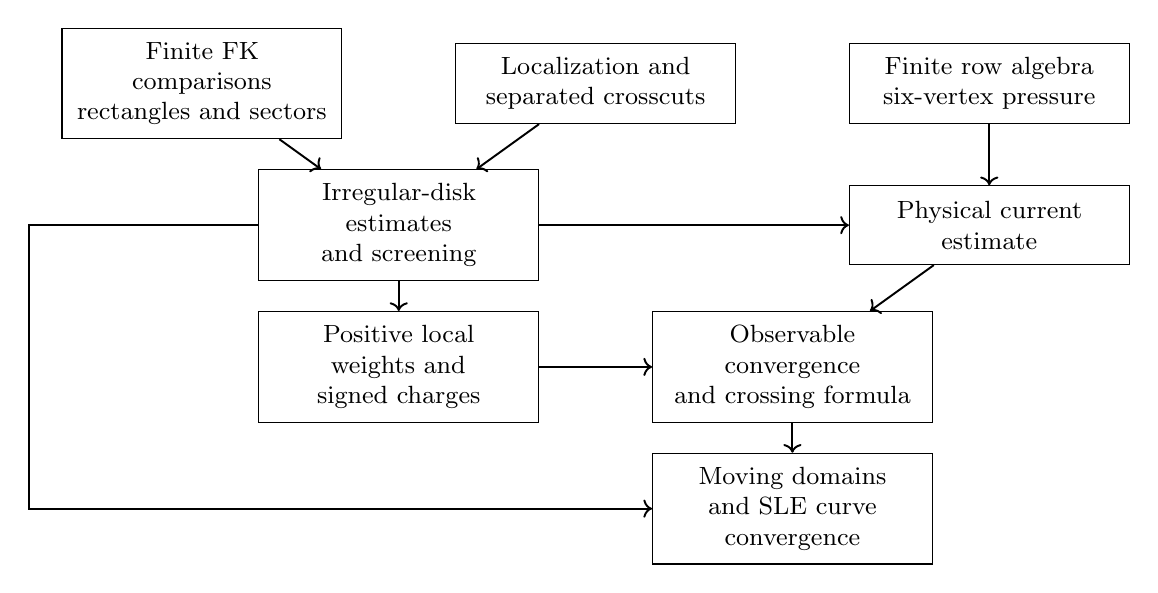
\begin{tikzpicture}[x=1cm,y=1cm,font=\small,
  block/.style={draw,align=center,text width=3.2cm,minimum height=1cm,inner sep=5pt},
  flow/.style={->,line width=.7pt}]
  \node[block] (finite) at (0,0) {Finite FK comparisons\\rectangles and sectors};
  \node[block] (local) at (5,0)
    {Localization and\\separated crosscuts};
  \node[block] (rows) at (10,0) {Finite row algebra\\six-vertex pressure};
  \node[block] (disks) at (2.5,-1.8) {Irregular-disk estimates\\and screening};
  \node[block] (current) at (10,-1.8) {Physical current\\estimate};
  \node[block] (charges) at (2.5,-3.6) {Positive local\\weights and\\signed charges};
  \node[block] (observable) at (7.5,-3.6) {Observable convergence\\and crossing formula};
  \node[block] (sle) at (7.5,-5.4) {Moving domains\\and SLE curve\\convergence};
  \draw[flow] (finite) -- (disks);
  \draw[flow] (local) -- (disks);
  \draw[flow] (rows) -- (current);
  \draw[flow] (disks) -- (current);
  \draw[flow] (disks) -- (charges);
  \draw[flow] (charges) -- (observable);
  \draw[flow] (current) -- (observable);
  \draw[flow] (observable) -- (sle);
  \draw[flow] (disks.west) -- (-2.2,-1.8) -- (-2.2,-5.4) -- (sle.west);
\end{tikzpicture}
\caption{The main proof dependencies. Localization in split tiled disks supplies the clear approaches and separated cuts needed to pass from finite network comparisons to actual-path decay. The disk estimates then feed both the local weight comparisons and the plane interpretation of the current. They also enter the moving-domain argument directly, through crossing estimates uniform over stopped exploration histories.}
\label{fig:dependencies}
\end{figure}


Appendix~\ref{sec:finite-calculus} gives the finite current identities,
extraction formulas, and reflection statements used by the observable.
Its norm consequence additionally uses the physical current estimate.

\section{Finite laws and geometric conventions}\label{sec:conventions}

We fix the finite conditioning, planar duality, and boundary-incidence
conventions used throughout the proof. The distinction between a path
in a quotient graph and a path made of physical open edges is essential:
the comparison inequalities first concern the former, while the
crossing estimates for explored domains must eventually control the latter.

\subsection{Odds, identifications, and conditional laws}

For a finite graph $G=(V,E)$ with positive edge odds $v_e$, write
\begin{equation}\label{eq:odds-partition}
 Z_G(q,\mathbf v)=\sum_{A\subseteq E}q^{k(A)}\prod_{e\in A}v_e.
\end{equation}
Parallel edges and loops are allowed. A boundary partition $\xi$ means
the quotient graph obtained by identifying vertices in each class.
Identifications are not sampled edges. A loop contributes a factor
$1+v_e$ to the partition function and does not affect other edges.
In the square medium all ordinary odds are $v_e=d$.

\begin{lemma}[Finite conditioning and bounded local changes]
\label{lem:finite-conditioning}
Conditioning on any set of edge states gives the random-cluster law on
the remaining graph with the identifications induced by the open
conditioned edges and the original partition. Conditional on all other
edge states, an edge of odds $v$ has opening probability either
$v/(1+v)$ or $v/(q+v)$, according as its endpoints are already connected
or not. Changing a bounded number of edge states or pairwise vertex identifications
therefore has bounded positive weight cost when the affected odds stay
in a fixed compact subset of $(0,\infty)$.
\end{lemma}
\begin{proof}
Contract the open conditioned edges and delete the closed ones.
Components that no longer contain an unconditioned vertex contribute
a fixed power of $q$. All other components are counted in the quotient
graph, giving \eqref{eq:odds-partition}. Adding an edge to a fixed
state either leaves its component count unchanged or reduces it by
one, so its opening-to-closing odds are $v$ or $v/q$.
A single identification of two vertices similarly multiplies a state's weight
by $1$ or $q^{-1}$. Products of a fixed number of such factors, including
the normalizing constants, give the last assertion.
\end{proof}

The same statement applies to a stopped exploration. A leaf of its
decision tree specifies exactly the edge states it has revealed;
no additional event in the uninspected region may be conditioned on
when invoking Lemma~\ref{lem:finite-conditioning}.

\begin{definition}[Network and actual connections]
\label{def:actual-network}
A \emph{network connection} is an open connection in the graph after
the prescribed vertex identifications. An \emph{actual connection}
uses open physical edges and does not jump between distinct vertices
in a boundary class. A measured actual path may subsequently be
contracted to a terminal when its opposite side remains uninspected.
\end{definition}

With only two disjoint separately wired electrode sets, their network
connection is equivalent to an actual path between the sets. Extra
boundary wires can invalidate this equivalence. We will explicitly
remove such shortcuts whenever converting a network test to an actual
path assertion.

\subsection{Tiles, caps, and Euler's identity}

We use checkerboard square tiles whose sides make angle $\pi/4$ with
the primal lattice axes. A tile has one primal diagonal, one dual
diagonal, and a port at each side midpoint. Opening the primal diagonal
pairs the ports around the dual corners; closing it opens the dual
diagonal and pairs the ports around the primal corners. Corners of a
fixed color on one side of a switch strand are connected by actual
edges on that side. The tile drawing only records the same edge state,
not a different random model. Figure~\ref{fig:local-switch} records
the two local states.

\begin{figure}[tbp]
\centering
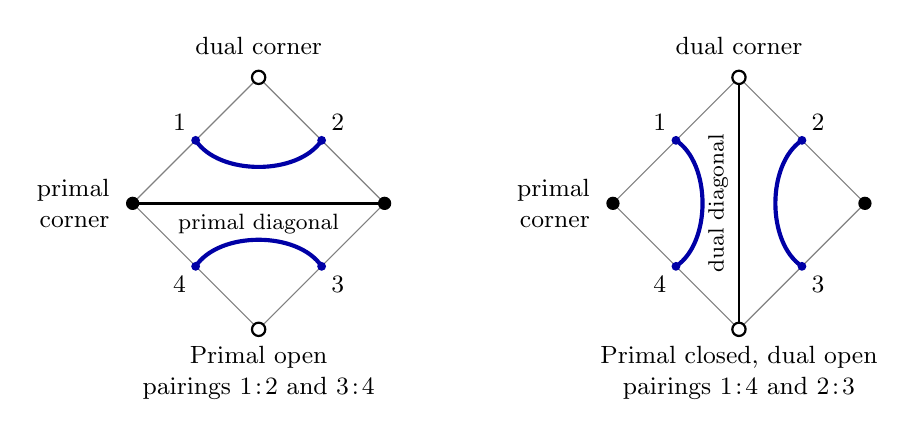
\begin{tikzpicture}[x=1cm,y=1cm,font=\small,line cap=round,line join=round]
  \foreach \shift in {0,6.1} {
    \begin{scope}[xshift=\shift cm]
      \draw[gray] (-1.6,0) -- (0,1.6) -- (1.6,0) -- (0,-1.6) -- cycle;
      \node[above] at (0,1.77) {dual corner};
      \node[left,align=right] at (-1.77,0) {primal\\corner};
      \node[above left] at (-.8,.8) {$1$};
      \node[above right] at (.8,.8) {$2$};
      \node[below right] at (.8,-.8) {$3$};
      \node[below left] at (-.8,-.8) {$4$};
    \end{scope}
  }
  \draw[line width=1pt] (-1.6,0) -- (1.6,0);
  \node[below,font=\footnotesize] at (0,-.015) {primal diagonal};
  \draw[blue!65!black,line width=1.5pt]
    (-.8,.8) .. controls (-.5,.35) and (.5,.35) .. (.8,.8);
  \draw[blue!65!black,line width=1.5pt]
    (-.8,-.8) .. controls (-.5,-.35) and (.5,-.35) .. (.8,-.8);
  \begin{scope}[xshift=6.1cm]
    \draw[line width=1pt] (0,-1.6) -- (0,1.6);
    \node[rotate=90,above,font=\footnotesize] at (-.015,0) {dual diagonal};
    \draw[blue!65!black,line width=1.5pt]
      (-.8,.8) .. controls (-.35,.5) and (-.35,-.5) .. (-.8,-.8);
    \draw[blue!65!black,line width=1.5pt]
      (.8,.8) .. controls (.35,.5) and (.35,-.5) .. (.8,-.8);
  \end{scope}
  \foreach \shift in {0,6.1} {
    \begin{scope}[xshift=\shift cm]
      \fill (-1.6,0) circle (2.4pt);
      \fill (1.6,0) circle (2.4pt);
      \draw[fill=white,line width=.8pt] (0,1.6) circle (2.4pt);
      \draw[fill=white,line width=.8pt] (0,-1.6) circle (2.4pt);
      \foreach \x/\y in {-.8/.8,.8/.8,.8/-.8,-.8/-.8}
        \fill[blue!65!black] (\x,\y) circle (1.6pt);
    \end{scope}
  }
  \node[align=center] at (0,-2.15)
    {Primal open\\pairings $1\!:\!2$ and $3\!:\!4$};
  \node[align=center] at (6.1,-2.15)
    {Primal closed, dual open\\pairings $1\!:\!4$ and $2\!:\!3$};
\end{tikzpicture}
\caption{The two local switch states, with ports numbered clockwise. Black dots are primal corners and white dots are dual corners. The black diagonal is the open physical bond; the complementary diagonal is omitted. Blue curves are medial strands: an open primal bond pairs ports around the dual corners, while an open dual bond pairs ports around the primal corners. The switch drawing records the same FK edge state and introduces no additional randomness.}
\label{fig:local-switch}
\end{figure}


A \emph{wall} cuts tile-to-tile port contractions and keeps its two
banks separate. At a boundary interval designated primal-wired or
dual-wired, local caps pair the intervening ports between successive
visits of the designated vertex color. Boundary-condition changes
leave unmatched ports. A positive
completion pairs the unmatched ports by the specified planar cap
trees, so that the switch diagram is a finite collection of loops.

\begin{lemma}[Positive loop law]\label{lem:loop-law}
For any fixed planar cap completion, the weight of a switch state in
the homogeneous medium is proportional to $d^{\ell}$, where $\ell$
is its number of completed loops and $d=\sqrt q$.
The proportionality factor is independent of the switch state.
Changing a bounded number of loose-port pairings has bounded positive
weight cost for every fixed $d>0$.
\end{lemma}
\begin{proof}
Thicken the open primal graph together with the fixed boundary cap
trees on the sphere. If a planar ribbon graph has $V'$ vertices,
$E'$ edges, and $k'$ components, then its regular neighborhood has
Euler characteristic $V'-E'$ and also $2k'-\ell$, because every
component has genus zero. Thus $\ell=2k'+E'-V'$.
The cap trees change the expression only by a constant depending on
the fixed completion, and their contractions make $k'=k_\xi(A)$.
Consequently
\[
 \ell=2k_\xi(A)+|A|+c_\xi,
 \qquad
 d^\ell=d^{c_\xi}q^{k_\xi(A)}d^{|A|}.
\]
This is the odds form of the FK weight. A change of one pairing can
merge or split only a bounded number of loops. Its weight ratio is
therefore bounded above and below by fixed powers of $d$; normalization
preserves a bounded two-sided comparison.
\end{proof}

On a torus the same thickening has total genus at most one, so the
formula gains $-2g$ with $g\in\{0,1\}$. The loop/FK discrepancy is
then a bounded genus factor. This fact will be used only in the
explicit torus-to-plane comparison of Section~\ref{sec:physical}.

\begin{lemma}[Finite planar duality]\label{lem:finite-duality}
Complementary dual-open edges have odds $q/v_e$. In particular the
homogeneous square medium with odds $d=\sqrt q$ is self-dual.
Complementary boundary caps are understood on the same cut surface.
\end{lemma}
\begin{proof}
For a connected plane graph on the sphere, the dual subgraph on
$E\setminus A$ has as many components as the faces of the primal
subgraph. Euler's identity gives
$k^*(E\setminus A)=|A|-|V|+k(A)+1$.
Multiplying out $q^{k^*(E\setminus A)}
\prod_{e\notin A}(q/v_e)$ shows that its ratio to
$q^{k(A)}\prod_{e\in A}v_e$ is constant in $A$.
Fixed cap trees can be included before applying this identity and
then contracted; their complementary dual incidences give the stated
boundary convention. Disconnected ambient graphs are handled
componentwise or by adding fixed exterior trees.
\end{proof}

\subsection{Cut surfaces and the order of limits}

A tiled disk has an injectively embedded open interior. Boundary
incidences are counted on the disk itself: the two banks of a slit or
the two fans at a pinched vertex are distinct even if their planar
images agree. The specific half-tile and triangular boundary pieces
used below carry the ordinary bonds specified in their construction.
Their conditional law, including any required resampling of cut cells,
is justified when each construction is introduced. A cut does not
identify coincident banks.

A cap partition is \emph{planar} if its classes can be connected by
noncrossing arcs in the designated exterior. A pair of end caps is
\emph{separate} when neither cap joins the two ends. A joint planar
end partition may join them, but is still supported only on those
end intervals. Statements allowing a bounded number of through hubs
will explicitly require that, after removing all classes meeting
those hubs, the residual caps remain separately planar. No assertion
about arbitrary crossing partitions is implicit.

An extremal search starts from a specified exterior complementary face.
It queries an edge only from a reached face and enters the opposite face
only when the intervening edge of the tested color is closed. After
exploring the complete reached component, it selects the appropriate
simple frontier from the measured open edges. On success this frontier
is a blocker whose opposite side remains uninspected. Boundary access
arcs used to define the search do not identify vertices or add physical
edges. Prefixes and stopped leaves retain the cyclic order of the
boundary incidences.

Raw arcs, passages, and nests are counted before the ports at any
wall are paired. This avoids changing a local count by a remote cap
identification. All comparisons concern positive finite laws unless
a signed spin or charge expansion is explicitly specified.

Throughout the paper $q$ is fixed. Constants may depend on $q$,
fixed charges, and fixed shape and buffer parameters. In a geometric
argument the finite inventory of shapes, clearances, gaps, and auxiliary
ratios is chosen before the mesh is sent to zero. A large-circle
transfer limit is taken with the finite insertion diagram fixed;
later mesh or insertion limits follow it. When a relative error is
needed rather than a bounded multiplicative comparison, it is stated
as such. These orders will also be recorded at the points where
several limits interact.

\section{Site pressure and boundary gluing}
\label{sec:pressure}

Throughout this section, $0<q<1$ is fixed, and we put
\[
 u=1-q,\qquad t=q^{-1}.
\]
The graphs are finite and their edge odds are nonnegative and finite,
unless a limiting identification is specified. The basic pressure and
rooted-connection arguments do not require planarity; the cofacial
comparisons additionally use a fixed plane embedding. Together they
provide the restricted connection comparisons used in the geometric
arguments. The proof has three stages. We first obtain nonnegative
coefficients for a site-pressure expansion. Those coefficients give a
rooted multiset representation of connections to an added wire. Finally,
we combine the resulting comparisons with an extremal planar search to
glue connections between interlacing boundary electrodes.
Every result in this section follows from these finite hypotheses.

For a graph $H=(V,E)$, write
\begin{equation}
 Z_H=\sum_{A\subset E}q^{k(V,A)}v_A,
 \qquad v_A=\prod_{e\in A}v_e,
 \label{pressure:partition}
\end{equation}
and let $\PP_H$ be the corresponding FK law. Components include isolated
vertices. A preexisting wire is treated as a vertex identification before
this notation is applied. Thus a vertex of $H$ may represent several
vertices of an earlier physical graph; a path in $H$ need not lift to a
physical path in that earlier graph. We write $\EE_0$ for independent bond
percolation with opening probabilities $v_e/(1+v_e)$ on the same graph.
Loops factor independently out of \eqref{pressure:partition}. Parallel
edges can be replaced by a single edge of odds
$\prod_e(1+v_e)-1$ whenever only connectivity is at issue.

\subsection{A positive expansion of the site pressure}

For a vertex set $C$, put $x_C=\prod_{a\in C}x_a$ and define
\begin{equation}
 F_H(x)=\EE_0\prod_{C\text{ component of }(V,A)}(1-u x_C).
 \label{pressure:polynomial}
\end{equation}
This is a polynomial, affine in each site variable, with $F_H(0)=1$.
The component product is a site-variable form of the external-field
FK expansion in \cite[Section~6]{Sokal2001ComplexZeros}; the hub
calculation below identifies these variables.
At $x=\one_V$, every component contributes $q$, so
\[
 F_H(\one_V)=\frac{Z_H}{\prod_{e\in E(H)}(1+v_e)}.
\]
Site values in $(0,1]^V$ also have a partition-function interpretation.
Adjoin a new vertex $o$ to $H$ and finitely many links from vertices of
$H$ to $o$, allowing several links at a site. For this specialization put
\[
 s_i=\prod_{h:\,i-o}(1+v_h),\qquad x_i=s_i^{-1},
 \qquad s_C=\prod_{i\in C}s_i,
\]
where an empty product is one. For a fixed original open graph, summing
the hub links at a component $C$ gives weight $q$ if none is open and
weight $s_C-1$ otherwise, with one further global factor $q$ for the
hub component. Consequently
\begin{equation}
 Z_{H+o}=q\left(\prod_{e\in E(H)}(1+v_e)\right)
              \left(\prod_{i\in V}s_i\right)F_H(1/s).
 \label{pressure:hub-partition}
\end{equation}
We will use the next theorem to control how this partition function
changes with the hub links. Its coefficient signs will also turn a
derivative at a vertex into a probability law.

\begin{theorem}[Positive site pressure]
\label{thm:pressure}
There are coefficients $c_m\ge0$, indexed by the nonzero multiindices
$m\in\Z_{\ge0}^{V}$, such that
\begin{equation}
 -\log F_H(x)=\sum_{m\ne0}c_m x^m,
 \qquad x^m=\prod_{i\in V}x_i^{m_i}.
 \label{pressure:series}
\end{equation}
The series converges absolutely on a polydisk containing the closed
unit polydisk in its interior. If $c_m>0$, the support
$\{i:m_i>0\}$ is connected in $H$.
\end{theorem}

\begin{proof}
We first identify the squarefree coefficients of $F_H$, then the signs
of its logarithmic coefficients, and finally the convergence domain.
The sign argument uses labeled copies of vertices: an auxiliary
cancellation removes repeated types before the logarithm is taken.

\paragraph{The coefficients of the site polynomial.}
Discard loops and combine parallel edges, so that $H$ is simple. Set
\[
 \gamma_i=\prod_{e\ni i}(1+v_e)^{-1},\qquad y_i=\gamma_i x_i.
\]
Selecting a collection of components in
\eqref{pressure:polynomial} with union $T$ forces every edge between $T$
and its complement to be closed. Summing all edges in the complement
therefore shows that the coefficient of $y_T$ is
\begin{equation}
 W(T)=\prod_{e\in E(H[T])}(1+v_e)
       \sum_{A\subset E(H[T])}v_A(-u)^{k(T,A)}.
 \label{pressure:squarefree}
\end{equation}
Indeed, the factors $\gamma_i$ count each internal edge twice, whereas
the percolation normalization counts it once. This accounts for the
first product in \eqref{pressure:squarefree}. Coefficients with a
repeated variable vanish.

\paragraph{Connected structures and logarithmic signs.}
To take the logarithm, use a finite set $U$ of labeled elements, each
carrying a type in $V$; there are $m_i$ elements of type $i$. Repeated
types are needed because a logarithm need not be squarefree, even when
$F_H$ is. The two ordinary edge sets below represent, respectively,
the partition sum and the extra product in
\eqref{pressure:squarefree}; hard edges cancel repeated types before
the connected-structure restriction is imposed. Between
elements of distinct adjacent types allow an ordinary edge with the
corresponding odds $v_e$. Between elements of the same type allow a
hard edge. For a subset $J\subset U$, independently choose two sets
$A,B$ of ordinary edges and a set $L$ of hard edges, and give the
resulting structure weight
\begin{equation}
 v_Av_B(-u)^{k(J,A)}(-1)^{|L|}.
 \label{pressure:structure-weight}
\end{equation}
If a type repeats in $J$, summation over a possible hard edge cancels
the full sum. If no type repeats, summation over $B$ gives the first
product in \eqref{pressure:squarefree}, and the full sum is $W(T)$.
Consequently the sum of \eqref{pressure:structure-weight} is the mixed
derivative of $F_H$ at zero in the labeled $y$-slots $J$.

The weight factors over the connected components of $A\cup B\cup L$.
In particular the number of $A$-components is additive over those
components. Decomposing every structure according to its partition
into connected components proves the labeled exponential formula in
this setting: the mixed derivative of $\log F_H$ in the slots $U$ is
the same sum restricted to structures with $A\cup B\cup L$ connected.
This is an identity of formal series; no convergence assertion is
being used yet.
For the corresponding connected-graph logarithm in the hard-core gas,
see \cite[Proposition~2.1]{ScottSokal2005RepulsiveGas}.

We group this connected sum by the ordinary-edge union $D=A\cup B$.
If $(U,D)$ has $b$ components, the ordinary-edge sum has sign
$(-1)^b$ or vanishes, while the connected hard-edge sum has sign
$(-1)^{b-1}$ or vanishes. Their product gives the required nonpositive
sign for the logarithmic derivative.

For fixed $D$, an edge of $D\setminus A$ must
belong to $B$ and contributes $v_e$. An edge of $A$ may or may not
belong to $B$, and contributes $v_e(1+v_e)$. Thus summing over $A,B$
with union $D$ gives
\begin{equation}
 v_D\prod_{D_0}Z(D_0;-u,1+v),
 \qquad
 Z(G;s,w)=\sum_{R\subset E(G)}s^{k(V(G),R)}w_R,
 \label{pressure:fixed-union}
\end{equation}
where $D_0$ ranges over the connected components of $(U,D)$.

For every connected graph $G$ and weights $w_e\ge1$, one has
\begin{equation}
 Z(G;-u,w)<0.
 \label{pressure:negative-partition}
\end{equation}
This is a special case of \cite[Theorem~4.4]{JacksonSokal2009TutteZeros},
where the result is attributed to Dong. Here is a direct induction
for the present weights, including multigraphs. A loop contributes a
positive factor $1+w_e$. A bridge can be contracted at the positive
factor $w_e-u$. For an edge that is neither a loop nor a bridge,
deletion and contraction both leave connected graphs, and
\[
 Z(G;-u,w)=Z(G\setminus e;-u,w)+w_e Z(G/e;-u,w)
\]
is the sum of two negative terms. The initial graph with one vertex
and no edges has partition function $-u$. This proves
\eqref{pressure:negative-partition}.

It remains to sum the hard edges, subject to $D\cup L$ being connected.
If a possible hard edge lies within a $D$-component, its two choices
cancel because it has no effect on this connectivity requirement.
Otherwise contract all $D$-components. The hard-edge sum becomes
\[
 \sum_{L:\,([b],L)\text{ connected}}(-1)^{|L|},
 \qquad b=k(U,D),
\]
on a hard multigraph with $b$ vertices. This sum is either zero or has
sign $(-1)^{b-1}$. To see this directly, loops cancel, disconnected
graphs have sum zero, and the deletion-minus-contraction recursion
preserves the asserted sign; the one-vertex graph has value one.
The $b$ factors in \eqref{pressure:fixed-union} have sign $(-1)^b$.
Their product with the hard-edge sum is therefore nonpositive.
Each contribution grouped by the ordinary union $D$, after summing
the hard edges, is therefore nonpositive. Dividing by the positive
factorials of the multiplicities
and rescaling from $y$ to $x$ proves $c_m\ge0$.

A connected structure on the labeled elements projects to a connected
set of vertex types: hard edges only join equal types and ordinary
edges project to edges of $H$. This proves the assertion about support.
The hard-edge sign and connected-support conclusions are the
repulsive-gas principles of
\cite[Propositions~2.8--2.9]{ScottSokal2005RepulsiveGas} after the
ordinary-union regrouping above; the argument here proves them directly
for this site polynomial.

\paragraph{Convergence beyond the unit polydisk.}
The preceding arguments are formal coefficient identities. To use their
derivatives as probabilities, we must also justify convergence at
$x_i=1$. The following direct nonnegative-series argument is the finite form of
the convergence principle in \cite[Theorem~2.10]{ScottSokal2005RepulsiveGas}.
For $x\in[0,1]^V$, every factor in
\eqref{pressure:polynomial} is at least $q$, so $F_H(x)>0$.
The diagonal series
\[
 G(z)=\sum_{m\ne0}c_m z^{|m|}
\]
has nonnegative coefficients and a positive radius of convergence,
because it initially equals $-\log F_H(z,\ldots,z)$ near zero.
Suppose its radius $R$ were finite and at most one. Positivity of
$F_H$ on the real interval gives an analytic continuation of this
germ through a neighborhood of $R$. For each derivative order,
monotone convergence as $z\uparrow R$ identifies the nonnegative
coefficient sum at $R$ with the corresponding finite derivative
$G^{(j)}(R)$. For small $h>0$, Taylor expansion at $R$ and summation
of nonnegative terms would then give
\[
 \sum_{m\ne0}c_m(R+h)^{|m|}
   =\sum_{j\ge0}\frac{G^{(j)}(R)}{j!}h^j<\infty,
\]
contrary to the definition of $R$. Thus $R>1$ (or $R=\infty$).
For any $1<r<R$, the diagonal sum bounds the absolute sum on
$|x_i|\le r$. The negative of the series exponentiates to $F_H$, since this
identity holds near zero and hence throughout the polydisk.
The series agrees with the real negative logarithm on the unit cube.
\end{proof}

We record two consequences of the proof that will be useful when
comparing pressure coefficients in different local graphs.

\begin{lemma}[Locality and identification of zero sites]
\label{pressure:coefficient-locality}
For a simple graph and a fixed multiindex $m$, write
\begin{equation}
 c_m=\left(\prod_i\gamma_i^{m_i}\right)b_m.
 \label{pressure:incident-factors}
\end{equation}
Then $b_m\ge0$ depends only on the induced graph on $\supp(m)$ and
its odds, and is nondecreasing in each of these odds. Thus decreasing
the incident products $\prod_{e\ni i}(1+v_e)$ at support vertices,
with the induced graph unchanged, cannot decrease $c_m$.

If variables on a set $S$ are fixed to zero, identifying any groups
of vertices within $S$ does not change $F_H$ as a polynomial in the
remaining variables, provided the new identified vertices also have
site variable zero. In particular all pressure coefficients whose
support avoids $S$ remain unchanged under these identifications.
\end{lemma}

\begin{proof}
The labeled construction above involves only types in $\supp(m)$.
After the factors in \eqref{pressure:incident-factors} are extracted,
$b_m$ is a finite sum of nonnegative contributions, one for each
ordinary union $D$. Apart from a nonnegative integer from the
hard-edge sum and a positive factorial denominator, each contribution
is
\[
 v_D\prod_{D_0}\bigl[-Z(D_0;-u,1+v)\bigr].
\]
For a connected graph, differentiating $Z$ with respect to a nonloop
weight gives the partition function of its contraction, which is
negative by \eqref{pressure:negative-partition}; differentiating in
a loop weight gives the partition function with that loop removed,
also negative. Hence every factor $-Z$ is nondecreasing in the edge
weights. Adding an allowed induced edge merely adds nonnegative
terms as well. This proves the first assertion, with parallel edges
combined before applying it.

For the second assertion, fix the states of the original edges.
Every component meeting $S$ has factor one in
\eqref{pressure:polynomial}. Identifying vertices in $S$ only merges
some of these components and leaves all other components unchanged.
The product of factors is therefore unchanged for every edge state.
The independent edge law is unchanged as well; edges that become
loops can be retained. Taking expectations proves the polynomial
identity, and taking its logarithm at zero proves the coefficient
identity.
\end{proof}

\subsection{Hub links and restricted correlation inequalities}

Return to the augmented graph and the products $s_i$ in
\eqref{pressure:hub-partition}. The pressure expansion now gives
comparison inequalities for its incident links.

\begin{lemma}[Adjacent and cofacial Rayleigh inequalities]
\label{lem:adjacent-rayleigh}
In every finite FK graph with $0<q<1$, two distinct edges incident to
a common vertex have nonpositive covariance of their opening
indicators. In a plane graph the same conclusion holds for two
distinct edges incident to a common face. Both statements remain
valid after deleting or contracting any other edges.
\end{lemma}

\begin{proof}
Regard the common vertex as $o$, remove it to obtain $H$, and regard
its incident nonloop edges as hub links. By
\eqref{pressure:hub-partition} and Theorem~\ref{thm:pressure}, the part
of $\log Z_{H+o}$ depending on those links is
\begin{equation}
 \sum_h\log(1+v_h)
 -\sum_{m\ne0}c_m\prod_h(1+v_h)^{-m_{i(h)}}.
 \label{pressure:hub-log}
\end{equation}
Every monomial in the second sum has nonnegative mixed derivative
in the odds of two distinct links, including links at the same site.
The first sum has mixed derivative zero. Absolute convergence on a
larger polydisk justifies termwise differentiation, including at
zero link odds by continuity. Thus
$\partial_{v_e}\partial_{v_f}\log Z\le0$ for distinct incident edges.
For positive odds,
\begin{equation}
 \partial_{v_e}\partial_{v_f}\log Z
  =\frac{\Cov(\one_{\{e\text{ open}\}},
                     \one_{\{f\text{ open}\}})}{v_ev_f}.
 \label{pressure:rayleigh-derivative}
\end{equation}
Loops are independent of all other edge states and cause no exception.

For the plane statement, complementary dual edges have odds $q/v_e$.
Two primal edges on a common face become two dual edges at a common
vertex. Complementing both opening indicators preserves their
covariance, so the adjacent inequality in the dual gives the claimed
cofacial inequality. Zero odds and contraction limits follow by
continuity of finite partition functions after removal of their
common leading factors.
\end{proof}

\begin{lemma}[Monotonicity of tested network connections]
\label{pressure:network-monotonicity}
Let $a,o$ be vertices in a finite graph. Adding or strengthening an
edge incident to $o$ does not decrease $\PP(a\leftrightarrow o)$. The same
holds in a plane graph if the added edge and an auxiliary connection
test edge from $a$ to $o$ can be drawn cofacially in the graph
containing both edges. In particular, adding vertices to a terminal
by identification does not decrease its connection probability to another
fixed terminal.

For any three vertices $a,b,o$,
\begin{equation}
 \PP(a\leftrightarrow o,\ b\leftrightarrow o)
 \ge \PP(a\leftrightarrow o)\PP(b\leftrightarrow o).
 \label{pressure:root-correlation}
\end{equation}
\end{lemma}

\begin{proof}
Add a distinct auxiliary edge $f$ between $a$ and $o$, initially of
odds zero. Its logarithmic partition derivative is
\begin{equation}
 \left.\partial_{v_f}\log Z\right|_{v_f=0}
 =\PP(a\leftrightarrow o)+q^{-1}\PP(a\not\leftrightarrow o)
 =q^{-1}-(q^{-1}-1)\PP(a\leftrightarrow o).
 \label{pressure:test-edge}
\end{equation}
The mixed derivative with respect to the strengthened edge is
nonpositive by Lemma~\ref{lem:adjacent-rayleigh}. Because
$q^{-1}-1>0$, the tested connection probability is nondecreasing.
The cofacial argument is identical. Sending incident auxiliary odds
to infinity proves the terminal-identification assertion.

For \eqref{pressure:root-correlation}, induct on the number of edges,
discarding loops. If no nonloop edge touches $o$, both tested events
are constant. Otherwise condition on an edge $e$ incident to $o$.
The conditional laws are FK on the deletion and contraction minors,
and their conditional covariance is nonnegative by induction.
Moreover, each of the two conditional means is at least as large
when $e$ is open as when it is closed: vary its odds from zero to
infinity in the connection monotonicity just proved. The covariance
of these two conditional means is consequently nonnegative. The
conditional covariance identity proves the induction step. Cases
in which a tested vertex is contracted to $o$ simply make its event
constant one.
\end{proof}

The pressure coefficients encode more than derivative signs. After
weighting by the multiplicity at a root, they form a probability law
on connected vertex multisets. Wiring a set then becomes the event
that the multiset meets it. In particular, unions of target sets can
be compared in one fixed probability space, even though their FK laws
have different wires. The unrooted coefficients $c_m$ have a second
role: their mass over multisets meeting a set gives its full-wiring
log gain, up to the single constant for the surviving wired component.
The lemma records both forms.

\begin{lemma}[Rooted coverage representation]
\label{lem:rooted}
For $a\in V$, the numbers
\begin{equation}
 \mu_H^a(m)=\frac q u m_a c_m
 \label{pressure:rooted-law}
\end{equation}
define a probability law on finite nonempty vertex multisets with
connected support containing $a$. In the graph with hub links above,
\begin{equation}
 \PP_{H+o}(a\not\leftrightarrow o)
   =\sum_m\mu_H^a(m)x^m.
 \label{pressure:rooted-nonconnection}
\end{equation}
If $S\subseteq V$ is nonempty, let $H/S$ identify precisely the
vertices of $S$, with no other new identifications. Then
\begin{equation}
 \PP_{H/S}(a\leftrightarrow S)
  =\mu_H^a\{m:\supp(m)\cap S\ne\varnothing\}.
 \label{pressure:rooted-hit}
\end{equation}
Here $S$ on the left denotes the collapsed vertex. Equivalently,
adjoin a fresh hub with exactly one infinite-odds link from each site
of $S$ and no other incident links.
Any identifications already represented in $H$ are retained.
Writing $k_S(A)$ for the number of open components meeting $S$,
\begin{equation}
 K_H(S):=\log\EE_H t^{k_S}
  =\sum_{\supp(m)\cap S\ne\varnothing}c_m.
 \label{pressure:coverage}
\end{equation}
In particular $K_H$ is a nonnegative coverage function,
$K_H(\{a\})=\log t$, and
\begin{equation}
 K_H(S)+K_H(T)-K_H(S\cup T)
 =\sum_{\substack{\supp(m)\cap S\ne\varnothing\\
                   \supp(m)\cap T\ne\varnothing}}c_m\ge0.
 \label{pressure:double-coverage}
\end{equation}
\end{lemma}

\begin{proof}
Differentiate \eqref{pressure:hub-partition} with respect to $s_a$:
\begin{equation}
 s_a\partial_{s_a}\log Z_{H+o}
       =1+\sum_m m_a c_m x^m.
 \label{pressure:hub-derivative}
\end{equation}
This derivative has a second interpretation. Conditional on the
original open graph, the component $C_a$ has hub-link factor
$s_{C_a}-u$. Its contribution to the derivative is
\[
 \frac{s_{C_a}}{s_{C_a}-u}
   =1+\frac{u}{s_{C_a}-u},
\]
while its conditional probability of having no hub link is
$q/(s_{C_a}-u)$. Averaging under the marginal original-edge law of
the augmented graph and comparing with
\eqref{pressure:hub-derivative} proves
\eqref{pressure:rooted-nonconnection}. At $s_i=1$ for every $i$, the
hub is isolated, so the right side equals one. Nonnegativity and the
support assertion now follow from Theorem~\ref{thm:pressure}.
For the $H/S$ specialization, adjoin a fresh hub with links only at
$S$ and send their odds to infinity. Then $x_i=0$ on $S$ and $x_i=1$
elsewhere, giving \eqref{pressure:rooted-hit}, including when $a\in S$.

For \eqref{pressure:coverage}, put $x_i=\one_{\{i\notin S\}}$ in
\eqref{pressure:polynomial}. A component meeting $S$ then contributes
one instead of q. Hence
\[
 \frac{F_H(\one_{V\setminus S})}{F_H(\one_V)}
       =\EE_H q^{-k_S}.
\]
Take logarithms and use \eqref{pressure:series}. For a singleton,
$k_{\{a\}}=1$ in every configuration, so $K_H(\{a\})=\log t$.
The final identity is the inclusion-exclusion identity for the two
support-hitting events in the nonnegative sum.
\end{proof}

The rooted law controls connection probabilities, while
\eqref{pressure:coverage} measures the gain from full boundary wiring.
We first record two quantitative forms of the connection statement.
Adjoin a fresh vertex $o$ with exactly one odds-$v$ link to each site
of $I\subseteq V$ and no other incident links. Then
\begin{equation}
 \PP(a\leftrightarrow o)
 =\EE_{\mu_H^a}\bigl[1-(1+v)^{-N_I}\bigr],
 \qquad N_I=\sum_{i\in I}m_i.
 \label{pressure:finite-spokes}
\end{equation}
In particular this probability is between
$\frac{v}{1+v}\mu_H^a(N_I>0)$ and $\mu_H^a(N_I>0)$, uniformly in
the number of links. Second, if $A$ and $T$ are nonempty disjoint
vertex sets, define
\begin{equation}
 g_H(A,T)=\PP_{H/(A,T)}(A\leftrightarrow T),
 \label{pressure:network-g}
\end{equation}
where each of the two sets is separately identified. In this law,
connection is equivalent to an open path in the represented base
graph $H$ from a vertex of $A$ to a vertex of $T$, using no hop from
either of these two new wires. Indeed a shortest quotient connection has
a segment from its last departure from the first wire to its first
arrival at the second wire with no wire hop in between.
If the edges of $H$ are physical edges and each vertex is a single
physical vertex, this is an actual physical path. If $H$ arose from
an earlier physical graph by other identifications, the path may pass
through one of those quotient vertices. Recovering a path in the earlier
physical graph then requires an explicitly available open connection
between the incidences used at each such class.
Apply \eqref{pressure:rooted-hit} on the fixed graph $H/A$ with root
the collapsed $A$. The union bound under this single multiset law
gives
\begin{equation}
 g_H(A,T_1\cup T_2)\le g_H(A,T_1)+g_H(A,T_2),
 \label{pressure:subadditivity}
\end{equation}
whenever both target sets are disjoint from $A$. They need not be
disjoint from each other. Symmetry gives the corresponding assertion
for the first terminal.

\subsection{A no-hit comparison without planarity}

It is important not to confuse the preceding network monotonicity
with the effect of wiring the target of an as-yet unwired hit event.
For that operation the comparison has the opposite direction.

\begin{lemma}[Wiring an unwired target]
\label{pressure:general-no-hit}
Let $a$ be a vertex and $S$ a nonempty vertex set in any finite graph
$H$. The probability that the open component of $a$ meets $S$ is at
least its probability after all vertices of $S$ have been identified:
\begin{equation}
 \PP_H(a\leftrightarrow S)
   \ge \PP_{H/S}(a\leftrightarrow S).
 \label{pressure:general-hit-comparison}
\end{equation}
The original graph may already contain identifications, including a
wire represented by the root $a$.
\end{lemma}

\begin{proof}
If $a\in S$, both probabilities are one. Otherwise induct on the
number of edges, ignoring independent loops. If no nonloop edge is
incident to $S$, both probabilities are zero. Choose a nonloop edge
$e$ with endpoint $s\in S$. Write $\mu=\PP_H$, $\nu=\PP_{H/S}$, and
let $\alpha,\beta$ be their respective probabilities that $e$ is open.
To form $H/S$, add auxiliary links from $s$ to all other vertices of
$S$ and send their odds to infinity. Every such link is incident to
$e$. Lemma~\ref{lem:adjacent-rayleigh} therefore gives
\begin{equation}
 \alpha\ge\beta.
 \label{pressure:target-edge-marginal}
\end{equation}

For $j=0,1$, let $h_j$ and $\widetilde h_j$ be the conditional hit
probabilities under $\mu$ and $\nu$, respectively, given the state
$j$ of $e$. Conditional FK laws are deletion and contraction minors.
Identification of $S$ commutes with both operations, with its image
used after contraction. The induction hypothesis therefore gives
$h_j\ge\widetilde h_j$. If $e$ becomes a loop in $H/S$, its state is
independent of the hit event and $\widetilde h_1=\widetilde h_0$.
Otherwise it is incident to the collapsed target terminal, and
Lemma~\ref{pressure:network-monotonicity} gives
$\widetilde h_1\ge\widetilde h_0$. Thus
\begin{align*}
 \PP_H(a\leftrightarrow S)
 &=\alpha h_1+(1-\alpha)h_0\\
 &\ge\alpha\widetilde h_1+(1-\alpha)\widetilde h_0\\
 &\ge\beta\widetilde h_1+(1-\beta)\widetilde h_0
  =\PP_{H/S}(a\leftrightarrow S).
\end{align*}
If contraction brings $a$ into the image of $S$, the corresponding
conditional probabilities are both one. Zero odds are obtained by
continuity, or by deleting those edges at the start.
\end{proof}

\subsection{Cofacial partition gains}

We next isolate the partition-function form of cofacial comparison.
It will also justify erasing an exposed component in later cap
arguments. A plane graph here has a fixed tame embedding; incidences
on different banks of a cut are distinct incidences.

\begin{lemma}[Cofacial gain and exposed erasure]
\label{pressure:cofacial-gain}
Let $X$ be a finite collection of auxiliary edges between vertices
of a plane graph $K$, and let $h$ be an original edge. Suppose that, in the
drawing containing all these edges, $h$ and each edge of $X$ are
cofacial. For fixed nonnegative auxiliary odds, the gain
\begin{equation}
 \frac{Z_{K+X}}{Z_K}
 \label{pressure:gain}
\end{equation}
is nonincreasing in the odds of $h$.

In particular, suppose $B\ne\varnothing$, $X$ is an auxiliary tree
with vertex set exactly $B$, and the drawing of $K+X$ has a face incident to a
vertex $a$ and to every edge of $X$. Let $U$ be a connected vertex
set in $K$ containing $a$ and disjoint from $B$. Then
\begin{equation}
 \EE_{K-U}t^{k_B-1}\ge\EE_K t^{k_B-1}.
 \label{pressure:erasure-gain}
\end{equation}
The same conclusion holds if $U$ is the vertex set of an open
component containing $a$.
\end{lemma}

\begin{proof}
Raise the auxiliary odds successively from zero to their prescribed
values. The logarithm of \eqref{pressure:gain} is the sum of the
integrals of $\partial_{v_f}\log Z$ for $f\in X$ during these changes.
Its derivative with respect to the odds of $h$ is nonpositive by the
cofacial assertion of Lemma~\ref{lem:adjacent-rayleigh}. This proves
the first statement; all embeddings are kept fixed, even when an
edge has odds zero.

For the second, delete the edges of $K$ incident to $U$ in an exposed
order. Start at the face sector incident to $a$. Once one sector at
a vertex of $U$ is exposed, delete its incident edges successively
around its cyclic fan, thereby enlarging the same face. An edge
leading to another vertex of $U$ exposes a sector there. A spanning
tree of the connected set $U$ ensures that this procedure reaches
every vertex of $U$. All original edges incident to $U$ can therefore
be deleted, and every edge at its deletion borders the expanding
face. The edges of $X$ remain on its boundary, because none touches
$U$ and deleting an edge never splits a face. If the deleted edge
has the same face on both sides, that face remains available along
both banks; otherwise its two incident faces merge. A loop can be removed
without affecting any gain. At each step the first part of the
lemma shows that the auxiliary-edge gain cannot decrease. Isolated
vertices left in $U$ contribute the same factors to numerator and
denominator and can be discarded.

Finally send every auxiliary odds to infinity and divide the gain
by their product. For a fixed original edge state, the tree $X$
identifies all $k_B$ components meeting $B$, changing the cluster
count by $-(k_B-1)$. The limiting gain is consequently
$\EE_K q^{1-k_B}$, and after erasure it is
$\EE_{K-U}q^{1-k_B}$. This proves
\eqref{pressure:erasure-gain}. An open component is connected in the
underlying graph, so it satisfies the same geometric hypothesis.
\end{proof}

For example, if $a$ does not hit $B$ and one conditions on its
component vertex set $U$, the unremoved graph has FK law on $K-U$.
The weight for additionally wiring $B$ is $t^{k_B-1}$.
Equation~\eqref{pressure:erasure-gain} says that its conditional mean
on this no-hit event is at least its unconditional mean. Weighting
by it therefore does not decrease the no-hit probability. This gives a
planar partition-gain proof of the special case of
Lemma~\ref{pressure:general-no-hit} used below, as well as the more
explicit erasure comparison needed for boundary partitions.

\subsection{Interlacing boundary connections}

Let $H$ be embedded in a topological closed disk. An electrode is a
nonempty set of boundary vertices contained in a specified closed
boundary arc. We require that its vertices are accessible from the
exterior on that arc: an arbitrarily small outward extension can
reach them without crossing the graph. Separate electrodes below
lie on disjoint such arcs; unmarked vertices may occupy the gaps.
This convention includes ordinary lattice polygons and their cut
surfaces.

Figure~\ref{fig:interlacing} shows the separation geometry in an
ordinary physical graph. The probability inequality requires the conditional argument below,
since its two input probabilities have different boundary wires.
\begin{figure}[tbp]
\centering
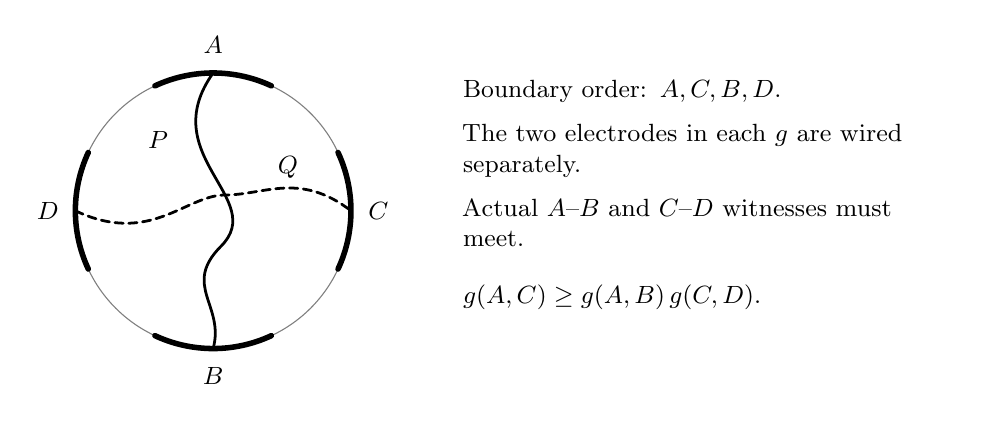
\begin{tikzpicture}[x=1cm,y=1cm,font=\small,line cap=round,line join=round]
  \draw[gray] (0,0) circle (1.75);
  \foreach \start/\finish/\name/\angle in {65/115/A/90,-25/25/C/0,-115/-65/B/-90,155/205/D/180} {
    \draw[line width=2pt] (\start:1.75) arc (\start:\finish:1.75);
    \node at (\angle:2.1) {$\name$};
  }
  \draw[line width=1pt] (0,1.75) .. controls (-.75,.7) and (.7,.15) .. (.1,-.45)
    .. controls (-.4,-.95) and (.15,-1.2) .. (0,-1.75);
  \draw[densely dashed,line width=1pt] (-1.75,0) .. controls (-.8,-.45) and (-.35,.2) .. (.15,.2)
    .. controls (.65,.2) and (1.1,.5) .. (1.75,0);
  \node[fill=white,inner sep=1.5pt] at (-.7,.9) {$P$};
  \node[fill=white,inner sep=1.5pt] at (.95,.55) {$Q$};
  \node[align=left,anchor=west,text width=6.1cm] at (3.05,.6)
    {Boundary order: $A,C,B,D$.\\[5pt]
     The two electrodes in each $g$ are wired separately.\\[5pt]
     Actual $A$--$B$ and $C$--$D$ witnesses must meet.};
  \node[anchor=west] at (3.05,-1.1)
    {$g(A,C)\geq g(A,B)\,g(C,D)$.};
\end{tikzpicture}
\caption{The topology behind interlacing gluing. Thick boundary arcs mark the four electrode sets, not a common four-wire law: each probability $g$ wires only its own two electrodes. The curves $P,Q$ illustrate actual witnesses and their forced meeting, not simultaneous events under one boundary condition. The probability inequality uses the restricted comparison and the extremal exploration in Lemma~\ref{lem:interlacing}, not positive association or independence.}
\label{fig:interlacing}
\end{figure}


\begin{lemma}[Interlacing gluing]
\label{lem:interlacing}
Suppose four electrodes occur in cyclic order $A,C,B,D$ on the
boundary of one disk. With $g_H$ defined by
\eqref{pressure:network-g},
\begin{equation}
 g_H(A,C)\ge g_H(A,B)\,g_H(C,D).
 \label{pressure:interlacing}
\end{equation}
The edge odds may be arbitrary nonnegative finite numbers. The disk
embedding and electrode-access assumptions are imposed after any
preexisting identifications. Apart from the two wires specified in
each $g_H$, there are no further abstract ties between distinct
vertices of this embedded graph.
All path witnesses in the proof use edges of this represented graph
$H$ before the electrode wires are added. If $H$ is a quotient of an
earlier physical graph, the statement alone does not assert that those
paths lift to physical paths in the earlier graph.
\end{lemma}

\begin{proof}
Our base law has $A,C$ separately wired. First we compare an
$A$--$B$ path in $H$ with a network hit. We then expose
an extremal such witness and compare the uninspected $C$ side with
the separate $C,D$ network. The two comparisons will give the two
factors on the right of \eqref{pressure:interlacing}.

\paragraph{From a network hit to a path in $H$.}
Denote the collapsed $A$ by $a$. Lemma~\ref{pressure:general-no-hit} says that the
probability that the component of $a$ hits the as-yet unwired set
$B$ is at least the corresponding probability when $B$ is also
wired. In the latter law, its $A$-to-$B$ connection probability is
at least $g_H(A,B)$. Indeed, realize the additional $C$ wire by a
chain of exterior links along its arc. This chain and a test edge
joining exposed representatives of $A$ and $B$, drawn farther
outside, are cofacial. Apply
Lemma~\ref{pressure:network-monotonicity} and then take the wire
limits.

Let $S$ be the event that there is an open path in $H$ from
$A$ to $B$, using no electrode identification as a hop. If $a$ hits $B$
in the $A,C$ quotient but $S$ fails, a shortcut through $C$ must have
been used. The initial part of such a quotient path, through its
first visit to $C$ and after its last departure from $A$, is an
open $A$-to-$C$ path in $H$. Jumps within $A$ alone cannot produce
a hit of $B$ without an open $A$-to-$B$ path in $H$. Consequently, writing
$T=\{A\leftrightarrow C\}$ in the current law,
\begin{equation}
 \PP(S)+\PP(T\cap S^c)\ge g_H(A,B).
 \label{pressure:physical-hit}
\end{equation}

\paragraph{A measured separator with an uninspected side.}
We now expose such an $A$-to-$B$ path from the $D$ side, leaving
its $C$ side uninspected. Here are explicit details, including
boundary contacts. Only for the search, add disjoint exterior spokes
from $A$ to a terminal $s$ and from $B$ to a terminal $s'$. The
spokes are declared traversable by the search; they are not sampled
edges and do not add any FK identifications. Choose a slightly
enlarged disk with $s,s'$ on its boundary so that the spoke interiors
are inside it. The electrode accessibility assumption lets each
$C$ vertex retain access to the boundary arc on one side of $s,s'$
and each $D$ vertex retain access to the other, without crossing a
spoke or a graph edge. Call these the $C$ and $D$ sides.

Split the exterior face at $s,s'$ and seed the search only at its
$D$-side face. Query an edge from a reached face and enter its opposite
face only when that primal edge is closed. Process the edges incident
to reached faces until the $C$ side is reached or no such unqueried
edge remains. Empty regions of the drawing can be subdivided by dummy
closed edges, whose dual crossings are free; this merely formalizes
the face search. The finite planar path/cut alternative
says that it reaches the other side exactly when there is no open
$s$-to-$s'$ path. One proof is to trace the boundary of the primal
vertices reachable from $s$: in the absence of the connection,
this boundary contains a separating closed-primal dual crosscut.
Conversely, such a crosscut intersects every primal connection.
An open $s$-to-$s'$ path is equivalent to $S$.

On $S$, the explored dual component is exhausted on the $D$ side.
Every edge on its frontier was queried and is open if it prevents
further dual exploration. Setting every unqueried edge of $H$
closed cannot enlarge the explored dual component, since all
edges incident to it have already been queried. The path/cut
alternative therefore still supplies an open $s$-to-$s'$ path in
this modified configuration. Choose a simple such path by a fixed
deterministic rule. It consists of queried open edges and exactly
one initial and one final spoke, so its portion $\gamma$ in $H$
is an open $A$-to-$B$ path determined by the exploration
record.

No reached face is strictly on the $C$ side of this simple path:
the explored dual component starts on the other side and cannot
cross an open primal path or an exterior spoke. Hence no edge of $H$
whose interior is strictly on the $C$ side was queried. If
$\gamma$ meets $C$, event $T$ already holds. Otherwise all $C$
vertices lie on its $C$ side, while all $D$ vertices lie on its
$D$ side or on the path. These assertions follow also for original
boundary contacts by using the retained exterior access curves in
the enlarged disk.

\paragraph{The conditional connection comparison.}
Condition on a successful search record for which $\gamma$ does
not meet $C$. Finite FK domain Markov gives the ordinary FK law on
the unqueried graph with identifications induced by the queried
open connections and the original $A,C$ wires. Restricting to the
right, or $C$-side, subgraph, this means that $\gamma$ is wired,
any $A$ vertices on that side are tied to it, and $C$ is wired
separately. The rest attaches only through the path or that same
$A$ wire. There are no additional ties from the fictitious $B$
spokes: they were only a device for defining the search. Integrating
the other side therefore introduces no further boundary condition.

Dropping the extra $A$ vertices from the first terminal cannot increase
its tested connection probability by
Lemma~\ref{pressure:network-monotonicity}. The conditional chance
of $T$ is consequently at least the pure $\gamma$-to-$C$ network
probability in this right subgraph. To compare that probability
with $g_H(C,D)$, start instead in the full $C,D$-wired graph and add
all vertices of $\gamma$ to the $D$ terminal. This cannot decrease its
connection probability to $C$. After this identification, the
entire left subgraph, including $D$, attaches to the right subgraph
through one wired vertex. FK partition functions factor across a
one-vertex attachment: if $H_1,H_2$ meet at just a wired vertex,
then $k(A_1\cup A_2)=k(A_1)+k(A_2)-1$, so the extra partition
factor cancels from all probabilities determined on $H_1$.
Thus the enlarged-terminal probability in the full graph is exactly
the pure $\gamma$-to-$C$ probability on the right. It follows that
\begin{equation}
 \PP(T\mid\text{successful search record})\ge g_H(C,D).
 \label{pressure:conditional-interlacing}
\end{equation}
The same inequality is automatic if $\gamma$ already meets $C$.

This decomposition remains valid if the simple path touches the
original boundary several times: work in the enlarged disk,
assign off-path edge interiors to their respective sides, and
observe that the only shared graph vertices are path vertices.
Any loops created at the wire are independent and cancel.
The search is adaptive but queries only determined edge states;
conditioning on a record is exactly a finite domain Markov
conditioning and imposes no event on the unqueried right edges.

Average \eqref{pressure:conditional-interlacing} over the successful
records. Since $g_H(C,D)\le1$, \eqref{pressure:physical-hit} yields
\begin{align*}
 g_H(A,C)=\PP(T)
 &\ge g_H(C,D)\PP(S)+\PP(T\cap S^c)\\
 &\ge g_H(C,D)\bigl[\PP(S)+\PP(T\cap S^c)\bigr]\\
 &\ge g_H(C,D)g_H(A,B),
\end{align*}
as required.
\end{proof}

\begin{remark}[Scope of the comparisons]
\label{pressure:scope}
The inequalities above concern tested network connections, rooted
connection events, or specified cofacial changes. They assert
neither positive association for arbitrary increasing events nor
stochastic monotonicity under arbitrary boundary wiring.
Lemma~\ref{lem:interlacing} is a statement about four interlacing
electrodes in a single disk, not an overlapping-rectangle gluing
principle or an arbitrary-boundary-condition crossing estimate.
\end{remark}

\section{Rectangle networks and boundary partition comparisons}
\label{sec:rectangles}

This section has two outputs. Proposition~\ref{prop:rectangle-rsw}
gives rectangle crossing bounds when the two crossing electrodes are
wired separately and the remaining boundary is ordinary.
Lemmas~\ref{lem:one-sided-density} and~\ref{lem:separate-caps} compare
partition-function gains from caps on separate accessible boundary arcs.
The first output supplies local connections; the second controls how
those connections and local laws change when a region is attached to
its exterior. Both use only the finite comparisons of
Section~\ref{sec:pressure} and planar geometry.

The rectangle argument is by contradiction. Near-square bounds and
interlacing will turn a vanishing crossing probability into many
almost-certain crossings of winding corridors. A geometric packing
bound rules out that conclusion. We prove the packing bound, use it
to establish Proposition~\ref{prop:rectangle-rsw}, and then turn to
the boundary partition comparisons.

Throughout, $0<q<1$ is fixed, $v=\sqrt q$, and $t=q^{-1}$.  For a finite
graph $G$ and two disjoint nonempty vertex sets $A,B$, write
\[
 g_G(A,B)=\PP_{G/(A,B)}(A\leftrightarrow B),
\]
where $G/(A,B)$ means separate contraction of $A$ and $B$.
Unless explicitly specified, the graphs used below consist of physical
edges and have no other identifications. The tested event is connection
of the two quotient vertices. In that setting, this two-wire law is
equivalent to the existence of an actual open path from $A$ to $B$ in
$G$. With additional wires, that equivalence must be checked afresh.

An accessible boundary interval will mean an interval on the boundary of
a topological disk containing its marked vertices in their boundary order,
with all physical-edge incidences on the disk side.  Equivalently, narrow
outward prolongations put each marked vertex in a single boundary slot
with an inward physical-edge fan.  Wires on such an interval can be drawn
as links in a narrow exterior cap.  A noncrossing partition of an interval
means a partition realizable by nonintersecting links in that cap.

\subsection{The permitted finite comparisons}

We first record precisely which consequences of Section~\ref{sec:pressure}
will be used.  Adding vertices to a tested terminal does not decrease $g$:
realize the added contractions by edges incident to that terminal and
apply Lemma~\ref{lem:adjacent-rayleigh} against a connection test edge.
Moreover, Lemma~\ref{lem:rooted} gives
\begin{equation}
 g_G(A,B_1\cup B_2)\le g_G(A,B_1)+g_G(A,B_2)
 \label{rect:subadditivity}
\end{equation}
whenever the electrodes are disjoint from $A$.  Indeed the three
quantities are hitting probabilities under the same rooted-multiset law
on $G/A$.  The analogous inequality holds in the first terminal.

There is also a restricted geometric extension comparison.  To test
connection of two exposed terminals, draw an auxiliary edge between them
in the exterior face and take its odds to zero.  Its partition-function
derivative is
\[
 \PP(\text{connection})+q^{-1}\PP(\text{separation}).
\]
Thus the cofacial form of Lemma~\ref{lem:adjacent-rayleigh} says that
adding or strengthening an edge cofacial with this test edge does not decrease
the tested connection probability.  Auxiliary wire links can first have
finite positive odds and then be contracted by sending those odds to
infinity.

\begin{lemma}[Exposed rectangle extension]
\label{rect:extension}
Suppose that a closed lattice rectangle is contained in a larger closed
lattice rectangle, and that its two terminal intervals lie on the common
boundary and remain accessible from the exterior.  Adding the remaining
rectangle edges, without changing the terminals, does not decrease $g$.
The same conclusion holds for the uses below in which a terminal support
is an interval made of two sides meeting at a corner, provided that the
complement of the smaller closed rectangle has exterior access away from
the terminal intervals.
\end{lemma}

\begin{proof}
Draw successive links along the terminal intervals narrowly outside the
rectangles, and a test edge between exposed representatives in the
remaining main exterior face.  This edge has two incident exterior
sectors.  An edge of the larger rectangle not belonging to the smaller
one has a point outside the smaller closed rectangle.  That point can be
joined through the complement of the smaller rectangle to an exterior
gap away from the wire intervals, crossing only edges to be removed.
Perturb the route off vertices.  Starting from the two test-edge faces,
delete edges encountered on these routes by face expansion.  At each
deletion the edge being removed is cofacial with the test edge.  The
cofacial comparison therefore makes connection no larger after deletion.
The cap links do not obstruct these routes: they lie along the common
boundary intervals, and no added rectangle edge lies in their narrow
outer caps.  Take the wire limits after the finite-odds comparison.
\end{proof}

Lemma~\ref{lem:interlacing} applies to cyclically ordered boundary
electrodes $A,C,B,D$ and gives
\begin{equation}
 g_G(A,C)\ge g_G(A,B)g_G(C,D).
 \label{rect:interlacing}
\end{equation}
The following version covers the endpoint contacts between side intervals
that occur in the square constructions.

\begin{corollary}[Interlacing with endpoint abutments]
\label{rect:interlacing-abutments}
Let $G$ be a finite ordinary graph embedded in a closed disk, with the
edge odds of this section. Let the nonempty electrodes $A,C,B,D$ be
carried, in that cyclic order, by four accessible nondegenerate closed
boundary arcs.
Their relative interiors are pairwise disjoint, and only consecutive
arcs in this cyclic order may share an endpoint. Assume
\[
 A\cap C=A\cap B=C\cap D=\varnothing.
\]
At every shared boundary incidence, the full physical-edge fan lies
on the disk side. In a slightly enlarged disk, choose distinct boundary
points $s,s'$, exterior spokes from $A$ to $s$ and from $B$ to $s'$,
and outward access arcs from every $C$ vertex to one of the two open
components of the enlarged boundary minus $\{s,s'\}$ and from every
$D$ vertex to the other. The spokes and access arcs can be chosen with
interiors disjoint from the graph and from one another. They may meet
only at a designated shared electrode endpoint, except that the $A$
spokes may meet at $s$ and the $B$ spokes at $s'$. Then
\eqref{rect:interlacing} holds.
\end{corollary}

\begin{proof}
The $A,C$ caps are disjoint. In their wired law,
Lemma~\ref{pressure:general-no-hit} still compares a hit of the
as-yet unwired set $B$ with the law that also wires its image, even if
$B$ has a shared endpoint with $C$. In comparing the latter law with
the $A,B$ law, adding the $C$ wire enlarges the $B$ terminal when
$B\cap C\ne\varnothing$; otherwise it is the same exterior cofacial
addition as in Lemma~\ref{lem:interlacing}.
If a hit in the $A,C$ quotient uses $C$ as a shortcut, its first visit
to $C$ already gives the desired connection; otherwise it contains an
open $A$-to-$B$ path in $G$. Thus the initial event comparison in that
proof also remains valid.

Use the spokes and access arcs from the hypotheses in the extremal
search. If its path $\gamma$ meets $C$, the desired connection already
holds. Otherwise the access arcs place every $C$ incidence on the
uninspected side, and every $D$ incidence on the other side or on
$\gamma$. A shared endpoint in $B\cap D$ or $D\cap A$ is permitted
on $\gamma$; if it is not there, its assigned access sector places it
on the $D$ side. Thus the separator-wiring comparison and the
conditional one-vertex factorization in the interlacing proof apply
unchanged. This proves \eqref{rect:interlacing}.
\end{proof}

At each later use in this section, the output electrodes and the two
ends of each input chord are disjoint. Any remaining contact is a
shared corner of consecutive rectangle sides, whose inward physical
fans and separate outward sectors satisfy the corollary.

\subsection{Square and corner bounds}

For integers $w\ge1$ and $h\ge0$, let $R_{w,h}$ be the graph with vertex set
$\{0,\ldots,w\}\times\{0,\ldots,h\}$ and all nearest-neighbor edges
between these vertices.  Dimensions are in mesh steps.  Let $g_x(w,h)$
denote connection between its separately wired full left and right sides.

\begin{lemma}[Easy and hard near-square crossings]
\label{rect:square}
There exists $c=c(q)>0$ such that, for positive integers $w,h$,
\begin{align}
 w\ge h+1&\quad\Longrightarrow\quad g_x(w,h)\le1-c,
 \label{rect:hard-square}\\
 w\le h+1&\quad\Longrightarrow\quad g_x(w,h)\ge c.
 \label{rect:easy-square}
\end{align}
\end{lemma}

\begin{proof}
Contract the boundary edges on the two tested sides.  They are loops
after wiring and do not affect other edges.  Spherical planar duality
at odds $v=\sqrt q$ gives a dual graph consisting of the $w\times h$
cell vertices, their ordinary nearest-neighbor edges, and one exterior
hub with spokes to the bottom and top rows.  Absence of the primal
crossing is exactly an actual dual path from the bottom contacts to the
top contacts through the cells, not a hop through that common hub.
This is the disk path--cut alternative, obtained for example by tracing
the boundary of the vertices reachable from the first primal electrode.

Split the exterior hub into a bottom hub and a top hub.  The resulting
network, after rotation, is $R_{h+1,w-1}$ with its two full crossing sides
wired separately; boundary edges that are loops can again be ignored.
Let its connection probability be $g'$.  Joining the hubs changes the
weight by $q^{-1}$ on their separation and by one on their connection.
Consequently
\begin{equation}
 1-g_x(w,h)=\frac{qg'}{1-(1-q)g'}.
 \label{rect:dual-relation}
\end{equation}
For $w=h+1$, the split graph is isomorphic to the original network, so
$g'=g_x(w,h)$.  The solution in $[0,1]$ is
\[
 g_x(h+1,h)=\frac{1}{1+\sqrt q}.
\]

Absorbing an internal vertical cut into a terminal does not decrease connection.
After that contraction the part beyond the cut attaches at one terminal
only and factors out of the connection probability.  Thus decreasing
width cannot decrease $g_x$.  Increasing height also cannot decrease it: first apply
Lemma~\ref{rect:extension} to the old terminal intervals and then enlarge
them along the new sides.  Comparing with the just-established offset
square proves both bounds, and rotations give the corresponding vertical
bounds.
\end{proof}

We shall repeatedly turn deterministic contact into contact through
finite-odds spokes. If a fresh hub $o$ has exactly one odds-$v$ link
to each site of $I$ in a base graph rooted at $a$, and no other incident
links, Lemma~\ref{lem:rooted} gives
\begin{equation}
 \PP(a\leftrightarrow o)
 =\EE_{\mu^a}\bigl[1-(1+v)^{-N_I}\bigr],
 \label{rect:spokes}
\end{equation}
where $N_I$ is the total multiset multiplicity on $I$.  The deterministic
contact probability is $\mu^a(N_I>0)$.  Hence finite contact is at least
$v/(1+v)$ times deterministic contact.  This comparison can be applied
to two hubs in succession, keeping the other tested terminal in the base
graph at each application.

\begin{lemma}[A corner obstruction]
\label{rect:corner}
There exists $c_*=c_*(q)>0$ such that, for all sufficiently large $w$
and $0.9w\le h\le1.1w$, connection in $R_{w,h}$ between a nonempty left
electrode contained in heights $[0,w/8]$ and the full right electrode is
at most $1-c_*$.  The reflected and rotated statements also hold.
\end{lemma}

\begin{proof}
Enlarge the left electrode to the entire indicated low interval.
Its complementary dual boundary arcs are the lower arc and the arc going
around above it, which includes the uncontracted upper portion of the
left side and the top.  Split the dual exterior hub along these two arcs.
A bounded change of density relates this split law to the dual law of
the primal problem: one hub join changes any weight by a factor between
one and $q^{-1}$.

Retain the cell grid, the spokes from its bottom row to the lower hub,
and those from an available upper portion of its left column to the
upper hub.  Removing other spokes at either tested hub cannot increase
its connection probability.  By \eqref{rect:spokes}, it suffices to
lower-bound the corresponding deterministic-contact network.

In the cell grid put a square of side
$m=\min(w-1,h-1)$ against the bottom-left corner.  The upper half of its
left side connects to its full right side with probability at least
$c/2$: reflect the square across its horizontal center line and apply
\eqref{rect:subadditivity} to its full left side.  Interlace this chord
with the full top--bottom square chord.  This gives a lower bound $c^2/2$
for connection from the bottom side to the upper half of the left side.
Those contacts are available among the retained dual spokes when $w$
is large; in particular they lie above the low primal electrode.
Extend to the full cell grid using Lemma~\ref{rect:extension}.  Two
applications of \eqref{rect:spokes} and the bounded hub-splitting density
therefore give a positive lower bound for the complementary dual
crossing.  The claimed primal upper bound follows.
\end{proof}

\subsection{Packing winding corridors with high crossing probability}

The next argument permits arbitrary winding of the corridor walls.
Its purpose is to rule out many disjoint thin
channels with crossing probabilities close to one,
without assuming any correlation inequality for their crossings.
To see why this is the relevant obstruction, suppose that a long
rectangle crossing became arbitrarily unlikely. The proof of
Proposition~\ref{prop:rectangle-rsw} will first turn this into
crossings between facing short boundary intervals with probabilities
tending to one.
Alternating primal and dual crossings will then isolate many disjoint
two-electrode corridors whose conditional crossing probabilities are
also near one. Their walls come from explored paths and may wind, so
the packing statement must allow that geometry.

\begin{definition}[Corridors and level transversals]
\label{rect:corridor-definition}
In a fixed rectangle $[0,W]\times[0,H]$ with positive integer dimensions,
a vertical Jordan corridor is
the closed region between two disjoint simple dual-lattice paths from
top to bottom, together with the top and bottom intervals between them.
The paths' interior portions lie strictly inside the rectangle; their
end links run from half-integer cell centers to boundary-edge midpoints.
Its primal graph consists of all vertices and edges contained in the
closed region.  Two nonempty subsets of the top and bottom intervals
are wired separately, with no other ties.

A level transversal is a straight crosscut on a line $x=k$ or $y=k$,
with $k$ an integer, joining the two longitudinal walls and otherwise
lying inside the corridor.  Horizontal transversals use $0<k<H$.
Every such crosscut separates the two corridor ends.  Parallel
transversals are disjoint and have a longitudinal order; two of them
bound a subquadrilateral.
\end{definition}

\begin{lemma}[High-corridor packing]
\label{rect:packing}
There are $\epsilon=\epsilon(q)>0$ and $C=C(q)<\infty$ with the
following property.  Suppose that $m$ vertical Jordan corridors in
$[0,W]\times[0,H]$ have pairwise disjoint closures and all have their
pure two-electrode connection probabilities at least $1-\epsilon$.
Writing $R=\max(W,H,1)$, for $H\ge4$ one has
\begin{equation}
 m(H-2)^4\le CR^4.
 \label{rect:packing-bound}
\end{equation}
\end{lemma}

\begin{proof}
Choose $\epsilon$ so that $1-\epsilon$ exceeds both upper bounds in
Lemmas~\ref{rect:square} and~\ref{rect:corner}. Restricting a high-probability
corridor between two level transversals preserves its lower bound.
We shall sum fourth powers of the spans of disjoint such passages.
Except for passages of total cost $O(R^4)$, the square and corner
obstructions force a collection of passages in the other coordinate
direction with strictly larger total fourth power. Applying the same
argument in both directions bounds both sums by $O(R^4)$. The initial
vertical crossings then give the claimed bound on their number.

\smallskip\noindent
\emph{Level cuts and restriction.}
We use the following elementary fact about a Jordan quadrilateral.  If
every end-to-end path must meet a transverse coordinate line during its
interior passage, in the situations where the ends are on strict
opposite sides or every such path visits both strict sides, that line
contains an opposite-wall transversal.  To see this, cut the disk along
all its finitely many interior line crosscuts.  The adjacency graph of
the remaining components is a tree: each crosscut splits one disk into
two.  The components incident to an open part of either end form a
connected subtree, as follows by walking along that end.  The forcing
hypothesis makes these two subtrees disjoint.  An edge on the tree path
between them cannot terminate on an end and cannot cut off only a
same-wall pocket.  It therefore corresponds to an opposite-wall
transversal.  There are no unaccounted corner contacts here.  Endpoints
of an orthogonal level cut on a dual wall have half-integer transverse
coordinate, whereas the tested line has integer coordinate.  Parallel
intermediate levels do not meet the ends at all.

If two transversals are put into the first and second terminal,
respectively, connection does not decrease by terminal enlargement.  The part
between them then has its two full cut-vertex sets wired, and the
discarded parts attach at just their respective single terminal.  They
factor out.  A lattice edge crossing an integer-coordinate cut does so
at a vertex of that cut; a primal path cannot pass through a cut endpoint
on a dual wall.  Edges along the cut are harmless loops after contraction.
Thus every intervening pure subproblem has connection at least
$1-\epsilon$.  A cut with no primal vertex would instead make the
original passage impossible, so does not arise here.

\smallskip\noindent
\emph{The two variation sums.}
Let $V_x$ be the maximum of the sum of fourth powers of the absolute
level differences for subquadrilaterals between vertical transversals,
chosen with disjoint longitudinal interiors in each corridor and summed
over all corridors.  Define $V_y$ using horizontal transversals.
The total number of candidate cuts is $O(R^2)$: the disjoint simple
dual walls have that total combinatorial length, and each unit wall edge
has only a bounded number of integer-coordinate intersections.
Consequently the maxima are finite.  Interior horizontal levels near
the two corridor ends give
\begin{equation}
 V_y\ge m(H-2)^4.
 \label{rect:initial-variation}
\end{equation}
We will show that a large value of either variation forces a strictly
larger value of the other, up to an $O(R^4)$ error.

\smallskip\noindent
\emph{A slab core and its rectangle comparison.}
Consider a selected subquadrilateral between vertical cuts whose level
difference is $s>0$.  Choose integers $a<b$ strictly between its end
levels.  There are transversals at both levels.  Among their ordered
cuts choose consecutive ones of different types, and let $J$ be the
closed subquadrilateral between them, with ends $e_a,e_b$.  Its
longitudinal order may be either $a$ then $b$ or the reverse.  There is
no further opposite-wall cut at either level inside $J$.  Every
remaining component of either line through the interior of $J$ is
therefore a same-wall crosscut cutting off a side pocket away from the
ends.  The pockets are nested or disjoint.  Remove their outermost
members, replacing each wall excursion by its straight mouth.  The
remaining closed Jordan disk $K$ has the same ends; its connected
interior avoids both lines and hence lies in $a<x<b$.  Its boundary
contacts with these lines are the ends and the separate mouth intervals.
A removed pocket graph attaches only through its own mouth.  Assign
edges on mouths to the core.

On each longitudinal side of $K$, choose an original-wall crossing
from $a$ to $b$ with interior strictly in the slab, by taking a last
contact before a passage to the opposite side.  Call the lower and
upper crossings $\alpha,\beta$ in slab order and set
\begin{align*}
 p_-&=\min y(\alpha),& P_-&=\max y(\alpha),\\
 p_+&=\min y(\beta),& P_+&=\max y(\beta).
\end{align*}
Each crossing separates the infinite vertical slab into an upper and a
lower component. The connected interior of $K$ lies above $\alpha$ and
below $\beta$ in this separation: it misses each crossing and meets its
designated side near the corresponding wall. Points below the minimum
of $\alpha$ are in its lower component, and points above the maximum
of $\beta$ are in its upper component. It follows that
\begin{equation}
 p_-\le p_+,\qquad P_-\le P_+,
 \qquad K\subset\{p_-\le y\le P_+\}.
 \label{rect:envelope}
\end{equation}
All contacts of $K$ with either extreme vertical line lie between the
heights of the corresponding endpoints of $\alpha,\beta$.
Moreover every path between $e_a,e_b$ in $K$ has minimum height at most
$p_+$ and maximum height at least $P_-$.  For an interior transversal
path, the upward vertical ray from an interior maximum of $\alpha$
starts on the lower side of that path and reaches its upper side;
it must therefore intersect the path. The downward ray from an
interior minimum of $\beta$ gives the other bound. Use interior
points and limits if an extremum is at an endpoint.
Approximation inside the Jordan quadrilateral gives the same statement
for a general continuous end-to-end path.  It also holds for paths in
$J$: replace every excursion into a pocket by a path on its mouth,
setting the horizontal coordinate to the mouth level and clipping the
vertical coordinate to the mouth interval.  Entry and exit are fixed,
and this replacement cannot enlarge the transverse range of the path.

We claim that the pure crossing probability of $J$ is at most that of
the full lattice rectangle
\begin{equation}
 [a,b]\times[\lfloor p_-\rfloor,\lceil P_+\rceil],
 \label{rect:comparison-box}
\end{equation}
whose two terminal intervals contain all the respective core contact
vertices on $x=a,b$.  Condition first on the pocket edges.  They induce
noncrossing ties within each separate mouth, and no ties between mouths.
On the core the remaining law is precisely FK with these ties and the
two end wires.  Draw the separate mouth links and end links narrowly
outside their intervals and a terminal test edge in the main exterior.
Every missing rectangle edge has a point outside the closed disk $K$.
Through its complement this point has access to an exterior gap not
contained in $K$, crossing only missing edges.  No cap link seals such
a gap: its supporting interval is contained in $K$ on an extreme slab
line, and the cap lies on the opposite side from the rectangle interior.
Delete missing edges by face expansion from the test-edge faces.
Cofacial Rayleigh compares the core below the full rectangle still
carrying the separate ties.  Now, and only now, enlarge the two tested
terminals to absorb all their respective mouth contacts.  Terminal
monotonicity cannot decrease connection and subsumes every pocket tie.  This
proves the comparison conditionally on any pocket configuration and
hence unconditionally.  In particular we may further enlarge either
terminal to its full rectangle side.

Figure~\ref{fig:slab-pockets} illustrates the separate-mouth convention.
\begin{figure}[tbp]
\centering
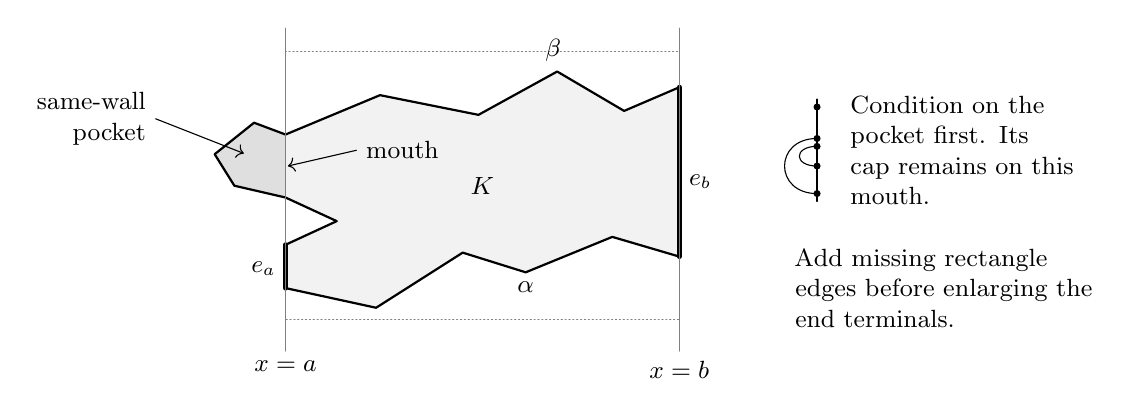
\begin{tikzpicture}[x=1cm,y=1cm,font=\small,line cap=round,line join=round]
  \draw[gray,densely dotted] (0,.25) rectangle (5,3.65);
  \path[fill=gray!10] (0,.65) -- (1.15,.4) -- (2.25,1.1) -- (3.05,.85) -- (4.15,1.3) -- (5,1.05)
    -- (5,3.2) -- (4.3,2.9) -- (3.45,3.4) -- (2.45,2.85) -- (1.2,3.1) -- (0,2.6)
    -- (0,1.8) -- (.65,1.5) -- (0,1.2) -- cycle;
  \path[fill=gray!25] (0,1.8) -- (-.65,1.95) -- (-.9,2.35) -- (-.4,2.75) -- (0,2.6) -- cycle;
  \draw[thick] (0,.65) -- (1.15,.4) -- (2.25,1.1) -- (3.05,.85) -- (4.15,1.3) -- (5,1.05);
  \draw[thick] (0,1.2) -- (.65,1.5) -- (0,1.8) -- (-.65,1.95) -- (-.9,2.35) -- (-.4,2.75)
    -- (0,2.6) -- (1.2,3.1) -- (2.45,2.85) -- (3.45,3.4) -- (4.3,2.9) -- (5,3.2);
  \draw[line width=1.8pt] (0,.65) -- (0,1.2);
  \draw[line width=1.8pt] (5,1.05) -- (5,3.2);
  \draw[densely dashed] (0,1.8) -- (0,2.6);
  \draw[gray] (0,-.15) -- (0,3.95);
  \draw[gray] (5,-.15) -- (5,3.95);
  \node[below] at (0,-.15) {$x=a$};
  \node[below] at (5,-.15) {$x=b$};
  \node[left] at (0,.9) {$e_a$};
  \node[right] at (5,2) {$e_b$};
  \node at (2.5,1.95) {$K$};
  \node[above] at (3.4,3.4) {$\beta$};
  \node[below] at (3.05,.85) {$\alpha$};
  \draw[<-] (-.53,2.36) -- (-1.65,2.8);
  \node[anchor=east,align=right] at (-1.65,2.8) {same-wall\\pocket};
  \draw[<-] (.03,2.2) -- (.9,2.4);
  \node[anchor=west] at (.9,2.4) {mouth};
  \draw (6.75,1.75) -- (6.75,3.05);
  \fill (6.75,1.85) circle (.045);
  \fill (6.75,2.2) circle (.045);
  \fill (6.75,2.45) circle (.045);
  \fill (6.75,2.55) circle (.045);
  \fill (6.75,2.95) circle (.045);
  \draw (6.75,1.85) .. controls (6.2,1.85) and (6.2,2.55) .. (6.75,2.55);
  \draw (6.75,2.2) .. controls (6.45,2.2) and (6.45,2.45) .. (6.75,2.45);
  \node[align=left,anchor=west,text width=3.2cm] at (7.05,2.4)
    {Condition on the pocket first. Its cap remains on this mouth.};
  \node[align=left,anchor=west,text width=4cm] at (6.35,.65)
    {Add missing rectangle edges before enlarging the end terminals.};
\end{tikzpicture}
\caption{A slab core cut from a winding corridor (schematic; lattice steps are suppressed). Consecutive opposite-wall cuts $e_a,e_b$ retain the ends. Same-wall excursions beyond a slab level are pockets, removed along their mouths to obtain $K$. Each pocket induces a separate noncrossing cap on its own mouth. The rectangle comparison preserves these caps while adding missing edges; only afterwards are the contact intervals merged with their respective terminals.}
\label{fig:slab-pockets}
\end{figure}


\smallskip\noindent
\emph{Good slabs and their cost.}
Fix a small number $\tau>0$, say $\tau=1/100$.  Choose $\zeta>0$
sufficiently small compared with $\tau^4$, and subsequently choose a
fixed integer $S_0$ sufficiently large compared with $\zeta^{-1}$ and
all lattice roundoff constants.  Take a maximizing collection for
$V_x$.  Its terms with $s<S_0$ cost at most $O(R^2S_0^4)$, which is
$O(R^4)$ with these fixed choices.  Group the remaining spans by
$h\le s<2h$, where $h=2^kS_0$.  Round the two end levels inward to a
common integer grid of spacing $\lfloor\zeta h\rfloor$, choosing
$a,b$ strictly inside them.  Each moves by at most $\zeta h+1$, so
\[
 b-a\ge s-O(\zeta h+1).
\]
Construct one $J,K,\alpha,\beta$ as above for each chosen passage.
Call it good if
\begin{equation}
 (p_+-p_-)+(P_+-P_-)
 +|\beta(a)_y-\alpha(a)_y|
 +|\beta(b)_y-\alpha(b)_y|\le\zeta h.
 \label{rect:good-slab}
\end{equation}

Members of the maximizing collection may share an end cut.  The chosen
levels $a,b$ lie strictly between each member's own end levels, so its
subquadrilateral $J$ does not use such a common end cut.  Their original
side-wall subarcs have disjoint longitudinal interiors.  Hence the
constructed core interiors are disjoint; any remaining boundary contact
only permits equality in the ordering below.
For a fixed pair $a,b$, the core disks are slab-ordered.  Their
bounding crossings cannot interleave: a slab crossing belonging to one
core would then separate points of the connected interior of another.
Minima, maxima, and the two endpoint heights of ordered disjoint
crossings are ordered as well, with weak inequalities sufficient.
Thus each of the four nonnegative gap sums in
\eqref{rect:good-slab} telescopes to at most $H$, and their total is at
most $4H$.  The number of bad choices at fixed $a,b$ is at most
$4H/(\zeta h)$.  There are $O_\zeta((R/h)^2)$ rounded pairs, so at this
scale there are $O_\zeta((R/h)^3)$ bad choices.  Their contribution to
$V_x$ is $O_\zeta(R^3h)$.  Summing over the dyadic scales $h\le R$
gives $O(R^4)$.

\smallskip\noindent
\emph{Amplification of a good passage.}
For a good passage the height $P_+-p_-$ is at least $b-a-O(1)$.
Otherwise the comparison rectangle \eqref{rect:comparison-box} would
be hard in the sense of \eqref{rect:hard-square}, contradicting the
connection probability at least $1-\epsilon$ in $J$.  Subtracting the
two extrema gaps in \eqref{rect:good-slab} gives the mandatory inner span
\begin{equation}
 T:=P_--p_+\ge s-O(\zeta h+1).
 \label{rect:inner-span}
\end{equation}
Choose integer levels a bounded distance inside $p_+$ and $P_-$.
Every end-to-end path visits both strict sides of each of these levels,
so the level-cut fact gives horizontal transversals.  The span between
two such low and high cuts is $T-O(1)$.

If $T\ge1.05s$, that one horizontal passage already has fourth power
larger than $(1+\gamma)s^4$ for some fixed $\gamma>0$, once $S_0$ is
large.  Otherwise the height and width of \eqref{rect:comparison-box}
are within the aspect-ratio range of Lemma~\ref{rect:corner}.  Every
point of each end interval must be at least $s/16$, for definiteness,
above the lower extreme and below the upper extreme, after increasing
$S_0$ and decreasing $\zeta$ if necessary.  Indeed if one endpoint
interval approaches an extreme more closely, the endpoint gap bound
in \eqref{rect:good-slab} places all contacts on that vertical side
within $s/16+O(\zeta h+1)$ of that extreme.  The comparison box then
has a corner electrode contained in its bottom or top eighth, and
Lemma~\ref{rect:corner} contradicts high connection.

Starting from the longitudinal first end of $J$, consider the earlier
of the selected low and high transversals.  The original end lies in
the central height range just established, while that earlier cut is
near the corresponding extreme.  Choose an intermediate horizontal
integer level between them at distance at least $\tau s$ from the
extreme cut.  The two ends of this first subquadrilateral are on strict
opposite sides of the intermediate level, so it contains a transversal
there.  The resulting extra horizontal passage precedes the low--high
passage and has disjoint longitudinal interior from it.  This works
in either order of the low and high cuts.  Its span is at least
$\tau s$, with bounded roundoff absorbed by the choices of constants.

The two contributions are therefore at least
\[
 \bigl(1-O(\zeta+S_0^{-1})\bigr)^4s^4+\tau^4s^4
 \ge(1+\gamma)s^4
\]
for a fixed $\gamma>0$, by choosing $\zeta$ and then $S_0^{-1}$ small
enough compared with $\tau^4$.  The constructed horizontal passages
are contained in their respective original vertical subquadrilaterals,
so all chosen contributions retain disjoint interiors.

\smallskip\noindent
\emph{Conclusion.}
Combining the good passages and the two error bounds gives
\[
 V_y\ge(1+\gamma)(V_x-C_0R^4).
\]
The same construction with the two coordinate directions exchanged,
and with the original longitudinal wall roles unchanged, gives
\[
 V_x\ge(1+\gamma)(V_y-C_0R^4).
\]
Substitution bounds each variation by a constant multiple of $R^4$.
Together with \eqref{rect:initial-variation}, this proves
\eqref{rect:packing-bound}.
\end{proof}

\subsection{Rectangle crossing bounds}

We now apply the packing lemma. The first half of the contradiction
argument concerns network probabilities in ordinary rectangles. The
second half puts finitely many primal and dual events in one law,
extracts actual crossings, and uses their unexplored sides to obtain
the pure corridor laws required by Lemma~\ref{rect:packing}.

\begin{proposition}[Rectangle RSW for separate electrodes]
\label{prop:rectangle-rsw}
For every fixed $\Lambda\ge1$ there is $c_\Lambda=c_\Lambda(q)>0$
such that
\begin{equation}
 \inf_{\substack{n,w\in\Z_{\ge1}\\w\le\Lambda n}}g_x(w,n)
 \ge c_\Lambda.
 \label{rect:rsw}
\end{equation}
The same holds after translation, lattice rotation, reflection, or
translation to the shifted dual square lattice.  All probabilities
refer to separate full crossing electrodes with no other wires.
\end{proposition}

\begin{proof}
Suppose otherwise.  Lemma~\ref{rect:square} and positivity on each
fixed finite graph give a sequence with
\begin{equation}
 n\longrightarrow\infty,\qquad n\le W_n\le\Lambda n,
 \qquad g_x(W_n,n)\longrightarrow0.
 \label{rect:degeneration}
\end{equation}
All limits in $n$ below are along \eqref{rect:degeneration}. Every
macroscopic separation, relative interval width, and bulk clearance
invoked in a convergence assertion is fixed and positive before taking
that limit. These constants may depend
on the finite number of chords to be used, but not on $n$. A convergence
assertion for a stated class of rectangles and intervals means that it
holds for every sequence of integer choices satisfying those same fixed
conditions. Equivalently, the convergence is uniform over that class:
a failure of uniformity would select a violating sequence, to which
the same subsequence contradiction applies.

\smallskip\noindent
\emph{Separated arches vanish.}
For each fixed $\sigma>0$, consider ordinary rectangles with positive
integer width and height at most $n/8$, and two nonempty top intervals
whose horizontal separation is at least $\sigma n$. Their network
probability tends to zero uniformly over these choices. Otherwise, after taking a
subsequence, there is such a chord bounded below.  Subdivide both
intervals into a bounded number of subintervals of diameter at most
$\sigma n/10+O(1)$.  By \eqref{rect:subadditivity}, a pair of these localized
intervals still has a chord bounded below.  Translate copies of its
rectangle along the top of $R_{W_n,n}$, starting at the left side, with
integer displacement close to half the separation of the two localized
centers.  Consecutive chords interlace strictly; they retain their lower
bounds by Lemma~\ref{rect:extension}.  Continue while the rectangles
fit.  A bounded number of applications of
\eqref{rect:interlacing}, depending only on $\sigma,\Lambda$, joins the
first endpoint to the last far endpoint with probability bounded below.
The first lies within $n/8$ of the left side and the last within
$n/8+n/16+O(1)$ of the right side.

A square of side $\lfloor n/2\rfloor$ at the upper-left corner has a
chord from its left side to the far half of its top side bounded below:
reflection and subadditivity give the half-side crossing, then
interlacing with an opposite full square crossing gives the stated
chord.  The analogous upper-right square gives the other end chord.
They interlace the long top chord to the full left and right sides.
This contradicts \eqref{rect:degeneration}.  Reflection gives the same
vanishing statement for bottom arches.  Translation gives it on the
shifted grid as well.

\smallskip\noindent
\emph{Only aligned chords can survive.}
Fix $0<c_-\le c_+\le1/8$ and $0<\theta<1/2$. For integer square sides
$c_-n\le h\le c_+n$, a top electrode contained in
$[0,(1/2-\theta)h]$ or in $[(1/2+\theta)h,h]$ connects to the full
bottom side with probability tending uniformly to zero.
If not, reflect that electrode and its chord across the vertical center
line.  Interlace the two top--bottom chords separately with the
full left--right square crossing, whose probability is bounded below.
This yields chords from the left top portion to the right side and
from the right top portion to the left side.  Interlacing them gives
a separated same-top arch, contradicting the preceding paragraph.
The corresponding off-center bottom chords also vanish.

Decompose each of the top and bottom sides into its two off-center
portions and the central interval
$[(1/2-\theta)h,(1/2+\theta)h]$, with endpoints rounded to lattice
vertices. The full
vertical crossing has a uniform lower bound.  Subadditivity twice,
and the vanishing just proved, therefore give a positive lower bound
for the chord between the two central neighborhoods.

Now use an integer strip of height $h$ and width $\ell=4h+O(1)$, with
the bound in $O(1)$ fixed,
$h/n$ bounded above and below by fixed positive constants and both
dimensions at most $n/8$. Translated squares give bounded-below chords
between aligned top and bottom patches of fixed positive relative width.
Their centers may vary provided their distances from the vertical ends
are at least $(1/2+\eta)h$ for a fixed $\eta>0$.

In this strip, consider boundary electrodes lying entirely to the left
and right, respectively, of a horizontal gap. Suppose that the gap
contains centers $c_1<c_2$ whose distances from its endpoints and from
each other are at least $\eta h$, and whose distances from the vertical
strip ends are at least $(1/2+\eta)h$, for some fixed $\eta>0$.
The connection probability of those electrodes tends uniformly to zero.
Choose the aligned patches at these centers with length
$\eta h/2+O(1)$ after lattice rounding, so that the two patches are disjoint and
remain in the gap. Interlace a hypothetical
bounded-below chord with the aligned vertical chord at the first
center, joining that top patch to the right electrode, and with the
aligned chord at the second center, joining that top patch to the left
electrode.  The resulting chords interlace to give a forbidden
separated same-top arch.

\smallskip\noindent
\emph{Aligned short electrodes are crossed with probability tending
to one.}
Fix $\theta,\eta>0$ and equal aligned intervals on the top and bottom
of this strip, each of length at least $\theta h$ and contained between
horizontal coordinates $(1/2+\eta)h$ and $\ell-(1/2+\eta)h$.
Contract their boundary edges.
The complementary dual crossing is between the exterior arcs going
around the left and right ends.  Split the corresponding exterior
hub into two hubs.  This costs only a bounded density factor.  Absorb
all adjacent contact vertices into their respective hubs, which cannot
decrease the network probability by terminal monotonicity. The result is an
ordinary interior cell rectangle with two separately wired boundary
electrodes whose horizontal coordinates are separated by the gap
between the endpoints of the original intervals. This gap contains
two centers satisfying the preceding fixed-clearance conditions, with
constants depending only on $\theta,\eta$. The preceding vanishing
argument, on the shifted grid and with bounded lattice roundoff,
applies to this network.  Thus the complementary dual probability
tends to zero, and the original aligned crossing tends to one.
Smaller aligned subintervals of any fixed positive relative width are
covered by the same argument.

\smallskip\noindent
\emph{Many alternating network crossings.}
The preceding steps have shown that every fixed aligned pair of short
intervals in the indicated strip is crossed with probability tending
to one. We next arrange finitely many such primal and dual crossings
in a common law. Their simultaneous success will use a union bound;
no correlation inequality between these events is needed.

For definiteness take $h=\lfloor n/64\rfloor$ and strip width $4h$.
Choose an arbitrarily large but fixed finite ordered list of disjoint
small interval labels in a central bulk part of the top side, and
matching labels in the same order on the bottom.  On the primal graph
wire the odd intervals, each separately, by contracting their boundary
edge runs.  Leave no other primal wires.  Round the runs so that each
intervening even interval retains an uncontracted boundary-edge stretch
of fixed positive relative width.  Only interior labels with neighboring
buffers will be used.

Every desired odd top--bottom network connection tends to one.  This
follows first in the pure two-electrode graph by the aligned estimate,
then in the multiwire graph by adding the other disjoint interval caps
cofacially with its test edge.  The deletion order is the exposed
boundary face expansion used in Lemma~\ref{rect:extension}.

The dual consists of the cell grid and a common outer hub with
stochastic spokes dual to all uncontracted boundary edges.  Split this
hub into separate hubs for the maximal complementary intervals.  Since
the number of intervals is fixed, the density change is bounded by a
fixed power of $q^{-1}$.  We claim that each desired even top--bottom
connection in this split network also tends to one, despite the finite
spoke odds.

Retain first only the two spoke patches over smaller aligned intervals.
Fix a deterministic bottom subinterval wire in that range.  For any
fixed integer $k$, choose $k$ disjoint smaller top patches aligned
within it.  Each is connected to the bottom wire with probability
tending to one by the pure estimate and terminal enlargement.  In the
single rooted-multiset law based at the collapsed bottom electrode,
all $k$ patches are therefore hit with probability tending to one.
Their union has multiplicity at least $k$ on that event.  Formula
\eqref{rect:spokes} gives lower limit at least $1-(1+v)^{-k}$ for the
finite top-spoke connection.  Since $k$ is arbitrary, this probability
tends to one.  Now keep this finite top-spoke graph as the base rooted
at its hub.  Apply the same argument to $k$ disjoint deterministic
bottom subintervals, using the conclusion just established for each
of them.  This makes the bottom spokes finite as well, still with
connection tending to one.  The order of limits is first $n\to\infty$
for fixed $k$, then $k\to\infty$.

Extra spokes at the tested hubs cannot decrease connection.  Spokes of
each other hub occupy its own exposed boundary interval and can be
removed by exterior face expansion from the test-edge faces; reversing
this removal does not decrease the tested connection.  Thus the desired even
events tend to one in the full split dual network.  The bounded
hub-joining density transfers them back to the common original law.
Their event definition still uses only the individual split-hub
shortcuts, not the common hub as a path shortcut.

\smallskip\noindent
\emph{From networks to physical crossings.}
All these finitely many primal and dual successes coexist with
probability tending to one.  Draw shortcuts narrowly along their
separate boundary intervals, including dual spokes through the
appropriate boundary-edge midpoints.  Complementary primal and dual
states prevent crossings of opposite-color open paths. For topology
only, place the rectangle and all narrow caps inside a slightly enlarged
disk, and join each designated terminal to a distinct point on its
boundary by outward spokes, preserving the order of the terminal intervals.
For a dual event, the shortcuts here are those of its individual
split hubs, although its edge state is now sampled in the common law.

For each network success, choose a simple witness in this enlarged
disk, with the narrow cap shortcuts included as edges. Its only
contacts with the enlarged boundary are its prescribed top and bottom
endpoints, so it is a crosscut even if it uses another same-color cap
along the way. Opposite-color witnesses are disjoint: their physical
edges cannot cross, and their cap shortcuts and outward spokes occupy
disjoint boundary intervals.

Fix a successful interior label whose two opposite-color neighbors
also succeed. The target crosscut places the endpoints of one neighbor
on one side and those of the other neighbor on the other side.
Their witnesses cannot cross the target, so they lie on those
respective sides and are disjoint from each other. The region between
them meets the top and bottom boundary exactly between the neighboring
labels. Every other same-color cap lies outside that region: its narrow
connection to its own boundary interval is disjoint from the two
neighbors. The target witness therefore cannot use another same-color
wire or hub. Its segment from the last departure from its initial
terminal to the first subsequent arrival at its final terminal is therefore an
actual physical crossing between its labeled intervals.
For a dual label, the crossing retains its initial and final stochastic
boundary spokes and an ordinary cell path, with no intermediate hub
jump. This proves simultaneous physical success for the slightly
smaller range of interior labels that has all required buffers.

\smallskip\noindent
\emph{Uninspected high corridors.}
Select many odd interior labels spaced by at least four.  For each
selected $i$, expose a physical dual crossing for label $i-1$ from
its left side, and one for label $i+1$ from its right side.  The
search uses the physical cell graph with its available boundary
half-extensions at that pair of intervals and fictitious always-open
terminal stars confined to their outer caps. Seed the complementary-face
search at the corresponding exterior side. Query an edge only from a reached face, and advance to the
opposite face only when its physical bond in the path color is closed.
On crossing success this exploration stays outside
every blocking terminal path.  Setting all unqueried edges to the
nonpath state still leaves a path, by the plane path--cut alternative,
so choose a simple witness measurably from the exposed edges.  No
edge with interior on its other side was queried.  The ordered
boundary spokes preserve this property at the endpoints.  Stop each
wall at the physical rectangle boundary-edge midpoint.

Let $\mathcal R_i$ be the combined record of the two searches, including
the queried edge states and the chosen walls. Let $E_i$ be the event,
determined by this record, that both searches succeed with disjoint
walls in the proper order. The simultaneous physical crossings,
including the odd target path separating its two neighbors, imply
$\PP(E_i)\to1$.

Fix a value of $\mathcal R_i$ in $E_i$. Every fully contained primal
edge between the walls, other than the deterministic boundary edges
along the target wires, is uninspected, and every primal edge crossing
a wall is closed. The top and bottom intervals contain exactly the
two target primal wires: the wall endpoints lie in the flanking
uncontracted intervals, and no exterior tie enters the corridor.
Omit the boundary edges along the target wires, which are independent
loops after contraction, and let $G_i$ be the remaining contained-edge
graph. Finite conditioning now gives exactly the FK law on $G_i$ with
the two target electrodes separately wired. Indeed the queried closed
edges separate the corridor from the exterior across both walls, and
the original boundary partition has
no other class meeting the corridor; integrating the exterior therefore
introduces no additional identification. Restoring the omitted loops
with their independent ordinary law changes no crossing probability.

Let $g_i$ be the pure corridor probability from
Definition~\ref{rect:corridor-definition}, measurable from
$\mathcal R_i$, and let $T_i$ be the target's actual physical crossing
event in the original strip. On $E_i$, such a path cannot cross either
dual wall, so it is contained in the corridor. The preceding conditional
law and the two-wire path equivalence give
$\PP(T_i\mid\mathcal R_i)=g_i$ on $E_i$. Since $\PP(T_i)\to1$,
\begin{equation}
 \EE\bigl[(1-g_i)\one_{E_i}\bigr]
   =\PP(E_i\cap T_i^c)\longrightarrow0.
 \label{rect:conditional-high}
\end{equation}
Markov's inequality gives $g_i\ge1-\epsilon$ on $E_i$ with probability
tending to one.  Perform these searches on the same configuration for
each of the finitely many selected indices.  Equation
\eqref{rect:conditional-high} was applied separately to each search;
no joint unexplored independence is required.  With probability tending
to one all the high-corridor conclusions hold together with the
intervening physical crossings.  In particular intervening odd primal
crossings separate different pairs of dual walls, so the resulting
corridors have disjoint closures.

The strip aspect ratio is fixed.  Choose the finite number of selected
labels larger than the constant allowed by
Lemma~\ref{rect:packing}.  For large $n$, any realization with all the
preceding properties violates \eqref{rect:packing-bound}.  Such
realizations have probability tending to one, a contradiction.  This
proves \eqref{rect:rsw}.
\end{proof}

\subsection{One-sided boundary density}

The rectangle crossing bound is now proved. For the later sector and
disk arguments we also need to control partition-function gains when
a distant boundary wire is changed. These comparisons use
Section~\ref{sec:pressure} directly, independently of the rectangle
crossing proposition. We return to arbitrary positive
edge odds on a finite ordinary plane graph $H$ in a closed disk, with
no initial wires. Lemma~\ref{lem:one-sided-density} bounds that interaction
by the pure connection probability; the final subsection replaces full
wires by arbitrary separate planar caps.
For a nonempty vertex set $D$, let $k_D$ count physical open components
meeting $D$, and put
\[
 K_H(D)=\log\EE_H t^{k_D},\qquad
 \Delta_H(S,W)=K_H(S)+K_H(W)-K_H(S\cup W).
\]
The coverage representation from Lemma~\ref{lem:rooted} gives
$\Delta_H(S,W)\ge0$.  Denote the full wire on $D$ by $F_D$.
For a partition $X$ let $Z_X$ be the partition function on the original
edge sets with weight $v_Aq^{k_{H/X}(A)}$, retaining any quotient loops;
write $Z=Z_\varnothing$.

\begin{lemma}[Auxiliary-link gain in an exposed face]
\label{rect:face-gain}
Let $e$ be a physical edge bordering a face $F$ of a finite plane
graph.  Let $T$ be a finite noncrossing collection of auxiliary links
whose endpoints are graph vertices and whose interiors lie in $F$.
At fixed positive auxiliary odds, the partition-function gain from
adding all links of $T$ is nonincreasing in the odds of $e$.
The conclusion passes to a prescribed partition obtained by contracting
the links.  Repeated boundary vertices, auxiliary loops, and redundant
links are allowed in the corresponding plane minors.
\end{lemma}

\begin{proof}
In the drawing with all links present, start from a face sector incident
to $e$.  The dual adjacency graph of regions into which the links cut
$F$ is connected, since the original face $F$ was connected.  Remove
a frontier auxiliary link to expand the reached $e$-face and repeat,
also removing auxiliary links with that reached face on both sides.
Eventually every link is removed.  Reverse this order.  At each
addition, the link and $e$ are cofacial in the graph including the new
link.  Cofacial Rayleigh implies that its log partition gain, integrated
from zero to its specified odds, is nonincreasing in the odds of $e$.
Sum these log gains.  The removal order may be chosen separately for
each physical edge and each background graph.

For auxiliary odds $\lambda_f$, divide the augmented partition function
by $\prod_{f\in T}\lambda_f$ and send every $\lambda_f$ to infinity.
Only the term with all auxiliary links open survives, and it is exactly
the contracted-graph partition function.  Retaining the same links and
normalizing product after any physical minor handles links that become
loops or redundant.  This proves the limit statement as well.
\end{proof}

\begin{lemma}[One-sided small-network density]
\label{lem:one-sided-density}
Let $S,W$ be disjoint nonempty vertex sets on two disjoint accessible
boundary arcs of $H$.  Put $p=g_H(S,W)$ and suppose $tp<1$.
For every noncrossing partition $X$ supported on $S$,
\begin{equation}
 0\le \log\frac{Z_XZ_{F_W}}{Z_{X,F_W}Z}
 \le\Delta_H(S,W)
 \le\log\left(1+\frac{(t-1)p}{1-tp}\right).
 \label{rect:one-sided-density}
\end{equation}
\end{lemma}

\begin{proof}
There are three steps. A component exploration bounds the number of
physical crossings by a geometric tail. A covariance inequality turns
that tail into the asserted upper bound on $\Delta_H(S,W)$. Finally,
an exact full-wire identity and cofacial comparison give the two bounds
for an arbitrary partition $X$.

\paragraph{A geometric tail for crossing components.}
In either the separately
$S,W$-wired law or their jointly wired law, let $L$ be the number of
distinct physical components meeting both sets, before any identification.
Then
\begin{equation}
 \PP(L\ge j)\le p^j\qquad(j\ge1).
 \label{rect:component-tail}
\end{equation}

Explore whole physical components from the vertices of $W$ in their
linear boundary order, skipping vertices already visited and never
following a wire as a physical edge.  Component searches test every
incident physical edge.  After a prefix, possibly stopped immediately
after a crossing component, let $U$ be the explored union.  Every
vertex of $U$ has a path in $U$ to that prefix.  On $H-U$, component
counting leaves precisely the full remaining $W$ and $S$ wires,
possibly joined, and no other ties.  Joining them multiplies the
weight of separation by $t$ relative to connection; hence the
conditional probability of another crossing component is at most
\[
 g_{H-U}(W\setminus U,S\setminus U),
\]
interpreted as zero if either set is empty.

This last quantity is at most $p$.  To verify the comparison rather
than invoke arbitrary boundary monotonicity, keep all vertices of $H$
temporarily.  Draw narrow exterior chains along $W$ and $S$, and a
test edge from the first $W$ vertex to the facing endpoint of $S$
across the intervening gap.  Starting in its gap-side face, delete
the physical fan of the first $W$ vertex.  This opens the inner lip
of the narrowly exterior chain up to the next prefix vertex.  The
thin sector between a chain link and its underlying boundary interval
contains no physical edge or other auxiliary link, so the exposed
face can advance successively along the entire explored prefix.
Continue into $U$ along paths to that prefix: deleting an onward
physical edge exposes a sector at the next vertex, from which its
whole physical fan can be deleted in order.  At a boundary vertex
the physical fan is inward and contains no interspersed auxiliary
links.  No chain link needs to be removed.  Thus every removed
physical edge is cofacial with the test edge at its removal.

At finite positive chain odds, cofacial Rayleigh makes connection
nonincreasing under these deletions.  Send the chain odds to infinity.
This comparison starts from the original \emph{separate}-wire graph,
not from the conditional graph in which a previous crossing may have
joined the electrodes.  Every physical edge touching $U$ has been
deleted, and the retained $W$ and $S$ chains have disjoint vertex sets;
they cannot create a tie between the two sides.  After contracting
each chain, a test endpoint originally in $U$ is the same quotient
vertex as any surviving vertex of its own electrode.  Use such
surviving representatives on both sides; the case of an empty surviving
electrode was already assigned probability zero.  Isolated vertices
off the two chains factor out.  Thus the remaining test is exactly the
separate two-electrode problem on $H-U$, irrespective of whether the
earlier conditional problem had joined wires.
This proves the comparison.  Each successive exploration success
therefore has conditional probability at most $p$, and iteration
proves \eqref{rect:component-tail}, including for the initially
joined law.

\paragraph{From the tail to the full-wire interaction.}
We need the rank-factor covariance inequality
\begin{equation}
 \EE_H t^{k_S+k_W}\ge
 \EE_H t^{k_S}\,\EE_H t^{k_W}.
 \label{rect:rank-covariance}
\end{equation}
Here is its finite-graph proof.  More generally consider two full-wire
rank factors $t^{k_D-1}$, where each set can be joined by links inside
one common physical face; the two prospective drawings may be
considered separately.  The invariant under minors is the inherited
auxiliary drawings in one common physical face, not the original
disjoint-arc description: image electrodes may overlap or shrink.
Induct on the number of physical edges.
Choose an edge $e$ bordering that face.  For either prospective wire,
its expected rank factor conditional on $e$ open is no greater than
conditional on $e$ closed.  Draw its auxiliary links at finite odds,
peel them from a face sector incident to $e$, and add them back in
reverse order.  At each addition the new link and $e$ are cofacial in
the graph containing both, as in Lemma~\ref{rect:face-gain}.
Cofacial Rayleigh says that its
partition-function gain is nonincreasing with the odds of $e$.
Multiply these gains and take the full-wire limit.  This proves the
asserted conditional-mean inequality.

In each of deletion and contraction of a nonloop $e$, the prospective
wire drawings remain in the image of the same face.  The rank factors
restrict exactly to the corresponding rank factors of the minor,
with coincident marked vertices identified.  Thus the conditional
covariances are nonnegative by induction.  The additional term in
the total-covariance formula is nonnegative because both conditional
mean differences have the same sign.  A loop changes neither rank
factor and can be omitted; if no physical edge remains, the factors
are deterministic.  This completes the induction.  To take an
auxiliary-wire limit without ambiguity, divide the augmented
partition function by the product of all auxiliary odds before
sending them to infinity.  The surviving all-open term is exactly
the contracted-graph partition function, even when some links have
become redundant or loops in a minor.  Since $S,W$ are on the same
outer face, the general inequality yields
\eqref{rect:rank-covariance}.

Every physical component meeting both $S,W$ is counted twice on the
left and once on the union, so
$L=k_S+k_W-k_{S\cup W}$.  Equation
\eqref{rect:rank-covariance} therefore gives
\begin{equation}
 e^{\Delta_H(S,W)}
 \le\frac{\EE_H t^{k_S+k_W}}{\EE_H t^{k_{S\cup W}}}
 =\EE_{H/F_{S\cup W}}t^L.
 \label{rect:interaction-moment}
\end{equation}
The normalization for full wiring is $t^{k_{S\cup W}-1}$; its
constant factor cancels in this expectation.  From
\eqref{rect:component-tail},
\[
 \EE t^L
 =1+(t-1)\sum_{j\ge1}t^{j-1}\PP(L\ge j)
 \le1+\frac{(t-1)p}{1-tp}.
\]
This proves the final upper bound in
\eqref{rect:one-sided-density}.

\paragraph{An arbitrary partition on the first end.}
Let $S'$ be the image of $S$ in $H/X$.  A full-$D$ log gain is
$K_H(D)-\log t$, and the full $S$ and full $S\cup W$ wires both
subsume $X$.  Writing these gains out gives the exact identity
\begin{equation}
 \log\frac{Z_XZ_{F_W}}{Z_{X,F_W}Z}
 =\Delta_H(S,W)-\Delta_{H/X}(S',W).
 \label{rect:interaction-difference}
\end{equation}
Coverage positivity in the quotient proves the middle upper bound.

For the lower bound draw the noncrossing $X$ links and a full-$W$
chain in separate exterior caps facing the main exterior.  Peel the
$X$ links from that main face and add them in reverse order.  For
each link being added, the $W$ links may likewise be ordered by
reverse peeling from its incident outer-face sector.  Each compared
pair is then cofacial at the moment of comparison.  Cofacial Rayleigh
does not increase the $W$ partition gain when the $X$ links are present.
Integrate at finite odds, multiply the successive gains, and take
the wire limits with the preceding normalization.  Thus
$Z_{X,F_W}/Z_X\le Z_{F_W}/Z$, proving nonnegativity and completing
the lemma.
\end{proof}

\begin{corollary}[A marginal comparison]
\label{rect:one-sided-marginal}
Suppose that an exterior configuration meets a collar only along $S$
and induces there an arbitrary noncrossing partition $X$, while $W$
is free.  If the collar's pure probability $g_H(S,W)$ tends to zero,
adding the full wire at $W$ changes the exterior marginal by a density
tending uniformly to one.
\end{corollary}

\begin{proof}
Conditional component counting makes the unnormalized density factor
$Z_{X,F_W}/Z_X$.  By Lemma~\ref{lem:one-sided-density} its ratio to
the fixed factor $Z_{F_W}/Z$ lies between $e^{-\varepsilon_p}$ and
one, where $\varepsilon_p\to0$.  Division by its average gives a
normalized density between $e^{-\varepsilon_p}$ and
$e^{\varepsilon_p}$, uniformly in $X$.
\end{proof}

\subsection{No-hit comparison and arbitrary separate caps}

The next result uses actual physical components throughout.  Neither
the event being compared nor its exploration is allowed to traverse a
boundary identification as a path edge.

\begin{lemma}[End-cap no-hit comparison]
\label{lem:no-hit}
Let $H$ be an ordinary finite plane graph in a closed disk, with
nonempty vertex sets $W,S$ on disjoint accessible boundary arcs and
no preexisting ties.  Let $X$ be a noncrossing partition on $W$ and
$Y$ one on $S$.  Adding $Y$ to the $X$-law does not increase the probability
of an actual physical $W$--$S$ crossing.  Adding $X$ alone to the
blank law also does not increase that probability.
\end{lemma}

\begin{proof}
Relative to the $X$-law, the extra partition gain is the nonnegative
random weight
\[
 f(A)=q^{k_{H/(X,Y)}(A)-k_{H/X}(A)},
 \qquad \EE_{H/X}f=\frac{Z_{X,Y}}{Z_X}.
\]
On no actual crossing, explore all complete physical open components
touching $W$, without using ties as physical links.  Their union $U$
contains $W$ and avoids $S$.  All edges from $U$ to its complement
are closed.  Every $X$ tie is contained in $U$, and conditional
component counting shows that the conditional mean of $f$ is exactly
the $Y$-partition gain in the ordinary graph $H-U$.

This gain is at least the unconditional mean of $f$ in the $X$-law.
Draw all prospective cap links.  With $Y$ temporarily absent in
describing faces, delete the $X$ links in an order expanding the
exterior face from the $S$ cap.  Then peel all physical edges touching
$U$ from this exposed face: start at $W$, delete its inward fans, and
continue along paths in each explored component to the vertices
reached.  All those components touch $W$, and no $S$ vertex is removed.
At each deleted edge $e$, the $Y$ log partition gain cannot decrease.
For a precise finite-odds comparison, peel the prospective $Y$ links
from the face sector incident to $e$ through their cap, then add them
in reverse order.  Each newly added link is cofacial with $e$ in
the graph containing both.  Cofacial Rayleigh makes its log gain
nonincreasing with the odds of $e$.  Decrease those odds to zero and
repeat.  The order for $Y$ may be chosen anew for each deleted edge;
there is no claim that all nested cap links are simultaneously
cofacial.  Finally send auxiliary odds to infinity after dividing
out their common leading product.  During physical peeling retain
the vertices of $U$ temporarily.  Since $U$ avoids all $Y$ endpoints,
its isolated vertices contribute the same factor $q^{|U|}$ to the
ordinary gain's numerator and denominator and then cancel.  This proves
the asserted comparison with
$H-U$.

Consequently
\[
 \EE_{H/X}[f\mid\text{no hit}]\ge\EE_{H/X}f.
\]
Tilting by $f$ does not decrease the no-hit probability, and hence does not increase
the physical crossing probability.  To compare the $X$-law with
the blank law, use the same argument with the two ends exchanged
and with the initial partition empty.
\end{proof}

\begin{lemma}[Decoupling of separate cap gains]
\label{lem:separate-caps}
In the setting of Lemma~\ref{lem:no-hit}, put
$b_H=\PP_H(W\leftrightarrow S)$ for the actual crossing probability
in the blank law.  Then
\begin{equation}
 (1-b_H)\frac{Z_Y}{Z}
 \le\frac{Z_{X,Y}}{Z_X}
 \le\frac{Z_Y}{Z}.
 \label{rect:separate-cap-gains}
\end{equation}
In particular, when $b_H\to0$, the gain of an arbitrary partition on
one end is asymptotically unchanged, uniformly, by an arbitrary
noncrossing partition on the other end.
\end{lemma}

\begin{proof}
The upper bound is the finite-odds cofacial cap comparison used at
the end of Lemma~\ref{lem:one-sided-density}, now with arbitrary
noncrossing $Y$ in place of a full wire.  Peel the cap links from
the main exterior and add them in reverse order, ordering the
opposite cap as necessary for each comparison.  Each pair is
cofacial when Rayleigh is applied.  Integrating and taking the
normalized contraction limits gives the upper bound.

For the lower bound, use the no-hit component exploration from
Lemma~\ref{lem:no-hit} in the $X$-law.  On no actual hit its
conditional $Y$ gain is the blank $Y$ gain in $H-U$.  By just the
physical-edge peeling part of that proof, comparing this time
against the empty base cap, that gain is at least $Z_Y/Z$.
Lemma~\ref{lem:no-hit} gives no-hit probability at least $1-b_H$.
Keeping only this nonnegative contribution to the mean of $f$ yields
\[
 \frac{Z_{X,Y}}{Z_X}=\EE_{H/X}f
 \ge\PP_{H/X}(\text{no hit})\frac{Z_Y}{Z}
 \ge(1-b_H)\frac{Z_Y}{Z}.
\]
This is the claimed inequality.
\end{proof}

\begin{remark}[Scope of the comparisons]
\label{rect:scope}
The two density statements require separate accessible end arcs with
all physical incidences on the disk side.  The last two lemmas start
with no obstructing preexisting ties.  Neither their proofs nor
Proposition~\ref{prop:rectangle-rsw} assert stochastic monotonicity
for arbitrary boundary conditions, or comparison between arbitrary
partitions on noncofacial rims.  These restrictions will be retained
when the estimates are used in more complicated domains.
\end{remark}

\section{Sector decay and bounded annular densities}
\label{sec:sectors}

Throughout this Section, $q\in(0,1)$ is fixed and
\[
 t=q^{-1},\qquad u=1-q,\qquad v=\sqrt q.
\]
Ordinary grid edges have odds $v$.  Constants may depend on $q$ and
on each fixed geometric parameter.  In particular, no constant below
is asserted to be uniform as $q$ approaches an endpoint of $(0,1)$.
A boundary identification changes component counting but is never an
edge of an \emph{actual} path.  Boundary incidences at the two banks of
a cut remain distinct.

We first establish decay in a disk sector, for a two-terminal network
test and then for an actual path in the blank law.  The second part of
the section uses this decay to bound the interaction between the two
rims of an ordinary annulus.  It follows the connected supports of the
site-pressure expansion: a diverging interaction would force these
supports to fill every clear bulk region, while a free wall or a
measured path makes that impossible.  These estimates supply the regular
collars used in the irregular-disk arguments of Section~\ref{sec:disks}.
Throughout, boundary comparisons retain their stated cap restrictions.

\subsection{Straight-wall sectors and their dual networks}
\label{sector:radial-setup}

Fix an integer $k\geq1$.  Take $k$ consecutive copies of a coordinate
quadrant, glue their intervening radial sides in order, and do not identify
the first and last sides.  All the constructions in this subsection take
place on this noncyclic angular cover.  For integers $1\leq r<R$, let
$H_k(r,R)$ be the mesh-one graph between the sup-norm levels $r$ and $R$,
including all vertices and edges in the closed region.  Its two level
arcs are denoted by $S_r$ and $S_R$, and its two remaining boundary arcs
are its \emph{flanks}.  The underlying surface is a closed disk.  For
$k=4$ the two banks of the coordinate slit remain distinct; the same
convention applies when $k>4$.  Thus local square-grid coordinates are
used on an abstract disk, not on a cyclically identified annulus.
Set
\begin{equation}\label{sector:Q-definition}
 Q_k(r,R)=g_{H_k(r,R)}(S_r,S_R),
 \qquad
 \mathcal H(p)=\frac{1-p}{1-up}.
\end{equation}
The two level arcs in this definition are wired separately.  Constants
below may depend on the fixed $k$ and on $q$, but not on the radii.

\begin{proposition}[Radial network decay]\label{prop:sector-network}
For every fixed finite $k\geq1$, every lattice rotation or reflection of
the construction, and every translate of its center to a lattice site,
\begin{equation}\label{sector:network-decay}
 \lim_{L\to\infty}\ \sup_{\substack{1\leq r<R\\R/r\geq L}}
 Q_k(r,R)=0.
\end{equation}
This is a separately wired two-terminal network statement on the
noncyclic disk sector.
\end{proposition}

We first record the geometry and duality needed for its proof.  Let
$C_k(r,R)$ be the cell-center graph of the sector: its vertices are the
centers of its square cells, and neighbors are joined across interior
edges.  To this graph add two distinct hubs, one for each flank, with an
odds-$v$ spoke dual to every edge on that flank.  Denote the connection
probability of the two hubs by $P_k^*(r,R)$.

\begin{lemma}[Exact split-hub duality]\label{sector:duality}
One has
\begin{equation}\label{sector:duality-equation}
 P_k^*(r,R)=\mathcal H(Q_k(r,R)),\qquad
 \mathcal H(\mathcal H(p))=p.
\end{equation}
The same assertion holds for a cell-center passage between two
concentric layer cuts, using its own cell dual and its two flank hubs.
\end{lemma}

\begin{proof}
Contract each level arc separately.  Edges along a contracted arc are
loops and contribute factors independent of the remaining configuration,
so they may be omitted.  The ordinary plane dual has precisely the
interior cell graph just described, with a \emph{single} exterior hub
carrying the spokes from both flanks.  Its odds are $q/v=v$.
Euler's formula gives the FK dual law with these odds.  The disk
path--cut alternative identifies absence of the primal level-to-level
connection with an open dual traversal from one flank to the other
through the cells, without using the common hub as a shortcut.

Split the common hub into its two flank hubs and let $p$ be their
connection probability in the split law.  Joining the hubs changes the
component count by one on separation and by zero on connection.
Consequently the joined law gives the traversal event probability
\[
 \frac{p}{p+t(1-p)}=\frac{q p}{1-up}.
\]
This is $1-Q_k(r,R)$.  Solving for either probability proves
\eqref{sector:duality-equation}; direct substitution proves that
$\mathcal H$ is involutive.  This reasoning uses only the disk boundary
order and the square-cell incidence structure, so applies to the
cell-center passage as well.  No Euclidean identification across a slit
or between different sheets of the angular cover is made.
\end{proof}

The next lemma turns rectangle crossings into a connection along a
boundary route.  It will be used twice: along the outer rim to bound the
split-dual test, and around an end gap to extend a measured actual arm.
The latter use requires the reflex-corner case as well as convex corners.

\begin{lemma}[Boundary chords along a rectilinear route]
\label{sector:blank-boundary-chain}
Consider a square-grid disk graph, in ordinary coordinates or on a
noncyclic angular cover, with two accessible boundary intervals $I$ and
$J$, separately wired for the test and with no other ties.  Suppose that
a boundary route from $I$ to $J$
has a bounded number of straight portions of comparable macroscopic
length, positive inward clearance of comparable size along each
portion, and right-angle convex or reflex corners.  The fitting inward
rectangular neighborhoods along straight portions and inward square
neighborhoods at convex corners must contain every grid vertex and
nearest-neighbor edge of their closed regions, including boundary edges,
with ordinary odds $v=\sqrt q$.  At a reflex corner, require the same
complete ordinary grid on a fitting closed square of comparable size
with its exterior quadrant removed.  Suppose also that $I$ and $J$
have positive length on this same scale.  Then
\[
 g(I,J)\ge c>0,
\]
where $c$ depends only on $q$, the bound on the number of straight
portions, and the fixed length and clearance ratios.
The estimate remains valid after a cofacial extension for
which every added edge is accessible from a test-edge face by
crossing only added edges.
\end{lemma}

\begin{proof}
All the comparisons here use auxiliary interval chains in narrow
exterior caps and an exterior terminal test edge.  When a rectangle
is flush to a continuous exposed boundary stretch, every unwanted
edge can be reached from a test-edge face across only unwanted edges.
Successive face expansion therefore peels the unwanted edges, and
cofacial Rayleigh gives the rectangle-to-disk comparison in the
required direction.  Interval caps can be chosen with no physical
edge in their thin pockets, so they do not obstruct the peeling.

Proposition~\ref{prop:rectangle-rsw} first gives chords from a fixed
positive-length patch to the opposite side of a fitting subrectangle.
For two patches on adjacent sides, the two patch-to-opposite-side
chords interlace.  Lemma~\ref{lem:interlacing} therefore gives a
positive lower bound for their connection.  For two patches on the
same side, first connect each toward the opposite side.  Interlace
each of these chords with a transverse rectangle crossing, choosing
the right-hand endpoint for the left patch and the left-hand endpoint
for the right patch.  The resulting two chords again interlace and
connect the original patches.  When two input full-side electrodes meet
at a corner, use
Corollary~\ref{rect:interlacing-abutments}; the two patches to be
connected are disjoint and stay away from that corner.  All rectangles
have fixed aspect ratios and positive relative patch sizes.  At a convex
corner the same adjacent-side construction takes place in an inward square.

Here is the corresponding construction at a reflex corner.  In local
coordinates take $[-h,h]^2$ with its southwest quadrant removed.
Let the two boundary patches lie on its negative horizontal and
negative vertical rays, away from the corner.  In the upper rectangle,
connect the first patch to an interval in the upper portion of the
right wall.  In the right rectangle, connect the second patch to an
interval in the right portion of the top wall.  The adjacent-side
construction just given bounds both probabilities below.  Extend
each rectangle cofacially to the clipped square.  The four intervals
occur in the cyclic order
\[
 \text{negative horizontal ray},\quad
 \text{negative vertical ray},\quad
 \text{right wall},\quad \text{top wall}.
\]
The two chords consequently interlace.  A further application of
Lemma~\ref{lem:interlacing} connects the two original patches with
a fixed positive lower bound.

Subdivide the boundary route into a fixed finite number of sufficiently
short comparable pieces, putting disjoint ordered patches
$I_0,\ldots,I_N$ on their middle portions, with $I_0\subset I$
and $I_N\subset J$.  Choose the subdivision so a two-piece span
meets at most one corner and fits one of the preceding local
constructions.  Those constructions give
\begin{equation}\label{sector:skip-chords}
 g(I_j,I_{j+2})\ge c_0>0.
\end{equation}
Interlace the chord from $I_0$ to $I_j$
with the chord from $I_{j-1}$ to $I_{j+1}$, beginning with $j=2$.
After a bounded number of applications this gives
\begin{equation}\label{sector:route-chord}
 g(I_0,I_N)\ge c_1>0.
\end{equation}
Enlarge the terminal intervals to $I,J$ by
adjacency.  Finally, the face-expansion comparison in the first
paragraph proves the stated extension property.
\end{proof}

\begin{lemma}[Fixed-geometry bounds for the two dual tests]
\label{sector:fixed-geometry}
There exist $c_0,c_1>0$ and finite $L_0,m_0$ such that
\begin{enumerate}[label=\textup{(\roman*)}]
\item $P_k^*(r,R)\geq c_0$ whenever $R/r\geq L_0$;
\item in the spoke-free cell graph consisting of centers with
\[
 m+\tfrac12\leq |z|_\infty\leq2m-\tfrac12
\]
on the same $k$-quadrant cover, the network connection between its two
whole layer cuts, separately wired, is at most $1-c_1$ for $m\geq m_0$.
\end{enumerate}
\end{lemma}

\begin{proof}
For (i), use the convex-corner case of
Lemma~\ref{sector:blank-boundary-chain} along the outer polygon rim of
$C_k(r,R)$,
starting and ending on flank patches at distances comparable to $R$
from the center.  When $R/r$ is sufficiently large, the route stays a
fixed fraction of $R$ away from the inner rim.  On each sheet its
straight pieces have lengths comparable to $R$, and the local inward
rectangles and corner squares have sides a small fixed fraction of
$R$.  Crossing an intervening quadrant seam does not change the local
square-grid geometry.  There are only finitely many pieces for fixed
$k$.  The two banks are always treated as separate disk sides.
The lemma therefore gives a deterministic-contact network lower bound
between the two flank patches.

Replacing such a deterministic contact by its stochastic spokes loses
at most the factor
\[
 \eta=\frac{v}{1+v}>0.
\]
Indeed, with the other tested terminal fixed, the rooted formula of
Lemma~\ref{lem:rooted} writes the new isolated hub's connection
probability as
\[
 \EE_\mu\bigl[1-(1+v)^{-N}\bigr]
 \geq \eta\,\mu(N>0),
\]
where $N$ counts rooted-multiset multiplicity on the contact patch.
The right-hand hitting probability is the deterministic-contact
network.  Perform this comparison for the two hubs in turn.  Adding
their other spokes does not decrease their connection probability by
adjacent Rayleigh.  This proves (i), with a factor $\eta^2$.

For (ii), contract the two circular layer cuts of the stated
spoke-free passage and apply Lemma~\ref{sector:duality}.  The split
dual has ordinary square-grid interiors and stochastic flank spokes.
Its outer boundary route has the same local form as the one just
used.  Taking a cell dual shifts its rows and endpoints by bounded
mesh distances; straight lengths and available inward depths remain
comparable to $m$, and successive corner rows still meet at right
angles.  For $m$ sufficiently large the fixed clearances used above
absorb all these shifts.  The split dual flank-to-flank probability
is therefore at least a positive constant $c_4$.  Its complementary
radial probability is at most $\mathcal H(c_4)<1$ by exact duality.
Take $c_1=1-\mathcal H(c_4)$.
\end{proof}

\subsection{A noncrossing partition obstruction}
\label{sector:partition-obstruction}

The obstruction comes from a concrete finite graph inside a long
sector.  To see the problem it must exclude, suppose the extremal
radial probabilities along some sequence tend to a number
$M\in(0,1)$, and put $h=\mathcal H(M)$.  Choose a fixed number of
radial bands whose ratios, intervening gaps, and distances from the
two ends all tend to infinity.  On each flank of the interior cell
graph, attach a separate hub through the ordinary spokes of each
band.  Write $a_i$ and $b_i$ for the two hubs of band $i$, in increasing
radial order.  Their open connection partition is noncrossing in
the boundary order
\[
 a_1,\ldots,a_n,b_n,\ldots,b_1.
\]

Two comparisons will constrain this finite partition.  If a group of
first-flank hubs and a group of second-flank hubs contain a matched
pair $a_i,b_i$, their connection after the two groups are separately
merged is bounded below by the isolated split-dual test of band $i$
and above by the full split-dual test.  Both bounds tend to $h$.
By contrast, two ordered groups on one flank can be enlarged to the
full layer cuts of an unused intervening gap, whose network probability
is at most $1-c_1$.  Terminal enlargement also bounds this group test
below by the connection probability of any one hub from each group.
The underlying hub law also retains the pressure
inequality of Theorem~\ref{thm:pressure}.  The completion of the proof
will verify these comparisons from the permitted finite edge changes.
The next lemma rules out the infinite paired-list law that their
limiting consequences would produce by finite partition compactness.

For a partition $\pi$ and a finite vertex set $D$, let $k_D$ count the
blocks meeting $D$.  For disjoint nonempty finite sets $D,F$, put
\[
 C_\pi(D,F)=\one\{\text{a block of $\pi$ meets both $D$ and $F$}\},
 \qquad r_\pi(D,F)=k_{D\cup F}-2+C_\pi(D,F).
\]
The integer $r_\pi(D,F)$ is precisely the rank gain on separately
merging $D$ and $F$: after these mergers the blocks meeting their
union number $2-C_\pi(D,F)$.  Define
\begin{equation}\label{sector:merger-functional}
 G(D,F)=\frac{\EE[t^{r_\pi(D,F)}C_\pi(D,F)]}
                   {\EE[t^{r_\pi(D,F)}]},
 \qquad K(D)=\log\EE[t^{k_D}].
\end{equation}
These definitions depend only on the restriction of $\pi$ to
$D\cup F$, even if the underlying partition is infinite.
For an FK connection partition, $G(D,F)$ is exactly the network
connection probability after separately merging the two groups:
$t^{r_\pi(D,F)}$ is the change of component-counting weight.
Thus $G$ records the group tests in the finite fan graph just
described.  The lemma makes no initial exchangeability assumption.

\begin{lemma}[Paired-list obstruction]\label{lem:sector:paired-lists}
There is no random partition of
$\{a_i,b_i:i\in\N\}$ with all the following properties, for fixed
$t>1$, $h\in(0,1)$, and $c>0$.
\begin{enumerate}[label=\textup{(\roman*)}]
\item Each restriction to the first $n$ pairs is noncrossing in the
cyclic order $a_1,\ldots,a_n,b_n,\ldots,b_1$.
\item For disjoint finite sets $D,F$,
\begin{equation}\label{sector:partition-pressure}
 K(D)+K(F)-K(D\cup F)\geq0.
\end{equation}
\item For nonempty finite index sets $U,V$ with $U\cap V\ne\varnothing$,
\begin{equation}\label{sector:matched-tests}
 G(a_U,b_V)=h,
 \qquad a_U=\{a_i:i\in U\},\quad b_V=\{b_i:i\in V\}.
\end{equation}
\item If $U,V$ are nonempty and $\max U<\min V$, then for every
$i\in U$ and $j\in V$,
\begin{equation}\label{sector:same-side-tests}
 \PP(a_i\sim a_j)\leq G(a_U,a_V)\leq1-c.
\end{equation}
\end{enumerate}
\end{lemma}

\begin{proof}
\emph{How the obstruction works.}
We first replace the partition law by a spreadable one and express it
as an iid mixture of labeled pairs.  Noncrossing leaves only private
matched bonds and at most one repeated label on either side.  The
merger identities and pressure inequality leave two pure cases; in
the private case the same pressure inequality makes the bond probability
constant.  The matched tests exclude that case, and the same-side
tests exclude the repeated-label case.

\emph{Making the law spreadable.}
For each $m$ there are finitely many partitions of $2m$ labeled
vertices.  Color an increasing $m$-tuple of pair indices by a finite
quantization of its vector of restriction probabilities.  Iterated
infinite Ramsey \cite[Theorem~A]{Ramsey1930} gives nested infinite sets
$J_j$ such that, for every
$m\leq j$, these vectors differ by at most $2^{-j}$ between any two
increasing $m$-tuples in $J_j$.  Restrict the law to the first $j$
indices of $J_j$ and take a projective subsequential limit, using
compactness of each finite partition simplex.  The resulting law is
invariant under increasing injections of the pair indices.  Every
condition in the statement survives: it involves finitely many
partition probabilities, the merger quotients have positive
denominators, and increasing restrictions preserve the specified
boundary order and the separation of $U,V$.  We may therefore assume
this spreadability from now on.

Give each partition block an independent uniform label in $[0,1]$.
There are countably many blocks, and their labels are almost surely
distinct.  Let $X_i,Y_i$ label $a_i,b_i$, and put $Z_i=(X_i,Y_i)$.
This sequence is spreadable on the compact space $[0,1]^2$.
The spreadable form of the de Finetti representation is due to
Ryll--Nardzewski \cite{RyllNardzewski1957}; we include the argument for
this compact label space.  For a bounded continuous real
function $f$ and two disjoint index blocks $B,C$, each of length $L$,
spreadability gives
\begin{equation}\label{sector:block-average}
 \EE\left[\left(\frac1L\sum_{i\in B}f(Z_i)
                    -\frac1L\sum_{i\in C}f(Z_i)\right)^2\right]
 =\frac2L\bigl(\EE f(Z_1)^2-\EE[f(Z_1)f(Z_2)]\bigr).
\end{equation}
For functions $f_1,\ldots,f_m$, average their product using one index
in each of $m$ successive length-$L$ blocks.  Its expectation equals
$\EE\prod_j f_j(Z_j)$ by spreadability.  Replacing every block average
by the average of the same function over the first block changes this
expectation by $O(L^{-1/2})$, by \eqref{sector:block-average} and a
telescoping product estimate.  The laws of the empirical measures of
the first block have a subsequential weak limit on the compact space
of probability measures on $[0,1]^2$.  Calling the resulting random
measure $\nu$, we obtain
\[
 \EE\prod_{j=1}^m f_j(Z_j)=\EE\prod_{j=1}^m\nu(f_j).
\]
Products of continuous functions determine the finite-dimensional
laws.  We can consequently realize the labeled pairs as iid with
common law $\nu$, conditionally on $\nu$.

\emph{Noncrossing restricts the directing law.}
Almost every directing law gives a noncrossing partition with
conditional probability one, simultaneously for all finite
restrictions.  Its first marginal has at most one atom: if two
distinct labels $x,y$ had positive mass, the event
$X_1=x,X_2=y,X_3=x,X_4=y$ would have positive probability and would
cross.  The second marginal has the same property.  Denote their
possible atom masses by $\alpha,\beta$, putting the mass equal to zero
for a diffuse marginal.

A diagonal tie $X_i=Y_i$ at a label other than a common marginal atom
has positive probability only if both marginals are diffuse.  For
example, if the first marginal has atom $x$ of mass $\alpha>0$ and
such diagonal ties have mass $\delta>0$, three independent pairs
produce $X_1=X_3=x$ and $X_2=Y_2\ne x$ with probability
$\alpha^2\delta>0$.  The two blocks interlace in the disk boundary
order, which is impossible.  The second-side argument is identical.
Let
\[
 D_0=\{\alpha=\beta=0\},\qquad d_0=\PP(D_0).
\]
On $D_0$, labels from different pairs are almost surely distinct,
since each marginal is diffuse and different pairs are independent.
Thus the only ties are private matched bonds, conditionally
independent with a probability $\gamma=\nu\{(x,x):x\in[0,1]\}$.
Outside $D_0$ every repetition uses a marginal atom, and no diffuse
matched bonds occur.  The two atoms, if both exist, need not be equal.

\emph{The merger weights.}
Write
\begin{equation}\label{sector:A-definition}
 w(m)=t^{-m+\one\{m>0\}},\qquad
 A_j(x)=t(1-ux)^j+(1-t)(1-x)^j,
 \qquad u=1-t^{-1}.
\end{equation}
If $M$ is binomial with parameters $j,x$, then
\begin{equation}\label{sector:A-bounds}
 \EE w(M)=A_j(x),\qquad A_1(x)=1,\qquad
 (1-ux)^j\leq A_j(x)\leq t(1-ux)^j,\qquad A_j(x)\leq1.
\end{equation}
The first identity follows by separating $M=0$ and summing
$t\EE[t^{-M}]$ on $M>0$; the bounds also follow directly from the
formula, or from $0<w(m)\leq1$.

Test $k$ first-side labels and $s$ second-side labels with exactly
$l$ overlapping pair indices, where $1\leq l\leq k$ is fixed and
$s\to\infty$.  Normalize the reweighting by $t^{k+s-2}$.
On $D_0$, if $m$ of the $l$ matched bonds occur, the union has
$k+s-m$ blocks and $C=\one\{m>0\}$, so the normalized weight is
$w(m)$.  The conditional denominator and numerator are respectively
\begin{equation}\label{sector:private-weights}
 A_l(\gamma),\qquad A_l(\gamma)-(1-\gamma)^l.
\end{equation}
On $\{\beta=0<\alpha\}$ there are no cross-group ties, and the
denominator is $A_k(\alpha)$ while the numerator is zero.
On $\{\beta>0\}$ the normalized weight tends to zero in conditional
expectation: impose the second-group merge first.  Its normalized
factor is $w(M_s)$, where $M_s$ counts occurrences of its atom; the
remaining first-group merge has rank gain at most $k-1$.
Thus the whole normalized weight is at most $w(M_s)\leq1$, and
$M_s\to\infty$ almost surely.  Bounded convergence applies also
after averaging over $\nu$.

Equation~\eqref{sector:matched-tests}, multiplied by its denominator,
therefore yields, for every $k\geq l$,
\begin{equation}\label{sector:half-atomic-equation}
 \EE\bigl[\one_{D_0}\{A_l(\gamma)-(1-\gamma)^l\}\bigr]
 =h\left(\EE[\one_{D_0}A_l(\gamma)]
          +\EE[\one_{\{\beta=0<\alpha\}}A_k(\alpha)]\right).
\end{equation}
Since $A_k(\alpha)\to0$ on $\alpha>0$, take $l=1$, let $k\to\infty$,
and compare with $k=1$.  As $A_1=1$ and $h>0$, this proves
$\PP(\beta=0<\alpha)=0$.  Reversing the two sides proves
$\PP(\alpha=0<\beta)=0$.  No division by a limiting denominator has
been used.  Hence outside $D_0$ both atom masses are positive.

\emph{Eliminating a mixed diffuse/atomic law.}
Choose $D=\{a_1,\ldots,a_s\}$ and
$F=\{b_{s+1},\ldots,b_{2s}\}$.  On $D_0$ all selected labels are
distinct.  Outside $D_0$ the number of repetitions of each marginal
atom tends to infinity.  Consequently each of
\[
 \EE[t^{k_D-s}],\qquad \EE[t^{k_F-s}],\qquad
 \EE[t^{k_{D\cup F}-2s}]
\]
tends to $d_0$.  For the last term, use
$k_{D\cup F}\leq k_D+k_F$; all three integrands are bounded by one.
If $0<d_0<1$, this gives
\[
 K(D)+K(F)-K(D\cup F)\longrightarrow\log d_0<0,
\]
contrary to \eqref{sector:partition-pressure}.

\emph{The purely diffuse case.}
If $d_0=1$, put $V=1-u\gamma$ and use the two disjoint vertex sets
$D=\{a_1,b_1\}$ and $F=\{a_2,b_2\}$.  Conditional independence of
the private bonds gives
\[
 \EE t^{k_D}=t^2\EE V,\qquad
 \EE t^{k_{D\cup F}}=t^4\EE V^2.
\]
Pressure positivity forces $(\EE V)^2\geq\EE V^2$, so $\gamma$ is
constant.  The singleton matched test in
\eqref{sector:matched-tests} gives $\gamma=h>0$.  For groups of
size $s$ with all indices paired, \eqref{sector:private-weights}
gives failure probability
\[
 \frac{(1-\gamma)^s}{A_s(\gamma)}
 \leq\left(\frac{1-\gamma}{1-u\gamma}\right)^s\longrightarrow0.
\]
Their connection probabilities cannot all equal $h<1$.

\emph{The positive-atom case.}
If $d_0=0$, the first marginal has exactly one atom of mass
$\alpha>0$ almost surely.  Two distinct first-side vertices connect
with probability $\EE\alpha^2>0$.  For ordered-separated groups of
sizes $s,k$, their atom counts are independent conditional on $\nu$.
There is at most one block shared by the groups.  Their normalized
merger weight is the product of their two single-group factors, and
connection requires a positive atom count in both.  Thus
\begin{equation}\label{sector:atomic-group-ratio}
 G(a_U,a_V)=
 \frac{\EE[(A_s(\alpha)-(1-\alpha)^s)
                (A_k(\alpha)-(1-\alpha)^k)]}
      {\EE[A_s(\alpha)A_k(\alpha)]}.
\end{equation}
By \eqref{sector:same-side-tests} this lies in
$[\EE\alpha^2,1-c]$ for every $s,k$.

If $\operatorname{ess\,inf}\alpha=0$, fix $k=1$.
The probability laws weighted by $A_s(\alpha)$ concentrate at zero.
Indeed, for any $0<\epsilon<1$, the positive-mass set
$\{\alpha\leq\epsilon/2\}$ contributes at least
$\PP(\alpha\leq\epsilon/2)(1-u\epsilon/2)^s$ to the denominator,
whereas $\{\alpha\geq\epsilon\}$ contributes at most
$t(1-u\epsilon)^s$.  Their ratio tends to zero.
Since $A_1=1$ and $A_1-(1-\alpha)=\alpha$, the ratio in
\eqref{sector:atomic-group-ratio} is at most the expectation of
$\alpha$ under this weighted law and therefore tends to zero.
This contradicts its positive lower bound.
If instead $\alpha\geq a>0$ almost surely, then uniformly
\[
 \frac{(1-\alpha)^s}{A_s(\alpha)}
 \leq\left(\frac{1-a}{1-ua}\right)^s\longrightarrow0.
\]
Taking $k=s$ in \eqref{sector:atomic-group-ratio} makes the ratio tend
to one, contradicting its strict upper bound.  All possibilities for
$d_0$ have been excluded.
\end{proof}

\subsection{Separated radial fans and completion of network decay}
\label{sector:fan-comparison}

\begin{proof}[Proof of Proposition~\ref{prop:sector-network}]
For the fixed $k$ and orientation, the nonincreasing supremum in
\eqref{sector:network-decay} has a limit $M\geq0$.
Lemma~\ref{sector:fixed-geometry}(i) and exact duality imply
$M\leq\mathcal H(c_0)<1$.  Suppose $M>0$.  Choose sectors with
$R/r\to\infty$ and $Q_k(r,R)\to M$, and put
\[
 h=\mathcal H(M)\in(0,1).
\]
Fix $n$.  Inside each sector choose integer levels satisfying
\begin{equation}\label{sector:separated-levels}
 r\ll s_1^-\ll s_1^+\ll s_2^-\ll\cdots
       \ll s_n^-\ll s_n^+\ll R,
\end{equation}
where every consecutive ratio tends to infinity along the chosen
sequence.  For example, divide the logarithmic interval from $r$ to
$R$ into $2n+1$ equal parts and round the resulting levels; rounding
does not affect these ratios.  In particular the interior levels
tend to infinity.

Use the whole interior cell graph $C_k(r,R)$ as a base.  On the first
flank put distinct hubs $a_1,\ldots,a_n$, with $a_i$ having precisely
the odds-$v$ spokes dual to flank edges between $s_i^-$ and $s_i^+$.
Put analogous hubs $b_1,\ldots,b_n$ on the second flank.  There are
no other spokes.  Draw each fan in a narrow exterior strip along its
own boundary interval.  These strips are disjoint, so the network
partition of the hubs is noncrossing in the order
$a_1,\ldots,a_n,b_n,\ldots,b_1$.

For a matched pair $a_i,b_i$, retain just the cell subband between
$s_i^-$ and $s_i^+$ and its two fans.  Its connection probability is
exactly $\mathcal H(Q_k(s_i^-,s_i^+))$.  Extending it to the full
interior cell graph, and then adding the remaining separate fans,
does not decrease this tested network probability.  Here is the
cofacial comparison.  Draw the test edge joining the two hubs in the
exterior of the disk.  The complement of the closed subband has an
inner and an outer portion.  Each unwanted interior-grid edge has
access through its portion to the corresponding inner or outer rim,
and thence to a test-edge face, crossing only unwanted edges.  The
two retained fan strips occupy only their stated flank intervals;
their pockets contain no unwanted interior edges and they do not
close these complementary openings.  Face expansion therefore
deletes all unwanted edges in an order cofacial with the test edge.
Cofacial Rayleigh gives the claimed extension comparison.  Each
other fan lies on a disjoint boundary stretch; peel its edges
successively from the main exterior face and reverse this order to
add the fan.  The same cofacial comparison applies at each addition.
All these are comparisons of finite-odds edges, so no unproved
boundary-condition monotonicity is involved.  Thus
\begin{equation}\label{sector:matched-lower}
 \liminf\PP(a_i\sim b_i)\geq h,
\end{equation}
because each subband ratio tends to infinity and the defining
supremum for $M$ bounds its $Q_k$ from above by $M+o(1)$.

Conversely, merge all first-flank hubs into one terminal and all
second-flank hubs into another, then add every missing flank spoke.
Each merger can be made by edges incident to the corresponding
tested terminal, and the added spokes are incident there too.
Adjacent Rayleigh shows that the network probability does not decrease
at any step.  The result
is the full split dual network, with connection probability
$\mathcal H(Q_k(r,R))\to h$.
More generally, for any nonempty $U,V\subset\{1,\ldots,n\}$ with
$U\cap V\ne\varnothing$, choose $i\in U\cap V$.  Enlarge the
matched terminals $a_i,b_i$ to $a_U,b_V$, and then to both full flank
terminals.  The two preceding comparisons squeeze the merger test
to give
\begin{equation}\label{sector:finite-overlap-limit}
 G(a_U,b_V)\longrightarrow h.
\end{equation}
Here $G$ is exactly \eqref{sector:merger-functional}: the FK change
of component count on identification is its rank-gain reweighting.

There is also a uniform strict upper bound for ordered-separated
groups on the first flank.  Suppose $\max U<\min V$.  In a gap
between consecutive band intervals lying between these groups,
choose an integer $m\to\infty$ so that the two cell layers
$m+\tfrac12$ and $2m-\tfrac12$ and the entire passage between them
lie strictly inside the gap.  This is possible by
\eqref{sector:separated-levels}.  Enlarge the inner tested terminal
to the whole inner layer and the outer terminal to the whole outer
layer.  All vertices, hubs, and fans below the gap may be absorbed
into the first terminal, and all those above it into the second.
No fan crosses the gap.  Every enlargement is by links incident to
a tested terminal and does not decrease its connection probability.
After these identifications the two exterior portions attach to
the passage only at its respective terminal; their partition
functions factor out.  The remaining network is precisely the pure
spoke-free cell-layer passage of
Lemma~\ref{sector:fixed-geometry}(ii).  Therefore
\begin{equation}\label{sector:finite-same-side}
 \PP(a_i\sim a_j)\leq G(a_U,a_V)\leq1-c_1
 \quad(i\in U,\ j\in V)
\end{equation}
once the original sector is sufficiently far along the sequence.
The lower bound is the direct terminal-enlargement comparison in
the original finite hub graph.

Finally Theorem~\ref{thm:pressure}, applied to that finite graph,
gives \eqref{sector:partition-pressure} for every pair of disjoint
hub sets.  For fixed $n$, pass to a subsequential limit of its finite
partition law.  Equations~\eqref{sector:finite-overlap-limit} and
\eqref{sector:finite-same-side}, noncrossing, and pressure positivity
survive.  Let $n$ increase and take another projective subsequential
limit on the two infinite lists.  This is legitimate because each
finite partition space is finite, and all constraints on a fixed
restriction hold for all sufficiently large $n$.  The resulting law
satisfies every hypothesis of Lemma~\ref{lem:sector:paired-lists},
with $c=c_1$, a contradiction.  Hence $M=0$.

For each fixed larger $k$ the outer route has more, but still
boundedly many, straight pieces and convex corners.  The local
comparisons, cell duality, radial band order, and gap contraction
are unchanged on the noncyclic angular cover.  Thus the same proof
establishes the claimed range of $k$, with constants allowed to
depend on it.  Rotations, reflections, and lattice translations
preserve all graph incidences and odds.
\end{proof}

\subsection{Actual radial arms and separate end caps}
\label{sector:actual-subsection}

The network estimate just proved concerns the law with two full terminal
wires.  We next obtain a bound for actual paths in the blank law.  These
are different assertions: no monotonicity between arbitrary boundary
conditions will be used to pass from one to the other.

Write $H_k(r,R)$ for the straight-wall sector graph of
Section~\ref{sector:radial-setup}, including its two polygonal radial
cuts.  For every fixed
finite integer $k\ge1$, its $k$ successive quadrants are glued
noncyclically on the angular cover, with the two banks kept separate.
In particular, the full-angle case $k=4$ remains a disk with a slit.
Denote its inner and outer vertex arcs by
$A_r=S_r$ and $A_R=S_R$, respectively, and put
\[
 b_k(r,R)=\PP_{H_k(r,R)}
 \bigl(\text{an actual open path joins $A_r$ to $A_R$}\bigr).
\]
Here and below, actual paths use physical edges and cannot use a wire
identification as a step.  A cap partition of an end arc means a
partition drawable by noncrossing auxiliary links in a narrow exterior
cap at that arc.  Inner and outer caps are disjoint.

\begin{proposition}[Blank sector arms]
\label{prop:sector-actual}
For each fixed finite integer $k\ge1$ and each orientation,
\[
 \lim_{M\longrightarrow\infty}\ 
 \sup_{R/r\ge M} b_k(r,R)=0.
\]
If $X$ and $Y$ are separate cap partitions of $A_r$ and $A_R$, with no
other ties, then
\begin{equation}
\label{sector:actual-cap-comparison}
 \PP_{H_k(r,R)/(X,Y)}(A_r\leftrightarrow A_R
       \text{ by an actual path})\le b_k(r,R).
\end{equation}
On the same original edge set, their partition functions satisfy
\begin{equation}
\label{sector:actual-cap-ratio}
 1-b_k(r,R)\le
 \frac{Z_{X,Y}Z}{Z_XZ_Y}\le1.
\end{equation}
\end{proposition}

The comparisons in
\eqref{sector:actual-cap-comparison}--\eqref{sector:actual-cap-ratio}
are immediate applications of Lemmas~\ref{lem:no-hit}
and~\ref{lem:separate-caps}: the sector is a disk and its two radial
cuts are disjoint accessible boundary arcs.  In particular, taking both
caps to be full wires and using the two-wire witness equivalence gives
\[
 Q_k(r,R)
 =\PP_{H_k(r,R)/(A_r,A_R)}
       (A_r\leftrightarrow A_R\text{ by an actual path})
 \le b_k(r,R).
\]
This relation supplies no upper bound on $b_k$ from the smallness of
$Q_k$.

The proof first extracts from any persistent blank arm a sequence of
intermediate bands whose blank crossing probabilities tend to one.
A one-sided collar
comparison then permits the two end wires to be inserted while keeping
a central actual crossing likely.  The exploration and end-extension
lemmas below provide the remaining step: a measured crossing, with one
side uninspected, can be extended across either omitted end gap at a
fixed positive cost.
Applying the two extensions freshly under the full two-wire law would
contradict Proposition~\ref{prop:sector-network}.

\begin{lemma}[A one-sided radial exploration]
\label{sector:frontier}
Consider a sector band with a designated near cut $A$ and far cut $C$;
the designation may run either outward or inward.  Its remaining two
sides are its flanks.  There are two deterministic edge explorations,
one from each flank, with the following properties.
\begin{enumerate}[label=\textup{(\roman*)}]
\item Each exploration detects whether an actual open $A$--$C$ path
exists.  On success it supplies a simple such path $P$, all of whose
edges have been inspected and found open.  Apart from its endpoints,
$P$ avoids the two cuts.
\item All edge interiors strictly on the other side of $P$ from the
starting flank are uninspected.  On deleting inspected closed edges,
the path has an exposed vertex accessible from the starting flank through an
exterior face.
\item On the path-existence event, at least one of the two explorations
has an endpoint on $A$ for which the portion of $A$ between that
endpoint and the uninspected flank has at least half the length of $A$.
\end{enumerate}
Let $E$ be the path-existence event.  For each flank search separately,
let $F_j$, $j=1,2$, be the event that it succeeds and that its own
endpoint leaves at least half of $A$ toward its uninspected flank.
Each $F_j$ is a union of recorded leaves of that search, and
$F_1\cup F_2=E$.  Conditioning on an individual recorded leaf imposes
no conditions on the uninspected edge states beyond the usual induced
FK identifications.
\end{lemma}

\begin{proof}
Keep the order of vertices on both cuts, and treat the cuts as
impassable walls for the complementary search.  Their tangential
physical edges are not queried.  They are unnecessary to detect an
actual radial crossing: trim any such crossing after its last visit
to $A$ and before its first subsequent visit to $C$.  The disk
path/cut alternative for these walls says that either an actual
$A$--$C$ path exists, or a complementary path joins the flanks,
but not both.  One way to verify this deterministic alternative is
to contract each cut to its own terminal in the drawing and then
trim the resulting terminal path as just described.  No probability
law is changed in using this topological test.

Split the complementary exterior into the two flank faces.  Starting
at one of them, explore its entire connected component using
complementary edges, namely crossings of closed physical edges.  The
starting vertex is in an exterior flank collar: entering an adjacent
interior face requires testing the intervening physical boundary edge
and finding it closed.  In particular, adjacent interior faces are
not seeded for free.  No passage out through $A$ or $C$ is allowed.
One implementation keeps a
fixed ordered queue of reached complementary faces and tests every
previously untested physical edge incident to the next face.  A closed
edge adds its opposite face to the queue.  An open edge does not.
Stop on reaching the other flank, or on exhausting the queue.  Thus the
history is generated by successive tests of individual edge states.

If the other flank is reached, the complementary path blocks every
actual $A$--$C$ path.  Otherwise set every uninspected physical edge
temporarily closed.  The reached complementary component does not
enlarge: every edge leaving it was inspected and found open.  There
is still no complementary flank-to-flank crossing, so the disk
path/cut alternative supplies an open radial crossing in this
temporary configuration.  All its physical edges were consequently
inspected and found open.  Choose a simple one by fixed deterministic
tie breaks, and retain the portion after its last near-cut visit and
before its first subsequent far-cut visit.  This defines $P$ and
proves~\textup{(i)}.  Temporary closure is only a device for selecting
the witness, not additional conditioning of the actual configuration.

Every reached face lies on the starting side of any open radial
blocker.  In particular no tested edge interior lies strictly on the
opposite side of the chosen frontier: an edge is tested only from an
incident reached face.  The closed edges crossed during the search
give a chain of face expansions from the starting flank.  Deleting
them exposes the appropriate side of $P$ to that exterior face.
These observations prove~\textup{(ii)}.  If $P$ touches a flank, use
separate exterior boundary slots, or equivalently slightly prolong
that flank outward, to distinguish its two incident sides.  Only the
component accessible from the opposite flank is relevant; any further
pieces separated by a boundary touch attach at $P$ after contraction.

Orient the near-cut arc from the first flank to the second.  Among
simple actual radial paths, with internal visits to the cuts removed,
consider the possible near endpoints.  The search from the first
flank has a leftmost such endpoint.  To check this directly, let $C_0$
be any such blocker.  The exploration cannot reach a face strictly
beyond $C_0$.  An inward edge with near endpoint strictly beyond the
endpoint of $C_0$ has its entire edge interior on the blocked side;
neither incident complementary face is reached, so it cannot have
been inspected.  Hence the near endpoint of the selected
inspected-open path cannot be farther along the arc than the
endpoint of $C_0$.  The reversed search similarly gives
a rightmost endpoint.  If their arc coordinates are $x_-$ and $x_+$
in an arc of length $\ell$, then $x_-\le x_+$ and
\[
 \max\{\ell-x_-,x_+\}\ge\ell/2.
\]
This gives~\textup{(iii)} and $F_1\cup F_2=E$.  For each search, its
frontier and its own clearance test are functions of that search's
recorded leaf.  An adaptive edge exploration with deterministic
next-edge choices leaves the ordinary FK domain Markov law on untested
edges, proving the final assertion.  No joint history of the two
searches is used.
\end{proof}

\begin{lemma}[Extension across one radial end gap]
\label{sector:end-extension}
Fix an integer $L\ge2$.  Let $R/r$ be sufficiently large and $r$
sufficiently large, and set
\[
 a=2Lr,\qquad s=\lfloor R/(2L)\rfloor.
\]
In $H_k(r,R)$ give $A_r$ and $A_R$ their full separate wires.  There
is a constant $c>0$, depending only on $q,L,k$, such that
\begin{align}
\label{sector:inner-extension}
 \PP(\text{actual $r$--$s$ crossing})
 &\ge \frac c2\,
      \PP(\text{actual $a$--$s$ crossing}),\\
\label{sector:outer-extension}
 \PP(\text{actual $r$--$R$ crossing})
 &\ge \frac c2\,
      \PP(\text{actual $r$--$s$ crossing}).
\end{align}
Every crossing on these lines is required to stay between its
indicated radial cuts.  The searches establishing the two estimates
are applied separately under this same original law.
\end{lemma}

\begin{proof}
For the first estimate the explored band is $[a,s]$, its near cut is
$a$, and the targeted end is $r$.  For the second it is $[r,s]$,
its near cut is $s$, and the targeted end is $R$.  In either case
write $E$ for the actual crossing event in the explored band.
In the first instance the opposite original end wire at $R$ lies
beyond the retained band.  In the second, the opposite original end
wire at $r$ meets the measured path on the retained far cut.  This is
the only difference in the removal of end identifications below.
Apply Lemma~\ref{sector:frontier} from both flanks.  On a favorable
leaf $\omega$, namely a successful search with its own clearance in that
lemma, call the uninspected flank the right flank and its measured
open path $P$.  Let $G_\omega$ be the conditional graph obtained from
the full $H_k(r,R)$ by deleting the inspected closed edges,
contracting the inspected open edges, and imposing the two original
separate end wires.  The remaining edges in this graph have exactly
the FK law conditional on $\omega$.  Write $T$ for the targeted end
terminal in $G_\omega$; all vertices of $P$ already belong to one
terminal there.  Thus the probability of contact in the full network
conditional on $\omega$ is $\PP_{G_\omega}(P\leftrightarrow T)$.

Attach to the ordinary explored band a closed lattice rectangle running
along the right flank across the missing end gap.  Its transverse width is
\begin{equation}
\label{sector:extension-width}
 w=\left\lfloor
       \frac{\min\{\text{target radius},\text{near radius}\}}8
       \right\rfloor.
\end{equation}
The rectangle lies in the quadrant adjacent to that flank.  Its
opening on the near cut lies strictly to the right of the endpoint
of $P$: the clearance is at least half the whole near arc, whereas
$w$ is at most one eighth of its radius.  Its aspect ratio is
bounded in terms of $L$; $w$ is positive at the scales under
consideration.  Let $H_*$ be the ordinary explored band together with
this rectangle, and let $B_0$ be the rectangle's end interval on the
targeted radial cut.

Define the reference graph
\[
 R_\omega=H_* /(P,B_0).
\]
It has all ordinary edges of the explored band and attached rectangle,
with the vertices of $P$ and $B_0$ wired separately and no other
identifications.  In particular it has none of the other measured
deletions or contractions in $G_\omega$.  We claim
\begin{equation}
\label{sector:conditional-extension}
 \PP_{G_\omega}(P\leftrightarrow T)
 \ge \PP_{R_\omega}(P\leftrightarrow B_0)
 =g_{H_*}(P,B_0).
\end{equation}

We compare these two graphs through changes that cannot increase
the tested probability in $G_\omega$.  For these comparisons, represent
its fixed ties by auxiliary links of finite odds and take their
contraction limits afterward.
Shrinking the targeted end wire to $B_0$ does not increase the tested connection
probability by adjacency; its removed vertices remain ordinary
vertices of the graph.  The deleted closed edges expose $P$ to the
starting-flank exterior.  Draw the terminal test edge through that
accessible region and the exterior to an exterior representative of
$B_0$.  Keep auxiliary cap chains narrow.

Every edge outside $H_*$ can now be removed by cofacial face expansion.
On the target side, the part of the end gap omitted by the rectangle
opens through the remaining target boundary or through a flank; the
restricted $B_0$ cap seals neither access.  On the far side, the
omitted part opens through the far boundary and the flanks.  Thus
each unwanted edge has a midpoint accessible from a test-edge face
across only unwanted edges.  If the opposite full end wire is beyond
the retained band, remove its auxiliary cap links first from that
same exterior.  For each finite comparison, cofacial Rayleigh says
that the ensuing deletion does not increase the network connection
probability.  Fixed open ties can equivalently be assigned odds
tending to infinity and then contracted, so this argument applies
also in their presence.

Delete the vertices of $P$ from $H_*$ and take the component accessible
from the rectangle.  Define $U_\omega$ by adjoining to this component
its incident edges into $P$ and the terminal vertex sets $P,B_0$.
Every edge interior of $U_\omega$ outside $P$ is uninspected and has its
ordinary odds.  Now contract $P$; its own edges become loops and may
be omitted.
The searched side, and any pieces cut off from the rectangle by
contacts of $P$ with a flank, attach to $U_\omega$ only at this
contracted vertex.  In the second application the retained opposite
end wire also meets $P$; remove its additional
identifications first.  This again does not increase the tested probability by
adjacency at the $P$ terminal.

Now compare the reduced conditional graph with $R_\omega$.  They
have exactly the same ordinary graph on $U_\omega$, with $P$ and
$B_0$ as separate terminals.  In either graph every remaining piece
outside $U_\omega$ attaches to it only at $P$.  An FK graph attached
through one vertex contributes a partition-function factor independent
of the other side's states, so those pieces cancel from the terminal
connection marginal.  The marginal is therefore the one in
$R_\omega$.  Its tested probability is therefore at most that in
$G_\omega$, proving~\eqref{sector:conditional-extension}.

It remains to bound its right-hand side uniformly in the history.
Choose an interval $J$ of fixed positive relative length on the
left band flank, with radius comparable to the near radius and away
from both radial cuts.  In the first application retain temporarily
only the rectangle and the subband $[a,4a]$, choosing $J$ there.  In
the second retain the rectangle and
$[\lfloor s/4\rfloor,s]$, again choosing $J$ in its interior radial
range.  The assumed large ratio ensures that these subbands fit.

There is a boundary route from $B_0$ along the right flank, around
the truncation rim opposite the rectangle opening, and back along
the left flank to $J$.  In the first case it uses the outer rim; in
the second it uses the inner rim.  Along the rectangle, its inward
clearance is a fixed fraction of $w$, and along the sector it is a
fixed fraction of the near radius.  Their ratio is bounded in terms
of $L$.  Straight portions and corner neighborhoods therefore admit
the hypotheses of Lemma~\ref{sector:blank-boundary-chain}, with
constants depending only on $L,k$.  At the inner-rim corners use
the clipped-square construction in that lemma.  At split banks use
their own sides of the abstract disk, never a neighborhood crossing
the slit.  It follows that the pure $B_0$--$J$ connection probability
in this truncated shape is at least $c(q,L,k)>0$.

Extend to $H_*$ cofacially.  The further band pieces open to the
exterior beyond the truncated rim; the two terminal caps are on
$B_0,J$ and do not obstruct this access.  Consequently
\[
 g_{H_*}(B_0,J)\ge c(q,L,k).
\]
Every graph route from the attached rectangle to $J$ meets $P$,
because $P$ is a radial separator and the rectangle opening is on
its right.  Add $P$ to the $J$ terminal by adjacency.  Once $P$ is
contracted, all the remaining pieces on the $J$ side attach only at
that terminal and factor out.  Wiring their $J$ vertices to it
does not change the other side's marginal law.  Therefore
\[
 g_{H_*}(P,B_0)
   =g_{H_*}(P\cup J,B_0)
   \ge g_{H_*}(J,B_0)\ge c(q,L,k).
\]
Together with~\eqref{sector:conditional-extension}, this is the
required lower bound given each favorable exploration history.

A successful network connection here supplies the indicated actual
extension.  First expand every contracted measured-open component
along its already measured physical edges.  The only remaining
abstract jumps are in the two original end wires.  Starting from the
target terminal, trim its path after its last use of the target wire.
If it reaches the opposite end wire or leaves the explored band past
the far cut before reaching $P$, its physical portion has already
reached that cut.  Otherwise
it reaches the measured physical path $P$, which continues to the
far cut.  Erasing loops gives an actual crossing, stopped at its
first visit to the far cut.  A target-wire jump only chooses the
starting vertex of this physical path.

For the last probability step, let $F_1,F_2$ be the favorable history
events for the two flank explorations.  They are both contained in
$E$, and Lemma~\ref{sector:frontier} gives $F_1\cup F_2=E$.
Apply the conditional estimate separately to each exploration, not
to a joint unexplored law.  If $E'$ is the extended actual-crossing
event, then
\[
 \PP(E')\ge c\PP(F_i)\quad(i=1,2),\qquad
 \PP(E')\ge c\max_i\PP(F_i)\ge\frac c2\PP(E).
\]
This proves both asserted inequalities.  In particular the second
one is a fresh application under the original law, not an application
under a law conditioned on the outcome of the first search.
\end{proof}

\begin{proof}[Proof of Proposition~\ref{prop:sector-actual}]
Only the qualitative blank decay remains to be shown.  Fix $k$ and
an orientation.  If it fails, there is $\epsilon>0$ and sectors with
arbitrarily large $R/r$ for which $b_k(r,R)\ge\epsilon$.

Choose such a sector with $R/r$ so large that it contains $n$
mutually disjoint radial bands, each of ratio at least $n$, and
each of inner radius at least $n$.  The bands may be separated by
additional radial gaps.  This is possible for every $n$: for
example, choose the original ratio larger than $n^{4n}$ and use
successive geometrically spaced integer radii, increasing the
ratio slightly to absorb roundoffs.  Removing one closed band
leaves an inner piece and an outer piece with no physical route
between them.  Conditional on all edges outside that band, each
piece induces a noncrossing partition only on its own radial cut.
There are no lateral wires and no through ties.  By
\eqref{sector:actual-cap-comparison}, the conditional crossing
probability in that band is bounded by its own blank probability.

A full-sector crossing requires crossings of all the bands.
Conditioning outside one band at a time therefore gives
\[
 \epsilon\le b_k(r,R)
      \le \prod_{i=1}^n b_k(r_i,R_i).
\]
No independence is asserted here.  At least one factor is at least
$\epsilon^{1/n}$.  Selecting such a band for every $n$ produces a
new sequence, renamed $(r,R)$, with
\begin{equation}
\label{sector:blank-near-one}
 r\longrightarrow\infty,\qquad R/r\longrightarrow\infty,
 \qquad b_k(r,R)\longrightarrow1.
\end{equation}

Choose a fixed integer $L\ge2$ sufficiently large that
Proposition~\ref{prop:sector-network} gives
\begin{equation}
\label{sector:collar-pure-small}
 Q_k(x,y)\le q-\varepsilon_0
 \qquad\text{whenever }y/x\ge L
\end{equation}
for some fixed $\varepsilon_0>0$.  Enlarge $L$ once if necessary
for integer cut conventions.  Consider the actual crossing of the
central band
\[
 [a,s]=[2Lr,\lfloor R/(2L)\rfloor].
\]
Its probability tends to one in the blank law by
\eqref{sector:blank-near-one}, since a full crossing contains such
a central crossing.

Insert the full inner end wire, using its collar $[r,Lr]$.
Conditional on the exterior of this collar, the exterior gives
only an opposite-cut cap partition.  Lemma~\ref{lem:one-sided-density}
and~\eqref{sector:collar-pure-small} bound the density and its
reciprocal on that exterior by a constant $C_0<\infty$ independent
of $r,R$.  For example, the logarithmic variation is at most
\[
 \log\left(1+\frac{(t-1)(q-\varepsilon_0)}
                         {1-t(q-\varepsilon_0)}\right),
\]
whose denominator is positive.  Now insert the full outer end wire,
using $[\lfloor R/L\rfloor,R]$.  The same estimate applies:
the already inserted inner wire is part of the exterior and still
induces only a noncrossing cap partition on the collar's opposite
cut.  The central event is exterior to both collars.  Its failure
probability after both insertions is at most $C_0^2$ times its
blank failure probability, and hence tends to zero.

Apply the two estimates of Lemma~\ref{sector:end-extension} under
this law with full separate end wires.  Their constants are fixed,
because $q,L,k$ are fixed.  They give
\[
 \liminf_{R/r\to\infty}
 \PP_{H_k(r,R)/(A_r,A_R)}
       (\text{actual $r$--$R$ crossing})
 \ge \frac{c(q,L,k)^2}{4}>0
\]
along the sequence~\eqref{sector:blank-near-one}.  With only these
two separate full wires, terminal network connection is equivalent
to existence of an actual path between the two end arcs: take a
simple terminal path and remove its initial and final wire portions.
The displayed probability is therefore $Q_k(r,R)$, contradicting
Proposition~\ref{prop:sector-network}.  This proves the blank decay,
and the end-cap comparisons were established at the start.
\end{proof}

\begin{corollary}[Power-law sector bound]
\label{cor:sector:power}
For each fixed finite integer $k\ge1$ there are constants $C<\infty$
and $\eta>0$, depending on $q,k$, such that for all integer
$1\le r<R$,
\begin{equation}
\label{sector:power-arm}
 b_k(r,R)\le C(r/R)^\eta.
\end{equation}
The same upper bound holds for actual crossings under arbitrary
separate inner and outer cap partitions, with no other ties.
Their partition-function ratio in
\eqref{sector:actual-cap-ratio} lies between
$1-C(r/R)^\eta$ and $1$.
\end{corollary}

\begin{proof}
Choose an integer $M\ge2$ so large that the supremum in
Proposition~\ref{prop:sector-actual} at ratio $M$ is at most some
fixed $\theta<1$.  Between $r$ and $R$ place the bands
\[
 [(2M)^j r,\ M(2M)^j r],
\]
for all consecutive integers $j\ge0$ for which they fit.  Their
number $N$ is at least
$\log(R/r)/\log(2M)-1$, unless this lower bound is negative, in
which case the eventual estimate follows by increasing $C$.
The intervening gaps make the edge sets disjoint.  Conditioning
outside each band induces only separate end caps, so the same
iteration as above gives a crossing probability at most $\theta^N$.
This argument also applies with prescribed separate cap partitions
at the two original ends, because neither partition joins the
inner and outer components left by removing a band.  Taking
\[
 \eta=\frac{-\log\theta}{\log(2M)}
\]
and absorbing the one-band discrepancy into $C$ proves the first
two assertions.  The last follows from
\eqref{sector:actual-cap-ratio}.
\end{proof}

\begin{remark}
All constants above are for fixed $q$ and fixed finite $k$.  The
proof uses a number of boundary portions bounded in terms of $k$,
and always works on the disk with its two distinct banks.  It gives
no uniformity as $k$ increases, and none of its assertions compares
arbitrary through partitions or lateral wires.
\end{remark}


\subsection{Localizing pressure in a sector collar}
\label{sector:pressure-localization}

The sector arm bound concerns a disk with two accessible end arcs.
The two rims of an annulus lie on different complementary faces, so the
disk end-cap comparisons do not directly compare them.  We approach
that problem through the site pressure.  First we bound the coefficient
mass crossing a sector collar; then we use such collars to obstruct
diverging pressure near a free wall or a measured path.  A local search
inside the annulus will produce one of these path obstructions with
uniformly positive probability.

For a finite weighted graph $G$, write $Z_G$ for its random-cluster
partition function.  All original edges are retained after a quotient,
including loops.  If $D$ is a nonempty vertex set, $F_D$ denotes its full
wire and $k_D$ the number of open components meeting it.  We use
\begin{align}
 K_G(D)&=\log\EE_G t^{k_D},\label{sector:K-definition}\\
 \Delta_G(A,E)&=K_G(A)+K_G(E)-K_G(A\cup E),
 \label{sector:Delta-definition}\\
 I_G(X,Y)&=\log\frac{Z_{G/X}Z_{G/Y}}{Z_GZ_{G/(X,Y)}}.
 \label{sector:I-definition}
\end{align}
Here $X$ and $Y$ are partitions supported on $A$ and $E$, respectively;
an empty partition means no additional identifications.  Rim sets in a
quotient always mean their images there.

Let $c_G(m)$ be the coefficient of $x^m$ in the nonnegative expansion
of $-\log F_G$ from Theorem~\ref{thm:pressure}.  The coverage identity is
\begin{equation}
 \Delta_G(A,E)
 =\sum_{\substack{\supp m\cap A\ne\varnothing\\
                    \supp m\cap E\ne\varnothing}}c_G(m).
 \label{sector:pressure-mass}
\end{equation}
Every support in this sum is connected in $G$.  Moreover,
\begin{equation}
 \sum_{\supp m\ni z}c_G(m)=K_G(\{z\})=\log t
 \qquad(z\in V(G)).
 \label{sector:one-vertex-mass}
\end{equation}
The equality holds because exactly one open component meets a given
vertex, regardless of the edge states.

We record two algebraic identities, including the version with
nonempty base caps that will be needed after duality.

\begin{lemma}[Mixed pressure identities]
\label{sector:mixed-identities}
For partitions $X_i$ on $A$ and $Y_j$ on $E$, $i,j\in\{0,1\}$, put
$G_{ij}=G/(X_i,Y_j)$ and $Z_{ij}=Z_{G_{ij}}$.  Then
\begin{equation}
 \log\frac{Z_{10}Z_{01}}{Z_{11}Z_{00}}
 =\Delta_{G_{00}}-\Delta_{G_{10}}-\Delta_{G_{01}}
   +\Delta_{G_{11}}.
 \label{sector:four-Delta}
\end{equation}
This identity is valid even if the images of $A$ and $E$ overlap.
If $A,E$ are disjoint before any caps are imposed and
$p=g_G(A,E)$, then
\begin{equation}
 \Delta_G(A,E)=I_G(F_A,F_E)-\log(1-up).
 \label{sector:full-wire-identity}
\end{equation}
In particular the second term on the right belongs to $[0,\log t]$.
\end{lemma}

\begin{proof}
Full wiring decreases the number of components by $k_D-1$, so
\begin{equation}
 K_G(D)=\log t+\log Z_{G/F_D}-\log Z_G.
 \label{sector:full-wire-gain}
\end{equation}
Substitute this expression in each pressure term in
\eqref{sector:four-Delta}.  Wiring all of $A$ subsumes either $X_i$;
wiring all of $E$ subsumes either $Y_j$; and wiring $A\cup E$
subsumes both.  The full-wire terms therefore cancel in the indicated
alternating sum, leaving exactly the displayed mixed log ratio.  This
argument also works when the two rim images overlap.

For \eqref{sector:full-wire-identity}, first wire $A$ and $E$
separately.  Joining the two resulting terminals has partition gain
\[
 p+t(1-p)=t(1-up).
\]
Insert this gain and \eqref{sector:full-wire-gain} into the definition
of $\Delta_G$.  The asserted bounds follow from $0\le p\le1$.
\end{proof}

\begin{lemma}[Clean sector cap pressure]
\label{lem:sector:cap-pressure}
Let $H$ be a straight-wall sector $H_k(r,R)$, or a fixed finite
disjoint union of such sectors with the same scale ratio.  The number
of quadrants in each sector is fixed, and banks are not identified.
In the union case, arrange the components in one disk so that their
inner rims $A$ lie on one boundary arc and their outer rims $E$ on a
disjoint boundary arc, with the prescribed seam orders.

There are $c>0$, $C<\infty$ and $L<\infty$, depending only on $q$,
the fixed numbers of components and quadrants, and the prescribed
seam orders, with the following property.  For every choice of the
radii with $R/r\ge L$ and every pair of separate noncrossing cap
partitions $X,Y$ on $A,E$,
\begin{equation}
 \Delta_H,\quad \Delta_{H/X},\quad \Delta_{H/Y},\quad
 \Delta_{H/(X,Y)}\ \le C(r/R)^c.
 \label{sector:clean-four-bounds}
\end{equation}
The corresponding interaction satisfies
\begin{equation}
 0\le I_H(X,Y)\le C(r/R)^c.
 \label{sector:clean-I-bound}
\end{equation}
\end{lemma}

\begin{proof}
Corollary~\ref{cor:sector:power} and a union bound over the fixed
number of components give
\[
 b_H:=\PP_H(\text{an actual path joins }A\text{ to }E)
 \le C_0(r/R)^{c_0}.
\]
Lemma~\ref{lem:no-hit} applied to the two full end wires gives
$p=g_H(A,E)\le b_H$.  Choose $L$ so that $tp\le1/2$.  By
Lemma~\ref{lem:one-sided-density},
\[
 0\le\Delta_H\le
 \log\left(1+\frac{(t-1)p}{1-tp}\right)
 \le C_1(r/R)^{c_0}.
\]
The one-sided identity, with images understood, is
\[
 I_H(X,F_E)=\Delta_H-\Delta_{H/X}.
\]
Its nonnegative left side bounds $\Delta_{H/X}$ by $\Delta_H$;
the argument with $A,E$ interchanged bounds $\Delta_{H/Y}$.
Lemma~\ref{lem:separate-caps} gives
\[
 0\le I_H(X,Y)\le-\log(1-b_H)\le C_2(r/R)^{c_0}.
\]
Finally \eqref{sector:four-Delta}, with empty base caps, yields
\[
 \Delta_{H/(X,Y)}
 =I_H(X,Y)-\Delta_H+\Delta_{H/X}+\Delta_{H/Y}
 \le C_3(r/R)^{c_0}.
\]
This proves both conclusions.  The argument uses the accessible,
separate disk arcs in its hypotheses, not just the fact that the
underlying graph has a planar drawing.
\end{proof}

\begin{lemma}[A bounded number of through hubs]
\label{lem:hub-mass}
Fix the geometric data of Lemma~\ref{lem:sector:cap-pressure} and an
integer $J\ge0$.  For any radii in that lemma's range, form $G$ by
identifying at most $J$ blocks of vertices of $H$, called hubs.
A block may touch both rims.  Also impose partitions $X$ and $Y$ at the
two rims.  Assume the following residual-cap condition in each of the
four quotients obtained by including or omitting $X,Y$: after removing
every cap class that joins a hub, the remaining classes are separate
noncrossing caps on the original two rims.

There are constants $c,C$, depending only on $q$, the fixed geometric
data, and $J$, and uniform over the radii, hub blocks, and cap
partitions satisfying these hypotheses, such that in any of the four
quotients the contribution to $\Delta$ of multisets avoiding every
final hub is at most $C(r/R)^c$.  Its total pressure is
at most
\begin{equation}
 C(r/R)^c+J\log t.
 \label{sector:hub-pressure-bound}
\end{equation}
Consequently $|I_G(X,Y)|$ is uniformly bounded.  No bound depends on
the number of contacts in a hub block.
\end{lemma}

\begin{proof}
Fix one of the four quotients.  Discard all cap classes absorbed into
its hubs, obtaining clean residual caps $X',Y'$ in $H$.  In
$H/(X',Y')$, set to zero the site variables of all vertices that will
be absorbed into a hub.  A cluster meeting one of these vertices has
factor one in the defining product for $F$.  Identifying any of these
zero-variable vertices with each other cannot alter a factor from a
cluster avoiding them: if two such clusters were joined by the
identification, each would already meet a zero-variable vertex and
would already have factor one.  The underlying independent edge
states are unchanged.  Loops and parallel-edge combinations preserve
the same product law on the remaining states.

Thus the two polynomials with the indicated site variables clamped
are identical.  Their negative logarithms have identical coefficients
on the retained sites.  The hub-avoiding part of the quotient's
hit-both mass is therefore a submass of the clean pressure for
$H/(X',Y')$, bounded by Lemma~\ref{lem:sector:cap-pressure}.
Every other multiset hits at least one of at most $J$ final hub
vertices.  Equation~\eqref{sector:one-vertex-mass} and a union bound
give the remaining $J\log t$.  Apply
\eqref{sector:four-Delta} to the four quotients to bound the mixed
interaction.
\end{proof}

The last Lemma has a useful density interpretation.  Suppose edge
states beyond a collar induce partitions at its far rim and fixed
through blocks, with the residual-cap hypothesis holding for every
state.  If $X$ is changed at the near rim, the ratio of its partition
gain for any two such far states is bounded by a fixed factor.  Indeed
the logarithm of that ratio is a difference of two interactions of
the form just bounded.  After normalization, the far-edge marginals
have uniformly bounded density and reciprocal density.  A bounded
number of extra links bypassing the cut can first be split, at a
bounded-rank component-counting cost, into the stated through-hub
form.  This interpretation does not remove the residual-cap
hypothesis.

\subsection{Transplanting coefficient mass}
\label{sector:transplant-subsection}

\begin{lemma}[Incidence-factor transplantation]
\label{lem:transplant}
Let a set $V_*$ of allowed sites occur in two finite weighted graphs.
Their induced weighted graphs on $V_*$ are identical.  Suppose that,
at each allowed site, the second graph has no larger incident
external product
\[
 \prod_{\substack{e=zw\\w\notin V_*}}(1+v_e)
 \qquad(z\in V_*).
\]
Loops may be ignored and parallel edges are combined by multiplying
their factors $1+v_e$.  Then for every multiset $m$ supported on
$V_*$,
\begin{equation}
 c_{G_2}(m)\ge c_{G_1}(m).
 \label{sector:transplant-coefficient}
\end{equation}
The graphs and identifications away from $V_*$ may otherwise change.
\end{lemma}

\begin{proof}
In the multiset expansion proving Theorem~\ref{thm:pressure}, put
$\gamma_z=\prod_{e\ni z}(1+v_e)^{-1}$.  The coefficient on $m$ is
the coefficient in the rescaled variables $y_z=\gamma_zx_z$,
multiplied by $\prod_z\gamma_z^{m_z}$.  The rescaled coefficient
depends only on the induced weighted graph on $\supp m$: its
connected-structure expansion uses only ordinary edges between
members of that support and the hard edges between copies of a site.
It is nonnegative.  The rescaled coefficients are therefore identical
in the two graphs, whereas the incidence assumption makes every
relevant $\gamma_z$ at least as large in the second.  This proves
\eqref{sector:transplant-coefficient}, including the case of a zero
coefficient.
\end{proof}

We will apply this Lemma with forbidden sites replaced by ordinary
grid filler.  Its hypotheses require more than a pointwise drawing:
no new edge may be imposed between two previously allowed sites, and
each new edge from an allowed site to filler must be charged to an
old incident edge to a forbidden site.

\begin{lemma}[Attaching separate side graphs]
\label{sector:attached-sides}
Suppose an ordinary collar $H$ has
\[
 |I_H(X,Y)|\le C
\]
for all separate caps permitted at its two cuts.  Attach arbitrary
finite graphs on its two sides, with no bypass from one side to the
other, so that fixing their edge states induces permitted caps.
Bounded product comparisons persist after summing those states and
after arbitrary separate changes to either attached graph.  In
particular the combined graph has bounded pressure $\Delta$ between
the two full cut sets.  All bounds depend only on $C,q$.
\end{lemma}

\begin{proof}
For a fixed state on each side, absorb its edge weights and the
component factors of clusters not touching the collar into positive
weights $a_X,b_Y$.  Component counting then gives the combined
partition function as
\[
 Z_{\mathrm{comb}}=\sum_{X,Y}a_Xb_YZ_{H/(X,Y)}.
\]
Several states inducing the same cap may be combined into its weight.
The assumed bound is exactly
\[
 e^{-C}\frac{Z_{H/X}Z_{H/Y}}{Z_H}
 \le Z_{H/(X,Y)}
 \le e^C\frac{Z_{H/X}Z_{H/Y}}{Z_H}.
\]
Multiplication by $a_Xb_Y$ and summation factor the right and left
expressions into a product of a first-side sum and a second-side sum.
This remains true when either side's weights are changed, including
when its cut is fully wired.  Taking a mixed ratio for two choices on
each side cancels the separate sums and leaves a factor between
$e^{-4C}$ and $e^{4C}$.  In particular the interaction of the two full
cut wires in the combined graph is bounded.  Equation
\eqref{sector:full-wire-identity} adds at most $\log t$ to obtain
the pressure bound.  This proof also explains why a side graph
attaching on a bank or bypassing the collar is excluded.
\end{proof}

\subsection{Large pressure fills clear bulk}
\label{sector:dense-mass-subsection}

We now show that a diverging coefficient mass must visit every untouched
bulk patch.  The argument is local: a support that misses a narrow radial
slit can be compared with one crossing a regular sector, whose mass is
already bounded.  We formulate the compactness argument so that the
graph and its identifications may vary freely outside the clear region.
A family of graphs has a \emph{clear bulk region} $V$ if $V$ is a fixed
connected open planar set with the following property.  For every
compact subset of $V$, there is a mesh threshold, independent of the
permitted remote cap partition, below which every graph in the family
is the ordinary square grid there, with no identifications.  Small
annuli compactly contained in $V$ separate their inner graphs from
the exterior, and every induced exterior partition is planar.
All marked sets under discussion lie outside $V$; more generally, at
a specified local application it suffices that they stay away from
each compact subset used there.  Graphs and planar boundary partitions
outside $V$ may vary with the mesh and need not have a common bounded
embedding.  In the lemmas below, the region, compact hit sets, and
local geometric neighborhoods are fixed before this variation.  We also
retain the local counting property of these mesh-grid families: for
each compact subset of $V$ and each $\delta_0>0$, the number of sites
represented there is uniformly bounded over graphs with
$\delta\ge\delta_0$.  This is the property used when a uniform bound
is extended from fine meshes to meshes bounded below.

\begin{lemma}[Density of a diverging pressure mass]
\label{sector:dense-mass}
For graphs of mesh $\delta\downarrow0$ with clear bulk $V$, consider
any collection $\mathcal M_\delta$ of positive-coefficient multisets.
Assume that every support in the collection meets a fixed compact
set $C\subset V$ and also a marked site outside $V$.  If its total
coefficient mass tends to infinity, sample a multiset with probability
proportional to its coefficient.

Let $V^\dagger=V\cup\{\infty\}$ be the one-point compactification of
$V$, with any compatible compact metric.  Record the physical locations
in $V$ represented by the sampled support and adjoin $\infty$; denote
this compact set by $K_\delta$.  A quotient site is represented at
every original site it contains.  On each compact subset of $V$ these
are ordinary distinct grid sites for all sufficiently small meshes.
Let $K$ have any weak subsequential limit law of $K_\delta$ on the
Hausdorff hyperspace of nonempty compact subsets of $V^\dagger$.
Such subsequences exist.  Then almost surely
\begin{equation}
 V\subset K.
 \label{sector:full-bulk-limit}
\end{equation}
No position or common bounding box for sites outside $V$ is required.
\end{lemma}

\begin{proof}
We first bound the unnormalized mass of a fixed avoided-slit pattern.
Take a small square annular collar compactly contained in $V$, with
fixed positive inner radius and a sufficiently large fixed ratio of
outer to inner radius.  Slit it along one coordinate ray.  Consider
supports that meet the inner ball, reach outside the outer cut, and
avoid all sites of the ray across the band.  Delete these forbidden
ray sites and replace the band by the regular full-angle disk sector
with its two banks distinct.  Keep all allowed sites, including those
in the inner and outer side graphs, and all their induced edges.

At an allowed collar site, a new bank edge can only replace an old
edge to one of the deleted ray sites, with at most one replacement
in each coordinate direction.  At the rim transitions keep the
original allowed edges.  The regular collar is closed at its radial
cuts and requires no additional outward continuations there; in
particular an attached side-graph edge is not duplicated by a filler
edge.  Omit unnecessary edges to new forbidden sites outside the
filled part.  Hence no incident external product is increased.
There is no old edge between the two banks
after the ray sites have been removed, and the inner and outer
graphs attach only at their respective cuts.  Their cap partitions
are noncrossing in the linearized cyclic order.  Lemmas
\ref{lem:transplant}, \ref{lem:sector:cap-pressure}, and
\ref{sector:attached-sides} therefore bound the mass of this pattern
by a constant depending on the fixed collar.  Grid centers and radii
can be rounded by bounded mesh steps.  When the avoided ray has a
positive physical clearance from the support, these roundings do not
change the pattern for small meshes.

The space $V$ is locally compact and second countable, so $V^\dagger$
is compact metrizable; its Hausdorff hyperspace is compact as well.
This proves the existence of the subsequential laws in the statement.
We now pass the fixed-pattern bound to any such limit.

For a fixed collar compactly contained in $V$, choose an open ball
strictly inside its inner cut, and let $\Sigma$ be its compact slit
segment.  For $\varepsilon>0$, consider the hyperspace event
\[
 \{K:K\text{ meets the inner ball and }
          \operatorname{dist}(K,\Sigma)>\varepsilon\}.
\]
It is open: meeting an open ball is an open Hausdorff condition, and
the distance to a fixed compact set is continuous.  If $K_\delta$
belongs to this event, the inner hit comes from the original support,
not from $\infty$.  That support is connected in the quotient graph,
by Theorem~\ref{thm:pressure}, and it contains a marked site outside
$V$.  Since the collar lies in clear bulk, with no quotient jumps
or bypass through it, the support must cross the outer cut.
On a fixed compact neighborhood of the collar, the compatible metric
and the Euclidean metric induce the same uniformity.  Moving slit
points by a bounded number of mesh steps therefore moves them uniformly
by $o(1)$ in the compatible metric.  The positive clearance from
$\Sigma$ makes the support avoid the rounded slit sites for all
sufficiently small meshes.  The fixed-pattern mass bound therefore
applies.  Dividing by the diverging total mass and using the open-set
part of the Portmanteau theorem shows that this event has probability
zero under the limit law.  The adjoined point $\infty$ has supplied
compactness only; it has not been counted as an outer exit.

It suffices to use a countable collection of rationally specified
collars, inner balls, and positive clearance margins.  Strict hits
and clearances persist under sufficiently small changes of these data.
Every $K_\delta$ meets the fixed compact $C$, so every weak limit
meets $C$ almost surely.  Suppose such a limit does not fill $V$.
The set $K\cap V$ is closed relative to $V$.  Choose a point of
$V\setminus K$ sufficiently near a point of $K\cap V$ and work inside
a compact ball contained in $V$.  A Euclidean nearest point of
$K\cap V$ is attained there, and a sufficiently small complementary
open disk tangent to $K$ at that point has closure in $V$.  At least
one coordinate direction points strictly into this disk.  A short segment of that
ray, away from its starting point, has positive distance from $K$.
Choose a large fixed-ratio collar about the tangency point with its
slit on this segment and with a strict inner hit.  Perturbing its data
slightly to the countable rational family preserves the hit and
clearance.  This is one of the probability-zero events just excluded,
a contradiction.
\end{proof}

\begin{lemma}[A free wall obstructs diverging pressure]
\label{sector:free-wall}
Fix a connected clear bulk region $V$ and a compact set $C_*\subset V$.
In fixed grid coordinates, for some $h>0$ put
\[
 W=(-2h,2h)\times(0,2h),\qquad
 J=(-2h,2h)\times\{0\}.
\]
Assume $W\subset V$ and that $J$ is a straight free-wall patch.
For all sufficiently fine meshes, uniformly in the permitted remote
partition, every graph has ordinary grid incidences up to $J$ from
$W$ and has no exterior attachment or identification along $J$.
Put $W_0=(-h,h)\times(0,h)$.

Suppose $A\cup E$ is disjoint from $V$, every support contributing to
$\Delta_G(A,E)$ meets $C_*$, and at least one of the two marked sets
stays at distance at least a fixed $d_0>0$ from $\overline{W_0}$.
The other marked set may occupy the wall rim $J$.  Then
\begin{equation}
 \Delta_G(A,E)\le C
 \label{sector:free-wall-bound}
\end{equation}
uniformly over the meshes, graphs, and planar partitions satisfying
these fixed conditions.  The constant may depend on $q,V,C_*,h,d_0$,
but not on the remote partition.
\end{lemma}

\begin{proof}
If the pressure were unbounded along meshes tending to zero,
Lemma~\ref{sector:dense-mass} would force its normalized supports to
fill $V$.  Place a small half-box collar at the midpoint of $J$,
inside $W_0\cup J$, with outer radius less than $d_0/2$ and a large
fixed ratio between its two radii.  This is a two-quadrant
disk sector.  Its lateral boundary lies on the free wall and has no
attachments.  The graph inside its inner cut and the remainder
outside its outer cut induce separate end caps.  Lemmas
\ref{lem:sector:cap-pressure} and \ref{sector:attached-sides} bound
the mass of connected supports meeting both cuts.

Choose a fixed tiny bulk patch strictly inside the inner cut.
Density makes the normalized support meet this patch with probability
tending to one.  Connectedness to a remote marked set forces an exit
from the outer cut, even if the other mark lies on the wall rim.
This contradicts the bounded unnormalized cut mass.

It remains to justify uniformity when the mesh is bounded below.
Every counted support meets the fixed compact set in the hypothesis,
which contains only a uniformly bounded number of represented sites
by the local counting property of the clear family.
Equation~\eqref{sector:one-vertex-mass} bounds the pressure by their
number times $\log t$, uniformly over the remote graphs and
partitions.  Thus an unbounded sequence would necessarily have a
subsequence with mesh tending to zero, which was just excluded.
\end{proof}

\subsection{An exposed path obstructs diverging pressure}
\label{sector:path-defect-subsection}

We next replace a deterministic free wall by one discovered inside
the bulk.  This is the only step that requires an angular cover with
more than one turn.  All sector results above hold for every fixed
finite number of successive quadrants: the boundary route has only
finitely more straight pieces, while the fan order, radial gaps, and
end-cap arguments are unchanged.  We may therefore use a cover of
twelve quadrants.  Its constants are fixed, not uniform in the number
of turns.  Figure~\ref{fig:path-defect} distinguishes the original
uninspected region from the larger regular sector used in the
coefficient comparison.

\begin{lemma}[Conditional exposed-path defect]
\label{lem:sector:path-defect}
Let $V_{\rm bulk}$ be a fixed clear bulk region.  In fixed grid
coordinates, let
\[
 B=[b_-,b_+]\times[y_-,y_+],\qquad
 L=[l_-,l_+]\times[y_-,y_+],
 \qquad l_-<b_-<b_+<l_+,
\]
with $\overline L\subset V_{\rm bulk}$.  Put
$y_c=(y_-+y_+)/2$, $h=y_+-y_-$, and let
\[
 J_+=\{l_+\}\times[y_c-h/4,y_c+h/4]
\]
be the middle part of the enlarged right edge.  Fix a connected open
set $V_0\subset V_{\rm bulk}\setminus B$, a compact set $C_*\subset V_0$,
and an open neighborhood $N_+$ of $J_+$ contained in $V_0$.

Search from the left of $B$ by complementary
dual-face exploration, without exiting through its horizontal sides.
On vertical primal-crossing success, exhaust the reached face
component and choose its extremal simple open frontier $P$, trimmed
after its last bottom-level visit and before its first subsequent
top-level visit.  Thus its only contacts with those levels are its
endpoints.  Condition on the measured leaf.

Suppose $A\cup E$ is outside $V_{\rm bulk}$.  For every successful
leaf and every permitted remote planar cap choice, assume that every
positive-coefficient support meeting both $A$ and $E$ in the resulting
conditional graph also meets $C_*$.  All the geometric data above are
fixed independently of the mesh, leaf, and cap choice.  Then the
conditional untested graph satisfies
\begin{equation}
 \Delta(A,E)\le C
 \label{sector:path-defect-bound}
\end{equation}
uniformly over successful leaves and permitted remote planar caps,
with the bound depending only on $q$ and the fixed geometric data.
The same statement holds after rotating the axes or interchanging
the primal and dual grids.
\end{lemma}

\begin{proof}
The planar path/cut alternative gives the frontier implementation in
the statement.  Start in the left exterior face; entering an interior
face requires querying its boundary edge and finding it closed, so
interior faces adjacent to the flank are not seeded for free.  Exhaust
the complementary faces reached from there, querying an edge only
when one of its incident faces is reached.
If a primal crossing exists, this component cannot reach the opposite
side.  Its separating frontier contains a simple top-to-bottom path
supported on measured open edges.  Equivalently, setting every
unqueried edge closed still leaves such a crossing.  Fix deterministic
tie breaks to select the extremal simple frontier.  No reached face
lies strictly on its right, and an edge with midpoint strictly on its
right has both incident faces there.  Hence every such edge is
uninspected.  Boundary contacts are handled by outward prolongations
of the side incidences; the enlargement from $B$ to $L$ puts the
strict right region in a single disk.  Denote it by $\Omega$.
All measurement changes lie in $B$.  For a fixed successful leaf
$\omega$ and a fixed permitted remote cap choice, let $G_\omega$ be
the conditional untested graph, with measured closed edges deleted,
measured open edges contracted, and that cap imposed.  Let $p_\omega$
be its single vertex containing the physical path $P$.

\paragraph{Diverging mass must approach an exposed point.}
Suppose there is a sequence of such graphs $G_\omega$ with
unbounded pressure.  Discard the mass of multisets hitting the path
hub; by \eqref{sector:one-vertex-mass} this costs at most $\log t$.
The remaining mass still diverges.  Avoidance means zero multiplicity
at the hub, not deletion of its incident odds from the source graph.
Removing the hub in the following geometric discussion describes
where these supports can travel; its original incident factors are
still available for the coefficient comparison.  Choose a vertex
$z=(x_z,y_z)$ of $P$ maximizing
\[
 x-H(y-y_c)^2,
\]
where $H$ is a fixed sufficiently large constant.  Choose it so that
$Hh^2/64>2(b_+-b_-)$.  A crossing has a vertex within one mesh step
of the middle level, whose score is at least $b_- -H\delta^2$.
A vertex with $|y-y_c|\ge h/8$ has score at most
$b_+-Hh^2/64$.  Hence $|y_z-y_c|<h/8$ for all sufficiently fine meshes.
Thus the horizontal projection of $z$ on the right edge of $L$
lies in the interior of $J_+$.  Maximality gives, for every
vertex $(x,y)$ of $P$,
\begin{equation}
 x-x_z\le H(y-y_z)(y+y_z-2y_c)\le D|y-y_z|,
 \label{sector:cone-bound}
\end{equation}
with the fixed choice $D=Hh$.  The final cone inequality extends along
grid edges: $|y-y_z|$ is affine on each vertical grid edge, since $y_z$
is a lattice level, and the horizontal case is immediate.
In particular the positive horizontal ray from $z$ to the right side
of $L$ is
strictly in $\Omega$, except at its endpoints, and the open cone
$x-x_z>D|y-y_z|$ is untouched.

Pass to a subsequence on which $z\to z_*=(x_*,y_*)$.  Choose $D'>D$
large enough that, in the open set
\[
 \{(x,y):x-x_*>D'|y-y_*|\}\cap(L^\circ\cup N_+),
\]
the component $\mathcal C_+$ containing the open horizontal segment
from $z_*$ to $J_+$ meets $N_+$.  This is possible because that
segment ends in the interior of $J_+$.  The union
$V_0\cup\mathcal C_+$ is a fixed connected clear region.  Compact
subsets of $V_0$ lie outside the measurement rectangle, while compact
subsets of $\mathcal C_+$ stay strictly to the right of every sufficiently late
path by \eqref{sector:cone-bound}.  The union is
disjoint from $A\cup E$.  The remaining hub-avoiding supports meet $C_*$.
Lemma~\ref{sector:dense-mass} therefore forces them to meet every fixed
open patch in $\mathcal C_+$ with probability tending to one.

\paragraph{A sector around the uninspected side.}
We will bound the unnormalized mass of hub-avoiding supports that make
these visits.  To apply the sector pressure estimate, we lift the annular
part of $\Omega$ around $z$ and place all attachments from outside
$\Omega$ beyond its outer cut.
Choose a fixed small outer radius about $z$ with its square ball
uniformly inside $L$, and a much smaller fixed positive inner radius
$r$, their ratio large enough for
Lemma~\ref{lem:sector:cap-pressure}.  The center is a grid vertex;
round the two radii by bounded mesh steps.
Choose a nonempty open patch $U_+$ whose closure lies in
$\mathcal C_+\cap B(z_*,r/4)$.  Along the selected subsequence, this
fixed patch lies in $\Omega\cap B(z,r/2)$ for all sufficiently fine
meshes: $z\to z_*$ and compact subsets of the limiting cone remain
strictly to the right of $P$.  Thus the normalized support meets the
inner ball with probability tending to one, despite its moving center.

The polar angle about $z$ has a continuous lift on the disk $\Omega$.
Normalize it to zero on the whole positive horizontal segment.  Its
range lies in $(-2\pi,2\pi)$.  Indeed a point where the lifted angle
were $2\pi$ or $-2\pi$ would lie on that same positive ray, whose
connected segment already has lift zero; continuity precludes
crossing either value.  Thus the portion of $\Omega$ in our annular
band embeds in a fixed larger sector cover, for example the cover
with angular range $[-3\pi,3\pi]$.

Let $J$ be the portion of $\partial L$ bounding the right disk,
running from the bottom endpoint of $P$ around the right side to its
top endpoint.  Polar angle is ordered along $J$, because $L$ is a
rectangle containing $z$ in its interior.  Its lift is therefore a
radial graph $\varrho=f(\theta)$ on an interval
$[\theta_-,\theta_+]\subset(-\pi,\pi)$.  After the avoided path
hub is removed, every attachment from outside $\Omega$ enters it
through $J$.  The outer radius was chosen smaller than the distance
from $z$ to $\partial L$, so these attachments belong to the far-side
graph.  To preserve their planarity in the lift, use the closed disk
complementary to $\Omega$ on the sphere.  After removing its $P$ arc,
its retained graph attaches only along $J$.  Redraw this disk beyond
the radial graph of $J$, in the region
$\theta_-\le\theta\le\theta_+$,
$f(\theta)\le\varrho\le R_*$ for a sufficiently large $R_*$,
fixing $J$ and sending the removed $P$ arc to the remaining boundary.
This drawing is disjoint from the lifted $\Omega$, which lies below
$f(\theta)$ at those angles.  Together with the part of $\Omega$
beyond the outer cut, it induces a noncrossing partition on that cut,
whether or not this part of $\Omega$ is connected.
The left part of $L$ therefore belongs to the far-side graph even where
it is physically close to $z$: all its remaining contacts are on $J$,
and its old Euclidean radius does not make it an inner attachment.
Inner attachments stay wholly on the lifted right side.

\begin{figure}[tbp]
\centering
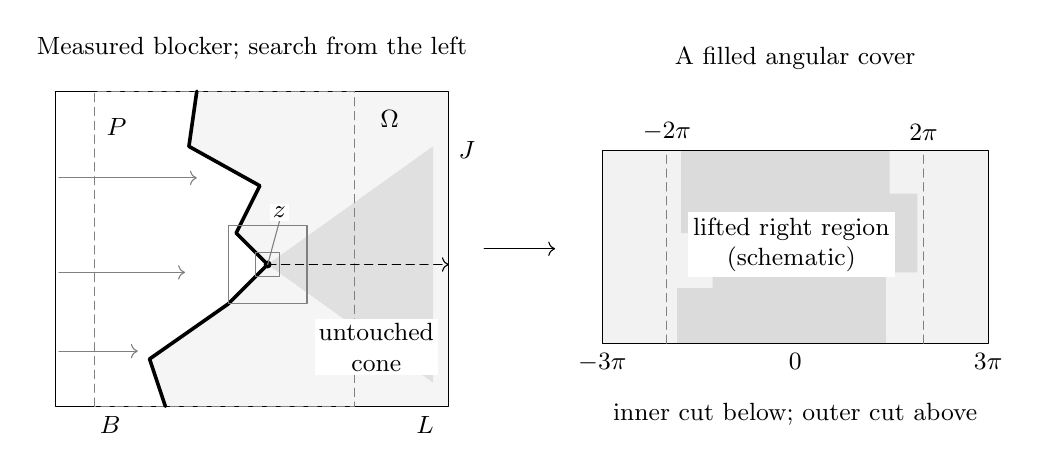
\begin{tikzpicture}[x=1cm,y=1cm,font=\small,line cap=round,line join=round]
  \path[fill=gray!8] (1.4,0) -- (1.2,.6) -- (2.2,1.3) -- (2.7,1.8) -- (2.3,2.2)
    -- (2.6,2.8) -- (1.7,3.3) -- (1.8,4) -- (5,4) -- (5,0) -- cycle;
  \path[fill=gray!24] (2.7,1.8) -- (4.8,.3) -- (4.8,3.3) -- cycle;
  \draw (0,0) rectangle (5,4);
  \draw[gray,densely dashed] (.5,0) rectangle (3.8,4);
  \draw[line width=1.3pt] (1.4,0) -- (1.2,.6) -- (2.2,1.3) -- (2.7,1.8) -- (2.3,2.2)
    -- (2.6,2.8) -- (1.7,3.3) -- (1.8,4);
  \draw[->,gray] (.05,.7) -- (1.05,.7);
  \draw[->,gray] (.05,1.7) -- (1.65,1.7);
  \draw[->,gray] (.05,2.9) -- (1.8,2.9);
  \draw[densely dashed,->] (2.7,1.8) -- (5,1.8);
  \draw[gray] (2.2,1.3) rectangle (3.2,2.3);
  \draw[gray] (2.55,1.65) rectangle (2.85,1.95);
  \fill (2.7,1.8) circle (.05);
  \draw[gray] (2.85,2.35) -- (2.7,1.8);
  \node[above,fill=white,inner sep=1pt] at (2.85,2.35) {$z$};
  \node at (.78,3.55) {$P$};
  \node at (4.25,3.65) {$\Omega$};
  \node[below] at (.7,0) {$B$};
  \node[below] at (4.7,0) {$L$};
  \node[right] at (5,3.25) {$J$};
  \node[fill=white,inner sep=1.5pt,align=center] at (4.08,.75) {untouched\\cone};
  \node[align=center] at (2.5,4.55) {Measured blocker; search from the left};
  \draw[->] (5.45,2) -- (6.35,2);
  \path[fill=gray!10] (6.95,.8) rectangle (11.85,3.25);
  \path[fill=gray!28] (7.9,.8) -- (7.9,1.5) -- (8.35,1.5) -- (8.35,2.2) -- (7.95,2.2)
    -- (7.95,3.25) -- (10.6,3.25) -- (10.6,2.7) -- (10.95,2.7) -- (10.95,1.7)
    -- (10.55,1.7) -- (10.55,.8) -- cycle;
  \draw (6.95,.8) rectangle (11.85,3.25);
  \draw[gray,densely dashed] (7.77,.8) -- (7.77,3.25);
  \draw[gray,densely dashed] (11.03,.8) -- (11.03,3.25);
  \node[below] at (6.95,.8) {$-3\pi$};
  \node[below] at (9.4,.8) {$0$};
  \node[below] at (11.85,.8) {$3\pi$};
  \node[above] at (7.77,3.25) {$-2\pi$};
  \node[above] at (11.03,3.25) {$2\pi$};
  \node[align=center,fill=white,inner sep=2pt] at (9.35,2.05) {lifted right region\\(schematic)};
  \node[above] at (9.4,4.15) {A filled angular cover};
  \node[align=center] at (9.4,-.1) {inner cut below; outer cut above};
\end{tikzpicture}
\caption{The path-defect geometry. The complete complementary-face search leaves the strict right side $\Omega$ of the measured path $P$ uninspected. An exposed vertex $z$ supplies the entire horizontal ray segment from $z$ to the right edge of $L$, with a cone portion contained in that side. After discarding supports hitting the $P$ hub, the annular part lifts to bounded angular coordinates. The pale rectangle on the right represents the larger regular sector used for coefficient transplantation, not an assertion that all of that sector was originally uninspected. External attachments leave through the outlet arc $J$.}
\label{fig:path-defect}
\end{figure}


\paragraph{Completing the collar and comparing coefficients.}
The ordered outlet $J$ permits a regular sector collar with separate
inner and outer attached graphs.  We now specify the source and target
of the coefficient comparison.  The
source is $G_\omega$, including all its original odds incident to
$p_\omega$.  Its allowed vertex set is
\[
 V_*=V(G_\omega)\setminus\{p_\omega\}.
\]
Construct a target graph $\widetilde G_\omega$ as follows.  Fill the
regular collar with angular range $[-3\pi,3\pi]$.  Each allowed source
vertex in the closed annular part of $\Omega$ is placed at its unique
lift.
The allowed vertices of $\Omega$ strictly inside the inner cut form
the inner attached graph.  All other allowed vertices form the outer
attached graph; this includes the left part of $L$, redrawn through its
outlets on $J$ as just described.  Cut vertices are the already placed collar
vertices, not new copies.  Each allowed source vertex is used once.
Identify $V_*$ with this set of target vertices and retain every
source edge between them, with its original odds.  All remaining
collar vertices are new filler sites.  The preceding outlet-order
argument shows that the two attached graphs induce permitted separate
caps and have no bypass around the collar.

It remains to check the incidence factors at the common allowed
sites.  At an allowed vertex strictly in $\Omega$, a required ordinary
neighbor missing from its lift can only be a vertex of $P$.  The
source edge to that vertex was uninspected with odds $v$, because
its interior lies strictly to the right of the blocker.  A new edge
to filler is charged to that old incidence.  There is at most one
charge in each original grid direction; if several source incidences
became parallel at $p_\omega$, their product still contains each
factor.  Thus the incident external product does not increase.

No new edge is added between two allowed vertices.  A required grid
edge between neighboring allowed vertices in consistent lifts was
already present in the untested source grid: a grid edge cannot cross
$P$ in its interior.  At either radial cut retain the old edges to
the corresponding attached graph and omit unneeded external edges.
The closed cut needs no filler continuation beyond it, so no
side-graph incidence is duplicated.  At allowed sites outside the
collar no new incidence is needed.  Remaining source edges to
$p_\omega$ may be discarded in the target.  Consequently the induced
graphs on $V_*$ agree and every target external product is at most
its source value.  Lemma~\ref{lem:transplant} applies with
$G_1=G_\omega$ and $G_2=\widetilde G_\omega$.

A connected support avoiding the hub, meeting the right inner ball,
and reaching a remote mark must cross both lifted cuts; it can exit
the right disk only through the far outlet $J$.  Its coefficient mass
in $G_\omega$ is dominated by the corresponding cut mass in
$\widetilde G_\omega$, since each of its allowed-site coefficients
can only increase.  Lemmas
\ref{lem:sector:cap-pressure} and \ref{sector:attached-sides} bound
that mass.  This contradicts density near $z$ after normalization by
the diverging mass.  For meshes bounded below, every counted support
hits one of the bounded number of vertices in the prescribed compact
hit set.  Equation~\eqref{sector:one-vertex-mass} gives the uniform
bound, exactly as in Lemma~\ref{sector:free-wall}.
The proof is unchanged under a grid rotation or primal-dual
interchange.
\end{proof}

\subsection{Annealing inside an annulus}
\label{sector:annular-annealing}

\begin{proposition}[Bounded annular cap densities]
\label{prop:annular-density}
Fix an ordinary square annulus of nonzero macroscopic width, with
inner and outer rim sets $A,E$.  There are $C<\infty$ and a mesh
threshold depending only on $q$ and this fixed geometry such that,
below that threshold, every pair of separate noncrossing cap
partitions $X,Y$ on the two rims satisfies
\begin{equation}
 |I_H(X,Y)|\le C.
 \label{sector:annular-I}
\end{equation}
The four pressures in $H,H/X,H/Y,H/(X,Y)$ between the rim images
are uniformly bounded as well.

The same conclusions hold for a fixed ordinary rectilinear polygonal
annulus between two disjoint simple boundary cuts with positive
separation.  Constants may depend on this geometry; each rim must
have a positive-length flat patch, and the ordinary bulk between
the cuts must be connected.  In particular a fixed thin ordinary
polygonal collar with these properties is allowed.

After attaching arbitrary planar graphs separately beyond the two
cuts, changing an allowed cap on one side changes the opposite-side
edge marginal by a uniformly bounded density and reciprocal density.
This is a bounded comparison, not a density tending to one.
\end{proposition}

\begin{proof}
Put $X_0=Y_0=\varnothing$, $X_1=X$, $Y_1=Y$, and use the notation
$Z_{ij}$ from Lemma~\ref{sector:mixed-identities}.  We must bound above
and below the ratio
\[
 T=\frac{Z_{11}Z_{00}}{Z_{10}Z_{01}}=\exp(-I_H(X,Y)).
\]
A free rim will bound the three pressures with at least one blank cap,
and hence bound $T$ above.  For the lower bound we expose a local primal
or dual path, use its conditional pressure bound, and sum over the
successful search leaves.

\paragraph{One blank rim and patch marginals.}
The pressures $\Delta_{00},\Delta_{10},\Delta_{01}$ are bounded.
For example, in $H/X$ the opposite rim $E$ is a pristine free wall.
Take $V$ to be the open annular bulk and choose a compact strip
separating its two rims.  Every connected support meeting both rim
sets meets that strip.  On a flat patch of $E$, choose the fixed
half-box $W$ and smaller $W_0$ of Lemma~\ref{sector:free-wall};
they fit inside the annulus away from its corners, with no attachment
across $E$.  The other rim $A$ stays a fixed positive distance from
$\overline{W_0}$.  The lemma therefore applies with the same data
for every $X$.  The cases $01$ and $00$ follow with the roles
interchanged.

Choose a small rectangle $B$ strictly inside the annulus and its
horizontal enlargement $L$, also strictly inside, so that the
remaining bulk around $B$ is connected.  Enlarge the initial patch
slightly if necessary to contain all edges of the primal and dual
searches used below.  Its edge marginal under either $10$ or $01$ is
uniformly comparable, in both directions, with that under $00$.
To prove this assertion, first remove the inside edge set and fix
one of its states.  Its components induce a noncrossing cap $U$ on
the new hole rim.  On the remaining graph consider the interaction
of $X$ with $U$, keeping $E$ blank.  Each of the four terms in
\eqref{sector:four-Delta} now tests $A$ against the hole rim.  Choose
a fixed compact strip separating $A$ from that hole in the connected
bulk outside it.  The same flat free-wall half-box at $E$ remains
available and both tested sets stay away from its smaller half-box.
Thus all four terms
are bounded by Lemma~\ref{sector:free-wall}; consequently
$|I(X,U)|$ is uniformly bounded over the inside states.  The same
argument compares $Y$ and $U$ with $A$ blank.  Inside edge weights
and component factors not touching the hole are independent of the
remote cap.  Component counting and normalization therefore give
constants $c_1,C_1>0$ such that for every patch event $F$,
\begin{equation}
 c_1\PP_{00}(F)\le\PP_{10}(F),\PP_{01}(F)
 \le C_1\PP_{00}(F).
 \label{sector:patch-marginals}
\end{equation}
Edges on the patch boundary can be assigned to its inside set; this
only changes the hole cut by bounded mesh steps.

\paragraph{A successful primal or dual leaf.}
In the blank law $00$, either a primal vertical crossing of a smaller
fixed rectangle has probability at least $1/2$, or its complementary
dual horizontal traversal does.  This is the finite disk path/cut
alternative, independent of the exterior edge states.  In the dual
case trim the first and last portions to obtain a crossing between
the first and last columns of an ordinary rectangle of dual cell
centers.  Its probability retains the same lower bound, and its
macroscopic dimensions stay nondegenerate.  Select the color and
orientation by this deterministic comparison of probabilities.
Perform the extremal complementary-face search from a perpendicular
side in that color.  Its success probability under $00$ is bounded
below by a fixed positive number.  Let $\omega$ denote a measured
leaf of the search, and let $Z_{ij}[\omega]$ be the partition sum
restricted to its prescribed measured states.

For every successful leaf,
\begin{equation}
 \left|\log\frac{Z_{10}[\omega]Z_{01}[\omega]}
                         {Z_{00}[\omega]Z_{11}[\omega]}\right|
 \le C_2.
 \label{sector:successful-leaf-ratio}
\end{equation}
For a primal success, delete the measured-closed edges and contract
the measured-open edges.  The fixed edge-odds factors cancel from
the ratio.  The resulting untested graphs have the same clear bulk
outside the search rectangle and the same measured blocker.  To check
the fixed data in Lemma~\ref{lem:sector:path-defect}, take
$V_{\rm bulk}$ to be the open annular bulk and $V_0$ to be its connected
complement of $B$.  The middle of the enlarged right edge has a fixed
open neighborhood in $V_0$.  Choose $C_*$ to be a compact strip near
the inner rim, separating the two rims and disjoint from $B$.
In each of the four cap quotients, a support joining the rims meets
$C_*$: the caps act separately on the rims and give no bypass across
this ordinary strip.  These choices are independent of the leaf and
caps.  Lemma
\ref{lem:sector:path-defect} bounds all four conditional pressures.
Equation~\eqref{sector:four-Delta} gives
\eqref{sector:successful-leaf-ratio}.

For a dual success, apply plane random-cluster duality before
conditioning.  Draw each primal cap as a noncrossing forest inside
its own complementary rim face and contract it.  The dual can be
represented on one common graph of cell centers and boundary slots:
each exposed rim edge carries its ordinary dual spoke to a slot,
and the slots are identified according to the complementary face
pieces left by that cap forest.  The two rim choices act separately.
These are noncrossing slot partitions, though their bases need not
be empty.

For completeness, the scalar factors in this duality do not affect
the mixed ratio.  The physical primal graph is connected, and
contracting the cap forests lowers its vertex number by the sum of
their two contraction ranks.  Euler's duality formula on the same
physical edge set, retaining loops, therefore has a fixed factor
times one factor for the inner cap and one for the outer cap.  All
three factors cancel from the four-term mixed ratio.  The same is
true after restricting to complementary measured states.  The
dual bulk grid has odds $q/v=v$.  Its successful path gives the
same conditional defect: after a fixed small shrinkage of the bulk
buffers, the preceding $V_{\rm bulk},V_0,N_+,C_*$ choices also work
for the shifted dual grid and its rim slots.  Arbitrary base slot caps
are allowed in
\eqref{sector:four-Delta}.  This proves
\eqref{sector:successful-leaf-ratio} for a dual success as well.

\paragraph{Summing the leaves.}
Write
\[
 T_\omega=\frac{Z_{11}[\omega]Z_{00}[\omega]}
                  {Z_{10}[\omega]Z_{01}[\omega]},\qquad
 p_{ij}(\omega)=\frac{Z_{ij}[\omega]}{Z_{ij}}.
\]
All prescribed finite edge states have positive weight.  Direct
multiplication gives
\[
 T_\omega\frac{p_{10}(\omega)p_{01}(\omega)}{p_{00}(\omega)}
 =\frac{Z_{11}[\omega]Z_{00}}{Z_{10}Z_{01}}.
\]
Summing this identity over all leaves equals $T$.  Restricting the
sum to successful leaves, using
\eqref{sector:successful-leaf-ratio} and
\eqref{sector:patch-marginals}, yields
\begin{align}
 T&\ge\sum_{\omega\text{ successful}}
       T_\omega\frac{p_{10}(\omega)p_{01}(\omega)}{p_{00}(\omega)}
       \notag\\
  &\ge e^{-C_2}c_1^2
       \sum_{\omega\text{ successful}}p_{00}(\omega)
   \ge c_2>0.
 \label{sector:annealed-lower-bound}
\end{align}
No comparison with the $11$ marginal has been used.
Conversely \eqref{sector:four-Delta} gives
\[
 \log T=-\Delta_{00}+\Delta_{10}+\Delta_{01}-\Delta_{11}
 \le\Delta_{10}+\Delta_{01}\le C_3,
\]
because all pressures are nonnegative.  The two bounds on $T$ prove
\eqref{sector:annular-I}.  Solving the same identity for
$\Delta_{11}$, and using the already bounded three other terms,
bounds the double-cap pressure.

\paragraph{Geometry and attached marginals.}
The proof used only connected clear bulk between separated cuts, a
flat free-wall patch at either blank rim, and a small interior search
rectangle whose complement is connected.  Every fixed rectilinear
polygonal annulus in the statement has these properties.  Choose all
patches and buffers at fixed positive distance from its finitely many
corners; bounded mesh roundings preserve the choices.  The preceding
proof therefore applies with constants depending on that geometry.
For a fixed thin collar the constants may be large, but remain
finite and mesh-independent.  Finally apply
Lemma~\ref{sector:attached-sides}, or condition on separate side
states and normalize their uniformly bounded partition-gain ratios,
to obtain the asserted marginal density comparison.
\end{proof}

\section{Irregular disks and physical connections}\label{sec:disks}

This section obtains uniform bounds for actual paths in irregular tiled
disks.  Its first input is the pressure contact construction: two walls
approached through clear ordinary bulk have a positive network connection
probability.  We prove the geometric localization needed to apply this
input in disks with slits, pinches, and separate boundary incidences.
Pure network decay follows by duality and the paired-list argument.
A second geometric construction then lets us extend actual central
crossings to two end wires, yielding actual hard-passage decay with
arbitrary planar joint end caps.

Actual decay leads to confined physical joins through a branching
estimate and a comparison of central marginals.  These joins build
routing and screens, which in turn give relative collar comparison
and splices that preserve an existing rare arm while blocking an
opposite-color arm.  All laws in this section are finite positive FK
laws at the fixed parameter $0<q<1$.  Ordinary tile and collar bonds
have odds $v=\sqrt q$; attached-graph edges may have any positive odds.
Conditioning on a measured leaf has the meaning of
Lemma~\ref{lem:finite-conditioning}.

\subsection{Disk conventions and the two pure tests}

\begin{convention}[Tiled disks and cut cells]\label{disk:conventions}
The mesh is one until a rescaling is explicitly made.  Square
checkerboard tiles have alternating primal and dual corners; their
monochrome diagonals are complementary bonds, with ordinary odds
\(v=\sqrt q\).  A tiled disk has an interior embedded injectively in
the plane, disjoint tile interiors, and no boundary image in its
interior.  Distinct boundary incidences may have the same physical
position.  All slots, paths, and cyclic orders at a cut or slit refer
to the disk, not to the quotient obtained by identifying such positions.

A boundary may cut a tile along a diagonal.  In the retained half-tile
put a virtual slot of the other color at the midpoint of that diagonal.
The half-tile is a four-slot cell with the two usual complementary bond
choices, one being a spoke to the virtual slot.  Its single random
bond has the ordinary odds.  The diagonal side can be bent infinitesimally
into the disk when defining topology.  A free untested virtual slot
contributes only a dangling edge.  Every interior tile is complete,
slot fans are internal to the disk, and successive boundary slots
alternate in color.

An \emph{actual} path uses physical open bonds and does not hop along
boundary identifications.  A \emph{network} test uses the specified
identifications in its component count and tests connection of its
terminals.  In particular, with just two separately wired end intervals,
network connection is equivalent to an actual path between some of
their slots, although its law is not the blank law.
\end{convention}

Let \(Q\) be such a quadrilateral disk, with disjoint end intervals
\(I,J\), each containing a slot of the tested color, and longitudinal
flanks \(S,T\).  Suppose that \(I\) lies in \(B(z,r)\) and
\(J\) lies outside \(B(z,R)\).  Either Euclidean or tile-coordinate
sup-norm balls may be used, changing only fixed constants.  Let \(p(Q)\)
be its tested-color connection probability with \(I,J\) separately
fully wired and with no other ties.  Write
\[
 u=1-q,\qquad t=q^{-1},\qquad
 H(a)=\frac{1-a}{1-u a},\qquad
 j(a)=-\log(1-u a).
\]
Here \(H\) is the same duality involution denoted by \(\mathcal H\)
in Section~\ref{sec:sectors}.

\begin{lemma}[The companion pure test]\label{disk:dual-test}
The separate-full-flank network probability in the opposite color is
\(H(p(Q))\).
\end{lemma}

\begin{proof}
Realize each end wire by a narrow chain along its boundary interval,
between successive tested slots.  The dual slots strictly inside these
chains have their own faces.  All remaining exterior dual slots belong
to one face: they are exactly the two longitudinal flank intervals,
joined for weighting.  Interior bonds are in diagonal or spoke
duality cell by cell.  The disk path/cut alternative identifies absence
of the tested end connection with an actual opposite-color connection
between the flanks, ignoring their common identification.

Let \(a\) be the connection probability when these two flank wires
are separate.  Joining them multiplies weights by \(t\) on separation
and by one on connection, so the actual connection probability becomes
\(a/(a+t(1-a))\).  Equating this with \(1-p(Q)\) gives
\(a=H(p(Q))\).  Specifying the first and last eligible slots moves the
four corner positions by only bounded mesh distance.
\end{proof}

\subsection{A network connection through an untouched channel}

We first isolate a pressure comparison at a small gap.  A \emph{hub}
means an existing terminal or a set of vertices already identified
there.  In particular, all vertices of a measured simple open path
belong to its hub.

For two vertices $x,y$ of a finite FK graph, the full-wire gain identity
gives
\[
 \Delta_G(\{x\},\{y\})
   =j\bigl(\PP_G(x\leftrightarrow y)\bigr).
\]
This includes hub vertices.  Thus a lower bound on the positive pressure
mass hitting both hubs is exactly a lower bound on their network
connection probability.

\begin{lemma}[Two-barrier pressure contact]\label{disk:pressure-contact}
Consider an annulus with a distinguished diameter and a focal half-ray
of that diameter.  Two barriers assigned to hubs \(x,y\) span the
annulus in opposite open half-planes, with many mesh steps of margin
from both diameter rays.  On the focal side, the component accessible
from the ray before meeting either barrier is ordinary uninspected
grid, with ordinary incidence up to its contacts.  All accessible
contacts in either angular direction have that direction's single
hub label.  These conditions hold on a slightly radially enlarged
annulus; barriers may fold or have several branches.

For a sufficiently large fixed ratio of outer to inner radius, the
network probability \(x\leftrightarrow y\) is bounded below by a
positive constant.  The bound is uniform in the exterior graph and
in its measured states and ties.  The conclusion does not require
the connecting network path to remain inside the channel.
\end{lemma}

\begin{proof}
Work first in the complete tested monochrome grid on an angular lift.
Choose a regular sector \(D\) whose angular walls lie at least \(2\pi\)
in either direction from the focal ray.  Its radial band is deep:
two comparable-radius patches, one on each angular wall, are separated
from either radial end by a large multiplicative factor.  Wire the
patches separately and call the resulting terminals \(x',y'\).
The fixed sector flank-chord construction, extended cofacially from
a fixed-ratio subband, gives
\(\PP_D(x'\leftrightarrow y')\ge c_0>0\).  Consequently the pressure
mass hitting both terminals equals
\(j(\PP_D(x'\leftrightarrow y'))\ge j(c_0)\).

This paired mass can be kept away from both radial end rows \(E\).
By the rooted hitting identity, the mass hitting \(x'\) and \(E\)
is at most
\[
 \frac{u}{q}\,
 \PP_D(x'\leftrightarrow E\text{ fully wired}).
\]
Enlarge \(x'\) by all vertices in a central subband containing \(y'\).
By adjacent-terminal comparison, this enlargement does not decrease
the last probability.
An outward connection must now cross one of two ordinary regular
sector collars.  They are networks in parallel.  Conditional ties
from the other piece either keep their two terminals separate or
join them; joining upweights absence of an actual connection.
Their pure radial probabilities therefore give a union upper bound.
Proposition~\ref{prop:sector-network} makes this bound arbitrarily
small by choosing the radial depths large.  Fix the depths so that
at least \(j(c_0)/2\) of the paired pressure mass avoids \(E\).

We next place a copy of this sector chart across the actual channel.
Take as active its ordinary strict sites accessible from the focal
ray, before a barrier is met, in a slightly larger radial band.
Use radius-spanning barrier subarcs, trimmed from a last exit to a
first reach.  Between their angular lifts, each physical strict
site occurs once.  The active component does not reach the artificial
angular walls.  Every nearest-neighbor chart step from an internal
active site either remains active or has an ordinary contact edge
to its indicated hub, possibly a half-tile spoke.  There is no
missing incidence across the focal ray.  Extra folds simply remove
parts inaccessible from that ray.

Prewire into its indicated hub the active endpoint of every contact
incidence at an obstructed chart step, including immediate ordinary
contact incidences.  Read these incidences from a band slightly
larger than the template, so that the same prescription applies at
its radial ends.  The two absorbed sets stay apart because the
focal strip has many-step width.

This enlargement has a bounded reversible cost.  Hold one hub as
the rooted vertex and remove the incident edges of the other hub
to form the base graph in Lemma~\ref{lem:rooted}.  For each remaining
site $i$, put $s_i=\prod_{h\ni i,\,h\ni o}(1+v_h)$, the product over all
links from $i$ to the removed hub $o$; parallel links are included
separately.  Its connection probability is
\[
 \EE_\mu\left[1-\prod_i s_i^{-m_i}\right].
\]
Whenever a multiset meets the set being prewired, at least one
affected link has odds at least $v$, and the displayed integrand
is at least \(v/(1+v)\) times its full-wire limit.  Off that set
the integrands agree.  Thus an entire hub enlargement costs at most
\((1+v)/v\), independently of the number of absorbed sites.
Apply this once for each hub.

Fill the nonactive chart sites and identify each filler site with
the hub on its angular side of the focal strip.  Sites on further
sheets beyond the corresponding barrier have the same label.
No required chart edge connects two different such labels: the
untouched strip separates them throughout the enlarged radial
band.  Edges between retained strict sites, and edges from them
to a prewired neighbor, are present at their ordinary odds.
Every remaining required edge is a hub loop or an available
contact incidence.  In particular, if both sides of a missing
chart step are retained across two cut half-tiles, precollaring
has put both endpoints in the same hub.  The missing edge is
then a loop.  Add or allocate loop copies as necessary; this
does not change the enlarged network test.

Now split each hub into the distinct chart copies assigned to it,
the appropriate wired artificial patch \(x'\) or \(y'\), and
residual vertices carrying all other original edges.  The complete
chart \(D\) is present after splitting.  Merging the pieces back
does not decrease the terminal connection probability.  At all internal
chart sites the induced graph agrees with the benchmark, and
the incident products are no larger; extra original hub edges
have been assigned to residual pieces.  Only radial end rows
can retain unallocated outside incidences.  By
Lemma~\ref{lem:transplant}, coefficients supported on chart
multisets avoiding those rows are at least the benchmark
coefficients.  Positive coverage therefore gives paired pressure
mass at least \(j(c_0)/2\), hence a positive network connection
probability.  Reversing the two precollaring enlargements proves
the assertion in the original graph.
\end{proof}

\begin{lemma}[Auxiliary cleared-route construction]
\label{disk:auxiliary-contact}
In a bounded rescaled region, let two hub walls admit interior
tangent disks of radii bounded below, touching at \(z_1,z_2\).
Suppose their centers can be joined through ordinary uninspected
bulk by a path of bounded extent with fixed positive clearance
from all boundaries and nonordinary sites.  Near either contact,
all wall portions accessible from its tangent approach have the
same corresponding hub label, have ordinary incident edges up
to their slots, and extend out of a fixed small neighborhood.
Assume planar induced caps in buffered bulk boxes along the route.
Then, as the mesh tends to zero, the two-hub network probability
has a uniform positive lower bound.

The two local approaches may meet the same physical boundary
position, provided they are distinct accesses in disk topology.
The resulting connection is not asserted to remain in the route.
\end{lemma}

\begin{proof}
\emph{Buffered square events.}
In an ordinary clear box, horizontal actual crossings of a square,
or a rectangle whose transverse dimension differs by a bounded
number of steps, have probability bounded below uniformly in
planar exterior data.  Indeed a square crossing or its opposite
cell crossing has probability at least \(1/2\).  In the latter
case duality, a rigid grid symmetry, and bulk annular density
transfer that event to the desired color and direction in a
larger clear buffer.  The complementary cell crossing has
exterior adjacent rows; trimming changes dimensions only by
bounded steps.  One may instead start with a self-dual box
one step wider than its transverse height.

The same bounded-density transfer applies to a crossing with
endpoint constraints on any fixed convex clipped-square support.
Surround the whole support, within its positive clearance, by
two simple ordinary rectilinear polygonal cuts.  Their geometry
is fixed and nondegenerate, although the relative collar width
may be small.  The proof of
Proposition~\ref{prop:annular-density} uses connected clear
regions, straight-wall pieces with blank ends, and bounded
local path defects.  Each of these constructions fits along
these finitely many offset straight pieces, with constants
depending on their widths and angles.  Its pressure bounds
therefore give the same reciprocal density comparison here.
Rigidly moved copies may be compared through overlapping
larger neighborhoods.  Conditioning outside their buffers
only changes the allowed planar caps.  No physical hard
crossing or sector screen is used for this transfer.

\emph{A route and its templates.}
Choose a simple polygonal path with axis-parallel segments in
the tested monochrome grid directions, entering the tangent
disks along axis rays making angle at most \(\pi/4\) with their
inward normals.  It can be chosen with a bounded number of
segments, positive lower bounds on their lengths, and positive
clearance off its endpoint approaches.  To see uniformity,
join the two disk centers within their cleared corridor,
approximate by a sufficiently fine fixed pixel path, erase
loops, and perturb its axis segments inside the clearance.
Insert a small interior detour if necessary so both axial
directions occur.  A subsequential limit of cleared corridors
and contact normals gives the same conclusion with strict
sub-clearances.  If the physical endpoints coincide, fix
short rays in their separate accessible regions first, and
join their interior endpoints; simplicity is in the disk
topology.

Along this path place crossing templates, separated by small
positive gaps between their support envelopes.  Crop each
crossing between two straight transverse caps.  A finite
cover of each cap and pigeonhole selection give tiny endpoint
patches supporting a positive-probability crossing event.
Their widths can be made arbitrarily small relative to the
gap; their center displacements are then recorded.  Slight
cap shifts avoid vertices.  If a cap crosses a bond, use
the corresponding half-edge with its actual bond state and
orient the witness toward the far cap, retaining its portion after
its last near-cap hit and before its first subsequent far-cap hit.  Bounded
mesh rounding affects only these endpoint neighborhoods.

Here are explicit templates sufficient for the construction.
\begin{enumerate}[label=(\roman*)]
\item A straight \(+x\) advance of any prescribed fixed length
is made from two identical small horizontal-square crossing
templates, with one reflected to reverse its \(y\)-displacement.
The transverse displacements of their patch centers cancel.
Choose their widths just below half the desired advance and
allocate equal small gaps at the ends.  Longer advances are
subdivided to remain inside the chosen clearance.
\item For a \(+x\)-to-\(+y\) turn, use the support
\[
 [0,s]^2\cap\{x+y\le1.35s\}
\]
from its left edge to the oblique cap.  Crop a horizontal
crossing ending in the upper half, selected using reflection
and transfer.  Its endpoint has \(x+y\ge1.5s\), whereas its
starting point has \(x+y\le s\), so it crosses the cap.
Reflect and reverse traversal across that cap for the turn's
second half, with a small normal spacing.  The second support
is ahead of the vertical entry and the first is below the
horizontal exit by a fixed fraction of \(s\).  Much thinner
incoming and outgoing straight templates consequently miss
the nonadjacent half.  Grid symmetries give the other turns.
\item For a contact with inward normal proportional to
\((1,\tau)\), \(0\le\tau\le1\), use
\[
 [0,s]^2\cap\{x+\tau y\ge0.65s\}
\]
from the oblique cap to its right edge.  It is obtained by
cropping a horizontal crossing starting in the lower half.
Place the starting patch center a distance \(\epsilon\)
inside the contact along the normal, with
\[
 s^2/c'\ll\epsilon\ll s,
\]
where \(c'\) is the tangent radius.  Tangent-disk exclusion
then puts the whole template inside the clear approach and
the wall in the opposite half-plane in a smaller contact
annulus.  Every exit advances a fixed fraction of \(s\)
both axially and into the tangent half-plane.  Much thinner
subsequent straight templates are therefore safe.  Reverse
the construction at the other endpoint.
\end{enumerate}

Choose bend and endpoint sizes first, sufficiently small
relative to all route clearances and segment lengths.
Their selected patch offsets and gap displacements are
then fixed.  Adjust total advances on two independent
axis segments by the resulting small amounts, and realize
the intervening lengths by the straight cancellation
construction.  Its widths are much smaller than adjacent
bend or endpoint sizes.  The final gaps are smaller still,
and patch tolerances smaller than the gaps.  Bounds on all
segment lengths and widths give a finite bound on the
number of pieces before these last choices.  Thus the
remaining advances can be fitted exactly, up to bounded
mesh errors, without moving nonadjacent envelopes into
one another.  Near coincident endpoint closures the
envelopes stay in the separate tangent approaches.

\emph{Conditioning and network concatenation.}
The disjoint clear buffers give a positive joint probability
of all template crossings by successive conditioning.
On their success, perform the complementary-face searches of
Lemma~\ref{sector:frontier} in the separate clipped envelopes, always
from the same longitudinal side of the oriented route.  Seed only
the exterior flank face: an adjacent interior face is reached only
after its intervening physical bond has been queried closed.
Fictitious outward spokes confined to the endpoint patches specify
search topology only; they add neither FK ties nor physical path edges.
The complementary face search exhausts on success.  Setting every unqueried edge closed still leaves
a crossing, so a simple actual open blocker is supported
on measured edges.  No reached complementary face lies
beyond it, and ordinary incidences into its unsearched
side remain untouched.

At a gap, prolong the two blocker endpoints along their
short terminal spokes and connect them inside the innermost
gap neighborhood, solely for separation topology.  Between
a few gap widths and a small fixed fraction of the template
length the blockers span the annulus in opposite half-planes.
The focal ray on the unsearched side is in the untouched
gap.  An accessible fold terminates on the same blocker
hub; it introduces no foreign boundary condition.  Other
terminal caps are outside the enlarged join annulus.
At an endpoint the continuous wall and its short tangent
access replace one of the blockers.  Only its single wall
label is locally accessible, and tangent-disk exclusion
gives the same half-plane separation.

Lemma~\ref{disk:pressure-contact} therefore bounds every
successive two-hub connection below in the \emph{same}
conditional FK graph.  Hubs already connected cause no
difficulty.  Shared-root positive correlation gives
\[
 \PP(i\leftrightarrow k)
 \ge
 \PP(i\leftrightarrow j)\PP(j\leftrightarrow k).
\]
Iterating along the finite chain gives a positive conditional
probability of connection of the original hubs.  Averaging
over successful leaves proves the lemma.  This argument
does not claim simultaneous physical bridges confined
to the individual gaps.
\end{proof}

\subsection{Localization between irregular walls}

The contact lemma needs a clear route with controlled access to its
walls.  We now obtain such a route from an arbitrary long quadrilateral
disk.  The argument uses the topology of the split disk throughout;
closeness of two boundary images does not identify their incidences.
A related use of a minimal annulus to separate opposite boundary arcs
in the in-domain graph distance appears in
\citet[Section~4, following Fact~4.1]{DuminilCopinManolescuTassion2021}.
The diameter argument below also supplies the accessible-wall and
terminal-clearance properties needed in the present split-disk setting.

\paragraph{Integer level cuts.}
An integer tile-coordinate level separating the two end intervals
contains a proper tile-edge crosscut between the longitudinal flanks.
Indeed its preimage in the disk consists of finitely many interior
intervals with disjoint interiors, together with possible full level
circles.  A full circle cannot separate the end arcs in the embedded
disk.  Splitting along the proper intervals gives a tree of regions;
the tree path between the regions incident to the two ends contains a
cut separating them.  Its endpoints are on different flanks because
the level misses both ends.  Coincident boundary endpoints are resolved
in their separate fans.  The cut follows tile edges, meets a diagonal
boundary side only at a corner, and contains a whole edge with
alternating eligible slots.  The closed cut meets every end-to-end
path, including a boundary path by interior approximation.  Selecting
cuts backwards from the last desired level orders them intrinsically;
the intervening pieces are disks of Convention~\ref{disk:conventions}.

For the local argument regard a tiled disk as an abstract compact disk
$X$ mapped continuously into the plane.  Its interior maps injectively
onto an open set $D$, and no boundary image lies in $D$.  Write its
four arcs as $I,S,J,T$ in cyclic order.  An \emph{access} to a boundary
incidence is an interior arc ending there.  A \emph{proper} $S$--$T$
crosscut is a simple arc in $X$ with interior in $X^\circ$ and its
endpoints in the specified flank incidences.  Its diameter and every
distance below refer to physical images.  Write $N_s(K)$ for the
open physical $s$-neighborhood of a set $K$.

\begin{lemma}[Local labels and wall continuation]
\label{disk:local-access}
Suppose a closed physical ball $\overline B(z,s)$ misses the end arcs
$I,J$ and contains no proper $S$--$T$ crosscut of diameter at most $2s$.
For every component $U$ of $D\cap B(z,s)$, all original-wall incidences
accessible from $U$ have the same flank label.  For generic $s$, each
such wall occurrence has wall-only continuations in both directions
on the boundary of $U$ until that boundary first meets the circle.
These continuations refer to the approached side of a wall, including
at slit tips and split boundary fans.
\end{lemma}

\begin{proof}
Two accesses in a connected open component can be joined by an
interior polygonal path and then simplified to a proper arc, retaining
the endpoint incidences.  Opposite labels in $U$ would therefore give
the forbidden cut inside $\overline B(z,s)$.

The component $U$ is simply connected.  Indeed the complements of $D$
and the ball in the sphere are connected and meet; every complementary
domain of their union is simply connected.  For a generic radius the
finite polygonal cell structure gives a finite prime-end boundary walk
of $U$, consisting of original-wall and circle pieces.  Slit banks and
repeated physical vertices remain separate occurrences in that walk.
There is an open circle piece: join an interior point of $U$ to a point
of $D$ outside the ball, which exists since the end arcs lie outside.
Following the boundary walk from any original-wall occurrence in either
direction to its first circle occurrence gives the asserted wall-only
continuation.  Each intervening wall occurrence is accessible from $U$
and hence has the same label.  The exceptional radii consist of the
finitely many vertex and tangency values.
\end{proof}

\begin{proposition}[Localization in an intermediate shell]
\label{hyp:disk-localization}
Let $Q_n$ be disks of Convention~\ref{disk:conventions}, with end arcs
$I_n,J_n$ and flanks $S_n,T_n$.  Write $\varrho_n$ for sup-norm radius
about a tile-coordinate center, and suppose
\[
 I_n\subset\{\varrho_n\le r_n\},\qquad
 J_n\subset\{\varrho_n\ge R_n\},\qquad
 1+r_n=o(m_n),\qquad m_n=o(R_n),
\]
where $m_n$ is an integer.  Put
$\mathcal S_n(m_n)=\{3m_n/4<\varrho_n<5m_n/4\}$.
After passage to a subsequence one of the following alternatives holds,
with constants $a>0$ and $A<\infty$ fixed on that subsequence.
\begin{enumerate}[label=\textup{(\roman*)}]
\item There is a proper $S_n$--$T_n$ tile-edge crosscut of at most $A$
edges in the safe shell $\mathcal S_n(m_n)$.  Its incident cells contain
a physical bond route of either prescribed color between eligible
flank slots, after moving each contact at most $A$ tile steps within
its own fan.  In this case put $\ell_n=1$.
\item There are scales $\ell_n\to\infty$, with $\ell_n\le A m_n$,
and interior tangent disks of radii in $[a\ell_n,A\ell_n]$ touching
the respective flanks.  Their centers are joined by a simple polygonal
route of length at most $A\ell_n$, with an ordinary buffer of width
at least $a\ell_n$ away from its terminal approaches.  At either
contact, every wall portion accessible from the approach in a fixed
contact neighborhood has that flank's label and ordinary incident
bonds up to its slots, and continues physically out of a larger
contact neighborhood.  The neighborhood radii and all buffer widths
are fixed positive multiples of $\ell_n$; all named geometry lies in
$\mathcal S_n(m_n)$.

More precisely, with $\eta=10^{-3}$ there is a proper crosscut $K_n$
of diameter $\ell_n$ such that no proper $S_n$--$T_n$ crosscut of
diameter less than $\eta\ell_n$ meets $N_{\eta\ell_n}(K_n)$.
The tangent disks can have radius $\rho_n=\eta\ell_n/100$, with
centers on $K_n$, and their contact neighborhoods are contained in
this excluded neighborhood.  This geometry satisfies the hypotheses
of Lemma~\ref{disk:auxiliary-contact} in the companion pure law,
including the planar caps on clear bulk buffers.
\end{enumerate}
Both statements hold in the split disk, also when the two accesses
end at the same physical position through different incidences.
\end{proposition}

\begin{proof}
Suppress the sequence index.  We first choose a scale at which a
crossing between the two flanks
cannot be replaced by a much smaller nearby crossing.  This gives the
single-label terminal neighborhoods.

\paragraph{Diameter descent and the clear core.}
Choose a proper level cut $K_0$ at radius $m$, and write $L_0$ for its
physical diameter.  Thus $L_0\le3m$, after a fixed change between the
Euclidean and tile-coordinate norms.  Fix $\eta=10^{-3}$.  Starting
from a proper crosscut $K$ of diameter $L>1$, replace it whenever there
is a proper $S$--$T$ crosscut of diameter less than $\eta L$ meeting
the physical $\eta L$-neighborhood of $K$.  The replacement lies within
$2\eta L$ of $K$.  The diameters decrease geometrically, so after
finitely many replacements either $L\le1$ or no such replacement is
possible.  The total displacement from $K_0$ is at most
\[
 \frac{2\eta L_0}{1-\eta}<\frac m{100}.
\]
Pass to a subsequence on which the final diameters are bounded or tend
to infinity.  All subsequent constructions stay within a sufficiently
small fixed multiple of $L$ of $K$.  They therefore lie in the safe
shell and miss the end intervals.  Here and in this proof constants
may depend on the subsequence, but not on its index.

Consider the divergent case, and put $\ell=L$ and
$\rho=\eta L/100$.  An interior point $x$ of $K$ at distance at most
$\rho$ from the physical boundary has a nearest boundary point.  The
open segment to that point lies in the disk and determines an access
to a boundary incidence.  That incidence has a unique flank label:
two opposite-label nearest accesses would join through $x$ to give
a proper crosscut of diameter at most $2\rho<\eta L$.  More generally,
two sufficiently close parameters of $K$ in this boundary layer cannot
have different labels.  Their nearest-access segments and the short
intervening subarc would simplify to a proper cut of diameter at most
$4\rho$, again forbidden.  The label sets are consequently disjoint
closed subsets of the parameter interval.  Near the two endpoints they
have labels $S$ and $T$, respectively; the same short-access argument
proves this even at repeated physical boundary positions.

Take the first $T$-labeled parameter and the last $S$-labeled parameter
preceding it.  Both have boundary distance exactly $\rho$, and the
intervening core has boundary distance at least $\rho$.  Its endpoints
are centers of interior tangent balls of radius $\rho$ at the two
flanks.  Replace this core by a simple polygonal route inside its clear
neighborhood.  For a uniform construction, cover its diameter-$L$
bounding box by squares of side $\rho/100$, retain the squares meeting
the core, connect through them, and erase loops.  There are at most
$O((L/\rho)^2)$ squares.  Perturbing inside the $\rho/2$-clear region
gives a route of length $O(L)$ with clearance at least $\rho/4$.
A finer fixed grid and a short interior detour give axis segments of
controlled positive length, separated tubes around nonadjacent pieces,
and a protected straight central segment.  There are finitely many
combinatorial choices at this normalized scale.  A further subsequence
fixes a pattern and strict sub-clearances, including the inward approach
directions at the tangent balls.

At a tangent contact $z$ choose two small ball radii in fixed separated
subintervals of $(\rho/20,\rho/10)$.  For either such radius $b$,
\begin{equation}\label{disk:terminal-containment}
 B(z,b)\subset N_{\rho+b}(K)\subset N_{\eta L}(K),
 \qquad \rho+b<1.1\rho<\eta L.
\end{equation}
Every proper opposite-flank cut contained in this ball would have
diameter less than $\eta L$ and meet the excluded neighborhood.
Lemma~\ref{disk:local-access} therefore supplies the correct single
flank label and the wall continuations in the component approached
from the tangent ball.  Choose radii avoiding tangencies and vertices.
For a sequence there are only countably many exceptional normalized
radii, so the same normalized choices can be used throughout.

These facts prove the clear-route and local-wall assertions of the divergent
alternative.  The full and half-cell conventions provide ordinary
incidences up to the accessible wall slots.  In the companion law draw
the two separate flank wires as disjoint chains in narrow boundary
collars of the abstract disk.  Any exposure outside a clear bulk buffer
then induces a noncrossing cap on it.  This verifies the planar-cap
hypothesis of Lemma~\ref{disk:auxiliary-contact} directly from the
finite graph.

\paragraph{Bounded cuts and discretization.}
If the final diameter is bounded, perturb $K$ off the vertices and
follow its chain of full or half-cells through interior full tile sides.
A diagonal side of a retained half-cell is an original boundary side,
so no interior transition crosses it.  Erase repeated cells in the
adjacency chain.  Only boundedly many cells occur, since their interiors
are disjoint in a bounded region.  Each cell offers an ordinary bond
joining its two slots of either prescribed color.  Successive cells
share that color's slot on their common full side in the same fan.
Concatenation gives a bounded physical route between eligible flank
slots, with bounded endpoint moves within their original fans.

To obtain a proper tile-edge separator as well, replace each cell
passage by at most four full sides.  The full-side skeleton of a square
is connected, and the two nondiagonal sides of a retained triangle
connect all its three original corners.  Use the same corner of each
shared side for the two neighboring passages.  An endpoint on a
boundary diagonal moves to one of its corners in its own incidence.
This constructs a bounded tile-edge walk from $S$ to $T$.  All its
boundary visits lie in the safe shell, hence have label $S$ or $T$.
Stop at its first $T$ visit and start at its last preceding $S$ visit.
There is now no boundary incidence in its interior; in particular it
cannot contain an original boundary edge, whose incidences have a
single label.  Erase loops in the abstract graph.  The resulting
proper crosscut contains at least one full tile edge.  Finally perturb
this selected cut slightly into one side, within its incident cells
and endpoint fans, and repeat the color-route construction there.
Thus the bounded route lies in cells meeting the selected cut itself.
This proves the bounded alternative of the proposition.

\end{proof}

\subsection{Pure tests in irregular disks}

\begin{theorem}[Pure irregular-disk decay]\label{thm:pure-disk}
Uniformly over either color and all disks in
Convention~\ref{disk:conventions},
\[
 \lim_{L\to\infty}
 \sup_{\substack{I\subset B(z,r),\ J\cap B(z,R)=\varnothing\\
                  R/(1+r)\ge L}}
 p(Q)=0.
\]
\end{theorem}

\begin{proof}
Let \(M\) be the supremum limit in the assertion.  If \(M=1\),
choose disks \(Q_n\) of diverging end-separation ratio with
\(p(Q_n)\to1\), and then choose integer intermediate radii
\(1+r_n\ll m_n\ll R_n\).  Proposition~\ref{hyp:disk-localization} gives a subsequence and
constants fixed on it.
In the bounded alternative its opposite-color route uses boundedly
many tiles, with bounded moves to the eligible flank slots.  Conditional
finite energy gives a positive lower bound for the companion flank
connection.  In the divergent alternative,
Lemma~\ref{disk:auxiliary-contact} gives such a bound for the two
flank hubs of the companion pure law.  Either conclusion contradicts
Lemma~\ref{disk:dual-test}, since \(H(p(Q_n))\to0\).  Thus \(M<1\).
The lower bound here may depend on the extracted subsequence; no
uniform localization constants over all disks were needed.

Suppose \(M>0\), and take \(p(Q)\to M\) at diverging
end-separation ratios.  Put \(h=H(M)\in(0,1)\).
For any fixed list length, choose pairs of integer level
crosscuts
\[
 C_{s_i^-},\ C_{s_i^+}
\]
with all paired ratios, intervening gaps, and end
clearances diverging successively.  They can be ordered
intrinsically: select the last desired cut, retain its
piece containing \(I\), and repeat backwards.  The
intercut pieces are tiled disks of the same class,
with full cuts as ends.

For each isolated intercut disk, let \(a_i,b_i\) be precisely
the two companion flank electrodes prescribed by
Lemma~\ref{disk:dual-test}, including its eligible corner slots.
Embed these same slots in their accessible fans of the companion graph
of the full \(Q\), and wire each electrode separately there.
The cuts alternate slots and contain a whole edge.  Thus these are
exactly the isolated companion tests, with no independent endpoint
rounding; all electrodes lie on the original flanks away from the
original end corners.

Each matched probability has lower limit at least \(h\).
Indeed duality gives this for its isolated intercut disk,
and cofacial extension preserves the lower bound.
For this extension all unwanted graph is beyond the
tile cuts and can be peeled through those end openings
from the exterior faces of a terminal test edge.
The wire chains hug their exposed boundary subintervals
and seal no unwanted region.  A corner gaining extra
incidences upon extension is interpreted in its same
accessible disk fan.  The other disjoint interval
chains can then be added by the same exterior
cofacial argument.

Conversely merge all \(a_i\)'s, merge all \(b_i\)'s,
and complete both flank intervals.  Adjacent-terminal
comparison shows that the test does not decrease; the final test is the
companion probability of \(Q\), which tends to \(h\).  Therefore
every merged cross-list subgroup test containing a
matched pair tends to \(h\).

For two ordered-separated nonempty index sets \(U,V\) on the first
list, enlarge their terminals to the two complete cuts of an unused
intervening diverging-ratio gap.  No other local interval wire bridges
that gap.  Each exterior now attaches only at its own terminal and
factors out, leaving the pure radial test of an intercut disk of this
class.  In the notation \(G\) of \eqref{sector:merger-functional},
terminal enlargement in the original finite hub graph and then this
gap comparison give, for every \(i\in U,j\in V\),
\[
 \PP(a_i\sim a_j)\le G(a_U,a_V)\le M+o(1).
\]
Choose \(c_*=(1-M)/2>0\) before choosing the list length.  For each
fixed length the last upper bound is at most \(1-c_*\) sufficiently
far along the disk sequence, simultaneously for its finitely many
ordered-separated groups.

The induced partition has the reversed boundary orders of
Lemma~\ref{lem:sector:paired-lists}; pressure coverage gives its
inequalities \eqref{sector:partition-pressure}.  For each fixed list
length, take a subsequential limit in its finite partition simplex.
The matched and cross-list subgroup tests converge to \(h\), and the
same-list bounds above survive.  Let the list length increase and take
a projective subsequential limit, as in the proof of
Proposition~\ref{prop:sector-network}.  Every fixed finite constraint holds
eventually, and the merger denominators are positive.  The resulting
partition law satisfies all hypotheses of
Lemma~\ref{lem:sector:paired-lists} with \(c=c_*\), a contradiction.
Hence \(M=0\).
\end{proof}

\subsection{Separated cuts and a clear terminal probe}

Pure decay will control the cost of changing end weights.  To extend
the resulting central actual crossing, we also need an untouched route
from an end wire to a measured crossing.  The next geometric lemma
provides two possible entrances and a clear probe toward either flank.

\begin{lemma}[Two families of separated cuts]\label{disk:four-cuts}
Under the hypotheses of Proposition~\ref{hyp:disk-localization},
suppose also that $m_n=o(m'_n)$ and $m'_n=o(R_n)$ for integers $m'_n$.
On one subsequence choose localization data in both safe shells.
At a bounded-scale shell use its bounded-length cut as $C_0$.
At a divergent-scale shell, with scale $\ell_n$, one can choose four
proper tile-edge $S_n$--$T_n$ cuts $C_0,C_1,C_2,C_3$ such that each
has length at most $A\ell_n$ and
\[
 \dist(C_i,C_j)\ge a\ell_n\qquad(i\ne j).
\]
Constants may differ between the shells, but are fixed on the
subsequence.  The regions between consecutive cuts are admitted disks
with those cuts as ends and no additional longitudinal boundary.
The following geometry lies in the same safe shell.
\begin{enumerate}[label=\textup{(\roman*)}]
\item In a common ordinary interior rectangle, separated from the
original boundary by at least $a\ell_n$, the cuts are straight parallel
segments.  Two separated transverse strips, each of width at least
$a\ell_n$, run from flat $C_0$ patches through openings in $C_2$ to
$C_3$.  The openings are separated from each other and from the segment
ends by at least $a\ell_n$.  Fixed physical neighborhoods of these
openings miss every nonlocal portion of $C_2$.
\item From either strip, the portion of $C_3$ toward either flank has
an ordinary clear corridor of width at least $a\ell_n$ until entering
its terminal neighborhood.  It stays at distance at least $a\ell_n$
from $C_2$, the other shell's cuts, and unrelated original walls.
At each end the terminal neighborhood and its enlargement are the
accessible parts of physical balls centered at the actual cut endpoint,
of radii $b\ell_n,b^+\ell_n$, with
$a\le b$, $b+a\le b^+\le A$.  Their normalized radii are fixed on the
subsequence.  In the larger neighborhood only the indicated flank is
accessible from the corridor, and every accessible wall occurrence
continues physically out of that neighborhood.  The corridor and
neighborhood assertions use the separate incidences at coincident
physical boundary positions.
\end{enumerate}
The families do not interleave.  With primes for the second shell,
their intrinsic order, up to reversal, is
\[
 C_0,C_1,C_2,C_3,C'_3,C'_2,C'_1,C'_0,
\]
with $C_1,C_2,C_3$ omitted at a bounded end.  Each family has a clear
interior connector of length at most $A\ell_n$ crossing its cuts in
order.  The disk $F$ between $C_0,C'_0$ is admitted, and its end-separation
ratio tends to infinity.
\end{lemma}

\begin{proof}
We use the full-side skeleton rounding of
Proposition~\ref{hyp:disk-localization} at divergent scale.  A curve consisting
of boundedly many line or circle pieces of total length $O(\ell)$
meets $O(\ell)$ cells.  The same skeleton construction stays within
$O(1)$ tile steps and uses $O(\ell)$ edges.  Keep a grid-aligned central
segment and follow each outward branch to its first original-wall
incidence.  Macroscopic clearance places that incidence in the intended
terminal neighborhood, with its correct label.  Loop erasure preserves
the central segment and the separated branch tubes.  Opposite accesses
in coalescing terminal neighborhoods cannot meet in the interior,
since that would give an excluded small opposite-flank cut.

There is a useful refinement when the final approach is the radial
segment from the center $x$ of an interior tangent ball to its contact
$z$.  At every point $y$ on this segment,
\begin{equation}\label{disk:radial-clearance}
 \dist(y,\partial D)=|y-z|.
\end{equation}
The upper bound uses $z$ and the lower bound uses the tangent ball.
Hence an earlier contact caused by rounding is only $O(1)$ steps from
$z$.  If $\widetilde z$ is the rounded endpoint, center the terminal
balls at $\widetilde z$ and choose their normalized radii generically
in slightly smaller fixed intervals, still separated by a fixed gap.
The displacement $|\widetilde z-z|=O(1)=o(\ell)$ preserves strict
containment and separation.  Reapplying
Lemma~\ref{disk:local-access} in these recentered balls gives wall
continuations at the actual cut endpoint.  We use precisely these
endpoint-centered neighborhoods below.

\paragraph{Four cuts in one shell.}
We construct the four cuts first in one shell.  Rescale by
$\ell$ and suppress the sequence index.  The preceding clear route
enters each tangent disk along an axis ray strictly inside its inward
cone.  If the two contacts stay a positive distance apart, choose
disjoint terminal work balls smaller than this distance.  The case of
coalescing contacts will be checked separately.

Inside each single-label neighborhood fix
\[
 0<h_0<h_1<h_2<h_3,
 \qquad 0<d_0<d_1<d_2<d_3\ll h_0.
\]
The radii have positive gaps, for example successive ratio four, and
$h_3$ is much smaller than the tangent radius, the neighborhood radius,
and $\eta$.  The offsets also have positive gaps.  Draw four parallel
copies of the core, on the prescribed longitudinal side.  Near each
end truncate the $i$th approach ray at radius $h_i$ about the old
contact and follow that circle in the corresponding longitudinal
direction.  For $i=0,1,2$, stop at the first wall hit.  Such a hit exists:
the accessible wall continuation from the contact leaves the largest
work ball, and so crosses this circle.  The first hit has the intended
flank label.  The old tangent disk excludes walls from a fixed cone
about its inward ray, so the tail stops before returning through the
opposite margin of that cone.

The four curves are separated for explicit geometric reasons.  Tails
on distinct circles have their radial gap.  An outer approach ray
starts outside every smaller circle.  At its beginning an outer tail
moves farther to the chosen side of the smaller-offset rays, retaining
the offset gap; away from that cone its distance from an inward ray
is a fixed fraction of its radius.  It cannot return through the
other cone margin before its first wall hit.  The nonterminal pieces
retain their separate core tubes.  All these are strict bounds by
positive constants in the rescaled geometry.

The outermost curve requires a further change: a tail stopped at its
first exact wall hit need not have clear passage to that hit.  Choose
$\delta>0$ smaller than all radial and offset gaps, tube widths, and
terminal containment margins.  Follow the outermost ray and its
$h_3$ tail only to its first point $x$ at distance $\delta$ from an
original wall.  Its earlier part is $\delta$-clear.  Choose a nearest
contact $z$ and complete this end by the segment $xz$.  Then
$B(x,\delta)$ is an interior tangent ball, and $z$ has the correct
accessible label.  The new segment stays within $\delta$ of $x$,
so all separation margins survive.  Its interior has boundary distance
strictly less than $\delta$, by \eqref{disk:radial-clearance}; it
therefore cannot meet the retained, $\delta$-clear part of the curve.

Choose smaller and larger terminal radii near $\delta/8$ and
$\delta/4$, with a fixed gap and generic values.  Their balls about
$z$ are contained in the old single-label neighborhood and miss $C_2$.
The retained probe and its radial end segment connect the approached
components to the old tangent approach.  Lemma~\ref{disk:local-access}
again gives their label and wall continuations.  Equation
\eqref{disk:radial-clearance} supplies a corridor of width less than
one quarter of the smaller radius until that corridor enters the
smaller terminal ball.  This constructs the required clear terminal
probe for $C_3$; no clearance is needed on the discarded remainder of
the exact-hit tail.  Figure~\ref{fig:disk-localization} depicts this
choice and the protected central openings.

\begin{figure}[tbp]
\centering
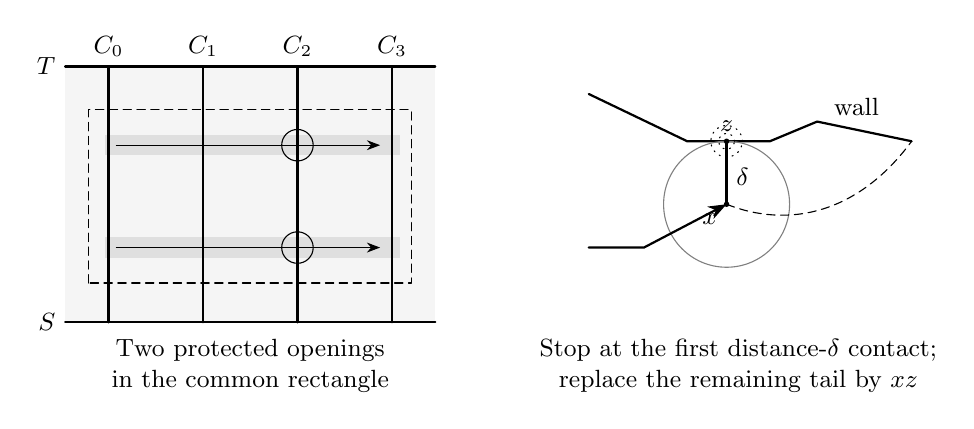
\begin{tikzpicture}[x=1cm,y=1cm,font=\small,line cap=round,line join=round]
 \begin{scope}
  \fill[gray!8] (-.35,.3) rectangle (4.35,3.55);
  \draw[thick] (-.35,.3)--(4.35,.3);
  \draw[thick] (-.35,3.55)--(4.35,3.55);
  \node[left] at (-.35,.3) {$S$};
  \node[left] at (-.35,3.55) {$T$};
  \fill[gray!25] (.15,1.12) rectangle (3.9,1.38);
  \fill[gray!25] (.15,2.42) rectangle (3.9,2.68);
  \draw[densely dashed] (-.05,.8) rectangle (4.05,3.0);
  \foreach \x/\i in {.2/0,1.4/1,2.6/2,3.8/3} {
   \draw[thick] (\x,.3)--(\x,3.55);
   \node[above] at (\x,3.55) {$C_{\i}$};
  }
  \draw[-{Stealth}] (.3,1.25)--(3.65,1.25);
  \draw[-{Stealth}] (.3,2.55)--(3.65,2.55);
  \draw (2.6,1.25) circle (.2);
  \draw (2.6,2.55) circle (.2);
  \node[align=center] at (2,-.25) {Two protected openings\\in the common rectangle};
 \end{scope}
 \begin{scope}[xshift=6.2cm]
  \draw[thick] (.1,3.2)--(1.35,2.6)--(2.4,2.6)
       --(3,2.85)--(4.2,2.6);
  \node[above] at (3.5,2.8) {wall};
  \draw[gray] (1.85,1.8) circle (.8);
  \draw[thick,-{Stealth}] (.1,1.25)--(.8,1.25)--(1.85,1.8);
  \draw[thick] (1.85,1.8)--(1.85,2.6);
  \draw[densely dashed] (1.85,1.8)..controls(2.6,1.5)and(3.5,1.65)..(4.2,2.6);
  \fill (1.85,1.8) circle (.035);
  \fill (1.85,2.6) circle (.035);
  \node[below left] at (1.85,1.8) {$x$};
  \node[above] at (1.85,2.6) {$z$};
  \node[right] at (1.85,2.15) {$\delta$};
  \draw[dotted] (1.85,2.6) circle (.2);
  \draw[dotted] (1.85,2.6) circle (.1);
  \node[align=center] at (2,-.25) {Stop at the first distance-$\delta$ contact;\\replace the remaining tail by $xz$};
 \end{scope}
\end{tikzpicture}
\caption{The geometry used to extend an actual crossing.  Left: the
common straight portions of four separated cuts contain two transverse
strips and protected $C_2$ openings.  Outside this rectangle the cuts
may follow irregular walls.  Right: a schematic terminal probe for
$C_3$.  Its retained part is $\delta$-clear, and the nearest-wall segment
from its first distance-$\delta$ point $x$ supplies a tangent approach
to $z$.  The dashed remainder of the old exact-hit tail is discarded;
the dotted circles indicate the smaller terminal neighborhoods.
Neither panel depicts the full disk or asserts separation of distinct
incidences having the same physical boundary position.}
\label{fig:disk-localization}
\end{figure}


\paragraph{Coalescing contacts.}
It remains to check physical separation when the two original tangent
contacts converge to the same position.  The small-cut exclusion implies
that their inward normals in the limit are opposite.  Otherwise the
two equal-radius tangent disks overlap in a sector arbitrarily close
to the common contact.  Joining their radial accesses through that
sector would give a forbidden proper $S$--$T$ cut.  Choose axis rays
strictly inside the resulting opposite inward cones, and use the same
list of radii at the two ends.

Distinct tail indices are separated by their radial gap, less the
vanishing contact displacement.  To control a tail against an
opposite-end ray, take a fixed strict subcone about that ray.  At
radii between $h_0$ and $2h_3$, balls of radius $c h_0$, for sufficiently
small fixed $c>0$, lie inside the opposite tangent disk and connect
to its contact by the radial access.  If the tail entered one of these
balls, its own contact access, the tail, and a short connection in the
ball would produce an excluded local $S$--$T$ cut.  Thus every tail
stays a positive distance from every opposite-end approach ray.  The
same bound holds for offset rays by choosing all $d_i$ below this
margin and reducing $c$.  Beyond radius $2h_3$, radial distance alone
separates a ray from every circular tail, whose radius is at most $h_3$; the
vanishing contact displacement and the smaller offsets preserve this
gap.  Tail-to-tail distances use the distinct
radii.  Decrease $\delta$ below these margins too, so the terminal
replacement within distance $\delta$ preserves them.  Each tail
remains in its own circle component.  The two
first-distance-$\delta$ approaches cannot meet through the local
clear bulk either, since such a meeting would join the two accesses.
Physical coincidence of the two endpoints of a single cut is allowed
in different boundary incidences; the four distinct cuts remain
physically separated.

Round the curves as described above.  Fixed positive separations
survive the $O(1)$ displacement, and the final terminal balls are
recentered at the actual rounded endpoints.  In a smaller protected
central rectangle the four cuts are straight parallel segments.
Choose two separated transverse strips through this rectangle from
flat $C_0$ patches across $C_2$ to $C_3$.  Reserve a fixed physical
neighborhood of each $C_2$ opening disjoint from all nonlocal portions
of $C_2$: the separated core tubes and the smaller rectangle give
this stronger, physical separation as well as the intrinsic endpoint
order.  The corrected $C_3$ probes give the clear full-width corridors
from either strip to either terminal neighborhood.  After decreasing
$a$ and increasing $A$, all asserted length, width, and separation
bounds hold with the constants in the statement.

\paragraph{Ordering the two shells.}
Disjoint proper $S$--$T$ cuts are linearly ordered in the abstract disk.
The order of a family is its order along a short transverse connector
inside the common rectangle.  Construct the two families on one
subsequence, choosing each family's longitudinal side toward the
other shell.  Their safe shells are physically disjoint and every
family's connector misses the other family's cuts.  Hence no cut of
one family can lie between consecutive cuts of the other: it would
separate the endpoints of that connector.  This proves the stated
noninterleaving order, including a bounded shell, which has only $C_0$.
Cutting between $C_0$ and $C'_0$ introduces just the two end intervals
and retains the original flank subintervals.  It gives an admitted
tiled disk whose end-separation ratio tends to infinity, since
$m=o(m')$.  This proves the lemma.
\end{proof}

\subsection{From pure tests to actual hard passages}

Write \(b(Q)\) for the blank probability of an actual
tested-color connection between \(I,J\), without any
boundary identifications.

\begin{theorem}[Actual irregular-disk decay with end caps]
\label{thm:actual-disk}
There are \(c,C>0\), depending only on the fixed model,
such that in the disks of
Convention~\ref{disk:conventions},
\[
 \PP(\text{actual }I\text{-to-}J\text{ path})
 \le C\left(\frac{1+r}{R}\right)^c.
\]
The bound is uniform under any planar noncrossing
partition on the two end intervals, including a
joint partition across the ends, provided there
are no other ties.
Thus a joint end cap may identify slots of \(I\) with slots of \(J\),
but it contains no longitudinal-flank slots outside those end intervals.
\end{theorem}

\begin{proof}
\textbf{Blank decay and the choice of a reference law.}\quad
Separate cap partitions at the two ends give actual crossing
probability at most $b(Q)$, by Lemma~\ref{lem:no-hit}.  Suppose that
blank decay fails, and choose a sequence with end-separation ratios
tending to infinity and crossing probabilities at least $\varepsilon_0>0$.
Choose integer scales
\[
 1+r\ll m\ll m'\ll R
\]
and the two families from Lemma~\ref{disk:four-cuts}.  Its constants
are fixed on one subsequence.  Write $F$ for the disk between $C_0$
and $C'_0$.  Every original crossing traverses $F$.  Conditioning its
blank exterior induces separate end caps, because the two exterior
pieces are separated by $F$.  Thus no-hit comparison gives
$b(F)\ge\varepsilon_0$.

At a divergent-scale end, consider the collar between $C_0,C_1$.
The cut $C_0$ has length $O(\ell)$ and is at distance at least
$a\ell$ from $C_1$.  Cover $C_0$ by $N$ interval patches of diameter
at most $\alpha\ell$, where $\alpha>0$ is a sufficiently small fixed
constant and $N$ is bounded independently of the mesh.  By
Theorem~\ref{thm:pure-disk}, the pure probability from each patch to
the whole of $C_1$ is less than $q/2$.  To apply that theorem with the
patch as the end, include the unused parts of $C_0$ in the free flanks;
this changes neither the ordinary collar graph nor that pure test.
Lemma~\ref{lem:one-sided-density} bounds its cross pressure by
$\log(2-q)$, since $t=1/q$.  Positive coverage consequently gives
\begin{equation}\label{disk:end-pressure}
 \Delta(C_0,C_1)\le N\log(2-q).
\end{equation}
The one-sided identity and cofacial cap comparison now show that the
full-$C_0$ wire gain varies by bounded factors under every induced
noncrossing cap at $C_1$.  Equivalently, inserting that wire changes
the marginal beyond this collar by bounded reciprocal densities.
The opposite end wire may already be present there: it only changes
the cap induced at $C_1$.  At a bounded-scale end the cut has bounded
rank, so finite component counting gives the same conclusion directly.

Insert the two end wires successively.  Denote the resulting, fixed law
on $F$ by $\mu$; its only ties are the two separate full end wires.
For cuts $A,B$ write $E(A,B)$ for an actual traversal \emph{supported
in the disk between those cuts}.  The original full traversal implies
the central event, whose support is beyond both end collars.  The
marginal comparisons therefore give
\begin{equation}\label{disk:central-positive}
 \mu(E(C_2,C'_2))\ge c_0\varepsilon_0>0.
\end{equation}
At a bounded end use $C_0$ in place of $C_2$ in this notation.  It
remains to extend this actual central crossing to the two end wires.

\paragraph{A physical search with a protected opening.}
Consider the divergent-scale end at $C_0$.  Search in the central band
from $C_2$ to $C'_2$.  Use the complementary-face exploration of
Lemma~\ref{sector:frontier}, which applies to a tiled disk with the
same path/cut alternative.  For clarity, the cuts are impassable to
the complementary search, and fictitious outward end accesses specify
only separation topology.  They are neither FK ties nor physical path
edges.  Seed the \emph{exterior} face of one flank.  Query an edge only
from a reached complementary face, and enter its opposite face only
if the tested-color physical bond is closed.  No adjacent interior
face is seeded without that test.

On success, exhaustion of the search leaves a frontier containing an
actual measured-open crossing $P$.  Orient the chosen simple witness
from the near cut to the far cut.  Retain its portion after the last
near-cut visit and before the first subsequent far-cut visit.  Such
a far visit exists because the witness ends there.  All its bonds have
been queried open, and ordinary incidences into its opposite side
remain unqueried.  Indeed any queried edge was incident to a reached
face, and a reached complementary face cannot cross the open witness.

The witness is allowed to touch the original flanks or use boundary
bonds.  At a wall contact keep the separate boundary slots and the
half-cell drawing, or prolong the contact infinitesimally into a formal
outward collar for separation topology.  The trimmed witness is then
proper in this auxiliary drawing.  This introduces no sampled edge,
no additional path bond, and no identification; queries retain their
original cell incidences and fans.  From the unsearched side an access
to a wall shared with $P$ meets $P$ before or at that same incidence.

The two spaced $C_2$ openings give favorable leaves for at least one
of the two flank searches.  To check this, take any simple actual
witness and compare its near endpoint with a point between the two
openings.  A search from $S$ cannot choose a frontier endpoint farther
toward $T$ than that witness's endpoint: an inward bond beyond it has
both incident complementary faces on the blocked side and cannot be
queried.  If the witness endpoint lies on the $S$ side of the midpoint,
use the farther opening and the $S$ search.  Otherwise use the other
opening and the $T$ search.  Each favorable event is a union of leaves
of its own experiment; their union covers central success.  One
experiment therefore has favorable probability at least half of
$\mu(E(C_2,C'_2))$.  The straight patch and its protected neighborhoods
in Lemma~\ref{disk:four-cuts} give a fixed physical gap from the
frontier endpoint and from all nonlocal portions of $C_2$, not just
an interval in boundary order.

\paragraph{The first approach to the measured frontier.}
Fix a favorable leaf, and rescale the first shell by $\ell$.  At the
selected flat $C_0$ patch choose an interior tangent ball of fixed
radius smaller than the collar and opening margins.  Start at its
\emph{interior center}, follow the untouched transverse stem through
the favorable $C_2$ opening, and then follow the corrected $C_3$ probe
toward the searched flank.  The initial radial access from the center
to $C_0$ is a prescribed tangent approach; it is excluded from the
following stopping search.  The region being traversed is the physical
union of the untouched end collar and the unsearched component of the
central band, glued through the opening.  The artificial cut $C_2$ is
not an obstruction at this entrance.

Choose a fixed $\epsilon>0$ smaller than the initial tangent radius,
all corridor widths, the endpoint gap at the opening, and the nested
terminal-neighborhood margins.  Move along the route to its first
distance-$\epsilon$ approach to an obstruction of this untouched
region.  Before the terminal neighborhood it has clearance from
original walls; farther along it is separated from $C_2$ and the far
end cut.  In the enlarged terminal neighborhood only the searched
flank is accessible.  An access from the unsearched side to that flank
must meet $P$ before or at its wall contact: otherwise it would pass
from one side of the proper crossing to the other without going through
an end cut.  This also identifies the physically nearest obstruction.
Before the smaller terminal ball all original walls have the corridor
clearance.  Inside that ball, a segment of length at most $\epsilon$
to any physical wall stays in the larger ball.  Its first exit from
$D$ determines an accessible incidence of the indicated flank, so the
segment meets $P$ before or at that incidence.  Thus an inaccessible
wall cannot be nearer than $P$.  No previously queried bond lies
strictly on the unsearched side.  The first obstruction is consequently
$P$.

A nearest segment supplies an interior tangent ball of radius
$\epsilon$ at $P$, joined to the initial tangent-ball center by a clear
route.  At the opening, $P$'s near endpoint is excluded by the protected
physical gap; beyond it both end cuts are excluded by the corridor
and terminal margins.  Reduce $\epsilon$ below these margins.  The
contact ball contains neither endpoint of $P$, so both branches of
its simple physical path continue out of a smaller fixed neighborhood.
Every accessible obstruction there is a portion of the same measured
path, with ordinary unqueried incidences on the approached side.
All bounds are uniform in the favorable leaf.  The two tangent balls
and their route therefore have the geometry of
Lemma~\ref{disk:auxiliary-contact}.

Its buffered-cap hypothesis also holds on this conditioned graph.
Draw the two original end wires as disjoint chains in boundary collars
of $F$, delete every queried-closed physical edge, and contract every
queried-open physical edge.  These operations are planar.  Each clear
bulk buffer lies wholly in the unqueried region and contains no measured
edge or identification.  The end wire and $P$ are its prescribed
boundary contacts.  Exposing the exterior of the buffer thus induces
a planar noncrossing cap.  Fictitious search spokes are absent from
this FK graph and from its contractions.

We may now apply the auxiliary contact lemma.  It gives a fixed positive
conditional probability of network connection from $C_0$ to the hub
of $P$ on every favorable leaf.  Expand \emph{every} queried-open
component used by this connection: a passage through a contracted
component is replaced by a path of its queried-open physical bonds.
After these expansions only the two original end wires remain
nonphysical.  Retain the route after its last use of the $C_0$ wire;
this merely chooses its starting slot.  If it reaches the other end
wire, there is already an actual full crossing.  Otherwise it meets
$P$ and follows that measured physical path to the far cut.  Remove
loops, retain the segment after its last near-cut visit and before its
first subsequent far-cut visit, and use proper-cut separation to place
that segment in the corresponding intercut disk.  We have obtained an
actual traversal, even if the untrimmed network path wandered outside
that disk.

\paragraph{Two extensions under the same law.}
Averaging the favorable leaves and absorbing the two-orientation loss
in a constant gives
\begin{equation}\label{disk:left-extension}
 \mu(E(C_0,C'_2))\ge c_L\mu(E(C_2,C'_2)).
\end{equation}
Discard this exploration.  Under the \emph{same unchanged law} $\mu$,
perform a fresh physical search in the larger band from $C_0$ to
$C'_2$.  This band includes the first end collar and leaves the second
one untouched.  The wire at $C_0$ affects weights and the choice of a
starting slot, but it is never a path edge in the search.  Applying
the same argument from the other end gives
\begin{equation}\label{disk:right-extension}
 \mu(E(C_0,C'_0))\ge c_R\mu(E(C_0,C'_2)).
\end{equation}
At a bounded end the corresponding extension is unnecessary and its
constant is one.  Neither inequality conditions on the first
extension's network success, and the favorable orientations need not
coexist on one history.  Combining these inequalities with
\eqref{disk:central-positive} bounds $p(F)$ away from zero, since
network connection with just the two separate full end wires has an
actual witness.  This contradicts Theorem~\ref{thm:pure-disk} and proves
qualitative blank decay.

\paragraph{Joint caps and a uniform rate.}
Now allow a planar cap that joins the two original ends.  Isolate a
long-ratio collar at each end by ordered level cuts, leaving a long
central disk.  The disjoint union of the collars has blank actual
connection probability $\beta=o(1)$ between its combined end-facing
and center-facing cut sets, by blank decay and a union bound.
Draw the collars side by side, reversing the inherited radial and
boundary orders in the second collar.  The two end-facing cuts then
occupy one accessible boundary arc of the drawing, and the two
center-facing cuts occupy another.  The original joint end cap, denoted
by $X$, is noncrossing on the first arc; fixing the central configuration
induces a noncrossing partition $Y$ on the second.  Their link trees
can be drawn outside the respective arcs, disjointly.  The collar
graph itself may remain disconnected; the cap comparison concerns
these two accessible arcs and does not require graph connectivity.

Let $Z$ be its blank partition function.  Lemma~\ref{lem:separate-caps},
with the roles of the arcs exchanged, gives
\begin{equation}\label{disk:joint-cap-density}
 (1-\beta)\frac{Z_X}{Z}
 \le\frac{Z_{X,Y}}{Z_Y}\le\frac{Z_X}{Z}.
\end{equation}
The middle expression is the unnormalized central-state density
relative to the law without outer ties.  Dividing by its mean bounds
the normalized density between $1-\beta$ and $(1-\beta)^{-1}$,
uniformly in $Y$ and under mixtures of $X$.  In the reference law the
collars induce separate caps on the central disk; no-hit comparison
and blank decay therefore make its actual traversal probability tend
to zero.  This proves uniform qualitative decay for every allowed
joint end cap, with no longitudinal ties.

Choose a fixed ratio so large that this bound is at most
$\vartheta<1$.  Select intrinsically ordered tile-edge cuts backwards
at successive physical scales and retain disjoint intercut disks.
There are
$k\ge c_1\log(R/(1+r))-C_1$ such disks with the chosen separation
ratio.  Every random full or half-cell belongs wholly to one side of
each cut; shared deterministic cut vertices do not share random states.
Conditioning outside one retained disk induces only an allowed planar
joint partition on its ends.  Every other retained traversal event
is measurable outside it.  A full traversal requires all these local
traversals, so successive conditional bounds give $\vartheta^k$.
This is the asserted power bound.  Free dangling virtual slots on
half-tile flanks do not change an actual traversal.
\end{proof}

\subsection{Branching across radial levels}

Theorem~\ref{thm:actual-disk} controls passage between two specified
ends. A dual obstruction to a local join can instead leave through
any of many radial exits. We now control all these exits together:
the area of the disjoint continuation regions replaces a bound on
their number.

We use checkerboard tiles with the boundary half-tile conventions.
Lengths in this subsection are in tile units.  Fix a tile corner as origin,
write $\varrho(z)=\lVert z\rVert_\infty$ in tile coordinates, and use integer
levels of $\varrho$.  A monochrome edge is a tile diagonal or an allowed
boundary spoke.  Consequently a tile-edge crosscut separates monochrome
paths at the vertices on the crosscut, without splitting any random tile
state.  At a boundary contact all statements refer to the separate
incidences of the disk.

The \emph{missed-ray condition} means that, throughout the tested radial
slab, the disk omits a fixed radial ray together with a neighborhood of
several tile steps.  Thus each integer level has a genuine missing
interval.  Its components in the disk interior, after splitting boundary
contacts, have closures that are proper crosscuts rather than a full
level returning to one boundary point.  This is the condition supplied
by the opposite-ray margins in every confined-join application below.

\begin{lemma}[A branching area bound]\label{lem:branching}
Let $V$ be a tiled disk and let $v\subset\partial V$ be an end arc
contained in $\{\varrho=s\}$.  Fix a tested color.  Its law is ordinary and
free except for a possible noncrossing partition supported on $v$.
Choose $\epsilon\in\{-1,1\}$ and an integer $D>0$, with $s-D>0$ if
$\epsilon=-1$, and assume the missed-ray condition between $s$ and
$s+\epsilon D$.  Let $A_v$ count the tiles of $V$ whose interiors meet
the open slab between those levels, counting a retained half-tile as
one cell.  There is a constant $C=C(q)$ such that
\begin{equation}\label{eq:disk-branching-area}
 \PP\bigl(v\longleftrightarrow\{\varrho=s+\epsilon D\}
                 \text{ by an actual path in }V\bigr)
 \le \frac{C A_v}{D^2}.
\end{equation}
The constant is uniform over the disk, its end partition, and the number
of possible terminal exits.

If the tile interiors are disjoint and embedded, the same hypotheses
 give, uniformly over these disks and partitions,
\begin{align}
 \PP\bigl(v\longleftrightarrow\{\varrho=R\}\text{ in }V\bigr)
     &\longrightarrow0 &&\text{as }R/(1+s)\longrightarrow\infty,
       \label{eq:disk-branching-out}\\
 \PP\bigl(v\longleftrightarrow\{\varrho=r\}\text{ in }V\bigr)
     &\longrightarrow0 &&\text{as }s/(1+r)\longrightarrow\infty.
       \label{eq:disk-branching-in}
\end{align}
All connections in these statements use physical bonds and ignore
identifications when deciding whether a path exists.
\end{lemma}

\begin{proof}
The proof separates two estimates. When a continuation region has
small area, an earlier level contains a short separating cut, so the
uniform hard-passage bound makes the initial segment unlikely. The
continuations beyond the midpoint are then summed by area. The two
estimates use conditioning in opposite directions; neither requires
independence of the branches.

We first record the disk decomposition used throughout the proof.
Take an intermediate integer level.  Its open intervals in the disk
have disjoint interiors, and their closures are proper crosscuts;
endpoints that coincide physically are separated in their boundary
fans.  Splitting a disk along these crosscuts produces a tree of disk
regions, with an edge for each crosscut.  Root this tree at the region
incident to $v$.  The first crosscuts visible from that region will be
denoted by $w$.  The side of $w$ away from the root, including all its
descendant regions, is a subdisk $V_w$.  These subdisks have disjoint
interiors.  Every terminal-level point is behind at least one such
crosscut: otherwise a path from the root region to it would avoid the
intermediate level.  This also covers boundary contacts by using the
closed disk and its split incidences.

For each $w$, denote the other closed subdisk by $V_w^-$.  An actual
successful path supplies both events
\[
 \begin{aligned}
 E_w&=\{v\longleftrightarrow w\text{ actually in }V_w^-\},\\
 F_w&=\{w\longleftrightarrow\{\varrho=s+\epsilon D\}
                     \text{ actually in }V_w\}
 \end{aligned}
\]
for some visible $w$.  Indeed, use its first encounter with the relevant
crosscut for the initial path and its last encounter for the remaining
path.  No edge is allocated to both subdisks, since the cuts follow tile
edges; shared vertices on $w$ belong to both end sets.

We prove \eqref{eq:disk-branching-area} by induction on $D$.  If $D$ is
bounded, success requires at least one of the counted cells, so increasing
$C$ covers these cases.  For the inductive step cut at
$s+\epsilon m$, where $m=\lfloor D/2\rfloor$.  The remaining distance
$D'=D-m$ is smaller than $D$ and is at least $\lfloor D/2\rfloor$.
Write $A_w$ for the cell count in $V_w$ between the midpoint and terminal
levels.  Disjointness gives
\begin{equation}\label{eq:disk-branching-area-sum}
 \sum_w A_w\le A_v.
\end{equation}

Here is the uniform estimate for the initial paths when the area is
small.  For a fixed $w$, sum the lengths of the integer-level crosscuts
in $V_w^-$ at distances between $D/8$ and $D/4$ from the starting level.
Each counted tile contributes a bounded total length to this sum: its
radial range has length at most one, and it has only a bounded number
of sides.  Hence the sum is at most $c_0 A_v$, for an absolute $c_0$.
There are a number of admissible levels proportional to $D$ once $D$
is large.  At one of them the total crosscut length is at most
$c_2 A_v/D$.

One interval at this chosen level separates $v$ from $w$.  To see this,
split $V_w^-$ along all the level intervals.  The regions incident to
each of the two connected end arcs form connected subtrees; those
subtrees are disjoint because the arcs lie at strictly different radial
levels on opposite sides of the chosen level.  An edge between these
subtrees is the required separating interval.  Call its closure $\sigma$.
It has diameter at most $c_2 A_v/D$, whereas its distance from $w$ is at
least $c_3D$ for an absolute $c_3>0$.
Choose any point of $\sigma$ as the center for the hard-passage test;
then $\sigma$ lies in a ball of radius $c_2 A_v/D+O(1)$ and $w$ lies
outside a concentric ball of radius $c_3D-O(1)$.

Condition first on all tile states in $V_w$.  These states induce only
a noncrossing end partition on $w$ in $V_w^-$; the original partition is
on $v$.  Next, for the purpose of bounding a traversal from $\sigma$ to
$w$, condition on the side of $\sigma$ containing $v$.  The remaining
intercut disk has ordinary free longitudinal boundaries and at most
joint planar end ties on $\sigma,w$.  Such ties are allowed by
Theorem~\ref{thm:actual-disk}.  A $v$-to-$w$ path necessarily has an
actual $\sigma$-to-$w$ segment.  The ratio in that theorem is bounded
below by
\[
 \frac{c_3D}{1+c_2 A_v/D}.
\]
Choose a fixed $c_1>0$ sufficiently small, and subsequently a fixed
$D_0$ sufficiently large.  If $A_v<c_1D^2$ and $D\ge D_0$, the uniform
hard-passage estimate therefore gives, for every conditioning on
$V_w$,
\begin{equation}\label{eq:disk-branching-initial}
 \PP(E_w\mid\text{states in }V_w)\le\frac1{10}.
\end{equation}
The additive mesh-scale term is controlled by the choice of $D_0$.

There is a separate use of conditioning for $F_w$.  Fixing the states
outside $V_w$ induces a noncrossing partition only on $w$, since $w$ is
its sole interface with the complementary subdisk.  Applying the
induction hypothesis and then averaging gives
$\PP(F_w)\le C A_w/(D')^2$.  Combining this with
\eqref{eq:disk-branching-initial}, which conditions in the opposite
direction, yields
\begin{align*}
 \PP(\text{success})
 &\le \sum_w\PP(E_w\cap F_w)
 \le \frac1{10}\sum_w\PP(F_w)\\
 &\le \frac{C A_v}{D^2}
        \frac1{10}\left(\frac{D}{\lfloor D/2\rfloor}\right)^2.
\end{align*}
The final multiplier is less than one for all sufficiently large $D$.
The finitely many remaining $D$ are covered by increasing $C$.
If $A_v\ge c_1D^2$, the bound is immediate from $C\ge1/c_1$.
This proves the induction without requiring independence between
different branches.

For \eqref{eq:disk-branching-out}, cut at an integer $m$ nearest $R/2$.
In the same decomposition, each conditional initial event $E_w$ has
probability at most $\eta(m/(1+s))$, where $\eta(L)\to0$ is a uniform
modulus supplied by Theorem~\ref{thm:actual-disk}.  This applies directly
to the ends $v,w$, with the original end cap on $v$ and the cap induced
by conditioning on $V_w$.  The continuation slabs have total area at
most $c_4 R^2$ and remaining distance comparable to $R$.  Their bounds
from \eqref{eq:disk-branching-area} consequently sum to at most a
constant depending on $q$.  Repeating the preceding conditional sum
proves the outward limit.

For \eqref{eq:disk-branching-in}, use an integer $m$ nearest
$\sqrt{(1+r)s}$.  Then $r+1\ll m\ll s$.  Read the initial intercut disk
in reverse, with $w\subset\{\varrho=m\}$ as its small end and
$v\subset\{\varrho=s\}$ as its far end.  Its conditional traversal chance
is at most $\eta(s/(1+m))=o(1)$.  The disjoint continuation slabs have
total area at most $c_4 m^2$, and their radial distance $m-r$ is comparable
to $m$.  Their area bounds again sum to a bounded quantity.  This proves
the inward limit, irrespective of the number of exits.
\end{proof}

\subsection{An actual join confined to an annular channel}

The next lemma turns two opposed accessible barriers into an actual
local connection.  The conclusion is stronger than a network connection:
the witnessing path cannot use a remote identification between its ends.
The argument compares the central channel with a law having free dual
boundary. Failure of a primal join then forces a dual radial passage,
whose possibly numerous exits are controlled by Lemma~\ref{lem:branching}.

\begin{lemma}[Confined near-join]\label{lem:confined-join}
Consider a checkerboard-tiled annulus and two families of barriers
assigned to primal hubs $x,y$.  A hub may be a terminal wire or an
already measured physically open path.  The following conditions are
assumed in the annulus.
\begin{enumerate}[label=\textup{(\roman*)}]
 \item The two barrier families contain radius-spanning subarcs and
 lie in opposite open half-planes bounded by a diameter.  There is a
 margin of many tile steps at both rays of that diameter.
 \item On one chosen, or focal, ray, the component accessible between
 the barriers is ordinary uninspected bulk up to its contacts.  All
 accessible contacts on one angular side have label $x$, and all on
 the other have label $y$.  Every intruding barrier portion continues
 physically to an exit of the annulus in its assigned half-plane.
 Multiple branches with the same label are allowed.
 \item The barriers are tile-edge walls or allowed diagonal cuts.
 Every primal contact is attached to its assigned hub, and incidences
 from strict interior sites up to these contacts have the ordinary
 odds.  There are no other accessible boundaries or nonordinary
 incidences.  The exterior states and ties have a planar realization.
\end{enumerate}
As the available annular ratio tends to infinity, with all intermediate
scales large in tile units, the conditional probability tends uniformly
to one that an actual open path joins an $x$-contact to a $y$-contact
through this channel and inside the annulus.  A contact with a measured
path is a contact with that physical path.  The claim ignores any
connection that uses only exterior shortcuts.
\end{lemma}

\begin{proof}
Select integer radii
\begin{equation}\label{eq:disk-join-radii}
 a<b<\ell<c<h
\end{equation}
inside the available annulus, so that $a$ is large in tile units and
$b/a,\ell/b,c/\ell,h/c$ all tend to infinity.  Let $U$ be the closed
tiled component in $a\le\varrho\le h$ accessible from the focal ray before
crossing a barrier.  Split its boundary contacts in their individual
fans.  A barrier diagonal leaves a half-tile.  If it is a measured open
primal edge, its endpoints already belong to the same hub, so replacing
that boundary edge by the ordinary loop prescribed by the half-tile
convention changes only a common partition-function factor.  The
opposite-color virtual slot is treated by that same convention.

We first justify the disk topology needed below.  The two spanning
barriers separate the focal ray from the opposite ray, preventing a
wrap around the annulus.  A physical spanning barrier joins the
excluded inner and outer regions.  Every additional excluded barrier
portion is physically connected to one of those regions, by the exit
assumption.  Thus the excluded set is connected on the sphere; common
hub labels alone would not establish this fact.  The complement of
its focal component remains connected:
any other complementary component has boundary on this excluded set.
There is therefore no hole in the focal component.  With finitely
many polygonal edges, splitting boundary pinches into their intrinsic
fans gives a topological disk.  Its interior is injectively embedded.
Every nonradial boundary contact of $U$ has one of the two specified
labels.  A strict primal site, including a strict radial-cut site, has
one chart position and ordinary incidences.  Any primal pinch on a
contact barrier already belongs to its designated hub.

All connections of the unmeasured graph to fixed exterior data occur
at the cuts $\varrho=a,h$ or at $x,y$.  Let $S$ consist of those radial-cut
sites together with representatives of both hubs.  The latter are
included even if a hub is physically represented only outside a
particular piece.  An exterior condition is consequently represented
by a planar partition $X$ on $S$.

\paragraph{Uniform comparison of the central marginal.}
Only a bounded comparison is needed here. We keep the central tile
configuration fixed and show that changing its exterior data changes
its weight by a bounded factor. The subsequent reference-law estimate
will tend to zero and therefore survive this comparison.

Let $H$ be the union of the two collars
$U\cap\{a\le\varrho\le b\}$ and
$U\cap\{c\le\varrho\le h\}$, with their contact sites attached to the
shared hubs.  Its central interface $W$ consists of the cut sites at
$b,c$, again including the hubs.  Fixing the central tile states induces
a partition $Y$ on $W$.  Thus the comparison fixes the central edge
configuration and changes only the exterior partition $X$.  The two
collars isolate these data once the shared hubs are retained in both
interfaces; every shortcut using a hub is then represented in the
same finite graph $H$.  We will prove a constant bound for all four
cross masses
\begin{equation}\label{eq:disk-join-four-masses}
 \Delta_H(S,W),\quad
 \Delta_{H/X}(S_X,W_X),\quad
 \Delta_{H/Y}(S_Y,W_Y),\quad
 \Delta_{H/(X,Y)}(S_{XY},W_{XY}),
\end{equation}
where sets in a quotient mean their images.  This will hold uniformly
in both exterior and central states.

Fix one of these quotients.  In its positive site-pressure expansion,
discard all multisets meeting a final class containing $x$ or $y$.
For a single vertex the total hitting mass is $\log t$, where $t=1/q$;
positive coverage therefore charges at most $2\log t$ for this deletion,
also if the hubs have merged.  All contacts in these final classes are
discarded together.  The remaining contractions are denoted by $X',Y'$.
They act only on strict sites of the corresponding radial cuts.

These residual partitions have the cap order required for a pair of
disjoint clean collars.  To verify the exterior order explicitly, draw
inside $U$ a finite connected tree reaching every retained strict
contact on the $a,h$ cuts and otherwise missing the boundary.  One may
first draw finitely many interior access paths and then delete cycles.
Thicken the tree slightly.  Its contour visits the retained contacts
in the boundary order of the ambient slit annular strip: the order on
one circular cut is increasing in angle and that on the other is
decreasing.  This follows by continuing the contact accesses out of
the strip; those outward accesses are pairwise disjoint, whereas the
tree lies inside.  The exterior links representing $X'$, after removal
of the hub classes, miss the tree and approach these contacts from
outside $U$.  Alternating endpoint pairs on the tree contour would
force two distinct exterior link trees to intersect on the sphere.
Thus $X'$ is noncrossing in this order, even when an original exterior
route passed around the other side of the annulus.  Small outward
prolongations distinguish coincident fan accesses.

For $Y'$ use the strip drawing on the central side of the $b,c$ cuts;
the same boundary-order argument applies.  Now place the two collar
pieces side by side, reversing both the radial direction and the
angular order in the second piece.  The $S$ cuts occupy one boundary
arc of this drawing, the $W$ cuts another; $X'$ and $Y'$ are separate
noncrossing caps on those arcs.  No hub class remains to connect the
two arcs.  This conclusion uses the planar exterior realization, not
any stochastic monotonicity in boundary conditions.

Complete each collar to a full ordinary checkerboard annular collar
at its respective radii, slit along a tile-edge approximation to the
missed opposite ray.  Choose the slit inside its many-step margin.
Call the disjoint union of these two clean disks $H_0$.  Transfer the
residual contractions $X',Y'$ in the just-verified order.  We compare
the pressure coefficients avoiding the discarded classes with those
of this clean graph.

Every retained strict site has its usual grid chart.  An ordinary
incidence missing from the chart because of a barrier is replaced in
the original graph by an ordinary incidence to that barrier's removed
contact class, possibly a half-tile spoke.  It therefore already pays
the incident factor required by the completed chart.  At a radial-cut
site only the incidences facing into the collar are required.  Keeping
all existing induced chart edges and supplying the missing ones thus
does not increase the incident odds product at any retained site.
The same assertion holds after the residual contractions: multiply
the factors of the constituent sites and discard loops.  Parallel
edges may be combined using multiplication of their $1+v$ factors.
A new chart edge whose two endpoints are retained consumes one such
missing contact incidence at each endpoint, so it is covered by the
same ledger.  Lemma~\ref{pressure:coefficient-locality} now applies:
supplying induced edges and decreasing the incident products cannot
decrease a retained pressure coefficient.  Its zero-site assertion
also shows that identifying the discarded contacts does not change
any coefficient avoiding them.  Thus the comparison holds in the
actual quotient after its hub contractions.  Positivity and convergence
of the pressure series bound the retained cross mass by the full clean
cross mass with residual caps, which may additionally use filler sites
and allowed cut sites.

Here is a direct bound for that clean mass.  Write $\beta$ for the blank
actual connection probability between its two combined cut sets.
Each clean component is a tiled disk, so Theorem~\ref{thm:actual-disk}
and a union bound imply
\[
 \beta\le \eta\bigl(b/(1+a)\bigr)+\eta\bigl(h/(1+c)\bigr)=o(1),
\]
after harmless mesh-scale changes to the ratios.  Its separately
fully wired network probability $p$ is at most $\beta$ by
Lemma~\ref{lem:no-hit}.  Lemma~\ref{lem:one-sided-density} then gives
\[
 0\le\Delta_{H_0}\le
 \log\left(1+\frac{(t-1)p}{1-tp}\right)=O(\beta).
\]
The same one-sided identity bounds each single-cap cross mass by
$\Delta_{H_0}$.  For the double quotient use
\begin{equation}\label{eq:disk-join-mixed-identity}
 I_G(X,Y)=\log\frac{Z_{G/X}Z_{G/Y}}{Z_G Z_{G/(X,Y)}}
 =\Delta_G-\Delta_{G/X}-\Delta_{G/Y}+\Delta_{G/(X,Y)}.
\end{equation}
The cap comparison of Lemma~\ref{lem:separate-caps} gives
$0\le I_{H_0}(X',Y')\le-\log(1-\beta)=O(\beta)$.
It follows from \eqref{eq:disk-join-mixed-identity} that the clean double
cross mass is also $O(\beta)$.  These bounds hold on the side-by-side
disk drawing, including caps joining contacts of the two components.
Adding the discarded hub mass proves that all four quantities in
\eqref{eq:disk-join-four-masses} are bounded by
$2\log t+O(\beta)$.

Applying \eqref{eq:disk-join-mixed-identity} on $H$ gives
\begin{equation}\label{eq:disk-join-mixed-bound}
 |I_H(X,Y)|\le M_0
\end{equation}
for a constant independent of the exterior and central configurations.
Finite component counting now yields a density statement.  For a fixed
central configuration $\zeta$, its contribution is an $X$-independent
factor times $Z_{H/(X,Y_\zeta)}$.  Relative to $X=\varnothing$, the
unnormalized density is
\[
 \frac{Z_{H/(X,Y_\zeta)}}{Z_{H/Y_\zeta}}
   =\frac{Z_{H/X}}{Z_H}\exp\{-I_H(X,Y_\zeta)\}.
\]
Normalization and \eqref{eq:disk-join-mixed-bound} bound its reciprocal
densities by $e^{2M_0}$.  Comparing any two exterior choices therefore
gives a common bound $C_{\mathrm{den}}=e^{4M_0}$.  Boundedly many
additional splittings used to represent through wires cost only a
bounded power of $q$.  We have proved bounded reciprocal densities for
the central states throughout $b\le\varrho\le c$.

\paragraph{The reference law and a dual witness for failure.}
Use as reference the partition joining all primal boundary vertices
of $U$ into one wire.  It is an admissible choice on $S$, since all
nonradial boundary contacts already belong to $x$ or $y$.  Disk Euler
duality with narrow boundary chains gives the opposite-color law
entirely free on $U$, with ordinary self-dual odds.  This includes the
half-tile virtual slots; dangling slots do not change interior
traversals.

Let $J$ be the tile-edge crosscut on $\varrho=\ell$ containing the focal
ray, extended in both angular directions until its first wall hits.
Its two endpoints have the opposite labels $x,y$ by the half-plane
separation.  The nearest primal boundary slots at those endpoints on
either side of the cut have the corresponding labels.  Splitting along
$J$ gives two disks.  Both omit the opposite ray.

Suppose there is no actual primal $x$-to-$y$ connection in the central
channel.  Color a central primal site red if it is reachable from any
central $x$-contact by actual bonds supported there, and blue otherwise.
Every $x$ boundary portion is red and every $y$ boundary portion is
blue.  Work a fixed number of tile steps inside $b,c$ to avoid any
rounding ambiguity, and extend these colors arbitrarily to the rest
of $U$.  Select a dual edge when its crossed primal endpoints have
different colors.

At an interior dual site the incident primal colors are cyclically
ordered; their number of changes is even.  Thus the selected dual
graph has even degree there.  At a boundary dual site the primal fan
is linear, and the degree is odd exactly when its two endpoint primal
colors differ.  This is equally valid in a half-tile with its virtual
slot.  Apply this observation in either of the disks cut at $J$.
Summing these boundary parities along $J$ telescopes to the difference
between the colors at its two ends, which is one modulo two.  Include
a dual endpoint of $J$ in the sum when that endpoint has the dual
color.  Hence the selected graph has an odd total number of odd-degree
vertices on $J$.

Every finite graph component has an even number of odd-degree
vertices.  Some component meeting $J$ must therefore contain an
odd-degree vertex outside $J$.  Follow a selected-edge path to such
a vertex.  Inside the central radial range there are no such vertices
on the original boundary: the boundary label is constant along each
wall fan.  Consequently the path reaches a neighborhood of one of the
two radial ends of the coloring.  Before doing so, it reaches one of
the rounded integer levels $2b$ or $c/2$, since
$2b<\ell<c/2$ for the ratios under consideration.

Up to the first such hit every crossed primal edge lies in the central
range and has differently colored endpoints.  It must be closed:
otherwise its blue endpoint would be reachable from the red one.
The selected dual path up to that hit is thus actually open.  Let
$\mathcal B(V,r)$ denote the event of an actual dual path from $J$ to
the rounded level $r$, supported in
$V\cap\{b\le\varrho\le c\}$.  We have proved the deterministic inclusion
\begin{equation}\label{eq:disk-join-failure-witness}
 \begin{aligned}
 &\{\text{no central actual }x\text{-to-}y\text{ join}\}\\
 &\qquad\subset
 \bigcup_{V\text{ a side of }J}
       \bigl(\mathcal B(V,2b)\cup\mathcal B(V,c/2)\bigr).
 \end{aligned}
\end{equation}
The rounded levels differ from those displayed by at most a bounded
number of tile steps.  The event on the right depends only on central
states, which is necessary for applying the density comparison.

Under the free dual reference law, conditioning outside either side
disk of $J$ induces a planar partition only on $J$.  The other parts
of its original boundary are free.  In particular $b,c$ are target
levels inside that disk, not boundary arcs carrying extra ties.
Its tile interiors are embedded and it has the missed-ray property.
Lemma~\ref{lem:branching}, first outward and then inward, bounds the
two unrestricted dual-leg probabilities by quantities tending to zero,
because $c/\ell\to\infty$ and $\ell/b\to\infty$.  Restricting a witness
to the central range can only decrease these events.  Summing over the
two side disks in \eqref{eq:disk-join-failure-witness} shows that its
right-hand side has reference probability $o(1)$.

The bounded density $C_{\mathrm{den}}$ transfers this bound to every
allowed original exterior condition.  Therefore the actual central
join has conditional probability $1-o(1)$, uniformly as asserted.
Its witnessing chain consists of physical open bonds, with at most
the ordinary terminal incidence at each end.  No jump along a wire or
to another piece of a measured path is needed to certify this local
connection.
\end{proof}

The same statement has a useful fixed-parameter interpretation.  Given
an error tolerance, first choose the ratios in
\eqref{eq:disk-join-radii} sufficiently large, keeping all geometric
margins strict, and then take the mesh sufficiently fine.  The bound is
uniform in the remaining exterior states.  For tangent approaches of
radius at least $r_0$, a local template of diameter $L$ deviates from
its tangent line by $O(L^2/r_0)$.  A gap $d$ satisfying
$L^2/r_0\ll d\ll L$ therefore permits an intermediate shell outside the
gap in which tangent-disk exclusion puts the two contact barriers in
the required opposite half-planes.  This is the order of choices used
when the lemma is applied to nearby measured blockers.

\begin{figure}[tbp]
\centering
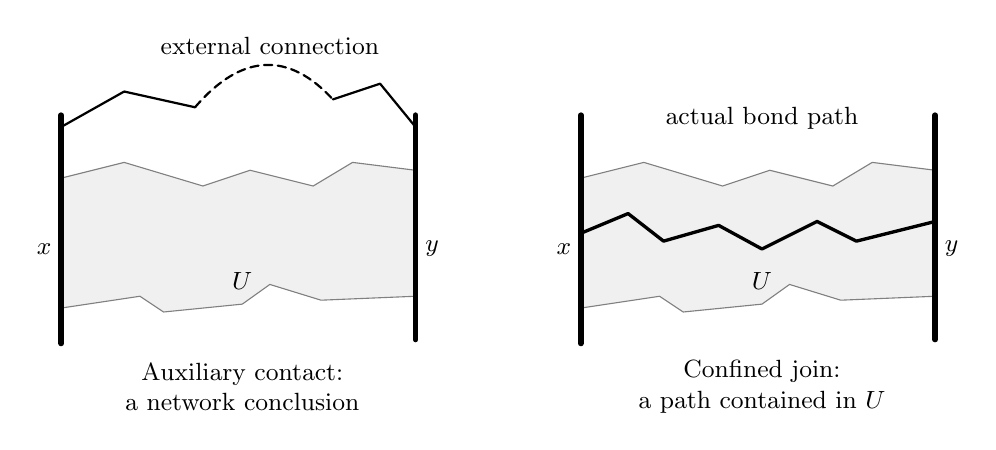
\begin{tikzpicture}[x=1cm,y=1cm,font=\small,line cap=round,line join=round]
  \foreach \shift in {0,6.6} {
    \begin{scope}[xshift=\shift cm]
      \path[fill=gray!12] (0,.75) -- (1,.9) -- (1.3,.7) -- (2.3,.8) -- (2.65,1.05)
        -- (3.3,.85) -- (4.5,.9) -- (4.5,2.5) -- (3.7,2.6) -- (3.2,2.3)
        -- (2.4,2.5) -- (1.8,2.3) -- (.8,2.6) -- (0,2.4) -- cycle;
      \draw[gray] (0,.75) -- (1,.9) -- (1.3,.7) -- (2.3,.8) -- (2.65,1.05)
        -- (3.3,.85) -- (4.5,.9);
      \draw[gray] (0,2.4) -- (.8,2.6) -- (1.8,2.3) -- (2.4,2.5) -- (3.2,2.3)
        -- (3.7,2.6) -- (4.5,2.5);
      \draw[line width=2pt] (0,.3) -- (0,3.2);
      \draw[line width=2pt] (4.5,.35) -- (4.5,3.2);
      \node[left] at (0,1.5) {$x$};
      \node[right] at (4.5,1.5) {$y$};
      \node at (2.3,1.1) {$U$};
    \end{scope}
  }
  \draw[thick] (0,3.05) -- (.8,3.5) -- (1.7,3.3);
  \draw[densely dashed,thick] (1.7,3.3) .. controls (2.3,4) and (2.9,4) .. (3.45,3.4);
  \draw[thick] (3.45,3.4) -- (4.05,3.6) -- (4.5,3.05);
  \node[above] at (2.65,3.85) {external connection};
  \node[align=center] at (2.3,-.25) {Auxiliary contact:\\a network conclusion};
  \draw[line width=1.2pt] (6.6,1.7) -- (7.2,1.95) -- (7.65,1.6) -- (8.35,1.8)
    -- (8.9,1.5) -- (9.6,1.85) -- (10.1,1.6) -- (11.1,1.85);
  \node[above] at (8.9,2.9) {actual bond path};
  \node[align=center] at (8.9,-.25) {Confined join:\\a path contained in $U$};
\end{tikzpicture}
\caption{Network contact and a confined join. The hubs $x,y$ represent
measured blockers or terminal walls, and $U$ is the untouched channel
between them. A network connection may use exterior graph portions
(left). Lemma~\ref{lem:confined-join} produces an actual open path
inside $U$ (right), under its separated-barrier, ordinary-incidence,
and planar-cap hypotheses. In a pure two-end-wire disk, network
connection already has an actual witness; the additional conclusion
here is confinement to the channel.}
\label{fig:actual-network}
\end{figure}


\subsection{Physical routing in regular geometries}

We next build prescribed physical connections from a finite chain of
crossing templates and confined joins. Free-wall attachments require
a separate seed construction. For several attachments, one further
point is essential: the local joins must belong to the same physical
component inside each shared corridor. The component estimate below
provides this compatibility before the final union bound.

All probabilities in this subsection are finite positive FK probabilities
at the fixed self-dual odds. A path called \emph{actual} uses open bonds,
including an ordinary terminal incidence when appropriate, and never
uses an identification as a path edge. Boundary incidences on different
banks of a slit remain distinct. Constants may depend on a fixed finite
collection of geometric shapes and their positive clearances. Geometric
parameters are fixed first; the mesh then tends to zero. In particular,
a positive lower bound for a fixed thin corridor need not remain positive
as its width tends to zero.

\begin{definition}[Regular collars and permitted exterior data]
\label{disk:regular-collars}
A regular radial collar is a full tile annulus or a union of a bounded
number of tile sectors separated by straight coordinate walls. The
sector angles belong to the fixed finite list of quadrant, half-plane,
three-quadrant, and slit geometries. Distinct banks and distinct corner
incidences are kept distinct. Tile-level cuts specify its two radial
sections. Designated wire intervals may run along the banks. Name every
identified bank class that meets the collar, whether it crosses the
whole collar or occupies only a partial bank interval, and suppose
their total number is at most a fixed $J$. These classes are the named
hubs of the collar; $J$ counts all of them, not just those meeting
both radial sections.

Exterior data are \emph{permitted} if they arise from finite FK graphs
with positive odds and have the following planar attachment structure.
The graph on either side meets the collar only at its own radial
section and the named hubs. It preserves all ordinary collar incidences
and designated wire portions, and has no other bank or interior
attachment. It may induce any partition on that section together with
the hubs, subject to the following residual-cap condition. In each of
the four quotients obtained by imposing neither, either, or both side
partitions, remove from the cap ledger every final class meeting a
named hub. The remaining classes must be separate noncrossing caps on
the two coordinated radial sections: place the sector strips side by
side in angular order and reverse the inner boundary order, resolving
coincident accesses in their separate fans. The two residual caps
occupy the two separate boundary arcs of this drawing.

When comparing two laws, the graph and deterministic wires on the
remote side agree; the other, unknown side may induce any permitted
partition. A rectangular bulk collar is an ordinary polygonal annulus
of fixed shape buffering a box, with positive relative width and no
internal wall. Local patches on a planar capped cylinder are permitted
only when the specified disk or sector charts satisfy this same
attachment and residual-cap contract.
\end{definition}

\begin{lemma}[The initial collar comparison]
\label{disk:initial-collars}
In the geometries of Definition~\ref{disk:regular-collars}, collars of a
sufficiently large fixed radius ratio give bounded reciprocal marginal
densities on their remote side, uniformly in the permitted unknown-side
data. The same holds in the opposite radial direction and for a fixed
rectangular bulk collar.
\end{lemma}

\begin{proof}
For a bulk collar this is Proposition~\ref{prop:annular-density}, with
polygonal cuts and ordinary buffers. For sectors, retain every named
bank class as a hub, including every partial bank interval. In each of
the four cross pressure masses entering the alternating
partition-function identity, discard terms hitting a final hub class.
Positive coverage and the singleton identity charge at most $J\log t$
for these terms, as in Lemma~\ref{lem:hub-mass}. All cap classes
absorbed into a hub are discarded with it. The residual-cap condition
in Definition~\ref{disk:regular-collars} supplies the separate
noncrossing caps on the coordinated cuts in each quotient. This is the
cap order needed by the clean comparison; the bound on $J$ alone would
not supply it.

Each complete clean sector is a tiled disk, and its blank actual radial
crossing probability is arbitrarily small at sufficiently large fixed
radius ratio, by Theorem~\ref{thm:actual-disk}. Their finite disjoint
union has the same property by a union bound. The separate-cap and
no-hit comparisons, followed by the alternating pressure identity,
therefore bound all four residual masses. This is precisely the sector
density argument, applied to the coordinated disjoint charts; adding
back the discarded hub terms leaves a uniform bound. The mixed
partition-function bound says that the relative weight of an exterior
state changes by a bounded factor when the opposite cap changes.
Summing over exterior states and normalizing proves the stated marginal
comparison. Reversing radial order makes the same proof apply inward.

If a chosen positive cap completion adds a fixed bounded number of
further block identifications, each changes every configuration weight
by either $1$ or $q^{-1}$, and these additions change normalized
densities by a bounded factor. Any additional bank class instead
retained in the collar must be included in $J$ and satisfy the same
attachment and residual-cap conditions. Thus the comparison does not
cover an unbounded collection of partial bank classes or unlisted
lateral attachments.
\end{proof}

\paragraph{Searches and their physical blockers.}
We use the physical face exploration of Lemma~\ref{sector:frontier}
in each tiled quadrilateral. Designate its end arcs as near and far,
and keep the longitudinal flank faces separate. Start from the
\emph{exterior} face of the chosen flank. An edge is queried only from
a reached complementary face; the opposite face is entered only if
the intervening tested-color physical bond is closed. In particular,
interior faces adjacent to the starting flank are not seeded for free.
The end cuts are impassable to this search. Fictitious exterior end
spokes specify only the disk separation topology: they are neither
physical path edges nor identifications in the FK law.

If an actual tested-color crossing exists, the search cannot reach
the other flank. Exhaust its reached component and temporarily set
the unqueried tested-color bonds closed. This does not enlarge the
reached component, since every edge leaving it has already been
queried and found open. The path/cut alternative therefore gives a
crossing supported on measured open bonds. Select the simple frontier
adjacent to the unsearched side by fixed tie breaks, orient it from
the near cut to the far cut, and retain the segment after its last
near-cut visit and before its first subsequent far-cut visit. Denote
this measured actual path by $P$. Its opposite-side edge interiors
and ordinary incidences remain unqueried. Temporary closure selects
the witness and imposes no additional condition on the random state.

One can require a crossing to be proper, meaning that it has no other
contact with its two end cuts. For this search, split the incidences at
an end vertex into separate leaves in fan order, ignore travel along
the end cut, and add fictitious outward terminal spokes. This changes
the search drawing, not the random states or the FK partition. A
simple trimmed physical witness gives the corresponding proper
crossing in this auxiliary drawing, even if it touches a longitudinal
wall or uses boundary bonds. At a shared wall incidence, an access
from the unsearched side meets the witness before or at that incidence.
All queries and physical paths remain in their original slot fans.
Known open diagonals serving as cutters have ordinary
half-tiles on their unqueried side; in the opposite color their new
boundary spokes are dangling or dead. Thus cutting at a measured
blocker gives free longitudinal boundary in that opposite color.

The shielding assertion is useful also in endpoint order. If a proper
witness ends before a specified opening in the far end cut, a search
from the witness's side cannot discover a frontier crossing ending
beyond that opening. Otherwise a reached complementary face incident
to its last bond could be continued inside that tile to the end cut
without meeting the witness. This contradicts separation by the
witness, which has no earlier contact with that cut. These statements
are statements in the split disk drawing, so they remain true with
boundary touches and coincident bank images.

Every successful orientation or endpoint-clearance alternative used
below is a union of leaves of its own deterministic edge exploration.
On an individual leaf, delete the queried closed edges and contract
the queried open components. Lemma~\ref{lem:finite-conditioning} gives
the exact FK law on the unqueried edges, with its induced planar
partition. Bounds on those leaves are averaged before conditioning on
any further success event. No FK law conditioned only on a union of
successful leaves is asserted.

\begin{proposition}[Actual routing and terminal attachments]
\label{prop:routing}
In a fixed regular patch with permitted planar exterior data, an actual
crossing of either color along a cleared simple corridor between two
short transverse cuts has probability bounded below by a positive
constant. The connection is confined to that corridor and small
prescribed endpoint neighborhoods. The conclusion is uniform when its
geometry has uniform positive clearances.

A terminal may instead be a continuous wire interval of the tested
color, an unwired flat wall interval, or a previously measured actual
blocker with a uniformly clear tangent-disk approach. In the last case
the blocker must be the only locally accessible obstruction from that
approach, allowing further portions of the same labeled barrier; its
ordinary unqueried incidences must be available up to the contacts.
An attachment to a measured blocker is an actual contact with that
path. An attachment to a wire requires just one actual wall contact.

Finitely many such attachments can be imposed simultaneously in the
following layouts: disjoint branch corridors arriving at spaced points
on a skinny joining tube; a four-terminal tree with two radial and two
wall branches; a ring of cleared corridors; or a corridor winding once
around a regular cylinder and returning to a distinct point of the
same joining tube. These conclusions hold conditionally on the
initial terminal exposures.
\end{proposition}

\begin{proof}
We prove the claims in an order that uses only the large-ratio collar
comparison already available.

\emph{Bulk templates and their gaps.}
The square-crossing and clipped-template construction in the proof of
the auxiliary contact lemma, Lemma~\ref{disk:auxiliary-contact}, supplies
the following finite collection of supports in a cleared corridor.
Small squares carry actual crossings between tiny selected subarcs of
two opposite sides, and clipped squares implement a right-angle bend.
Their individual conditional probabilities are positive uniformly in
planar exterior data. To recall why this is an actual-crossing input,
the square path/cut alternative gives probability at least $1/2$ for
one of a crossing and its complementary crossing. Duality, a grid
symmetry, and bounded ordinary annular marginal comparison transfer
the latter alternative to a crossing of the requested color. Splitting
the two end sides into finitely many short intervals selects endpoint
patches at a positive probability cost. Cropping a crossing gives the
clipped templates. Transfers and conditional lower bounds use ordinary
buffers around the whole support.

Here are the placement features that will be needed. Approximate the
cleared route by a simple axis-polygonal route at a fixed fine geometric
scale, erase loops, and keep positive clearance after this perturbation.
On a straight segment, pair a square template with its reflection so
that the two endpoint-center transverse displacements cancel. Adjust
the square side lengths to obtain the required axial advance. At a
right-angle turn use a square clipped by a transverse diagonal and a
reflected, traversal-reversed copy on the other side of that diagonal.
The entry and exit strips can be narrower than the bend supports, so
nonadjacent supports and their buffers are disjoint. Choose bend sizes
first. Their endpoint displacements are then fixed; two independent
axial segment adjustments absorb these displacements and all gap
lengths. This gives a fixed finite number of templates before the
final gap tolerances are chosen. Extend the first and last templates
across the desired corridor cuts and trim their crossings there.

Consecutive envelopes have tiny positive gaps between transverse end
caps and still smaller endpoint tolerances. On the event that every
template crosses, expose each extremal frontier from the same
longitudinal side of the oriented route. The exposures use disjoint
supports. Around the midpoint of a matching gap, and between radii
much larger than its width and much smaller than the template size,
the two measured blockers span an annulus in opposite open
half-planes. Their inward endpoints may be prolonged across the
innermost disk by fictitious spokes solely to specify their separation
topology. The blockers themselves are the barriers throughout the
annulus where the join lemma is applied.

The annular component on the unsearched side has no measured
incidence before it hits one of these blockers. Indeed an entry
through an envelope's unsearched flank is shielded by its frontier.
An entry through its searched flank is not in this component: that
flank has an exterior route to the other diameter ray without crossing
the blocker. At a straight cap this route goes around its lateral
edge. At a clipped bend, at the radii in question at most one lateral
corner intrudes; the cap and that side bound a wedge of fixed positive
angle, and one exits around its searched side. For a narrow normal
strip one exits around the corresponding parallel side. The two full
barrier spans separate the two rays, so none of these searched-side
entries is accessible from the focal component. This also excludes
folded measured bays. Bounded tile-rounding errors are absorbed in
the strict half-plane margins and a fixed enlargement of the radial
band. These are the hypotheses of Lemma~\ref{lem:confined-join}.

Let $S$ be the intersection of the template successes. Their disjoint
buffer estimates give $\PP(S)>0$. The successful leaves already
determine $S$. On every such leaf the probability of failure of any
specified actual join tends to zero as the gap ratio tends to infinity,
uniformly in the permitted remaining data. A finite union bound thus
joins the entire chain with positive conditional probability. Each
join is physical and confined to its prescribed patch. This proves
bulk corridor crossing without making any connection through an
external wire.

\emph{A wire or a measured tangent blocker.}
For a straight wire interval, terminate a thin bulk strip at a small
positive normal distance from the wall and expose its frontier on a
compatible side. The wall and this blocker are the two barriers for
the same confined-join argument. The resulting actual path stops at
one contact of the specified wire.

More generally let a tangent disk of radius $c'>0$ touch the measured
blocker at $z$, with the stated ordinary cleared approach. Terminate
the incoming branch at distance $\epsilon$ along the inward normal,
using a still thinner straight normal strip in a patch of radius $s'$.
Choose
\begin{equation}\label{disk:tangent-scales}
       (s')^2/c'\ll\epsilon\ll s'\ll c'.
\end{equation}
In coordinates tangent at $z$, disk exclusion confines every accessible
part of the old blocker to a half-plane enlarged by
$O((s')^2/c')$. The incoming strip is on the other side of the middle
diameter with margin of order $\epsilon$. Between an inner radius
larger than the gap and an outer radius smaller than $s'$, both
barriers span the annulus in opposite half-planes. Only the specified
blocker label is accessible at the old wall. Applying the confined
join therefore makes an actual attachment to the measured path, with
failure arbitrarily small. The hierarchy in
\eqref{disk:tangent-scales} is chosen before the mesh limit. Cleared
routes and tangent normals in a compact family admit uniform choices,
by a finite pixel approximation of their interior routes, or by taking
a position limit and retaining strict sub-clearances.

\emph{A free-wall seed.}
Consider first a blank tested-color law in a flat half-box. A small
central wall interval has positive probability of an actual arm to
the opposite line. To see this, separately wire that interval and
the opposite line. Lemma~\ref{disk:auxiliary-contact} gives a positive
two-terminal probability. With only these two wires, network
connection is equivalent to an actual path between the two sets:
erase all visits to an end wire before the last departure and after
the first arrival. The no-hit comparison of Lemma~\ref{lem:no-hit}
makes the blank actual probability at least this pure probability.
Denote a resulting lower bound by $p_0>0$.

Put a protected wall rectangle around the central interval, with a
fixed positive lateral margin $a$. An arm going to the opposite line
either reaches height $\eta$ within that rectangle or exits it
laterally while staying below height $\eta$. Choose many disjoint
boxes of dimensions comparable to $\eta$ along either possible
lateral exit route. In each, the opposite color, which is wired on
this wall, has an actual transverse arm from the wall to above height
$\eta$ with conditional probability at least $c_1>0$. This is the
already proved wired-wall construction in a fixed shape. These arms
block the tested-color lateral excursion. With at least
$c_2a/\eta-O(1)$ tests, its probability is at most
\[
  2(1-c_1)^{c_2a/\eta-O(1)}.
\]
Choose $\eta>0$ so this is less than $p_0/2$. The protected actual
wall-to-height event then has probability at least $p_0/2$.

Choose the wall-seed scales small compared with the available straight
wall patch. The protected rectangle can then be surrounded by a
half-sector collar of the sufficiently large fixed ratio in
Lemma~\ref{disk:initial-collars}, inside the original flat patch. This
transfers its positive probability to every permitted exterior with
the same free tested-color wall. Expose an extremal seed inside its
protected rectangle, stopping at a fixed height below the height just
obtained. The region above that cut is untouched. Its endpoint
determines an incoming approach from that region; the branch is
chosen after observing the seed. At the much smaller attachment scale
the cut is a straight transverse cap, including the one-corner wedge
case if the endpoint lies at a lateral corner. Choosing the compatible
exposed side of the incoming branch gives the gap geometry already
checked. A confined join attaches to the physical seed, which in turn
is physically connected to the unwired wall. Notice that this argument
has used large-ratio sector comparison only. Thin-ratio comparison
will be deduced after the physical screens have been constructed.

\emph{Traversals in one physical component.}
Two attachment searches can select different traversals of the same
corridor. We therefore need the following claim before combining the
attachments. Let $C$ be a branch corridor or joining tube with whole
end cuts $A_C,B_C$, let $E_C$ be its actual traversal event, and let
$U_C$ be the event that all its proper actual traversals lie in one
physical component supported in $C$. Put
\[
 \alpha_C=
 \frac{1+\max\{\operatorname{diam} A_C,
                    \operatorname{diam} B_C\}}
      {\operatorname{dist}(A_C,B_C)},
\]
with lengths in tile units. The claim is
\[
 \PP(U_C^c\cap E_C)\le o(1)\PP(E_C)
 \qquad\text{as }\alpha_C\longrightarrow0,
\]
uniformly in permitted exterior data, including fixed states in
disjoint supports. Narrow end cuts and then fine mesh make
$\alpha_C$ small in our fixed layout.

To prove the claim, expose the two extreme frontiers toward the
middle. Their successful leaves determine $E_C$. Every other
traversal disconnected from them must
lie between them, since a traversal farther toward either searched
side would shield the corresponding measured frontier from that
search. If the frontiers are disjoint, the disk between them has
unqueried interior and free opposite-color longitudinal flanks. Its
possible extra identifications are planar joint end caps. Failure of
an actual join between the frontiers in this disk forces an actual
opposite-color traversal between its end arcs. The latter has
probability $o(1)$, uniformly on these leaves, by
Theorem~\ref{thm:actual-disk}, because its two ends are subarcs of
$A_C,B_C$ and have separation ratio tending to infinity with
$\alpha_C^{-1}$. A transverse actual join intersects
every proper traversal between the two frontiers. If the frontiers
intersect, shielding already excludes a traversal disconnected from
both. Boundary contacts are separated in their own fans; the
half-tile convention along a known open cutter makes precisely the
free opposite-color boundary used in this application. The failure
bound holds on each successful pair of frontier leaves. Averaging
those leaves proves the displayed relative estimate.

\emph{Simultaneous attachments.}
Place a long skinny joining tube of half-width $w$ in the clear middle.
Draw nonintersecting buffered branch corridors to spaced points along
its length. Near a top arrival a branch stays above transverse
coordinate $2w$ and ends in a thin normal strip; bottom arrivals are
reflected. Their distant ends have the already specified terminal
geometry. All corridor and tube success events have jointly positive
probability by successive conditional lower bounds. Denote their
intersection again by $S$. We will bound physical failures conditional
on $S$ by first obtaining uniform bounds on exploration leaves that
decide $S$ while leaving the relevant join region unqueried.

For corridor $j$ let $U_j$ be the physical event that all its proper
traversals belong to one component within it. For attachment $i$ let
$J_i$ be the physical event that a local path joins some successful
traversal in each of its two incident supports, or attaches one such
traversal to the indicated terminal blocker or wall contact. To bound
$J_i^c$, explore just the pertinent frontiers from the sides suitable
for that attachment and fix the other disjoint support states away
from its patch. The fixed outside states decide the successes of the
other supports; the frontier leaves decide those of the two incident
supports. Thus each retained combined record decides $S$, and its
unqueried join region has the ordinary conditional FK law. At a top
tube arrival, search the tube from its bottom lip.
Its whole frontier is below height $w$. Center the separating
horizontal diameter in the gap above it; both focal directions above
the tube are available, and select the one exposed by the branch
search. The tube has two continuations with its same label, as allowed
in Lemma~\ref{lem:confined-join}. The previous cap and tangent arguments
handle the other terminals. Hence for any prescribed $\varepsilon>0$
the fixed geometries can be chosen so that the failure bound is at
most $\varepsilon$ on every retained record. The component claim
gives the same conclusion for $U_j^c$ by using that corridor's two
frontiers and fixing the other supports. Averaging each experiment
separately gives
\[
 \PP(J_i^c\cap S)\le\varepsilon\PP(S),\qquad
 \PP(U_j^c\cap S)\le\varepsilon\PP(S),
\]
and hence
\begin{equation}\label{disk:conditional-joins}
 \PP(J_i^c\mid S)\le\varepsilon,\qquad
 \PP(U_j^c\mid S)\le\varepsilon.
\end{equation}
For $k$ attachments and $m$ corridors it follows that
\begin{equation}\label{disk:physical-union-bound}
 \PP\left(\bigcap_{i=1}^k J_i\cap
                 \bigcap_{j=1}^m U_j\,\middle|\,S\right)
       \ge 1-(k+m)\varepsilon.
\end{equation}
On this event all the selected attachments belong to the intended
physical components. Different attachments may require different
orientations of the same exploration: the estimates are for the
physical events $J_i$, so their explorations need not coexist. The
error bound remains $\varepsilon$ even when $\PP(S)$ is small.

For clarity, choose the fixed finite layout and its mutual clearances
first, then the join patches and required radial ratios, then the
narrow strip and endpoint tolerances, and finally the mesh. At a
tangent terminal shrink its patch further to satisfy
\eqref{disk:tangent-scales}. With
$\varepsilon<1/(2(k+m))$, \eqref{disk:physical-union-bound} proves
the desired positive probability. All its paths use just the corridors,
their small join neighborhoods, and the measured terminal blockers.

A four-terminal tree is obtained by two opposite-side wall branches
at spaced central tube positions and two radial branches at its
longitudinal portions. A ring uses a finite cyclic chain of corridors.
On a cylinder choose a simple winding corridor with separated ends
at two distinct tube positions. Its actual traversal, joined at both
ends to the connected tube, gives a closed walk with nonzero winding
number: the tube return lies in a disk and the corridor winds once.
Deleting contractible loops from that walk leaves a noncontractible
actual cycle. This finishes all the asserted layouts.
\end{proof}

\begin{proposition}[Actual screens]
\label{prop:screens}
For each fixed regular collar geometry, either color has an actual
wall-to-wall screen in a sector, or an actual surrounding circuit in
a full annulus, with a uniformly positive conditional probability
under permitted exterior data. The paths remain in a prescribed
middle subcollar and meet every designated continuous through wire
of the tested color when those are present. The statement includes straight walls,
quadrant and reentrant corners, slit tips, and differing wire
designations on the banks near a flip. Contacts are chosen on
straight bank patches separated from the tip or corner apex.
Different colors in tile-disjoint sectors can be required together.
\end{proposition}

\begin{proof}
Choose bank patches away from the finitely many apexes and draw a
cleared transverse route in each sector. Use a wire contact or a
free-wall seed according to the color designated on that bank.
Proposition~\ref{prop:routing} constructs the entire actual screen.
For an annulus, use the ring layout around its inner boundary; its
closed actual walk contains a surrounding simple circuit. For a
finite collection of disjoint sectors impose the specified screens
successively, conditioning on the other support states; each retained
law still has the permitted planar exterior data. The product of
the finitely many positive lower bounds is positive. Distinct slit
banks are treated in their own charts, so physical coincidence does
not join their incidences. No path in this construction uses a wire
as an edge.
\end{proof}

\begin{lemma}[Fixed-ratio sector comparison]
\label{disk:thin-collars}
Lemma~\ref{disk:initial-collars} holds also for a fixed smaller
nontrivial sector ratio, with a constant depending on that ratio and
the fixed geometry.
\end{lemma}

\begin{proof}
First consider the clean disjoint union of sectors, without bank
hubs. In its blank tested-color law, an actual opposite-color screen
in each component blocks radial traversal. Under duality the opposite
color has the requisite wired wall conditions, and
Proposition~\ref{prop:screens} applies conditionally. Thus the blank
actual radial probability $b$ satisfies $b\le1-\eta_0$ for some
$\eta_0>0$.

The blank cross pressure mass $\Delta$ is bounded as well. Cover one
radial cut by finitely many small interval patches, of diameter tiny
compared with the collar depth. For a patch in one component the
pure connection probability to the other entire cut is arbitrarily
small by Theorem~\ref{thm:pure-disk}; all other components attach
only to the latter full wire and do not change this test. The
one-sided density estimate bounds the pressure mass for this pair.
Positive coverage and the finite patch cover bound $\Delta$ for
the full two cuts. The cofacial one-sided comparison gives the
corresponding bound after either single cap is imposed.

Write $Z_{ab}$ for the four cap choices, and $\Delta_{ab}$ for
their cross masses. The alternating identity reads
\[
 \log\frac{Z_{11}Z_{00}}{Z_{10}Z_{01}}
       =\Delta_{10}+\Delta_{01}-\Delta_{00}-\Delta_{11}.
\]
The blank no-hit mixed-gain bound, using $b\le1-\eta_0$, supplies
a lower bound for the logarithm. Nonnegativity and the three bounds
just proved therefore bound $\Delta_{11}$ and the mixed logarithm
in both directions. This proves bounded reciprocal densities for
the clean union. Discarding all at most $J$ named bank-hub
classes and retaining the coordinated residual noncrossing caps,
exactly as in Lemma~\ref{disk:initial-collars}, proves the general
statement. The proof uses the physical screens only here, after
their construction; the wall seeds used only the earlier large-ratio
comparison.
\end{proof}

\subsection{Relative localization through restricted collars}

Bounded density comparison preserves a positive probability but does
not make distant boundary data negligible. A screen that meets every
possible through wire removes that dependence altogether on a fixed
positive part of the collar law. Repeating this common part, and
retaining one final bounded comparison, gives a relative error for
every nonnegative observable, including rare events.

\begin{proposition}[Relative collar comparison]
\label{prop:relative-collars}
Consider two finite positive FK laws at the fixed $q$, with ordinary
collar bonds, whose graphs and deterministic wires agree on the remote
side of a sequence of regular collars and whose unknown-side data are permitted in the sense of
Definition~\ref{disk:regular-collars}. Require each collar to have
one of the following geometries:
\begin{enumerate}[label=(\roman*)]
\item a full annulus with no named bank hubs, or one sector whose only
bank attachments are continuous primal wire portions along its two
side rays, crossing the collar and each met by its primal
wall-to-wall screen;
\item two sectors, with only such screen-met continuous primal wire
portions on both side rays of one sector, no bank or hub attachment in
the other, and no direct contact between the sectors inside the collar.
Side graphs may join contacts of the two sectors only through the
corresponding permitted radial cap.
\end{enumerate}
After $m$ further collars of a sufficiently large fixed ratio and
one final comparison collar, the expectations of any fixed
nonnegative function $f$ supported beyond them satisfy, for fixed
$C\ge1$ and $0<c<1$, the two inequalities
\begin{equation}\label{disk:relative-density}
 \begin{split}
 \EE_1 f&\le\bigl[1+(C-1)(1-c)^m\bigr]\EE_2 f,\\
 \EE_2 f&\le\bigl[1+(C-1)(1-c)^m\bigr]\EE_1 f.
 \end{split}
\end{equation}
They are understood in the extended nonnegative reals. For finite
positive expectations they imply
$\EE_1 f/\EE_2 f=1+O((1-c)^m)$, and the expectations vanish together.
The constants are independent of the far graph, the unknown-side
partition, and $f$. The same conclusion holds in the reverse radial
direction and after a positive finite tilt supported on the unknown
side. In particular, unknown-side changes may join or separate the
designated wire portions. The contraction requires the enumerated
screen-met attachments; the general bound on $J$ in
Definition~\ref{disk:regular-collars} alone is not sufficient for it.
\end{proposition}

\begin{proof}
We give the finite FK comparison and coupling argument. It also explains
the restrictions on the geometry. Throughout a comparison, keep the
entire common graph beyond the current section fixed, including its
far boundary data. Collar marginals can depend on this remote graph;
all constants below are uniform in that dependence.

Split each designated wire transversely
at a section, retaining its connections separately on either side
and one representative of the possible through connection. There
are only boundedly many such representatives. The unknown graph
then enters the common graph as a permitted partition $\xi$ on that
section, with all the common deterministic wire pieces included.
Any bounded extra split or merger has weight ratio between
$\min(q,q^{-1})$ and $\max(q,q^{-1})$ per operation. The bounded
collar comparison therefore applies equally to this representation.

Use a sufficiently large fixed ratio, for example enlarge a factor
$256$ further if needed, to leave two buffered subcollars at every
step. Fix a reference permitted partition. The initial comparison
subcollar makes the marginal $\mu_\xi$ on the second subcollar
dominate $K^{-1}\mu_*$ for every $\xi$, with a constant $K$ and
the same reference marginal $\mu_*$. This is a pointwise inequality
of finite measures on the subcollar edge configurations.

Inside that second subcollar, in case (i) require a primal circuit,
or a primal wall-to-wall screen meeting every named primal bank wire.
In case (ii) require a primal screen in the wired sector and a dual
screen in the other. Proposition~\ref{prop:screens} gives a reference
probability at least $p_*>0$ for this event $G$. On $G$, the partition
transmitted to the next section is determined by the common
subcollar configuration alone. Indeed every connection from the
unknown side to the remote side in a screened primal component must
meet a connected primal screen. All named bank wires there
already meet that same screen. Connections through the unknown
region can therefore make no further distinction among its remote
contacts. In the unwired second sector the dual screen allows no
actual primal crossing, and there is no bank or hub attachment to bypass it.
The absence of other intersector contacts is used at exactly this
point.

Any cluster of the common subcollar meeting the next section but
avoiding the transmitting screen is therefore unable to acquire
an extra connection through the unknown region. Components wholly
on the exposed side contribute factors independent of all remote
states and cancel when the conditional law is normalized. By the
finite domain Markov identity, the entire conditional remote law
thus depends only on this transmitted partition.

For completeness, screens can be discovered without querying edges
strictly beyond them. Explore complementary-color components from
the unknown-facing section. If the screen exists, the search stops
short of the remote section; otherwise the disk path/cut alternative,
or its annular version, would give a complementary crossing. The
measured frontier consequently contains a blocking physical path or
circuit. Perform this search in the buffered middle and reverse
colors in the unwired sector. Thus the same transmitted-partition
description applies either by revealing the whole fixed subcollar
or by stopping at its measured screens.

To specify the transition precisely, reveal the tile states up to the
next section and let $\eta$ be the partition they induce there from
the exposed side, together with the common deterministic wire pieces.
The planar drawing and the absence of unlisted lateral attachments
keep $\eta$ in the permitted class. Conditional on the exposed states,
the law of the fixed remote graph is the FK law with partition $\eta$,
by Lemma~\ref{lem:finite-conditioning}. Thus, for a remote observable
$f$, its conditional expectation is a function $g(\eta)$ of that
partition. On the screen event $G$, the preceding separation argument
shows that $\eta$ is determined by the second subcollar configuration
alone and is independent of the entering partition $\xi$. Away from
$G$ it may also depend on the first subcollar and on $\xi$.

The measure
\[
        \lambda=K^{-1}\one_G\mu_*
\]
is a common submeasure of all second-subcollar laws and has mass at
least $p_*/K$. On its support the just-defined map to $\eta$ is common
to all entering partitions. Its pushforward is therefore a common
submeasure $\nu$ of the laws $L_\xi$ of the induced next partition,
with the remote graph still held fixed. These laws are the transition
kernels used below. Choose a fixed $c>0$ not exceeding
$p_*/K$, and reduce $\nu$ to mass $c$ if necessary. Every such
kernel has the form
\begin{equation}\label{disk:collar-minorization}
       L_\xi=c\widehat\nu+(1-c)\widetilde L_\xi,
\end{equation}
where $\widehat\nu$ is the same probability measure for all
$\xi$. This is the common positive part of a coupling. No
stochastic monotonicity of FK boundary conditions is required.

For a bounded nonnegative $f$, make the relative-error deduction explicit.
Number the sections
$0,1,\ldots,m$ toward the support of $f$ and reserve the final
bounded-comparison collar beyond section $m$. Let
$[a_j,b_j]$ be the range of conditional expectations of $f$ over
all permitted partitions at section $j$, including the common
remaining graph. Conditioning on the next section gives
\[
 [a_j,b_j]\subseteq[a_{j+1},b_{j+1}],\qquad
 b_j-a_j\le(1-c)(b_{j+1}-a_{j+1}),
\]
where the second assertion follows from
\eqref{disk:collar-minorization}. The last comparison collar gives
$b_m\le C a_m$. If $a_m=0$, then $b_m=0$ and all expectations
vanish. Otherwise $a_0\ge a_m>0$ and
\[
 \frac{b_0-a_0}{a_0}
 \le (1-c)^m\frac{b_m-a_m}{a_m}
 \le (C-1)(1-c)^m.
\]
It follows that either expectation is at most
$[1+(C-1)(1-c)^m]$ times the other. This proves
\eqref{disk:relative-density} for bounded $f$. For a general
nonnegative $f$, apply those two inequalities to $f\wedge M$ and let
$M$ increase by monotone convergence. No quotient of infinite
expectations is used.

The same proof works inward, using the reversed collar comparison
and the same separation by actual screens. A positive modification
on the unknown side merely changes the mixture over its induced
partitions: every member has the same common submeasure and lies
in the same interval $[a_0,b_0]$. Integration over that mixture
proves the assertion about tilts. In particular no fixed connection
through a gap has to be retained when the gap belongs to the unknown
region. In case (ii) this is why both colors of screen, rather than
only the screen meeting the primal wires, are required.
\end{proof}

\subsection{Relative arm splices and an opposite-arm loss}

The remaining construction preserves a specified arm event while
joining its truncated pieces through a fresh window. Its probability
must be compared with that of the original arm, which may be very
small. A finite cover by one-sided exploration successes supplies this
relative comparison; the reconstruction also inserts a transverse
screen when an opposite-color radial arm must be excluded.

\begin{lemma}[A flat splice and strict opposite-arm cost]
\label{lem:relative-arm}
Let $A$ require an actual radial traversal of a specified color in a
long regular half-annular region whose two longitudinal walls carry
the continuous portions of a flat mixed-color boundary condition.
The start is a full inner cut or a specified flip-gap vertex and
the target is a full outer cut. Choose mutually separated marker
bands, with broad fixed-proportion splice windows on both sides of
each marker. Let $B_i$ require an actual opposite-color radial
traversal of marker $i$. There is $c>0$, depending only on the fixed
window shapes, such that
\begin{equation}\label{disk:opposite-arm-loss}
 \PP\left(A\cap\bigcap_{i=1}^k B_i\cap E\right)
 \le (1-c)^k\PP(A\cap E)
\end{equation}
whenever the extra requirement $E$ is supported outside those
windows. The estimate is uniform under permitted exterior
conditioning. A separated short arm can be included in $E$.

For the splice conclusion, let $T$ be the joint event of two
same-color actual arms, each supported in one of the two disjoint
side domains from its prescribed source to a full cut on its side
of a fixed-ratio window. Assume the same regular half-annular
geometry and fixed positive buffers as above, with two spaced
openings away from the flanks on each cut. Each source lies on the
opposite radial end of its side domain; a flip-gap tip is allowed
as an inner end. In units of the window scale, the distance from
the source to its window-facing cut is bounded below by a fixed
positive constant, and a side band of fixed positive depth adjoining
that cut is free of previously fixed far data. If $A_{\mathrm{join}}$
is the event that these sources are joined by an actual path in
the union of the side domains and the window, then
$\PP(A_{\mathrm{join}})\ge c\PP(T)$, uniformly under permitted
exterior conditioning. A single arm can be extended through
a further fixed-factor collar with a fixed relative probability.
Iteration gives polynomial arm lower bounds in these regular
geometries, and opposite-color screens give a strict power upper
bound for one-arm probabilities.
\end{lemma}

\begin{proof}
Fix one marker, write $B$ for its opposite-color traversal, and
condition on the edge states $F$ outside its broad window. Other
marker constraints and $E$ are thereby decided. Trim any witness
for $A$ at two cuts lying just inside the window on its respective
sides of the central marker. It gives actual paths from the two
required sources to these cuts in disjoint side domains. A source
can include a previously measured physical continuation through
$F$, but no search follows a wire identification as a path edge.

At each near cut choose two small, spaced opening intervals away
from the flanks and corners. Orient each witness toward its target
cut and retain the portion after its last source-set visit and before
its first subsequent target-cut visit. Every resulting endpoint is
a fixed positive distance to one side of at least one opening.
Run a complementary search from that endpoint's side, treating
previously fixed far states as known data. The shielding argument
given before Proposition~\ref{prop:routing} makes its measured
frontier end on the same side of the selected opening. In
particular that opening is on its unqueried side with a uniform
margin. There are only a bounded number of choices of opening and
orientation at each end. Let $T_1,\ldots,T_N$ be the corresponding
two-search success alternatives. They satisfy
\begin{equation}\label{disk:truncated-cover}
       A\subseteq\bigcup_{i=1}^N T_i
\end{equation}
for each fixed $F$, with $N$ independent of mesh and scale. On each
successful leaf retain the simple actual frontier $P$ connected
physically back to its required source. Each $T_i$ is a union of leaves
of its own pair of searches, performed in the two disjoint side
domains. The uninspected regions have their usual conditional FK laws
on individual leaves; we do not condition those laws on the union in
\eqref{disk:truncated-cover}.

We verify the uniform tangent access needed to reconstruct between
the two frontiers. From the empty central region enter a chosen
opening, then move a small fixed radial distance into its side
band and along a level transversal toward the searched flank.
This route must meet $P$: the source-to-cut crosscut separates the
opening side from that flank. Start at a fixed clear point in the
central region, and choose a clearing radius $a$ smaller than its
boundary distance, the opening separation, and all side-band margins.
Move a center from that point along the route until its first distance-$a$
approach to $P$. The resulting disk is empty and tangent to $P$.
On entering the opening its endpoint is excluded by the angular
margin; along the transverse portion it is excluded by the radial
depth. Both cuts, all fixed far data, and the other flank stay at
larger fixed distances. Any approachable point of the searched
flank is screened by $P$, or is itself a contact with $P$. Hence
there is no other locally accessible wall before the tangent
contact. The unqueried incidences up to it are ordinary. Both endpoints
of $P$ lie outside a fixed enlargement of the contact neighborhood by
the cut margins, so both branches of $P$ continue out of it. Folds behind $P$
do not affect this disk. Tile rounding is absorbed by decreasing
the chosen fixed margins. This verifies all the measured-terminal
hypotheses of Proposition~\ref{prop:routing}, uniformly in the
successful leaves. Perform the same construction at the other end.

In the clear center of the marker put a skinny tube. Two separated
branches go to the tangent approaches just obtained; two further
branches go to the two walls, with their attachment sites spaced
on opposite tube sides. Use a wired contact or the free-wall seed
as required by each wall's tested-color designation. Seed
rectangles are disjoint protected patches, exposed first. The
radial branch detours remain in their respective radial
neighborhoods, while the wall-to-wall portion remains wholly
inside the marker. The four-terminal layout of
Proposition~\ref{prop:routing} consequently has a uniform positive
conditional probability $c_0$ on every successful leaf. It both
joins the two physically source-connected frontiers, preserving
$A$, and contains a same-color wall-to-wall screen inside the
marker. The screen excludes $B$ by planar path/cut separation.

Here is the relative, rather than merely absolute, estimate.
Integration over the leaves of any fixed alternative gives
\begin{equation}\label{disk:relative-reconstruction}
 \PP(A\cap B^c\mid F)\ge c_0\PP(T_i\mid F)
       \qquad(1\le i\le N).
\end{equation}
Take the largest of these right sides and use
\eqref{disk:truncated-cover}. It follows that
\[
 \PP(A\cap B^c\mid F)
       \ge\frac{c_0}{N}\PP(A\mid F),\qquad
 \PP(A\cap B\mid F)
       \le\left(1-\frac{c_0}{N}\right)\PP(A\mid F).
\]
Thus truncated success is used as an upper cover of the original
arm event; it need not already imply that event. Averaging in $F$
while retaining the exterior requirements and iterating over the
separated windows proves \eqref{disk:opposite-arm-loss} with
$c=c_0/N$.

For the two-arm event $T$ in the statement, use the same
opening and tangent constructions and join their two radial
branches in the clear middle. No transverse screen is required.
The two-success alternatives cover the separately required arms,
and the identical bounded-union calculation gives the fixed
relative probability. For extension of a single arm use one
truncated search and one new outer terminal. The constants are
uniform in the fixed rescaled geometry. Starting at a bounded
number of mesh steps, a specified finite physical path has a
positive conditional probability depending only on that bound
and the fixed $q$. Multiplying a fixed positive extension factor
over $O(\log(R/r))$ collars gives a polynomial lower bound.
For an upper bound, separated fixed-ratio bands have conditional
probability bounded below of an actual opposite-color screen by
Proposition~\ref{prop:screens}. An actual arm avoids every such
screen. There are at least $a\log(R/r)-b$ tests for fixed $a>0$ and
$b<\infty$, so successive conditioning gives an upper bound
$(1-c')^{a\log(R/r)-b}\le C(r/R)^{c''}$ for some $c''>0$.
These estimates require no independence
of the successive bands.
\end{proof}

The cylinder application keeps a short arm near a boundary mark and
a separate long arm farther out. Small conditioned endpoint boxes
lie in the gap between them. Comparing this joint two-piece event
across the boxes' buffers avoids conditioning on a rare completed
arm. A fresh splice then crosses the gap and attaches the arm to a
winding cycle. The opposite-color marker windows are placed along
the long piece, away from all conditioned boxes and both splice
constructions.

\begin{corollary}[The grouped cylinder splice]
\label{disk:grouped-cylinder}
Let $\mathcal C$ be a finite tiled cylinder of circumference comparable
to $n$, with finite positive FK cap graphs drawn planarly at its rims.
Its bottom has a flat mixed-color boundary near a specified flip-gap
vertex $s$, and a second marked bottom point $t$ at distance comparable
to $n$. All tiles in the following charts are ordinary. Fix their shape
and buffer constants first, then take $n/r$ sufficiently large and
$r$ sufficiently large in tile units.

There are finitely many endpoint boxes in the bulk near $s$, with
distances from $s$, depths from the bottom, and mutual spacings between
fixed positive multiples of $r$. Their radii are at most $\delta r$,
where $\delta>0$ is fixed sufficiently small. Each box has a disjoint
ordinary bulk-annular buffer, of fixed relative width, within the
scale-$r$ half-disk. Choose $c_0>0$ and $C_0<\infty$ so that these
buffers lie strictly between radii $c_0r$ and $C_0r$ about $s$, with
fixed positive margins. Their complement in this gap contains the
clear two-arm splice layout of Lemma~\ref{lem:relative-arm}.

Choose fixed $0<c_1<c_2$ so that the $s$-centered half-disk of radius
$c_2n$ is an injective flat cylinder chart. The half-sector collar
between its tile-level cuts at $c_1n$ and $c_2n$ has a sufficiently
large fixed ratio for Lemma~\ref{disk:initial-collars}. The $t$ box,
of radius at most $\delta n$, and the remote middle region lie outside
the $c_2n$ chart with positive $n$-scale margins. The attached graphs
at this chart and at every endpoint buffer satisfy
Definition~\ref{disk:regular-collars}, with a fixed bound on all named
bank classes and its residual-cap condition. In particular the graph
outside the $s$ chart attaches only at its outer radial cut and those
named hubs. A regular bulk window before the $t$ box and the middle
contains a joining tube and a cleared corridor winding once between
two distinct tube positions, as in Proposition~\ref{prop:routing}.
For each of two spaced flat openings on the $c_1n$ target cut, a
cleared branch joins its outward ordinary neighborhood to the tube.
The branch and winding buffers have fixed positive $n$-scale
clearances from the conditioned regions and satisfy the permitted
local-chart contract.

Let $\mathcal D$ specify the edge states in the endpoint boxes, the
$t$ box, and the remote middle; consider any feasible value of these
data. Let $R_{\mathrm{arm}}$ be the intersection of a short actual
gap arm from $s$ to radius $c_0r$ and a separate same-color actual
radial traversal from radius $C_0r$ to radius $c_1n$, both in the
flat half-disk chart. Their supports avoid all the endpoint buffers.
Choose a finite positive FK reference cap law that agrees with the
cylinder law on the graph, odds, and deterministic wall portions
through radius $c_2n$, including the endpoint buffers, and whose
exterior at that cut is permitted. Let $A_{\mathrm{ref}}$ be its full
actual gap arm from $s$ to a fixed full cutoff of radius comparable
to $n$ and strictly beyond $c_1n$, with a fixed buffer. Put
\[
 p_{\mathrm{ref}}:=\PP_{\mathrm{ref}}(A_{\mathrm{ref}}).
\]
The cutoff separates $s$ from the outer continuation of the reference
chart, so trimming gives $A_{\mathrm{ref}}\subseteq R_{\mathrm{arm}}$.
Let $E$ require an actual arm from $s$ joined to a noncontractible
actual cycle in the stated bulk window. There is $c>0$ such that
\begin{equation}\label{disk:grouped-cycle-lower}
 \PP(E\mid\mathcal D)
    \ge c\PP(R_{\mathrm{arm}}\mid\mathcal D)
    \ge c^2 p_{\mathrm{ref}}.
\end{equation}
For $k$ mutually separated opposite-color marker-traversal
requirements $B_1,\ldots,B_k$, with their full splice windows
between radii $2C_0r$ and $c_1n/2$, one also has
\begin{equation}\label{disk:grouped-marker-upper}
 \PP\left(R_{\mathrm{arm}}\cap
                  \bigcap_{j=1}^k B_j\,\middle|\,\mathcal D\right)
 \le C(1-c)^k\PP(R_{\mathrm{arm}}\mid\mathcal D).
\end{equation}
Here $C=1$ is possible when every listed marker has its full
window; the constant permits omission of boundedly many end
markers. The constants depend on the fixed buffer choices and
reference cutoff, but not on $r,n,k$ or the values of $\mathcal D$.
\end{corollary}

\begin{proof}
Write $\mathcal D_{\mathrm{out}}$ for just the $t$-box and middle data.
First remove the conditioning in the endpoint boxes one at a time.
Each disjoint bulk-annular buffer separates that box from the entire
support of $\one_{R_{\mathrm{arm}}}$. The inward or outward bounded
comparison of Lemma~\ref{disk:initial-collars}, while holding all
other data fixed, compares a specified box state with the mixture over
its states. The number of boxes is fixed, so
\[
 \PP(R_{\mathrm{arm}}\mid\mathcal D)
 \ge c_0'\PP(R_{\mathrm{arm}}\mid\mathcal D_{\mathrm{out}}).
\]
Next apply that lemma inward across the $s$-centered half-sector
between $c_1n$ and $c_2n$. The remaining cylinder law and the
reference law agree on its inner side, including the now unconditioned
endpoint boxes. The $t$ and middle states change only its permitted
outer partition, with every bank class included in the named bound.
Consequently
\[
 \PP(R_{\mathrm{arm}}\mid\mathcal D)
   \ge c\PP_{\mathrm{ref}}(R_{\mathrm{arm}})
   \ge c\PP_{\mathrm{ref}}(A_{\mathrm{ref}})=c p_{\mathrm{ref}}.
\]
Both comparisons use the single joint observable
$\one_{R_{\mathrm{arm}}}$. In the fixed-ratio gap about scale $r$,
these requirements force the
two truncated successes used in the splice proof. The finitely
many small separated endpoint patches can be avoided by disjoint
interior bulk routes with fixed rescaled clearance; take the patch
radii small before fixing these routes. Apply the two-arm splice
and its bounded-alternative relative deduction. This constructs
the extended physical arm with a fixed fraction of the probability
of $R_{\mathrm{arm}}$.

Search this extended-arm event afresh at the $c_1n$ target cut,
using its two stated openings. The one-sided truncated search gives
a frontier with an untouched opening and tangent approach exactly as
in Lemma~\ref{lem:relative-arm}. Use that opening's cleared branch
to attach the frontier to the joining tube, then use the stated
corridor winding between its two tube positions. The winding layout of
Proposition~\ref{prop:routing} supplies an actual noncontractible
cycle in the same actual component as the arm, with a uniform
conditional probability on each successful leaf. The truncated
cover argument again turns this into a relative lower bound for
the extended-arm event. Combining the two fixed losses gives the
first inequality of \eqref{disk:grouped-cycle-lower}.

Choose a fixed large spacing ratio for the intermediate markers,
leaving their splice windows disjoint and separated from the two
endpoint constructions. A maximal regularly spaced family has
size proportional to $\log(n/r)$ up to a bounded additive error. Apply
\eqref{disk:opposite-arm-loss} to the outer radial traversal
appearing in $R_{\mathrm{arm}}$, retaining its separated short
gap arm, $\mathcal D$, and all previously decided marker
requirements in the exterior conditioning. The marker windows
lie strictly inside this outer traversal domain. This proves
\eqref{disk:grouped-marker-upper} directly for
$R_{\mathrm{arm}}$; it does not require conditioning on the
subsequent successful extension or cycle construction.
\end{proof}

\section{Passage moments and angular transfer}\label{sec:angular}

The actual-path disk estimate of Theorem~\ref{thm:actual-disk} first
gives all exponential moments for raw passages. These moments control
local nest weights and yield a strict cost gap at a flat change of wire
color, at the fixed target parameter $0<q<1$.

The second part isolates two angular decay powers in finite-circle
transfer matrices. This calculation is valid throughout $0<q<4$ and
uses no geometric probability estimate or infinite-volume law. Its
physical interpretation, together with the nest costs, will supply the
current and charge estimates in Section~\ref{sec:physical}.

\subsection{Raw passage moments}

The estimates in this subsection concern the finite switch drawing:
raw strands follow switches and stop at wall ports.  In particular,
neither a strand nor an actual crossing may use an exterior
identification as an edge.  All conditional laws below are obtained by
fixing exterior states in one of the regular buffered geometries of
Section~\ref{sec:disks}; their induced compatible boundary partitions
are allowed to vary.  In every comparison of exterior completions,
the local patch, its fixed buffer, and the continuous designated wire
portions on its walls agree.  Exterior data have the permitted planar
realizations of Definition~\ref{disk:regular-collars}.  For the bounded
collar comparisons used here, a fixed number $J_{\mathrm{bank}}$ bounds
every designated bank-wire class meeting a collar, including a class that
ends inside it.
After those classes are removed, the residual rim caps are separately
noncrossing.  No other identification bypasses the buffer.  Constants may
depend on this fixed inventory of bank classes.

\begin{convention}[Fixed geometry before small mesh]
\label{angular:mesh-convention}
A macroscopic annulus, sector, corridor, or box comes with a fixed
buffer.  All subdivision numbers, aspect ratios, and separations used
in its proof are chosen before the mesh tends to zero.  A bound is
uniform once the mesh resolves these fixed choices.  The remaining
bounded range of radius-to-mesh ratios is covered by the deterministic
bound on the number of tiles in the local patch.  Thus a constant may
depend on a fixed exponential rate or subdivision number, but never
on the subsequently refined mesh.
\end{convention}

\begin{definition}[Raw passage packing]\label{angular:passage-packing}
Fix a finite test patch with its cut-surface drawing.  For an annulus or
sector test, an admissible subarc is contained in that patch and joins its
two prescribed rims.  It is trimmed at its first arrival at the second rim
and the last departure from the first rim before that arrival.  For a diameter test,
fix a positive macroscopic threshold and require instead a contained
raw subarc whose diameter is at least that threshold.  Raw strands stop
at wall ports in both tests.

The passage count of the test is the maximum cardinality of a family of
admissible subarcs that are pairwise disjoint, including their port
incidences on the cut surface.  A finite-family passage count is the sum
of the counts of its nominated tests.  We also allow an inventory bounded
by a fixed multiple of such a sum plus a fixed constant, recording that
domination when it is used.  The count depends only on switches in its
test patches; their larger buffers are used for conditional estimates.
\end{definition}

\begin{proposition}[All exponential passage moments]
\label{prop:passage-moments}
For every fixed buffered regular annulus or sector and every
\(B\ge0\), its passage count \(X\) satisfies
\begin{equation}\label{angular:passage-moment}
 \EE\!\left[e^{BX}\mid\text{exterior states}\right]\le C_B.
\end{equation}
The estimate is uniform in scale, sufficiently fine mesh, and the
compatible exterior states.  It also holds for the fixed macroscopic
diameter tests of Definition~\ref{angular:passage-packing}, for a fixed
finite family of such tests, and for an inventory with the stated fixed
domination by their packing counts.
\end{proposition}

\begin{proof}
\textbf{An ordered crossing test gives one exponential rate.}\quad
We first prove a geometric tail with one positive exponential rate.
For each configuration, select a maximizing packing only to derive the
following deterministic implications.  No conditional law below fixes
that choice of packing.
Cover the relevant buffered annular slice by finitely many small
bulk boxes and boxes flush with a straight bank.  A subarc moving a
fixed fraction of the slice width has a subarc between two separated
tile-coordinate levels in one of these boxes.  This follows by
subdividing each coordinate into a fixed finite grid of levels and
trimming at a last departure and a first arrival.  Slight cropping
keeps the levels inside the available buffer.  Near a corner or a
tip, make the selections in boxes away from the individual apex;
an arc of the prescribed diameter must travel through one of them.
There are only finitely many choices of box, coordinate, and pair
of levels. The same selection applies to a diameter test: an arc of
the prescribed diameter has a coordinate displacement bounded below
by a fixed fraction of that diameter. Thus the argument below proves
the first exponential rate for both crossing and diameter counts.

Suppose one choice receives many disjoint raw subarcs.  They are
ordered separators in the rectangular strip between its two levels.
Small outward prolongations at lateral boundary contacts permit the
usual disk order without adding any random tiles.  On either side
of a raw separator, its incident corner sites form an actual path:
at each switch consecutive sites are either equal or joined by an
actual open bond.  One side has one color and the other side has
the other color.  These paths do not cross a raw separator.
By retaining a fixed fraction of the separators and leaving unused
separators between selections, we obtain disjoint actual crossings
whose colors alternate in strip order.  Trim them to be simple and
to have no end-level contacts except their initial and terminal
vertices.  Lateral contacts are harmless.  Their initial points
retain their order along the first level.

Partition that level into a fixed number of intervals of length
at most \(\eta\) times the level separation.  One interval contains
a consecutive block of at least a fixed fraction of the alternating
crossings, up to a fixed additive loss.  We choose the fixed
\(\eta>0\) sufficiently small below.  Thus a large passage count
forces a long ordered alternation of proper actual crossings
starting in one such interval.

We now test this implication without conditioning on the existence
of the entire alternation.  For the first color, perform complementary
path/cut searches from both lateral sides of the strip, looking for
proper actual crossings from the chosen interval to the other level.
For these searches only, ignore bonds running along the two end
levels and split the incidences at an end-level site into separate
leaves in their fan order.  Give the target leaves auxiliary outward
spokes.  A simple path in this split drawing is exactly a physical
crossing with no additional end contacts.  No switch state or
probabilistic boundary identification has been changed.

Seed each search at its prescribed exterior flank face.  An interior
face is entered only from an already reached face, across a bond that
has been queried and found closed to the tested color.  The search
therefore cannot inspect strictly beyond a witnessing crossing.
Equivalently, after
a successful search, closing every still uninspected tested-color
edge leaves a crossing by the planar path/cut alternative, so one
may select a simple blocker made of measured edges.  An existing
proper crossing shields all edges strictly on its other side.
Consequently, when a long ordered alternation exists, the two
searches find disjoint measured blockers, with all but a bounded
number of the intervening witnesses still between them.

Condition on the two search leaves.  The disk between these
blockers is uninspected in its interior.  For the opposite color,
its longitudinal flanks are free, and its possible inherited
identifications occur only at the two end cuts.  To see this at
tile level, each cutter follows actual open diagonals of the
blocker color.  The opposite-color half-tile slots along it are
dead or dangling slots, not entrances to an exterior wire.
Splitting a lateral contact into its fan incidences does not
introduce a longitudinal connection.  In the conditional
opposite-color graph, all bonds crossing a cutter are closed;
outside connections therefore meet the intercut disk only at
its end cuts.  Unqueried exterior states can be integrated out
after this observation.

The near end of this disk remains within the chosen interval,
whereas the other end is at the original positive level
separation.  Theorem~\ref{thm:actual-disk}, including its allowed
end-cap identifications, gives
\begin{equation}\label{angular:one-round}
 \PP(\text{an opposite-color proper traversal}
       \mid\text{the two search leaves})\le p_0<1
\end{equation}
once \(\eta\) is sufficiently small and the mesh is sufficiently
fine.  The bound is uniform over the irregular measured blockers.

Repeat the two lateral searches inside the current disk, now
testing the opposite color, and then alternate colors.  At each
stage the first and last witnesses of the tested color shield
the remaining middle witnesses; discarding at most two witnesses
at each end preserves the claim.  New blockers cannot use dead
longitudinal slots or the original lateral wires.  The searches
stop when the required disjoint pair is absent.  A long initial
alternation forces linearly many successful rounds.  Except for
the first round, success requires the event in
\eqref{angular:one-round}.  Iterated conditioning on the search
leaves, not conditioning on the desired alternation, therefore
gives
\[
 \PP(X\ge m\mid\text{exterior states})
       \le C e^{-\beta m}
\]
for some fixed \(\beta>0\).  Taking the finite union over the
initial geometric choices proves \eqref{angular:passage-moment}
at one rate \(B_0>0\).

\paragraph{Separated slices give every fixed exponential rate.}
To obtain every fixed rate, divide the radial distance into \(J\)
separated slices of thickness comparable to \(r/J\), with \(J\)
fixed.  A middle rim of each slice has a cover by \(O(J)\) small
boxes whose buffers remain inside that slice.  Use boxes flush
with a wall where necessary, treating the two banks separately.
Their overlap graph has a coloring with \(h\) colors, where \(h\)
is independent of \(J\).  The box shapes range over a fixed family
after rescaling, so their passage counts \(X_\alpha\) have the same
first rate \(B_0\).  For each selected original passage and each slice,
choose a point where it meets the middle rim and a box whose smaller core
contains that point.  Following the passage toward either rim of the slice
until its first exit from the box gives a contained subarc of the box's
fixed diameter threshold;
the box buffer remains in the slice.  The selected original subarcs are
disjoint at all cut-surface incidences, so these contributions are
disjoint as well.  Hence
\[
 JX\le\sum_\alpha X_\alpha .
\]
Within one color class the buffered supports are disjoint.
Conditional iteration of the first-rate estimate gives
\(\EE\exp(B_0\sum_{\alpha\in\mathcal C}X_\alpha)
\le C^{|\mathcal C|}\).
H\"older's inequality over the \(h\) classes now gives a bound at
rate \(B_0J/h\) for \(X\).  Choosing \(J\ge hB/B_0\) proves the
desired rate.  Convention~\ref{angular:mesh-convention} handles
the finite range before the chosen boxes fit in the mesh.
To transfer every rate to a diameter threshold $a>0$, choose a finite
cover of the test patch by smaller neighborhoods inside fixed regular
bulk, wall, or corner charts. Take each chart's outer diameter less
than $a/2$, with its passage-test buffer inside the original available
buffer. Every point belongs to an inner neighborhood separated from
the chart's outer rim by a fixed positive distance. An arc of diameter
at least $a$ therefore has a subarc crossing from such an inner
neighborhood to that outer rim. These are a fixed finite family of
annulus or sector tests. Assign each member of a disjoint diameter
packing to one such crossing; within each test the assigned subarcs
remain disjoint. The diameter count is bounded by the sum of these
crossing counts. Their every-rate bounds and H\"older's inequality
give the assertion. The same inequality combines any fixed finite
family and any inventory dominated by its packing sum.
\end{proof}

\subsection{Nest weights under local tilts}

The passage bounds now control the change in a positive weight when its
nest cutoff moves through one scale.  This comparison must hold under
the weighted law itself, since that law will enter the charge estimates.

Let \(r_j=2^jr_0\), starting at a fixed multiple \(r_0\) of the
mesh.  Let \(N_j\) count raw nests wholly contained in the
corresponding radius-\(r_j\) neighborhood.  A nest is either a
closed raw loop surrounding a marked bulk site or a raw arc
joining the two side rays around a marked boundary gap, corner,
wire change, or slit tip.  These definitions depend on the raw
trace, not on any exterior completion.  The initial count is
bounded deterministically.  There is a fixed integer \(k\) and
shell passage counts \(X_j\) such that
\begin{equation}\label{angular:nest-increments}
 0\le N_j-N_{j-1}\le X_j,
\end{equation}
and the buffered support of \(X_j\) is disjoint from
\(B_{r_{j-k}}\).  Indeed a newly counted nest either travels a
fixed fraction of the radius or winds across the local sector
within that band.  At a slit tip, a route between banks away from
the tip must cross the full-angle sector.  A fixed small-box
cover away from the marked point gives the required counts.
Increase \(k\) once to accommodate all these buffers.

\begin{proposition}[Local tilt bounds]\label{prop:tilts}
Fix \(b>0\), and write
\[
 F_j(b)=\EE b^{N_j},\qquad
 \dd\nu_j=F_j(b)^{-1}b^{N_j}\,\dd\PP.
\]
There is a constant \(C_b\) such that
\begin{equation}\label{angular:tilt-ratios}
 C_b^{-1}\le F_j(b)/F_{j-1}(b)\le C_b .
\end{equation}
For every fixed \(B\ge0\),
\begin{equation}\label{angular:tilt-moments}
 \sup_{i\ge j}\EE_{\nu_j}e^{BX_i}\le C_{b,B}.
\end{equation}
The assertions hold conditionally on compatible exterior states
and allow a fixed additional family of passage counts whose
buffers lie at or beyond the tilt level.  They also hold with
the radial direction reversed, for nests whose raw traces lie
outside a moving inner cutoff and inside a fixed outer cutoff.
\end{proposition}

\begin{proof}
For \(b=1\), this is Proposition~\ref{prop:passage-moments}.
\paragraph{Weights below one.}
Suppose \(0<b<1\), put \(L=|\log b|\), and set
\(D_i=\log(F_{i-1}(b)/F_i(b))\ge0\).
Jensen's inequality and \eqref{angular:nest-increments} imply,
for every fixed \(\varepsilon>0\),
\[
 D_i\le L\EE_{\nu_{i-1}}X_i
 \le\varepsilon\log
       \EE_{\nu_{i-1}}e^{LX_i/\varepsilon}.
\]
Since \(b^{N_{i-1}}\le b^{N_{i-k}}\), and the latter tilt
is supported outside the buffer of \(X_i\), conditioning and
Proposition~\ref{prop:passage-moments} give
\[
 \EE_{\nu_{i-1}}e^{LX_i/\varepsilon}
 \le C_{\varepsilon}\frac{F_{i-k}(b)}{F_{i-1}(b)}.
\]
Thus, changing the fixed constant,
\begin{equation}\label{angular:decreasing-tilt-induction}
 D_i\le C_{\varepsilon}
          +\varepsilon\sum_{i-k<\ell<i}D_\ell.
\end{equation}
The bounded initial count supplies the initial bounds.  Choose
\(\varepsilon(k-1)<1\); induction then bounds every \(D_i\).
For \(i\ge j\), either the buffer of \(X_i\) misses the entire
tilt, or dropping at most \(k\) decreasing increments reduces
to that situation.  The already bounded ratios pay for these
increments and prove \eqref{angular:tilt-moments} at every
fixed rate.

\paragraph{Weights above one.}
Now suppose \(b>1\), and write \(L=\log b\).  Given a desired
rate, choose \(B>kL\) at least that large.  We induct on \(j\)
that
\[
 \EE_{\nu_j}e^{BX_i}\le C_*\qquad(i\ge j).
\]
If \(i\ge j+k\), the tilt and buffer are disjoint, and the
conditional passage estimate applies directly.  Otherwise put
\(j_0=i-k<j\), treating levels below the initial one as no tilt
and paying a fixed factor for the bounded initial count.
Because \(F_j(b)/F_{j_0}(b)\ge1\),
\[
 \EE_{\nu_j}e^{BX_i}
 \le
 \EE_{\nu_{j_0}}\exp\left(
       BX_i+L\sum_{j_0<\ell\le j}X_\ell\right).
\]
There are at most \(k\) summands in the sum.  Give each its
H\"older weight \(L/B\).  Its resulting moment is
\(\EE_{\nu_{j_0}}e^{BX_\ell}\le C_*\), by the induction
hypothesis at the earlier tilt \(j_0\).  The remaining H\"older
weight is at least \(1-kL/B>0\).  Its factor is a moment of
\(X_i\) at a larger fixed rate, under a tilt whose support
misses the buffer of \(X_i\).  Consequently
\[
 \EE_{\nu_j}e^{BX_i}\le C C_*^{kL/B}.
\]
Since \(kL/B<1\), a sufficiently large fixed \(C_*\) closes
the induction.  This proves every desired rate.  The ratio
bound follows from
\[
 1\le F_j(b)/F_{j-1}(b)
    =\EE_{\nu_{j-1}}b^{N_j-N_{j-1}}
    \le\EE_{\nu_{j-1}}e^{LX_j}.
\]
The preceding proofs are conditional and remain valid after
adjoining finitely many passage counts at the indicated levels.

\paragraph{Moving the inner cutoff.}
For the reverse direction, lower the inner cutoff while keeping
the outer one fixed, counting nests whose entire raw traces lie
outside the moving cutoff.  Every newly included nest supplies
a passage near that cutoff by the same radial or sector-crossing
argument used in \eqref{angular:nest-increments}.  A fixed number
of reversed levels separates its buffer from the earlier,
farther-out tilt.  The two inductions therefore apply verbatim
with the radial order reversed.
\end{proof}

\begin{corollary}[Polynomial costs and fixed cutoffs]
\label{angular:polynomial-costs}
Up to radii \(O(n^C)\) in mesh units, every fixed positive
nest weight and each of its fixed real powers has expectation
between \(n^{-A}/C'\) and \(C'n^A\), for constants depending
on the fixed weight and geometry.  Changing a cutoff by a
fixed factor changes its expectation by a bounded factor.
Changing a permitted exterior completion beyond such a fixed
buffer, while keeping the patch, buffer, and deterministic wall
portions unchanged, does the same.  For a fixed weight \(W\), uniformly
for \(t\) in a fixed compact interval,
\[
 \left|\log\EE W^{t+\varepsilon}
              -\log\EE W^t\right|
       \le C|\varepsilon|\log n+O(|\varepsilon|)
\]
when \(\varepsilon\) stays in a sufficiently small fixed
interval.
\end{corollary}

\begin{proof}
There are \(O(\log n)\) dyadic levels, so
\eqref{angular:tilt-ratios} proves the polynomial bounds and
the fixed-factor cutoff assertion.  The bounded reciprocal
marginal-density comparisons in Lemmas~\ref{disk:initial-collars}
and~\ref{disk:thin-collars} give
the exterior assertion.  Finally \(t\mapsto\log\EE W^t\)
is convex.  Its values on a slightly larger compact interval
are \(O(\log n)\), by the bounds just proved; its secant
slopes on the smaller interval are therefore \(O(\log n)\).
\end{proof}

\begin{lemma}[Absorption of macroscopic passage errors]
\label{angular:absorption}
Suppose \(Y_n\ge0\),
\(\EE Y_n\ge C^{-1}n^{-A}\), and
\(\EE Y_n^2\le Cn^A\).  Suppose \(X_n\ge0\) has uniformly
bounded exponential moments at every fixed rate.  For fixed
\(C_0\ge1\) and every \(\varepsilon>0\),
\[
 C_\varepsilon^{-1}n^{-\varepsilon}
 \le
 \frac{\EE[Y_n C_0^{\pm X_n}]}{\EE Y_n}
 \le C_\varepsilon n^\varepsilon.
\]
\end{lemma}

\begin{proof}
Put \(L=\log C_0\) and choose \(\eta>0\) with
\(\eta L<\varepsilon/2\); the case \(L=0\) is immediate.
On \(X_n\le\eta\log n\), either multiplier lies between
\(n^{-\varepsilon/2}\) and \(n^{\varepsilon/2}\).
For every fixed \(t>0\), Cauchy--Schwarz gives
\[
 \EE[Y_ne^{LX_n};X_n>\eta\log n]
 \le (\EE Y_n^2)^{1/2}
      \bigl(n^{-t\eta}\EE e^{(2L+t)X_n}\bigr)^{1/2}
 \le C_t n^{A/2-t\eta/2}.
\]
The same bound, with \(L=0\), controls the omitted
\(\EE[Y_n;X_n>\eta\log n]\).  Choose \(t\) so large that
both errors, after division by \(\EE Y_n\), are smaller
than any prescribed inverse power.  Retaining the truncated
event proves the lower bounds, and adding the tail proves
the upper bounds.  Enlarge constants for bounded \(n\).
\end{proof}

\subsection{The strict cost at a flat wire change}

Consider a straight boundary with one change of wire color,
a marked gap at that change, and a fixed buffered half-box.
The gap is the boundary incidence of its designated physical tile
corner between neighboring wall ports.  Its own color is the primal
or dual color of that corner, independently of the wire designations
on the two adjacent wall intervals.  Distinct incidences at a cut
remain distinct, and no wall cap is used to extend an actual component.
Let \(\mathcal A_n\) be the event that the marked gap has an
actual arm of its own color to radius comparable to \(n\)
in mesh units.  Let \(N_n\) count raw arcs straddling the
gap, with one endpoint on each side ray, whose entire traces
are inside that cutoff.  Define
\begin{equation}\label{angular:flat-cost-definitions}
 P(n)=\log\PP(\mathcal A_n),\qquad
 D_*(n)=\log\EE d^{N_n},\qquad d=\sqrt q.
\end{equation}
Here \(0<d<1\), so no nonnegative sign is asserted for \(D_*\).
All definitions use a fixed compatible positive exterior
completion beyond the buffer.

\begin{lemma}[Flat costs, gap arms, and raw straddles]
\label{angular:arm-straddle}
\label{angular:flat-costs}
There are fixed \(0<c<C<\infty\) such that, with harmless
fixed changes of the cutoff convention,
\begin{equation}\label{angular:arm-straddle-inclusions}
 \mathcal A_{Cn}\subseteq\{N_n=0\}\subseteq\mathcal A_{cn}.
\end{equation}
Arm probabilities at fixed multiples of a radius are
comparable.  Moreover
\[
-A\log n-O(1)\le P(n)\le-a\log n+O(1)
\]
for some \(A,a>0\), and
\[
 -A\log n-O(1)\le D_*(n)\le0.
\]
Changing a cutoff by a fixed factor or changing a compatible
exterior completion beyond a fixed buffer changes either
\(P(n)\) or \(D_*(n)\) by \(O(1)\).
These statements are uniform under the compatible exterior
changes allowed above.
\end{lemma}

\begin{proof}
Work in the cut drawing without using exterior caps or wire
identifications in its connectivity test; the sampling law retains
its prescribed boundary partition.  Within each tile, the corner sites
on a given side of a switch strand are equal or joined by an actual
open diagonal.  Concatenating these local incidences identifies
boundary-touching regions of the drawing with the actual color
components incident to the boundary gaps.  This identification uses
only physical edges.  The disjoint raw boundary-to-boundary arcs
have a tree as their region-adjacency graph.  A closed raw loop has
no wall port and encloses no boundary gap; it therefore does not
split a boundary-touching class.  Apparent bank contacts in an
unsmoothed drawing retain their distinct fan incidences on the cut
surface and do not join such classes.

Let $S$ be the set of tree vertices visited by the outer-rim walk.
It is a connected subtree; neither that walk nor the wall walk is
assumed to be a simple path.  If the region of the marked gap is
absent from $S$, take the first edge separating it from $S$.
An arc with an endpoint on the rim has both adjacent regions
visited by the rim walk, so this separating edge cannot have such
an endpoint.  Both ends of its raw arc are on the wall.  The wall
walk enters and leaves the component containing the gap across
that edge, hence the two ends lie on opposite sides of the gap.
This is a straddling raw arc.  Conversely, a wall-to-wall raw arc
straddling the gap separates it from a sufficiently distant rim,
and an actual path of the gap color cannot cross it.  The region
argument is unchanged by interior closed loops or mixed wire
designations, since no exterior identification has been used.
Applying it in two nested buffered half-boxes, with fixed margins
to absorb the tile diameter, proves
\eqref{angular:arm-straddle-inclusions}.

For a fixed-factor extension use the single-arm version of
Lemma~\ref{lem:relative-arm}.  Its finitely many truncated-search
success events $T_1,\ldots,T_m$ cover the shorter-arm event.  On
each successful leaf, Proposition~\ref{prop:routing} and
Lemma~\ref{lem:confined-join} extend the measured source-connected
frontier through the remaining window with probability at least
$c_0$.  Thus, for the permitted states $F$ fixed away from that
window,
\[
 \PP(\mathcal A_{Cn}\mid F)
 \ge c_0\max_i\PP(T_i\mid F)
 \ge \frac{c_0}{m}\PP(\mathcal A_n\mid F).
\]
This is a relative event estimate, not an assertion under arbitrary
conditioning on the full states of an incoming arm.  Iterating from a
bounded-mesh event of positive finite-energy probability
gives the polynomial lower bound.  In the other direction,
Proposition~\ref{prop:screens} provides opposite-color
actual wall-to-wall screens in separated annuli, each with
uniformly positive conditional probability.  Each screen
blocks the arm.  Conditional iteration over \(O(\log n)\)
annuli gives the strict polynomial upper bound.
The bounded collar comparisons in Lemmas~\ref{disk:initial-collars}
and~\ref{disk:thin-collars} make these estimates uniform under
the specified exterior changes.  None of
these paths traverses a wire identification.
The assertions for \(D_*\) follow from
Corollary~\ref{angular:polynomial-costs}; its upper bound
is immediate from \(d<1\) and \(N_n\ge0\).
\end{proof}

\begin{lemma}[Strict flat-flip weight gap]\label{lem:strict-flip}
For every fixed \(0<b_1<b_2\), there is \(c>0\) such that
\begin{equation}\label{angular:strict-weight-gap}
 \log\EE b_2^{N_n}-\log\EE b_1^{N_n}
       \ge c\log n-O(1).
\end{equation}
In particular, for some \(c'>0\),
\begin{equation}\label{angular:strict-flat-gap}
 D_*(n)\ge P(n)+c'\log n-O(1).
\end{equation}
\end{lemma}

\begin{proof}
Fix \(b=b_1\).  At a dyadic scale \(r_i\) well between
the mesh and the cutoff, choose a fixed large integer
\(k\), larger than all buffer ranges in
Proposition~\ref{prop:tilts}.  Let \(N_{\rm in}\) count
straddles wholly inside \(r_{i-k}\), and let \(N_{\rm out}\)
count straddles whose entire raw traces lie outside
\(r_{i+k}\) and inside the large cutoff.  In particular,
\emph{outside} refers to the trace, not to the region enclosed
by the arc.  These counts have disjoint supports.  Put
\[
 M=N_n-N_{\rm in}-N_{\rm out}\ge0,\qquad
 \dd Q_i=
   \frac{b^{N_{\rm in}+N_{\rm out}}}
        {\EE b^{N_{\rm in}+N_{\rm out}}}\,\dd\PP .
\]
Every omitted straddle counted by \(M\) supplies a passage
in one of a fixed number of shell bands between
\(r_{i-k}\) and \(r_{i+k}\), allowing fixed buffer shifts.
Indeed it is neither confined below the lower cutoff
nor confined above the upper one; its radial travel or
its crossing between opposite rays has substantial
diameter near one of those levels.  Distinct straddles
give disjoint subarcs.  The small-box construction used
for \eqref{angular:nest-increments} therefore bounds
\(M\) by a fixed sum of shell passage counts.

These counts have all fixed exponential moments under
\(Q_i\).  For a count near the inner edge, condition on
states outside an intermediate radius below the support
of the outer tilt.  The outer factor is then constant,
and the conditional law is the inner tilt with a
compatible exterior partition.  Its edge moment is
bounded by Proposition~\ref{prop:tilts}.  For a count
near the outer edge, reverse this conditioning and use
the inward version of that proposition.  Middle buffers
miss both supports and use
Proposition~\ref{prop:passage-moments} directly.  H\"older's
inequality over the fixed number of counts gives
\begin{equation}\label{angular:omitted-moments}
 \EE_{Q_i}e^{tM}\le C_t\qquad(t\ge0),
\end{equation}
uniformly in \(i,n\) and the exterior states.  This
argument uses conditional estimates, not independence
of the two tilts.

Between the two tilt supports, choose two separated
regular subbands.  Proposition~\ref{prop:screens}
constructs proper actual wall-to-wall paths of opposite
colors in these bands.  Their conditional probabilities
are bounded below uniformly after fixing states away
from their supports; the two tilt factors are measurable
there.  Applying the construction successively gives an
event \(E_i\) with
\[
 Q_i(E_i)\ge p>0 .
\]
On \(E_i\), at least one raw straddle lies between the
two paths.  Indeed raw strands cannot cross either
actual path.  Along each flank, the end vertices of
the two paths have opposite colors, so the wall segment
between them contains an odd number of raw wall ports.
In the intervening disk, pairings of ports on a single
flank remove them in pairs.  Hence at least one raw
arc joins the two flanks.  It is trapped between the
blockers and is a localized straddle.

The full tilt \(\nu\) by \(b^{N_n}\) is obtained from
\(Q_i\) by the density
\(b^M/\EE_{Q_i}b^M\).  Cauchy--Schwarz yields
\[
 Q_i(E_i)^2
 \le \EE_{Q_i}[b^M\one_{E_i}]\,
       \EE_{Q_i}[b^{-M}\one_{E_i}],
\]
and consequently
\begin{equation}\label{angular:tilt-event-transfer}
 \nu(E_i)\ge
 \frac{p^2}
      {\EE_{Q_i}b^M\,\EE_{Q_i}b^{-M}}
 \ge c_b>0 .
\end{equation}
The last inequality follows from
\eqref{angular:omitted-moments}; because \(M\ge0\),
one of the two denominator factors is at most one.
Thus the same argument works for \(b<1\) and \(b>1\).

Choose \(c_1\log n-O(1)\) scales whose localization
bands are disjoint.  Their forced straddles are distinct,
so, pointwise,
\(N_n\ge\sum_i\one_{E_i}\).  Taking expectation under
the single full tilt and using
\eqref{angular:tilt-event-transfer} gives
\[
 \EE_{\nu}N_n\ge c_2\log n-O(1).
\]
For the finite graph,
\(\psi(t)=\log\EE e^{tN_n}\) is differentiable and
convex, with
\(\psi'(\log b_1)=\EE_{\nu}N_n\).
The supporting-line inequality between
\(\log b_1\) and \(\log b_2\) proves
\eqref{angular:strict-weight-gap}.

Finally choose any fixed \(0<b_1<d\) and put \(b_2=d\).
Since the summand for \(N_n=0\) has weight one,
\[
 \EE b_1^{N_n}\ge\PP(N_n=0)
       \ge\PP(\mathcal A_{Cn}).
\]
Lemma~\ref{angular:arm-straddle} compares the final
probability with \(\PP(\mathcal A_n)\) by a fixed factor.
Combining this with \eqref{angular:strict-weight-gap}
proves \eqref{angular:strict-flat-gap}.
\end{proof}

The costs $P,D_*$ enter the charge comparison of
Theorem~\ref{thm:charge-budget}.  The finite matrix argument next isolates
the two decay powers.  Section~\ref{sec:physical} proves their staggered
physical instance and then uses it in the scalar estimate of
Theorem~\ref{thm:physical-transfer} and the geometric application in
Corollary~\ref{cor:finite-extraction-rates}. The remaining arguments in
this section concern finite matrices alone.

\subsection{Finite-circle rows and the scalar normalization}

For the rest of this Section, temporarily allow the larger parameter range
\begin{equation}\label{angular:parameters}
 0<\lambda<\frac\pi2,\qquad d=2\cos\lambda>0,\qquad
 \rho=\frac\lambda\pi,\qquad v=\frac\pi2.
\end{equation}
The target range is $\pi/3<\lambda<\pi/2$.  No infinite-volume state is
used in this part of the argument.  Every row acts on a finite tensor
product, and every limit below first sends its circumference to infinity
with the entire finite row arrangement fixed.

In the ordered spin basis $++,+-,-+,--$, set
\begin{equation}\label{angular:R}
 R(u)=
 \begin{pmatrix}
 a(u)&0&0&0\\
 0&b(u)&1&0\\
 0&1&b(u)&0\\
 0&0&0&a(u)
 \end{pmatrix},\qquad
 a(u)=\frac{\sin(\lambda-u)}{\sin\lambda},\qquad
 b(u)=\frac{\sin u}{\sin\lambda}.
\end{equation}
Also write
\begin{equation}\label{angular:acr}
 c(u)=\frac{\sin(\lambda+u)}{\sin\lambda},\qquad
 r(u)=a(u)c(u)=1-b(u)^2.
\end{equation}
The scalar used to normalize a row is defined on the outer spectral
strip, independently of any Perron eigenvector.  The use of an inversion
relation together with symmetry and analyticity follows the classical
method developed by Baxter~\cite{Baxter1982Inversion}.  We define the
scalar by its boundary data and prove the identities needed here.

\begin{lemma}[Outer-strip scalar]\label{angular:scalar-normalizer}
There is a unique nonvanishing holomorphic function $F$ on
$0<\Re u<\lambda$ whose logarithmic modulus is the strip Poisson
integral of
\[
 h(y)=\tfrac12\log r(\ii y)
     =\tfrac12\log\left(1+\frac{\sinh^2 y}{\sin^2\lambda}\right)
\]
on both boundary lines and for which $F(\lambda/2)>0$.
It extends locally across both boundary lines, satisfies
\begin{equation}\label{angular:F-symmetries}
 F(\bar u)=\overline{F(u)},\qquad
 F(\lambda-u)=F(u),\qquad
 F(u)F(-u)=r(u),
\end{equation}
and has $F(0)=F(\lambda)=1$.  The last identity continues $F$
nonvanishingly to $-\lambda<\Re u<0$, and symmetry continues it to
$\lambda<\Re u<2\lambda$.  On the common domain,
\begin{equation}\label{angular:F-fusion}
 F(u)F(\lambda+u)=r(u).
\end{equation}
In the closed original strip, and in each closed substrip of
$-\lambda<\Re u<2\lambda$,
$\log|F(u)|-|\Im u|$ is bounded, with a bound depending on
$\lambda$ and the chosen substrip.
\end{lemma}

\begin{proof}
For $0<x<\lambda$, the two strip Poisson kernels are
\[
 P_0(x,t)=\frac{\sin(\pi x/\lambda)}
 {2\lambda\{\cosh(\pi t/\lambda)-\cos(\pi x/\lambda)\}},\qquad
 P_\lambda(x,t)=\frac{\sin(\pi x/\lambda)}
 {2\lambda\{\cosh(\pi t/\lambda)+\cos(\pi x/\lambda)\}}.
\]
Their masses are $1-x/\lambda$ and $x/\lambda$, respectively.  Their
sum has a uniformly bounded first absolute moment, and exponentially
decaying tails.  Thus
\[
 U(x+\ii y)=\int_\R
       \{P_0(x,y-t)+P_\lambda(x,y-t)\}h(t)\dd t
\]
is harmonic and $U(x+\ii y)-|y|$ is bounded, since $h(t)-|t|$ is
bounded.  A harmonic conjugate on the simply connected strip defines
$F=\exp(U+\ii V)$.  Fix its constant phase by $F(\lambda/2)>0$.
This also proves uniqueness.

The boundary data are real analytic.  For example, near any point of
the imaginary edge choose the analytic branch of
$\tfrac12\log r(u)$ that is real on that edge.  The difference of its
real part and $U$ vanishes there, so odd harmonic reflection extends
that difference across the edge.  This gives a local holomorphic
extension of $F$, still nonvanishing.  The other edge is identical.
Symmetries of the Poisson integral and the phase at $\lambda/2$ give
the first two identities in \eqref{angular:F-symmetries}.
On the imaginary edge,
$F(\ii y)F(-\ii y)=|F(\ii y)|^2=r(\ii y)$, so analytic
continuation gives the third identity.

The only zeros of $r$ closest to the imaginary axis are at
$u=\pm\lambda$; all its zeros are real.  Hence $r(u)/F(-u)$
extends $F$ without zeros to $-\lambda<\Re u<0$.  Reflection about
$\lambda/2$ gives the extension across the other edge and
\eqref{angular:F-fusion}.  Along the real interval $[0,\lambda]$,
$F$ is real, nonzero, and positive at the midpoint, hence positive
throughout.  At zero the third identity gives $F(0)^2=r(0)=1$;
the endpoint values follow.
The growth assertion on the extended substrips follows from
$F(-u)=r(u)/F(u)$ and symmetry, because
$\log|r(u)|-2|\Im u|$ is bounded at the two imaginary infinities
on every bounded real interval.  On a compact remaining rectangle
the extended function is continuous and nonzero.
\end{proof}

Let $\mathcal H_k=(\C^2)^{\otimes k}$, with its usual Hilbert norm,
and let $p$ denote an auxiliary spin.  For a $2$-by-$2$ matrix $D$,
define
\begin{equation}\label{angular:rows}
 T_k^D(u)=\Tr_p\bigl(D_pR_{p1}(u)\cdots R_{pk}(u)\bigr),\qquad
 A_k^D(z)=\frac{T_k^D(\rho(v-z))}{F(\rho(v-z))^k}.
\end{equation}
The auxiliary trace is unnormalized.  Subscripts $k$ will sometimes be
suppressed.  For $|\zeta|=1$ put
\begin{equation}\label{angular:twist-rows}
 K(\zeta)=\begin{pmatrix}\zeta&0\\0&\zeta^{-1}\end{pmatrix},
 \qquad P_{\zeta,k}=A_k^{K(\zeta)}.
\end{equation}
Choose $\epsilon\in\{-1,1\}$ and unitary twists satisfying
\begin{equation}\label{angular:twist-ratio}
 \frac\zeta\xi=-e^{\ii\epsilon\lambda}.
\end{equation}
There are two permitted marker conventions:
\begin{equation}\label{angular:marker-convention}
 (D,\tau)=\bigl(|-\rangle\langle+|,\epsilon\bigr)
 \quad\hbox{or}\quad
 (D,\tau)=\bigl(|+\rangle\langle-|,-\epsilon\bigr).
\end{equation}
For either convention write
\begin{equation}\label{angular:MN}
 M_k(z)=e^{\ii\tau\rho z}A_k^D(z),\qquad
 N_k(z)=M_k(z)P_{\zeta,k}(z)+P_{\xi,k}(z)M_k(z).
\end{equation}

\begin{theorem}[Homogeneous angular sandwich]\label{thm:angular-transfer}
For every fixed $\lambda$ in \eqref{angular:parameters}, let
$B_{\mathrm{out},k}$ and $B_{\mathrm{in},k}$ be finite products of
$P_{\xi,k}$ and $P_{\zeta,k}$, respectively, at real arguments in
$[-v,v]$.  Suppose that each product contains at least $n\ge1$ rows
at argument zero.  Then
\begin{align}
 \limsup_{k\to\infty}\sup_{x\in[-v,v]}
 \|B_{\mathrm{out},k}N_k(x)B_{\mathrm{in},k}\|
 &\le C n^{-1+\rho},\label{angular:sandwich-first}\\
 \limsup_{k\to\infty}\sup_{x,y\in[-v,v]}
 \|B_{\mathrm{out},k}
   \{N_k(x)-e^{\ii\tau(x-y)}N_k(y)\}B_{\mathrm{in},k}\|
 &\le C n^{-1-\rho}.\label{angular:sandwich-second}
\end{align}
Immediately to either side of each $N_k$, one may insert an even
number, bounded by a fixed $L$, of additional rows with the
corresponding twist, at arbitrary real arguments in $[-v,v]$.
The two terms in \eqref{angular:sandwich-second} may use different
additional lists.  The constant can then depend on $L$, as well as
on $\lambda$, but not on $n$ or on the real arguments.
Moreover,
\begin{equation}\label{angular:contraction}
 \limsup_{k\to\infty}\sup_{x\in[-v,v]}
       \|P_{\zeta,k}(x)\|\le1.
\end{equation}
The limit superior is taken for each fixed finite setup: its row
counts and any geometric parameters are fixed before $k\to\infty$.
\end{theorem}

We call \eqref{angular:sandwich-first} the \emph{low-stencil}
(amplitude) bound and \eqref{angular:sandwich-second} the
\emph{high-stencil} (phase-cancelled) bound.  The latter removes the
leading angular factor $e^{\ii\tau x}$; these names concern angular
cancellation, not the spectral cutoff used below.

We establish the theorem in finite-dimensional steps.  The analytic
argument only uses scalar normal families obtained from these finite
matrices; no common infinite-volume spectral representation is needed.

\begin{lemma}[Finite row identities]\label{angular:basic-rows}
For every $k$ and every unitary twist,
\begin{equation}\label{angular:normal-rows}
 [P_{\zeta,k}(z),P_{\zeta,k}(w)]=0,\qquad
 P_{\zeta,k}(z)^*=P_{\zeta,k}(-\bar z).
\end{equation}
In particular, this holomorphic family has a common orthonormal
eigenbasis.  For $|\Re z|\le v$,
\begin{equation}\label{angular:row-bound}
 \|A_k^D(z)\|\le2\|D\|.
\end{equation}
\end{lemma}

\begin{proof}
Let $J=\left(\begin{smallmatrix}0&1\\1&0\end{smallmatrix}\right)$.
Direct multiplication gives
\begin{align}
 R_{12}(x-y)R_{13}(x)R_{23}(y)
 &=R_{23}(y)R_{13}(x)R_{12}(x-y),\label{angular:YB}\\
 R(u)R(-u)&=r(u)I,\label{angular:R-inversion}\\
 J_pR(u)^{t_p}J_p&=R(\lambda-u),\label{angular:R-crossing}
\end{align}
where $t_p$ is transpose only in the auxiliary spin.  For completeness,
the nonconstant entries in the one-minus-spin sector of
\eqref{angular:YB} reduce to
\begin{align*}
 b(x-y)+a(x)b(y)&=b(x)a(y),\\
 b(y)+a(x)b(x-y)&=b(x)a(x-y),\\
 a(x)+b(x-y)b(y)&=a(x-y)a(y).
\end{align*}
These are sine addition identities.  The all-equal-spin sectors are
scalar, and spin reversal gives the remaining sector.  Equations
\eqref{angular:R-inversion} and \eqref{angular:R-crossing} follow
from their displayed $2$-by-$2$ blocks.

Slide the intertwiner $R_{12}(x-y)$ across the two auxiliary rows
using \eqref{angular:YB}.  Their boundary tensor
$K(\zeta)\otimes K(\zeta)$ commutes with the intertwiner because
$R$ preserves total spin.  For generic arguments the intertwiner is
invertible, and cyclicity of the auxiliary trace proves row
commutativity.  Analytic continuation removes the genericity
restriction.

On taking an adjoint, the order of the site factors reverses.
Auxiliary partial transpose reverses that order once more: its matrix
entries belonging to distinct physical sites commute.  Crossing then
gives, for any $D$,
\[
 T_k^D(u)^*=T_k^{J\bar D J}(\lambda-\bar u).
\]
For a unitary diagonal twist $J\overline{K(\zeta)}J=K(\zeta)$.
The symmetries of $F$ prove the second identity in
\eqref{angular:normal-rows}.  Commutativity with the adjoints makes
each row normal and gives simultaneous orthogonal diagonalization.

On $u=\ii y$, the real-coefficient formula for $R$ and inversion
show that $R(\ii y)/\sqrt{r(\ii y)}$ is unitary.  A product of
these matrices on the auxiliary and physical spins is unitary too.
Since $|F(\ii y)|=\sqrt{r(\ii y)}$ and auxiliary dimension is two,
its partial trace with $D$ has norm at most $2\|D\|$.  On
$u=\lambda+\ii y$, crossing converts the traced row into a reversed
product at $-\ii y$, with the transpose and spin flip moved to $D$.
The same bound follows.  For each fixed $k$, the growth of $F$ and
the explicit trigonometric entries of $R$ show that the normalized
matrix entries are bounded throughout the strip.  The bounded-strip
maximum principle, applied to every unit-vector matrix element,
gives \eqref{angular:row-bound}.
\end{proof}

\subsection{The fusion estimate}

The essential gain is a bound on the three-dimensional auxiliary
quotient in a two-row product.  It remains valid when $d<1$.
Fusion of shifted fundamental $R$-matrices at a degenerate auxiliary
channel is an established construction; Kulish, Reshetikhin, and
Sklyanin develop it in the rational $\mathrm{GL}(N)$ setting
\cite[Section~2, equations~(12)--(18)]{KulishReshetikhinSklyanin1981}.
The trigonometric quotient and its norm estimate below are proved directly.

\begin{lemma}[A spin-one quotient]\label{angular:fusion}
Use two auxiliary spins, labeled $1,2$, and one physical spin $j$,
and set
\begin{equation}\label{angular:G}
 G_j(u)=R_{1j}(u)R_{2j}(\lambda+u).
\end{equation}
The auxiliary line spanned by
$s_0=|+-\rangle+|-+\rangle$ is invariant, and $G_j$ acts there
as $r(u)I$ on the physical spin.  In the three-dimensional quotient,
use the ordered basis
\[
 e_+=|++\rangle,\qquad e_0=\sqrt d\,[|+-\rangle],\qquad
 e_-=|--\rangle,
 \qquad [|-+\rangle]=-[|+-\rangle].
\]
The quotient of $G_j/r$ is
$Y_j(u)=(b(u)/r(u))\mathcal L_j(u)$, where, in the ordered basis
$e_+\otimes+,e_+\otimes-,e_0\otimes+,e_0\otimes-,
e_-\otimes+,e_-\otimes-$,
\begin{equation}\label{angular:fused-blocks}
 \mathcal L(u)=
 \begin{pmatrix}
 -a&0&0&0&0&0\\
 0&c&\sqrt d&0&0&0\\
 0&-\sqrt d&-b&0&0&0\\
 0&0&0&-b&\sqrt d&0\\
 0&0&0&-\sqrt d&c&0\\
 0&0&0&0&0&-a
 \end{pmatrix}.
\end{equation}
In this fixed quotient Hilbert norm, for $|\Re u|<\lambda/2$,
\begin{equation}\label{angular:fusion-bound}
 \left\|\left.\frac{\prod_{j=1}^kG_j(u)}{r(u)^k}
                   \right|_{\mathrm{quotient}}\right\|
 \le C\left|\tan\frac{\pi u}{2\lambda}\right|^k.
\end{equation}
Constants allow the fixed change of auxiliary basis, but are
independent of $k$.
\end{lemma}

\begin{proof}
In the one-minus-spin sector, in the order
$(++-),(+-+),(-++)$, direct multiplication gives
\begin{equation}\label{angular:G-three}
 G(u)=
 \begin{pmatrix}
 bc&b&-b\\
 a&ac&0\\
 c&1&-b^2
 \end{pmatrix}.
\end{equation}
Because $ac=1-b^2=r$, the vector $(0,1,1)$ is an eigenvector
with eigenvalue $r$.  Spin reversal gives the other physical-spin
fiber of the invariant auxiliary line.  On the quotient, using
$a-c=-db$, the mixed block in the unrescaled basis is
\[
 b\begin{pmatrix}c&1\\-d&-b\end{pmatrix}.
\]
Rescaling its middle auxiliary vector by $\sqrt d$ produces the
first mixed block of \eqref{angular:fused-blocks}; spin reversal
negates that middle vector and produces the other block.  The two
unmixed states have value $-ab$.  This proves the complete quotient
formula.

On $\Re u=-\lambda/2$ one has
\[
 \bar c=-b,\qquad |a|^2=|b|^2+d,\qquad |b|=|c|.
\]
Each mixed block of $\mathcal L$ has adjoint-square $|a|^2I$;
the unmixed entries have the same modulus.  Since $r=ac$,
$Y=(b/r)\mathcal L$ is unitary on that boundary line.

On $\Re u=\lambda/2$, take the partial transpose of
$\mathcal L$ in the rescaled auxiliary basis and, if desired,
exchange $e_+,e_-$.  Its two mixed blocks have diagonal entries
$-a,-b$ and opposite real off-diagonal entries $\sqrt d,-\sqrt d$;
the two unmixed entries equal $c$.  Here
\[
 a=\bar b,\qquad |c|^2=|b|^2+d,
\]
so the transformed matrix is unitary times $|c|$.  Again the
factor $b/r$ makes its norm one.

Let $Q_k(u)=Y_1(u)\cdots Y_k(u)$.  On the left boundary
$\|Q_k\|=1$.  On the right boundary its auxiliary partial transpose
is the reversed product of the individually transposed factors,
because entries at distinct physical sites commute.  That product
is unitary.  Undoing a partial transpose on a three-dimensional
auxiliary space costs at most the fixed factor three in operator
norm: writing unit vectors as $\sum_{i=1}^3e_i\otimes x_i$ and
$\sum_{j=1}^3e_j\otimes y_j$, bound each transposed block by the
original operator norm and use
$\sum_i\|x_i\|\sum_j\|y_j\|\le3$.
Thus $\|Q_k\|\le3$ on the right boundary.

There are no zeros of $r$ in the closed fusion strip
$|\Re u|\le\lambda/2$.  Each quotient factor contains $b(u)$,
so $Q_k$ has a zero of order at least $k$ at zero.  The map
\[
 B(u)=\tan\frac{\pi u}{2\lambda}
\]
has its only zero in the strip at zero, has modulus one on its
boundary lines, and maps its interior into the unit disk.  Hence
$Q_k/B^k$ has a removable singularity at zero and no other
singularities there.  Its entries are bounded at both imaginary
infinities: $b\mathcal L/r$ is bounded there and $B$ tends to a
number of modulus one.  The strip maximum principle applied to
its scalar matrix elements gives \eqref{angular:fusion-bound}.
\end{proof}

\begin{lemma}[Normalized two-row inversion]\label{angular:two-row}
For $u=\rho(v-z)$ with $|\Re u|<\lambda/2$, put
$\mathfrak b(u)=|\tan(\pi u/(2\lambda))|$.  Then
\begin{align}
 \|P_{\zeta,k}(z)P_{\zeta,k}(z-\pi)-I\|
 &\le C\mathfrak b(u)^k,\label{angular:inversion}\\
 \|M_k(z)P_{\zeta,k}(z-\pi)
       +P_{\xi,k}(z)M_k(z-\pi)\|
 &\le C|e^{\ii\tau\rho z}|\mathfrak b(u)^k.
       \label{angular:marker-inversion}
\end{align}
The continued rows are those defined by Lemma~\ref{angular:scalar-normalizer}.
The errors vanish uniformly on every compact subset of this fusion
strip.  Equation~\eqref{angular:contraction} holds; more generally,
the limiting norm is at most one uniformly on compact subsets of
the closed physical strip $|\Re z|\le v$.
\end{lemma}

\begin{proof}
The product of the two auxiliary row traces can be regrouped as
the two-auxiliary trace of $\prod_jG_j(u)$.  Indeed the factors
$R_{1i}$ and $R_{2j}$ commute for $i\ne j$, so no same-site order
is changed.  The scalar denominator is $r(u)^k$ by
\eqref{angular:F-fusion}.

The twist $K(\zeta)\otimes K(\zeta)$ preserves the invariant
line and acts on it as the identity.  In a basis beginning with
that line, both this twist and every $G_j$ are block upper
triangular.  The trace therefore equals the invariant-line
contribution $I$ plus the trace of the quotient product against
a bounded auxiliary matrix.  The off-diagonal block contributes
exactly zero to the trace, regardless of its size.
Lemma~\ref{angular:fusion} proves \eqref{angular:inversion}.

For the marker use
\[
 Q=D\otimes K(\zeta)
       +e^{-\ii\tau\lambda}K(\xi)\otimes D.
\]
If $D=|-\rangle\langle+|$ and $\tau=\epsilon$, then
\[
 Qs_0=(\zeta^{-1}+e^{-\ii\epsilon\lambda}\xi^{-1})|--\rangle=0.
\]
If $D=|+\rangle\langle-|$ and $\tau=-\epsilon$, then
\[
 Qs_0=(\zeta+e^{\ii\epsilon\lambda}\xi)|++\rangle=0.
\]
Both cancellations use \eqref{angular:twist-ratio}.  Thus $Q$
kills the invariant line.  Its product with the block triangular
fusion product again has zero contribution from the off-diagonal
block, and now its invariant-line contribution is zero as well.
Taking its quotient trace and extracting $e^{\ii\tau\rho z}$
proves \eqref{angular:marker-inversion}.

On the right edge $z=v+\ii y$, one has $z-\pi=-\bar z$.
Consequently \eqref{angular:normal-rows} turns
\eqref{angular:inversion} into approximate unitarity.  On the left
edge apply the same identity at $z+\pi$.  The errors converge to
zero uniformly for $y$ in a fixed compact interval.  To pass into
the strip, truncate at $|\Im z|=Y$.  On the two vertical sides
the norm is at most $1+o_k(1)$; on the horizontal sides the
uniform bound is two.  The harmonic measure of the horizontal
sides tends uniformly to zero on any fixed compact subset as
$Y\to\infty$.  The maximum principle for unit-vector matrix
elements, first with $k\to\infty$ and then $Y\to\infty$, proves
the claimed limiting contraction.  The edge estimates include
the real endpoints.
\end{proof}

\subsection{Scalar limits and continuation through the strip edges}

Throughout this subsection, $0<\rho<1/2$ is fixed.  Every limit in the
number $k$ of sites is taken with the finite list of rows, its real
arguments, and all spectral cutoffs fixed.  In particular, estimates in
the damping parameter $n$ are obtained only after this limit.  Constants
may depend on $\rho$ and on the permitted bound for the number of
additional rows, but not on $k$ or $n$.

Put $\mathcal S=\{z:|\Re z|<v\}$, where $v=\pi/2$, and use
$w=e^{\ii z}$ to identify $\mathcal S$ with the right half-plane.  The
branch of $z=-\ii\log w$ in this identification is always the one with
$|\Re z|<v$.  For a fixed twist, all the rows have a common orthonormal
eigenbasis.  Their eigenvalues are therefore holomorphic functions of
$z$; the same basis diagonalizes their analytic continuations, by the
identity theorem.  The adjoint identity~\eqref{angular:normal-rows}
for the rows becomes
\begin{equation}\label{angular:eigenvalue-reflection}
 f_k(\overline w)=\overline{f_k(w)}
 \qquad (\Re w>0).
\end{equation}
In particular, $f_k(1)$ is real.  Here and below $P(0)$ refers to the
argument $z=0$, which corresponds to $w=1$.

\begin{lemma}[Scalar edge continuation]\label{angular:edge-continuation}
Fix $s>0$.  From any sequence of row eigenvalues satisfying
$|f_k(1)|\ge e^{-s}$ one can extract a subsequence converging locally
uniformly in the right half-plane to a holomorphic function $f$ that
is not identically zero.  It satisfies
\[
 |f|\le1,\qquad f(1)\in\R,\qquad |f(1)|\ge e^{-s}.
\]
Its only possible zeros in the right half-plane lie on the positive
real axis.  At every nonzero point of the imaginary axis, $f$ extends
holomorphically and without zeros through the axis, and has modulus
one there.  Along the chosen subsequence, the eigenvalues and their
inverses are locally bounded through each such boundary point.
\end{lemma}

\begin{proof}
The row bound~\eqref{angular:row-bound} gives a normal family in
$\mathcal S$.  The lower bound at $1$ prevents its limit from being
identically zero.  The asymptotic contraction
\eqref{angular:contraction} gives $|f|\le1$ throughout the strip: its
boundary version, together with the uniform row bound, can first be
applied on a finite rectangle, and the harmonic measure of the two
horizontal sides tends to zero as the rectangle grows.  Equivalently,
one can use the interior contraction already obtained from this
argument.  Equation~\eqref{angular:eigenvalue-reflection} passes to the
limit.

The inversion estimate~\eqref{angular:inversion} makes $f_k$ zero-free
on every compact subset of each spectral band about a strip edge, for
all sufficiently large $k$.  Under $u=\rho(v-z)$, the band
$|\Re u|<\lambda/2$ about the right edge is $0<\Re z<\pi$;
the corresponding band about the left edge is $-\pi<\Re z<0$.
These two bands cover the strict strip except for its center line.
Hurwitz's theorem therefore excludes
zeros of $f$ off that center line, which maps to the positive real
axis in the $w$-plane.

We give the additional argument needed at an edge; mere convergence
on the strict strip would not suffice.  Fix a disk $D$ centered at
$z_0=v+\ii y_0$, with closure compactly contained in the right-edge
spectral band.  In this paragraph write $f_k(z)$ for $f_k(e^{\ii z})$.
On $D$,
\[
 q_k(z):=f_k(z)f_k(z-\pi)\longrightarrow1
\]
uniformly.  For all sufficiently large $k$, choose the analytic square
root of $q_k$ near $1$, and set
\[
 g_k(z)=\frac{f_k(z)}{\sqrt{q_k(z)}},
 \qquad U_k(z)=-\log|g_k(z)|.
\]
Both eigenvalue factors are nonzero on $D$.  On its vertical diameter
the adjoint identity gives $q_k(z)=|f_k(z)|^2$, so that $|g_k(z)|=1$.
Consequently $U_k$ is harmonic on $D$ and odd under reflection in that
diameter.  On the physical half of $D$, the row bound and $q_k\to1$
give $U_k\ge-C$.  At a fixed point strictly inside that half-disk,
$U_k$ is bounded above as well: the limiting eigenvalue has no zero
there by the preceding paragraph.

For clarity, the elementary boundary estimate used here is as follows.
For a harmonic function $U$ odd across a diameter of a disk, its
Poisson formula is an integral over one semicircle with kernel
\[
 K(z,t)=P(z,t)-P(z,t^{\rm ref}),
\]
where $P$ is the disk Poisson kernel and $t^{\rm ref}$ is the reflected
boundary point.  This kernel is nonnegative when $z$ and $t$ are on
the same side of the diameter.  On any strictly smaller half-disk,
\begin{equation}\label{angular:half-disk-kernel}
 0\le K(z,t)\le C K(z_*,t)
\end{equation}
for a fixed interior radial point $z_*$ on that side.  The assertion
follows directly from the Poisson formula: the difference has the
product of the two signed distances to the diameter in its numerator,
and its remaining denominators are bounded above and below on the
smaller disk.  If $U\ge-C$ on the physical half-disk, the negative
part of its semicircle data has a bounded contribution.  The formula
at $z_*$ therefore bounds the positive contribution there, and
\eqref{angular:half-disk-kernel} bounds it at all points of the smaller
half-disk.  Reflection supplies the other half.

Applying this observation on an intermediate disk inside $D$ bounds
$|U_k|$ on a smaller closed disk.  Thus $f_k$ and $f_k^{-1}$ are
uniformly bounded there.  Normal families extend the already chosen
interior limit across the edge, and the limit has modulus one on the
diameter.  This extension is unique, so taking further subsequences
does not change it.  The left edge is treated with the shifted
inversion identity.  These two arguments cover every nonzero point
of the imaginary axis.
\end{proof}

\subsection{Almost constant low spectral modes}

The outer row products in Theorem~\ref{thm:angular-transfer} damp
eigenvalues whose modulus at zero stays below one.  We therefore first
analyze the complementary spectral subspace, on which that modulus is
at least $e^{-s}$.  The next lemma shows that its row eigenvalues remain
close to one of the two real signs over the full physical angle interval.

\begin{lemma}[Half-annulus and sign estimates]
\label{angular:half-annulus}
There are constants $c_0,s_0,C>0$ such that the following holds for
$0<s\le s_0$.  Define
\[
 \mathcal A_s=\{w:c_0^{-1}s<|w|<c_0/s\},
 \qquad
 \mathcal A_s^+=\overline{\mathcal A_s}\cap\{\Re w\ge0\}.
\]
Every scalar limit in Lemma~\ref{angular:edge-continuation} obeys
\begin{equation}\label{angular:scalar-annulus-bound}
 C^{-1}\le |f(w)|\le C\quad(w\in\mathcal A_s^+),
 \qquad
 f(w)=\sigma+O(s)\quad(|w|=1,\ \Re w\ge0),
\end{equation}
where $\sigma=\sgn f(1)$ and the boundary values use its continuation.
The same assertions hold, in operator norm and with a limsup as
$k\to\infty$, for the diagonal compressions
\[
 E_{\zeta,k}(s)=
 \one_{\{|P_\zeta(0)|\ge e^{-s}\}},
 \qquad
 p_{\zeta,k}(w)=P_\zeta(z)|_{\operatorname{ran}E_{\zeta,k}(s)}.
\]
For the sign assertion, restrict further to either sign of
$P_\zeta(0)$.  The conclusions also hold for any further spectral
restriction.  The compressed rows and their inverses are locally
bounded in neighborhoods of the two boundary rays of $\mathcal A_s$.
The same statements apply to the twist $\xi$.
\end{lemma}

\begin{proof}
Multiply $f$ by its sign at $1$ and put $a=|f(1)|$.  For a nonconstant
function, Schwarz--Pick in the right half-plane gives, for $r>0$,
\[
 \left|\frac{\sigma f(r)-a}{1-a\sigma f(r)}\right|
 \le t:=\frac{|r-1|}{r+1}.
\]
Writing the fraction on the left as $h$, one obtains
\[
 |1-\sigma f(r)|
 = (1-a)\left|\frac{1-h}{1+ah}\right|
 \le (1-a)\frac{1+t}{1-t}
 \le s\max(r,r^{-1}).
\]
Constant functions satisfy the same conclusion directly.  Choose
$c_0$ sufficiently small.  This estimate excludes zeros on the
positive real axis even on an annulus with inner radius
$c_0^{-1}s/4$ and outer radius $4c_0/s$.  Lemma
\ref{angular:edge-continuation} excludes zeros elsewhere in its right
half.  On that half-annulus, therefore,
\[
 U(w):=-\log|f(w)|
\]
is a nonnegative harmonic function, vanishing on the imaginary-axis
boundary segments and extending oddly through them.  On the positive
real axis the same estimate gives
\begin{equation}\label{angular:radial-log-bound}
 U(r)\le Cs\max(r,r^{-1}).
\end{equation}

Fix $r\in[c_0^{-1}s,c_0/s]$ and rescale by $r$.  A bounded Harnack
chain inside $\{1/4<|w|<4,\ \Re w>0\}$ controls $U$ on the unit
semicircle away from its endpoints by $CU(r)$.  Near either endpoint,
use a disk centered on the imaginary axis, of fixed radius after
rescaling.  Its interior reference point is controlled by the same
Harnack chain; the reflected Poisson estimate
\eqref{angular:half-disk-kernel}, now with nonnegative data on the
physical half, controls the smaller half-disk up to the diameter.
Consequently
\begin{equation}\label{angular:semicircle-log-bound}
 0\le U(w)\le Cs\max(r,r^{-1})
 \quad (|w|=r,\ \Re w\ge0).
\end{equation}
The right side is bounded by a fixed constant on the asserted
annulus, proving its uniform inverse bound.

For $r$ in a fixed neighborhood of $1$, the bound is $Cs$.
After odd reflection it bounds $|U|$ in fixed neighborhoods of the
two unit semicircle endpoints as well.  Harmonic gradient estimates
therefore give $|\nabla U|\le Cs$ in a neighborhood of the whole unit
semicircle.  Choose a branch of $\log(\sigma f)$ in a thin simply
connected neighborhood of that semicircle, with value $\log a$ at
$1$.  The Cauchy--Riemann equations identify the modulus of its
derivative with $|\nabla U|$.  Integration along the semicircle gives
$\log(\sigma f)=O(s)$, and hence the second assertion in
\eqref{angular:scalar-annulus-bound}.

We spell out why these scalar arguments are uniform for the growing
matrices.  If any compressed diagonal norm assertion failed, choose
an offending eigenvalue, a point in the indicated compact set, and a
subsequence of site numbers.  The points have a convergent
subsequence.  Lemma~\ref{angular:edge-continuation} supplies a scalar
limit, including local convergence through an edge when necessary;
\eqref{angular:scalar-annulus-bound} then contradicts the failure.
For the sign assertion one first fixes the sign subsequence.  The
same argument rules out zeros of the finite compressed eigenvalues
on the compact half-annulus for all sufficiently large $k$, so that
their inverses are defined there.  No bound on the number of
eigenvalues is used.

Finally, scalar continuation across an imaginary boundary interval
with modulus one is given by Schwarz reflection,
$f(w)=1/\overline{f(-\overline w)}$ on its other side.  The just-proved
inverse bounds therefore control this continuation near either ray,
as well as its inverse.  The edge-continuation argument and the same
subsequence contradiction give the corresponding local bounds for
the finite compressed matrices.  One may decrease $c_0$ once to keep
all neighborhoods inside the wider annulus used above.
\end{proof}

\subsection{Marker continuation and its two leading modes}

The diagonal row estimates do not directly bound a marker between the
two twist spaces.  The fusion identity continues its scalar matrix
elements around an annulus.  Their Laurent coefficients then separate
the leading angular mode from the remainder canceled by a high stencil.

\begin{lemma}[Annular marker continuation]
\label{angular:marker-continuation}
Let $E_\xi,E_\zeta$ be the low spectral projections from Lemma
\ref{angular:half-annulus}, possibly further spectrally restricted,
and put
\[
 m_k(w)=E_\xi M(z)E_\zeta,\qquad w=e^{\ii z}.
\]
For any sequence of unit vectors $a_k\in\operatorname{ran}E_\xi$ and
$b_k\in\operatorname{ran}E_\zeta$, one can extract a subsequence for
which $\langle a_k,m_k(w)b_k\rangle$ converges on the right half of
$\mathcal A_s$ to the restriction of a holomorphic function $m$ on
the full open annulus $\mathcal A_s$.  Convergence includes the closed
right half of every strictly smaller annulus, using continuation at
its imaginary boundary points.  The limit satisfies
\begin{equation}\label{angular:marker-growth}
 |m(w)|\le C|w|^{\tau\rho}\qquad(w\in\mathcal A_s).
\end{equation}
On the left half-annulus its values are the limits of the same
matrix elements of
\begin{equation}\label{angular:external-marker}
 m_k^{\rm ext}(-w)
 =-p_{\xi,k}(w)^{-1}m_k(w)p_{\zeta,k}(w)^{-1},
 \qquad \Re w>0.
\end{equation}
\end{lemma}

\begin{proof}
The row bound~\eqref{angular:row-bound}, including the scalar factor
in $M$, gives
\[
 \|m_k(w)\|\le C|w|^{\tau\rho}
\]
on the physical right half-plane.  Lemma
\ref{angular:half-annulus} gives the same limsup bound, up to a
constant, for \eqref{angular:external-marker}.  Thus the scalar
matrix elements of both expressions are normal families on their
respective half-annuli.  It remains to check that their limits glue
through both imaginary rays, including local boundedness there.

Use $z$ coordinates near $z=v+\ii y$.  Compressing the fusion
identity~\eqref{angular:marker-inversion} gives
\begin{equation}\label{angular:compressed-gluing}
 m_k(z)p_{\zeta,k}(z-\pi)
 +p_{\xi,k}(z)m_k(z-\pi)=o(1)
\end{equation}
uniformly on compact neighborhoods, in operator norm.  Here $m_k(z)$
abbreviates the continued compression at argument $z$, and the same
convention applies to $p$.  The error tends to zero for each fixed
$s$ and compact neighborhood.  The inversion identity also gives
\[
 p_{\xi,k}(z)=p_{\xi,k}(z-\pi)^{-1}+o(1),
\]
and the analogous relation for the other twist.  All these inverses
are locally bounded by Lemma~\ref{angular:half-annulus}.  In a small
neighborhood of the edge, one of $z,z-\pi$ is in the physical closed
strip.  Solving \eqref{angular:compressed-gluing} for the other marker
shows that both continued marker expressions are locally bounded.
Solving for $m_k(z)$ in particular gives
\[
 m_k(z)=
 -p_{\xi,k}(z-\pi)^{-1}m_k(z-\pi)
  p_{\zeta,k}(z-\pi)^{-1}+o(1).
\]
Since $e^{\ii(z-\pi)}=-e^{\ii z}$, this is exactly the compatibility
of the physical and external expressions across the upper imaginary
ray.  Across the lower ray use the same identity with $z+\pi$ in
place of $z$ and solve in the opposite direction.  Again one argument
is physical, and inversion produces precisely
\eqref{angular:external-marker}.

Montel's theorem and a diagonal subsequence over compact sets now
give the asserted holomorphic function on the full annulus.  This
uses scalar matrix elements only: the two twist spaces may have
different eigenbases and dimensions tending to infinity.  There is
no assertion that limits of individual matrix factors can be
multiplied.  Their finite-dimensional identities and uniform norm
bounds are used before taking subsequences.  Bound
\eqref{angular:marker-growth} follows on each half-annulus from its
defining expression, and on the rays by continuation.
\end{proof}

\begin{lemma}[Low-band estimates]\label{angular:low-band}
For $0<s\le s_0$, let $E_\xi,E_\zeta$ be as in Lemma
\ref{angular:marker-continuation}.  Uniformly for real $x,y\in[-v,v]$,
\begin{align}
 \limsup_{k\to\infty}\|E_\xi N(x)E_\zeta\|
 &\le Cs^{1-\rho},\label{angular:low-band-size}\\
 \limsup_{k\to\infty}
 \|E_\xi\{N(x)-e^{\ii\tau(x-y)}N(y)\}E_\zeta\|
 &\le Cs^{1+\rho}.\label{angular:low-band-difference}
\end{align}
The estimates persist if each occurrence of $N$ is multiplied,
immediately on each side separately, by a product of an even bounded
number of the corresponding twist rows at real arguments in $[-v,v]$.
Each of the four lists has even length; the lists for the two
occurrences may differ.
\end{lemma}

\begin{proof}
Expand the scalar limit in Lemma~\ref{angular:marker-continuation} as
$m(w)=\sum_{j\in\Z}b_jw^j$.  Cauchy's estimate on circles just inside
the two annular radii, with a fixed proportional margin, gives
\begin{equation}\label{angular:laurent-coefficients}
 |b_j|\le C(C's)^{|j-\tau\rho|}.
\end{equation}
For example, use the outer circle when $j>\tau\rho$ and the inner
circle when $j<\tau\rho$.  Shrinking $s_0$ makes $C's_0<1/2$.
Because $0<\rho<1/2$, summing these bounds on the unit circle yields
\begin{align}
 |m(w)|&\le Cs^\rho,\label{angular:marker-small}\\
 \frac{m(w)-m(-w)}2
 &=b_\tau w^\tau+O(s^{1+\rho}),
 &|b_\tau|&\le Cs^{1-\rho}.
 \label{angular:odd-mode}
\end{align}
Indeed $j=0$ has exponent $\rho$, the nearest nonzero exponent is
$1-\rho$, and among odd indices other than $\tau$ the smallest
exponent is $1+\rho$.  The remaining geometric tails are uniform.

By the arbitrary-unit-vector subsequence argument in Lemma
\ref{angular:marker-continuation}, \eqref{angular:marker-small} gives
\begin{equation}\label{angular:compressed-marker-small}
 \limsup_{k\to\infty}
 \sup_{|w|=1,\ \Re w\ge0}\|m_k(w)\|\le Cs^\rho.
\end{equation}
The supremum causes no difficulty: choose offending points, pass to
a convergent subsequence on the compact semicircle, and use the
local uniform convergence, including at its endpoints.

Further split each low spectral projection according to the sign of
$P(0)$, and first work on one pair of sign blocks, with signs
$\sigma_\xi,\sigma_\zeta\in\{1,-1\}$.  Lemma
\ref{angular:half-annulus} gives, in limsup uniformly on the physical
unit semicircle,
\[
 p_{\xi,k}=\sigma_\xi I+O(s),\qquad
 p_{\zeta,k}=\sigma_\zeta I+O(s),
\]
and the same estimates for their inverses.  Combining
\eqref{angular:external-marker} and
\eqref{angular:compressed-marker-small}, every scalar subsequential
limit satisfies
\begin{equation}\label{angular:marker-parity}
 m(-w)=-\sigma_\xi\sigma_\zeta m(w)+O(s^{1+\rho}).
\end{equation}
The compressed anticommutator is exactly
\[
 E_\xi N(z)E_\zeta
 =m_k(z)p_{\zeta,k}(z)+p_{\xi,k}(z)m_k(z).
\]
If the signs disagree, its leading terms cancel and it is
$O(s^{1+\rho})$ in limsup.  If both signs equal $\sigma$,
\eqref{angular:marker-parity} and \eqref{angular:odd-mode} instead give,
in each tested scalar subsequential limit,
\begin{equation}\label{angular:leading-mode}
 E_\xi N(x)E_\zeta
 =2\sigma b_\tau e^{\ii\tau x}+O(s^{1+\rho}).
\end{equation}
This equation denotes the corresponding scalar matrix element, not
an identification of spaces of different dimensions.  Its leading
term has size $O(s^{1-\rho})$ and cancels between $x$ and $y$ after
multiplication by $e^{\ii\tau(x-y)}$.  Applying the same argument to
arbitrary sequences of test vectors and of $x,y$ proves
\eqref{angular:low-band-size}--\eqref{angular:low-band-difference}.
Summing the four sign blocks changes the constant only.

Finally, an even product of at most a fixed number of twist rows
equals $I+O(s)$ on its sign block, because every factor equals
$\sigma I+O(s)$.  Multiplying the compressed anticommutator by such
products changes it by at most $Cs\|m_k\|$ in limsup, hence by
$Cs^{1+\rho}$.  This reasoning is separate for the two terms, so their
additional lists need not agree.  All these additional rows commute
with the spectral projections on their own side.  This proves the
last assertion.
\end{proof}

\subsection{Damping the remaining spectral bands}

\begin{proof}[Proof of Theorem~\ref{thm:angular-transfer}]
The row contraction is \eqref{angular:contraction}.  It remains to
insert the two outer products in the low-band estimates.  For either
twist write
\[
 h_k=-\log|P(0)|,
\]
with value $+\infty$ on the kernel.  The spectral projections of $h_k$
commute with every row of their twist.  If a band has positive lower
endpoint $t$, the at least $n$ zero-argument factors in its outer
product give the bound $e^{-nt}$ on that band.  The other factors
have asymptotic norm at most one.  Since their list is finite and
fixed while $k\to\infty$, the full product has limsup norm at most
$e^{-nt}$ there.  On a band without a positive lower endpoint its
limsup norm is at most one by contraction of all the factors.

For $n$ large enough, choose $J$ so that
$2^J/n\le s_0<2^{J+1}/n$, and split each side into
\[
 I_0=(-\infty,1/n],\qquad
 I_i=(2^{i-1}/n,2^i/n]\quad(1\le i\le J),
 \qquad I_\infty=(2^J/n,+\infty].
\]
Set $D_0=1$ and $D_i=e^{-2^{i-1}}$ for $i\ge1$.
For a pair of finite bands $I_i,I_j$, apply Lemma
\ref{angular:low-band} with
\[
 s=\frac{\max(2^i,2^j)}n.
\]
Both band projections are further restrictions of the appropriate
low projections.  Their outer products contribute $D_iD_j$.
For either exponent $a\in\{1-\rho,1+\rho\}$, the triangle inequality
therefore bounds the sum of these blocks by
\begin{equation}\label{angular:dyadic-sum}
 C n^{-a}\sum_{i,j=0}^{J}
 D_iD_j\max(2^i,2^j)^a
 \le C_a n^{-a}.
\end{equation}
The infinite double sum converges, since the $D_i$ decrease
exponentially in $2^i$.  In particular there is no factor counting
the number of bands.

The remainder has $h_k>2^J/n>s_0/2$ and therefore contributes
$e^{-ns_0/2}$ on its side.  Group all blocks with a remainder on the
left into a single compression, and then all remaining blocks with
a remainder on the right into another.  The unrestricted row bounds
control $N$ and its two-term difference; contraction controls the
outer product on the other side.  Thus these two groups together
contribute at most $Ce^{-ns_0/2}$ in limsup.  Additional bounded row
lists cause only a fixed constant, and their low-band contribution
was already covered by Lemma~\ref{angular:low-band}.

Taking $a=1-\rho$ in \eqref{angular:dyadic-sum} proves the first
asserted sandwich bound.  Taking $a=1+\rho$ proves the second, with
its phase $e^{\ii\tau(x-y)}$ and with independently chosen additional
even row lists.  The bounded range of smaller $n$ follows directly
from contraction of the outer products and the uniform marker bound,
after enlarging the constant.  At every stage
the band decomposition is finite before taking the site-number
limsup; only the resulting scalar estimates are then summed and
bounded uniformly in $n$.
\end{proof}

\section{Physical rows and signed charge comparison}\label{sec:physical}

The finite-circle estimate of Section~\ref{sec:angular} is normalized
by a holomorphic scalar defined on a strip. We first show that this
scalar agrees asymptotically with the Perron normalization of physical
square-lattice rows. The proof combines a staggered finite matrix
calculation with the periodic six-vertex pressure. The disk-derived
screen estimates then identify square-plane limits of the reflected
diagrams and turn the matrix bounds into current estimates. Finally,
the passage and arm estimates control the signed boundary weights in
the charge comparison needed for the observable. Throughout this section,
\[
  \frac{\pi}{3}<\lambda<\frac{\pi}{2},\qquad
  d=2\cos\lambda\in(0,1),\qquad \rho=\frac{\lambda}{\pi}.
\]
Circumference limits are always taken with the lattice and every
insertion diagram fixed. Mesh limits are taken only afterwards.

\subsection{Staggered rows and their positive metric}
\label{physical:staggered-rows}

We use the functions $R,a,b,c,r,F$ of Section~\ref{sec:angular}, with
$\pi/3<\lambda<\pi/2$, $d=2\cos\lambda$, $\rho=\lambda/\pi$, and $v=\pi/2$.
The finite algebra and estimates below also hold throughout
$0<\lambda<\pi/2$.
In particular,
\begin{equation}\label{physical:F-identities}
 F(\overline u)=\overline{F(u)},\qquad
 F(\lambda-u)=F(u),\qquad F(u)F(-u)=r(u).
\end{equation}
The last identity continues $F$ to $-\lambda<\Re u<0$; reflection about
$\lambda/2$ continues it past the other edge. These continuations are
nonzero in the regions used below.

Put $\delta_*=\lambda/4$. For even $N$, let
$\mathcal H_N=(\C^2)^{\otimes N}$ and set
\begin{align}
 u_j(U)&=U+(-1)^{j+1}\delta_*,
 &\Phi(U)&=F(U+\delta_*)F(U-\delta_*),\label{physical:stagger-arguments}\\
 T_N^D(U)&=\Tr_p\bigl[D_pR_{p1}(u_1(U))\cdots R_{pN}(u_N(U))\bigr],
 &A_{N,\mathrm{stag}}^D(z)&=
 \frac{T_N^D(\rho(v-z))}{\Phi(\rho(v-z))^{N/2}}.
 \label{physical:staggered-transfer-definition}
\end{align}
The auxiliary space is indexed by $p$ and has dimension two. Let $P_{12}$
denote the exchange of two spin factors, and define
\begin{equation}\label{physical:metric}
 C=P_{12}R_{12}(\lambda/2),\qquad
 G_N=\prod_{j=1}^{N/2}C_{2j-1,2j},\qquad
 \langle x,y\rangle_{G_N}=x^*G_Ny.
\end{equation}
Norms and adjoints relative to this inner product are denoted by
$\|\cdot\|_{G_N}$ and $*G_N$. The four eigenvalues of $C$ are
$a_*,a_*,1+a_*,1-a_*$, where
$a_*=a(\lambda/2)=b(\lambda/2)=1/(2\cos(\lambda/2))<1$.
Thus $G_N$ is positive definite. Its condition number need not be bounded
as $N$ grows; the estimates below are proved directly in this inner product.

\begin{lemma}[Exchange, adjoint, and strip bound]
\label{physical:exchange-adjoint}
For $x-y=\lambda/2$ one has
\begin{equation}\label{physical:pair-exchange}
 C_{12}R_{p1}(x)R_{p2}(y)C_{12}^{-1}
   =R_{p1}(y)R_{p2}(x).
\end{equation}
For $K(\zeta)=\operatorname{diag}(\zeta,\zeta^{-1})$, $|\zeta|=1$, put
$P_{N,\zeta}^{\mathrm{stag}}=A_{N,\mathrm{stag}}^{K(\zeta)}$.
The family with fixed $\zeta$ commutes and satisfies
\begin{equation}\label{physical:row-adjoint}
 \bigl(P_{N,\zeta}^{\mathrm{stag}}(z)\bigr)^{*G_N}
       =P_{N,\zeta}^{\mathrm{stag}}(-\overline z).
\end{equation}
It therefore has a common $G_N$-orthonormal eigenbasis. Moreover,
\begin{equation}\label{physical:uniform-strip-bound}
 \|A_{N,\mathrm{stag}}^D(z)\|_{G_N}\le 2\|D\|,
 \qquad -v\le\Re z\le v.
\end{equation}
The constant is independent of even $N$.
\end{lemma}

\begin{proof}
Multiply the Yang--Baxter identity on the two site spaces by their
exchange $P_{12}$. Since this exchange interchanges the site labels, the
result is~\eqref{physical:pair-exchange}; invertibility holds at
$x-y=\lambda/2$ by positivity of $C$.

We first record the adjoint calculation for arbitrary $D$. Let
$J=\left(\begin{smallmatrix}0&1\\1&0\end{smallmatrix}\right)$
reverse the two basis states of the single auxiliary spin, and put
$D^\sharp=J\overline D J$.
Taking the ordinary adjoint reverses the site order. Auxiliary transpose
reverses it back, because the entries belonging to distinct site spaces
commute. Applying
$J_pR(u)^{t_p}J_p=R(\lambda-u)$ gives a forward row with arguments
$\lambda-\overline{u_j(U)}$ and boundary matrix $D^\sharp$.
These arguments are the exchanged stagger at central argument
$\lambda-\overline U$. Applying~\eqref{physical:pair-exchange} on each
complete pair gives
\begin{equation}\label{physical:raw-adjoint}
 G_N^{-1}T_N^D(U)^*G_N
       =T_N^{D^\sharp}(\lambda-\overline U).
\end{equation}
Equation~\eqref{physical:F-identities} gives the same transformation for
$\Phi$. For a unitary diagonal twist $K(\zeta)^\sharp=K(\zeta)$, proving
\eqref{physical:row-adjoint}. The usual two-auxiliary Yang--Baxter
calculation applies with these fixed site offsets: the difference of the
two row arguments is the same at every site, and
$K(\zeta)\otimes K(\zeta)$ commutes with the auxiliary intertwiner.
Taking the auxiliary traces proves commutativity. The adjoint belongs to
the same commuting family, so the family consists of commuting normal
matrices in the $G_N$ inner product.

For the bound, take $\Re U=0$ and write $x=U+\delta_*$, $y=U-\delta_*$.
Then $\overline x=-y$ and $\overline y=-x$. For
$E=R_{p1}(x)R_{p2}(y)$, taking the transpose of the exchange identity
and using $R(t)R(-t)=r(t)\id$ gives
\begin{equation}\label{physical:unfused-boundary-unitarity}
 E^{*C}E=r(x)r(y)\id=|\Phi(U)|^2\id.
\end{equation}
The last equality follows by multiplying the four factors in
$|F(x)F(y)|^2$ and using~\eqref{physical:F-identities}.
The normalized pair is consequently unitary for the metric
$\id_p\otimes C$. Embedded in the full space, it is unitary for
$\id_p\otimes G_N$, since all other factors of $G_N$ act on disjoint sites.
The product over pairs has norm one. Auxiliary trace with $D$ costs at
most $2\|D\|$, proving the bound on $\Re U=0$.
Equation~\eqref{physical:raw-adjoint} proves it on $\Re U=\lambda$, because
$\|D^\sharp\|=\|D\|$.

For fixed $N$, each normalized matrix entry is bounded as
$|\Im U|\to\infty$: each $R$ factor grows at most as
$\exp(|\Im U|)$, while
$\log|F(U\pm\delta_*)|=|\Im U|+O(1)$, also on the continued portions by
\eqref{physical:F-identities}. The strip maximum principle applied to
matrix elements between $G_N$-unit vectors proves
\eqref{physical:uniform-strip-bound} throughout the strip.
\end{proof}

\subsection{Fusion and exponentially small errors}
\label{physical:staggered-fusion}

Use two auxiliary spins, denoted by $p$ and $q$. The invariant line
$\C(|+-\rangle+|-+\rangle)$ for
$R_{pj}(u)R_{qj}(\lambda+u)$ has scalar block $r(u)\id_j$.
On the three-dimensional auxiliary quotient, use the fixed rescaled
basis of~\eqref{angular:fused-blocks} and write
\begin{equation}\label{physical:quotient-Y}
 Y(u)=\frac{b(u)}{r(u)}\mathcal L(u).
\end{equation}
Thus the two unmixed entries of $\mathcal L$ equal $-a$, and its mixed
two-by-two blocks are
\begin{equation}\label{physical:quotient-blocks}
 \begin{pmatrix}c&\sqrt d\\-\sqrt d&-b\end{pmatrix},
 \qquad
 \begin{pmatrix}c&-\sqrt d\\\sqrt d&-b\end{pmatrix}.
\end{equation}
All similarities on this quotient depend only on the fixed parameter
$\lambda$, not on $N$.

\begin{lemma}[Staggered fusion bound]\label{physical:fusion-bound}
Put $\phi(U)=\tan(\pi U/(2\lambda))$,
$\alpha=\tan(\pi/8)$, and
\begin{equation}\label{physical:two-Blaschke-factors}
 B_+(U)=\frac{\phi(U)-\alpha}{1-\alpha\phi(U)},\qquad
 B_-(U)=\frac{\phi(U)+\alpha}{1+\alpha\phi(U)}.
\end{equation}
For $|\Re U|<\lambda/2$, the normalized fused quotient product satisfies
\begin{equation}\label{physical:fused-error}
 \left\|\prod_{j=1}^NY_j(u_j(U))\right\|_{G_N}
 \le C_\lambda |B_+(U)B_-(U)|^{N/2}.
\end{equation}
The norm includes the fixed Euclidean norm on the quotient auxiliary
space. In particular the right side tends to zero uniformly on every
compact subset of this strip.
\end{lemma}

\begin{proof}
Applying~\eqref{physical:pair-exchange} to each auxiliary row separately,
and commuting factors acting on disjoint tensor factors before and after
each application, exchanges the arguments in a pair of fused site
matrices. The invariant line is in the auxiliary spaces, so this identity
passes to the quotient. The scalar product $r(x)r(y)$ is unchanged by
exchange. Hence, for $x-y=\lambda/2$,
\begin{equation}\label{physical:fused-pair-exchange}
 C_{12}Y_1(x)Y_2(y)C_{12}^{-1}=Y_1(y)Y_2(x).
\end{equation}

We give the reflected inversion identities needed at the two edges.
Let $Z(u)=Y(u)^{t_{\rm aux}}$, where the transpose is in the rescaled
three-dimensional auxiliary basis. Direct multiplication of
\eqref{physical:quotient-blocks} gives the meromorphic identities
\begin{equation}\label{physical:quotient-reflections}
 Y(u)^TY(-\lambda-u)=\id,
 \qquad Z(u)^TZ(\lambda-u)=\id.
\end{equation}
Here $T$ transposes both auxiliary and site indices. For completeness,
if $w=-\lambda-u$, then $b(w)=-c(u)$, $c(w)=-b(u)$, and
$a(u)a(w)=d-b(u)c(u)$. A mixed block of $\mathcal L(u)^T\mathcal L(w)$
therefore equals $(d-bc)\id$; the product of the scalar factors
$b/(ac)$ is $1/(a(u)a(w))$. The unmixed entries of $Y(u)$ and $Y(w)$
are $-b/c$ and $-c/b$. This proves the first identity.
For $w=\lambda-u$, one has $a(w)=b(u)$, $b(w)=a(u)$, and
$c(u)c(w)=d+a(u)b(u)$. After a fixed reordering, the mixed blocks of
$\mathcal L^{t_{\rm aux}}$ have diagonal entries $(-a,-b)$ and opposite
off-diagonal entries $\pm\sqrt d$. Their transpose products equal
$(d+ab)\id$, canceled by the scalar product $1/(c(u)c(w))$; the
unmixed entries are $b/a$ and $a/b$. This proves the second identity.

Write $Q(U)=Y_1(U+\delta_*)Y_2(U-\delta_*)$ and
$Q_s(U)=C Q(U)C^{-1}$. If $\Re U=-\lambda/2$, the first reflection in
\eqref{physical:quotient-reflections} interchanges the two arguments
after conjugation. Thus
\[
 Q(U)^*=Q_s(U)^{-1}=C Q(U)^{-1}C^{-1},
 \qquad Q(U)^{*C}Q(U)=\id.
\]
If $\Re U=\lambda/2$, put
$H(U)=Q(U)^{t_{\rm aux}}=Z_2(U-\delta_*)Z_1(U+\delta_*)$.
The order reversal is legitimate because entries on the two distinct
site spaces commute. Transposing the exchange identity gives
$C H(U)C^{-1}=Z_2(U+\delta_*)Z_1(U-\delta_*)$.
The second reflection identity now gives
$H(U)^*=(C H(U)C^{-1})^{-1}$, hence
$H(U)^{*C}H(U)=\id$.

The complete quotient product is therefore unitary in the metric
$\id_{\C^3}\otimes G_N$ on the left edge. On the right edge its auxiliary
transpose, a reversed product of these unitary pairs, is unitary.
Undoing a transpose in a three-dimensional tensor factor costs at most
three in operator norm. Indeed, its block-matrix expansion and
Cauchy--Schwarz give this bound; conjugation by $G_N^{1/2}$ commutes
with auxiliary transpose, so the same bound holds for the present norm.
The strip maximum principle yields a uniform bound in between.

There are no poles from $r(u_j(U))$ on this closed strip, since
$|\Re u_j(U)|\le3\lambda/4<\lambda$. Also $Y(u)$ has a scalar factor
$b(u)$ and hence vanishes at $u=0$. The complete product consequently
has a zero of order at least $N/2$ at each of $U=\delta_*$ and $U=-\delta_*$.
The two functions in~\eqref{physical:two-Blaschke-factors} have precisely
these zeros, modulus one on the strip edges, and modulus less than one
inside. Dividing the product by
$B_+(U)^{N/2}B_-(U)^{N/2}$ removes these zeros. For fixed $N$ the
quotient remains bounded at the two imaginary ends of the strip,
as follows directly from the trigonometric formulas. Applying the
maximum principle again proves~\eqref{physical:fused-error}.
\end{proof}

Fix $\epsilon\in\{-1,1\}$ and unit twists with
$\zeta/\xi=-\exp(\ii\epsilon\lambda)$. As in the homogeneous estimate,
take either $D=|-\rangle\langle+|$, $\tau=\epsilon$, or
$D=|+\rangle\langle-|$, $\tau=-\epsilon$, and put
\begin{align}
 M_N^{\mathrm{stag}}(z)&=
    e^{\ii\tau\rho z}A_{N,\mathrm{stag}}^D(z),\label{physical:marker}\\
 \mathcal N_N^{\mathrm{stag}}(z)&=
 M_N^{\mathrm{stag}}(z)P_{N,\zeta}^{\mathrm{stag}}(z)
 +P_{N,\xi}^{\mathrm{stag}}(z)M_N^{\mathrm{stag}}(z).
 \label{physical:marker-sum}
\end{align}
In the next displays the superscript $\mathrm{stag}$ is omitted.
Taking the fused auxiliary trace yields
\begin{align}
 \|P_{N,\eta}(z)P_{N,\eta}(z-\pi)-\id\|_{G_N}
   &\le C_\lambda e_N(U),\quad \eta\in\{\xi,\zeta\},
   \label{physical:inversion}\\
 \|M_N(z)P_{N,\zeta}(z-\pi)
       +P_{N,\xi}(z)M_N(z-\pi)\|_{G_N}
   &\le C_\lambda |e^{\ii\tau\rho z}|e_N(U),
   \label{physical:marker-inversion}\\
 e_N(U)&=|B_+(U)B_-(U)|^{N/2},\qquad U=\rho(v-z).
 \notag
\end{align}
Here $|\Re U|<\lambda/2$. To verify the invariant-line contributions,
$K(\eta)\otimes K(\eta)$ acts as the identity on that line, while
\[
 D\otimes K(\zeta)+e^{-\ii\tau\lambda}K(\xi)\otimes D
\]
annihilates it by the stated relation between the twists. Moreover,
$F(u)F(\lambda+u)=r(u)$ follows from~\eqref{physical:F-identities}.
Thus the line contributes exactly $\id$ in~\eqref{physical:inversion}
and zero in~\eqref{physical:marker-inversion}; the quotient is bounded by
Lemma~\ref{physical:fusion-bound}. Preserving or annihilating the line
also makes its off-diagonal block disappear under the auxiliary trace.
The identities shifted by $\pi$ give the corresponding estimates near
the other edge of the main strip.

On either vertical edge, \eqref{physical:row-adjoint} identifies the two
factors in~\eqref{physical:inversion} as adjoints. They are consequently
asymptotically unitary, uniformly on compact edge intervals. Combining
this with~\eqref{physical:uniform-strip-bound} on truncated strips and
then letting the truncation height tend to infinity gives
\begin{equation}\label{physical:asymptotic-contraction}
 \limsup_{\substack{N\to\infty\\N\ \mathrm{even}}}
 \sup_{x\in[-v,v]}\|P_{N,\eta}^{\mathrm{stag}}(x)\|_{G_N}\le1.
\end{equation}
Indeed the harmonic measure of the two horizontal sides tends uniformly
to zero on the compact real segment; the real endpoints are already
controlled by the edge estimate.

\subsection{Damping at the physical angles}
\label{physical:physical-damping}

\begin{proposition}[Staggered angular estimate]
\label{physical:staggered-transfer}
\label{physical:finite-staggered}
Let $\gamma_0=\pi/4$. In the notation
\eqref{physical:marker}--\eqref{physical:marker-sum}, let $B_{\rm out}$
and $B_{\rm in}$ be fixed finite products of $\xi$-twist and
$\zeta$-twist rows, respectively, at real arguments in $[-v,v]$.
Suppose that each product includes at least $n\ge1$ rows at arguments
in $\{-\gamma_0,\gamma_0\}$. Uniformly for $x,y\in[-v,v]$,
\begin{align}
 \limsup_{\substack{N\to\infty\\N\ \mathrm{even}}}
 \|B_{\rm out}\mathcal N_N^{\mathrm{stag}}(x)B_{\rm in}\|_{G_N}
       &\le C_\lambda n^{-1+\rho},\label{physical:staggered-low}\\
 \limsup_{\substack{N\to\infty\\N\ \mathrm{even}}}
 \|B_{\rm out}\bigl(\mathcal N_N^{\mathrm{stag}}(x)
       -e^{\ii\tau(x-y)}\mathcal N_N^{\mathrm{stag}}(y)\bigr)
       B_{\rm in}\|_{G_N}
       &\le C_\lambda n^{-1-\rho}.
       \label{physical:staggered-high}
\end{align}
Immediately on either side of either marker sum one may insert a product
of an even number of the corresponding twist rows, at arbitrary real
arguments in $[-v,v]$. The products may differ between the two terms;
the constant may depend on a common bound for these additional counts.
Every finite setup is fixed before the limit in $N$ is taken.
\end{proposition}

\begin{proof}
The three changes from the homogeneous argument are the $G_N$ metric,
the damping basepoint $e^{\ii\gamma_0}$, and the two-zero fusion error
in~\eqref{physical:fused-error}. We give the analytic argument to track
these changes explicitly. All diagonalizations and projections
in this proof are orthogonal for $G_N$; no comparison with the original
Euclidean norm is used. Suppress the superscript $\mathrm{stag}$.

Map the open $z$ strip to the right half-plane by $w=e^{\ii z}$, using
the branch with $-v<\Re z<v$. In a common eigenbasis of a fixed twist,
let $f_N(w)$ be any eigenvalue. It is holomorphic and uniformly bounded.
The adjoint identity gives
$f_N(\overline w)=\overline{f_N(w)}$ and hence $f_N(1)\in\R$.
For a fixed small $s>0$ restrict to eigenvalues satisfying
$|f_N(e^{\ii\gamma_0})|\ge e^{-s}$.
Every sequence has a subsequence converging on compact subsets to a
nonzero holomorphic function $f$ with $|f|\le1$. Nonzeroness follows
at $e^{\ii\gamma_0}$, and the bound follows from the edge unitarity and
strip bound proved above. Schwarz--Pick between $e^{\ii\gamma_0}$ and
$1$ gives, with $\alpha=\tan(\gamma_0/2)<1$,
\begin{equation}\label{physical:damping-Schwarz-Pick}
 |f(1)|\ge\frac{e^{-s}-\alpha}{1-\alpha e^{-s}}
             \ge1-C_\lambda s.
\end{equation}
The first inequality is the elementary extremal modulus bound for a
disk of pseudohyperbolic radius $\alpha$ centered at $f(e^{\ii\gamma_0})$;
take $s$ small enough that $e^{-s}>\alpha$.
Thus a large eigenvalue at the physical angle is also close in modulus
to a real sign at the center.

The remaining continuation argument uses the same analytic facts as
Lemmas~\ref{angular:edge-continuation}--\ref{angular:low-band}.
We verify the correspondence before applying their proofs:
\begin{enumerate}[label=(\roman*)]
\item The fixed-twist rows are commuting normal holomorphic matrices
in the $G_N$ inner product, with adjoint reflection
\eqref{physical:row-adjoint} and the uniform strip bound
\eqref{physical:uniform-strip-bound}.
\item The two-row and marker inversion errors in
\eqref{physical:inversion}--\eqref{physical:marker-inversion} tend
uniformly to zero on compact subsets of the same edge bands
$0<\Re z<\pi$ and $-\pi<\Re z<0$ used in the homogeneous proof.
The two zeros in the fused error change its rate of convergence, not
these bands or the resulting identities.
\item The marker has the same growth factor $|w|^{\tau\rho}$, and
\eqref{physical:damping-Schwarz-Pick} bounds the limiting row modulus
at $w=1$ below by $1-C_\lambda s$.
\end{enumerate}
These are precisely the inputs to the scalar continuation and Laurent
estimates. All their finite matrix elements can be taken between
$G_N$-unit vectors: the proofs use only the indicated intrinsic norms,
not a bounded comparison between $G_N$ and the Euclidean metric.

Here are their consequences with the present spectral cutoff. Define
\[
 E_{\eta,N}(s)=
 \one_{\{|P_{N,\eta}(\gamma_0)|\ge e^{-s}\}},\qquad
 \eta\in\{\xi,\zeta\}.
\]
By the adjoint identity, the moduli at $\gamma_0$ and $-\gamma_0$
agree on every common eigenvector. The scalar limits on this low
subspace are zero-free off the positive real $w$ axis by inversion
and Hurwitz's theorem. Dividing by the analytic square root of the
two-row product gives modulus one on each strip edge; the reflected
half-disk estimate from Lemma~\ref{angular:edge-continuation} bounds
the continued eigenvalues and their inverses there. Thus the scalar
limits extend across the two imaginary rays.

For $\sigma=\sgn f(1)$, Schwarz--Pick based at $1$ gives
\begin{equation}\label{physical:radial-sign-bound}
 |f(r)-\sigma|\le C_\lambda s\max(r,r^{-1}),\qquad r>0.
\end{equation}
Consequently the half-annulus proof, with $C_\lambda s$ in place of
$s$, gives bounded inverses on
\begin{equation}\label{physical:low-band-annulus}
 c_0^{-1}s<|w|<c_0/s,\qquad \Re w\ge0,
\end{equation}
and the sign estimate
\begin{equation}\label{physical:unit-semicircle-sign}
 f(w)=\sigma+O_\lambda(s),\qquad |w|=1,\quad\Re w\ge0.
\end{equation}
The constants absorb this fixed rescaling of $s$. An offending-eigenvalue
subsequence would contradict these scalar estimates, so they hold in
limsup for the diagonal compressions
$p_{\eta,N}=P_{N,\eta}|_{\operatorname{ran}E_{\eta,N}(s)}$ as well.
For sufficiently small fixed $s$ and all large $N$, their center
values are nonzero by \eqref{physical:damping-Schwarz-Pick}; hence we
may refine each projection according to the sign of $P_{N,\eta}(0)$.
Further spectral restrictions preserve every estimate.

Compress the marker to
$m_N=E_{\xi,N}(s)M_NE_{\zeta,N}(s)$. On the left half of the annulus
its continuation is represented, at $-w$ with $\Re w>0$, by
\begin{equation}\label{physical:marker-continuation}
 -p_{\xi,N}(w)^{-1}m_N(w)p_{\zeta,N}(w)^{-1}.
\end{equation}
The marker inversion identity glues this expression to the physical
one across both rays, exactly as in
Lemma~\ref{angular:marker-continuation}. The inverse bounds control
its errors. For every sequence of pairs of $G_N$-unit test vectors,
Montel's theorem therefore gives a scalar subsequential limit on the
full annulus with $|m(w)|\le C_\lambda|w|^{\tau\rho}$. No products
of limiting operators on varying spaces are used.

Writing $m(w)=\sum_{j\in\Z}\beta_jw^j$, Cauchy's estimates give
$|\beta_j|\le C_\lambda(C_\lambda s)^{|j-\tau\rho|}$ and hence
\begin{equation}\label{physical:Laurent-modes}
 |m(w)|\le C_\lambda s^\rho,\qquad
 \frac{m(w)-m(-w)}2=\beta_\tau w^\tau
       +O_\lambda(s^{1+\rho}),\qquad
 |\beta_\tau|\le C_\lambda s^{1-\rho}
 \quad (|w|=1).
\end{equation}
On equal-sign blocks the marker sum is
$2\sigma\beta_\tau e^{\ii\tau x}+O_\lambda(s^{1+\rho})$;
on opposite-sign blocks its two terms cancel to order
$O_\lambda(s^{1+\rho})$. The arbitrary-unit-vector subsequence
argument therefore yields, uniformly for real $x,y\in[-v,v]$,
\begin{align}
 \limsup_N\|E_{\xi,N}(s)\mathcal N_N(x)E_{\zeta,N}(s)\|_{G_N}
       &\le C_\lambda s^{1-\rho},\label{physical:low-band-low}\\
 \limsup_N\|E_{\xi,N}(s)
   (\mathcal N_N(x)-e^{\ii\tau(x-y)}\mathcal N_N(y))
   E_{\zeta,N}(s)\|_{G_N}
       &\le C_\lambda s^{1+\rho}.
       \label{physical:low-band-high}
\end{align}
There are only four sign blocks. On each one, an additional bounded
even row product is $\id+O_\lambda(s)$ by
\eqref{physical:unit-semicircle-sign}. Its error times the marker
bound is $O_\lambda(s^{1+\rho})$. This proves the same estimates
with the allowed additional lists, even when the two terms use
different lists.

Finally decompose each side spectrally according to
$h_{\eta,N}=-\log|P_{N,\eta}(\gamma_0)|$, assigning value $+\infty$
at a zero. Use the band $(-\infty,n^{-1}]$, successive dyadic bands
up to a fixed sufficiently small $s_0$, and the remainder.
On a band with positive lower endpoint $t$, each damping row at either
physical angle has norm at most $e^{-t}$, since the two moduli agree.
Commutativity and~\eqref{physical:asymptotic-contraction} show that the
whole exterior product has limsup norm at most $e^{-nt}$ on that band;
on the first band use $1$. For any pair of small bands use
\eqref{physical:low-band-low} or~\eqref{physical:low-band-high} with $s$
the larger upper endpoint. The double dyadic sum is bounded by
$C_\lambda n^{-\beta}$ for $\beta=1-\rho$ or $1+\rho$, respectively:
after writing each upper endpoint as $2^j/n$, its summands are bounded
by $C_\lambda n^{-\beta}2^{\beta\max(j,k)}e^{-c(2^j+2^k)}$, with the
first band interpreted as having no exponential cost. Terms involving
a remainder are exponentially small in $n$, by the uniform strip bound
and damping at least $e^{-ns_0}$. This proves both assertions.
\end{proof}

\subsection{The two physical steps}
\label{physical:physical-steps}

At $z=\gamma_0$ the staggered arguments are $\lambda/2,0$; at
$z=-\gamma_0$ they are $\lambda,\lambda/2$. Write $R_*=R(\lambda/2)$,
and let the cyclic shift on the spin basis be
\[
 S|s_1,s_2,\ldots,s_N\rangle
   =|s_2,\ldots,s_N,s_1\rangle.
\]
For clarity define the unnormalized, untwisted physical rows by
\[
 \mathsf T_N(+)=T_N^{\id}(\lambda/4),\qquad
 \mathsf T_N(-)=T_N^{\id}(3\lambda/4).
\]

\begin{lemma}[Physical rows and Perron vectors]
\label{physical:physical-row-algebra}
The physical rows satisfy
\begin{equation}\label{physical:shift-metric-rows}
 \mathsf T_N(+)=S G_N,\qquad
 \mathsf T_N(-)=S^{-1}G_N.
\end{equation}
For an arbitrary auxiliary matrix $D$, the marked rows are physical
rows with a single seam-edge insertion:
\begin{equation}\label{physical:seam-insertion}
 \begin{aligned}
 T_N^D(\lambda/4)&=D_N\mathsf T_N(+),\\
 T_N^D(3\lambda/4)&=(JD^TJ)_1\mathsf T_N(-),
 \qquad J=\begin{pmatrix}0&1\\1&0\end{pmatrix}.
 \end{aligned}
\end{equation}
The subscript specifies the physical spin factor on which the matrix
acts, and $T$ denotes ordinary transpose. With the periodic seam
anchored in a fixed physical chart, sites $N$ and $1$ are its two
neighboring sites; the insertion support stays fixed as $N$ grows.
The untwisted rows $\mathsf T_N(+)$ and $\mathsf T_N(-)$ are mutually
adjoint for $G_N$, commute, and are normal.
Both preserve each total-spin sector and are primitive on that sector.
Let
$\Lambda_N=\|\mathsf T_N(+)\|_{G_N}=\|\mathsf T_N(-)\|_{G_N}$.
In every sector whose Perron eigenvalue equals $\Lambda_N$, there is a
unique positive $G_N$-unit vector $\Omega$; it satisfies
\begin{equation}\label{physical:Perron-shift-identities}
 S^2\Omega=\Omega,\qquad
 \mathsf T_N(\pm)\Omega=\Lambda_N\Omega,\qquad
 \Omega^*G_NS^{\pm1}=\Lambda_N\Omega^*.
\end{equation}
All other eigenvalues in such a sector have strictly smaller modulus.
The scalar normalization in~\eqref{physical:staggered-transfer-definition}
at either physical angle is $F(\lambda/2)^{N/2}$.
\end{lemma}

\begin{proof}
We verify the collapse directly in components. Spin labels take values
$\pm1$. The collapsed vertices have entries
\[
 R(0)_{p,d;q,c}=\one_{p=c}\one_{d=q},\qquad
 R(\lambda)_{p,d;q,c}=\one_{p=-d}\one_{q=-c}.
\]
At the square vertex the equality $a(\lambda/2)=b(\lambda/2)$ gives
\begin{equation}\label{physical:matching-kernel}
 (R_*)_{-c_0,d_0;-d_1,c_1}
       =C_{d_0,d_1;c_0,c_1}.
\end{equation}
Each identity follows by listing the six nonzero entries of $R$.
In the auxiliary trace use indices $p_0,p_1,\ldots,p_N=p_0$ so that
the site $j$ factor is $(R(u_j))_{p_{j-1},d_j;p_j,c_j}$.
For the positive step the even sites force
$p_{2j-1}=c_{2j}$ and $p_{2j}=d_{2j}$, giving, with cyclic indices,
\[
 (\mathsf T_N(+))_{d;c}
   =\prod_{j=1}^{N/2}
     (R_*)_{d_{2j-2},d_{2j-1};c_{2j},c_{2j-1}}
   =(G_N)_{S^{-1}d;c}.
\]
The last equality uses that $R_*$ commutes with exchange of its two
spin factors. For the negative step the odd sites force
$p_{2j-2}=-d_{2j-1}$ and $p_{2j-1}=-c_{2j-1}$; hence
\[
 (\mathsf T_N(-))_{d;c}
   =\prod_{j=1}^{N/2}
     (R_*)_{-c_{2j-1},d_{2j};-d_{2j+1},c_{2j}}
   =(G_N)_{Sd;c},
\]
by~\eqref{physical:matching-kernel}. All auxiliary labels are fixed in
these sums, so neither collapse introduces an additional cycle factor.
This proves~\eqref{physical:shift-metric-rows}.

For a general auxiliary insertion, leave the trace indices separate
and multiply by $D_{p_N,p_0}$. At the positive step the last collapsed
vertex has $p_N=d_N$, so this factor applies $D$ to the last output
spin of the untwisted row. At the negative step the first collapsed
vertex has $p_0=-d_1$. Comparing with an untwisted output spin
$\widetilde d_1$ gives the factor
$D_{-\widetilde d_1,-d_1}=(JD^TJ)_{d_1,\widetilde d_1}$.
These are the two identities in~\eqref{physical:seam-insertion}.

The product defining $G_N$ is invariant under translation by two sites,
so $[G_N,S^2]=0$. Consequently
\[
 (SG_N)^{*G_N}=S^{-1}G_N,\qquad
 SG_NS^{-1}G_N=S^{-1}G_NSG_N.
\]
This proves mutual adjointness, commutativity, normality, and equality of
the two norms.

The matrix $C$ preserves the number of positive spins, has positive
diagonal entries, and has a positive exchange entry on each unlike pair.
Thus a step of $SG_N$ can hold every complete pair or can exchange any
chosen subset of its unlike pairs, followed by the cyclic shift.
Over $N$ steps, holding all pairs gives the identity permutation. Holding
everywhere except for one chosen pair exchange gives any prescribed
adjacent transposition: the shifts before and after the exchange move
that complete pair to any desired cyclic bond. All the corresponding
weights are positive. Adjacent transpositions connect all configurations
in a fixed-spin sector, so $SG_N$ is irreducible there. The same argument
works with $S^{-1}G_N$.

There is also a one-step self-loop in every sector. For a sector with at
most $N/2$ positive spins, place them on odd sites and put negative spins
on every even site. Exchange each unlike complete pair before applying
$S$; the original configuration is recovered. For a sector with more
than $N/2$ positive spins, reverse all spins in this construction.
For $S^{-1}G_N$, reverse the roles of the two parities. These self-loops
and irreducibility prove primitivity.

Perron--Frobenius gives a unique positive ray in each sector and strict
modulus inequality for its remaining eigenvalues. Normality says that
the largest Perron eigenvalue over the sectors equals $\Lambda_N$.
The operator $S^2$ commutes with $SG_N$ and preserves positivity, so
uniqueness of the positive ray makes $S^2\Omega$ a positive multiple of
$\Omega$. Since $S^2$ has finite order, that multiple equals one.
It follows that $S^{-1}G_N\Omega=S^{-2}(SG_N)\Omega
=\Lambda_N\Omega$. Taking $G_N$ adjoints and then canceling the
invertible rightmost $G_N$ gives the last identity in
\eqref{physical:Perron-shift-identities}.
Finally, $F$ is positive on the real interval under consideration;
\eqref{physical:F-identities} gives $F(0)=F(\lambda)=1$.
Thus $\Phi(\lambda/4)=\Phi(3\lambda/4)=F(\lambda/2)$, as claimed.
\end{proof}

For later normalization arguments, the preceding lemma also identifies
the finite Schatten moments without a dimension factor. If
$\mu_1,\ldots,\mu_{2^N}$ are the eigenvalues of $\mathsf T_N(+)$, then
for even $M$,
\begin{equation}\label{physical:Schatten-moment}
 \Tr\bigl[(\mathsf T_N(+)\mathsf T_N(-))^{M/2}\bigr]
       =\sum_{j=1}^{2^N}|\mu_j|^M,
 \qquad
 \lim_{M\to\infty}
 \Tr\bigl[(\mathsf T_N(+)\mathsf T_N(-))^{M/2}\bigr]^{1/(NM)}
       =\Lambda_N^{1/N}.
\end{equation}
The expression on the left, raised to $1/(NM)$, decreases in even $M$
because the unnormalized $\ell^M$ norm of a finite vector decreases
with $M$.

For the remaining square-medium arguments we write \(G=G_N\) and
\(T_N^\pm=\mathsf T_N(\pm)\), keeping the circumference implicit
in the metric.

\subsection{The physical scalar divisor}

The six-vertex free-energy formula goes back to Lieb and Sutherland
\cite{Lieb1967FModel,Sutherland1967SixVertex}.  We use the rigorous
periodic theorem of Duminil-Copin, Kozlowski, Krachun, Manolescu, and
Tikhonovskaia~\cite[Theorem~1]{SixVertex2022} at the weights below, and
prove the further finite-row normalization needed for the current estimates.

Let \(a_*=\sin(\lambda/2)/\sin\lambda\). The six-vertex model with
paired weights \((a_*,a_*,1)\) has anisotropy
\[
 \Delta=\frac{2a_*^2-1}{2a_*^2}=-\cos\lambda\in(-1/2,0).
\]
The following use of the free-energy theorem concerns only periodic
six-vertex boxes, not a random-cluster scaling limit.

\begin{lemma}[The strip divisor and the periodic pressure]
\label{physical:pressure}
For the ordinary square-lattice six-vertex model at these weights,
the iterated periodic pressure per vertex is
\begin{equation}\label{physical:free-energy}
 f_* = \log a_*+
 \int_0^\infty
 \frac{\sinh((\pi-\lambda)t)\tanh(\lambda t)}
      {t\sinh(\pi t)}\,\dd t
 =\log F(\lambda/2),
\end{equation}
where \(F\) is the strip normalization of Section~\ref{sec:angular}.
In particular, a sequence of even periodic rectangles, with both
periods tending to infinity, attains this pressure.
\end{lemma}

\begin{proof}
Theorem~1 of \cite{SixVertex2022}, with its parameters
\[
 \zeta=\lambda,\qquad \theta=\pi/2,\qquad
 r=\frac1{2\cos(\lambda/2)},
\]
has exactly the paired weights \((a_*,a_*,1)\). Its disordered-regime
formula is the first expression in \eqref{physical:free-energy}:
the integral over the real line is even and its numerator at
\(\theta=\pi/2\) contains \(\sinh(\lambda t)\).
The theorem supplies the iterated cylinder pressure; choosing the
second period sufficiently large for each first period gives the
stated sequence. Restricting also the second period to even integers
does not change the cylinder Perron limit.

Here is the identification with \(F\), including its normalization.
The harmonic function
\[
 H(u)=\log|F(u)/a(u)|
\]
on \(0<\Re u<\lambda\) has zero data on the left edge and right-edge
data
\[
 g(y)=\log\left|\frac{\sin(\lambda+\ii y)}{\sin(\ii y)}\right|
 =\int_0^\lambda
 \frac{\sin(2\alpha)}{\cosh(2y)-\cos(2\alpha)}\,\dd\alpha.
\]
These statements follow from \(F(u)F(-u)=r(u)\), the reflection
symmetry of \(F\), and \(|a(\ii y)|^2=r(\ii y)\).
There is only a logarithmic singularity at the right-edge origin;
the imaginary growth is bounded after subtracting \(\log|a|\).
Exhaustion by rectangles therefore gives the strip Poisson solution.
For the Fourier transform convention
\(\widehat h(t)=\int_{\R}e^{-\ii ty}h(y)\,\dd y\), residue
integration on a rectangle of imaginary height \(\pi\) gives
\[
 \int_{\R}e^{-\ii ty}
 \frac{\sin(2\alpha)}{\cosh(2y)-\cos(2\alpha)}\,\dd y
 =\frac{\pi\sinh((\pi/2-\alpha)t)}{\sinh(\pi t/2)}.
\]
The poles are at \(\ii\alpha\) and \(\ii(\pi-\alpha)\);
the value at \(t=0\) is obtained by continuity. The multiplier from
right-edge data to the midpoint is \(1/(2\cosh(\lambda t/2))\).
Integrating in \(\alpha\) thus gives
\[
 H(\lambda/2)=\frac14\int_{\R}
 \frac{\cosh(\pi t/2)-\cosh((\pi/2-\lambda)t)}
 {t\sinh(\pi t/2)\cosh(\lambda t/2)}\,\dd t.
\]
Use the difference-of-cosines identity, replace \(t\) by \(2t\),
and use evenness. This is the integral in
\eqref{physical:free-energy}. Since both \(F(\lambda/2)\) and
\(a_*\) are positive, the asserted equality follows.
\end{proof}

\begin{proposition}[Vacuum normalization at every circumference]
\label{physical:vacuum-divisor}
Let \(T_N^+=SG\), \(T_N^-=S^{-1}G\) be the untwisted physical
rows on an even circle and set \(\Lambda_N=\|T_N^+\|_G\).
Then
\begin{equation}\label{physical:divisor-comparison}
 \Lambda_N\ge F(\lambda/2)^{N/2},\qquad
 \frac{\Lambda_N}{F(\lambda/2)^{N/2}}\longrightarrow1.
\end{equation}
Every fixed finite all-physical sandwich may consequently use one
divisor \(\Lambda_N\) per layer in place of the strip divisor,
without changing its operator-norm limsup bound in
Proposition~\ref{physical:finite-staggered}.
\end{proposition}

\begin{proof}
This proof compares finite row norms with the periodic pressure; it
does not use a plane limit.
For even \(N,M\), the physical indexed torus has partition function
\begin{equation}\label{physical:torus-moments}
 Z_{N,M}=\Tr\bigl((T_N^+T_N^-)^{M/2}\bigr)=Z_{M,N}.
\end{equation}
Every second indexed tile is a physical square.  On that parity, lifted
indices map to ordinary square coordinates by
\[
 (j,t)\longmapsto\left(\frac{j+t-1}{2},\frac{j-t-1}{2}\right),
\]
up to the choice of origin.  The other indexed tiles identify duplicate
spins with weight one.  Each collapsed time edge is incident to an
uncollapsed neighboring site, so no component consists only of duplicates
and no extra cycle factor remains.  The indexed periods become
\[
 \left(\frac N2,\frac N2\right),\qquad
 \left(\frac M2,-\frac M2\right).
\]
Their determinant has absolute value \(NM/2\), the number of physical
vertices.  Interchanging \(N,M\) reflects this ordinary torus.  Since
the physical weights have \(a=b\), that reflection proves the second
equality in \eqref{physical:torus-moments}, with all flux sectors retained.

The two rows commute and are each other's \(G\)-adjoints. If their
common eigenvalues are \(\alpha_j,\overline{\alpha_j}\), then
\[
 Z_{N,M}^{1/(NM)}=
 \left(\sum_j|\alpha_j|^M\right)^{1/(NM)}.
\]
The unnormalized finite-dimensional \(\ell^p\) norm decreases with
\(p\). Thus this expression decreases with even \(M\), and by
symmetry with even \(N\). Moreover,
\[
 \lim_{M\to\infty}Z_{N,M}^{1/(NM)}=\Lambda_N^{1/N}.
\]

Fix an ordinary periodic \(k\)-by-\(l\) rectangle. Among its seam
spin assignments, choose one carrying at least
\(2^{-2(k+l)}\) of its partition function. Repeating this same
assignment glues independent interiors of such rectangles.  If both
indexed periods are multiples of \(2\operatorname{lcm}(k,l)\), their
two physical period vectors lie in \(k\Z\times l\Z\).  The quotient
then contains exactly \(NM/(2kl)\) ordinary rectangles, whose opposite
seam assignments already agree.  Consequently, along this cofinal family,
\[
 Z_{N,M}^{1/(NM)}
 \ge \left(2^{-2(k+l)}Z^{\mathrm{ord}}_{k,l}\right)^{1/(2kl)}.
\]
For fixed even \(N_0,M_0\), choose such \(N\ge N_0\), \(M\ge M_0\).
Separate monotonicity bounds \(Z_{N_0,M_0}^{1/(N_0M_0)}\) below by the
same right side.  Letting \(M_0\to\infty\), and then letting \(k,l\)
grow along the sequence in Lemma~\ref{physical:pressure}, gives
\(\Lambda_{N_0}^{1/N_0}\ge F(\lambda/2)^{1/2}\) for every even \(N_0\).
The asymptotic contraction in \eqref{physical:asymptotic-contraction}
of the normalized staggered twist row,
applied to the untwisted physical step, gives the opposite inequality
in the limit for the ratio in \eqref{physical:divisor-comparison}.
Thus that ratio tends to one, not merely its \(N\)-th root.

The number of rows in each sandwich term is fixed while
\(N\to\infty\). Its products are bounded in the \(G\) norm and
the change of divisor is \(1+o(1)\) per row. This remains true when
the compared terms have different fixed row counts. Their difference
therefore changes by an error tending to zero.
\end{proof}

\subsection{From tori to the square plane}

\begin{proposition}[Local plane limits and marked ratios]
\label{prop:plane-limit}
For every fixed finite switch query, its law in ordinary square-lattice
domains converges whenever the distance from the query to the boundary
tends to infinity, uniformly over planar outer cap partitions.  These
limits define a unique square-plane switch law.  Ordinary and diagonal physical
six-vertex tori have the same limits for every fixed finitely
supported spin-insertion ratio, whenever both periods tend to
infinity. The periods need not have bounded aspect ratio.
Here a fixed insertion is a finite product of fixed matrices on
physical edges, or a finite linear combination of such products.
The torus trace is unrestricted in total spin; a twist winding around
a growing period is not a fixed insertion in this statement.
\end{proposition}

\begin{proof}
We first work exclusively in the plane. The screen and collar
estimates used here are Propositions~\ref{prop:screens}
and~\ref{prop:relative-collars}. Only full annuli are needed; they
have no bank classes, and the surrounding primal circuit determines
the boundary partition transmitted toward the query.
The bounded collar densities
and actual circuit screens of Propositions~\ref{prop:annular-density},
\ref{prop:screens}, and \ref{prop:relative-collars} give the following
uniform statement. For any fixed finite inner query, its conditional
law differs by a quantity tending to zero as the surrounding buffer
grows, uniformly over planar outside partitions.
Indeed couple a common positive part on an intermediate annulus.
With a probability bounded below, independent of the two outside
partitions, this common part contains an actual primal circuit.
Conditioning toward the inside, the circuit induces the same wired
boundary there. Iterating in separated collars contracts the range
of inner probabilities by a fixed factor, starting from bounded
density. Alternating primal and dual circuit screens also imply that
no raw strand meeting a fixed query escapes all large buffers.
This proves existence, uniqueness, self-duality, and lattice
symmetry of the planar local limit.

It is important not to apply a planar boundary estimate directly to
the exterior of a disk in a torus. Instead cut a fundamental chart
and remove \(O(N+M)\) seam edges and vertex identifications. The
remaining core is an ordinary plane graph. For any fixed core edge
configuration, restoring the seam changes its component count by
at most \(C(N+M)\). Summing over seam edge states changes its weight
relative to the free planar-core law by a factor between
\(\exp(-C(N+M))\) and \(\exp(C(N+M))\), also after normalization.
All constants depend only on the fixed model parameter.

In the winding expansion an oriented switch loop of total turn $W$
has factor $e^{\ii\rho W/2}$, with a common factor $a_*$ per physical
tile; the local orientation sum is $R(\lambda/2)$, as verified in
Lemma~\ref{physical:winding} below. A simple contractible loop has
turn $\pm2\pi$, while a simple essential loop has turn zero, by
isotopy to a straight essential cycle on the flat torus. Summing the
two orientations therefore gives loop weights $2\cos(\pi\rho)=d$
and $2$, respectively. To compare with torus FK,
thicken the open primal graph. If its total genus is \(g\), then
\(g\in\{0,1\}\), and its number of perimeter components is
\[
 |A|-|V|+2k(A)-2g.
\]
Thus the FK-to-loop discrepancy, apart from fixed factors, is the
bounded genus factor \(q^{-g}\) and the essential-loop tilt
\((2/d)^{\ell_{\mathrm{ess}}}\). Each essential strand has length
at least a constant times \(\min(N,M)\); disjointness gives
\[
 \ell_{\mathrm{ess}}\le C\frac{NM}{\min(N,M)}\le C(N+M).
\]
Consequently the complete unmarked spin-loop core law satisfies the
same pointwise density comparison with the free planar-core law:
\begin{equation}\label{physical:core-density}
 e^{-C(N+M)}\le
 \frac{\dd\mu_{N,M}^{\mathrm{tor,core}}}
      {\dd\mu_{N,M}^{\mathrm{pl,core}}}
 \le e^{C(N+M)}.
\end{equation}

We next obtain a stronger concentration bound under the planar
reference law. Let \(h\) be a bounded local switch statistic and
write \(\mu(h)\) for its plane mean. For a tolerance \(\eta>0\),
choose a fixed buffer size \(L\) so that every conditional mean
of an interior translate of \(h\), given the states outside its
buffer, is within \(\eta\) of \(\mu(h)\). This uses only planar
outside states. Color the translates into a fixed number
\(O(L^2)\) of classes having disjoint buffers. In one such class,
conditioning on any earlier values of \(h\) is a mixture of full
outside configurations for the next buffer. Its conditional mean
is therefore still within \(\eta\) of \(\mu(h)\). The elementary
bounded-variable exponential estimate, iterated over that class,
gives an exponential tail in the number of its translates.
Taking the union over the fixed color classes yields
\begin{equation}\label{physical:planar-concentration}
 \mu_{N,M}^{\mathrm{pl,core}}
 \left(\left|\overline h-\mu(h)\right|>3\eta\right)
 \le C_\eta e^{-c_\eta NM}
\end{equation}
for the average over translates outside the seam buffer.
The omitted strip contains \(O(L(N+M))\) translates. Its fraction
tends to zero whenever both periods grow. By
\eqref{physical:core-density}, the same deviation probability under
the torus law is bounded by
\(C_\eta\exp(C(N+M)-c_\eta NM)\), which tends to zero without an
aspect-ratio restriction. Translation invariance and boundedness
then give convergence of each unmarked local expectation.

Finally fix finitely many spin insertions. First take a large fixed
buffer containing them. The planar alternating-screen event in that
buffer has probability tending to one with its radius, and by the
unmarked local convergence the same is true on the torus. On that
event all raw strands meeting insertions are local. Summing their
orientations makes the insertion ratio a local function of the
switches. For \(m\) inserted edge matrices, at most \(m\) raw loop
components meet insertions, and breaking them at the marked edges
leaves at most \(2m\) oriented pieces. Summing their orientations
bounds the modified numerator by a constant depending on the fixed
matrices and \(m\). Their unmarked divisors are products of at
most \(m\) factors, each equal to \(d\) or \(2\), and are at
least \(d^m>0\). Thus the ratio is bounded uniformly in the torus
periods. This also treats off-diagonal insertions, including those
whose total spin change makes their contraction zero. The complement
of the screening event therefore has
arbitrarily small contribution. This proves the assertion for marked
ratios and for both slicings.

Fixed displacements of periods and finitely many changed positive
time steps in a balanced period alter only bounded-width seams;
the same proof applies. A long-time cylinder limit followed by a
circumference limit is realized by choosing each time period large
enough to approximate its finite-circumference vacuum coefficient.
The comparison above is applied along this joint sequence, never
with one period fixed.
\end{proof}

\subsection{Reflected ratios and the physical scalar estimate}

Let \(\mathcal S_N\) be the set of total-spin sectors whose Perron
eigenvalue is \(\Lambda_N\), and let \(\Omega_{N,\sigma}\) be the positive
\(G_N\)-unit Perron vector in sector \(\sigma\).  The physical rows are
primitive in each sector, so a long balanced cylinder selects the equally
weighted average over these vectors, with one divisor \(\Lambda_N\) per
physical layer.

We first specify the finite exterior networks whose averaged squared-norm
ratios have square-plane limits by Proposition~\ref{prop:plane-limit}.
At a fixed mesh, let \(\mathcal T_{\mathrm{in},N}\) and
\(\mathcal T_{\mathrm{out},N}\) be two fixed finite physical insertion
networks with \(m_{\mathrm{in}}\) and \(m_{\mathrm{out}}\) layers.  Their
layers are the square-medium steps \(\pm\pi/4\), and their inserted matrices
are supported on finitely many physical edges.  Read the future network
in its actual future orientation and define
\begin{equation}\label{physical:external-states}
 \begin{aligned}
 \psi_{\mathrm{in},\sigma,N}
 &=\Lambda_N^{-m_{\mathrm{in}}}\mathcal T_{\mathrm{in},N}\Omega_{N,\sigma},\\
 \psi_{\mathrm{out},\sigma,N}
 &=\Lambda_N^{-m_{\mathrm{out}}}
     \mathcal T_{\mathrm{out},N}^{*G_N}\Omega_{N,\sigma},\\
 R_{\mathrm{in},N}
 &=\frac1{|\mathcal S_N|}\sum_{\sigma\in\mathcal S_N}
      \|\psi_{\mathrm{in},\sigma,N}\|_{G_N}^2,\\
 R_{\mathrm{out},N}
 &=\frac1{|\mathcal S_N|}\sum_{\sigma\in\mathcal S_N}
      \|\psi_{\mathrm{out},\sigma,N}\|_{G_N}^2.
 \end{aligned}
\end{equation}
The adjoint in the future vector is the Hilbert-space representation of
the physical future covector.  Its algebraic factor \(G_N^{-1}\) is not
an additional local insertion.

Reflection in a diagonal cut, followed by complex conjugation and arrow
reversal, glues a lower state to its reflected upper state through \(G_N\).
For lower spins \((c_0,c_1)\) and upper spins \((d_0,d_1)\), the intervening
square has weight
\[
 (R_*)_{-c_0,d_0;-d_1,c_1}
 =(\operatorname{swap}R_*)_{d_0,d_1;c_0,c_1},\qquad R_*=R(\lambda/2).
\]
The upper zigzag is the next lower zigzag shifted by one, and
\begin{equation}\label{physical:left-vacuum}
 \Omega_{N,\sigma}^*G_NS^{\pm1}=\Lambda_N\Omega_{N,\sigma}^*.
\end{equation}
This is the left Perron equation from
\eqref{physical:Perron-shift-identities}; the two choices agree because
\(S^2\Omega_{N,\sigma}=\Omega_{N,\sigma}\).
For a past state \(\mathcal T\Omega_{N,\sigma}\) formed from \(m\) raw
layers, the reflected physical diagram therefore has numerator
\(\Lambda_N(\mathcal T\Omega_{N,\sigma})^*G_N
(\mathcal T\Omega_{N,\sigma})\) and divisor \(\Lambda_N^{2m+1}\).
The extra numerator factor cancels the extra reflected layer exactly,
leaving \(\|\Lambda_N^{-m}\mathcal T\Omega_{N,\sigma}\|_{G_N}^2\).
The future state has the same identity.  Averaging identifies each ratio
in \eqref{physical:external-states} with its finite reflected vacuum
coefficient.  A string on either side acts on that side's state; it does
not replace the matching kernel or commute through it arbitrarily.

For \(x\in\{-\gamma_0,\gamma_0\}\), \(\gamma_0=\pi/4\), define rows with
one vacuum divisor per physical layer by
\begin{equation}\label{physical:vacuum-rows}
 \widehat A_N^D(x)=\frac{T_N^D(\rho(v-x))}{\Lambda_N},\qquad
 \widehat P_{\eta,N}(x)=\widehat A_N^{K(\eta)}(x),\qquad
 \widehat M_N(x)=e^{\ii\tau\rho x}\widehat A_N^D(x),
\end{equation}
and put
\[
 \widehat{\mathcal N}_N(x)=
 \widehat M_N(x)\widehat P_{\zeta,N}(x)
 +\widehat P_{\xi,N}(x)\widehat M_N(x).
\]
The twists and marker convention are those of
\eqref{physical:marker}--\eqref{physical:marker-sum}.

\begin{theorem}[Physical scalar estimate]\label{thm:physical-transfer}
Fix an integer \(n\ge1\) and, at a fixed mesh, a finite physical-layer
setup as above.  All layer counts and all inserted edge matrices are fixed
before even \(N\to\infty\).  Let \(B_{\mathrm{out},N}\) and
\(B_{\mathrm{in},N}\) be products of the corresponding \(\xi\)- and
\(\zeta\)-twist rows in \eqref{physical:vacuum-rows}, each containing at
least \(n\) rows.  Every row is at a physical angle \(\pm\gamma_0\).

For \(x,y\in\{-\gamma_0,\gamma_0\}\), define either
\begin{align}
 \mathcal D_N^{\mathrm{low}}
 &=E_{\mathrm{out},N}\widehat{\mathcal N}_N(x)E_{\mathrm{in},N},
 \label{physical:physical-low-operator}\\
 \mathcal D_N^{\mathrm{high}}
 &=E^x_{\mathrm{out},N}\widehat{\mathcal N}_N(x)E^x_{\mathrm{in},N}
 -e^{\ii\tau(x-y)}E^y_{\mathrm{out},N}\widehat{\mathcal N}_N(y)
       E^y_{\mathrm{in},N}.
 \label{physical:physical-high-operator}
\end{align}
Each \(E\) is a separately even product of at most a fixed \(L\) physical
rows with the corresponding twist.  The lists for the two high terms may
differ, but the exterior networks in \eqref{physical:external-states}
are common to them.  Every row in these displays has its own divisor
\(\Lambda_N\).  Set, for \(a=\mathrm{low},\mathrm{high}\),
\begin{equation}\label{physical:averaged-scalar}
 \mathcal C_N^a=\frac1{|\mathcal S_N|}\sum_{\sigma\in\mathcal S_N}
 \left\langle\psi_{\mathrm{out},\sigma,N},
 B_{\mathrm{out},N}\mathcal D_N^a B_{\mathrm{in},N}
 \psi_{\mathrm{in},\sigma,N}\right\rangle_{G_N}.
\end{equation}
Then \(\mathcal C^a=\lim_{N\to\infty,\ N\ \mathrm{even}}\mathcal C_N^a\)
and \(R_{\mathrm{in}},R_{\mathrm{out}}\), the corresponding limits of
\eqref{physical:external-states}, exist.  They are the square-plane
scalar coefficient and its finite nonnegative reflected vacuum ratios.
They satisfy
\begin{align}
 |\mathcal C^{\mathrm{low}}|
 &\le C_{\lambda,L}n^{-1+\rho}
       \sqrt{R_{\mathrm{out}}R_{\mathrm{in}}},
 \label{physical:scalar-low}\\
 |\mathcal C^{\mathrm{high}}|
 &\le C_{\lambda,L}n^{-1-\rho}
       \sqrt{R_{\mathrm{out}}R_{\mathrm{in}}}.
 \label{physical:scalar-high}
\end{align}
The analogous fixed-diagram reflection across an ordinary tile-axis cut
gives the plane Cauchy--Schwarz inequality with its two reflected ratios.
\end{theorem}

\begin{proof}
At fixed \(N\), primitivity identifies the sector-averaged low coefficient,
or each of the two sector-averaged high coefficients separately, with the
long balanced-cylinder vacuum coefficient of its physical diagram.
Cauchy--Schwarz in \(G_N\), followed
by Cauchy--Schwarz in the finite sector average, gives
\[
 |\mathcal C_N^a|
 \le\|B_{\mathrm{out},N}\mathcal D_N^a B_{\mathrm{in},N}\|_{G_N}
       \sqrt{R_{\mathrm{out},N}R_{\mathrm{in},N}}.
\]
At either physical angle the strip divisor is \(F(\lambda/2)^{N/2}\).
Thus each row in \eqref{physical:vacuum-rows} is its normalized staggered
row multiplied by \(F(\lambda/2)^{N/2}/\Lambda_N\), which tends to one
by Proposition~\ref{physical:vacuum-divisor}.  Each row list is fixed
while \(N\) grows.  Proposition~\ref{physical:finite-staggered} therefore
gives the operator limsup \(C_{\lambda,L}n^{-1+\rho}\) or
\(C_{\lambda,L}n^{-1-\rho}\).  This use of the divisor comparison is
asymptotic, including when the two high terms have different row counts.

For each \(N\), choose one sufficiently large balanced time period that
approximates this finite set of vacuum coefficients: both scalar terms
in the high case and both reflected coefficients.  Proposition
\ref{prop:plane-limit} applies along the resulting joint sequence, since
\eqref{physical:seam-insertion} puts every row twist or marker on one
physical edge. The row counts and all other insertion supports are
fixed during this limit, so the diagrams have finitely supported
insertions and both periods tend to infinity. A twist on each of
finitely many such seam edges is covered by that proposition; no
insertion extends around a growing period. It identifies the limits
in the statement. In
particular the reflected limits are finite, and they are nonnegative as
limits of the norm squares in \eqref{physical:external-states}; this does
not assert positivity of individual winding summands.  Taking the limit
in the preceding Cauchy--Schwarz inequality proves the two bounds.

For an ordinary tile-axis cut, the untwisted homogeneous row at
\(u=\lambda/2\) is self-adjoint by \eqref{angular:normal-rows}.  Within
each spin sector its matrix has a positive diagonal and positive
transitions for adjacent unlike-spin exchanges, obtained by two auxiliary
exchanges; these connect the sector, so the row is primitive.  Reflection
matches the spin coordinates directly.  Using its own Perron divisor and
the ordinary Hilbert norm gives the same reflected finite identity and
sector-averaged Cauchy--Schwarz inequality.  The fixed-diagram plane limit
then gives the last assertion.
\end{proof}

The finite staggered proposition retains its arbitrary real spectral
arguments and arbitrary vector tests.  The plane theorem above concerns
only fixed physical-layer diagrams.  It allows finitely many seam matrices
on finitely many rows, but it supplies no plane interpretation for an
arbitrary sequence of \(G_N\) vectors, a nonphysical spectral row, or an
insertion winding around a growing period.  The row lists may grow in a
later mesh limit; they are fixed during each circumference limit.

For geometric current stencils, Proposition~\ref{prop:finite-extraction}
is the separate finite operator identity.  Its common-endpoint construction
uses four physical steps in the positive-time direction in each high term:
two marker-sum steps
and two unmarked before- or after-twist steps.  The common external tensors
and source phase follow from the finite tangency, tangent-lift, and ice
conservation identities.  Corollary~\ref{cor:finite-extraction-rates}
combines that identity with Theorem~\ref{thm:physical-transfer}.  Reflection
preserves \(\tau=1\), so its geometric high-stencil phase is unchanged.

\subsection{Winding weights and local caps}

We next evaluate the loop and boundary-arc weights that enter the
signed comparison. These identities are finite orientation sums. Put
\begin{equation}\label{physical:charges}
 \Delta_0=\frac{\pi}{2\lambda}-\frac32,\qquad
 s=\Delta_0+1,\qquad t=-\Delta_0,\qquad
 w(m)=\frac{\cos((m-\tfrac12)\lambda)}{\sin\lambda},\qquad
 Q=-e^{\ii\lambda}.
\end{equation}
Traverse a disk boundary with its interior on the left. At port \(i\),
let \(\theta_i\) be a lifted inward normal and let \(c=\pm1\)
denote the inward or outward spin. On an interval \(R\) with fixed
wire designation use
\begin{equation}\label{physical:boundary-factors}
 b_i(c)=(2\sin\lambda)^{-1/2}
 \exp\left\{\ii c\left(\frac{\rho\theta_i}{2}+\lambda h_i\right)\right\},
 \qquad h_i=H_R+\Delta_0\one_{\{i\text{ high}\}}.
\end{equation}
A port is high when the immediately preceding boundary gap has the
designated wire color. On a further lap the raw bases \(H_R\)
compensate the turn of the lifted normal, so the factors have the
prescribed periodicity.

\begin{lemma}[The two winding expansions]\label{physical:winding}
Orient the switch strands and give their turns the weights
\(\exp(\pm\ii\rho W/2)\). With the common coefficient \(a_*\)
for either switch, summing orientations gives the same real tensor
\(R(\lambda/2)\) for either global sign. Thus the two expansions
give identical finite contractions with arbitrary prescribed
boundary spin factors and edge insertions.

In the plus expansion a boundary disk arc, followed from its earlier
port \(i\) to its later port \(j\), has weight \(w(h_i-h_j)\).
For an even number of wire flips its two possible high statuses give
\begin{equation}\label{physical:even-flip-weights}
 w(g+\Delta_0)=\frac{\sin((2-g)\lambda)}{\sin\lambda},\qquad
 w(g-\Delta_0)=\frac{\sin((1+g)\lambda)}{\sin\lambda},
\end{equation}
where \(g\) is the raw base drop. An odd-flip arc has weight \(w(g)\).
The minus expansion has the same rule with
\(h_i\) replaced by \(-h_i-\theta_i/\pi\), and hence with the
complementary wire color defining high ports. A diagonal string of
charge \(a\) multiplies each crossing spin by
\(e^{\ii\lambda ac}\), where \(c\) is measured along its left
normal; its signed intersections shift the corresponding drops,
with the reverse convention in the minus expansion.
\end{lemma}

\begin{proof}
At a tile, the oriented tensor vanishes unless there are two incoming
arrows. For adjacent incoming arrows one pairing is allowed and its
two turns cancel. For opposite incoming arrows the two pairing
contributions sum to \(2\cos(\lambda/2)\). Multiplication by
\(a_*=1/(2\cos(\lambda/2))\) therefore gives the stated real
six-vertex tensor for both signs.

Close a boundary arc against its forward boundary interval, using
the normal endpoint tangents. Its turn is
\(\theta_j-\theta_i-\pi\). Multiplying its two boundary factors
by its plus winding weight and summing its two orientations gives
\(w(h_i-h_j)\); the lifted normal terms cancel. Reversing the
winding sign gives exactly the replacement
\(-h_i-\theta_i/\pi\). Ports inside the child interval pair
among themselves. Its endpoint high statuses are consequently
opposite for an even number of flips and equal for an odd number.
This proves the drop rules, and substitution of \(\Delta_0\)
gives \eqref{physical:even-flip-weights}. The string assertion is
the same orientation sum with its extra crossing factors.
\end{proof}

We call the plus expansion \emph{correct} and the minus expansion
\emph{wrong}; these names are kept when all wire colors are reversed.
A positive completion pairs successive high--low ports between
successive visits of the designated boundary color. The remaining
ports are completed planarly, ordinarily by wiring each primal
interval separately. Its completed-loop weight is \(d^\ell\).

\begin{lemma}[Local cap elimination]\label{physical:cap-elimination}
Fix finitely many designated boundary intervals, and consider a family
of boundary disk arcs closed under descendants, each with at most one
wire flip in its interval. Its cap-loop factors
are \(d\) for a zero-flip arc beginning high, and \(1\) for a
zero-flip arc beginning low or an arc containing one flip, up to
an aggregate factor \(d^{O(1+X)}\). Here \(X\) is the number of
unremoved arcs, or any passage count dominating their relevant
macroscopic portions. The implicit constant may depend on the fixed
number of designated intervals. The assertion holds for all \(d>0\).
\end{lemma}

\begin{proof}
Remove arcs from descendants outward, so the next two endpoints are
adjacent among the remaining ports. Joining them makes one completed
loop exactly when their exterior partners already pair them;
otherwise it reconnects those partners. Within a designated interval,
a high--low pair closes one cap loop and a low--high pair transports
the same local pattern. Across a flip the equal high statuses
transport an unmatched end without closing a loop. If two such
transported ends were already tied, the exceptional loop erases an
entire remaining designated interval. There are only boundedly many
whole-interval erasures. Other cap statuses are inherited unchanged.
At the end, each remaining arc accounts for at most a bounded number
of unremoved boundary loops. This proves the aggregate error.
Changing boundedly many extra ties changes the loop count by only
a bounded amount. No sign or positive corner-cost assertion is used.
\end{proof}

\subsection{The local costs}

Retain the flat-flip costs \(P\) and \(D_*\) of
Lemma~\ref{angular:flat-costs}. They are computed in fixed buffered
flat-wall charts at radius comparable to \(n\), measured in lattice
steps. Thus \(P\) is the logarithm of the probability of an actual
arm of the specified color from the gap, and
\(D_*=\log\EE d^{N_t}\), with \(N_t\) the raw local straddles
wholly inside its cutoff. For a bulk charge satisfying
\[
 0<a<1,\qquad (1+a)\lambda<\pi/2,
\]
define
\begin{equation}\label{physical:bulk-costs}
 u_\pm(a)=\frac{\cos((1\pm a)\lambda)}{\cos\lambda},\qquad
 F_\pm(a;R)=\EE\bigl[u_\pm(a)^{N(R)}\bigr],
\end{equation}
where \(N(R)\) counts the closed raw loops inside a buffered cutoff
of radius \(R\) that surround its bulk vertex. We write
\(F_\pm(a)=F_\pm(a;n)\) when the cutoff is comparable to \(n\).
All these weights are strictly positive. Fixed changes of cutoff
shape or scale, color, lattice symmetry, or allowed caps beyond the
buffer change their logarithms by \(O(1)\), by the bounded collar
densities of Lemmas~\ref{disk:initial-collars} and
\ref{disk:thin-collars} and the tilt estimates.  These bounded comparisons
count every bank-wire class meeting a chart, including a partial class;
their number is fixed by the local feature inventory, and the residual
rim caps are separately noncrossing.  Only bounded densities are used
for the mixed-bank flat-flip comparison. Separated local factors
compare in products by conditioning
on the other buffered patches. Proposition~\ref{prop:tilts} gives
polynomial absolute moments of every fixed power, logarithmic size
of the costs, and
\begin{equation}\label{physical:cutoff-increment}
 \left|\log F_\pm(a;n)-\log F_\pm(a;n^{1-\varepsilon})\right|
 \le C\varepsilon\log n+C.
\end{equation}
The flat-flip bounds are
\begin{equation}\label{physical:flip-costs}
 P\le-c_1\log n+C,\qquad
 D_*\ge P+c_2\log n-C,
\end{equation}
by Lemmas~\ref{angular:flat-costs} and~\ref{lem:strict-flip},
respectively. The region-tree path/cut alternative
identifies absence of local straddles with an actual gap arm after
a fixed cutoff enlargement, so either version gives these costs.

We use \(o(\log n)\) in one-sided inequalities to mean an allowance
\(\eta\log n+C_\eta\) for every \(\eta>0\). Here is the
elementary absorption rule used below. If \(X\) has all fixed
exponential moments uniformly bounded and \(V\) has all fixed
absolute moments bounded by powers of \(n\), then the contribution
of \(V\) on \(X>\delta\log n\) is smaller than any prescribed
inverse power of \(n\). Indeed Cauchy--Schwarz and
\(\PP(X>x)\le \EE e^{LX}e^{-Lx}\) prove this after choosing
\(L\). On the complement, \(C^X\le n^{\delta\log C}\) and
\(C^{-X}\ge n^{-\delta\log C}\). Thus such factors cost only
\(o(\log n)\) relative to a baseline bounded below by an inverse
polynomial. The same rule preserves a fixed polynomial saving if
\(\delta\) is chosen smaller than that saving.

\subsection{A charged cylinder below unit loop weight}

The transfer estimate now has the correct physical normalization.
To use it for the observable, we also need to control the sign of
boundary terms. The next inequality is obtained separately, by comparing
the two finite winding expansions of one cylinder and using the passage
and arm estimates. Its arm cost and positive nest factor are both
retained; these are the factors that enter the observable's error bound.

\begin{theorem}[Charge budget]\label{thm:charge-budget}
For any fixed finite list of charges satisfying
\[
 a_j>0,\qquad (1+a_j)\lambda<\pi/2,\qquad \sum_j a_j=1,
\]
for every \(\eta>0\) there is \(C_{\eta,\mathbf a}<\infty\) such that the
local costs obey
\begin{equation}\label{physical:charge-budget}
 P+D_*+\sum_j\log\frac{F_-(a_j)}{F_+(a_j)}
 \le \eta\log n+C_{\eta,\mathbf a}.
\end{equation}
The assertion is valid for either global wire designation, with
the fixed buffered cutoff conventions just specified.  Equivalently,
the left side has the one-sided \(o(\log n)\) allowance defined above.
\end{theorem}

\begin{proof}
Fix \(0<\varepsilon<1/2\) and put \(r=n^{1-\varepsilon}\).
Use a straight cylinder with even circumference comparable to \(n\)
and height \(Kn\log n\), where \(K\) will be fixed sufficiently
large. Place two bottom flips, named \(s\) and \(t\), a distance
of order \(n\) apart, and no top flips. The same letters denote
their effective drops from \eqref{physical:charges}. All bulk
endpoints \(z_j\) are grouped near the \(s\)-gap: their heights,
pairwise separations, and distances from that gap are comparable to
\(r\). Give them disjoint cutoff boxes and larger buffers of small
fixed fractions of \(r\), leaving clear corridors around them.
The \(t\)-cutoff is a small fixed fraction of \(n\).

Choose the two positive cap completions as a paired choice under
global color reversal, including any residual planar ties. Thus
reversing every designation exchanges the two completed switch laws
exactly; it does not change the cylinder or its tile weights.

Draw strings of charges \(-a_j\) from the \(s\)-gap to \(z_j\).
Use raw bottom drops \(s-1,t\), whose sum is zero, and constant
raw base on top. An oriented intersection shifts a correct disk
drop by \(+a_j\) if its interval contains the launch and by
\(-a_j\) if its disk contains the endpoint. Thus the local
effective drops are \(s,t\). In the wrong expansion they are
\(-s,-t\), with the enclosed endpoint charge added.
Figure~\ref{fig:charged-cylinder} records the cylinder and the
separate arm requirements used below.

The comparison must keep the local positive weights on the same
events throughout the proof. In particular, the possibly small factor
from raw straddles at the distant flip will multiply both the positive
main event and the exceptional event carrying a negative term. A
saving only for their unweighted probabilities would not suffice.

\begin{figure}[tbp]
\centering
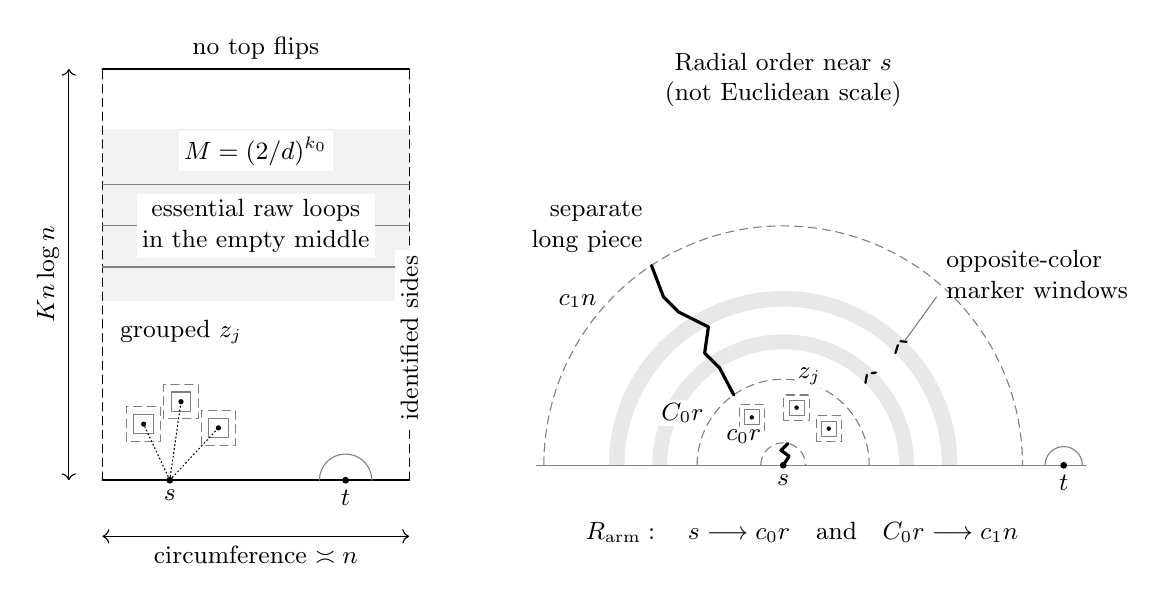
\begin{tikzpicture}[x=.95cm,y=.95cm,font=\small,line cap=round,line join=round]
  \path[fill=gray!10] (0,2.4) rectangle (4.1,4.7);
  \draw[thick] (0,0) -- (4.1,0);
  \draw[thick] (0,5.5) -- (4.1,5.5);
  \draw[densely dashed] (0,0) -- (0,5.5);
  \draw[densely dashed] (4.1,0) -- (4.1,5.5);
  \foreach \y in {2.85,3.4,3.95} {\draw[gray] (0,\y) -- (4.1,\y);}
  \node[fill=white,inner sep=2pt] at (2.05,4.4) {$M=(2/d)^{k_0}$};
  \node[align=center,fill=white,inner sep=2pt] at (2.05,3.4)
    {essential raw loops\\in the empty middle};
  \node[above] at (2.05,5.5) {no top flips};
  \draw[<->] (-.45,0) -- (-.45,5.5);
  \node[rotate=90,above] at (-.45,2.75) {$Kn\log n$};
  \draw[<->] (0,-.75) -- (4.1,-.75);
  \node[below] at (2.05,-.75) {circumference $\asymp n$};
  \fill (.9,0) circle (.045);
  \fill (3.25,0) circle (.045);
  \node[below] at (.9,0) {$s$};
  \node[below] at (3.25,0) {$t$};
  \draw[gray] (2.9,0) arc (180:0:.35);
  \foreach \x/\y in {.55/.75,1.05/1.05,1.55/.7} {
    \draw[gray,densely dashed] (\x-.23,\y-.23) rectangle (\x+.23,\y+.23);
    \draw[gray] (\x-.13,\y-.13) rectangle (\x+.13,\y+.13);
    \fill (\x,\y) circle (.035);
    \draw[densely dotted] (.9,0) -- (\x,\y);
  }
  \node[above] at (1.05,1.7) {grouped $z_j$};
  \node[rotate=90,fill=white,inner sep=2pt] at (4.1,1.9) {identified sides};
  \node[align=center] at (9.1,5.35) {Radial order near $s$\\(not Euclidean scale)};
  \begin{scope}[shift={(9.1,.2)}]
    \foreach \inner/\outer in {1.55/1.75,2.12/2.33} {
      \path[fill=gray!18] (-\outer,0) arc (180:0:\outer)
        -- (\inner,0) arc (0:180:\inner) -- cycle;
    }
    \draw[gray] (-3.3,0) -- (4.05,0);
    \foreach \radius in {.3,1.15,3.2} {
      \draw[gray,densely dashed] (-\radius,0) arc (180:0:\radius);
    }
    \foreach \x/\y in {-.42/.64,.18/.77,.61/.49} {
      \draw[gray,densely dashed] (\x-.17,\y-.17) rectangle (\x+.17,\y+.17);
      \draw[gray] (\x-.1,\y-.1) rectangle (\x+.1,\y+.1);
      \fill (\x,\y) circle (.03);
    }
    \fill (0,0) circle (.045);
    \node[below] at (0,0) {$s$};
    \draw[line width=1.15pt] (0,0) -- (.08,.12) -- (-.03,.2) -- (.06,.29);
    \draw[line width=1.15pt] (-.66,.94) -- (-.85,1.3) -- (-1.05,1.5)
      -- (-1,1.85) -- (-1.4,2.05) -- (-1.6,2.25) -- (-1.76,2.67);
    \draw[densely dashed,thick] (1.1,1.1) -- (1.12,1.22) -- (1.24,1.24);
    \draw[densely dashed,thick] (1.5,1.5) -- (1.55,1.66) -- (1.65,1.65);
    \node[above left,fill=white,inner sep=1pt] at (-.25,.25) {$c_0r$};
    \node[left,fill=white,inner sep=1pt] at (-1.02,.7) {$C_0r$};
    \node[above left,fill=white,inner sep=1pt] at (-2.45,2.06) {$c_1n$};
    \node[above,fill=white,inner sep=1pt] at (.35,1.03) {$z_j$};
    \node[align=left,anchor=west] at (2.05,2.55) {opposite-color\\marker windows};
    \draw[gray] (2.05,2.25) -- (1.63,1.67);
    \node[above left,align=right] at (-1.75,2.72) {separate\\long piece};
    \fill (3.75,0) circle (.045);
    \draw[gray] (3.5,0) arc (180:0:.25);
    \node[below] at (3.75,0) {$t$};
    \node[align=center] at (.25,-.9)
      {$R_{\rm arm}:\quad s\longrightarrow c_0r\quad\text{and}\quad C_0r\longrightarrow c_1n$};
  \end{scope}
\end{tikzpicture}
\caption{The charged cylinder and its two separate arm requirements (schematic, not to scale). The vertical sides in the left panel are identified. Endpoints are grouped at scale $r=n^{1-\varepsilon}$ near $s$, while $t$ is at distance of order $n$; dotted lines are charge strings, not actual paths. The middle observable counts essential raw loops wholly in its strip, not the actual winding cycle used in the later reconstruction event $E$. On the right, the two solid arm pieces need not be connected. The extra opposite-color marker windows lie strictly between radii $2C_0r$ and $c_1n/2$, away from all conditioned cutoff data. Buffers and the finite endpoint configuration are fixed before the mesh limit; omitted distances and radial ratios are not represented metrically.}
\label{fig:charged-cylinder}
\end{figure}


\paragraph{The sign table.}
For a bottom child disk let \(a\in[0,1]\) be the total endpoint
charge in it. Lemma~\ref{physical:winding} gives the following
wrong-expansion numerators, all divided by \(\sin\lambda\):
\begin{equation}\label{physical:charged-table}
 \begin{array}{c|l}
 \text{flips in the child interval}&\text{numerators}\\ \hline
 0&\sin((2-a)\lambda),\quad\sin((1+a)\lambda)\\
 1&\sin(a\lambda)\quad(s),\quad\sin((2-a)\lambda)\quad(t)\\
 2&\sin((3-a)\lambda),\quad\sin(a\lambda).
 \end{array}
\end{equation}
A same-boundary child interval spans less than one period: otherwise
its lift and a period translate cannot be disjoint. Thus each flip
is counted at most once. Top child disks use the zero-flip row.
Contractible wrong-expansion loops have weight
\(2\cos((1-a)\lambda)>0\), and essential loops have weight
\(2\cos(a\lambda)>0\). All entries in the table are nonnegative
except possibly \(\sin((3-a)\lambda)\). In particular, we do not
discard its sign.

Let \(N_j\) count the prescribed local loops at \(z_j\), and
let \(N_t\) count local \(t\)-straddles. Set
\[
 U_\pm=\prod_j u_\pm(a_j)^{N_j},\qquad
 M=(2/d)^{k_0},
\]
where \(k_0\) counts essential closed loops wholly inside an empty
middle strip separated from both ends by enlarged \(O(n)\) bands.
Under either positive cap law, \(M\ge1\) and has polynomial
moments: the strip is covered by \(O(K\log n)\) fixed-ratio
passage bands. Let \(\mathcal T\) be the event of a raw bottom-to-top
through arc. Successive noncontractible actual cycles in separated
transverse bands block such an arc, so Propositions~\ref{prop:routing}
and \ref{prop:screens} give
\begin{equation}\label{physical:through-rarity}
 \PP_\pm(\mathcal T)\le Cn^{-cK}.
\end{equation}
Here \(c>0\) is independent of \(K\). On \(\mathcal T\),
there is no essential closed raw loop and hence \(M=1\).

\paragraph{Local factors and passage errors.}
Let \(Y_\pm\) be the spin integrands relative to their corresponding
positive cap laws. Let \(E\) be the event that the \(s\)-gap
connects actually in its color to a noncontractible cycle near the
bottom, before the middle strip. On \(E\) no child disk cuts off
\(s\), and there is no through arc.  The isolated local factors, relative
to their respective positive cap weights, are
\[
\begin{array}{c|cc}
 \text{local feature}&Y_+&Y_-\\ \hline
 \text{loop around }z_j&u_+(a_j)&u_-(a_j)\\
 s\text{-straddle}&1&0\\
 t\text{-straddle}&1&d\\
 \text{empty-middle essential loop}&2/d&2/d\\
 \text{disk enclosing }s\text{ and all endpoints, not }t&d&1.
\end{array}
\]
The last row covers the intermediate scales between the grouped endpoints
and \(t\); its correct factor is at most one.  The remaining features are
controlled by the passage inventory in the following bounds:
\begin{align}
 |Y_+|&\le M U_+ C^{1+X},\label{physical:correct-majorant}\\
 |Y_-|&\le M U_-d^{N_t}C^{1+X},\label{physical:wrong-majorant}\\
 Y_-&\ge M U_-d^{N_t}C^{-(1+X)}\quad\text{on }E,
 \label{physical:wrong-minorant}
\end{align}
where \(X\) has every fixed exponential moment uniformly in \(n\).
Its passage inventory uses only fixed bottom and top bands,
independently of \(K\), together with the grouped endpoint patch
at scale \(r\).

To prove these bounds, remove locally contained small boundary disks
in descendant order, closing the removed family under descendants.
Their diameters are less than a small fixed fraction of \(n\),
so they contain at most one bottom flip. Lemma~\ref{physical:cap-elimination}
accounts for all neutral cap factors at aggregate passage cost.
In individual cutoff boxes the remaining weights are exactly the
displayed \(u_\pm(a_j)\) loop factors and, at \(t\), the factor
\(d\) for each wrong-expansion local straddle. At \(s\), a local
straddle has wrong weight zero and the correct neutral factor one.

There is one intermediate-scale case which must not be charged once
per scale. A disk enclosing \(s\) and all endpoints but not \(t\)
has correct effective drop \(s-1\), of weight \(d\le1\), and
wrong numerator \(\sin\lambda\), of weight one. These factors
therefore cause no growing error. If inclusion of the endpoint group
disagrees with inclusion of \(s\), the arc crosses a join of length
\(O(r)\) from the gap to that group. A nonlocal such arc gives a
passage across a fixed proportion of the grouped patch or one of its
separated individual patches. The same is true of a nonlocal
contractible loop enclosing endpoints, since it separates them from
the bottom. Cutoff-edge mismatches give the corresponding buffered
patch passages. Genuinely large arcs and essentials outside the
empty middle give passages in the large boundary bands, individually.
Through-arc weights are bounded before cap normalization by a
constant per arc regardless of winding, and each such arc gives a
boundary-band passage.

This is a finite inventory of fixed-shape passage tests at scales
\(r\) and \(n\).  Trim one qualifying portion from each raw arc or loop
in each test.  Distinct raw components have disjoint cut-surface port
incidences, and the fixed number of tests bounds the multiplicity of a
component.  Thus this inventory is bounded by a fixed multiple of the
packing sum of Definition~\ref{angular:passage-packing}, plus a fixed
constant.  Proposition~\ref{prop:passage-moments} supplies all exponential
moments of \(X\). On \(E\), disks
cutting off \(s\) are impossible. The remaining table entries
form a finite strictly positive set, as the charge list is fixed;
the same counting therefore proves the lower bound
\eqref{physical:wrong-minorant}. Notice that \(d^{N_t}\) has been
retained, as is necessary for \(d<1\).

\paragraph{A relative saving for negative terms.}
Off \(\mathcal T\), a nonzero negative integrand requires a
two-flip disk omitting some of the nearby charge: with all charge
included, the first two-flip numerator is \(\sin(2\lambda)>0\).
Let \(B\) denote occurrence of such a disk, and put
\(B_0=B\cap\{Y_-\ne0\}\cap\mathcal T^c\). Its arc intersects a
short join to the endpoint group and travels to distance of order
\(n\). Both colors have actual traversals along its two sides.
Nonzero weight also excludes every pure local \(s\)-straddle below
a sufficiently small multiple of \(r\), forcing a short gap arm.

Choose the constants and buffers of
Corollary~\ref{disk:grouped-cylinder}: the disjoint endpoint annuli lie
between \(c_0r\) and \(C_0r\), and fixed \(0<c_1<c_2\) give an injective
\(s\)-centered half-disk of radius \(c_2n\), separated from the
\(t\)-patch and the middle by positive \(n\)-scale margins.  Its
half-sector between \(c_1n\) and \(c_2n\) has the required fixed ratio
and permitted attachments, counting all bank classes and retaining the
residual-cap condition.  Let \(R_{\rm arm}\)
be the conjunction of an actual gap arm to \(c_0r\) and a separate
same-color traversal from \(C_0r\) to \(c_1n\). The event
\(B_0\) forces these requirements
and also opposite-color traversals in \(J\ge c\log(n/r)-C\)
spaced intermediate marker bands.

Condition on all endpoint-cutoff data, the \(t\)-cutoff data, and
the remote middle-strip states; write this information as
\(\mathcal H\).  Use as the reference in that corollary the fixed flat
cap law and arm cutoff defining \(P(n)\).  The constants above are chosen
so this law agrees with the cylinder graph, odds, and deterministic walls
through \(c_2n\), and its full cutoff lies beyond \(c_1n\) with the
prescribed buffer.  Its reference arm probability is exactly
\(p_{\mathrm{ref}}=e^{P(n)}\); changing to another fixed flat cutoff
would change \(P\) only by \(O(1)\).  That corollary, based on
Lemma~\ref{lem:relative-arm}, gives
\begin{align}
 \PP_-(E\mid\mathcal H)
 &\ge c\,\PP_-(R_{\rm arm}\mid\mathcal H)
 \ge c' p_{\mathrm{ref}}=c'e^P,\label{physical:arm-main}\\
 \PP_-(B_0\mid\mathcal H)
 &\le C(r/n)^\gamma\PP_-(R_{\rm arm}\mid\mathcal H)
 \label{physical:arm-saving}
\end{align}
for a fixed \(\gamma>0\).
For clarity, the first comparison is relative to the two separate
requirements, not an unconditional arm upper bound. Buffered collar
densities compare those requirements under the stated conditioning.
Their supports avoid the conditioned patches. The two measured
blockers can be joined with fixed relative probability through
cleared corridors around the finitely many endpoint boxes at scale
\(r\). Re-search at scale \(n\) then joins this arm to a winding
cycle before the middle, avoiding \(t\). Conversely an ordinary
longer arm forces the two requirements, giving the second lower
bound. In each marker window the conditional same-color scaffold
preserves the required traversal while making a wall-to-wall screen
which prevents the opposing marker traversal. Thus each additional
opposite marker costs a factor at most \(1-c\), relative to the
traversal requirement and with the separated short arm carried along.
Iteration over \(J\) bands proves \eqref{physical:arm-saving}.

\paragraph{Comparison of the two expansions.}
The positive factor \(W=M U_-d^{N_t}\) is measurable with respect
to \(\mathcal H\).  Multiplying the two conditional inequalities by
\(W\) and averaging gives the relative comparison
\begin{equation}\label{physical:weighted-saving}
 \EE_-[W\one_{B_0}]
 \le \frac Cc(r/n)^\gamma\EE_-[W\one_E].
\end{equation}
Thus the negative contribution is compared to the same main event with
its full weight \(d^{N_t}\), even on states where that factor is small.
The bounded cutoff comparisons then give
\begin{equation}\label{physical:main-mass}
 \EE_-[W\one_E]\ge
 c(\EE_-M)e^{P+D_*}\prod_jF_-(a_j;r).
\end{equation}
Before passage errors, \eqref{physical:weighted-saving} makes the bad
contribution smaller than this main mass by the fixed power
\(n^{-\gamma\varepsilon}\).
On the through event, \(M=1\). Its upper bound uses only the fixed
feature bands, whose polynomial moment exponents do not depend on
\(K\). H\"older's inequality and
\eqref{physical:through-rarity} therefore make its absolute
contribution negligible after choosing a sufficiently large fixed
\(K\). The main mass has an inverse-polynomial lower bound whose
exponent does not depend on \(K\), since \(M\ge1\).

Now hold \(K\) and \(\varepsilon\) fixed. The absorption rule
removes the factors \(C^{\pm(1+X)}\) at an arbitrarily small power
cost. Choose that power smaller than the saving in
\eqref{physical:arm-saving}; the negative and through errors remain
negligible. Off these errors the wrong expansion is nonnegative,
and \eqref{physical:wrong-minorant} supplies its positive main part.
For every sufficiently small \(\eta>0\), increasing constants
if necessary, equality of the two tensor expansions consequently
implies
\[
 Z_-^{\rm cap}(\EE_-M)e^{P+D_*}\prod_jF_-(a_j;r)
 \le C_{\eta,\varepsilon,K}n^\eta
 Z_+^{\rm cap}(\EE_+M)\prod_jF_+(a_j;r).
\]
Here the correct upper bound follows from
\eqref{physical:correct-majorant}, the same separated-patch
comparisons, and absorption. All local lower baselines are inverse
polynomials, so the same argument applies to this upper comparison.

Repeat with both wire polarities reversed on the identical cylinder,
using the same strings, cutoffs, drops, and middle observable \(M\).
The two cap laws are interchanged. Their partition and middle-mean
ratios therefore cancel exactly on multiplication. Local costs in
the two designations differ by \(O(1)\). Taking logarithms gives
\[
 P+D_*+\sum_j\log\frac{F_-(a_j;r)}{F_+(a_j;r)}
 \le o(\log n).
\]
Finally \eqref{physical:cutoff-increment} changes \(r\) to \(n\)
at cost \(O(\varepsilon\log n+1)\). Given any final tolerance,
choose \(\varepsilon\) first sufficiently small and then make the
absorption tolerance smaller still. This proves
\eqref{physical:charge-budget}.
\end{proof}

\section{The four-change observable}
\label{sec:observable}

We determine the probability of the two connection alternatives in a
fixed polygon with four alternating boundary designations.  The finite
boundary-tree calculation produces a bounded observable and identifies
its possible boundary values.  Two analytic steps remain: remove a
diagonal correction from those values, and prove that every interior
limit is holomorphic.  Both steps use matched interior and exterior
walls, with positive normalizations that retain the growth of local
loop weights.  The resulting boundary problem has a strictly convex
target and determines the connection probability.

The analytic inputs are the disk and screening estimates of
Section~\ref{sec:disks}, the local tilt bounds of
Section~\ref{sec:angular}, and the physical current and charge estimates
of Section~\ref{sec:physical}.  The output here is the exact
compatible-mesh polygon formula in Theorem~\ref{thm:fixed-polygon}.
Section~\ref{sec:moving} will transfer it to varying and slit domains.

The four-boundary-change FK-Ising construction of Chelkak and Smirnov
\cite[Section~6]{ChelkakSmirnov2012} is an antecedent of this auxiliary
pairing problem.  We give the finite calculation and the below-one
analytic estimates needed for the present parameter range.

\subsection{The four-mark boundary tree}

Fix $0<q<1$, $d=\sqrt q=2\cos\lambda$, and
$\rho=\lambda/\pi\in(1/3,1/2)$.  Let $\Omega$ be a fixed rational
simple orthogonal polygon in tile coordinates.  Choose an integer
$M\ge1$ such that every wall coordinate belongs to $M^{-1}\Z$.
For $n\in M\N$, the sides of $\Omega$ are exact tile lines at mesh
$n^{-1}$; use the full whole-tile graph of this exact polygon.
All mesh limits in this section are restricted to $n\to\infty$ in
$M\N$.  This compatible sequence is the auxiliary polygon experiment
used below.

The distinct ideal marks $p,b,c,d_0$, in counterclockwise order, lie
in side interiors.  For each ideal mark $v$, choose a flat boundary
gap $v_n$ on its side at distance $O(n^{-1})$.  A gap is the visit
of a primal or dual corner between two consecutive boundary ports;
a port is a tile-side midpoint.  For sufficiently large $n$ the
four chosen gaps are distinct and retain their cyclic order.  The
successive boundary intervals $A,B,C,D$, starting at $p_n$, designate
colors $\mathfrak A,\mathfrak B,\mathfrak A,\mathfrak B$, respectively.
Either global designation is allowed, with no restriction on corner
parities.  In finite diagram descriptions we suppress the subscript
$n$ on the four gaps; limiting boundary statements refer to the ideal
marks.

The local caps on an interval pair the intervening ports between
successive visits of its designated color.  At a marked gap, count its
end visit in exactly the adjacent interval whose designation equals
the color of that gap.  The last designated visit before the change
and the first after it are consecutive, so exactly one adjacent port
is left unmatched there.  It is the interface end associated with
the mark, at distance $O(n^{-1})$ from the ideal point.  Leave these
four unmatched ports open.  The
\emph{open-cap law} gives every resulting closed loop weight $d$, besides
the common positive tile coefficients.  Completing the four ports changes
the loop number by at most two, so this law and either deterministic
completion have density ratios bounded above and below by constants
depending only on $d$.  Write $E_{\mathfrak A}$ for an actual path of
color $\mathfrak A$ from $A$ to $C$, and $E_{\mathfrak B}$ for an actual
path of color $\mathfrak B$ from $B$ to $D$.  Such paths use sampled
edges, without jumps through a boundary identification.
The completion factors here are the two-pairing specialization of the
finite FK reweighting in
\cite[Proposition~4.6, equations~(4.17)--(4.19)]{FengPeltolaWu2024FKConnections},
valid at self-dual weights for every $q>0$.

Use the parameters of the finite winding calculation,
\begin{equation}
 \Delta_0=\frac{\pi}{2\lambda}-\frac32,\qquad
 s=\Delta_0+1,\qquad t=-\Delta_0,
 \qquad (H_A,H_B,H_C,H_D)=(s+1,1,s,0).
 \label{obs:bases}
\end{equation}
A port $i$ on $R$ is high if its preceding gap has the designated
color of $R$, and
$h_i=H_R+\Delta_0\one_{\{i\text{ high}\}}$.
Order the ports starting at $p$.  On a second lap decrease every raw
base by one, compensating the lifted inward normal; in particular the
locally forward drop at $p$ is $-s$.  Put
\begin{equation}
 x=e^{-\ii\lambda},\quad y=e^{\ii\lambda},\quad
 P_0=x^{s+1},\quad G_0=1-y^2,\quad A_R=x^{2H_R+\Delta_0}.
 \label{obs:tree-normalization}
\end{equation}
For every real $a$, the notation $x^a$ means $e^{-\ii\lambda a}$.
Thus $x^{2\Delta_0}=-y^3$, $d=y+y^{-1}$, and $P_0G_0\ne0$.

Ignore internal closed loops and cut the disk along all raw arcs with
endpoints on its boundary.  The adjacency graph of the resulting
regions is a tree: inserting a noncrossing arc splits one existing
region into two and adds one edge.  Root it at the unique region
incident to the gap $p_n$.  A vertex has the common color of its
boundary-gap visits, and
adjacent vertices have opposite colors.  A vertex is \emph{wired} if
one of its visits belongs to an interval designating that vertex's
color.  For a point or boundary gap $z$, let $V(z)$ be its region in
this tree; internal closed loops do not enter this definition.  In
finite tree notation a marked subscript $v\in\{p,b,c,d_0\}$ means
the region $V(v_n)$.  Thus, for example, $H_b$ below means $H_{V(b_n)}$.

We evaluate a current on this tree using the spin convention of
Section~\ref{sec:physical}.  Put
\[
 K(\zeta)=\operatorname{diag}(\zeta,\zeta^{-1}),\qquad
 Q=-e^{\ii\lambda},\qquad L_-=|-\rangle\langle+|.
\]
Direct a simple tile-edge path $\mathcal C$ from $p$ to a lattice
vertex $z$.  At a crossed tile side the spin is measured along the
path's left normal; matrix row and column indices belong to the right
and left tiles, respectively.  Choose a continuous tangent lift whose
initial value lies strictly between the positive boundary tangent at $p$ and
that tangent plus $\pi$.  The \emph{current primitive}
$\mathcal J(\mathcal C)$ sums over one marked step: a mark with tangent
lift $\alpha$ carries $e^{\ii\rho\alpha}L_-$, every earlier step carries
$K(Q)$, and every later step carries the identity.  These matrices are
inserted into the ordinary tile tensors.  A pure diagonal string has
$K(Q)$ at every step and no mark.  Paths with a common start use ordered
lanes, whose order is retained under deformation.  The finite
deformation and tree-evaluation identities are proved in
Appendix~\ref{sec:finite-calculus}; the next lemma evaluates this
current for the four-mark profile.

\begin{lemma}[Caps, alternatives, and the path evaluation]
\label{lem:obs-tree}
If $\mathcal I$ is the number of loops closed by local caps, then
\begin{equation}
 \mathcal I=\#\{\text{unwired tree vertices}\}.
 \label{obs:loop-count}
\end{equation}
Exactly one of $E_{\mathfrak A},E_{\mathfrak B}$ occurs.  Completing
around the separately wired intervals $A,C$ adds one loop on
$E_{\mathfrak A}$ and two on $E_{\mathfrak B}$.

For the edge $e$ associated with an arc from $i$ to $j$, $i<j$, define
\begin{equation}
 m_e=h_i-h_j,\qquad
 w_e=\frac{\cos((m_e-\tfrac12)\lambda)}{\sin\lambda},\qquad
 k_e=-\frac{\cos((m_e+\tfrac12)\lambda)}{\sin\lambda},\qquad
 a_e=x^{h_i+h_j}.
 \label{obs:edge-weights}
\end{equation}
Let $\mathcal P(V)$ be the root-to-$V$ path, with its root order.
After dividing by the open-cap weight, define the boundary-arc
diagonal factor $D_V$ and the primitive factor $H_V$ by
\begin{align}
 D_V&=d^{-\mathcal I}
       \prod_{e\in\mathcal P(V)}k_e
       \prod_{e\notin\mathcal P(V)}w_e,\label{obs:D}\\
 H_V&=d^{-\mathcal I}\sum_{e\in\mathcal P(V)}a_e
       \prod_{f\text{ before }e}k_f
       \prod_{\substack{f\text{ not before }e\\f\ne e}}w_f.
       \label{obs:H}
\end{align}
Here $H_{\rm root}=0$; the common primitive marker factor
$c_*=e^{-\ii\lambda}/(2\sin\lambda)$ has been removed.  The primitive
evaluation to a lattice vertex $z$, with this marker factor removed,
is $H_{V(z)}$.  For the full pure $K(Q)$ string to $z$, let $N(z)$
count the internal raw closed loops surrounding $z$.  Its full
open-cap ratio is
\begin{equation}
 D_{V(z)}(-2/d)^{N(z)}.
 \label{obs:full-diagonal}
\end{equation}
Thus $D_V$ contains only the boundary-arc contribution.  If $e=(u,v)$
is directed from parent to child, the common product $D_e^\circ$ with
the factor for $e$ omitted obeys
\begin{equation}
 H_v-H_u=a_eD_e^\circ,\qquad
 D_u=w_eD_e^\circ,\qquad D_v=k_eD_e^\circ.
 \label{obs:recursion}
\end{equation}
\end{lemma}

\begin{proof}
Attach a thin annulus carrying the caps and continue the four open
ports to its outer boundary.  Along each interval, the annulus joins
precisely the visits of its designated color to the outer boundary.
The other intervening gaps are cut off by the caps.  Therefore a raw
region remains accessible from the outer boundary exactly when it is
wired.  An unwired region acquires only the adjacent capped slivers;
it neither merges with another raw region nor becomes accessible.
After attachment there are two noncrossing open strands.  These leave
three regions touching the outer boundary, and each additional closed
loop adds exactly one region not touching that boundary.  This proves
\eqref{obs:loop-count}.

The raw arcs are the perimeters separating the thickened graphs of the
two colors.  Boundary visits of one color in the same raw region are
connected in that graph: trace within its thickening, then retract to
edges.  Internal closed perimeters only enclose components with no
boundary visits, so restoring them cannot split this boundary class.
There are exactly two noncrossing pairings of the four open ports.
They give, respectively, the actual opposite connection of color
$\mathfrak A$ and of color $\mathfrak B$; both cannot occur because
their endpoints alternate.  Against the exterior pairing that wires
$A,C$ separately, the first pairing forms one loop and the second
forms two.  This proves the connection and completion assertions.

Lemma~\ref{lem:calc-tree-evaluation} gives $w_e$ on an unpassed arc,
$k_e$ on a passed arc, and $c_*a_e$ on the marked arc of the primitive.
For the primitive, an internal loop retains weight $d$ unless it is
marked, in which case its contribution is zero; its factors therefore
cancel against the open-cap weight.  For the full diagonal string,
each enclosing internal loop instead contributes the ratio $-2/d$.
Removing those ratios leaves $D_V$, while removing $c_*$ from the
primitive and dividing the local-cap factors by $d^{\mathcal I}$ gives
\eqref{obs:D}--\eqref{obs:H} and \eqref{obs:full-diagonal}.  In the
difference $H_v-H_u$, every
mark before $e$ has the same factors on both paths.  The only new term
is the mark on $e$, proving \eqref{obs:recursion}, including when some
$w_e$ vanishes.
\end{proof}

The finite boundary-tree and four-mark construction follows
\cite{OpenAIConformalLimits2026}; the identities needed here are proved
locally, without importing its probabilistic estimates.

Define the observable and the open-cap connection probability by
\begin{equation}
 h_n(z)=\frac{\EE_{\rm open}H_{V(z)}}{P_0G_0},
 \qquad r_n=\PP_{\rm open}(E_{\mathfrak A}).
 \label{obs:observable}
\end{equation}
The calculation below identifies the candidate target vertices of a
limit with $r_n\to r$, in marked order $(p,b,c,d_0)$:
\[
 0,\qquad r+d(1-r),\qquad r+y(1-r),
 \qquad y(dr+1-r).
\]
The diagonal factor $D_V$ is the obstruction to obtaining the boundary
lines directly from the finite observable.  We first isolate its role
in the exact tree identities.  Shielding and normalized cancellation
will then give the boundary values, while a separate mixed-current
estimate will prove holomorphicity.  No analytic property is used in
the following calculation.

\subsubsection{The marked subtree and its finite algebra}

For an edge $e$, let $L(e)$ count the marks among $b,c,d_0$ in its
child boundary interval.  They form a consecutive subset; their raw
drops are $s,t,s$.  The endpoint high statuses agree for odd $L(e)$
and differ for even $L(e)$.  Substitution in
\eqref{obs:edge-weights}, using
$\Delta_0\lambda=\pi/2-3\lambda/2$, gives
\begin{equation}
 \begin{array}{c|cc}
 L(e)&w_e&k_e\\ \hline
 0&d,\ 1&-1,\ -d\\
 1\ (b\text{ or }d_0)&1&0\\
 1\ (c)&1&-d\\
 2&1,\ d&0,\ 1-d^2\\
 3&0&1
 \end{array}
 \label{obs:table}
\end{equation}
Paired entries list a high first port and a low first port, in that
order.  For example, the even-$L$ raw base drops are $0,1$, and the
odd-$L$ drops are $s,t,s+1$, respectively, which verify every row.

The union of edges with $L(e)>0$ consists of four terminal legs,
possibly of zero length, and at most one middle chain.  The $p$-leg
has $L=3$ and the other three legs have $L=1$.  A middle chain has
$m\ge1$ edges with $L=2$.  It has type $X$ if its descendant marks
are $c,d_0$, so its ports lie on $B,D$; put $\mathfrak C=\mathfrak B$.
It has type $Y$ if its descendant marks are $b,c$, so its ports lie
on $A,C$; put $\mathfrak C=\mathfrak A$.  These are the only two
consecutive two-mark subsets.  The nested-or-disjoint property of
child intervals rules out any further branch.  Number middle nodes
$0,\ldots,m$ away from the $p$-leg, and denote their colors by $c_j$.
Use $m=0$ for a shared branch node.

Every leg or branch vertex of the marked subtree visits intervals of
both designations and
is wired; this remains true when a leg collapses at its mark.  An
internal middle vertex visits only the two $\mathfrak C$-intervals.
The child of an $L=0$ edge is unwired exactly when the first port is
high.  Consequently
\begin{equation}
 \mathcal I=\mathcal I_0+\mathcal I_{\rm mid},\qquad
 \mathcal I_{\rm mid}=\#\{0<j<m:c_j\ne\mathfrak C\},
 \label{obs:count-split}
\end{equation}
where $\mathcal I_0$ counts high-starting $L=0$ edges.  If $m>0$,
both sides of a middle edge visit both $\mathfrak C$-intervals, so
$E_{\mathfrak C}$ occurs.  For $m=0$, the shared node visits all four
intervals and its color is the connected color.  A middle edge has
$w_e=d$ exactly when its child has color $\mathfrak C$.  Alternating
the colors along the chain therefore gives
\begin{equation}
 F:=d^{-\mathcal I_{\rm mid}}\prod_{L(e)=2}w_e
 =\begin{cases}
 d^{\one_{\{c_0\ne\mathfrak C\}}},&m>0,\\
 1,&m=0.
 \end{cases}
 \label{obs:middle-product}
\end{equation}
Indeed the exponent is the number of $\mathfrak C$-children minus
the number of non-$\mathfrak C$ internal nodes; successive opposite
colors cancel, leaving the displayed endpoint contribution.

Every off-path $L=0$ edge cancels its local-cap factor.  An $L=0$
branch lies in a single interval $R$.  With
\begin{equation}
 g_R(\text{designated color})=\tfrac12,\qquad
 g_R(\text{other color})=-\tfrac12,
 \label{obs:g}
\end{equation}
its parent and child satisfy
\begin{equation}
 \frac{k_e}{w_e}
 =-d^{g_R(\operatorname{col}(v))-g_R(\operatorname{col}(u))},
 \qquad a_e=A_R.
 \label{obs:tail}
\end{equation}
Thus the diagonal ratios telescope.  Two successive primitive
increments cancel: their $w$ values alternate $d,1$, their $k$ values
alternate $-1,-d$, and
$A_R(D_u/w_e+D_v/w_f)=0$ for successive edges $e,f$.

\begin{lemma}[Marked values, line invariant, and uniform bound]
\label{lem:obs-marked}
Call a tree \emph{typical} if its four terminal legs have positive
length.  On a typical tree,
\begin{equation}
 D_p=D_b=D_{d_0}=0,\qquad
 \frac{H_b}{P_0G_0}=\one_{E_{\mathfrak A}}+d\one_{E_{\mathfrak B}},
 \qquad
 \frac{H_{d_0}}{P_0G_0}
 =y\bigl(d\one_{E_{\mathfrak A}}+\one_{E_{\mathfrak B}}\bigr).
 \label{obs:marked-values}
\end{equation}
For each interval $R$, the following expression is constant on its
boundary-gap visits:
\begin{equation}
 \Re(H_V/A_R)-c_R(\operatorname{col}(V))D_V,
 \quad
 c_R(\text{designated color})=-\cos\lambda,
 \quad c_R(\text{other color})=\cos(2\lambda).
 \label{obs:line-invariant}
\end{equation}
Define
\begin{equation}
 \Gamma(\mathfrak A)=P_0y^2,\qquad
 \Gamma(\mathfrak B)=-P_0y,\qquad
 H_V^\circ=H_V-\Gamma(\operatorname{col}(V))D_V,
 \qquad T=\one_{E_{\mathfrak A}}+y\one_{E_{\mathfrak B}}.
 \label{obs:corrected}
\end{equation}
On a typical tree, $H_V^\circ=P_0G_0T$ along the $c$-leg and all
its descendant branches.  On gap visits of $B$ its possible values
are $H_b,P_0G_0T$, and on those of $C$ they are $H_{d_0},P_0G_0T$.

There is $C=C(d)<\infty$ such that, for every finite tree and vertex,
including atypical trees,
\begin{equation}
 |H_V|+|D_V|+|H_V^\circ|\le C,
 \qquad |D_V|\le C d^{\ell_c(V)},
 \label{obs:uniform-bound}
\end{equation}
where $\ell_c(V)$ is the number of $c$-leg edges passed before $V$.
\end{lemma}

\begin{proof}
An unpassed $p$-leg edge has $w=0$.  It kills every term unless it
is the marked edge, and so only the last $p$-leg edge can mark.
The first passed $b$- or $d_0$-leg edge has $k=0$ and kills every
later mark.  Put $h=H/P_0$ temporarily.  At node $0$ of a typical
tree the last $p$-leg mark gives
\begin{equation}
 D_0=F,\qquad h_0=
 \begin{cases}F,&c_0=\mathfrak A,\\-y^3F,&c_0=\mathfrak B.
 \end{cases}
 \label{obs:branch-values}
\end{equation}
The first $b$-leg amplitude $a_e/P_0$ is $-y^2$ or $y^{-1}$ as
the parent color is $\mathfrak A$ or $\mathfrak B$; on the $d_0$-leg
these amplitudes are $-y^4$ or $y$.  Since $w=1$, the value beyond
that edge is the parent value plus its amplitude times $D$.

For completeness the entire middle-chain computation is
\begin{equation}
 \begin{array}{c|c|c|c|c}
 \text{type}&c_0&(h_0,D_0)&(h_1,D_1)&(h_j,D_j),\ j\ge2\\ \hline
 X&\mathfrak A&(d,d)&(d+y,1-d^2)&(yG_0,0)\\
 X&\mathfrak B&(-y^3,1)&(yG_0,0)&(yG_0,0)\\
 Y&\mathfrak A&(1,1)&(G_0,0)&(G_0,0)\\
 Y&\mathfrak B&(-dy^3,d)&(-dy^3-y^2,1-d^2)&(G_0,0)
 \end{array}
 \label{obs:chain-evaluation}
\end{equation}
The chain amplitude $a_e/P_0$ is $y$ in type $X$ and $-y^2$ in
type $Y$.  Apply \eqref{obs:recursion} with the alternating middle
entries of \eqref{obs:table} to obtain each column.  Once a zero
$k$ is passed, every subsequent value stays fixed.  At the near
branch, add the $b$ amplitude in type $X$, the $d_0$ amplitude in
type $Y$; at the far branch add the other amplitude.  If $m=1$, use
column $1$ and the opposite parent color there.  The identities
\begin{equation}
 d+(2-d^2)y=yG_0,\qquad
 -dy^3-(2-d^2)y^2=G_0,
 \qquad y^{-1}-y^3=dG_0,\qquad 1-y^4=dyG_0
 \label{obs:far-identities}
\end{equation}
give exactly \eqref{obs:marked-values}.  For a shared node use
$F=1$ in \eqref{obs:branch-values} and add both leg amplitudes;
its color gives the connection event.  This also verifies that case.

To prove the line invariant, traverse the gap visits of $R$.  Write
$r_i=1$ for a high earlier port $i$ and $r_i=-1$ for a low one.
Its before and after colors satisfy
\begin{equation}
 \Re(a_e/A_R)=\cos((m_e-r_i\Delta_0)\lambda)
       =c_{\rm after}k_e-c_{\rm before}w_e.
 \label{obs:early-port}
\end{equation}
For a high port the last expression is
$\cos(2\lambda)k_e+\cos\lambda\,w_e
 =\sin((m_e+\tfrac32)\lambda)$;
for a low port it is
$-\cos\lambda\,k_e-\cos(2\lambda)w_e
 =-\sin((m_e-\tfrac32)\lambda)$.
These are the displayed cosines because
$\Delta_0\lambda=\pi/2-3\lambda/2$.
At the later port $j$, put $r_j=1$ if it is high and $r_j=-1$ if
it is low.  The traversal is reversed, and the same two
product-to-sum identities give
\begin{equation}
 -\Re(a_e/A_R)=-\cos((m_e+r_j\Delta_0)\lambda)
       =c_{\rm after}w_e-c_{\rm before}k_e.
 \label{obs:late-port}
\end{equation}
Multiply by the real number $D_e^\circ$ and use
\eqref{obs:recursion}.  The change in \eqref{obs:line-invariant}
is zero at every port.  This proves the assertion throughout the
interval, also across a polygon corner: its lifted turn was already
included in the definition of the arc weight.

For $R=B,C$, substitution in \eqref{obs:tree-normalization} gives
\begin{equation}
 \Re\bigl(\Gamma(\operatorname{col}(V))/A_R\bigr)
 =c_R(\operatorname{col}(V)),\qquad
 d\Gamma(\text{designated color})+\Gamma(\text{other color})=-A_R.
 \label{obs:gamma-identities}
\end{equation}
Equations~\eqref{obs:recursion} and \eqref{obs:table} now show that
$H^\circ$ is unchanged on $L=0$ edges of $B,C$.  It is also
unchanged on a $c$-leg edge: here $w=1,k=-d$ and its amplitude is
$A_C$ when the parent is $\mathfrak B$, and $A_B$ when the parent
is $\mathfrak A$, so the second identity cancels the increment.

The line directions in normalized coordinates are exactly
\begin{equation}
 \frac{\ii A_R}{P_0G_0}
 =\frac1{2\sin\lambda}
 \begin{cases}1,&R=A,\\-y^{-1},&R=B,\\y^2,&R=C,\\-y,&R=D.
 \end{cases}
 \label{obs:directions}
\end{equation}
Every $c$-leg vertex visits $B$ and $C$.  By the line invariant
and \eqref{obs:gamma-identities}, its corrected value lies on the
two lines anchored at $H_b$ and $H_{d_0}$ with these directions.
They are distinct since $3\lambda-\pi\in(0,\pi/2)$.
Their intersection is $P_0G_0T$: on $E_{\mathfrak A}$ use
$dy-1=y^2$, and on $E_{\mathfrak B}$ use $y-d=-y^{-1}$.
Every descendant $L=0$ branch lies in $B$ or $C$, so it preserves
that value.  For gap visits of $B$, the only remaining nodes are
on a type-$X$ chain; for $C$, they are on a type-$Y$ chain.
In \eqref{obs:chain-evaluation}, subtract
$\Gamma(c_j)D_j/P_0$ and divide by $G_0$.
At node $0$ this is $F$ for color $\mathfrak A$ and $yF$ for
color $\mathfrak B$; at node $1$ and thereafter it is $T$ whenever
it differs from the corresponding marked value.  The leg resets
and the $L=0$ cancellation prove the two-value assertions.

Finally, erase all off-path $L=0$ factors by
\eqref{obs:count-split}.  The normalized full middle product is
$F\in\{1,d\}$, and a passed middle prefix is killed by its second
edge at latest.  Omitting its possible factor $w=d$ costs only
$d^{-1}$.  At most one $p$-leg mark survives, and no mark survives
after a $b$- or $d_0$-leg reset.  On the $c$-leg each passed edge
multiplies $D$ by $-d$ and its primitive increments are bounded by
a fixed multiple of $1,d,d^2,\ldots$.  Their sum is at most a
fixed multiple of $(1-d)^{-1}$.  A root path has at most one
$L=0$ suffix after leaving the marked subtree.  Its diagonal
ratio has absolute value at most $d^{-1}$ by \eqref{obs:tail},
and paired increments cancel, leaving at most one bounded
increment.  These observations prove both bounds in
\eqref{obs:uniform-bound}.  If the $p$-leg collapses, its single
possible marked contribution is simply absent; if another leg
collapses, its chain is empty.  The same estimates therefore hold
without typicality.  No constant here is asserted to be uniform
as $d$ approaches zero or one.
\end{proof}

\subsection{Compactness and boundary shielding}

The finite tree bounds become compactness estimates once actual
circuits and wall crosscuts shield a small neighborhood from remote
boundary arcs.  We use the two colors successively under the permitted
conditional laws of Section~\ref{sec:disks}.

\begin{lemma}[Continuous limits and shielding]
\label{lem:obs-compactness}
The functions $h_n$ are uniformly bounded and asymptotically
equicontinuous on every compact subset of $\Omega$.  Their lattice
parities have the same locally continuous subsequential limits.
The probability of a typical tree tends to one.

At an unmarked boundary point $u$, including a polygon corner,
\begin{equation}
 \lim_{z\to u}\limsup_{n\to\infty}
 \PP_{\rm open}\bigl(V(z)\text{ has no visit on the interval of }u\bigr)=0.
 \label{obs:boundary-shield}
\end{equation}
Here and below the inner limit uses any lattice vertices tending to
the fixed macroscopic interior point $z$.  Near $b$ and $d_0$,
$V(z)$ lies beyond a corresponding terminal-leg edge with
probability tending to one in this order of limits.  Near $p$ an
unpassed $p$-leg edge remains with probability tending to one.
Near $c$, $V(z)$ lies on the $c$-leg or a descendant $L=0$ branch,
and for every fixed integer $m_0\ge1$,
\begin{equation}
 \lim_{z\to c}\limsup_{n\to\infty}
 \PP_{\rm open}\bigl(\ell_c(V(z))<m_0\bigr)=0.
 \label{obs:c-many-edges}
\end{equation}
\end{lemma}

\begin{proof}
We use the actual crossings and buffered routing of
Propositions~\ref{prop:rectangle-rsw}, \ref{prop:sector-actual},
and \ref{prop:routing}, in the screening form of
Proposition~\ref{prop:screens}.  The precise consequence needed is
as follows: in a fixed-ratio bulk annulus there are two nested
actual circuits of opposite colors with conditional probability
at least $\epsilon>0$; in a fixed-ratio wall sector there are two
successive actual crosscuts of opposite colors between its banks
with the same type of lower bound.  The bound is uniform over the
permitted exterior data of Definition~\ref{disk:regular-collars};
in these fixed wall charts every designated bank class, including
a partial interval, is among the bounded named classes.  Use disjoint
buffers for the two colors, and condition successively; no positive association is
used.  The constants may depend on the fixed polygon and $d$.
All estimates obtained under deterministic completion transfer to
the open-cap law by its bounded density ratio.

Two such wall crosscuts force a raw arc joining the banks between
them.  To see this, trace their thickened perimeters.  The gaps
adjacent to the two crosscut ends have opposite colors on each
bank, so there is an odd number of ports between those ends.
The actual paths prevent a raw strand in this intervening strip
from escaping through either crosscut.  If no raw strand joined
the banks, all the ports on either bank would be paired on that
bank, contradicting oddness.  Thus at least one joining raw arc
separates the deeper neighborhood from the outside.  The same
argument applies in the finitely many convex or concave corner
sectors of the polygon.  In the bulk, the nested circuits prevent
a raw boundary arc from passing from the inside to the outside.

Under deterministic caps, for $K$ disjoint scale buffers, conditioning bounds the
probability of no successful screen by $(1-\epsilon)^K$.
More generally the probability of fewer than $m_0$ successful
buffers is at most
\begin{equation}
 \sum_{j=0}^{m_0-1}\binom Kj(1-\epsilon)^{K-j}.
 \label{obs:screen-tail}
\end{equation}
Indeed, for each proposed set of at most $m_0-1$ successes, require
failure on its complement and condition on those disjoint buffers
one at a time.  The sum tends to zero for fixed $m_0$ as $K\to\infty$.
For the open-cap law, multiply these upper bounds by its fixed
density-comparison constant.

If two nearby interior vertices belong to different boundary-tree
regions, a raw boundary arc intersects a short lattice path between
them and continues to the wall.  Surround that path by disjoint
bulk buffers out to a fixed fraction of its distance from the wall.
The preceding bound makes this event uniformly unlikely as their
separation tends to zero.  The bound on $H$ in
\eqref{obs:uniform-bound} then gives equicontinuity of its expectation.
The same argument allows vertices of different lattice parities.
Piecewise interpolation, followed by Arzel\`a--Ascoli on an exhaustion
of interior compact sets, gives the asserted compactness.

At an ordinary boundary point, a successful local wall screen traps
the deeper neighborhood in a disk whose boundary visits belong
only to its interval.  Every raw region there has a visit on that
interval.  Taking arbitrarily many buffers between $|z-u|$ and a
fixed small radius proves \eqref{obs:boundary-shield}.  At a mark,
the forced raw arc has the corresponding one-mark descendant
interval, except at $p$, where its descendant interval contains
$b,c,d_0$ and the local neighborhood is on the root side.  Hence
the asserted edges are passed at $b,c,d_0$ and unpassed at $p$.
Buffers between a mesh-scale neighborhood of each mark and a
fixed radius show that each terminal leg is nonempty with
probability tending to one.  Finally, take buffers between
$|z-c|$ and a fixed radius avoiding the other marks.  Their
successful raw arcs are distinct nested $c$-leg edges, all passed
before reaching $V(z)$.  Equation~\eqref{obs:screen-tail} proves
\eqref{obs:c-many-edges}, with the mesh limit taken first.
\end{proof}

\subsection{Matched walls and positive normalizations}
\label{obs:paired-walls}

The remaining analytic tasks are to make every limit of $h_n$
holomorphic and to remove the diagonal term in the boundary line
invariant.  We use a two-source mixed estimate for the first task
and a separately normalized diagonal cancellation for the second.

We give a common construction for two plane tensors.  The first has a
source primitive on each bank of the wall.  The second has the full
diagonal string from $p$ to $z$ on the interior bank and no exterior
marker.  A complete wall separates the two positive laws, allowing the
first tensor to factor through the observable $h_n$ and the second to
isolate the signed diagonal factor.  Small gaps will permit reflection
and extraction; their effect is compared only after the local positive
weights have been included in the denominator.

Throughout this construction $q$, the polygon, and all marked
points are fixed.  All changes to a plane diagram involve finitely many
tiles at each mesh; Proposition~\ref{prop:plane-limit} supplies the plane
law and identifies its finite spin ratios with the winding expansion.

\subsubsection{Boundary factors and charge routes}

Put $O=\C\setminus\overline\Omega$.  Replace each used wall contraction
by two copies of the same boundary factor $b_i$, evaluated on the spin
relative to the inward normal of its own bank.  Designate the opposite
wire color on the exterior bank.  The high statuses on the two banks
then agree.  The exterior order from $p$ is $D,C,B,A$, and its normal
lift is $\theta_O=\theta_\Omega+\pi$, with total turn $-2\pi$.
Since
\[
 b_i(c)=(2\sin\lambda)^{-1/2}
       \exp\{\ii c(\rho\theta_i/2+\lambda h_i)\},
\]
using the same factor on this bank gives raw bases $H_R-1/2$.
These are statements about the factors themselves, before either
winding expansion is taken.

A directed pure string of charge $a$ contributes
$\exp(\ii\lambda ac)$ at a crossed spin, where $c=1$ is the
left-normal direction.  Write $H^I$ for either of the exterior profiles
\begin{equation}
\begin{array}{c|cccc}
 &D&C&B&A\\ \hline
 H^{\rm src}&s+1&1&s&0\\
 H^{\rm diag}&3/4&1/2&1/4&0
\end{array}
\label{obs:exterior-profiles}
\end{equation}
and put
\begin{equation}
 P_R=H_R^I-H_D^I-(H_R-H_D),\qquad R=D,C,B,A.
 \label{obs:short-strings}
\end{equation}
Run the charge-$P_R$ string forward along a thin exterior strip of
$R$, with ends at its two marks.  Its interior misses the wall.
Sliding it through a complete bank adds $P_R$ to that bank's raw
base.  In the source case these charges, in exterior order, are
$0,-2s,-2(s+t),-2(2s+t)$.

Take two finite lists of numbers $a_j$, each with sum $1$ and
\begin{equation}
 0<a_j<1,\qquad (1+a_j)\lambda<\pi/2.
\label{obs:small-charges}
\end{equation}
Such lists exist by taking sufficiently many equal charges.
Theorem~\ref{thm:charge-budget} applies to each list separately.
The reason for using two lists is visible in the costs that we will
prove below.  Their combined charge cost is at most
$-2(P+D_*)+o(\log n)$, where $P,D_*$ are the local costs of
Section~\ref{sec:physical}.  The diagonal estimate uses the whole
cost, whereas reflection averages its contribution by one half:
\[
 \begin{array}{c|c}
 \text{diagonal cancellation}&3P+D_*-2(P+D_*)=P-D_*\\
 \text{mixed differences}&3P+D_*-(P+D_*)=2P.
 \end{array}
\]
Lemma~\ref{lem:strict-flip} gives
$P-D_*\le-c_2\log n+O(1)$, while the arm bound of
Lemma~\ref{angular:flat-costs} gives $2P\le-2c_1\log n+O(1)$;
both bounds are recorded in \eqref{physical:flip-costs}.
For mixed differences, this saving pays
the losses left after combining the physical extraction powers
$(1+\rho)+(1-\rho)=2$.  The normalized cost calculations appear in
\eqref{obs:residual-cost} and \eqref{obs:reflected-cost}; the construction
must retain the positive local factors needed for those comparisons.

Index their union in increasing order of scale.  From $p$ run strings
of charge $-a_j$ to bulk points $w_j\in O$ at distances
\begin{equation}
 r_j\asymp R_0L^{j-1}
 \label{obs:endpoint-scales}
\end{equation}
from a fixed pole $z_*\in\Omega$.  They follow one simple outward
cut before splitting at their successive scales, and never return
near the polygon.  Extend the cut notionally to infinity and through
$\Omega$ to $z_*$.  Their total charge before splitting is $-2$.
We first choose a sufficiently large fixed $L$; $R_0$ tends to infinity
only after the mesh limit.

For the source tensor the second probe lies in a connected simply
connected exterior strip along $D$ approaching both $p$ and $d_0$.
It stays on the $D$ side of the cut.  Thin strips for the short strings
are separated at the marks by sector curves, so their sliding
homotopies avoid the probe paths.  At a common initial edge use
parallel lanes in the order specifying the matrix product, placing
pure strings on the non-probe side when they separate.  The lanes
cross one smooth raw strand near a port midpoint; joining them near
tile vertices creates no additional strand crossing.  These choices
give tile paths in fixed homotopy classes with continued turn lifts,
also when wall gaps are opened away from the corridors.

For a wall pattern $g$, let $\Xi_g^{\rm src}(z,u)$ contain the two
one-source primitives from the two incidences of $p$ to $z$ and $u$,
the short strings for $H^{\rm src}$, and the distant strings just
specified.  Let $\Xi_g^{\rm diag}(z)$ instead contain the full
interior $K(Q)$ string from $p$ to $z$, no exterior source, and the
short strings for $H^{\rm diag}$ with the same distant strings.
At each cut wall side the ordinary contraction is replaced by the
two boundary factors above.  At a shared edge the ordered lanes
specify the order of matrix composition.  These prescriptions,
together with the ordinary physical tile tensors elsewhere, define
the two finite insertions completely.

\subsubsection{Positive laws and local normalizations}

Complete the designated primal intervals separately on every wall
component.  At fixed mesh and fixed insertion data, first divide each
modified finite partition in a planar approximation by its uncut
finite vacuum partition, including the common tile coefficients.
The symbols $\Xi_g^{\rm src}$, $\Xi_g^{\rm diag}$, and
$Z_g^{\rm cap}$ denote the resulting plane limits of those ratios.
For the spin tensors, Proposition~\ref{prop:plane-limit} identifies
these with the limits of the same fixed finite-insertion ratios
as both torus periods tend to infinity.  No symbol denotes an
absolute infinite partition.
Write $\mu_g$ for the resulting positive deterministic-cap law at
that fixed mesh; $g=f$ denotes the complete wall.  The exact winding
identity on finite planar approximations passes to the plane limit as
\begin{equation}
 \frac{\Xi_g}{Z_g^{\rm cap}}=\EE_{\mu_g}\mathcal O_g,
 \label{obs:diagram-normalization}
\end{equation}
where $\mathcal O_g$ is the oriented diagram sum divided, for each
pairing, by its deterministic-cap loop weight.  Remote unchanged
loops have ratio $1$ after summing orientations, as required for
this passage by Proposition~\ref{prop:plane-limit}.
For a complete wall the positive law factors exactly as
$\mu_f=\mu_{\rm in}\otimes\mu_{\rm ext}$: the two raw pairings and
their separate cap disks have no shared connection.  Here
$\mu_{\rm ext}$ is the positive exterior factor with the stated
deterministic caps, obtained from those finite capped
approximations in the same limit.

We will also use its open-cap version.  Re-pairing its four loose
ports changes only the completed cycles involving the finitely
many boundary-connected components.  Let
$\Delta\ell_{\rm ext}$ be this finite change, open minus
deterministic, and put
\begin{equation}
 R_{\rm ext}=d^{\Delta\ell_{\rm ext}},\qquad
 \dd\mu_{\rm ext,open}
 =\frac{R_{\rm ext}}{\EE_{\mu_{\rm ext}}R_{\rm ext}}\,
       \dd\mu_{\rm ext}.
 \label{obs:exterior-open-law}
\end{equation}
The change is bounded by two in absolute value.  This definition
does not subtract total counts of possibly infinitely many
exterior loops.

In disjoint buffered boxes of radius a fixed small fraction of $r_j$,
let $N_j$ count raw closed loops surrounding $w_j$ and wholly inside
the box.  Set
\begin{equation}
 U=\prod_j u_+(a_j)^{N_j},\qquad
 u_+(a)=\frac{\cos((1+a)\lambda)}{\cos\lambda}>0.
 \label{obs:distant-tilt}
\end{equation}
For the diagonal tensor additionally use
\begin{equation}
 U_z=(2/d)^{N_0(z)},\qquad
 V_{\rm wt}=w(1/4)^{\sum_{\nu=1}^4N_\nu^{\rm ext}},
 \label{obs:diagonal-tilts}
\end{equation}
where $N_0(z)$ uses the interior cutoff of radius
$\dist(z,\partial\Omega)/8$, and $N_\nu^{\rm ext}$ counts local
exterior straddles at the four flat changes in separated cutoff
patches.  All cutoffs have clear buffers.  If a wall interval of length
comparable to $h$ is removed, a tip is one end of a surviving bank ray.
Let $N_{\rm tip}$ count raw arcs between the two banks of that ray,
around the tip and wholly in a small cutoff box of scale $h$.  Put
\begin{equation}
 T_g=\prod_{\rm tips}(\cot\lambda)^{N_{\rm tip}},\qquad T_f=1
 \label{obs:tip-tilt}
\end{equation}
for a complete wall.  A true corner gap removes comparable lengths
on both incident sides; its two tips therefore have disjoint buffered
cutoffs.  Retained gaps retain their factors in $T_f$.

Fix $\sigma(\mathfrak A)=1$ and $\sigma(\mathfrak B)=-1$, and put
$\epsilon_n(z)=\sigma(\operatorname{col}(z))$ for a lattice vertex.
On the complete wall, the closed-loop parity in
Lemma~\ref{lem:calc-tree-evaluation} gives
\begin{equation}
 \epsilon_n(z)(-1)^{N(z)}
   =\sigma(\operatorname{col}(V(z))).
 \label{obs:parity-sign}
\end{equation}
The two normalized tensors are
\begin{align}
 \mathcal H_g(z,u)
 &=\frac{\Xi_g^{\rm src}(z,u)}
 {Z_g^{\rm cap}\EE_{\mu_g}[UT_g]},
 \label{obs:source-normalization}\\
 \mathcal R_g(z)
 &=\frac{\epsilon_n(z)\Xi_g^{\rm diag}(z)}
 {Z_g^{\rm cap}\EE_{\mu_g}[U_zUV_{\rm wt}T_g]}.
 \label{obs:residual-normalization}
\end{align}
Thus on the complete wall $\epsilon_n(z)$ converts the sign of the
full diagonal factor
\eqref{obs:full-diagonal} to the signed tree convention
$\sigma(\operatorname{col}(V(z)))D_{V(z)}$.  It is the same in the
gapped and filled conventions.

Figure~\ref{fig:paired-walls} shows the bank convention and the
local gap geometry used below.
\begin{figure}[tbp]
\centering
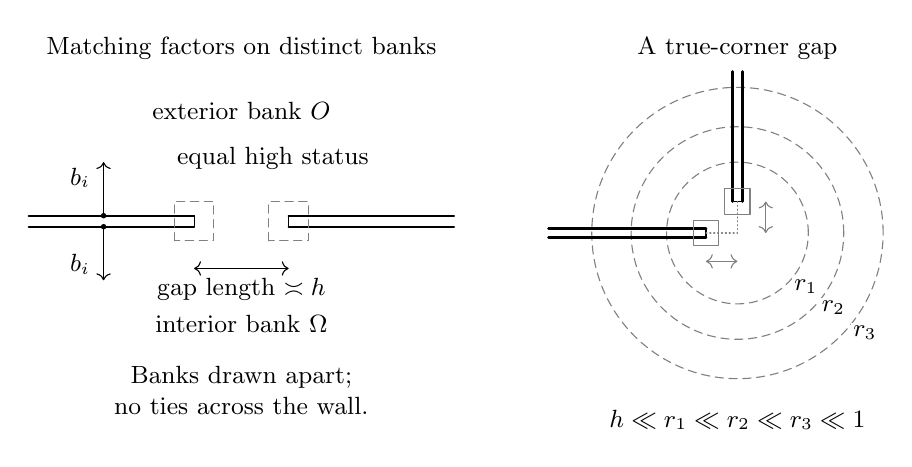
\begin{tikzpicture}[x=1cm,y=1cm,font=\small,line cap=round,line join=round]
  \node[align=center] at (2.7,4.5) {Matching factors on distinct banks};
  \node at (2.7,3.7) {exterior bank $O$};
  \node at (2.7,1.0) {interior bank $\Omega$};
  \foreach \y in {2.23,2.37} {
    \draw[line width=.8pt] (0,\y) -- (2.1,\y);
    \draw[line width=.8pt] (3.3,\y) -- (5.4,\y);
  }
  \draw (2.1,2.23) -- (2.1,2.37);
  \draw (3.3,2.23) -- (3.3,2.37);
  \draw[gray,densely dashed] (1.85,2.05) rectangle (2.35,2.55);
  \draw[gray,densely dashed] (3.05,2.05) rectangle (3.55,2.55);
  \fill (.95,2.37) circle (.035);
  \fill (.95,2.23) circle (.035);
  \draw[->] (.95,2.4) -- (.95,3.05);
  \draw[->] (.95,2.2) -- (.95,1.55);
  \node[left] at (.9,2.85) {$b_i$};
  \node[left] at (.9,1.75) {$b_i$};
  \node at (3.1,3.1) {equal high status};
  \draw[<->] (2.1,1.7) -- (3.3,1.7);
  \node[below] at (2.7,1.7) {gap length $\asymp h$};
  \node[align=center] at (2.7,.15)
    {Banks drawn apart;\\no ties across the wall.};
  \begin{scope}[shift={(9,2.15)}]
    \foreach \radius in {.9,1.35,1.85} {
      \draw[gray,densely dashed] (0,0) circle (\radius);
    }
    \draw[line width=1pt] (-2.4,.06) -- (-.4,.06);
    \draw[line width=1pt] (-2.4,-.06) -- (-.4,-.06);
    \draw[line width=1pt] (-.06,.4) -- (-.06,2.05);
    \draw[line width=1pt] (.06,.4) -- (.06,2.05);
    \draw (-.4,-.06) -- (-.4,.06);
    \draw (-.06,.4) -- (.06,.4);
    \draw[gray,densely dotted] (-.4,0) -- (0,0) -- (0,.4);
    \draw[gray] (-.56,-.16) rectangle (-.24,.16);
    \draw[gray] (-.16,.24) rectangle (.16,.56);
    \node[below right,fill=white,inner sep=1pt] at (.68,-.55) {$r_1$};
    \node[below right,fill=white,inner sep=1pt] at (1.03,-.82) {$r_2$};
    \node[below right,fill=white,inner sep=1pt] at (1.43,-1.14) {$r_3$};
    \draw[<->,gray] (-.4,-.36) -- (0,-.36);
    \draw[<->,gray] (.36,0) -- (.36,.4);
    \node[align=center] at (0,2.35) {A true-corner gap};
    \node[below] at (0,-2.12) {$h\ll r_1\ll r_2\ll r_3\ll1$};
  \end{scope}
\end{tikzpicture}
\caption{Paired walls and the local geometry of gap closure. Each surviving wall has distinct interior and exterior bank incidences, opposite wire designations, and matching factors $b_i$ evaluated with their own normals. Opening a straight gap produces two separately buffered tips; at a true corner, comparable lengths are removed on both incident sides. The dotted corner records where the filled wall would lie and supplies no connection or boundary segment for a Jordan closure. The nested radii satisfy $h\ll r_1\ll r_2\ll r_3\ll1$, with the mesh limit taken before gap closure. All geometry is schematic.}
\label{fig:paired-walls}
\end{figure}


\begin{remark}[Positive normalization and passage errors]
\label{obs:normalization}
For any positive $A$, writing $\nu_A=A\mu/\EE_\mu A$ gives the exact
identity
\[
 \frac{\EE_\mu\mathcal O}{\EE_\mu A}
       =\EE_{\nu_A}(\mathcal O/A).
\]
Consequently an exceptional event is discarded under the tilted law,
using moments of $\mathcal O/A$; its unweighted probability alone
does not control a normalized signed tensor.

We will also use the following elementary quantitative form.  Suppose
$Y_n\ge0$, $\EE Y_n\ge C^{-1}n^{-a}$,
$\EE Y_n^2\le Cn^a$, and $X_n\ge0$ has bounded exponential moments
at every fixed rate.  Then for fixed $K\ge1$ and every $\eta>0$,
\begin{equation}
 C_\eta^{-1}n^{-\eta}
 \le\frac{\EE[Y_nK^{\pm X_n}]}{\EE Y_n}
 \le C_\eta n^\eta.
 \label{obs:absorb-passages}
\end{equation}
Indeed, split at $X_n=\delta\log n$, with
$\delta\log K<\eta$.  On this event the extra factor has the desired
bounds.  Cauchy--Schwarz and an exponential moment of sufficiently
large fixed rate make both tail expectations, with or without
$K^{X_n}$, smaller than any prescribed inverse power of $n$.
Choose that power larger than $a+1$ and divide by $\EE Y_n$.
Increasing $C_\eta$ covers bounded $n$.  The positive local factors
used below have the required polynomial bounds by
Proposition~\ref{prop:tilts}; this is the precise meaning of an
$o(\log n)$ passage allowance.
\end{remark}

\begin{lemma}[Separated surface partitions]
\label{lem:obs-surface}
Let finitely many straight finite wall fragments have fixed shapes
and positive mutual separation.  Complete each as an isolated
positive slit, with boundedly many wire changes.  If $Z_s$ is its
partition relative to the plane vacuum and $Z_{\rm all}$ is the
partition with all these slits, then
\begin{equation}
 Z_{\rm all}\asymp\prod_s Z_s,
 \label{obs:surface-product}
\end{equation}
uniformly in the mesh.  Reversing all cap-wire polarities on both
banks of one straight slit changes $Z_s$ by a bounded factor.
The same holds under a lattice symmetry with cap data transported
and color names exchanged when necessary.

Positive local nest or straddle factors in separated buffered patches
can also be compared in products under these completed-slit laws.
In particular, the baseline tip and flat-change expectations in a
correct expansion and in its reflected complementary convention
are comparable when their local counts and weights are transported
by that reflection.  Constants may depend on the fixed slit geometry
and the chosen positive weights.
\end{lemma}

\begin{proof}
Enclose each fragment in its own patch, with a vacant bulk collar
and a further disjoint buffer.  Let $X_s$ count passages through that
collar.  Compare the actual incremental loop change $\Delta\ell_s$
of the surgery with $\Delta\ell_s^\circ$, calculated after closing
the patch ports by the same arbitrary pairing before and after
surgery.  A strand end whose continuation is not determined inside
the patch must first traverse the collar.  There are $O(X_s)$ such
ends; changing their pairing changes either completed cycle count
by at most their number.  Therefore
\[
 |\Delta\ell_s-\Delta\ell_s^\circ|\le C X_s,
\]
including when other surgeries have already been performed outside.
For a fixed sufficiently large $K$, simultaneous truncation
$X_s\le K$ has probability bounded below under the law with all
completed slits, by Proposition~\ref{prop:passage-moments}.
On that event all actual surgery weights and their local versions
are comparable.  With
$G_s=d^{\Delta\ell_s^\circ}\one_{\{X_s\le K\}}$, it follows that
\[
 Z_{\rm all}\asymp\EE_0\prod_sG_s,
 \qquad Z_s\asymp\EE_0G_s.
\]
The bounded collar comparison of Lemma~\ref{disk:initial-collars},
applied successively across the disjoint collars to these nonnegative
local functions, compares the first expectation with the product
of the others.  This proves \eqref{obs:surface-product}.

Translate an isolated straight fragment by one tile step tangent
to itself.  Plane invariance, with color exchange if required,
preserves its partition.  The translated caps agree with the
reversed caps except at a bounded number of ports near tips and
changes.  The remaining pairings differ on only that many ends,
so their completed loop counts differ by a bounded number.  Since
$d>0$ is fixed, the ratio of partitions is bounded above and below.
The same argument after a lattice symmetry proves its stated form.
This compares partitions, and makes no pointwise density assertion
for changing every cap along a long wall.

Finally condition successively outside the separated local buffers.
The bounded collar densities of Lemmas~\ref{disk:initial-collars}
and~\ref{disk:thin-collars} compare the expectations of arbitrary
nonnegative functions supported on their smaller patches, so they
apply to the positive powers of the indicated counts.  Reflection
across a ray exchanges its two banks and wires; reflection at a flat
change exchanges its two assignments.  Local factors on opposite
banks use disjoint half-sector buffers up to the intact wall and
are compared separately.  These charts contain only the fixed
adjacent bank portions, so all their named classes, including
partial intervals, have a fixed bound.  Reducing a cutoff by a fixed
factor when needed costs a bounded ratio by Proposition~\ref{prop:tilts}.
This proves the last assertion without identifying the two global
cap laws pointwise.
\end{proof}

\subsubsection{Inversion and the exterior phase}
On a complete wall, slide the short strings onto their bank.  The
resulting raw profile is
\[
 H_R-\tfrac12+P_R=H_R^I+H_D-\tfrac12-H_D^I,
\]
so it differs from the ideal profile by one constant.  A constant
shift cancels on an unmarked arc; with one outward source it produces
one fixed phase.  Use inversion $\iota(\zeta)=1/(\zeta-z_*)$ and a
continuous lift
$\psi=\arg\iota'$ off the chosen cut.  The inverted normal is
$\theta_O+\psi$.  On the clockwise exterior lap $\psi$ increases by
$4\pi$, making its total normal turn $2\pi$.  For an oriented
drawn arc with signed cut-intersection number $I$, its image turn is
\begin{equation}
 W^I=W+\psi(\mathrm{end})-\psi(\mathrm{start})-4\pi I.
 \label{obs:inversion-turn}
\end{equation}
The boundary normal factors cancel the endpoint terms.  At a marked
arc the two pieces have additional start terms, canceled by the
change of the source tangent gauge $e^{\ii\rho\alpha}$.
Prefix intersections are unchanged topologically.  The total
charge $-2$ along the unsplit cut supplies exactly the remaining
multiplier from $-4\pi I$ in the winding phase.  This proves that
every bounded open arc before the first splitting scale has its
ideal inverted-disk weight, up to the common source phase.  Only
turn lifts and intersections were used; the exterior probability
law has not been transformed by conformal invariance.

For the source profile, let $H^I_{V^I(u)}$ be the $c_*$-removed
tree polynomial \eqref{obs:H} for the ideal four-change profile in
the inverted coordinates on $O\cup\{\infty\}$.  Its tree is formed
from the physically sampled exterior boundary arcs, and its root
is the exterior gap at $p$.  Define
\begin{equation}
 J_n(u)=
 \frac{\EE_{\mu_{\rm ext,open}}H^I_{V^I(u)}}{P_0G_0}.
 \label{obs:exterior-observable}
\end{equation}
The law here is exactly \eqref{obs:exterior-open-law}; it has not
been conformally transformed.  The common inversion phase is not
part of $J_n$.  Its raw boundary arcs form a finite tree almost
surely by Proposition~\ref{prop:plane-limit}; no tiles at infinity
are needed.  The same finite tree bounds as in the interior and
Propositions~\ref{prop:passage-moments} and~\ref{prop:screens}
give local boundedness and equicontinuity in the reserved strip.
Indeed a nonlocal arc has a fixed-scale passage near the bounded
wall, whereas separating two nearby probe points requires an arm
from their vicinity to that wall.  At $p$ and $d_0$, local two-color
screens give the corresponding tree boundary values: the value at
$p$ tends to zero, while at the second exterior mark $d_0$ the
normalized value differs by $o(1)$ in the same ordered limit from
the expectation of
$\one_{E^I}+d\one_{(E^I)^c}$, where $E^I$ is the first exterior
designation's opposite-interval connection.  That expectation lies
in $[d,1]$.
Thus every locally uniform limit $J$ is continuous and
nonconstant on this connected strip.

For the unmarked profile the ideal open-arc weights are strictly
positive.  One and three changes give $w(1/4)=w(3/4)$; two changes
give $\sin(3\lambda/2)/\sin\lambda$; zero or all four give the
ordinary staggered cap weights.  The local drop is $1/4$ also at
$p$: the physical exterior base increases by $1$ on a second lap,
and the launches of total charge $-2$ supply the missing shift.
The wrong local drop is $-1/4$.  These shifts are unchanged by
gaps away from the marks.  Cap elimination, first inside the four
cutoffs and then at a fixed small wall scale, therefore gives for
the ideal arc product $A^I$, divided by deterministic cap loops,
\begin{equation}
 C^{-(1+X_0)}\le A^I/V_{\rm wt}\le C^{1+X_0},
 \label{obs:ideal-positive}
\end{equation}
where $X_0$ has bounded exponential moments at every fixed rate,
also under the displayed local tilts.  In particular its normalized
positive expectation is bounded above and below.

\begin{lemma}[Distant signed normalization]
\label{lem:obs-distant}
For a closed exterior raw loop $\gamma$, let
$A_\gamma=\sum_{w_j\text{ inside }\gamma}a_j$, where inside is
its physically bounded side, and set
\begin{equation}
 y_\gamma=
 \begin{cases}
 \cos((A_\gamma-1)\lambda)/\cos\lambda,
       &\gamma\text{ surrounds the wall},\\
 \cos((1+A_\gamma)\lambda)/\cos\lambda,
       &\gamma\text{ does not surround the wall}.
 \end{cases}
 \qquad Y=\prod_\gamma y_\gamma.
 \label{obs:closed-loop-ratios}
\end{equation}
These are exactly the changed closed-loop ratios in either exterior
construction.  For sufficiently large fixed $L$, under the positive
exterior law $\nu\propto U\mu_{\rm ext}$, or
$\nu\propto UV_{\rm wt}\mu_{\rm ext}$, one has
\begin{equation}
 \EE_\nu(Y/U)\ge c_L>0,
 \qquad \EE_\nu|Y/U|^p\le C_{p,L}\quad(p>0).
 \label{obs:distant-bounds}
\end{equation}
The bounds are uniform in large $R_0$ and fine mesh, and hold with
the same type of constants after conditioning in separated
near-wall patches away from the endpoint buffers.
\end{lemma}

\begin{proof}
Sum the two loop orientations and count counterclockwise string
intersections.  If the loop surrounds the wall, it surrounds all
launches and its charge contribution is $2-A_\gamma$; otherwise
it surrounds only the indicated endpoints.  This gives
\eqref{obs:closed-loop-ratios}.  A closed loop cannot separate the
marker of a nonzero source term from the connected wall: that
marker lies on an open arc to the wall.  Consequently source
prefixes make no additional closed-loop ratios, even when open
arcs go far.  Loops surrounding the wall with endpoint mass $0$
or $2$ have ratio $1$, and loops surrounding no insertion are
unchanged.  Only finitely many ratios are nontrivial at each mesh.

Choose a fixed large geometric constant $K$.  In corridor $j$,
between radii $Kr_j$ and $r_{j+1}/K$, every winding loop encloses
exactly the first $j$ endpoints.  Write $M_j$ for its product of
ratios, and $M=\prod_jM_j$.  For $0\le A\le2$,
\[
 1\le v(A):=\frac{\cos((A-1)\lambda)}{\cos\lambda}
       \le(\cos\lambda)^{-1},
\]
so every $M_j\ge1$.  Besides the local nests in $U$ and these
corridor loops, every nontrivial loop has a passage in one of
finitely many fixed-ratio endpoint bands.  A loop excluding $z_*$
and enclosing an endpoint outside its cutoff separates that
endpoint from $z_*$ and has such a passage.  A winding loop with
an intermediate endpoint mass either lies in its corridor or
meets a bounding band.  Fixed box and shell covers, with the
tilt-edge bounds of Proposition~\ref{prop:tilts}, therefore give
a count $X$ such that, for each fixed $t$,
\begin{equation}
 \EE_\nu e^{tX}\le C_t,
 \qquad |Y/U|\le MC^X,
 \qquad Y/U\ge MC^{-X}\ \text{on }\mathcal B^c.
 \label{obs:distant-sandwich}
\end{equation}
Here $\mathcal B$ is the event that a loop excluding $z_*$ encloses
at least two endpoints.  Off this event all nonlocal ratios other
than the corridor factors belong to a fixed finite positive set:
an excluded-wall loop contains at most one small charge, to which
\eqref{obs:small-charges} applies.  The constants in the exponential
bound are independent of $R_0$ and sufficiently large $L$.

Every winding loop in a corridor traverses one of $O(\log L)$
dyadic passage bands.  Color their disjoint buffers with a fixed
number of colors, apply the conditional passage moment bound in
one color successively, and use H\"older across colors.  Their
supports avoid the endpoint tilts.  Thus, for each fixed $b>0$,
\begin{equation}
 \EE_\nu M^b\le C_bL^{A_b}.
 \label{obs:corridor-moments}
\end{equation}

If a bad loop has smallest enclosed endpoint index $j$, it crosses
corridor $j$ radially.  It cannot cross any raw winding loop there,
so $M_j=1$ on this event, denoted $\mathcal B_j$.  Successive actual
circuit screens in that corridor, conditioned on all endpoint
patches and the other corridors, give
\[
 \PP_\nu(\mathcal B_j\mid\mathcal G_j)\le CL^{-\alpha},
\]
where $\mathcal G_j$ includes the variables $M_i$, $i\ne j$.
This uses only the conditional screen bounds of
Proposition~\ref{prop:screens}; the held data impose permitted
radial cap partitions on the fresh annuli, which have no bank hubs.
With $m=\EE_\nu M\ge1$ and
$M^{(j)}=\prod_{i\ne j}M_i$, we obtain the relative estimate
\begin{equation}
 \EE_\nu[M\one_{\mathcal B}]
 \le\sum_j\EE_\nu[M^{(j)}
            \PP_\nu(\mathcal B_j\mid\mathcal G_j)]
 \le C L^{-\alpha}m.
 \label{obs:bad-before-passages}
\end{equation}

For completeness, the passage factor preserves a strict relative
power.  Set $c=\log C$ and choose $\vartheta>0$ with
$c\vartheta<\alpha/2$.  Splitting at $X=\vartheta\log L$ gives
\[
 \EE_\nu[MC^X\one_{\mathcal B}]
 \le C L^{-\alpha+c\vartheta}m
   +(\EE_\nu M^2)^{1/2}
     (\EE_\nu[e^{2cX};X>\vartheta\log L])^{1/2}.
\]
For $t>2c$ the last term is at most
$C_tL^{A_2/2-(t-2c)\vartheta/2}$.  Choose the fixed rate $t$
so large that this exponent is below $-\alpha/2$, and use $m\ge1$.
It follows that
\begin{equation}
 \EE_\nu[MC^X\one_{\mathcal B}]
       \le C'L^{-\alpha/2}m.
 \label{obs:relative-signed-error}
\end{equation}
Likewise, for every $\eta>0$, split at
$X=(\eta/c)\log L+H$ if $c>0$.  Cauchy--Schwarz,
\eqref{obs:corridor-moments}, and an exponential moment with rate
$t>cA_2/\eta$ make the $M$-weighted tail at most $m/2$, by taking
the fixed $H$ large.  Hence
\begin{equation}
 \EE_\nu[MC^{-X}]\ge c_\eta L^{-\eta}m.
 \label{obs:positive-relative-mass}
\end{equation}
For $C=1$ these conclusions are immediate.  Equations
\eqref{obs:distant-sandwich}, \eqref{obs:relative-signed-error}
and \eqref{obs:positive-relative-mass}, with $\eta<\alpha/2$,
give
\[
 \EE_\nu(Y/U)
 \ge\bigl(c_\eta L^{-\eta}-2C'L^{-\alpha/2}\bigr)m>0
\]
once $L$ is sufficiently large.  This proves the uniform positive
lower bound.  All fixed absolute moments follow from
$|Y/U|\le MC^X$, \eqref{obs:corridor-moments}, and H\"older.
The arguments used conditional passage and screen estimates in
buffers separated from the near-wall patches, so the claimed
conditional uniformity follows as well.
\end{proof}

\subsubsection{Source bounds and complete-wall factorization}
We record an absolute bound which will also be needed on exceptional
gapped configurations.  Write each pure string starting at $p$ as a
short connector along the exterior bank toward its non-probe side,
followed by the rest of the string.  Retain the connector's diagonal
matrices in the bank factors, in the original lane order.  Deform only
the remaining path, with its endpoints fixed, by
Lemma~\ref{lem:current-identity}.  This expresses a small displacement
of the continuing route while retaining every crossed-port phase and
the charge at its original endpoint $p$.
Each source can now be put in a regular simple tube with $p$ in
the relative interior of a flat entrance, clear on both sides,
and the target deep inside.  Other tube sides avoid walls,
strings, and the other tube.  Finitely many such choices cover
compact probe sets.

For a fixed pairing minimize crossings of the disjoint raw crosscuts
separating the entrance from the target.  A small separating crosscut
near the entrance cuts off $p$, since it cannot contain the deep
target.  The solid entrance makes it an entire local launch arch,
not a short return of a larger strand.  All other relevant open
crosscuts have macroscopic tube subpassages; repeated visits of one
strand give disjoint such passages.  A tiny separator at the deep
target is a closed loop and cannot carry a nonzero outward source
marker.  The two outward markers cannot lie on one raw arc or on a
closed loop, since its orientation cannot supply two outward ends.

After including the short and distant charges, the local unpassed
drop at either launch is $-s$.  It has weight zero.  Passing its
source prefix changes it to $-s-1$, with the $Q^{-1}$ sign, giving
unit absolute weight.  Thus only the last nested launch arch can
be marked in a nonzero term.  The other local changes $s,t,s$ have
unit weights.  Ordinary small disks cancel their caps by the
finite elimination in Lemma~\ref{physical:cap-elimination}; a
geometric corner without a wire change has zero-drop staggering.
Every remaining choice costs at most a constant per macroscopic
passage.  Thus for a complete wall the absolute source sum divided
by its deterministic loops and by $U$ is bounded by
\begin{equation}
 |Y/U|C^{1+X_0},
 \label{obs:absolute-source-bound}
\end{equation}
with all fixed exponential moments for $X_0$ under the relevant
tilts.  The analogous diagonal bound has the factors $U_z$ and
$V_{\rm wt}$ removed.  Near $z$ the full diagonal changes the loop
weight to $-2$, whose absolute ratio is $2/d$; beyond its cutoff
every enclosing loop has a fixed-scale passage.  Its local
interior changes have unit magnitude, including the exiting
prefix at $p$.  The exterior local changes are exactly the
$V_{\rm wt}$ factors.  These observations prove all fixed
absolute moment bounds for both normalized integrands.

The next factorization keeps the wall complete.  Independence of the
interior and exterior positive laws is exact; the source error comes
from sending the exterior string-splitting scales to infinity.
After this reduction we will compare gapped walls with the complete
wall using the same positive normalizations.

\begin{proposition}[Complete-wall factorization]
\label{prop:obs-factorization}
For the source tensor there are numbers $a_n(R_0,L)$ independent
of both probes, with $c_L\le|a_n|\le C_L$, such that
\begin{equation}
 \begin{aligned}
 \mathcal H_f(z,u)&=a_n(R_0,L)h_n(z)J_n(u)+e_n(z,u;R_0,L),\\
 \lim_{R_0\to\infty}\limsup_{n\to\infty}
       \sup_{(z,u)\in K}|e_n|&=0
 \end{aligned}
 \label{obs:source-factorization}
\end{equation}
for each compact probe set $K$, with sufficiently large fixed $L$.
Every locally uniform subsequential limit of $J_n$ on the reserved
strip is continuous and nonconstant.

For the diagonal tensor, write $\mu_{\rm in}$ for the interior
deterministic-cap law, $R_*=d^{\ell_{\rm open}-\ell_{\rm det}}$,
and $N(z)$ for all closed interior raw loops surrounding $z$.
There is a probe-independent exterior scalar $a_n^I(R_0,L)$ such
that the exact full-wall identity is
\begin{equation}
 \mathcal R_f(z)=a_n^I(R_0,L)
 \frac{\EE_{\mu_{\rm in}}
   [R_*\sigma(\operatorname{col}(V(z)))D_{V(z)}(2/d)^{N(z)}]}
 {\EE_{\mu_{\rm in}}U_z}.
 \label{obs:diagonal-factorization}
\end{equation}
For sufficiently large fixed $L$,
\begin{equation}
 \liminf_{R_0\to\infty}\liminf_{n\to\infty}|a_n^I|>0,
 \qquad \limsup_{R_0\to\infty}\limsup_{n\to\infty}|a_n^I|<\infty.
 \label{obs:diagonal-exterior-nonzero}
\end{equation}
No convergence of either scalar is required.
\end{proposition}

\begin{proof}
On a complete wall the two positive capped laws are independent:
their raw pairings and separate cap disks share no connection.
For the source tensor the interior factor is $h_n$ times
$c_*P_0G_0$ and the open-to-deterministic partition ratio.  That
ratio is bounded above and below, because only the four unmatched
ports are re-paired.  The diagonal finite tree expansion gives the
interior factor in \eqref{obs:diagonal-factorization}, with the
parity factor already fixed in \eqref{obs:residual-normalization}.
This proves the exact assertion once $a_n^I$ is defined as the
normalized exterior expectation.

Actual circuits between the bounded wall and the first endpoint
scale make the probability of a boundary raw arc reaching that
scale tend to zero, also under $U$ and $UV_{\rm wt}$ tilts.
On its complement the inversion calculation is exact.  The
moment bounds in Lemma~\ref{lem:obs-distant},
\eqref{obs:ideal-positive}, and
\eqref{obs:absolute-source-bound} make the exceptional contribution
$o(1)$ by H\"older, in the stated order of limits.

Choose $1\ll R_1\ll R_2\ll R_0$ with all successive ratios
diverging.  Truncate the ideal arc factor to zero unless all its
boundary arcs stay inside $R_1$.  It is then readable inside that
radius.  Similarly $Y/U$ is readable outside $R_2$ except when a
raw path joins that radius to an endpoint band: loops created
entirely at the smaller scales have ratio $1$.  Screening makes
both exceptions rare, and the same moments control the product
errors.  The inward relative bulk comparison in
Proposition~\ref{prop:relative-collars} factors the expectations
of the two truncated factors with error $o(1)$.  These collars are
vacant full annuli with no named bank hubs.  To see that it
applies to a signed factor, apply the uniform relative density
bound to its positive and negative real and imaginary parts;
their absolute expectations are bounded by the moment estimates.
The same comparison applied to absolute parts removes the remote
tilt from the near factor.  With $V_{\rm wt}$ present it retains
exactly that near-wall tilt and removes only $U$.

In the source case the near expectation is the normalized ideal
tree observable $J_n$, times its fixed nonzero tree and cap
normalizers.  The far expectation is $\EE_\nu(Y/U)$, bounded
above and away from zero by Lemma~\ref{lem:obs-distant}.
Absorb these constants and the common inversion phase into
$a_n$.  This proves \eqref{obs:source-factorization} and its
uniformity; the assertion about $J_n$ was proved above.
In the unmarked case the near expectation is positive and
bounded above and below by \eqref{obs:ideal-positive}.  Its
product with the positive distant expectation gives
\eqref{obs:diagonal-exterior-nonzero}, including the harmless
common phase.  At no stage is a lower bound for a signed interior
observable used.
\end{proof}

\subsection{Closing wall gaps after positive normalization}
\label{obs:closing-gaps}

\begin{proposition}[Common gap closure]
\label{prop:obs-gap-closure}
Fix the distant strings, their locations, and all other geometric
features.  Open finitely many separated gaps of lengths comparable
to $h$, away from marks and insertion corridors; at a true corner
remove comparable intervals on both sides.  Let $g$ be this wall
and let $f$ fill these gaps, possibly retaining other fixed gaps.
For the tips being filled, take cutoff radii at one fixed positive
fraction of $h$, with buffers clear of the other features for all
small $h$.  Keep the endpoint factor $U$ and all retained cutoff
patches fixed during this closure.  Constants below may depend on
that fixed cutoff fraction.
For the source normalization there are positive numbers $b_n$
independent of $z,u$, with $c\le b_n\le C$, such that
\begin{equation}
 \mathcal H_g(z,u)=b_n\mathcal H_f(z,u)+e_{n,h}(z,u),
 \qquad
 \lim_{h\downarrow0}\limsup_{n\to\infty}
       \sup_{(z,u)\in K}|e_{n,h}|=0.
 \label{obs:source-gap-closure}
\end{equation}
For every fixed interior $z$, the same assertion holds for
$\mathcal R_g(z)$ and $\mathcal R_f(z)$, with a positive bounded
factor $b_n(z)$.  Constants may depend on the fixed remaining
features and on $K$ or $z$.  In particular, a smaller second
collection of gaps can be closed before the first.
\end{proposition}

\begin{proof}
We use the same tile pairings in both cut conventions.  A raw arc
or port interaction is affected if it uses a newly missing port;
the gapped diagram joins the filled raw paths which end there.
For the source case set $S=UT_f$, and for the diagonal case set
$S=U_zUV_{\rm wt}T_f$.  Put $T=T_g/T_f$ and
\begin{equation}
 \nu_g=\frac{ST\mu_g}{\EE_{\mu_g}(ST)},\qquad
 \nu_f=\frac{S\mu_f}{\EE_{\mu_f}S}.
 \label{obs:gap-tilted-laws}
\end{equation}
All factors of $S$ are supported away from the gaps being filled.
Our goal is to separate the normalized diagram into a positive local
multiplier near the gaps and a common signed factor away from them.
The separation is exact on a screening event.  Uniform moments under
both tilted laws will control its complement before the relative
collar comparison factors the two expectations.

\paragraph{The local positive multiplier.}
Choose $h\ll r_1\ll1$.  In the common collars impose an actual
primal screen between the wall rays in the sector carrying primal
wire portions, and an actual dual screen in the other sector,
which has no bank or hub attachment.  The only bank attachments in
the first sector are the two continuous primal ray portions, each
crossing the collar and met by its primal screen.  The sectors have
no direct contact inside the collar.  By testing many separated
shells outside the tip supports, Proposition~\ref{prop:screens}
and the tilt bounds make this event, called $G_{\rm in}$, have
probability tending to one under $\nu_g$, uniformly given remote
data and deeper tip data.  It confines every affected path to the
$r_1$ patches.  The induced outer primal ties are the same in the
two conventions: any connection through a deeper patch enters
the already connected primal screen, also if it bypasses through
one of the wire portions joined by that screen.  Represent those
wires by deterministic connections along the designated intervals.
Euler's formula then makes $\ell_f-\ell_g$ a difference of local
component counts plus deterministic constants.  This conclusion
may first be read with all exterior edges fixed.

There is therefore a local factor $B$ such that, on $G_{\rm in}$,
\begin{equation}
 \mathcal O_g=B\mathcal O_f.
 \label{obs:gap-local-equality}
\end{equation}
This is an identity of the summed diagram expressions, including
when their common exterior factor vanishes: $B$ is formed from
the affected local spin weights and $d^{\ell_f-\ell_g}$, not by
dividing a possibly zero observable.  It is strictly positive.
Indeed the patch is a disk with two radial notches ending at its
separated tips.  A same-bank simple arc, including one threading
the gap, has opposite high statuses at its ends and the ordinary
staggered $d,1$ weights.  For an opposite-bank arc oriented from
the interior port $i$ to the exterior port $j$, high statuses
agree and the endpoint directions are the two interior normals.
The matching factors and the winding formula of
Lemma~\ref{physical:winding} give its orientation sum as
\begin{equation}
 \frac{\cos\{\rho(W+\theta_i-\theta_j)/2\}}{\sin\lambda}.
 \label{obs:opposite-bank-amplitude}
\end{equation}
The lifted turn $W+\theta_i-\theta_j$ is $\pm2\pi$ around one
ray tip, and $0$ across the slot between the two rays.  Thus the
two weights are respectively $\cot\lambda$ and $1/\sin\lambda$,
both positive.  To verify the lift, round the boundary-attached
notches and separate their bank incidences.  The resulting region
is a topological disk, and an affected raw arc is a proper embedded
crosscut: an intermediate bank contact would terminate that raw
arc, while confinement keeps it off the outer patch boundary.
Crosscuts with the same endpoint incidences are ambient-isotopic
relative to this disk boundary.  The isotopy can be fixed in short
endpoint collars, so the endpoint tangents and normal lifts stay
fixed and the integer turn defect cannot change.  For collinear
rays, a representative around a single ray tip has defect
$\pm2\pi$, and a representative across the slot between different
rays has defect $0$.  Any Jordan closure used here follows the
rounded disk boundary, not the virtual filled wall through the
slot.  In particular the other notch, which is attached to the
outer boundary, cannot be enclosed by a same-ray crosscut and its
short bank closure without a crossing.  Bending one ray through
the corner angle rotates its endpoint normal and tangent equally,
preserving the defect.  Newly closed
internal loops have weight $d>0$.  These observations prove
positivity of every local factor in $B$.

There is a fixed $K$ and a count $X_h$ with all fixed exponential
moments under $\nu_g$ such that
\begin{equation}
 K^{-(1+X_h)}\le B/T\le K^{1+X_h}
       \quad\hbox{on }G_{\rm in}.
 \label{obs:gap-local-bounds}
\end{equation}
Here is why the count has no accumulation over intermediate
scales.  In both cut conventions remove affected boundary arcs
of diameter below a small fixed fraction of $h$, together with
their disk descendants, starting with innermost arcs.  In $f$
they lie on homogeneous continuous intervals, including the
newly filled positions.  In $g$ each such disk lies against one
bank or across one tip change.  Its disk is also short by the
straight or single-corner geometry, and cannot span both tips.
Remove any common unaffected descendants needed by either
elimination as well.  They have ends on a common bank piece
and the same neutral disk and intervening arcs, so their union
is an admissible common removal.

The high-low zero-change removal creates one cap loop and cancels
its $d$ weight; the low-high removal transports the cap pattern
with weight $1$.  Across one tip both statuses agree, one unmatched
port is transported, and no loop is created, leaving exactly
$\cot\lambda$.  No whole interval is erased.  The number of
these removed tip arches differs from $N_{\rm tip}$ by $O(X_h)$:
any disagreement meets the edge of its cutoff and has a slot-scale
passage.  Every surviving affected boundary arc also has a
slot-scale passage.  Filled paths are disjoint segments of the
gapped paths, so they obey the same count.  Bulk, straight-wall,
and tip buffers, including cutoff-edge buffers, give all fixed
exponential moments by Propositions~\ref{prop:passage-moments}
and~\ref{prop:tilts}.

On every surviving common solid interval, both residual caps pair
adjacent high-low ports.  Only interval ends and noncommon survivors
interrupt them, at $O(1+X_h)$ ports.  Their remaining loop counts
differ by at most this number, whatever the distant ties are.
New local closed loops cancel their ordinary spin weights.  This
proves \eqref{obs:gap-local-bounds} while retaining the exact
positivity.

\paragraph{Moments on all configurations.}
For every fixed $p>0$, the variables
$\mathcal O_g/(ST)$ and $\mathcal O_f/S$ have bounded absolute
$p$-moments under $\nu_g$, uniformly as $h\downarrow0$; the
second has the same bound under $\nu_f$.  These bounds hold
without $G_{\rm in}$.  To prove this, make the short removals just
described regardless of how far the affected surviving paths
travel.  Short affected loops and disks avoid every insertion,
and are neutral except for their removed tip factors.  Non-short
affected arcs cost at most $K^{X_h}$, including the interruptions
they make in residual caps.

Eliminate remaining filled neutral disks up to a fixed small
macroscopic threshold, chosen below the separations of retained
gaps and other features.  This includes all intermediate straddles
at the newly filled homogeneous locations.  Common ordinary disks
cancel caps.  Retained tips yield their factors in $T_f$, up to
fixed-scale cutoff-edge passages.  The source tubes and launch
calculation preceding Proposition~\ref{prop:obs-factorization}
hold unchanged with remote gaps, since their solid entrances
are unchanged.  There are only passage-counted nonlocal marker
choices.  For the diagonal tensor the local interior changes have
unit magnitude, the exterior changes yield $V_{\rm wt}$, and
the local loops at $z$ yield $U_z$.  The distant endpoint nests
yield $U$ in either case.  A loop outside these patches that
separates a source marker from its start must also cut off an end
of its open arc on a solid of length bounded below; it cannot be
tiny.  Other strings have only their specified endpoint and bank
charges.  Loops enclosing all finite data have ordinary ratio $1$.
Consequently, with the distant geometry held fixed,
\begin{equation}
 |\mathcal O_g/(ST)|+|\mathcal O_f/S|
       \le K^{1+X_0+X_h}.
 \label{obs:gap-absolute-moments}
\end{equation}
The constant may depend on that geometry.  The count $X_0$ uses
only its fixed scales and has all fixed exponential moments.
A path of fixed diameter near a shrinking slot has a fixed-size
subpassage outside a small neighborhood of the slot; the usual
bulk or sector buffers count it even when the wall is newly
open.  Again the filled paths are disjoint raw segments.  Thus
Propositions~\ref{prop:passage-moments} and~\ref{prop:tilts}
prove the stated bounds under both laws.  In particular all
exceptional-event contributions tend to zero by H\"older.

\paragraph{Exterior readability and relative comparison.}
Choose $r_1\ll r_2\ll r_3\ll1$, with all ratios diverging as
$h\downarrow0$.  There is an approximation $F_{\rm out}$ to
$\mathcal O_f/S$, readable outside the $r_2$ patches, exact
unless a raw passage traverses a common collar from $r_2$ to
$r_3$; set it to zero on that exterior exceptional event.  To
verify this, vary an arbitrary inner fill while the outer data
are fixed.  In the absence of such a passage, the variation
affects only disks against homogeneous continuous intervals in
the filled convention.  Their cap elimination has net weight
$1$.  For a common elimination over all inner fills, take the
union of port blocks affected, or intervening, for some fill.
A stable arc in an intervening block pairs within it and has
the same neutral disk with its descendants.  The untouched
ports therefore inherit the same adjacent-pair reconnection
after all those blocks are deleted.  Modified internal loops
are ordinary; all source, endpoint, and remote tilt data stay
unchanged.  This proves exterior readability, not merely a
small probability of contact with the inner core.  Screens
make the exceptional event rare under both tilted laws and
\eqref{obs:gap-absolute-moments} controls its error in every
fixed smaller moment.

Define
\[
 D_{\rm in}=(B/T)\one_{G_{\rm in}}.
\]
It is nonnegative and readable inside $r_1$, with bounded fixed
moments.  Its expectation lies in $[c,C]$: the upper bound follows
from \eqref{obs:gap-local-bounds}; for the lower bound choose
a fixed cutoff $K_0$ making $\PP_{\nu_g}(X_h>K_0)<1/4$ and
then make $\PP_{\nu_g}(G_{\rm in}^c)<1/4$.  On their common
complement it is at least $K^{-(1+K_0)}$.

The outward two-sector form of
Proposition~\ref{prop:relative-collars} compares the conditional
law outside $r_2$, given an inner fill under $\nu_g$, with its
law under $\nu_f$, with relative error tending uniformly to zero.
The graph and wire representatives in the collar and beyond
are identical; only the deeper inner partition can change.  The
two screen-met continuous primal rays and the opposite sector
without bank attachments are exactly the data in the two-sector hypothesis
of that proposition.
For several patches apply this comparison successively.  Holding
the other interiors introduces only their allowed local ties,
whose external wires are still represented along the common
sides.  The factor $T$ is inside and $S$ is remote, so the same
relative estimate survives both positive tilts.  Applied to
the absolute parts of $F_{\rm out}$, its error is bounded by
the relative error times $\EE_{\nu_f}|F_{\rm out}|$.
The moment bounds and \eqref{obs:gap-local-equality} now give
\begin{align}
 \EE_{\nu_g}[\mathcal O_g/(ST)]
 &=\EE_{\nu_g}[D_{\rm in}F_{\rm out}]+o(1)\notag\\
 &=\EE_{\nu_g}D_{\rm in}\,
       \EE_{\nu_f}[\mathcal O_f/S]+o(1).
 \label{obs:normalized-gap-factorization}
\end{align}
By \eqref{obs:diagram-normalization} and
\eqref{obs:gap-tilted-laws}, these are exactly the normalized
tensors in the statement (with the same harmless parity factor
for the diagonal tensor).  Set $b_n=\EE_{\nu_g}D_{\rm in}$.
It is positive and bounded above and below.  In the source case
the law, screens, and local multiplier defining it contain no
probe positions, so it is independent of both probes and the
error is uniform on compact sets.  In the diagonal case the
$U_z$ tilt may enter its expectation; the statement uses only
each fixed $z$.  This proves both claims and the permitted
successive order of gap closures.
\end{proof}

\subsection{A normalized cancellation of the diagonal residual}
\label{obs:residual-section}

The bounded tree variables do not by themselves put the mean observable
on its four boundary lines: the line invariant contains a diagonal
term.  We now cancel that term.  The normalization in the next theorem
is essential.  In the present range the absolute weight of a wrong
bulk loop need not be at most its ordinary weight.

Fix an interior point $z$ of the polygon $\Omega$ and mesh vertices
converging to it.  Let $\mu_{\rm in}$ be its deterministic-cap law and
let $N(z)$ count all internal raw closed loops surrounding $z$.
Let $N_0(z)$ count those wholly inside the radius-$r_z$ box at $z$,
where
\begin{equation}
 r_z=\dist(z,\partial\Omega)/8,\qquad
 U_z=(2/d)^{N_0(z)}.
 \label{obs:Uz}
\end{equation}
Boxes may be taken in tile coordinates; changing their fixed shape or
radius factor changes the comparisons below only by bounded factors.
Write
\begin{equation}
 R_*=d^{\ell_{\rm open}-\ell_{\rm det}}.
 \label{obs:open-density}
\end{equation}
The two loop counts in this expression use the same switch
configuration and its open and deterministic local-cap completions.
Their difference is bounded, so $R_*$ and $R_*^{-1}$ are bounded and
$\EE_{\rm open}X=\EE_{\mu_{\rm in}}(R_*X)/\EE_{\mu_{\rm in}}R_*$.

\begin{theorem}[Normalized diagonal cancellation]
\label{thm:normalized-residual}
Let $\sigma$ have opposite signs on the two colors, each of absolute
value one.  For every fixed interior $z$,
\begin{equation}
 \frac{\EE_{\mu_{\rm in}}
  [R_*\sigma(\operatorname{col}(V(z)))D_{V(z)}(2/d)^{N(z)}]}
 {\EE_{\mu_{\rm in}}U_z}\longrightarrow0.
 \label{obs:normalized-residual}
\end{equation}
\end{theorem}

\begin{proof}
Fix sufficiently large $L$.  For every sufficiently large fixed $R_0$,
\eqref{obs:diagonal-exterior-nonzero} bounds $|a_n^I(R_0,L)|$ away
from zero for all sufficiently large $n$; the mesh threshold may
depend on $R_0$.  Restrict to this mesh tail.
By the exact factorization \eqref{obs:diagonal-factorization}, the
ratio in the theorem is $\mathcal R_f(z)/a_n^I(R_0,L)$ for our fixed
choice of $\sigma$, and its negative for the other choice.  The
parity identity \eqref{obs:parity-sign} has already converted each
enclosing-loop factor $(-2/d)$ into the signed tree factor and the
positive magnitude $2/d$.  It remains to show that $\mathcal R_f(z)$
vanishes and then use the nonzero exterior factor.

Use $\mathcal R_g$ from \eqref{obs:residual-normalization}, with the
unmarked exterior profile $H^{\rm diag}$ in
\eqref{obs:exterior-profiles} and the charge routes of
Section~\ref{obs:paired-walls}.  The two distant charge lists each
have total magnitude one and satisfy \eqref{obs:small-charges}.
Besides their endpoint factor $U$, the exterior normalization has
the flat-flip factor
\begin{equation}
 V_{\rm wt}=w(1/4)^{\sum_{\nu=1}^4N^{\rm ext}_\nu},
 \label{obs:quarter-tilt}
\end{equation}
where the four local straddle counts use disjoint buffered patches.
Open gaps of width comparable to $h$ at every true corner, away from
all these patches and from the string corridors.  The remaining solids
are separated straight fragments.  For the gapped configuration use
the tip factor $T_g$ and normalize its vacuum tensor by
\begin{equation}
 Z_g^{\rm cap}\EE_{\mu_g}[T_g S],\qquad
 S=U_z U V_{\rm wt}.
 \label{obs:residual-normalizer}
\end{equation}
All supports of $S$ remain away from the shrinking corner gaps.

\paragraph{Decay with the corner gaps fixed.}
We first show that this normalized tensor vanishes as the mesh tends
to zero at every fixed gapped geometry.  Take its absolute value using
the wrong winding expansion and complementary positive caps.
The local factors are as follows.
\begin{enumerate}[label=(\roman*),leftmargin=*]
\item Ordinary straight-bank arcs have their complementary cap weights.
At the three interior flips $p,b,d_0$ the wrong local straddle weight
is zero.  At $c$ it is $d$.  At $p$ the exiting pure prefix changes
the wrong drop to $s+1$, and $w(s+1)=0$; at the other marks the
values follow by direct substitution of $-s,-t,-s$.
\item Every exterior flat flip has correct drop $1/4$ and wrong drop
$-1/4$.  Their weights satisfy
\[
 0<w(-1/4)=\frac{\cos(3\lambda/4)}{\sin\lambda}
 \le \frac{\cos(\lambda/4)}{\sin\lambda}=w(1/4).
\]
Thus the exterior flip contribution is dominated by
\eqref{obs:quarter-tilt} and has no extra logarithmic cost.
\item A same-ray tip has magnitude $\cot\lambda$ in either expansion,
so its prescribed positive tip factor is unchanged.
\item A loop around $z$ has wrong magnitude
$2|\cos(2\lambda)|/d\le2/d$.  The loop nests wholly in its cutoff
are therefore dominated by $U_z$.  At a distant endpoint the local
ratios are $u_-(a_j)$ instead of $u_+(a_j)$.
\end{enumerate}
The facts used here are the finite winding calculation, not an
analytic continuation of a probabilistic estimate.  In particular
we have retained the factor $2/d$ at $z$.

Eliminate the short same-bank disks and their descendants with
the cap rule of Section~\ref{sec:physical}.  A remaining nonordinary
arc or loop has a passage at one of the finitely many fixed feature
scales.  Thus its absolute contribution is at most $C^{1+X}$ after
the displayed local factors, with every fixed exponential moment
of $X$ bounded by Propositions~\ref{prop:passage-moments}
and~\ref{prop:tilts}.  This also applies to each half-sector at a
paired mark: its cutoff lies on its own bank, and connections between
the two cutoff supports can only run beyond their buffers.  The
buffered collar comparison can consequently be applied successively.

The complementary and original straight-fragment cap partitions are
comparable by Lemma~\ref{lem:obs-surface}.  Reflecting across a flat
ray and using the bounded collars of Lemmas~\ref{disk:initial-collars}
and~\ref{disk:thin-collars} compares the corresponding tip
and baseline local expectations.  Consequently, relative to
\eqref{obs:residual-normalizer}, the additional upper logarithmic
cost is
\begin{equation}
 3P+D_*+\sum_{j\text{ in both lists}}
           \log\frac{F_-(a_j)}{F_+(a_j)}+o(\log n).
 \label{obs:residual-cost}
\end{equation}
Absorption of $C^{1+X}$ is legitimate at an arbitrarily small power
loss: the local factors have polynomial positive and absolute
moments, and their baselines have inverse-polynomial lower bounds.
Split at $X=\varepsilon\log n$ and use an arbitrarily large fixed
exponential-moment rate on its complement.  This supplies the
one-sided $o(\log n)$ allowance in \eqref{obs:residual-cost}.

Apply Theorem~\ref{thm:charge-budget} separately to the two lists.
The quantity in \eqref{obs:residual-cost} is at most
\[
 3P+D_*-2(P+D_*)+o(\log n)
 =P-D_*+o(\log n)
 \le-c_2\log n+o(\log n)
\]
by Lemma~\ref{lem:strict-flip}.  The normalized tensor therefore
tends to zero at each fixed collection of corner gaps.  No wrong
concave-corner factor occurs, since all solids in this estimate are
straight.

\paragraph{Restoring the polygon.}
For fixed $z$ and fixed distant geometry,
Proposition~\ref{prop:obs-gap-closure} transfers this zero limit to
the complete wall when the gaps shrink after the mesh limit.  The
normalizing supports in \eqref{obs:residual-normalizer} are remote
from the closing gaps, and the comparison multiplier is positive and
bounded above and below.  At the complete wall the interior and
exterior capped laws factor.  The interior factor is exactly
the ratio in \eqref{obs:normalized-residual}, by
\eqref{obs:diagonal-factorization}.
The unmarked exterior factor has modulus bounded away from zero
as the first distant scale tends to infinity after the mesh limit,
by Proposition~\ref{prop:obs-factorization}.  Dividing by that
factor proves the result.  The distant separation parameter is
chosen sufficiently large and then fixed throughout these limits.
\end{proof}

\begin{lemma}[Vanishing boundary residual]
\label{lem:obs-boundary-residual}
For every bounded function $\gamma$ of the two colors and every
boundary point $u$ distinct from the four marks, including an
ordinary polygon corner,
\begin{equation}
 \lim_{z\to u}\limsup_{n\to\infty}
 \left|\EE_{\rm open}
       [\gamma(\operatorname{col}(V(z)))D_{V(z)}]\right|=0.
 \label{obs:boundary-residual}
\end{equation}
The outer limit is through macroscopic interior points.
\end{lemma}

\begin{proof}
Let $R$ be the unmarked boundary interval containing $u$ and put
$g_R=1/2$ on its wire color and $g_R=-1/2$ on the other color.
Under $\mu_{\rm in}$ write the numerator integrand of
\eqref{obs:normalized-residual} as $B_*T_*$, where
\begin{equation}
 B_*=R_*\sigma(\operatorname{col}(V))
               d^{-g_R(\operatorname{col}(V))}D_V,
 \qquad
 T_*=d^{g_R(\operatorname{col}(V))}(2/d)^{N(z)}.
 \label{obs:BT}
\end{equation}
The first factor is bounded uniformly, by Lemma~\ref{lem:obs-marked}.
Choose scales
\begin{equation}
 |z-u|\ll r_1\ll r_2\ll r_3\ll1,
 \label{obs:boundary-scales}
\end{equation}
with all consecutive ratios diverging as $z\to u$, and take the
mesh limit first at every fixed choice of $z$ and these scales.

Actual screens in the regular sector at $u$ make $B_*$ measurable
outside the $r_2$ patch, except on an event whose probability tends
to zero in the scale ratios.  Use as the good event the absence of
a raw traversal of the annulus from its $r_2$ rim to its $r_3$ rim;
this event is determined by the annular diagram, hence by the
configuration outside $r_2$.  Here is the finite invariance needed
for measurability.  For every compatible filling inside $r_2$ on
this exterior event, every boundary arc affected by changing that
filling lies in one small portion of $R$ and contains no
mark in its child interval.  All marked-subtree data and the
open-to-completed pairing factor $R_*$ remain fixed.  Stable exterior
separators put the whole connected inner patch on one side or the
other.  Noncrossing therefore puts all affected on-path edges after
the stable prefix.  Their off-path factors cancel the local caps;
their on-path suffix telescopes by the ordinary-tail rule
\eqref{obs:tail}.  The sign and color factor in $B_*$ cancel
that suffix.  Define the exterior-readable truncation $B_{\rm out}$
to equal $B_*$ on this good event and zero otherwise.

Define $T_{\rm in}$ by counting only enclosing loops wholly inside
the $r_1$ patch and reconstructing the tree color from their parity
and the fixed lattice color at $z$.  This agrees with $T_*$ unless a
raw path goes from the $O(|z-u|)$ neighborhood to the $r_1$ rim:
every loop enclosing $z$ meets the segment from $z$ to a closest
boundary point.

We require errors relative to $\EE U_z$, not merely unweighted
probability errors.  Work under the positive tilt
$\nu_{U_z}\propto U_z\mu_{\rm in}$.  Its support is inside the
small box in \eqref{obs:Uz}, so separated screens outside that box
still make the exceptional events rare.  The variables
$T_*/U_z$ and $T_{\rm in}/U_z$ have uniformly bounded fixed moments.
Indeed each additional enclosing loop escapes that cutoff and meets
the short segment to a closest wall point, hence gives a passage
through a band at distance comparable to $\dist(z,\partial\Omega)$.
A bounded cover by bulk and regular-sector buffers counts these
passages.  At a corner use its sector buffer and straight-bank
buffers; when the corner is farther than that distance scale only
the straight-bank buffers are needed.  Proposition~\ref{prop:tilts}
gives the asserted moments uniformly.  Together with boundedness of
$B_*$, H\"older's inequality now gives
\begin{equation}
 \EE[B_*T_*]-\EE[B_{\rm out}T_{\rm in}]
       =o(\EE U_z),
 \qquad \EE T_{\rm in}\asymp\EE U_z.
 \label{obs:residual-truncation}
\end{equation}
For the second comparison, the truncated loop count includes $N_0$
and $2/d>1$, giving the lower bound; the same moment estimate gives
the upper bound.  The bounded positive color factor is harmless.

The inward relative sector comparison of
Proposition~\ref{prop:relative-collars}, applied between $r_1$ and
$r_2$ to the positive inner factor and the positive and negative
parts of the bounded exterior variable, yields the estimate below.
After exchanging colors if necessary, the only bank attachment is
the continuous primal interval through $u$, whose two ray portions
cross the collar and meet the same primal screen.  This is the
one-sector hypothesis of that proposition.  Thus
\begin{equation}
 \EE[B_{\rm out}T_{\rm in}]
 -\EE B_{\rm out}\,\EE T_{\rm in}=o(\EE U_z).
 \label{obs:residual-decoupling}
\end{equation}
Theorem~\ref{thm:normalized-residual}, used first at fixed $z$,
and \eqref{obs:residual-truncation}--\eqref{obs:residual-decoupling}
show that $\EE B_*$ tends to zero in the ordered limit.

Apply the same separation without a tilt to $B_*$ times any bounded
function of the tree color.  Up to a rare event, that color is read
from the inner-loop parity, whereas $B_*$ is exterior-readable.
The expectation therefore factors up to $o(1)$ into an exterior
mean tending to zero and a bounded inner mean.  Choose the color
function that reverses the extra factors in \eqref{obs:BT}, and
divide by $\EE R_*\asymp1$.  This proves
\eqref{obs:boundary-residual}.
\end{proof}

\subsection{Mixed stencils and the strict reflected cost}
\label{obs:mixed-section}

The preceding cancellation supplies the required boundary values.
We next prove holomorphicity in the interior.  Pairing an interior
stencil with an exterior one lets us use a high angular mode at one
probe and a low mode at the other; their decay powers add to two.
The strict charge budget pays the remaining reflection loss.

Call a probe pair $(z,u)$ \emph{eligible} when the following
conditions hold for the fixed initial walls, protected marks, and
distant endpoints.  Its two abscissas avoid the finitely many true
vertical wall levels.  Its ordinates avoid the horizontal wall and
feature heights and lie in disjoint open bands containing no
distant endpoint.  Writing the two probes as $(x_i,y_i)$, require
also $x_1-y_1\ne x_2-y_2$ and $x_1+y_1\ne x_2+y_2$.  All
inequalities have uniform strict margins on the compact product
neighborhoods used below.  These forbidden projections refer only
to the initial data: adaptive gap and cut locations belong to each
finite template and do not enlarge the global exceptional set.

We return to the two-source paired wall of
Proposition~\ref{prop:obs-factorization}.  The interior source runs
from $p$ to $z$ and the exterior source from $p$ to a point $u$ in
the reserved $D$-collar strip.  Its exterior ideal bases in inverted
order are $(s+1,1,s,0)$.  The interval-parallel strings set those bases;
two lists of distant charges again have total magnitude two.  At a
common starting edge the pure strings and source strings use the
ordered lanes specified in the finite path calculus.  After shrinking
the eligible probe neighborhoods, choose disjoint closed stencil boxes
inside the two source tubes.  The common diagonal routes avoid both
boxes except for each box's own arriving prefix; all pure-string
corridors avoid the boxes.  These choices are common to every local
term of the two stencils.  Normalize by
\begin{equation}
 \mathcal H_g(z,u)=
 \frac{\Xi_g(z,u)}{Z_g^{\rm cap}\EE_{\mu_g}[UT_g]}.
 \label{obs:mixed-normalization}
\end{equation}
Here $\Xi_g$ is the vacuum tensor and the denominator is positive
and independent of both probes.

For the tile-coordinate unit vectors $e_1,e_2$, we use the unscaled
two-step forward differences
\[
 \delta_j^{(2)}F(v)=F(v+2e_j/n)-F(v),\qquad j=1,2.
\]
There is no division by the step length; a subscript $z$ or $u$
specifies the probe variable.  A \emph{low stencil} is one such
two-step primitive increment.  A \emph{high stencil} compares the two
orthogonal increments with a common arriving prefix, subtracting the
second with coefficient $e^{\ii(\arg e_1-\arg e_2)}=-\ii$.
Thus $\delta_{1,z}^{(2)}+\ii\delta_{2,z}^{(2)}$ is high and
$\delta_{j,u}^{(2)}$ is low.  Their physical bounds follow from
Corollary~\ref{cor:finite-extraction-rates}.  The phase comes from the
finite current convention, not from a presumed continuum limit.

\begin{proposition}[Mixed derivative saving]
\label{prop:obs-mixed}
Choose eligible compact product neighborhoods of probes.
Open fixed primary gaps at every true corner and at the
reflection openings for these neighborhoods.  There are finitely
many secondary centers.  Choose reference primary-tip patches clear
of those centers, and keep them and $U$ fixed as the common
secondary width $k$ varies; use fixed-fraction cutoffs for the
secondary tips.  These choices are independent of the actual probes.
There is a constant $c>0$ such that, for every sufficiently small
fixed $k$,
\begin{equation}
 \left| (\delta_{1,z}^{(2)}+\ii\delta_{2,z}^{(2)})
                \delta_{j,u}^{(2)}\mathcal H_g(z,u)\right|
       \le C n^{-2-c},\qquad j=1,2.
 \label{obs:mixed-saving}
\end{equation}
The constant may depend on all fixed gaps, cutoff
patches, and compact neighborhoods.  All choices precede the mesh limit.
\end{proposition}

\begin{proof}
\textbf{A common denominator throughout the finite templates.}\quad
For each probe band choose an anchor height and a marker cell as in
Lemma~\ref{lem:reflection-templates}; its doubled height divides a
common modulus of the rational vertical wall abscissas.  The strict
separations allow these cells to be chosen on small product
neighborhoods.  Place the distant endpoints outside the probe height
bands.  The same cell choices remain admissible as the primary gap
widths later shrink, although the finite reflection template may
depend on those widths.

Fix an arbitrarily small extraction deficit $\varepsilon>0$.
Lemma~\ref{lem:reflection-templates} supplies finitely many vacant
axis cuts, clear slope-$+1$ slabs, and secondary gaps.  The lemma is
geometric: it concerns rational wall levels, probe positions,
reflection histories and positive macroscopic clearances.  Its full
finite proof is given in Section~\ref{sec:finite-calculus} and does
not use the value of a transfer exponent.

Fix the primary widths and these secondary centers.  Choose the
reference primary-tip patches with buffers avoiding those centers;
they can then remain fixed for all sufficiently small $k$.  Keep
the reference endpoint factor $U$ fixed as well.  For the leaf
estimate, after the finite template cover and all its routing
margins have been chosen, use the smaller supports furnished at the
end of Lemma~\ref{lem:reflection-templates}.  For each original
tip, flat mark, or endpoint, their radii are chosen by the minimum
clearance from foreign solids and features, probe boxes, and every
cut, extraction, and rerouting margin, over all copies and all probe
pairs in the compact neighborhoods assigned to the finite templates.
The same support is transported to every copy.  Its radius is
therefore independent of the actual probes.

For each fixed geometry, Proposition~\ref{prop:tilts} and
Lemma~\ref{lem:obs-surface} compare the positive local means in
these smaller supports to their reference means by bounded factors.
For a zero straddle weight, use instead the fixed-radius arm and
straddle comparison of Lemma~\ref{angular:flat-costs}.  Include the
finitely many shells between the two cutoff conventions in the
passage count $X$ below.  These comparisons and shell moments cost
$O(1)$ in the local logarithms for each fixed geometry.  Their
constants may depend on the primary widths, $k$, and the templates,
but not on $n$ or the probes.  Thus the leaf estimate retains the
probe-independent reference denominator in
\eqref{obs:mixed-normalization}.

\paragraph{Extraction and the remaining reflected diagrams.}
The preliminary folds
duplicate intact stencil boxes together with their routes.  Flux joins
are made only in vacant cut margins, away from every retained box;
an extraction reroutes its background away from every other surviving
box.  Thus the initial route-avoidance condition is preserved at each
step, without moving a background route through another source.  At
every extraction use
Corollary~\ref{cor:finite-extraction-rates}.  A high extraction costs
$O(n^{-1-\rho})$ times its two outside state norms, and a low
extraction costs $O(n^{-1+\rho})$ times those norms.  Squaring a
norm makes a reflected diagram with its positive intervening
square-layer metric.  Common flux routing supplies a scalar phase
independent of the prospective source edge, so this operation
preserves the entire local stencil combination.

The finite median-extraction procedure of
Lemma~\ref{lem:calc-median-extraction} extracts all but an expected
$\varepsilon$ fraction of each original insertion.  Here and below
the expectation assigns weight $1/2$ to each norm child.  Any
unextracted insertion remains a sum over boundedly many local step
edges with diagonal prefixes elsewhere, not a primitive summed
along a macroscopic path.

We now estimate the state norms left by the physical extraction
bounds; they cannot be replaced by constants.  We bound a final leaf
by one common plus winding expansion.
Transport ordinary cap polarity on even-reflection copies and
complementary cap polarity on odd-reflection copies.  Each retained
solid is a separated straight fragment; cuts and extraction bands
miss the smaller feature supports just chosen.  The local absolute
factors can be read in the original coordinates of each copy:
\begin{enumerate}[label=(\roman*),leftmargin=*]
\item Ordinary local boundary arcs cancel their cap weights.
Correct flat-flip factors are 1.  Wrong ones are zero at
$p,b,d_0$ and $d$ at $c$, on each bank separately.  At $p$ the
full exiting prefix is present in every stencil term.
\item Same-ray tip factors are $\cot\lambda$ in either absolute
convention.  An endpoint of magnitude $a_j$ has nest ratio
$u_+(a_j)$ on an even copy and $u_-(a_j)$ on an odd copy.
\item At an unextracted local marker, a nonzero term requires the
marked strand to reach a wall or another separated marker.  A
closed component cannot change orientation only once.  Thus no
tiny isolating loop contributes a new uncontrolled local factor.
\end{enumerate}
For completeness, the parity assertion about the wrong weights is
a finite orientation check.  Pull an odd copy back by its isometry
and reverse spin.  Travel reversal and spatial reflection together
preserve the signed turn, while conjugation reverses the phase of
the retained spin factors.  The unmarked orientation sums are
therefore the original wrong sums in original interval order.
String launches have the same algebraic intersections with a small
boundary child disk: joining or rerouting the strings outside the
cutoff changes none of those intersections.  In particular a zero
straddle weight genuinely kills the term before taking its absolute
value, and the $d<1$ factor at $c$ must be retained.

After local cap elimination, any remaining nonordinary arc or loop
has a passage at one of finitely many fixed scales, so its factor
is bounded by $C^{1+X}$.  Every fixed exponential moment of $X$ is
bounded.  There is no residual flux to infinity: each diagonal
chain has total divergence zero once its source terminations are
included, and reflection joins create no new endpoint.  Hence a
loop enclosing all finite data has its ordinary weight.  This
also controls unbounded excursions by the same passage count.

Use Lemma~\ref{lem:obs-surface} to compare the cap partitions of
the separated reflected fragments to the product of their original
single-fragment partitions.  Its one-step polarity comparison is
essential here; no pointwise comparison of every wall pairing is
being used.  Tip expectations compare by the bounded sector collar
lemmas \ref{disk:initial-collars} and~\ref{disk:thin-collars}, and
by reflection.  At a paired flat mark the two cutoff supports are
disjoint half-sector incidences; any connection between them lies
beyond the buffers.  Successive buffered comparisons therefore
count both banks even when the outside cap partition ties them.
The only named bank classes in these local charts are their fixed
adjacent portions.  All these bounded comparisons also hold for
complementary copies.

\paragraph{Averaging the leaf costs.}
Each retained feature carries its baseline partition, tip mean or
$\log F_+(a_j)$.  The additional costs on an odd copy are
\[
 2P\ \hbox{at a paired }s\hbox{-flip},\qquad
 2D_*\ \hbox{at the paired }t\hbox{-flip},\qquad
 \log(F_-(a_j)/F_+(a_j))\ \hbox{at an endpoint}.
\]
There are three $s$-flips and one $t$-flip.  For these background
features, which exclude the probes, each retained support lies wholly
on one side of a norm cut.  That child contains the
feature and its mirror and carries weight $1/2$, so the total weighted
copy count is unchanged.  Iterating this observation gives expected
copy count one for each original feature under the half-weights of
Lemma~\ref{lem:reflection-templates}.  Every duplication supplies
one even and one odd copy, since reflection reverses the parity.
Taking at least one preliminary split therefore makes the final
expected even and odd counts both $1/2$.  Baseline logarithms average
back to
\[
 \log\bigl(Z_g^{\rm cap}\EE_{\mu_g}[UT_g]\bigr)+O(1),
\]
the denominator in \eqref{obs:mixed-normalization}.  The remaining
averaged upper logarithmic cost is at most
\begin{align}
 3P+D_*+\frac12\sum_{j\text{ in both lists}}
      \log\frac{F_-(a_j)}{F_+(a_j)}+o(\log n)
 &\le 2P+o(\log n)\notag\\
 &\le-2c_1\log n+o(\log n).
 \label{obs:reflected-cost}
\end{align}
The first inequality uses Theorem~\ref{thm:charge-budget} twice.
The passage factors are absorbed by splitting at
$X=\eta\log n$ and using arbitrarily high fixed exponential
moments, exactly as in \eqref{obs:residual-cost}.  Their losses
can be made arbitrarily small before choosing the finite template.

The desired complete extraction exponent is
$(1+\rho)+(1-\rho)=2$.  Choose the allowed moment losses and then
the finite template deficit $\varepsilon$ sufficiently small
relative to $c_1$.  The strict power in
\eqref{obs:reflected-cost} pays both deficits and leaves some
$c>0$.  Division by the baseline proves
\eqref{obs:mixed-saving}.
\end{proof}

\begin{theorem}[Holomorphicity of the disk observable]
\label{thm:holomorphic}
Every locally uniform subsequential limit of $h_n$ is holomorphic
in the ordinary complex coordinate of $\Omega$.
\end{theorem}

\begin{proof}
Pass simultaneously to locally continuous limits $h_n\to h$ and
$J_n\to J$, where $J_n$ is the ideal exterior observable in the
connected probe strip.  The tree bounds and shielding give these
subsequences; $J$ is nonconstant, with limit zero at $p$ and a
value bounded away from zero at $d_0$.  At the complete wall,
Proposition~\ref{prop:obs-factorization} gives
\begin{equation}
 \mathcal H_f(z,u)=a_n(R_0,L)h_n(z)J_n(u)+o(1),
 \qquad 0<c_L\le |a_n(R_0,L)|\le C_L.
 \label{obs:hol-factorization}
\end{equation}
The error is uniform on compact probe sets, with mesh first and
then $R_0\to\infty$ at a sufficiently large fixed $L$.

Fix an eligible compact product neighborhood $K$ and a smooth test
$\varphi$ supported in its interior.  On one product of two-step
lattice cosets, define
\begin{equation}
 \mathcal B_n(F,\varphi)=\frac4{n^2}
 \sum_{(z,u)}
 \varphi(z,u)(\delta_{1,z}^{(2)}+\ii\delta_{2,z}^{(2)})
                   \delta_{j,u}^{(2)}F(z,u).
 \label{obs:tested-mixed}
\end{equation}
The prefactor is the four-dimensional cell volume $(2/n)^4$
times the two derivative factors $(n/2)^2$.  Discrete summation
by parts moves both differences to the test, so, for all large $n$,
\begin{equation}
 |\mathcal B_n(e,\varphi)|\le C_\varphi\sup_K|e|.
 \label{obs:tested-value-error}
\end{equation}
It also shows that local uniform convergence $F_n\to F$ makes
$\mathcal B_n(F_n,\varphi)$ tend to the distributional pairing of
$(\partial_{1,z}+\ii\partial_{2,z})\partial_{j,u}F$ with
$\varphi$.  Equation~\eqref{obs:mixed-saving} gives
$\mathcal B_n(\mathcal H_g,\varphi)=O(n^{-c})$ at each fixed gapped
geometry.

Keep the distant data fixed for now.  Fix a primary width $h$,
then choose its finite templates and secondary centers.  Use
reference primary-tip patches clear of those centers, with the
same reference endpoint factor $U$ as the secondary width $k$
shrinks.  Write $\mathcal H_{h,k}^{\rm ref}$ for this normalization
and $\mathcal H_h^{\rm ref}$ after filling the secondary gaps.
For every fixed sufficiently small $k$, the mixed estimate and
the cutoff comparison in its proof give
$\mathcal B_n(\mathcal H_{h,k}^{\rm ref},\varphi)\to0$.
Apply Proposition~\ref{prop:obs-gap-closure} to the secondary
collection while $h$ is fixed.  Its multiplier is independent of
both probes and bounded below at this fixed $h$.  Its uniform
value error, together with \eqref{obs:tested-value-error}, gives
\begin{equation}
 \limsup_{n\to\infty}
 |\mathcal B_n(\mathcal H_h^{\rm ref},\varphi)|=0
 \quad\text{for each fixed }h.
 \label{obs:secondary-tested-closure}
\end{equation}

In this primary-only wall, let $T_h^{\rm can}$ use tip patches at
one fixed fraction of $h$, and let $T_h^{\rm ref}$ denote the
retained reference patches.  The separated primary centers and
their comparable widths give clear canonical buffers for all small
$h$.  With the same numerator and positive primary-only law $\mu_h$,
the two normalizations satisfy the exact identity
\begin{equation}
 \mathcal H_h^{\rm ref}=c_{n,h}\mathcal H_h^{\rm can},\qquad
 c_{n,h}=
 \frac{\EE_{\mu_h}[UT_h^{\rm can}]}
      {\EE_{\mu_h}[UT_h^{\rm ref}]}.
 \label{obs:primary-cutoff-change}
\end{equation}
This scalar is independent of the probes.  For each fixed $h$,
Proposition~\ref{prop:tilts} and Lemma~\ref{lem:obs-surface},
applied through the finitely many intervening shells in the regular
primary-only tip charts, give
$0<c(h)\le c_{n,h}\le C(h)<\infty$ uniformly in $n$.
No uniformity in $h$ is needed: by linearity of $\mathcal B_n$,
\eqref{obs:secondary-tested-closure} and this exact scalar identity
already give
$\mathcal B_n(\mathcal H_h^{\rm can},\varphi)\to0$ at each fixed $h$.

Now close the primary gaps with these canonical fixed-fraction
cutoffs and the fixed $U$.  Proposition~\ref{prop:obs-gap-closure}
gives
\[
 \mathcal H_h^{\rm can}=b_{n,h}\mathcal H_f+e_{n,h},\qquad
 b_{n,h}\ge c>0,\qquad
 \lim_{h\downarrow0}\limsup_n\sup_K|e_{n,h}|=0.
\]
The lower bound is uniform in small $h$.  Hence
\[
 \limsup_n|\mathcal B_n(\mathcal H_f,\varphi)|
 \le c^{-1}C_\varphi\limsup_n\sup_K|e_{n,h}|,
\]
and the right side tends to zero as $h\downarrow0$.  No
template-dependent $C(h)$ multiplies this primary closure error.
Finally apply \eqref{obs:hol-factorization}, use
\eqref{obs:tested-value-error} for its value error, and take
$R_0\to\infty$ at fixed sufficiently large $L$.  The lower bound
on $|a_n|$ and the local uniform convergence $h_nJ_n\to hJ$ show
\begin{equation}
 (\partial_{1,z}+\ii\partial_{2,z})\partial_{j,u}
              [h(z)J(u)]=0
 \label{obs:distributional-product}
\end{equation}
on every eligible neighborhood.  None of the comparison scalars
needs to converge.

Fix $z$ outside the finitely many feature projection lines.
There is an eligible exterior box on which some distributional
derivative of $J$ is nonzero.  Otherwise all first derivatives
would vanish on the components obtained by deleting the fixed
feature lines and the finitely many horizontal and diagonal lines
forbidden by this $z$ from the connected strip, making $J$
constant on each component.  Continuity across the lines makes
all those constants equal, contrary to its nonconstancy.
Use product tests in \eqref{obs:distributional-product} with an
exterior factor detecting this nonzero derivative.  They give
$(\partial_1+\ii\partial_2)h=0$ near the chosen $z$.
The continuous function $h$ is therefore holomorphic away from
the finite projection lines.  Morera's theorem, subdividing a
triangle along those lines and canceling common edges, removes
them.  Thus $h$ is holomorphic throughout $\Omega$.
\end{proof}

\subsection{The convex boundary problem and fixed-polygon limit}

\begin{proposition}[Identification of the boundary problem]
\label{prop:obs-boundary-map}
Suppose $h$ is a locally uniform subsequential limit of $h_n$,
holomorphic in the ordinary complex coordinate, and along the
same subsequence
$r_n\to r$.
Assume the boundary residual conclusion of
Lemma~\ref{lem:obs-boundary-residual}.  Then $0<r<1$, and $h$ maps
$\Omega$ conformally onto the strictly convex quadrilateral with
successive vertices
\begin{equation}
 0,\quad U_0=r+d(1-r),\quad T_0=r+y(1-r),
 \quad yV_0=y(dr+1-r).
 \label{obs:target-vertices}
\end{equation}
It extends continuously to the boundary and takes
$p,b,c,d_0$ to those vertices, respectively.
\end{proposition}

\begin{proof}
Fixed buffered wall-crossing corridors for the two alternatives,
using Propositions~\ref{prop:rectangle-rsw} and \ref{prop:routing},
give $\epsilon\le r_n\le1-\epsilon$ under deterministic caps and
then under open caps.  Thus $0<r<1$.
At $p$, an unpassed $p$-leg edge makes $H=0$.  At $b,d_0$,
passing the first terminal-leg edge fixes $H$ at its marked value.
Lemmas~\ref{lem:obs-marked} and \ref{lem:obs-compactness}, including
their uniform bound on atypical configurations, therefore give the
interior limits $0,U_0,yV_0$ at these three marks.

At $c$, the corrected value equals $P_0G_0T$ on the shielded
typical event.  For each fixed $m_0$, the uncorrected difference is
bounded there by $Cd^{m_0}$ when $\ell_c\ge m_0$.  Consequently
\begin{equation}
 \limsup_{z\to c}|h(z)-T_0|\le Cd^{m_0}.
 \label{obs:c-limit-bound}
\end{equation}
Here the mesh limit is first, followed by $z\to c$; atypical and
unshielded events disappear by Lemma~\ref{lem:obs-compactness}.
Letting $m_0\to\infty$ proves the full interior limit $h(z)\to T_0$.

At any other boundary point, the line invariant, shielding, and
the vanishing expectation of $c_R(\operatorname{col}(V))D_V$ from
Lemma~\ref{lem:obs-boundary-residual} make the line-normal
component of $h$ tend to the supporting line of the appropriate
pair of vertices in \eqref{obs:target-vertices}.  The anchors are
$H_p=0$ on $A,D$, $H_b$ on $B$, and $H_{d_0}$ on $C$.
Equation~\eqref{obs:directions} supplies their directions.
Choose a conformal half-plane coordinate; its extension to the
boundary is homeomorphic because $\Omega$ is a Jordan polygon.
On an unmarked real interval, the line-normal harmonic component
extends by odd Schwarz reflection.  A local harmonic conjugate
then extends $h$ holomorphically across that interval.  This gives
a continuous line-valued trace there, including at original polygon
corners in the conformal coordinate.  Together with the four
interior mark limits, it yields continuity on the closed disk.

The successive side vectors of the proposed target are
\begin{equation}
 U_0,\qquad -(1-r)y^{-1},\qquad ry^2,\qquad -yV_0.
 \label{obs:side-vectors}
\end{equation}
Their arguments in increasing order are
$0,\pi-\lambda,2\lambda,\pi+\lambda$.  The four exterior turns
are $\pi-\lambda,3\lambda-\pi,\pi-\lambda,\pi-\lambda$,
all strictly between zero and $\pi$ and summing to $2\pi$.
The quadrilateral is therefore strictly convex and counterclockwise.

Let $w$ avoid the four supporting lines.  Each continuous boundary
trace of $h$ can be deformed, within its supporting line and with
its endpoints fixed, to the corresponding straight side.  This
deformation avoids $w$, so the winding number is one for an
interior $w$ and zero for an exterior $w$.  Apply the argument
principle on concentric interior circles in a conformal disk
coordinate and let their radii tend to one.  Boundary continuity
ensures that the number of preimages, counted with multiplicity,
is the indicated winding number.  The function is nonconstant,
since its marked limits differ.  Its image is open, so no point
can map to the boundary or outside of the target: otherwise an
open neighborhood of its image would contain a generic exterior
point, whose preimage count is zero.  The supporting lines do not
meet the target interior.  Thus the same argument principle
applies to every interior target point and gives exactly one
preimage, with multiplicity one.  This proves conformal bijectivity.
\end{proof}

\begin{theorem}[The fixed rational polygon formula]
\label{thm:fixed-polygon}
Fix $0<q<1$, a rational simple orthogonal polygon $\Omega$, and
four distinct ideal side-interior marks $p,b,c,d_0$ in
counterclockwise order.  Choose $M$ clearing all wall coordinates.
For $n\in M\N$, use the exact whole-tile graph of $\Omega$ at mesh
$1/n$, with either global color designation and the flat marked
gaps of the specified color-visit convention within $O(1/n)$ of
the ideal marks.  Use the open-cap and deterministic separate-wire
laws defined above.  Only the marked gaps are rounded in this
auxiliary experiment; the polygon walls remain exact.

Choose a conformal half-plane coordinate taking $(p,b,c,d_0)$ to
$(0,\chi,1,\infty)$, where $0<\chi<1$.  Then, along every sequence
$n\to\infty$ in $M\N$,
\begin{equation}
 \PP_{\rm open}(E_{\mathfrak A})\longrightarrow
 r(\chi):=
 \frac{\displaystyle\int_1^\infty
    u^{\rho-1}|u-\chi|^{\rho-1}|u-1|^{1-3\rho}\,\dd u}
 {\displaystyle\int_\chi^\infty
    u^{\rho-1}|u-\chi|^{\rho-1}|u-1|^{1-3\rho}\,\dd u}.
 \label{obs:crossing-formula}
\end{equation}
Under deterministic separate $\mathfrak A$ wires, the actual
crossing probability tends to
\begin{equation}
 \frac{r(\chi)}{r(\chi)+d(1-r(\chi))}.
 \label{obs:deterministic-probability}
\end{equation}
Moreover $h_n$ converges locally uniformly to the conformal map
of Proposition~\ref{prop:obs-boundary-map} with $r=r(\chi)$.
The open-cap function satisfies $r(1-\chi)=1-r(\chi)$.  If $g$
denotes \eqref{obs:deterministic-probability}, the complementary
separate-wire probability is
\begin{equation}
 \frac{1-r}{dr+1-r}=\frac{1-g}{1-(1-q)g}.
 \label{obs:complementary-probability}
\end{equation}
\end{theorem}

\begin{proof}
From any compatible mesh subsequence, Lemma~\ref{lem:obs-compactness}
extracts a locally uniform limit, and a further subsequence makes
$r_n$ converge.  Theorem~\ref{thm:holomorphic} makes this limit
holomorphic.  Theorem~\ref{thm:normalized-residual}, through
Lemma~\ref{lem:obs-boundary-residual}, supplies its boundary
residual.  Proposition~\ref{prop:obs-boundary-map} therefore applies.

The target's interior angles, in marked order, are
$\lambda,\lambda,2\pi-3\lambda,\lambda$.
The Schwarz--Christoffel formula for the half-plane parametrization
of the target gives a derivative proportional to
\begin{equation}
 \zeta^{\rho-1}(\zeta-\chi)^{\rho-1}
       (\zeta-1)^{1-3\rho},
 \label{obs:sc-derivative}
\end{equation}
with branches chosen in the upper half-plane.  The side lengths
on $(\chi,1)$ and $(1,\infty)$ are $1-r$ and $r$ by
\eqref{obs:side-vectors}.  Taking their ratio cancels the common
absolute multiplicative constant and gives
\eqref{obs:crossing-formula}.  The integral is finite: the finite
endpoint exponents $\rho-1$ and $1-3\rho$ exceed $-1$, and its
power at infinity is $-1-\rho<-1$.  Both numerator and its
complement in the denominator are strictly positive.

Thus every subsequential $r$ equals $r(\chi)$.  The target and
the conformal map with the specified marked boundary values are
then unique, so compactness gives convergence of the full compatible
sequences of probabilities and observables.  Finally,
Lemma~\ref{lem:obs-tree} says that the deterministic completion
multiplies the two open-cap alternatives by $d$ and $d^2$.
For every compatible mesh its crossing probability is therefore
exactly
$r_n/(r_n+d(1-r_n))$, which proves
\eqref{obs:deterministic-probability}.

To verify the complementary symmetry directly, let $B(\chi)$ and
$C(\chi)$ be the integrals of the positive integrand in
\eqref{obs:crossing-formula} over $(\chi,1)$ and $(1,\infty)$,
respectively.  In $B(\chi)$ use
$u=\chi v/(v-(1-\chi))$.  Its endpoints become $v=\infty,1$,
and collecting the three powers and the Jacobian gives
\begin{equation}
 B(\chi)=\left(\frac{\chi}{1-\chi}\right)^{2\rho-1}C(1-\chi).
 \label{obs:complementary-integrals}
\end{equation}
Applying the same identity with $1-\chi$ shows
$B(\chi)/C(\chi)=C(1-\chi)/B(1-\chi)$, and hence
$r(1-\chi)=1-r(\chi)$.  The other deterministic completion
reweights $E_{\mathfrak A},E_{\mathfrak B}$ by $d^2,d$ instead.
Its opposite-color crossing probability is $(1-r)/(dr+1-r)$.
Substituting $g=r/(r+d(1-r))$ and $q=d^2$ gives
\eqref{obs:complementary-probability}.
\end{proof}

Theorem~\ref{thm:fixed-polygon} is restricted to the exact compatible
polygon meshes just stated; it makes no assertion for independently
rounded wall families.  For the present $6<\kappa<8$, the separate-wire
expression \eqref{obs:deterministic-probability} agrees with the
conditioned-CLE hookup probability in
\cite[Theorem~1, equations~(4.1)--(4.3)]{MillerWerner2018CLEConnections}.
This identifies the continuum function and does not supply lattice
convergence.

\section{Moving boundaries and the chordal limit}\label{sec:moving}

We now pass from the fixed polygon tests of
Theorem~\ref{thm:fixed-polygon} to the domains left by a growing strand.
There are two distinct tasks.  First, the four-change formula must hold
uniformly at suitably localized stopping times.  Second, the curves
must be compact in a topology that retains their entire time order.
The first task will supply bounded martingales; the second will justify
identifying both the driving process and the complete limiting curve.
Theorem~\ref{thm:moving-crossing} extends the fixed-polygon formula,
and Proposition~\ref{prop:slit-test} applies it to stopped histories.
Independently, Theorem~\ref{thm:c2} obtains curve compactness from
Theorem~\ref{thm:actual-disk} and the drawing and erosion geometry;
it does not use the stopped four-change formula.
These inputs combine in Proposition~\ref{prop:driver}, where the
mesh limit is taken before the inserted boundary interval shrinks.
The final proof identifies the full oriented curve, including its target.

Throughout this section, $q\in(0,1)$ is fixed and
\[
 d=\sqrt q=2\cos\lambda,\qquad
 \rho=\lambda/\pi\in(1/3,1/2),\qquad h=1-2\rho>0.
\]
All physical domains considered below lie in a common bounded set.
Boundary points, slots, and arcs of a cut disk always mean their
\emph{incidences} on that disk.  Coincidence of their planar images
does not identify them.

Retain the functions furnished by Theorem~\ref{thm:fixed-polygon}:
\begin{equation}\label{chordal:functions}
 f(\chi)=\frac{I_C(\chi)}{I_B(\chi)+I_C(\chi)},\qquad
 g(\chi)=\frac{f(\chi)}{f(\chi)+d(1-f(\chi))},
 \quad 0<\chi<1,
\end{equation}
where
\begin{align*}
 I_B(\chi)&=\int_\chi^1
 u^{\rho-1}(u-\chi)^{\rho-1}(1-u)^{1-3\rho}\,\dd u,\\
 I_C(\chi)&=\int_1^\infty
 u^{\rho-1}(u-\chi)^{\rho-1}(u-1)^{1-3\rho}\,\dd u.
\end{align*}
Here $f$ is the open-change pairing probability and $g$ is the
connection probability with the two tested-color electrodes wired
separately.  We use the cross-ratio convention for which a shrinking
electrode away from the other electrode has $\chi\downarrow0$.
In particular, $f(1-\chi)=1-f(\chi)$.

\subsection{Small accesses in normalized disks}

A \emph{thick normalization} of a disk $T$ is a conformal map
$\phi:T\to\D$ with $\phi(z)=0$, where $B(z,r_0)\subset T$ for a
fixed $r_0>0$.  Rotations may be fixed or extracted along a subsequence.
The disks here may have the cut-triangle boundary cells of
Section~\ref{sec:disks}; their interiors embed injectively in the plane.

\begin{lemma}[Uniform access estimates]\label{chordal:access}
Consider disks in a common bounded part of the plane with thick
normalizations $\phi_n$, and write $F_n=\phi_n^{-1}$.
\begin{enumerate}[label=(\roman*)]
\item A path in the closed disk of physical diameter $o(1)$ has
chart diameter $o(1)$ uniformly, provided boundary portions are
interpreted by interior approximation in their specified incidences.
\item A subsequence of $F_n$ converges on compact subsets of $\D$
to an injective nonconstant map $F$.  For an angular interval of
length $\ell$ and $0<\eta<1/4$, there is a radial segment in that
interval whose image from radius $1-\eta$ to the boundary has length
at most $C\sqrt{\eta/\ell}$, with $C$ uniform in $n$.
\item For the fixed limiting map,
\begin{equation}\label{chordal:derivative-tail}
 \sup_{|w|=1-\eta}\eta |F'(w)|\longrightarrow0
 \quad\text{as }\eta\downarrow0.
\end{equation}
\end{enumerate}
\end{lemma}

\begin{proof}
For (i), first keep the physical path a fixed positive distance from
the normalization point.  A Brownian motion started there hits a
set of diameter $\varepsilon$ before leaving a common enclosing ball
with probability tending uniformly to zero as $\varepsilon\downarrow0$;
the comparison with concentric round annuli gives, for example, a
constant times $1/\log(1/\varepsilon)$ after fixing the inner
clearance.  Conformal invariance gives the same conclusion for its
image, for Brownian motion started at $0$ in $\D$.

On the other hand, a connected path in $\D$ of diameter at least
$e>0$ has hitting probability bounded below by a positive constant
depending only on $e$.  If it reaches $\{|w|\le1-e/8\}$, take a
subcontinuum extending a fixed smaller distance from such a point;
the usual Brownian annulus estimate, or an encircling Brownian loop,
gives the lower bound.  Otherwise the path lies in the outer band.
Its radial variation is at most $e/8$, so its diameter lower bound
gives an angular variation bounded below in terms of $e$.  Choose a
width $\alpha_e\in(0,\pi)$ below that variation.  A first and last
level selection in a continuous angular lift gives a subpath joining
the radial sides of
\[
 \{1-e/8\le |w|\le1,\quad \theta_0\le\arg w\le\theta_0+\alpha_e\}
\]
and staying in that set.  Use the polar rectangle with the same
angular sides and inner radius $1-e/4$.  An entrance disk can be
chosen compactly inside its lower portion, below radius $1-e/8$ and
away from the radial sides.  Brownian motion from $0$ reaches that
disk before leaving $\D$ with probability bounded below in terms of
$e$.  From the disk, its first exit from the polar rectangle is
through the middle of the outer side with another uniformly positive
probability.  Such a confined trajectory must cross the spanning
subpath; an earlier hit already counts.  Boundary paths are obtained
by limits of interior paths.
Near the normalization point, interior distortion gives (i) directly.
This argument concerns a connected access: it makes no assertion
about two nearby points on different banks of a slit.

Boundedness gives normality of $F_n$.  The derivative at $0$ is
bounded below by the fixed physical disk, so a limiting map is
nonconstant; the limit of univalent maps is then univalent.  Since
the interiors are injectively embedded,
\[
 \int_{\D}|F_n'(w)|^2\,\dd\operatorname{area}(w)\le C.
\]
Cauchy--Schwarz along radial segments, followed by integration over
the angular window, proves (ii), since the radius is bounded below
on the indicated outer band.  Finally, the mean-value bound for
$|F'|^2$ in a disk of radius comparable to $\eta$ centered at
$|w|=1-\eta$ bounds $\eta^2|F'(w)|^2$ by a constant times the area
integral over an outer annulus.  That integral tends to zero, proving
\eqref{chordal:derivative-tail} uniformly on the circle.
\end{proof}

\subsection{The two-terminal test in a varying disk}

\begin{theorem}[Moving two-terminal crossing formula]
\label{thm:moving-crossing}
Let $T_n$ be tiled disks of the class in
Theorem~\ref{thm:pure-disk}, with mesh tending to zero, thick
normalizations, and a common bounded physical range.  In one color
wire separately all the slots of two disjoint boundary intervals
$A_n,B_n$, and impose no other ties.  Suppose the four interval
endpoints converge in chart coordinates to four distinct points in
their prescribed cyclic order.  If $\chi$ is their ordered
cross-ratio, then
\[
 \PP_{T_n}(A_n\leftrightarrow B_n)\longrightarrow g(\chi).
\]
The statement holds for either color, including cut-triangle cells
and repeated physical boundary locations with distinct incidences.
Equivalently, the error is uniform over sequences with fixed
thickness and fixed positive chart separation of the four endpoints.
\end{theorem}

The following construction supplies the uniformity needed in this
theorem.  It is important that it gives a short access from every
vertex of the auxiliary cut, not only from the cut's two ends.

\begin{lemma}[Inset cuts with short seams]\label{chordal:seams}
After passing to a subsequence as in Lemma~\ref{chordal:access}, fix
an angular trimming margin $\beta>0$ inside both electrode intervals
and a target tolerance $\varepsilon>0$.  One can first choose an inset
$\eta>0$, and then a sufficiently small precision $\zeta>0$ and a
fixed simple rational orthogonal polygon $K$ in tile coordinates.
Its closure is compactly contained in $F(\D)$, and it has a boundary
homeomorphism $k:\R/(2\pi\Z)\to\partial K$ tracing once in the prescribed
order with
\[
 \sup_\theta\left|F^{-1}(k(\theta))-(1-\eta)e^{\ii\theta}\right|
 \le \zeta\eta.
\]
Let $\tau_n$ be the current tile-coordinate mesh.  Choose a fixed
integer $M_K$ meeting the compatible-mesh requirements of the
fixed-polygon experiment, let $m_n\in M_K\N$ be nearest to
$\tau_n^{-1}$, and put $s_n=m_n\tau_n$.  A representative tile-grid
origin $o_n=O(\tau_n)$ can be chosen with the required color parity.
The exact whole-tile polygons
\[
 K_n=o_n+s_nK
\]
lie in $T_n$ for all sufficiently large $n$ and have the following
properties.
\begin{enumerate}[label=(\roman*)]
\item Two prescribed portions of $\partial K_n$ approximate the
trimmed electrode arcs in their boundary order.  Their endpoint marks
are eligible boundary gaps within $O(\tau_n)$ of fixed marks in flat
side interiors of $K$, transported by the displayed similarity.
\item For each electrode there is a proper simple tile-edge crosscut
$S_n$ following its prescribed portion of $\partial K_n$, extending
past that portion at both ends, and ending on the true electrode.
It cuts off an outer pocket whose boundary interval lies entirely
inside that electrode.  The two cuts and pockets are disjoint.
\item Every off-boundary vertex $z$ of $S_n$ has a simple tile-edge
seam to the true electrode inside the closed pocket, interior to
$T_n$ except at its final point.  Select one such seam $\gamma_{n,z}$
for each vertex of each cut, and let
\[
 \sigma_{n,\beta,\eta,\zeta}
 =\max_{\substack{\text{the two cuts}\\
                   z\text{ an off-boundary cut vertex}}}
       \operatorname{diam}(\gamma_{n,z}),
 \qquad \max\varnothing:=0.
\]
The choices can be made so that
$\limsup_{n\to\infty}\sigma_{n,\beta,\eta,\zeta}<\varepsilon$.
\item All these paths stay in the corresponding electrode sector,
with a positive angular submargin depending on $\beta$.
\end{enumerate}
The electrode cross-ratio of $K$ can at the same time be made within
$\varepsilon$ of that of the trimmed arcs.  For each choice of
$\beta,\varepsilon$, the inset is chosen first, the precision and
polygon next, and the mesh limit last.  In particular $K$ and $M_K$
are fixed during their mesh limit.
\end{lemma}

\begin{proof}
For fixed $\eta$, the image of the inset circle is an analytic Jordan
curve.  Cover it by short segments in disjoint narrow corridors and
replace them by sufficiently fine rational tile-coordinate
staircases.  Join consecutive staircases simply in disjoint small
vertex neighborhoods.  This yields a parametrized approximation of
the curve, including across the specified electrode positions; move
the marks into flat side interiors.  Uniform convergence to this
fixed analytic curve gives convergence of the normalized boundary
maps and hence of the cross-ratios.  The approximation can be chosen
with the stated chart error and boundary order.

We choose the copies $K_n$ to meet the compatible-mesh requirement
exactly.  Take $M_K$ to clear the tile-coordinate vertex denominators
and any fixed grid or parity requirements of the experiment in
Theorem~\ref{thm:fixed-polygon}.  Then
\[
 |s_n-1|\le \frac{M_K}{2}\tau_n,\qquad
 \sup_{z\in\overline K}|o_n+(s_n-1)z|=O_{K,M_K}(\tau_n).
\]
Every vertex of $K_n=o_n+s_nK$ is a vertex of the current tile grid.
The similarity $z\mapsto(z-o_n)/s_n$ sends its full tile graph exactly
to the fixed polygon $K$ at mesh $1/m_n$, with the ideal side lines
unchanged.  Only its marked gaps are rounded, by $O(1/m_n)$ in that
experiment.  The allowed color designation is transported by the
same map.

For containment, $\overline K$ is compactly contained in $F(\D)$.
If $d_K$ is its distance from $\C\setminus F(\D)$, compact kernel
convergence puts the closed $d_K/2$ neighborhood of $\overline K$
in $T_n$ for large $n$.  The displayed displacement is eventually
less than $d_K/3$, so $K_n$ remains in the uncut bulk with positive
clearance.  On that fixed compact neighborhood the maps
$F_n^{-1}$ converge uniformly to $F^{-1}$.  Thus the boundaries of
$K_n$ follow the inset circle in their current charts, with the
prescribed error relative to the fixed $\eta$ once the mesh is fine.
The similarities preserve the parametrized boundary order and the
short-subarc control of the polygonization.  The integer $M_K$ may
depend on this fixed polygon; the original mesh sequence remains
arbitrary.

Choose two angular windows between each trimmed interval and its
true endpoints, with spare margins.  Lemma~\ref{chordal:access}(ii)
gives short radial exits in these windows, starting just below
$1-2\eta$.  Follow them through consecutive tiles and then by
tile-edge paths to boundary vertices within one cell of their exits.
The two tile sides of a cut triangle also connect its corners.
Stop on the first true boundary hit and trim back to the last
$K_n$-exit before it.  Loop erasure and mesh rounding change chart
positions by $o(1)$, by Lemma~\ref{chordal:access}(i).  The two paths
therefore remain disjoint and in their separate windows.  Joining
them along the intervening arc of $\partial K_n$ gives the cut and
its pocket; boundary order locates the pocket inside the electrode.

For the assertion at every cut vertex, choose $C(\eta)\uparrow\infty$
so slowly that $C\eta\to0$ and every inset-circle arc of angular
width $O(C\eta)$ has image diameter $o(1)$.  This is possible by
\eqref{chordal:derivative-tail}.  Rounding is done after the inset
and polygon are fixed.  At fixed $\eta$, first choose $\zeta$ so
the polygon chart error $\zeta\eta$ is as small a fraction of
$\eta$ as needed, and then take the mesh fine enough to make the
tail-rounding and current-chart errors smaller still.  A vertex on
a tail can follow that tail.  A vertex on
the inset portion within angular distance $O(C\eta)$ of a tail can
first follow the short boundary arc to it.  Otherwise choose an
angular window of width comparable to $C\eta$ nearby and clear of
the two tail windows.  It contains an outward ray of physical
length $O(C^{-1/2})$ from radius $1-2\eta$ (or $1-3\eta$).
Round this ray at sufficiently fine mesh, trim it at its last
appropriate cut hit, and join to that hit along the short cut arc.
It reaches the true boundary between the two tails.  Erasing loops
gives the required seam in the pocket.  Parametrized polygonization
prevents a long backtrack along the inset circle.  The angular
submargins remain fixed; by Lemma~\ref{chordal:access}(i), small
physical approaches within the disk preserve them as well.

For fixed $\beta$, the terminal radial lengths and the short inset
arc diameters just obtained tend to zero as $\eta\downarrow0$.
Choose $\eta$ to make those contributions smaller than the desired
tolerance.  At that fixed inset choose the parametrized polygonization
fine enough that its short-subarc errors and its cross-ratio error
are smaller still.  Taking the mesh limit with this polygon fixed
then removes the path-rounding and chart-convergence errors.  This
gives the stated bound on the maximal selected seam diameter and
the simultaneous cross-ratio approximation.
\end{proof}

\begin{lemma}[The cost of moving an electrode]
\label{chordal:electrode-update}
In the construction of Lemma~\ref{chordal:seams}, let
$\Delta^{(1)}_{n,\beta,\eta,\zeta}$ be the increase in the
two-terminal connection probability when all tested-color vertices
of the first cut are added to its true electrode.  Define
$\Delta^{(2)}_{n,\beta,\eta,\zeta}$ similarly for the second cut
after the first pocket has been factored out.  There are $c,C>0$
and a fixed physical radius $r_\beta>0$ such that
\[
 0\le \Delta^{(j)}_{n,\beta,\eta,\zeta}
 \le C\left(
   \frac{\tau_n+\sigma_{n,\beta,\eta,\zeta}}{r_\beta}
       \right)^c,\qquad j=1,2.
\]
The notation $r_\beta$ suppresses its dependence on the fixed
thickness, common physical bound, and endpoint-separation data.
If $e_{n,\beta,\eta,\zeta}$ is the sum of the two right-hand bounds,
then for every $\varepsilon>0$ the inset and then the precision and
polygon can be chosen so that
$\limsup_{n\to\infty}e_{n,\beta,\eta,\zeta}<\varepsilon$.
Each polygon is fixed during its mesh limit.  The original FK
parameter is unchanged.
\end{lemma}

\begin{proof}
Write $p_{\rm old}$ and $p_{\rm new}$ for the connection probabilities
before and after one electrode update.  In the old law, let
$p_{\rm hit}$ be the probability that the opposite terminal reaches
the union of the true electrode and its cut.  The two finite
comparisons give
\[
 p_{\rm old}\le p_{\rm new}\le p_{\rm hit}:
\]
the first inequality is terminal enlargement in
Lemma~\ref{pressure:network-monotonicity}, and the second is
Lemma~\ref{pressure:general-no-hit}.  We prove that, conditional
on each search leaf exposing a witness of the hit event, failure to
reach the true electrode has probability at most the claimed error.  Averaging will
then bound $p_{\rm hit}-p_{\rm old}$, and hence the update cost.

\paragraph{Expose a witness with an uninspected side.}
Up to its first hit of the target union, a connection from the opposite
terminal is an actual open path,
with no jumps through the target wire.  It lies in the disk $R$ on
the outside-of-pocket side of $S_n$, and targets the whole boundary
interval $W$ consisting of the cut and exposed portions of the
original electrode.  A tile-edge cut is crossed at a corner vertex.
If the other electrode has already been updated, its pocket factors
through its one wire and is first removed.  For all separation
statements one may still use the original chart of $T_n$.

Search from the left boundary interval of $R$ for actual
complementary-color paths, without following identifications used
only in the weight.  Seed its exterior complementary face, query a
bond only from a reached complementary face, and enter an interior
face only across a tested-closed physical bond.
The left and right search intervals run between
the extreme tested slots of the opposite terminal and $W$.
Nonarrival at the right interval is exactly the existence of the
tested crossing, by the disk path/cut alternative.  Equivalently,
one can prolong fictitious spokes from the two target intervals
just outside the disk and search for a separating complementary
crossing between them.  These spokes change neither the law nor
the actual edge event.

On exhaustion the inspected tested-open edges contain a crossing:
turning every uninspected bond complementary-open would still leave
the search exhausted.  Choose a simple measured witness $P$, trimmed
after its last visit to the start interval and before its first
subsequent target reach.  Its interior avoids
$S_n$.  The interiors of edges strictly on its right in $R$ are
uninspected, since a complementary search from the left cannot
cross the blocker.  This remains true for a boundary diagonal of a
half cell: bend it infinitesimally into the cell so that it crosses
the complementary spoke before the degree-one virtual endpoint,
and flatten it back after making the separation argument.  No edge
on the unsearched side is thereby queried.

\paragraph{The seam bounds a protected disk.}
Figure~\ref{fig:short-seam} illustrates the next construction.
If $P$ already touches the true electrode, the desired connection
has occurred.  Otherwise its final point $z$ lies strictly on $S_n$.
Use the short seam $\gamma$ from $z$ furnished by
Lemma~\ref{chordal:seams}.  Starting from $P$'s initial point, follow
the right outer boundary arc to the terminal point of $\gamma$.
Take the subarc $L_*$ beginning at the last hit of this arc by $P$,
and the tail of $P$ following that hit.  This tail, $L_*$, and
$\gamma$ enclose a Jordan disk on the right.  Indeed the tail has
no subsequent contact with $L_*$ and has no contact with the seam
before $z$, since the seam is in the pocket.  Contacts with other
outer-boundary portions are interpreted on the abstract disk.

The portion of this disk in $R$ is on the uninspected side of $P$.
To check the side even when $\gamma$ follows $S_n$ initially, replace
the boundary portion inside the closed pocket by its arc on $S_n$.
This deformation changes no winding number in $\operatorname{int}R$.
The resulting loop is exactly the right-side loop of the blocker,
using the right outer boundary up to its first cut hit.  The search
starts are on the other side.  Earlier portions of $P$ cannot enter
the loop without crossing its tail or the cut; the remaining outer
arc is a domain boundary.  The pocket itself was never inspected.

Beginning at the seam, $L_*$ belongs to the true electrode for a
fixed angular margin: a measured contact in that margin would
already give the desired connection.  Split $L_*$ at a chart
position between the seam's submargin and the end of the electrode.
The remainder, up to the contact with $P$, is chart-far from the
seam.  This remains so if the opposite electrode has previously
been moved.  Lemma~\ref{chordal:access}(i) therefore supplies a
small fixed physical radius, uniform in the histories, such that
no access of that diameter from the seam reaches the far interval.
Choose a smaller such radius and call it $r_\beta$.  If
$\tau_n+\sigma_{n,\beta,\eta,\zeta}$ is not a sufficiently small
fraction of $r_\beta$, the claimed bound is trivial after enlarging
$C$, since a probability increase is at most one.  Work in the
remaining range.

At a tile-coordinate square level of this radius about $z$, choose
the first visible crosscut $J$ joining the $P$ flank to the
true-electrode flank and separating the seam from the far interval.
Here is a discrete way to make this choice.  Take the component
accessible from the seam before reaching that level, using a
slightly larger radius as a buffer.  Its closure misses the far
interval.  The frontier facing that interval contains a connected
level path between the two flanks, by the disk path/cut alternative;
trim it between its last and first opposite flank contacts.
Integer square levels follow tile edges and meet a diagonal side
only at a corner.  If the frontier has a pinch, trace the boundary
of the near reachable cells in disk incidences and make the same
trimming.  Thus $J$ is a proper crosscut with the required corner
contacts.  Its $P$-contact is still chart-near the seam.

The new $P$ flank is cut along measured whole diagonals.  It does
not cut a virtual-slot spoke: a simple actual path can use such a
spoke only at its first or last edge; the first is chart-far at
the opposite terminal, and the first hit $z$ of a tile-edge cut is
a corner, not the virtual midpoint.  Hence no quarter cells are
needed.  Between $J$ and the seam, retain the half cell on the
uninspected side of each measured diagonal.  Its tested endpoints
are already tied by $P$, so resampling that diagonal at the ordinary
odds changes no network event.  The opposite-color virtual spoke
only dangles.  All other interior bonds are uninspected.

\paragraph{Failure forces an actual opposite-color passage.}
Conditional on compatible outside states, the two tested flanks are
fully wired, one by the actual measured path and the other by the
true electrode.  Additional ties are planar.  Draw consecutive
links of each full flank wire narrowly outside its slots before
drawing the remaining links.  Euler duality and the disk path/cut
alternative show that failure of the flank connection requires an
\emph{actual} opposite-color passage from the seam to $J$.  Its
possible exterior identifications form a joint planar partition on
the two end cuts only: intermediate dual flank slots are free,
and the corner slots belong to the corresponding ends.  Measured
diagonal links are drawn outside the retained half cells, so this
argument uses the original disk order even at repeated contacts.

After rescaling from unit tile mesh, Theorem~\ref{thm:actual-disk}
bounds that conditional passage probability by
\[
 C\left(\frac{\tau_n+\operatorname{diam}\gamma}{r_\beta}\right)^c.
\]
The seam is contained in a ball of its physical diameter about $z$,
whereas $J$ is at a fixed positive radius comparable to $r_\beta$.
Only measured information selected the disk; the untouched cells
were not conditioned on failure of a connection.  Thus, with $a_n$
denoting the asserted error bound, averaging over the search leaves
on the hit event gives
\[
 0\le p_{\rm new}-p_{\rm old}
 \le p_{\rm hit}-p_{\rm old}
 \le a_n p_{\rm hit}\le a_n.
\]
The same argument applies to the second update after removing the
first pocket through its single wire.  The choice
statement in Lemma~\ref{chordal:seams}, with its seam tolerance chosen
in terms of the desired probability error and $r_\beta$, then makes
the upper limit of the sum smaller than any prescribed
$\varepsilon$.  This last choice sends the mesh to zero only after
the inset and polygon have been fixed.
\end{proof}

\begin{figure}[tbp]
\centering
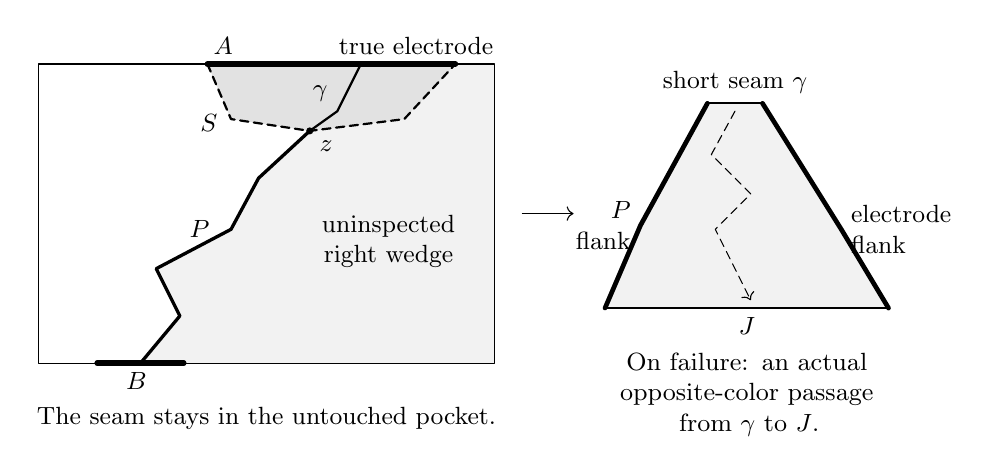
\begin{tikzpicture}[x=1cm,y=1cm,font=\small,line cap=round,line join=round]
  \path[fill=gray!10] (1.3,0) -- (1.8,.6) -- (1.5,1.2) -- (2.45,1.7)
    -- (2.8,2.35) -- (3.45,2.95) -- (4.1,3.8) -- (5.8,3.8) -- (5.8,0) -- cycle;
  \path[fill=gray!23] (2.15,3.8) -- (2.45,3.1) -- (3.45,2.95) -- (4.65,3.1) -- (5.3,3.8) -- cycle;
  \draw (0,0) rectangle (5.8,3.8);
  \draw[line width=2pt] (2.15,3.8) -- (5.3,3.8);
  \draw[line width=2pt] (.75,0) -- (1.85,0);
  \draw[densely dashed,thick] (2.15,3.8) -- (2.45,3.1) -- (3.45,2.95) -- (4.65,3.1) -- (5.3,3.8);
  \draw[line width=1.2pt] (1.3,0) -- (1.8,.6) -- (1.5,1.2) -- (2.45,1.7)
    -- (2.8,2.35) -- (3.45,2.95);
  \draw[thick] (3.45,2.95) -- (3.8,3.2) -- (4.1,3.8);
  \fill (3.45,2.95) circle (.045);
  \node[below right] at (3.45,2.95) {$z$};
  \node[left] at (2.3,1.7) {$P$};
  \node[above] at (2.35,3.8) {$A$};
  \node[below] at (1.25,0) {$B$};
  \node[left] at (2.4,3.05) {$S$};
  \node[left] at (3.8,3.42) {$\gamma$};
  \node[align=center] at (4.45,1.55) {uninspected\\right wedge};
  \node[above] at (4.8,3.8) {true electrode};
  \node[align=center] at (2.9,-.7) {The seam stays in the untouched pocket.};
  \draw[->] (6.15,1.9) -- (6.8,1.9);
  \path[fill=gray!10] (7.2,.7) -- (7.65,1.75) -- (8.5,3.3) -- (9.2,3.3)
    -- (10.2,1.7) -- (10.8,.7) -- cycle;
  \draw[line width=1.7pt] (7.2,.7) -- (7.65,1.75) -- (8.5,3.3);
  \draw[line width=1.7pt] (9.2,3.3) -- (10.2,1.7) -- (10.8,.7);
  \draw[thick] (8.5,3.3) -- (9.2,3.3);
  \draw[thick] (7.2,.7) -- (10.8,.7);
  \draw[densely dashed,->] (8.85,3.2) -- (8.55,2.65) -- (9.05,2.15) -- (8.6,1.7) -- (9.05,.8);
  \node[above] at (8.85,3.3) {short seam $\gamma$};
  \node[below] at (9,.7) {$J$};
  \node[left,align=right] at (7.65,1.75) {$P$\\flank};
  \node[right,align=left] at (10.2,1.7) {electrode\\flank};
  \node[align=center,text width=4.8cm] at (9,-.4)
    {On failure: an actual\\opposite-color passage\\from $\gamma$ to $J$.};
\end{tikzpicture}
\caption{Extending a moving electrode. Left: an actual extremal path $P$ first hits the inset cut $S$ at $z$; the small seam $\gamma$ reaches the true electrode through the untouched pocket. The tail after the last right-boundary hit, the seam, and the right outer boundary bound the protected wedge. Right: the subdisk between the seam and a farther cut $J$, drawn in abstract disk coordinates. Both flanks are wired in the tested color. Failure of their connection is an actual opposite-color hard passage with ties confined to its ends. The wedge is chosen from measured information; the future failure event is not used to condition its law.}
\label{fig:short-seam}
\end{figure}


\begin{proof}[Proof of Theorem~\ref{thm:moving-crossing}]
It suffices to prove the lower bound in each color.  In fact,
if $p$ is the separately wired probability in one color, Euler
duality gives the complementary separately wired probability
\begin{equation}\label{chordal:dual-map}
 H(p)=\frac{1-p}{1-(1-q)p}.
\end{equation}
The function $H$ is continuous and decreasing, and
$H(g(\chi))=g(1-\chi)$, using
$f(1-\chi)=1-f(\chi)$ and $q=d^2$.

Pass to any subsequence and then extract the limiting map in
Lemma~\ref{chordal:access}.  Fix a trimming margin $\beta$ and write
$\chi_\beta$ for the cross-ratio of the trimmed arcs.  Given
$\varepsilon>0$, choose the inset, then the precision and polygon,
as in Lemmas~\ref{chordal:seams} and~\ref{chordal:electrode-update},
so that the fixed polygon cross-ratio $\chi_K$ is within
$\varepsilon$ of $\chi_\beta$ and
$\limsup_n e_{n,\beta,\eta,\zeta}<\varepsilon$.
Moving both electrodes to the cuts costs at most
$e_{n,\beta,\eta,\zeta}$ in connection probability.  Each pocket factors
out through its one wire.  In the remaining disk release every
terminal link except those wiring the prescribed electrode
intervals of $K_n$; by the terminal assertion of
Lemma~\ref{pressure:network-monotonicity}, this does not increase the network probability.

Next remove the edges outside $K_n$ by cofacial peeling, which also
does not increase this particular two-terminal probability.  The geometric
justification matters here.  The two retained wire intervals are
exposed on the residual boundary and can be realized by exterior
chains.  An unwanted edge has a point outside the filled simple
polygon $K_n$, and hence an approach from an exterior gap avoiding
$K_n$.  Place an auxiliary connection-test edge across that gap
between representatives of the two terminals.  Peeling along the
approach makes each successive removed edge cofacial with the test.
The exterior chains abut $K_n$ and do not seal such a gap; their
thin realizations can be avoided.  Different gaps may use different
placements of the test edge, since after taking the chain odds to
infinity they test the same two terminals.  Isolated extra vertices
do not affect the probability.  The cofacial assertion of
Lemma~\ref{pressure:network-monotonicity} therefore gives
\[
 \PP_{T_n}(A_n\leftrightarrow B_n)
 \ge \PP_{K_n}(A'_n\leftrightarrow B'_n)
       -e_{n,\beta,\eta,\zeta}.
\]
For this fixed $K$, the exact similarity in
Lemma~\ref{chordal:seams} identifies the experiment on $K_n$ with
the compatible fixed-polygon experiment.  Theorem~\ref{thm:fixed-polygon}
therefore gives
$\PP_{K_n}(A'_n\leftrightarrow B'_n)\to g(\chi_K)$.
Taking the mesh liminf with this one polygon fixed gives
\[
 \liminf_n\PP_{T_n}(A_n\leftrightarrow B_n)
 \ge g(\chi_K)-\limsup_n e_{n,\beta,\eta,\zeta}
 \ge g(\chi_K)-\varepsilon.
\]
For fixed $\beta$, this construction is available for every
$\varepsilon>0$, and $|\chi_K-\chi_\beta|<\varepsilon$.
Continuity of $g$ therefore gives the lower bound
$g(\chi_\beta)$ as $\varepsilon\downarrow0$.  Each application
of the fixed-polygon theorem used one polygon held fixed during its
mesh limit; no uniformity over polygonizations is required.
Finally let $\beta\downarrow0$ and use continuity once more.
Apply the same argument in the other
color and use \eqref{chordal:dual-map} for the upper bound.
One-slot endpoint changes have vanishing chart size by
Lemma~\ref{chordal:access}, so are absorbed by the angular margins.
The sequential argument proves the asserted uniformity.
\end{proof}

\subsection{A drawing compatible with the finite law}

We specify the discrete representation before applying the moving
formula to a stopped interface.  No change to the finite law in
Theorem~\ref{thm:main} is made.

\begin{lemma}[A gapped simple drawing]\label{chordal:drawing}
At the initial drawing interface, let $D_\delta$ be the bounded
interior of a simple closed nearest-neighbor polygon in $\delta\Z^2$, and
let $a_\delta,b_\delta$ be distinct vertices of that polygon.
Use the full graph of vertices and edges in the closed polygon.
The wired arc is a closed boundary arc including both marked vertices.
Every graph edge is sampled in the law, and exactly the boundary edges of that arc are
declared open for the prescribed drawing.  For this graph and law
in Theorem~\ref{thm:main}, there is a tiled topological disk $V_\delta$
with injectively embedded interior and a rounded strand with the
following properties.  Below we write $V=V_\delta$ when the mesh is fixed.
\begin{enumerate}[label=(\roman*)]
\item The marked boundary tracing of $V$ is at distance $O(\delta)$
from that of the original polygon.  The rounded strand's actual
medial boundary endpoints $a_\delta^V,b_\delta^V$ are within
$O(\delta)$ of $a_\delta,b_\delta$, respectively.  Along a uniformly
convergent marked Jordan sequence, fix $z_*\in D$.  Eventually
$z_*\in V_\delta$, and the inverse disk maps
\[
 F_\delta:\D\longrightarrow V_\delta,\qquad
 F_\delta(0)=z_*,\qquad F_\delta'(0)>0
\]
converge uniformly on the closed disk to the correspondingly
normalized map $F:\D\to D$.  The preimages of
$a_\delta^V,b_\delta^V$ converge to those of $a,b$.
\item The rounded strand is simple, lies in $\operatorname{int}V$
except at its two endpoints, and matches the ordered local pieces
of the prescribed medial strand at curve distance $O(\delta)$.
It uses polygonal templates with uniformly nondegenerate angles
and gaps at least $c\delta$ between nonincident pieces, and between
the inner drawing and the wall except at endpoint transversals.
\item At a switch-revealing stop its unknown original edges have
the ordinary conditional FK law, with known open edges contracted
and known closed edges deleted.  Bank sites have access to the
corresponding side of the prefix within physical diameter $O(\delta)$.
Designated boundary slots have simultaneous short outward accesses
to their own intervals.
\item The same construction is available for four open changes.
Separate deterministic closure in a tested color changes the
conditional open pairing probability $p$ into
\begin{equation}\label{chordal:cap-odds}
 p\longmapsto\frac{p}{p+d(1-p)}.
\end{equation}
The drawings and normalization can be kept identical away from an
interval on which an extra pair of changes is inserted.
\end{enumerate}
All accesses and gaps refer to the appropriate disk sectors at slit
contacts; they do not pass through a wall to another incidence.
\end{lemma}

\begin{proof}
Use one full checkerboard tile for each graph edge, including its
exterior triangular tab when it is a boundary edge.  Within each
ordinary square, glue its four incident triangles across their
matching port sides.  Do not glue different exterior tabs along
their radial sides.  Simplicity of the initial polygon gives one
interior polygon fan at each boundary vertex.  A primal boundary
vertex retains that fan and the tabs at its two extreme edges.
Tile interiors
and glued-side interiors are disjoint under planar projection;
additional coincidences occur only on boundary incidences.
A concave fan can have full angle $2\pi$, in which case its extreme
sides form a slit rather than being identified.  The result is a
topological polygonal disk.  Its boundary follows the original
boundary with detours of diameter $O(\delta)$.

The assumed closed counterclockwise boundary parametrizations trace
once, are injective on $[0,1)$, and converge uniformly with their
marked cyclic parameters.  The compression below preserves this
tracing order and moves the boundary by $O(\delta)$.  Uniform
parametrized convergence to a simple Jordan boundary
implies uniform local connectedness of these boundary images:
nearby image points have nearby parameters, up to the short
detours, and are joined along a boundary segment of uniformly small
diameter.  Kernel convergence and the boundary extension criterion
then give uniform convergence of normalized inverse maps on the
closed disk.  The side-interior endpoint transversals are within
$O(\delta)$ of the marked polygon vertices.  Uniform convergence
of the boundary maps and injectivity of the limiting Jordan map
therefore give the claimed convergence of their preimages.
Repeated boundary incidences still use their own prime sectors.

Slightly compress the tile complex into $V$, leaving a thin collar
for the cap arcs and unmatched-port extensions; denote this
compression by $\sigma$.  Draw each switch by two disjoint simple
turn arcs toward the corresponding corners, avoiding both those
corners and the opposite boundary diagonal.  On a designated
interval use the local caps between successive visits of its color;
an unassigned slot is capped around between its two incident ports.
A designated slot has a short outward access between caps; the
outward access from an undesignated slot crosses just its surrounding
cap.  At a change leave the appropriate port unmatched and extend
it to a side-interior boundary point by an initially perpendicular
straight segment.  These are the only contacts of a chord with the wall.

Here the compression and arcs can be chosen from finitely many
polygonal templates.  Inset each boundary edge in a strip and each
vertex within its abstract fan, matching by a fixed subdivision of
the adjacent tiles, and leave $\sigma$ unchanged off an
$O(\delta)$ boundary neighborhood.  Fans have at most full angle
$2\pi$.  At coincident slit sides make the offsets on their
respective inset sides.  Ports lie away from side endpoints and
arcs meet there transversely.  There are only finitely many scaled
local configurations of fans, caps, changes, and switches, so the
choices give uniform positive gaps and angle bounds.  In particular,
an interior access of diameter $o(\delta)$ near a join can encounter
only its local incident pieces; it cannot confuse opposite slit
half-neighborhoods.  Every piece length and displacement is
$O(\delta)$.  The compression is used only for drawing, not as a
conformal map.

The positive loop identity follows directly in this representation.
Draw planar exterior trees for the separate tested wires and thicken
the open graph together with these trees.  If $\ell$ is its number
of perimeter components, Euler's formula gives
\[
 \ell=2k(A)+|A|+\text{a constant independent of }A.
\]
Consequently $d^\ell$ is proportional to
$q^{k(A)}d^{|A|}$, the finite FK weight.  This calculation uses only
$d>0$.  Conditional component counting gives the same statement
after revealing switches, with the induced contractions and deletions.

At an originally wired boundary edge, its endpoints were already
identified, so its sampled state is an independent loop variable
for weighting.  The exterior dual cap joins its inner continuations
in the same way in either state.  Declaring the edge open for the
prescribed drawing replaces a bounded-size cap detour and possibly
removes a microscopic closed loop.  On the free arc, the cap around
a primal singleton is the boundary turn beside the dual wired arc.
Match the remaining pieces in their occurrence order.  Simultaneous
parametrizations differ by $O(\delta)$, including at a medial point
visited with two different pairings; constant pieces are handled
by limits of increasing homeomorphisms.  This proves the drawing
claim in exactly the curve metric of Theorem~\ref{thm:main}.

Along a known bank, a revealed diagonal of that color connects its
two sites, and a turn around a site of that color stays at that site.
A cap stays at one site or follows consecutive sites of its designated
wire.  Thus each bank is attached to its original electrode and has
the claimed local accesses.  The two color accesses at a tile can
be drawn on their respective sides of the turn, simultaneously
with the designated slot accesses in the collar.

With four open changes there are two noncrossing pairings.  Under
separate tested-color closure, the connection alternative adds one
completed loop and its complement adds two.  Their full-sample
relative weights are therefore $d$ and $d^2$.  Conditioning that
full density on any history gives \eqref{chordal:cap-odds}; it is
not a limiting domain Markov assertion.  The density and its
reciprocal are bounded in terms of the fixed $q$.  In the two-change
case the pairing is forced and closure introduces no bias.
Insertion changes only the local caps and designations near the
new interval, so the rest of the drawing may be left unchanged.
\end{proof}

\subsection{Eroding a revealed prefix}

\begin{lemma}[Remaining tiled pieces]\label{chordal:erosion}
Stop the rounded strand at a local piece junction, with the states
of all encountered switches known but no unused next step specified.
Let $U$ be $V$ slit along its simple prefix.  There is a collection
of remaining tiled disks with cut-triangle cells such that:
\begin{enumerate}[label=(\roman*)]
\item Their compressed interiors are disjoint open subsets of $U$.
Every point outside these interiors, including their boundaries,
has a path of diameter $O(\delta)$ to the prime boundary of $U$
outside the piece interiors.
\item For a fixed color, the only interactions between pieces are
the original wires and the ties supplied by known banks.  A
non-dummy site with different remaining fan occurrences is already
tied to a known bank.  Every untied site has its complete remaining
incident fan in one piece.
\item On a half cell cut along a measured open diagonal, its color
endpoints are tied and the opposite-color virtual midpoint is free.
One may resample the half-cell state at the ordinary input odds
without changing unknown original-edge laws or terminal probabilities.
\end{enumerate}
These assertions also hold after advancing a stop by boundedly many
local pieces, with short accesses measured in the original stopped
disk.  New bank contacts from that advance access the old tip within
$O(\delta)$.
\end{lemma}

\begin{proof}
Use the uncompressed tile geometry to perform the following erosion.
For a visited turn remove the triangle on that side of the revealed
diagonal, namely the triangle containing the corner turned around.
If both turns have been visited, remove both triangles.  Retain a
remaining triangle as a cut-triangle cell and split every corner
into its remaining connected sectors.  The resulting pieces are
connected through their still glued sides.

Successive removed triangles connect through the crossed port sides
back to the beginning of the prefix on the exterior boundary.
Segments ending at a visited outer cap also connect to the exterior.
Thus there is no isolated removed component enclosing a hole.
More explicitly, in the complement of the regular open interior of
a retained component every removed cell is connected to the exterior
by such a chain; any other retained component adheres to these
chains or the outer boundary.  That complement is connected.
Splitting disconnected corner fans makes each retained component a
compact polygonal surface with simply connected interior and hence
a topological disk.  Its uncompressed interior remains injectively
embedded in the original grid.

Every previously crossed port, except possibly the current tip
junction, has both continuation triangles removed, or borders a cap
and a removed triangle.  Hence a compressed piece meets the measured
strand only at an exposed used port at the current end.  From a
removed triangle one can approach its visited turn on the relevant
side within that triangle; if another removed region is encountered
first, use its first boundary encounter.  A cut diagonal has the
same access through its removed triangle.  Collar points have the
corresponding cap or wall access.  This proves the first assertion
with the indicated disk incidence at contacts.

The bank-chain description in Lemma~\ref{chordal:drawing} shows
that a measured diagonal of the tested color is already contracted
to that bank's wire.  Its opposite-color midpoint is a new free
dummy slot.  The diagonal can therefore be sampled independently
as a loop at the ordinary odds.  From the opposite-color viewpoint
the spoke only dangles, and its opening odds after the component
factor are $v/q$, with input odds still $v$.  Integrating it out
does not change any other state or terminal event.  This explains
the half-cell convention without claiming a new drawing inside an
already measured cell.

If an ordinary color site has two disconnected remaining sectors,
some removed triangle at that corner has put the site on a known
bank.  Conversely an untied site has no such removed corner sector,
so its available incident fan is still connected in one piece.
The original weights conditioned on the history depend on unknown
edges only through component counts after contraction of known
open paths and the original wires.  Thus shared tied sites and
these wires exhaust all interactions between the pieces.

Finally, a bounded local advance removes only boundedly many
additional triangles or collar pieces, all adjacent to the old tip
or the portion just traversed.  Their exterior accesses run back
through these discarded strips to the old tip within $O(\delta)$.
No unrelated state need be queried.  The same assertions therefore
hold with accesses taken in the original stopped disk.
\end{proof}

\begin{proposition}[The localized stopped four-change test]
\label{prop:slit-test}
Fix $q\in(0,1)$ and $r_0,s_0,M>0$.  Let
$\mathcal H_\delta(r_0,s_0,M,q)$ consist of the following data:
a rounded four-open-change experiment from
Lemma~\ref{chordal:drawing} at mesh $\delta$ with $V\subset B(0,M)$;
a compatible history $\omega$ of its strand at a path-adapted
stopping time $\tau$,
from the original first mark, before completion and revealing only
encountered switches; and a point $z$ such that $B(z,r_0)\subset U$,
where $U$ is the remaining slit disk.  Require the tip and the three
remaining marked prime ends to have pairwise Euclidean distance at
least $s_0$ in a disk chart $\varphi_U:U\to\D$ with $\varphi_U(z)=0$.
The condition is independent of the chart's rotation.  If $E$ is
the tested-color pairing alternative and $\chi_U$ is the current
ordered cross-ratio, then
\begin{equation}\label{chordal:stopped-test}
 \varepsilon_{\rm stop}(\delta;r_0,s_0,M,q)
 :=\sup_{\mathcal H_\delta(r_0,s_0,M,q)}
 \left|
 \PP_{\rm open}(E\mid\mathcal F_\tau)(\omega)
       -f(\chi_U(\omega))
 \right|
 \longrightarrow0\qquad(\delta\downarrow0).
\end{equation}
An empty supremum is zero.  The class includes stops inside local pieces.
\end{proposition}

\begin{proof}
First restrict to junction stops.  If the stated supremum did not
tend to zero for that subclass, choose $\delta_n\downarrow0$ and
data from the class whose errors stay bounded away from zero.
Write $U_n$ for their slit disks and normalize their disk charts at
the chosen basepoints.  Pass to a subsequence on which the four
marked chart positions converge; their limits remain distinct by
the fixed separation.  We prove convergence along this sequence.
The required reduction has three parts: find the one remaining tiled
disk carrying the macroscopic chart, match its boundary incidences to
the stopped chart, and identify its conditional law as a two-terminal
law up to arbitrarily small angular margins.

\paragraph{The two terminals remain distinct.}
Use separate closure in one color.
There is no contact of its known bank with the other electrode of
that color under the stated localization.  Indeed, until a first
such contact, the bank is attached to its starting electrode.
At a purported contact the site has simultaneous short accesses
to that bank side and to the distinct original electrode, by
Lemma~\ref{chordal:drawing}.  Their concatenation is a connected
physical access of diameter $O(\delta)$ with chart endpoints in
separated intervals, contradicting Lemma~\ref{chordal:access}.
A visit to another electrode through a cap has the same property.
Thus the two terminal wires remain distinct.

\paragraph{One remaining piece carries the disk chart.}
Erode the history as in Lemma~\ref{chordal:erosion}.  In the
$U_n$ chart every fixed compact subset of $\D$ eventually belongs
to a single compressed piece, denoted $T_n$.  Interior distortion
at the thick basepoint gives a fixed positive physical clearance
for such a compact set, whereas all removed cells and boundary
deformations are within $O(\delta)$ of a wall or queried tile.
The short accesses from the exterior of the pieces have chart
diameter $o(1)$.

Every other piece has chart diameter $o(1)$, uniformly, including
its boundary accesses.  Otherwise, since the other pieces avoid
every fixed chart compactum, one contains a path spanning a polar
rectangle of fixed angular width in an outer annulus.  Select a
subpath joining its radial sides and staying between them.  The
middle radius from the core of $T_n$ must meet this subpath before
reaching the unit circle.  Its first exit from $T_n$ occurs earlier,
on the inner side of the spanning subpath.  From that exit, the
short exterior access supplied by erosion reaches the unit circle
without entering any piece interior.  Its chart diameter is $o(1)$,
so it stays between the two radial sides.  It must therefore cross
the spanning subpath to reach the outer boundary, contradicting
that subpath's location in another piece interior.
This proves the assertion without assuming physical boundary
regularity of the stopped domains.

\paragraph{Match the boundary incidences, not only the kernels.}
The normalized chart of the \emph{uncompressed} tiled disk $T_n$
agrees, also on its boundary incidences, to $o(1)$ with the ambient
$U_n$ chart of its compressed image.  We give the details because
interior kernel convergence alone would not suffice here.
On chart compacta the erosion and compression do nothing.  Thus
the pointed kernels agree and the normalized charts match in the
interior.  Conversely, any fixed cleared path with spare-width
neighborhoods in the main piece remains in the slit-disk kernel:
its $O(\delta)$-displaced embedded neighborhoods surround a
slightly smaller tube, by injectivity and degree.  These observations
give the two-sided interior kernel assertion.

For boundary matching, choose finitely many well-spaced marker
angles in the piece chart.  Close to each marker select a ray with
a short physical terminal segment from radius $1-\eta$ to the
piece boundary, using Lemma~\ref{chordal:access}(ii).  Avoid the
finitely many vertex coincidences.  Continue its compressed endpoint
to the boundary of $U_n$ by the short exterior access, trimmed not
to reenter the piece.  Interior matching and
Lemma~\ref{chordal:access}(i) keep each combined access in a small
angular neighborhood of its marker in the $U_n$ chart.  The accesses
can be trimmed to disjoint crosscuts in their separate windows.
Together with the embedded inset circle, they separate the sectors
between consecutive markers.  The sector between two consecutive
marker rays is connected in the piece chart, and its compressed image
remains connected: compression is an embedding, although it need not
be conformal.  The two rays, their exterior continuations, and the
inset-circle arc bound its side in $U_n$.  Approach a boundary
incidence of this sector from its interior.  Its image cannot cross
either bounding access, so its ambient chart position lies between
the same two small marker windows.  The short exterior accesses also
put all compressed piece-boundary points within $o(1)$ of the unit
circle in the ambient chart.  First take $\eta$ small for the chosen finite
partition, and then refine the partition.  This proves uniform
boundary-coordinate matching, with incidence limits from the open
sectors, without extending a map uniformly to a rough limiting slit.

\paragraph{Identify the terminal law and apply the moving formula.}
All tested-color sites tied to an electrode have short accesses to
its corresponding prime interval in $U_n$.  Conversely, a boundary
slot of $T_n$ whose matched chart position is strictly inside a
tested electrode sector is attached to that electrode.  On a
cut-triangle side its position is within $o(1)$ of the known open
color side of the slit, by the removed-triangle access; it is then
a tied endpoint, not a free virtual slot.  On an original side,
an undesignated slot has access to another color interval unless
a visited cap blocks it, in which case it is attached to the
corresponding prefix bank.  The current tip is a change, and fixed
angular margins absorb its one-cell neighborhood and all slot
rounding.  This gives the exact two-terminal classification away
from vanishing chart margins.

No small-chart exterior piece can touch both separated terminals.
By Lemma~\ref{chordal:erosion}, unknown edges belong to their one
piece; any shared site is already on one of the same wires; and
all known links have exposed slots on the piece boundaries.
Consequently an exterior piece attaches through at most one hub.
Its partition function factors out as a multiplier independent of
the remaining edge states.  There is neither an already achieved
bridge nor an unaccounted connection between distinct terminals.
This is an exact factorization of the conditional finite law; the
vanishing chart diameters were used only to rule out attachment to
both terminals.

For an arbitrarily small fixed angular margin, shrink or enlarge
the two electrode intervals on $T_n$ by that margin.  The actual
set of its tied boundary slots lies between the two choices.
The terminal assertion of Lemma~\ref{pressure:network-monotonicity}
sandwiches the global conditional connection
probability between the resulting pure two-terminal probabilities.
Apply Theorem~\ref{thm:moving-crossing}, let the margin shrink, and
undo \eqref{chordal:cap-odds}.  Continuity of $g$ at the four
distinct limiting chart positions proves convergence along the
chosen sequence, contradicting its error bound.  This proves
\eqref{chordal:stopped-test} for junction stops.

\paragraph{Average back to a stop inside a local piece.}
For an arbitrary sequence of stops inside local pieces, reveal
through the next turn
junction, advancing by only boundedly many local pieces.  The
extra slit has chart diameter $o(1)$ and attaches at the current
tip.  Removing a notch of vanishing diameter changes the normalized
coordinates of all four marks by $o(1)$: fixed separating crosscuts
away from the notch give boundary convergence there, and neighboring
marker intervals squeeze the new tip.  Thickness and separation
therefore persist, eventually with margins $r_0/2$ and $s_0/2$.
No remaining marked port can be reached in that local advance.

Decide only switches encountered in traversing those pieces,
including a previously measured tile if revisited; do not condition
on an unused next turn.  The junction conclusions then average in
their respective laws.  In particular the exact cap-odds conversion
is first made at each junction under its full-sample conditional
density, and the open-law conclusions average to the open-law
conditional probability at the original stop.  This proves the
statement for every path-adapted stopping rule.
\end{proof}

\subsection{Unforced quadrilaterals and curve compactness}

We use crossing modulus in the convention that $(0,L)\times(0,1)$,
crossed between its vertical sides, has modulus $L$.
An \emph{avoidable quadrilateral} in a stopped slit domain has its
longitudinal sides on the prime boundary and does not disconnect
the current tip access from the target access.  A crossing means
a traversal between its two open ends by a subarc of the future curve.

\begin{theorem}[Uniform unforced-crossing estimate]\label{thm:c2}
For the sufficiently fine rounded Dobrushin interfaces of
Lemma~\ref{chordal:drawing}, the conditional probability of crossing
an avoidable quadrilateral tends uniformly to zero as its crossing
modulus tends to infinity.  Uniformity includes the mesh, every
stopping time before completion, every compatible stopped history,
and every such quadrilateral in the remaining prime-end domain.

For a marked domain approximation of Theorem~\ref{thm:main}, the
interfaces, transported to a fixed marked disk, consequently
satisfy Condition C2 of \cite{KemppainenSmirnov2017}.  They are
jointly subsequentially compact as oriented curves modulo increasing
reparametrization and through their half-plane driving functions
on compact capacity intervals.  Every joint limit is a continuous
Loewner-generating curve with the limiting driver, is parametrizable
by strictly increasing capacity until the target, and has no
additional time-ordered excursions omitted by this description.
The target is reached only at completion.  Curve compactness also
holds in the original physical coordinates.
\end{theorem}

\begin{proof}
All boundary statements are in disk topology, so distinct incidences
at a slit or pinched projected boundary remain distinct.  After
cropping the open ends, the two longitudinal flanks of an avoidable
quadrilateral belong to the same open boundary interval between
the current tip and target.  Otherwise an interior transverse
crosscut joining opposite tip--target intervals would separate
the two marked accesses, contrary to avoidability.  Thus one color
has no designated boundary interval on either flank.  Call this
the tested color.

It suffices to consider arbitrary sequences of meshes, stopped
histories, and avoidable quadrilaterals whose crossing moduli $L$
diverge, and to show that their conditional crossing probabilities
tend to zero.  An impossible crossing has probability zero, so
assume each experiment has a compatible crossing continuation.
Cropping to regular interior subbands preserves the necessity of
traversal and leaves a central rectangle of length comparable to
$L$.  This also accommodates arbitrary original open ends.  Under
conformal transport the same tests can be made in the prime disk;
the prelimit slit boundary accesses used below are polygonal.

\paragraph{A small crosscut and a distant crosscut.}
Uniformize the quadrilateral by $(0,L)\times(0,1)$.  For
$x\in[L/4,3L/4]$, let $C_x$ be the physical image of the vertical
crosscut, including its two prime-boundary endpoints.  Choose $C_i$
with diameter $w>0$ at most twice the infimum of these diameters,
and choose $z\in C_i$.  Every crosscut in this central range then
has diameter at least $w/2$.

Put $K=L^{1/8}$.  For sufficiently large $L$ some $C_j$ lies
wholly outside $B(z,Kw)$.  Otherwise each central crosscut has
arclength at least $cw$ inside $B(z,(K+2)w)$: either it stays in
that enlarged ball, or a segment from its visit to the smaller
ball travels a distance comparable to $w$ before leaving the
larger one.  If $F$ is the conformal parametrization in physical
coordinates, Cauchy--Schwarz on the verticals gives
\[
 c^2w^2\frac L2
 \le \int_{L/4}^{3L/4}\int_0^1
 |F'(x+\ii y)|^2
 \one_{\{|F(x+\ii y)-z|<(K+2)w\}}\,\dd y\,\dd x
 \le \pi(K+2)^2w^2.
\]
Injectivity in the embedded physical interior gives the last bound;
coincident boundary projections do not affect area.  This
contradicts $K=o(\sqrt L)$.

\paragraph{Excluding submesh transverse passages.}
On a sequence with a possible crossing, $w/\delta$ is bounded away
from zero after discarding finitely many terms.  If not, pass to
a subsequence with $w/\delta\to0$, and let a compatible future
crossing meet $C_i$ at $p$.  The two parts of $C_i$ give accesses
of diameter at most $w$ from $p$ to its boundary endpoints.

The finite gapped templates of Lemma~\ref{chordal:drawing} describe
all these submesh encounters.  A future strand approaches its past
at this scale only on consecutive local pieces, within strand
arclength $O(w)$ of the current tip.  An approach to the original
wall occurs only on an initial or final transversal, within
arclength $O(w)$ of its attachment.  In the initial case the stop
itself is within that distance of the initial attachment.
Nondegenerate template angles make these arclength bounds uniform.

Thus each endpoint of $C_i$, on its containing tip--target interval,
is within boundary arclength $O(w)$ of the tip or target.  If the
encounters use different marks, $p$ is within remaining strand
arclength $O(w)$ of both the current tip and target.  Only $O(w)$
arclength remains, making a visit to $C_j$ impossible.  If both
endpoints are near the same mark, use boundary order on their common
tip--target boundary interval.  The mark-free intervals cut off by
$C_i$ and $C_j$ are nested, since these are transverse sections of
one quadrilateral.  If the $C_j$ interval lies inside the $C_i$
interval, both its endpoints remain within boundary arclength $O(w)$
of the mark.  If it contains the $C_i$ interval, its endpoint nearer
the mark lies between that mark and the nearer endpoint of $C_i$,
so the same bound holds for that endpoint.  It is then within physical
distance $O(w)$ of $C_i$, again contradicting the choice of $C_j$.
The argument includes stops in the middle of a local piece.

\paragraph{Erosion and protected radial ranges.}
Keep the original stopped slit $U$ fixed.  Condition further on
the encountered states needed to advance to the next local turn
junction, as in Lemma~\ref{chordal:erosion}.  This advances only
$O(\delta)$ and queries no unrelated state.  Newly exposed piece
boundaries and attachments access the original tip within
$O(\delta)$.  If only a final short transversal remains, it cannot
traverse from $C_i$ to $C_j$.  Uniform bounds after this local
advance imply the same bound before it by conditional averaging.

Let $B$ be the subband between $C_i$ and $C_j$, and set
\[
 s=wK^{1/3},\qquad t=wK^{2/3}.
\]
Then
\[
 \delta\ll s,\qquad w\ll s\ll t\ll Kw,
 \qquad t/s\longrightarrow\infty.
\]
In fixed-factor neighborhoods of the physical levels $s$ and $t$
about $z$, a path of diameter $O(\delta)$ in $U$ cannot reach
either end of $B$.  Any short boundary access there therefore
reaches only its flanks; it cannot reach a tested-color designation
or the tip.

There are transverse polygonal crosscuts of $B$ in narrow
neighborhoods of these two levels.  The physical level separates
the ends, and disk path/cut separation gives a flank-to-flank
connection in that separating set.  A narrow neighborhood permits
an interior polygonal crosscut with the same separation property.
The stopped boundary is polygonal in its slit incidences, and
all subsequent perturbations stay in buffered radial ranges.

\paragraph{Selecting fixed tiled cuts.}
We now construct two cuts from the stopped data alone.  A compatible
completion will certify their geometry; the conditional law will not
be restricted to that completion or to successful crossings.
A compatible future traversal has a tested-color bank shadow.
In a protected region it uses actual available edges, not boundary
identifications.  An untouched turn either stays at its tested
corner or uses its actual open diagonal.  In a retained half tile,
the unvisited turn stays at the free corner when that color is
missing from the flanks.  A cap similarly stays at its slot.
A jump between designated tested-color sites, or a contact with
an already tied tested site, would give a forbidden short access
to that designation or the original tip.  Untied site fans have
consistent incidences in one eroded piece by
Lemma~\ref{chordal:erosion}.  The shadow can therefore be perturbed
into piece interiors.

Choose one compatible crossing continuation deterministically from
the fixed conditional data, solely as a geometric witness.  Its
shadow gives an end-to-end continuum in $B$ lying in piece interiors
throughout the two protected radial ranges, spliced to the rest of
the traversal outside those ranges.  For example, order the finitely
many completions and choose the first one giving a crossing.
This choice reveals no additional switch, and we do not condition
the law on this continuation occurring.

Take a transverse polygonal crosscut near radius $s$.  Every point
on it outside all piece interiors has a short access, outside those
interiors, to a flank.  It cannot have such accesses to both flanks:
their union would give a transverse connection disjoint from the
witness continuum.  The label is also constant on each connected
segment outside the piece interiors: a segment with differently
labeled points, concatenated with their flank accesses, would give
the same forbidden transverse connection.  After a general-position
perturbation, the crosscut has a finite alternating decomposition
into such complementary segments and intervals inside individual
pieces.  Its endpoint labels differ.  Reading this decomposition
from one end, the first change of label must therefore occur across
an interval in one piece, whose two boundary contacts have opposite
flank labels.

Replace the selected piece interval by a tile-edge path within
$O(\delta)$ of it.
Consecutively encountered tiles join along their sides; within a
half triangle its two tile sides connect the corners.  Move boundary
contacts to corners within their cells as well.  These moves remain
protected.  No boundary edge connects opposite labels, since its
short exterior accesses would contradict the same witness separation.
Take the last contact of one label and the first ensuing contact
of the other, and erase loops.  This gives a proper simple tile-edge
crosscut $\gamma_s$ in that piece.  Prolong its endpoints outside
all piece interiors to the two flanks.  The prolongations can be
chosen disjoint: an intersection would make the excluded
complementary flank-to-flank connection.  The resulting proper
crosscut $\Gamma_s$ of $U$ separates the ends of $B$.
Construct $\gamma_t$ and $\Gamma_t$ in the same way.  Their radial
ranges are disjoint.  These cuts are now fixed for the conditional
law, not chosen anew from each crossing sample.

\paragraph{One piece, including physically folded regions.}
Let $M$ be the middle component between $\Gamma_s$ and $\Gamma_t$.
By prime-boundary order, $M\subset B$.  Every short boundary access
from $M$, or a sufficiently small short-path neighborhood of it,
remains protected.  In fact, an access leaving $B$ through $C_i$
or $C_j$ must first meet a separator, which is still at distance
much greater than $\delta$ from that end.  This contradicts the
access having diameter $O(\delta)$.  The reasoning remains valid
when parts of $M$ fold physically close to an end without having
a short access to it.

Every crossing sample therefore has an actual tested-color bank
lift throughout its passage across $M$.  Start and end the lift
a large fixed multiple of $\delta$ beyond the respective separators,
using their buffers.  Its interior perturbation cannot meet the
outer prolongations, which lie outside all piece interiors.
It crosses $\gamma_s$ and $\gamma_t$ and remains in one piece.
Thus the two predetermined cuts belong to the same eroded disk
whenever a crossing is possible.  The untied-fan assertion prevents
a passage between pieces through a split vertex or pinched incidence.

The middle tiled subdisk $T$ between these two cuts embeds into
$M$: its interior misses the outer prolongations and adjoins both
cuts.  Orient the bank path from the near cut to the far cut, and
retain its segment after the last near-cut visit and before the
first subsequent far-cut visit.  This is an actual tested traversal
of $T$.  Let the interior perturbation tend to zero;
the hits then use cut corner vertices, since color bonds meet
tile-edge cuts only there.  Intermediate boundary contacts can
be trimmed without changing the traversal.

\paragraph{The conditional law on the subdisk.}
Condition additionally on the states outside $T$.  At a non-end
flank site, every available incident edge belongs to this piece
and middle subdisk.  A shared split occurrence or previously
wired tested site would instead give a forbidden short access
to a known bank or designation.  Thus even an outside path that
returns from far away cannot attach to a non-end flank: it has no
available first edge there.  Physical proximity of folded portions
does not add graph incidences.  Hence the exterior induces
identifications only on the two end cuts.  They form a planar
partition, since the measured links, original closure, and outside
state connections are planar.  At repeated contacts, slightly
separate incidences inward to read their cyclic order.  Retained
half cells and dummy spokes have exactly the harmless conventions
of Lemma~\ref{chordal:erosion}.

The near cut lies within $O(s)$ of $z$, and the far cut is at
distance comparable to $t$.  Compression changes these distances
only by $O(\delta)$.  Theorem~\ref{thm:actual-disk} bounds this
actual traversal uniformly by a quantity tending to zero, since
$s/\delta\to\infty$ and $t/s\to\infty$.  Its uniformity over
arbitrary joint planar end partitions, without a bound on their
number of contacts, allows averaging over all outside
states and then over the junction advance.  Every quadrilateral
crossing required the traversal.  This proves the bound for every
sequence with diverging modulus, hence the uniform assertion.
In particular, a sufficiently large modulus gives conditional
probability at most $1/2$.

\paragraph{Compactness and completion.}
For clarity, the form of the external theorem we use is the
following: a family of simple interior chords in a fixed marked
disk satisfying that last bound for all stopping times and all
avoidable quadrilaterals satisfies Condition C2.  Proposition 2.6,
Theorem 1.5, and Corollary 1.7 of
\cite{KemppainenSmirnov2017} then give joint tightness of oriented
curves and compact-time uniform drivers, with compatible generating
limits.  The limiting curve reaches its target only at completion,
and capacity is strictly increasing before it.  These are geometric
theorems about curves, not FK crossing inputs.

Lemma~\ref{chordal:drawing} supplies precisely the required simple
interior chords.  For each fixed mesh, sending the target to infinity
makes capacity run to infinity: the final transversal reaches a
smooth side-interior attachment nontangentially, so its half-plane
image has unbounded height.  The driver conclusions therefore apply
on every compact capacity interval.  Finally, the uniformly
convergent extensions of the initial inverse maps transport curve
convergence from the marked disk to physical coordinates.
The $O(\delta)$ drawing comparison transfers the compactness
statement to the prescribed interfaces.
\end{proof}

\subsection{Two bounded martingales identify the driver}

Conditional probabilities of the auxiliary pairing event are exact
martingales.  The stopped four-change formula identifies their
scaling limit.  We will insert a short boundary electrode, determine
its small-interval asymptotic, and transfer a bounded normalization
of the martingale to the ordinary Dobrushin law.  Two insertion
locations then determine both characteristics of the driver.

\begin{lemma}[The small-interval exponent]\label{chordal:small-interval}
For the function $f$ in \eqref{chordal:functions},
\[
 f(\chi)=c_q\chi^h(1+o(1))\quad(\chi\downarrow0),
 \qquad c_q>0.
\]
\end{lemma}

\begin{proof}
For $\chi<1/4$, split $I_B$ at $1/2$.  The upper integral is
uniformly bounded, since its only remaining singularity has
exponent $1-3\rho>-1$.  In the lower integral substitute $u=\chi z$:
\[
 \chi^h\int_\chi^{1/2}
 u^{\rho-1}(u-\chi)^{\rho-1}(1-u)^{1-3\rho}\,\dd u
 =\int_1^{1/(2\chi)}
 z^{\rho-1}(z-1)^{\rho-1}(1-\chi z)^{1-3\rho}\,\dd z.
\]
On this range the last factor is bounded by $2^{3\rho-1}$.
The remaining function is integrable at $1$ and infinity, since
$\rho-1>-1$ and $2\rho-2<-1$.  Dominated convergence gives
\[
 \chi^h I_B(\chi)\longrightarrow
 J_\rho:=\int_1^\infty z^{\rho-1}(z-1)^{\rho-1}\,\dd z
 \in(0,\infty).
\]
Likewise $I_C(\chi)\to I_C(0)\in(0,\infty)$: at $u=1$ its
exponent is $1-3\rho>-1$, and at infinity it is $-1-\rho<-1$.
Equation~\eqref{chordal:functions} now proves the claim with
$c_q=I_C(0)/J_\rho$.  The substitution $z=t/(t-1)$ identifies
$J_\rho=I_C(1-)$, whose exponent at $t=1$ is $-2\rho>-1$.
\end{proof}

\begin{proposition}[Identification of the driver]\label{prop:driver}
Every subsequential joint limit supplied by Theorem~\ref{thm:c2}
from a marked domain approximation of Theorem~\ref{thm:main}
has half-plane driving process
\[
 W_t=\sqrt\kappa B_t,\qquad
 \kappa=\frac4{1-\rho}=\frac{4\pi}{\pi-\lambda},
\]
where $B$ is standard Brownian motion in the natural driver filtration.
\end{proposition}

\begin{proof}
Fix $z_*\in D$ as in Lemma~\ref{chordal:drawing}.  For each rounded
initial domain use the unique conformal map
\[
 \phi_\delta:V_\delta\longrightarrow\H,\qquad
 \phi_\delta(a_\delta^V)=0,\quad
 \phi_\delta(b_\delta^V)=\infty,\quad
 \Im\phi_\delta(z_*)=1.
\]
Use the analogous normalization $\phi:D\to\H$ at $a,b,z_*$.
The uniformly convergent inverse disk maps in
Lemma~\ref{chordal:drawing}, together with convergence of the two
marked preimages, imply convergence of the associated
disk-to-half-plane M\"obius normalizations.  Consequently
$\phi_\delta^{-1}\to\phi^{-1}$ uniformly on
$\overline\H\cup\{\infty\}$, with its spherical topology, as maps
to the physical closed domains.  This fixes the residual positive
scale in the initial half-plane charts.

Use the color whose positive real boundary side is free.
Write $g_t$ for the hydrodynamically
normalized maps, so that
\[
 \partial_tg_t(z)=\frac2{g_t(z)-W_t},\qquad g_0(z)=z.
\]
The prelimit maps and drivers below refer to these rounded simple
drawings and charts.  Fix $T<\infty$, $R>0$, and $x>2R+1$, and stop at
\[
 \tau_R=T\wedge\inf\{t\ge0:|W_t|\ge R\}.
\]
Until stated otherwise all evaluations are stopped at $\tau_R$.
For real $z\ge x$, the Loewner equation gives
\begin{equation}\label{chordal:ode-bounds}
 g_t(z)\ge z,\qquad
 0\le g_t(z)-z\le\frac{2T}{x-R},\qquad
 e^{-2T/(x-R)^2}\le g_t'(z)\le1.
\end{equation}
It also protects a complex neighborhood of $x$ from the hull,
uniformly over this stopped family: solutions whose initial real
part is separated to the right of $R$ have increasing real part,
and their imaginary part cannot vanish in finite time while this
gap persists.  Choose chart neighborhoods of $x$ whose smaller
closure lies inside the larger protected neighborhood.  The
limiting images of that smaller closure and of the complement of
the larger neighborhood have positive separation under the
limiting closed-domain homeomorphism.  Uniform inverse convergence
preserves a smaller separation.
Thus a fixed physical neighborhood of the insertion location is
avoided by the stopped strand.  A point sufficiently high in the
initial chart, together with a small disk around it, stays clear
of the hull, whose height is at most $2\sqrt T$ by the same
differential equation.  Its physical image supplies a basepoint
with a fixed disk in every stopped slit domain, as required in
Proposition~\ref{prop:slit-test}.

For fixed small $u>0$, insert a tested-color interval approximating
$[x,x+u]$.  We use an open-change law to obtain an exact pairing
martingale and its separate closure to compare with the ordinary
finite FK law.  Let $P_\delta$ be the ordinary Dobrushin law,
$Q_{\delta,u}$ the four-open-change law, and $C_{\delta,u}$ its
separate tested-color deterministic closure.  Use the same domain,
the same map $\phi_\delta$, and drawings identical away from the
insertion neighborhood in all three laws.  In the auxiliary
experiment follow the strand from $a_\delta^V$ and keep the
original rounded endpoint $b_\delta^V$ as the half-plane
normalization mark.  Completion at an inserted mark
is impossible before $\tau_R$, by the protected neighborhood;
thus the stopped strand has the same simple-chord Loewner description.

Let $E$ be the exceptional pairing connecting the two tested
electrode intervals.  Then
\[
 p_{\delta,u}(t)
   =Q_{\delta,u}(E\mid\mathcal F_{t\wedge\tau_R})
\]
is an exact bounded martingale.  For fixed $u$, the four transformed
marks remain uniformly separated.  In particular the inserted gap
is at least $u e^{-2T/(x-R)^2}$, while its distance from the driver
has a positive lower bound.  The two intervals in their increasing
half-plane boundary order are
$[g_t(x),g_t(x+u)]$ and the interval from $\infty$ to $W_t$.
In the disk chart at the chosen high basepoint, the pairwise mark
distances consequently have a lower bound
$s_0=s_0(u,T,R,x)>0$.  The physical bound and basepoint clearance
are fixed, so Proposition~\ref{prop:slit-test} applies through
$\varepsilon_{\rm stop}(\delta;r_0,s_0,M,q)$, uniformly in the
stopped histories,
\begin{equation}\label{chordal:pairing-martingale}
 p_{\delta,u}(t)
 =f\left(
 \frac{g_{t\wedge\tau_R}(x+u)-g_{t\wedge\tau_R}(x)}
 {g_{t\wedge\tau_R}(x+u)-W_{t\wedge\tau_R}}
 \right)+o_\delta(1;u).
\end{equation}
Rounding of the insertion slots is included in the error.
Here $u$ is fixed; no uniformity as $u\downarrow0$ is invoked.
At time zero $p_{\delta,u}(0)\to f(u/(x+u))>0$, so division by
this initial probability is legitimate with $u$ fixed.

Lemma~\ref{chordal:small-interval} and
\eqref{chordal:ode-bounds}, together with differentiation of the
ODE in its starting point, show that the normalized ratio of the
crossing functions converges uniformly, as $u\downarrow0$, to
\begin{equation}\label{chordal:martingale-observable}
 M_t(x)=\left(
 \frac{xg_{t\wedge\tau_R}'(x)}
 {g_{t\wedge\tau_R}(x)-W_{t\wedge\tau_R}}
 \right)^h.
\end{equation}
This quantity is bounded and bounded away from zero by constants
depending only on $T,R,x$.  For $s\le t$ and a bounded function
$\Phi$ of the stopped driver history through $s$, the exact
pairing martingale consequently implies
\begin{equation}\label{chordal:approximate-martingale}
 \left|\EE_{Q_{\delta,u}}
 [(M_t(x)-M_s(x))\Phi]\right|
 \le \|\Phi\|_\infty
       \bigl(o_\delta(1;u)+\varepsilon(u)\bigr),
 \qquad \varepsilon(u)\longrightarrow0.
\end{equation}
The order is always mesh first at fixed $u$, then $u\downarrow0$.

\paragraph{Returning to the ordinary law.}
Separate closure reweights a full switch configuration by a factor
depending only on its pairing, with relative factors bounded above
and below in terms of $d$.  They are constant on $E^c$, whence
\[
 \|Q_{\delta,u}-C_{\delta,u}\|_{\rm TV}
 \le C_d Q_{\delta,u}(E).
\]
The right-hand side tends to zero in the indicated iterated limit,
since $Q_{\delta,u}(E)\to f(u/(x+u))$.

To compare $C_{\delta,u}$ with $P_\delta$, choose a tiled cap
subdisk inside the protected physical neighborhood.  Its true
boundary interval contains the insertion and its tile-edge crosscut
stays a fixed positive physical distance from that point.  Construct
it by first taking a small cap crosscut in the initial disk chart
and then rounding through consecutive tiles.  Uniform Jordan
convergence permits its two boundary approaches to stay in
separate patches, while keeping the entire cap in the protected
neighborhood; the cut remains physically separated from the mark.

Let $W'$ be the inserted slots and $S'$ the cut slots.  In the
tested-color representation the cap wall was initially free, and
the sole weighting change is the added full wire $F_{W'}$.
For any outside configuration, let $X$ be its induced partition
on $S'$, including the unchanged outside ties.  It is planar in
the cut order.  Before normalization, the change in its outside
weight is
\[
 \frac{Z_{X,F_{W'}}}{Z_X}.
\]
With $W'$ and $S'$ fully but separately wired, their connection
probability tends to zero by Theorem~\ref{thm:pure-disk}, because
$W'$ shrinks to the insertion point and the cut stays separated.
Lemma~\ref{lem:one-sided-density} thus gives, uniformly in $X$,
\[
 \frac{Z_{X,F_{W'}}}{Z_X}
  =\frac{Z_{F_{W'}}}{Z}
       \bigl(1+o_\delta(1;u)+o_u(1)\bigr).
\]
After normalization, the exterior marginals have vanishing total
variation distance in the iterated limit.

A coupling of those exterior configurations couples the stopped
strands.  Every switch or cap that could differ lies in the
protected neighborhood, which is avoided before stopping; drawings
and normalization outside it are common.  Therefore
\eqref{chordal:approximate-martingale} transfers to $P_\delta$
with an error tending to zero first in mesh and then in $u$.
This transfer is applied to the bounded expression $M$, \emph{after}
replacing the normalized pairing martingale.  No total variation
error is divided by a small crossing probability.

\paragraph{Martingales in a joint limit.}
Take a subsequential joint limit from Theorem~\ref{thm:c2}.
Choose $R$ to be a continuity level for stopping under uniform
driver convergence on $[0,T]$.  Such levels have full Lebesgue
measure: for each continuous path the generalized inverse of its
running maximum has only countably many discontinuities, and
Fubini's theorem applies.  ODE continuity and bounded continuous
past-driver tests pass the transferred identities to the limit.
A monotone-class argument extends these tests to all bounded
measurable functions of the earlier stopped history.  Thus $M(x)$
is a continuous bounded martingale in that filtration.

It is also a martingale in the ordinary driver filtration.  On
$\{\tau_R>s\}$ the histories through $s$ agree, while on
$\{\tau_R\le s\}$ the stopped increment vanishes.  Complete and
right-continuously augment this filtration if necessary.
All processes in the following calculation are frozen at $\tau_R$.

\paragraph{The stochastic calculation.}
Put
\[
 X_t=g_t(x),\qquad A_t=(xg_t'(x))^h,
 \qquad M_t=A_t(X_t-W_t)^{-h}.
\]
The processes $X,A$ are adapted Lipschitz finite-variation processes.
Since $M$ is positive and bounded away from zero,
\[
 W_t=X_t-(A_t/M_t)^{1/h}
\]
makes the stopped driver a continuous semimartingale directly:
apply It\^o's formula \cite[Theorem~6.31]{Eberle2019} to the smooth
function $(a,m)\mapsto(a/m)^{1/h}$ on the positive bounded range
of $(A,M)$.  The resulting local-martingale part is
\[
 N_t=\int_0^t
       \frac{(A_s/M_s)^{1/h}}{hM_s}\,\dd M_s,
\]
and the remaining part $B^{\rm fv}=W-N$ is continuous adapted
finite variation, hence predictable in the usual filtration.
This gives $W=N+B^{\rm fv}$ explicitly.  The decomposition is
unique because a continuous finite-variation local martingale is
constant \cite[Corollary~6.22]{Eberle2019}; thus the same
decomposition is used for every choice of $x$.  Before stopping,
with $Y=X-W$, we have
\[
 \dd X=\frac2Y\,\dd t,\qquad
 \dd\log A=-\frac{2h}{Y^2}\,\dd t.
\]
It\^o's formula gives
\[
 \frac{\dd M}{M}
 =\frac hY\,\dd W-\frac{4h}{Y^2}\,\dd t
     +\frac{h(h+1)}{2Y^2}\,\dd[W].
\]
Since $M$ is a local martingale, uniqueness of its continuous
local-martingale and finite-variation decomposition makes the
finite-variation part vanish, so
\begin{equation}\label{chordal:characteristic-identity}
 (X-W)\,\dd B^{\rm fv}-4\,\dd t
       +\frac{1+h}{2}\,\dd[W]=0.
\end{equation}

Use two distinct choices $x_1,x_2>2R+1$.  Their observables are
martingales under the \emph{same} limiting Dobrushin law.  Their
real characteristics stay strictly separated, since
\[
 g_t(x_2)-g_t(x_1)
 =(x_2-x_1)\exp\left(
  -\int_0^t\frac{2\,\dd s}
  {(g_s(x_1)-W_s)(g_s(x_2)-W_s)}\right).
\]
Subtracting their instances of
\eqref{chordal:characteristic-identity} gives
$\dd B^{\rm fv}=0$, and then $\dd[W]=8\,\dd t/(1+h)$.
Let good exit levels increase and exhaust finite time intervals.
The driver is a continuous local martingale with $W_0=0$ and
$[W]_t=8t/(1+h)$.  L\'evy's characterization
\cite[Theorem~1.4]{Eberle2019} proves the proposition,
because $8/(1+h)=4/(1-\rho)$.
\end{proof}

\begin{proof}[Proof of Theorem~\ref{thm:main}]
The actual irregular-disk estimate gives the conditional crossing
bound in Theorem~\ref{thm:c2}.  The pure and actual disk estimates,
together with the fixed-polygon formula, give the moving and stopped
tests used in Proposition~\ref{prop:driver}.  These are the two
inputs needed to identify the complete curve.

Theorem~\ref{thm:c2}, using the
unforced-crossing theorem of
\cite{KemppainenSmirnov2017}, gives joint subsequential compactness
of the oriented curves and capacity drivers, with compatible
generating curves and completion at the prescribed target.
Proposition~\ref{prop:driver} identifies every limiting driver.
Since $6<\kappa<8$, Theorems 5.1 and 7.1 of
\cite{RohdeSchramm2005} give its continuous generating SLE trace
and transience to infinity.

For completeness, the common evolving hulls determine the
continuous generating curve in capacity order.  If $t<s$, strict
capacity increase makes $K_s\cap\H_t$ nonempty, where $\H_t$
is the older unbounded domain.  This relatively closed subset is
proper because $K_s$ is bounded and $\H_t$ is unbounded.
Connectedness of $\H_t$ therefore gives a relative-boundary point
of $K_s\cap\H_t$ in $\H_t$.  The boundary in $\H$ of the unbounded
component complementary to a compact trace is contained in that
trace: a point outside the trace has a small disjoint disk and
cannot separate two complementary components there.
Thus this point belongs to every continuous generating trace by
time $s$, but, since it lies in $\H_t$, not by time $t$.  Hence two
candidate traces have a common point in their increments over
$(t,s]$.  Letting $s\downarrow t$ and using continuity identifies
their values at $t$.  The completion statement in
Theorem~\ref{thm:c2} identifies their endpoints as well.

Every subsequential curve limit therefore has the specified SLE law.
The initial normalized inverse maps converge uniformly up to the
Jordan boundaries, so the identification transports to physical
coordinates, including both endpoints.  Local drawing replacements
have curve distance $O(\delta)$ and do not change the limit.
Subsequential compactness and uniqueness now give full-sequence
convergence in the stated oriented curve metric, with
\[
 \kappa=\frac{4\pi}{\pi-\lambda}
       =\frac{4\pi}{\arccos(-\sqrt q/2)}.
\]
The conclusion concerns only the finite laws specified in the theorem.
\end{proof}

\appendix
\section{Finite current calculus and reflection geometry}
\label{sec:finite-calculus}

This appendix supplies the finite tensor and geometric statements used in
Section~\ref{sec:observable}.  The tensor formulation belongs to the
planar transfer-matrix and oriented-loop tradition
\cite{TemperleyLieb1971,BaxterKellandWu1976}; we give the finite current,
extraction, and reflection arguments required here in full.
More specifically, the finite-current, separator-tree, and four-mark
constructions were developed from the approach in
\cite{OpenAIConformalLimits2026}. This acknowledgment concerns those finite
constructions, not its probabilistic estimates or convergence theorem;
the proofs needed here are reproduced locally. Throughout,
\[
 0<\lambda<\frac{\pi}{2},\qquad
 \rho=\frac{\lambda}{\pi},\qquad Q=-e^{\ii\lambda}.
\]
In the application, $\pi/3<\lambda<\pi/2$.  A finite tensor identity below
means equality with arbitrary fixed spins on the external legs, hence also
after contraction with any external tensor.  The finite current, tree,
extraction, and reflection identities are exact at finite volume. The
norm consequence in Corollary~\ref{cor:finite-extraction-rates} also
uses the square-plane estimate of Theorem~\ref{thm:physical-transfer};
it requires physical external networks and retains their reflected
norms.

\subsection{A primitive with one source}
\label{calc:primitive}

The elementary source and diagonal-prefix tensors below specialize the
dense-loop $\bar E_1$ coproduct current of Ikhlef, Weston, Wheeler, and
Zinn-Justin
\cite[Sections~2.3, 2.5.1, 3.1--3.2, and~4.1]{IkhlefWestonWheelerZinnJustin2013},
built on the nonlocal-current construction of Bernard and Felder
\cite{BernardFelder1991}.  We specify the path lifts and calculate the
boundary-tree, extraction, and reflection identities needed here.

Use the tile and spin conventions of Section~\ref{sec:physical}.  Put
\[
 K(\zeta)=\begin{pmatrix}\zeta&0\\0&\zeta^{-1}\end{pmatrix},
 \qquad L_- = |-\rangle\langle+|,
 \qquad L_+ = |+\rangle\langle-|.
\]
Direct a simple tile-edge path $\mathcal C$ from a specified starting
point.  The spin at a crossed tile side is measured using the left normal
to the directed path step.  A matrix inserted there has its row index on
the right tile and its column index on the left tile.  Round the path
without self-intersections and choose a continuous lift of its tangent
angle, starting from a specified initial lift.

The \emph{current primitive} $\mathcal J(\mathcal C)$ is the sum over the
choice of exactly one marked step of $\mathcal C$.  At a marked step of
lifted tangent angle $\alpha$, insert
\[
 e^{\ii\rho\alpha}L_-.
\]
Insert $K(Q)$ at every earlier step and the identity at every later step.
These matrices are additional to the ordinary tile tensors.  Both strand
arrows at the marked crossing point point away from it.  Other sources
and marked insertions must remain outside any corridor in which this
path is subsequently deformed.  Several paths starting at the same
location are first separated into ordered lanes; their relative order is
part of the data.

\begin{lemma}[Local deformation of the current]
\label{lem:current-identity}
In the plus winding expansion, $\mathcal J(\mathcal C)$ is invariant,
pairing by pairing, under simple-path isotopies which keep the endpoints
in their original complementary regions, continue the initial tangent
lift, and avoid all other insertions.  A pure diagonal string obeys the
corresponding deformation rule without a source.  These are finite tensor
identities for arbitrary outside spins.
\end{lemma}

\begin{proof}
Draw the strands smoothly and disjointly, with transverse intersections
with the path.  At such an intersection orthogonalize the lifted path
tangent toward the crossing direction by an angle of absolute value less
than $\pi/2$.  At a tile-side intersection this agrees with the stated
lattice convention.

First slide the source along its strand, so that the strand tangent
changes by $b$.  The sum of the turns of the two departing strand pieces
then changes by $-2b$.  Their plus winding factor changes by
$e^{-\ii\rho b}$, which is canceled by the change in
$e^{\ii\rho\alpha}$.  All other spin constraints and prefix factors are
preserved.

The only additional elementary event in a generic isotopy is the birth
or death of a pair of intersections at a tangency.  Terms marked
elsewhere are unchanged: the two new diagonal factors have opposite
signed intersection numbers and cancel.  The two terms marked at the
new intersections cancel each other.  To verify the sign, orient a test
tangent $\beta$ on the strand so that the two intersections, labeled
$1,2$, occur in that order both along the path and along the test
direction.  If the source is at intersection $2$, let $c_1\in\{-1,1\}$
be the signed spin at intersection $1$.  The strand there points away
from the source, hence opposite to $\beta$.  The orthogonalized lifts
satisfy
\begin{equation}
 (\alpha_2-\beta_2)-(\alpha_1-\beta_1)=-c_1\pi.
 \label{calc:tangency-lift}
\end{equation}
For example, if the first path tangent is clockwise from $\beta$, the
two offsets are $-\pi/2,+\pi/2$ and $c_1=-1$; the other case reverses
all signs.  The ratio of the source gauge times the two source-piece
winding factors is therefore $e^{-\ii c_1\lambda}$.  The extra prefix
factor is $Q^{c_1}$, and
\[
 e^{-\ii c_1\lambda}Q^{c_1}=-1.
\]
The outside constraints and all remaining factors of the two terms are
identical.  This proves their cancellation.

A generic isotopy is a finite succession of transverse slides and such
tangencies, after an arbitrarily small perturbation.  It can be chosen
to avoid the other fixed insertions.  Continuity gives the result also
for limiting positions.  For a pure diagonal string there is no source
term, so only cancellation of the two diagonal factors is required.
Equivalently, this is the local ice-conservation identity.
\end{proof}

The initial lift matters.  Moving it by $2\pi$ changes the current gauge,
and is not among the isotopies in
Lemma~\ref{lem:current-identity}.  The argument does not use positivity of
an oriented winding summand.

\subsection{Evaluation on a separator tree}
\label{calc:tree}

Recall the boundary factors of Lemma~\ref{physical:winding}.  If
$\theta_j$ is the lifted inward normal at boundary port $j$, $h_j$ is
its real height parameter, and $c=\pm1$ is the inward/outward arrow sign,
the factor is
\begin{equation}
 b_j(c)=(2\sin\lambda)^{-1/2}
       \exp\!\left\{\ii c\left(\frac{\rho\theta_j}{2}
                                     +\lambda h_j\right)\right\}.
 \label{calc:boundary-factor}
\end{equation}
In the following pairing evaluations we suppress the common product of
scalar physical-tile coefficients.  Restoring this configuration-independent
factor on both sides gives the original tensor identity.
Consider a tiled disk with a distinguished flat boundary gap $p$.
Read its boundary in the positive order from $p$.  Assume for the moment
that no additional strings obstruct the path from $p$ to an interior
vertex $z$.  Give that path an initial tangent lift strictly between
the positive boundary tangent and that tangent plus $\pi$.

Fix the tile pairing.  Every raw boundary-to-boundary arc cuts off a
child boundary interval not containing $p$.  These arcs are the edges
of the separator tree of the complementary regions.  Closed interior
loops lie inside individual regions and are not edges of this tree.
For a tree edge $e:i\to j$ delimiting its child interval, put
$m_e=h_i-h_j$ and set
\begin{equation}
 \begin{aligned}
 w_e&=\frac{\cos((m_e-\tfrac12)\lambda)}{\sin\lambda},&
 k_e&=-\frac{\cos((m_e+\tfrac12)\lambda)}{\sin\lambda},\\
 a_e&=e^{-\ii\lambda(h_i+h_j)},&
 c_*&=\frac{e^{-\ii\lambda}}{2\sin\lambda}.
 \end{aligned}
 \label{calc:tree-coefficients}
\end{equation}

\begin{lemma}[General separator-tree evaluation]
\label{lem:calc-tree-evaluation}
For the fixed pairing, the primitive from $p$ to $z$ is the sum over a
marked edge of the separator-tree path from the root region at $p$ to
the region containing $z$.  A summand uses $k_e$ on all earlier edges
of that path, $c_*a_e$ on its marked edge, and $w_e$ on every other
boundary arc.  Unmarked internal loops have weight
$d=2\cos\lambda$, and a marked closed loop contributes zero.

For a pure $K(Q)$ string from $p$ to $z$, use $k_e$ on every edge of
the separator-tree path and $w_e$ off it.  A closed loop enclosing $z$
has weight $-2$ in place of $d$.  The parity of the number of such
loops is the color change between the separator-tree region containing
$z$ with its closed loops erased and the lattice color of $z$.
\end{lemma}

\begin{proof}
For each fixed pairing, choose the path separately, using
Lemma~\ref{lem:current-identity}.  It can cross minimally the
boundary arcs separating $p$ from $z$, in their tree order, and then
cross the closed loops enclosing $z$ in nesting order.  To construct
such a simple path, pass successively through the open complementary
regions of these disjoint curves, making each crossing in a small
interior subarc.  Those choices can be joined inside the respective
regions without crossing any earlier separator again.  A sole outward
source on a closed loop is inconsistent with the orientation
constraints on the rest of that loop, so its contribution is zero.

For a parent-to-child crossing, let $\beta$ be the tangent lift of the
boundary-ordered arc, continued from $\theta_i$, and let $\alpha$ be
the lifted path tangent.  The exact relation is
\begin{equation}
 \beta-\alpha=\frac{\pi}{2},
 \label{calc:exact-angle}
\end{equation}
not merely this equality modulo $2\pi$.  Indeed form a simple closed
curve by following the boundary from $p$ to $i$, the arc to the
crossing, and the reversed path back to $p$.  Its positive total turn,
including the right-angle turns at the port and crossing and the
short turn at $p$, is $\beta-\alpha+3\pi/2$.  The turning theorem
makes it $2\pi$, proving \eqref{calc:exact-angle}.

At an outward source the sum of the two strand-piece turns is
$\theta_i+\theta_j-\pi-2\beta$.  Multiplying its winding weight by
the two outward boundary factors and the source gauge gives
\[
 \frac{1}{2\sin\lambda}
 e^{-\ii\lambda(h_i+h_j)}
 e^{\ii\rho(\alpha-\beta-\pi/2)}
 = c_*a_e .
\]
Summing the two orientations of an unmarked boundary arc gives $w_e$.
If the prefix crosses that arc, its extra $K(Q)$ factor changes the
orientation sum to $k_e$.  Only the earlier tree edges are crossed by
the prefix of a term marked at a given tree edge, proving the first
assertion.

For a pure string, the same calculation applies to every crossed
boundary arc.  A counterclockwise enclosing loop has intersection
factor $Q^{-1}$, and its orientation sum is
\[
 e^{\ii\lambda}Q^{-1}+e^{-\ii\lambda}Q=-2.
\]
Crossing any medial loop changes the adjacent color.  This proves
the stated parity convention.
\end{proof}

The four-mark reductions of this general tree rule are proved in
Section~\ref{sec:observable}.  Lemma~\ref{lem:calc-tree-evaluation}
asserts an exact signed evaluation, not a bound by a positive
probability.

\subsection{Reflections and local two-step differences}
\label{calc:reflection}

Reflect the plane in a line of angle $\phi$, and combine the reflection
with complex conjugation and arrow reversal.  Relative to the reflected
step direction, signed spins are unchanged, but the left and right
tile indices are exchanged.  The reflected primitive is therefore the
alternative
\begin{equation}
 L_+,\qquad K(Q^{-1}),\qquad
 e^{\ii\rho\alpha'},\qquad \alpha'=2\phi-\alpha,
 \label{calc:reflected-current}
\end{equation}
up to one common unit scalar determined by the initial lift.  This
follows directly by transposing the crossing matrix after reversing
the arrows and conjugating its diagonal prefix.  The extra constant
in the reflected gauge is the same at every prospective marked
step.  The reflected local-deformation identity follows either from
this operation or from the minus winding expansion.

In the notation of Theorem~\ref{thm:physical-transfer}, the original
current has $(D,\epsilon,\tau)=(L_-,1,1)$ and its once-reflected version
has $(L_+,-1,1)$.  In particular, \emph{$\tau$ remains $1$}.  Further
reflections alternate between these two alternatives.  If $d_1,d_2$
are directed unit steps, complex conjugation carries
$e^{\ii(\arg d_1-\arg d_2)}$ to
$e^{\ii(\arg d'_1-\arg d'_2)}$, where $d'_1,d'_2$ are their reflected
directions.

Let the tile mesh be $\delta$.  A \emph{low stencil} is a primitive
increment on the straight extension consisting of two steps in one
tile-axis direction.  A \emph{high stencil} is the difference of two
such increments in directions $d_1,d_2$ along the two different,
orthogonal tile axes, with
coefficient
\begin{equation}
 e^{\ii(\arg d_1-\arg d_2)}
 \label{calc:high-coefficient}
\end{equation}
on the subtracted term.  Both extensions have a common arriving
prefix with a fixed lift, and their local path choices are simple
and extensible.  For the positively oriented coordinate axes this
is precisely $\delta^{(2)}_1+\ii\delta^{(2)}_2$, because the coefficient
in \eqref{calc:high-coefficient} is $-\ii$.

We recall the finite operator form to make the interpretation explicit.
At a fixed finite circumference, write $A^D(z)$ for a physical row with
seam insertion $D$.  It may be raw, or may carry one fixed common
divisor per physical layer when the whole diagram is normalized.  Put
\begin{equation}
 \begin{aligned}
 P_\zeta(z)&=A^{K(\zeta)}(z),&
 M(z)&=e^{\ii\tau\rho z}A^D(z),\\
 N(z)&=M(z)P_\zeta(z)+P_\xi(z)M(z),&
 \frac{\zeta}{\xi}&=Q^\epsilon .
 \end{aligned}
 \label{calc:row-current}
\end{equation}
The twists have modulus one.  The two summands in $N$ are exactly
the two choices of the marked step in a straight two-step increment:
a mark on the earlier step leaves the other step after the source,
while a mark on the later step places the other step before it.
The distinction between $P_\zeta$ and $P_\xi$ records the one
outgoing prefix charge.  Matrix multiplication is read in the row
order used for $A^D$.

\begin{proposition}[Finite extraction with common external states]
\label{prop:finite-extraction}
Suppose a diagonal-time slab of positive macroscopic thickness
around a low or high stencil contains no other source, non-diagonal
insertion, or string endpoint.  Diagonal chains may cross the slab.
Assume that the stencil has an intact neighborhood disjoint from
all other chains except its own arriving prefix, and that the slab
has spare margins for rerouting and for two parallel cuts.
Bounded lattice displacements within these margins are allowed.

Using only finite tensor identities, the stencil contraction can be
written as a low operator
$E_{\rm out}N(x)E_{\rm in}$ or a high operator
\begin{equation}
 E_{\rm out}^xN(x)E_{\rm in}^x
 -e^{\ii\tau(x-y)}E_{\rm out}^yN(y)E_{\rm in}^y
 \label{calc:finite-high-operator}
\end{equation}
between external states independent of the choice of stencil term.
Each $E$ is an even product of before- or after-twist rows.  The
common-endpoint high blocks have exactly four physical rows in the
positive-time direction in each term: the two rows of $N$ and two
unmarked rows. Further rows
needed for the common routing are absorbed in the common external
states.  Only one common bounded scalar is introduced.  The same
statement holds for reflected stencils.  These assertions are finite
operator identities with arbitrary external tensors.
\end{proposition}

\begin{proof}
There are two separate issues: the compared paths need common
endpoints, and the rerouting of the background diagonal flux must
contribute the same phase at every possible source position.

\paragraph{Common endpoints and forward steps.}
Use a diagonal-time frame in which the two positive-time tile
directions are
\[
 X=e^{-\ii\pi/4},\qquad Y=e^{\ii\pi/4}.
\]
For brevity write $a,b$ for these directions, including their mesh
length.  An increment in a negative direction is the negative of
the corresponding forward increment ending at the original base
vertex.  This identity is local even if earlier reflection cuts have
been made: choose a point on the common prefix within the intact
neighborhood, write each increment as a difference of two complete
primitives from that point, cancel their common initial marked
terms, and use Lemma~\ref{lem:current-identity} inside the neighborhood.

The following explicit choices give common endpoints:
\begin{enumerate}[label=(\roman*)]
\item For directions $a,b$, start at $z$ and append two unmarked
after-twist steps in the other direction, ending at $z+2a+2b$.
\item For directions $-a,-b$, start at $z-2a-2b$, prepend two
before-twist steps in the other direction, and end at $z$.
\item For directions $a,-b$, use the path from $z-2b$ with successive
steps $b,b,a,a$.
\end{enumerate}
The case $-a,b$ interchanges $a,b$.  In the mixed-sign case, rewriting
the backward difference supplies the required relative minus sign.
The angular coefficient is therefore precisely the coefficient for
the two positive-time directions in the operator high combination.
Every high term in these three constructions has two physical steps
in direction $a$ and two in direction $b$.  In operator order, read
from right to left, with $x=\arg a$, $y=\arg b$, and
$E=e^{\ii\tau(x-y)}$, the corresponding blocks are
\begin{equation}
\begin{array}{c|l}
 (a,b)&P_\xi(y)^2N(x)-E P_\xi(x)^2N(y)\\
 (-a,-b)&-\bigl[N(x)P_\zeta(y)^2-E N(y)P_\zeta(x)^2\bigr]\\
 (a,-b)&N(x)P_\zeta(y)^2-E P_\xi(x)^2N(y).
\end{array}
\label{calc:common-endpoint-blocks}
\end{equation}
Thus writing the finite identity with one divisor per physical row
introduces the same four-row divisor in both high terms.

Approach the common start by one prefix whose final segment is
positive-time directed.  If the original prefix arrives from the
future side, first bend it around the stencil in the spare
neighborhood, preserving its entrance and reserving a clear
rectangle for the final positive steps.  Choose this bend and its
rounding consistently for both terms.  The marker lifts then differ
by the short angle between $a$ and $b$ in the common frame; no
unrecorded $2\pi$ turn is made.  The low case uses the same construction
with one two-step increment.  The explicit prefix charge is
$Q^\epsilon$, with $\epsilon=1$ or $-1$ according to
\eqref{calc:reflected-current}.

\paragraph{Consolidating the diagonal background.}
Keep as common background every diagonal chain except the explicit
prefix steps between the common start and the source.  In particular,
the charge arriving at the common start belongs to that background.
By ice conservation, route the background to carry total twist
$\zeta$ on a positive-time seam before the start and twist $\xi$
from the start through the comparison block and toward the future
seam.  The net charges through the ordinary sections obey
$\zeta/\xi=Q^\epsilon$.  All other endpoints remain fixed.

Joining and funneling these chains is done inside the vacant slab
and its spare margins, outside the actual sandwich cuts when
necessary.  The cuts can be chosen through level vertices of the
positive-time seam with many physical rows on each side.  Transverse
lattice displacements cost only boundedly many rows.  No monotone
path between the original remote cut positions is required.

In the small comparison rectangle, place the $\xi$ background first
on a common skirt on the higher-space-coordinate side of both
positive-step paths.  In $(X,Y)$ coordinates this is the northwest
side of the rectangle between their common endpoints.  It avoids
every possible marker edge.  Ice conservation moves this skirt
onto either compared path, always on the same left-spin side of a
broken source edge.  The diagonal twist therefore multiplies
$L_-$ or $L_+$ on a fixed side.  Since
$K(\xi)L_\pm$ and $L_\pm K(\xi)$ are scalar multiples of $L_\pm$,
and the chosen side is fixed, this contributes one common unit
scalar.

\paragraph{Why the source phase is term independent.}
The difference between the original background routing and the
common skirt is a closed weighted tile-edge chain in the larger
slab.  It is a weighted sum of face boundaries.  Summing ice
conservation cancels each ordinary face contribution; only a source
edge can contribute.  Define its signed spin jump as the column spin
minus the row spin.  It is $2$ for $L_-$ and $-2$ for $L_+$, hence
$2\epsilon$ in the positive-step convention.  In either reflected
alternative it is fixed throughout the stencil.

All possible source edges see the same face coefficient of this
closed-chain difference.  Indeed the other original chains avoid
the intact stencil neighborhood.  The replacement prefix approaches
from the past without entering the positive comparison rectangle;
the replacement before the start follows the same incoming line
with net charge $\zeta$; and the common skirt and outgoing seam
remain outside that rectangle.  Thus no segment of the routing
difference separates the interiors of two candidate source edges.
The incoming and outgoing clear segments may be lengthened by
boundedly many steps if a vertex incidence requires separation.
The relevant face coefficient is constant throughout the marker
rectangle, including incidence limits at its boundary.

It follows that the conservation calculation contributes a common
unit phase to every term, not a different factor multiplying the
two high-stencil summands.  No other defect contributes, because
every change was confined to the clear slab and its margins.  One
can equivalently perform a sequence of elementary path slides kept
consistently on one side of the entire marker rectangle.

\paragraph{Completion of the finite operator identity.}
We have obtained exactly the twists, source gauges and row order in
\eqref{calc:row-current}.  The appended or prepended unmarked path
pieces become the even compensating pairs in
\eqref{calc:finite-high-operator}.  They represent different cuts
through the same physical tensor network, not added sampled edges.
The remaining external tensors, and hence $\Psi_-,\Psi_+$, are the
same for both high terms.  This completes the operator identification
without using any transfer estimate.

\paragraph{Compatibility with later cuts.}
At a subsequent reflection cut, a consolidated diagonal chain ends
at a shared level vertex.  Conjugation inverts its charge in the
mirrored direction, and reversing that path direction inverts it
again.  The joined chain therefore carries its old flux and creates
no endpoint or new phase charge.  For a tile-axis cut, route all
chains transversely through level vertices, with no run along the
cut; the spare margin permits this.  The same calculation applies.
The matching square-layer metric remains between the past and
future states: a nearby string acts on its own state and does not
replace that metric.  These observations also prove the reflected
assertion and compatibility with further extractions.
\end{proof}

\begin{corollary}[Physical extraction rates]
\label{cor:finite-extraction-rates}
Assume the parameter range of Theorem~\ref{thm:physical-transfer}.
In the setup of Proposition~\ref{prop:finite-extraction}, suppose the
two clear sides contain at least $n$ physical time steps.  Require the
external tensors to come from fixed finite physical-layer networks
of Theorem~\ref{thm:physical-transfer}.  Fix the mesh,
the routing, and all inserted data before taking the even
circumference-to-infinity limit.  Normalize each physical row by its
own vacuum divisor as in \eqref{physical:vacuum-rows}.  The resulting
plane vacuum coefficient is bounded by
\begin{equation}
 C n^{-1+\rho}\|\Psi_-\|\|\Psi_+\|
 \quad\hbox{or}\quad
 C n^{-1-\rho}\|\Psi_-\|\|\Psi_+\|,
 \label{calc:extraction-rates}
\end{equation}
for the low or high stencil, respectively.  Here
$\|\Psi_\pm\|^2$ denotes the corresponding nonnegative reflected
plane vacuum ratio, which is finite, with its matching cut kernel from
Theorem~\ref{thm:physical-transfer}.  The constant may depend on the
fixed routing geometry.  Ordinary tile-axis folds satisfy the
corresponding plane Cauchy--Schwarz inequality.
\end{corollary}

\begin{proof}
Proposition~\ref{prop:finite-extraction} gives the fixed physical
operator blocks with common external networks.  Its equal-total
four-row high blocks permit their exact per-layer normalization at
each finite circumference.  Theorem~\ref{thm:physical-transfer}
then gives \eqref{calc:extraction-rates} and the tile-axis reflection
inequality in its prescribed plane limit.
\end{proof}

\begin{remark}[What extraction does not bound]
\label{calc:external-norms}
Corollary~\ref{cor:finite-extraction-rates} leaves both external state
norms in place.  Their squared norms are genuine reflected diagrams,
not universal constants.  Section~\ref{sec:observable} estimates
their full partition, local-tilt and parity costs.  Neither the finite
path identities nor reflection geometry supplies a uniform bound on
arbitrary boundary tensors.
\end{remark}

\subsection{Finite reflection templates}
\label{calc:reflection-construction}

We construct finitely many reflections that place nearly the full
weighted inventory of each probe in a clear diagonal extraction slab.
This is the geometric input to the mixed-stencil estimate in
Section~\ref{obs:mixed-section}. Horizontal folds create long runs of
repeated cells along the vertical coordinate around the probes; vertical folds align most probe
columns so that their slope-$+1$ lines pass through the gaps in every
vertical wall. A finite extraction tree then removes those probes.

All expected counts below use the half-weights of a binary tree of
inequalities, rather than a law of lattice configurations. The geometry
is independent of the random-cluster parameter. Its extraction
operations use Proposition~\ref{prop:finite-extraction};
Corollary~\ref{cor:finite-extraction-rates} supplies the corresponding
physical norm inequalities when the template is applied to the
observable. Iterating those inequalities averages the extraction
exponents with these same half-weights. The expected counts below
record the extracted probe exponents and give expected copy count one
for each original background feature; after a preliminary fold, its
expected even and odd counts are both $1/2$.
Section~\ref{obs:mixed-section} separately estimates the remaining leaf
norms, bounding their logarithmic background costs by fixed contributions
indexed by the original feature and its reflection parity, together with
controlled remainder terms.
Only after those estimates are the copy-count identities used to average
the costs.

\paragraph{The geometric data.}
Work in the orthogonal tile coordinates $(x,y)$. The data consist of
finitely many initial horizontal and vertical solid segments, marked
features on them, remote endpoints, and two distinct interior probe points
$v_i=(x_i,y_i)$, $i=1,2$. Small local insertion boxes will surround the
probes. The true vertical wall levels lie in
\[
 X_*+G_*\Z,\qquad G_*>0.
\]
This is the only arithmetic property of the rational polygon that
we use. The two probe ordinates are distinct, avoid all horizontal
walls and feature heights, and lie in disjoint open bands containing
no remote endpoint. Their abscissas avoid the vertical wall levels.
Finally, the probes lie on neither of the same two axis diagonals:
\[
 x_1-y_1\ne x_2-y_2,
 \qquad x_1+y_1\ne x_2+y_2.
\]
All these conditions have strict margins on a sufficiently small
compact product neighborhood of the probe pair. We call such a
neighborhood \emph{eligible}.  The forbidden wall levels and feature
heights here refer to these initial data, before any probe-dependent
primary anchors, secondary gaps, or cut locations are chosen.  The
latter enter each finite template, not the global exceptional set.

For a tensor-diagram application, fix the common diagonal routes so
that each probe box meets only its own arriving prefix. All other
diagonal chains avoid both boxes. Shrinking the eligible neighborhood
preserves this condition for every stencil term. Subsequent joins and
reroutings are required to preserve these intact boxes; the proof
below verifies this invariant through the entire template.

Open primary gaps at every true corner. For each probe neighborhood,
choose a fixed anchor ordinate $y_{*,i}$ and a number $H_i>0$ such that
$G_*/(2H_i)$ is a positive integer. Shrink the neighborhoods, and
choose $H_i$ small compared with their distances to other feature
heights and with the larger of the two horizontal clearances at the
probe. Require that, for every $y_i$ in its neighborhood,
\begin{equation}
 l_i=\frac{y_i+y_{*,i}-H_i}{2},\qquad
 y_i\in(l_i,l_i+H_i),
 \qquad 2l_i+H_i=y_i+y_{*,i},
 \label{calc:marker-cell}
\end{equation}
with uniform positive margins. Both intervals in
\eqref{calc:marker-cell} lie in their respective feature-free bands.
This is possible by taking $y_{*,i}$ at the center of the probe band,
then taking its width smaller than $H_i$. Open a primary gap centered
at $y_{*,i}$ on every vertical wall that meets that band. The primary
gaps have fixed positive widths, comparable to a sufficiently small
$h$; they avoid the marked features and one another. Their widths
remain fixed throughout the construction below.

A \emph{fold} across an axis-parallel line retains either open
half-plane and adjoins its reflected copy. Each of the two resulting
diagrams has exponent $1/2$ in the Cauchy--Schwarz inequality. A cut
will eventually be made vacant by small secondary gaps, if necessary.
It never meets a probe box, marked feature, or remote endpoint. A
copy of a probe is \emph{favorable} if the slope-$+1$ line through it
has a solid-free open slab of positive width, containing no other
local insertion or endpoint and no marked feature. We also require
that the values $x-y$ of all the insertion copies in the diagram are
distinct. The widths and separations here are macroscopic constants;
they need not be uniform as $h$ tends to zero.

For a finite binary tree, assign a leaf the product of the factors
$1/2$ on its ancestral edges. An \emph{expected count} always means
the sum of its leaf counts with these weights. Tag each probe and
each retained feature by its original identity, so that copies can
be counted separately for every original object.
For the feature ledger, the original diagram is understood after
all primary and secondary gaps have been inserted: its solid
features are the resulting separated straight fragments and their
tips, together with the protected marks and endpoints. A segment
that is later divided by a secondary gap is not counted as one
intact feature across that gap.

\begin{lemma}[Finite reflection templates]
\label{lem:reflection-templates}
Fix eligible geometric data and their primary gaps. For every
$\varepsilon>0$, there is a finite tree of axis folds and
extraction operations satisfying the finite hypotheses of
Proposition~\ref{prop:finite-extraction}, together
with finitely many secondary gaps on the remaining straight solids,
such that the expected extracted count of each original probe is at
least $1-\varepsilon$. Every cut and extraction band has a strictly
positive clearance from the other local data. Each original
non-insertion feature has expected copy count one. The tree may be
chosen with at least one preliminary fold; its expected even and
odd reflection counts for each such feature are then both $1/2$.

On a compact set of eligible probe pairs with these fixed primary
gaps, finitely many templates suffice. The union of their
secondary-gap locations can be used for
all these templates, with a sufficiently small fixed common gap
width.  After shrinking the covering neighborhoods to compact
subneighborhoods, buffered supports for the finitely many tips,
protected marks, and endpoints may be chosen uniformly over every
probe pair in them and transported to all reflected copies.  They
avoid all foreign solids and features, probe boxes, and cut or
rerouting margins.  All choices are made before the mesh limit.
For sufficiently
fine mesh, rounding the cuts and gap ends to the appropriate vertex
lines, and moving the original data by boundedly many mesh steps,
preserves the conclusions.
\end{lemma}

We first prove a word-folding lemma that supplies arbitrarily long
runs with small expected loss, followed by a counting lemma for
extraction. In the geometric construction, however, the finite
abscissa-alignment schedule is chosen before the required run length.
This order is essential: that schedule determines how far a diagonal
line must remain inside one feature-free run of horizontal bands.
The final step makes the cuts vacant and verifies the routing, parity,
and stability assertions.

\subsubsection{Word folding and long pure runs}

Divide a bounded vertical interval containing all the data, with
empty margins at its ends, into finitely many cells. Give every
original cell a different label, and include the two marker cells
of \eqref{calc:marker-cell} among them. The widths of differently
labeled cells need not agree. A horizontal fold at a cell boundary
acts on the word of labels. If the prefix and suffix are $W$ and
$V$, respectively, its children have words
\begin{equation}
 WW^{\rm rev},\qquad V^{\rm rev}V.
 \label{calc:word-fold}
\end{equation}
The reversal also reverses each cell's physical orientation.

\begin{lemma}[Finite word purification]
\label{calc:word-purification}
Suppose a finite word initially has length $m_0$ and each marker
label occurs once. Given an integer $R\ge1$ and $\eta>0$, finitely
many folds of the form \eqref{calc:word-fold}, followed by finitely
many whole-word end folds, have the following property. In each
nonempty leaf choose a majority label. Count a marker cell as usable
only if it has that label and its $R$ neighboring cells on each side
exist and have the same label. For either original marker, the
expected number of its unusable copies is less than $\eta$.
\end{lemma}

\begin{proof}
The half-weight average preserves the count of each label, but words
of different lengths are difficult to compare under those weights.
We therefore first bias a leaf by its length. Under this auxiliary
law its frequency vector is a martingale, and a variance argument
forces it toward a single label. We then return to half-weights to
bound the actual number of unusable copies.

Write $N$ for the vector of label counts of a word of length $m$,
and $\pi=N/m$ for its frequency vector. At an interior cut after
letter $j$, the children's lengths are $2j$ and $2(m-j)$. Besides
the ordinary half-weight law $P$, use the size-biased law $Q$ that
selects these children with probabilities $j/m$ and $(m-j)/m$.
If $A_j$ is the count vector of the prefix and $D_j=A_j-j\pi$, then
\begin{equation}
 \EE_Q[\pi'\mid w]=\pi,
 \qquad
 \EE_Q[\|\pi'-\pi\|^2\mid w]
   =\frac{\|D_j\|^2}{j(m-j)}.
 \label{calc:word-variance}
\end{equation}
For $m\ge3$, restrict the cut to the following two consecutive
positions:
\[
 J_m=
 \begin{cases}
 \{m/2-1,m/2\},&m\ge4\text{ even},\\
 \{(m-1)/2,(m+1)/2\},&m\text{ odd}.
 \end{cases}
\]
For $m=2$ use $j=1$. A length-one word is already pure and can be
held fixed. Choose a cut maximizing the variance in
\eqref{calc:word-variance}. Put
$d(\pi)=\min_a\|e_a-\pi\|$, where $e_a$ ranges over the vertices of
the frequency simplex. For consecutive admissible positions,
\[
 D_{j+1}-D_j=e_{w_{j+1}}-\pi.
\]
At least one of the two deviations has norm at least $d(\pi)/2$.
Thus the chosen conditional variance is at least
$d(\pi)^2/m^2$. The same bound holds for $m=2$: a mixed word has
two different letters and conditional variance $1/2$.

We verify that the varying word length cannot defeat this variance
bound. Set $x=(2j-m)/m$, so $|x|\le1/2$, and let $m_t$ be the
size-biased length chain. Its next length is $m(1+x)$ or $m(1-x)$
with probabilities $(1+x)/2$ and $(1-x)/2$. Consequently,
\begin{align}
 0\le\EE_Q[\log m_{t+1}-\log m_t\mid w_t]
 &=\frac{(1+x)\log(1+x)+(1-x)\log(1-x)}2
 \le\frac{C}{m_t^2},\notag\\
 \EE_Q[(\log m_{t+1}-\log m_t)^2\mid w_t]
 &\le\frac{C}{m_t^2}.
 \label{calc:word-log-length}
\end{align}
The constant is absolute. The inequalities follow either by
differentiating the displayed function on $[-1/2,1/2]$ or by its
Taylor expansion with bounded remainder there.

In fact,
\begin{equation}
 \sum_{t\ge0}m_t^{-2}=\infty\quad Q\text{-almost surely}.
 \label{calc:word-length-divergence}
\end{equation}
To prove this, subtract the conditional drifts in
\eqref{calc:word-log-length} from $\log m_t$. Stop the resulting
martingale when $\sum_{s<t}m_s^{-2}$ first exceeds an integer $K$.
Its stopped quadratic variation has bounded expectation, by
\eqref{calc:word-log-length}, so the stopped martingale converges
almost surely. On the event that the unstopped sum is finite, choose
$K$ larger than that sum. Both the martingale and its drift then
converge to finite limits. Thus $\log m_t$ has a finite limit,
contradicting $m_t\to\infty$, which the summability assumption
requires. This proves \eqref{calc:word-length-divergence}.

The bounded vector martingale $\pi_t$ converges almost surely and
has almost surely finite total conditional squared variation. If
its limit were not a simplex vertex, $d(\pi_t)$ would eventually
be bounded below by a positive constant. Equation
\eqref{calc:word-variance} and
\eqref{calc:word-length-divergence} would then force its conditional
squared variation to diverge. Hence $\pi_t$ tends to a pure label,
and bounded convergence gives
\begin{equation}
 \EE_Q[1-\max_a\pi_{T,a}]\longrightarrow0
 \qquad(T\to\infty).
 \label{calc:word-impurity}
\end{equation}

The change of weights is exact at every nonempty finite leaf $v$:
\begin{equation}
 Q(v)=P(v)\frac{m(v)}{m_0}.
 \label{calc:word-size-bias}
\end{equation}
Indeed the one-step density factor is the child's length divided
by its parent's length, so the factors telescope. In particular,
the expected count of any label under $P$ equals its initial count.

For a leaf word choose a majority label and write
$\alpha=1-\max_a\pi_a$. Let $B_i$ count the unusable occurrences
of marker label $i$. If $i$ is not the chosen majority, then
$B_i/m\le\alpha$. Otherwise an unusable occurrence is within $R$
cells of a minority letter or within $R$ cells of a word end. A
union bound gives, in both cases,
\begin{equation}
 \frac{B_i}{m}\le(2R+1)\alpha+\frac{2R}{m}.
 \label{calc:word-run-bound}
\end{equation}
After a finite purification depth $T$, perform $r$ folds at an
outer end, retaining the whole word and its mirror in the nonempty
child. The other child is empty. Under $Q$ the nonempty child has
probability one, the frequency vector is unchanged, and the length
is at least $2^r$. Equations \eqref{calc:word-size-bias} and
\eqref{calc:word-run-bound} yield
\[
 \EE_P B_i\le m_0\bigl((2R+1)\EE_Q\alpha_T+2R\,2^{-r}\bigr).
\]
Choose finite $T$ using \eqref{calc:word-impurity}, and then finite
$r\ge1$, to make this less than $\eta$, simultaneously for both
marker labels. The outer cuts can be placed in the empty end
margins. Their ideal locations, like the other cuts, will be
perturbed slightly at the end of the construction.
\end{proof}

Adjacent occurrences of the same label have opposite orientations.
Initially this holds vacuously because the labels are distinct.
It is preserved inside each half of \eqref{calc:word-fold}, and at
the new join the two neighboring cells are mirror images. Therefore,
on a pure run of marker label $i$, projection to its original cell
is a triangular wave $f$ of period $2H_i$, satisfying
\begin{equation}
 f(t+H_i)=2l_i+H_i-f(t).
 \label{calc:triangular-wave}
\end{equation}
For every marker ordinate $b'$ in that run,
\begin{equation}
 f(b')=y_i,
 \qquad f(b'+H_i)=y_{*,i}.
 \label{calc:marker-anchor}
\end{equation}
The second identity follows directly from
\eqref{calc:marker-cell}; it holds in either orientation.

\begin{lemma}[Finite median extraction]
\label{lem:calc-median-extraction}
Suppose a finite diagram contains $k_0$ favorable insertion copies
with distinct diagonal projections.  At an extraction, form two
formal children by doubling the retained copies on either side and
assigning each child weight $1/2$, as in the reflected diagrams of
Proposition~\ref{prop:finite-extraction}. For every $\delta>0$, a
finite tree of extractions leaves expected favorable count below
$\delta$. More precisely, depth $T$ leaves at most $k_0^2/T$.
All counts refer to these formal half-weights; no norm bound is
asserted by this counting lemma.
\end{lemma}

\begin{proof}
At a node with $k>0$ favorable copies, extract one at a median
projection. If $k_-$ and $k_+$ remain strictly on its two sides,
the two children contain $2k_-$ and $2k_+$ favorable copies.
Their half-average is $k-1$, and each is at most $k$. The bands
can be narrowed to preserve the other favorable slabs. Let $K_t$
be the remaining favorable count under the half-weights, held at
zero after extinction, and let $\tau$ be its first zero time.
The conditional mean decrement is one before $\tau$, so
\[
 \EE(t\wedge\tau)\le k_0,
 \qquad K_t\le k_0,
 \qquad
 \EE K_T\le k_0\PP(\tau>T)\le\frac{k_0^2}{T}.
\]
This proves the finite-depth assertion. Tagging the insertions
shows that each extraction counts the selected copy once, while
all other tagged counts are preserved in half-average.
\end{proof}

\subsubsection{Abscissa alignment and the two tails}

\begin{proof}[Proof of Lemma~\ref{lem:reflection-templates}]
Fix a target marker label $i$, abbreviate $H=H_i$ and $x_0=x_i$,
and first design its vertical folds without using any horizontal
word depth. Choose the farther of its two horizontal wall-free
sides. We describe the case in which this is the left side. Take
$H$ sufficiently small that $(x_0-2H,x_0)$ is wall-free, and choose
$r_+>0$ such that $(x_0,x_0+r_+)$ is wall-free as well. If the
farther side is the right side, reverse the horizontal coordinate
in this construction. Congruence modulo $2H$ and the identity
$f(b'-H)=f(b'+H)$ make the verification below identical.

All copies of the target marker initially have abscissa $x_0$.
At each step cut to the right of their rightmost abscissa, retain
the left child, and reflect it. The other child contains no copy
of the \emph{target label}; it need not be empty of other markers.
It remains in the full inequality tree. If the current rightmost
target copy is at $a_{k-1}$ and the cut is at $c_k>a_{k-1}$, then
the new rightmost target copy is
\begin{equation}
 a_k=2c_k-x_0.
 \label{calc:abscissa-maximum}
\end{equation}
The leftmost copy stays at $x_0$. The projection to the original
abscissa is the identity for $x\le x_0$, and its new right tail is
\begin{equation}
 P_k(x)=a_k+x_0-x\qquad(x\ge a_k).
 \label{calc:abscissa-tail}
\end{equation}
Both assertions follow inductively by applying the reflection
$x\mapsto2c_k-x$ on the new right half.

We align most target copies modulo $2H$ with
\[
 A_*=X_*-H.
\]
Let $D\in(0,2H]$ be the positive displacement congruent to
$A_*-x_0$ modulo $2H$. Choose an integer $N$ and set $v=D/N$.
Require $v<r_+$. The first cut is $c_1=x_0+v$. For each $k\ge2$,
choose the unique $d_k\in[H,2H)$ such that
\begin{equation}
 c_k=a_{k-1}+d_k\equiv x_0+kv\pmod H.
 \label{calc:abscissa-cuts}
\end{equation}
An interval of length $H$ contains exactly one representative of
each residue modulo $H$, so this prescription is possible. The
central projection remains wall-free: after the first fold it
takes values in $[x_0,x_0+v]$, and at a later fold the only newly
sampled old-tail portion has projection in $[x_0-d_k,x_0]$.
Consequently, for every $k$,
\begin{equation}
 P_k([x_0,a_k])\subset[x_0-2H,x_0+v],
 \label{calc:abscissa-central}
\end{equation}
whose endpoints may be given additional strict wall-free margins
by the original choice of $H$ and $v$.

To quantify the alignment, lift the empirical residues of the
$2^k$ target columns to real numbers. Start with lift $x_0$. If
the old lifted mean is $\mu$, adjoin to every lift $a$ its reflected
lift $2(\mu+v)-a$. This is consistent with the physical reflection
because \eqref{calc:abscissa-cuts} says $c_k\equiv\mu+v\pmod H$.
The new mean is $\mu+v$, and the variance increases by exactly
$v^2$: the two equal halves have means $\mu$ and $\mu+2v$ and
the same previous variance. At the end,
\begin{equation}
 \mu_N=x_0+D\equiv A_*\pmod{2H},
 \qquad \operatorname{Var}(a)=Nv^2=\frac{D^2}{N}.
 \label{calc:abscissa-variance}
\end{equation}
For any fixed tolerance $\gamma>0$, the fraction of columns whose
residue is not within $\gamma$ of $A_*$ is at most
$D^2/(N\gamma^2)$. Choose $\gamma$ much smaller than the primary
gap widths, and then choose finite $N$ to make this fraction as
small as desired. The same choice can ensure $v<r_+$. Moreover,
the last cut gives the exact tail congruence
\begin{equation}
 a_N+x_0=2c_N\equiv2A_*\pmod{2H}.
 \label{calc:abscissa-tail-residue}
\end{equation}

Here is the order-of-choice point. Let $[L_0,R_0]$, with
$L_0<x_0$, contain the original horizontal support of all data.
Horizontal word folds do not change this support. After the
retained vertical folds, the horizontal support is contained in
\[
 [L_0,2c_N-L_0]=[L_0,a_N+x_0-L_0].
\]
Its span is bounded by the finite number $S=2(c_N-L_0)$, determined
by the abscissa schedule alone. Thus we may first choose this
schedule and then choose an integer run radius $R_i$ with
$R_iH_i>S+2H_i$. Only after this choice do we invoke
Lemma~\ref{calc:word-purification}, with
$R\ge\max(R_1,R_2)$ and a suitably small impurity tolerance. There
is no dependence on the eventual vertical extent of the folded
word.

Consider a target copy $(a,b')$ in a usable pure run and in a
successful column. Throughout the entire horizontal support, the
line $y=b'+x-a$ stays within that pure run, with a positive
buffer. Its vertical projection therefore stays in the clear
marker band. It cannot meet a horizontal wall, endpoint, or marked
feature. On the central interval, \eqref{calc:abscissa-central}
excludes every vertical wall. In the left tail, a preimage of a
vertical wall has abscissa congruent to $X_*$ modulo $2H$. Since
$a\equiv A_*+O(\gamma)$, its horizontal displacement from the
marker is $H+O(\gamma)$ modulo $2H$. Equation
\eqref{calc:marker-anchor} sends its ordinate to within
$O(\gamma)$ of $y_{*,i}$, inside the primary gap. In the right
tail, a wall preimage satisfies
$a_N+x_0-x\equiv X_*\pmod{2H}$; by
\eqref{calc:abscissa-tail-residue} this again gives
$x\equiv X_*\pmod{2H}$. The identical primary-gap argument
applies there. The triangular projection is $1$-Lipschitz, so
choosing $\gamma$ smaller than, for example, one tenth of the
smallest primary half-gap width leaves a positive clearance.
The line consequently has a solid-free slab of fixed positive
width. Figure~\ref{fig:reflection-template-projections} separates the two
coordinate projections in this argument: the triangular ordinate
projection sends both tail crossings to primary gaps, while the central
abscissa projection stays in a wall-free interval.

\begin{figure}[tbp]
\centering
\begin{minipage}[t]{0.43\linewidth}
\centering
\textbf{(a) Projection along a pure run}\par\smallskip
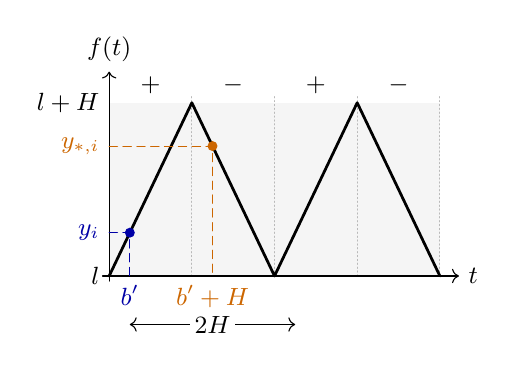
\begin{tikzpicture}[x=1.05cm,y=2.2cm,font=\small,
  line cap=round,line join=round]
  \path[fill=gray!8] (0,0) rectangle (4,1);
  \foreach \x in {0,1,2,3,4}
    \draw[gray!55,densely dotted] (\x,0) -- (\x,1.04);
  \draw[->] (-.08,0) -- (4.23,0) node[right] {$t$};
  \draw[->] (0,-.03) -- (0,1.18) node[above] {$f(t)$};
  \draw[line width=1pt] (0,0) -- (1,1) -- (2,0) -- (3,1) -- (4,0);
  \node[left] at (0,0) {$l$};
  \node[left] at (0,1) {$l+H$};
  \draw[blue!65!black,densely dashed] (0,.25) -- (.25,.25) -- (.25,0);
  \draw[orange!80!black,densely dashed] (0,.75) -- (1.25,.75) -- (1.25,0);
  \fill[blue!65!black] (.25,.25) circle (1.8pt);
  \fill[orange!80!black] (1.25,.75) circle (1.8pt);
  \node[left,text=blue!65!black] at (0,.25) {$y_i$};
  \node[left,text=orange!80!black] at (0,.75) {$y_{*,i}$};
  \node[below,text=blue!65!black] at (.25,0) {$b'$};
  \node[below,text=orange!80!black] at (1.25,0) {$b'+H$};
  \draw[<->] (.25,-.28) -- (2.25,-.28)
    node[midway,fill=white,inner sep=1.5pt] {$2H$};
  \foreach \x/\sign in {.5/+,1.5/-,2.5/+,3.5/-}
    \node at (\x,1.1) {$\sign$};
\end{tikzpicture}
\par\smallskip
{\small
$\displaystyle f(t+H)=2l+H-f(t),$\par
$\displaystyle y_i+y_{*,i}=2l+H.$\par\smallskip
The signs record the alternating\par orientations of successive cells.}
\end{minipage}\hfill
\begin{minipage}[t]{0.54\linewidth}
\centering
\textbf{(b) One successful column}\par\smallskip
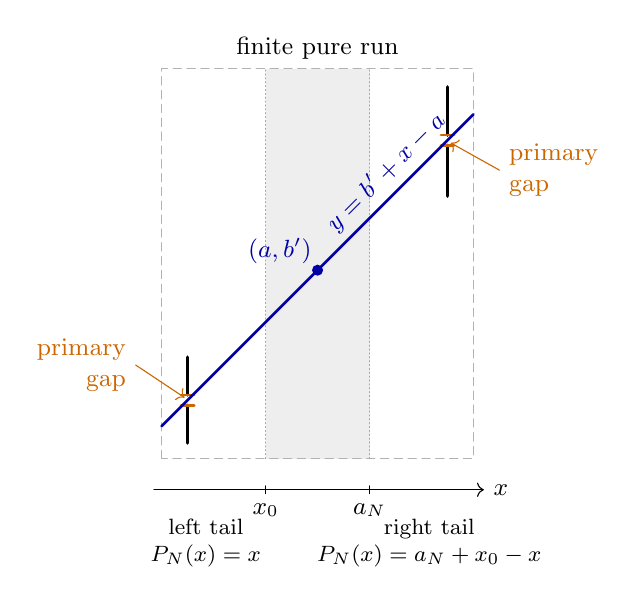
\begin{tikzpicture}[x=.33cm,y=.33cm,font=\small,
  line cap=round,line join=round]
  \path[fill=gray!13] (0,-7) rectangle (4,8);
  \draw[gray!60,densely dashed] (-4,-7) rectangle (8,8);
  \node[above,align=center] at (2,8) {finite pure run};
  \draw[gray!70,densely dotted] (0,-7) -- (0,8);
  \draw[gray!70,densely dotted] (4,-7) -- (4,8);
  \draw[line width=1.3pt] (-3,-6.4) -- (-3,-4.95);
  \draw[line width=1.3pt] (-3,-4.55) -- (-3,-3.1);
  \draw[line width=1.3pt] (7,3.1) -- (7,5.05);
  \draw[line width=1.3pt] (7,5.45) -- (7,7.3);
  \draw[orange!80!black,line width=1pt] (-3.25,-4.95) -- (-2.75,-4.95);
  \draw[orange!80!black,line width=1pt] (-3.25,-4.55) -- (-2.75,-4.55);
  \draw[orange!80!black,line width=1pt] (6.75,5.05) -- (7.25,5.05);
  \draw[orange!80!black,line width=1pt] (6.75,5.45) -- (7.25,5.45);
  \draw[blue!65!black,line width=1pt] (-4,-5.75) -- (8,6.25);
  \fill[blue!65!black] (2,.25) circle (2pt);
  \node[above left,text=blue!65!black,inner sep=2pt] at (2,.25) {$(a,b')$};
  \node[rotate=45,above,text=blue!65!black,inner sep=3pt]
    at (5.2,3.45) {$y=b'+x-a$};
  \draw[orange!80!black,->] (-5,-3.4) -- (-3.12,-4.65);
  \node[left,align=right,text=orange!80!black] at (-5,-3.4)
    {primary\\gap};
  \draw[orange!80!black,->] (9,4.1) -- (7.12,5.15);
  \node[right,align=left,text=orange!80!black] at (9,4.1)
    {primary\\gap};
  \draw[->] (-4.3,-8.2) -- (8.4,-8.2) node[right] {$x$};
  \draw (0,-8.05) -- (0,-8.35) node[below] {$x_0$};
  \draw (4,-8.05) -- (4,-8.35) node[below] {$a_N$};
  \node[align=center,font=\footnotesize] at (-2.3,-10.25)
    {left tail\\$P_N(x)=x$};
  \node[align=center,font=\footnotesize] at (6.3,-10.25)
    {right tail\\$P_N(x)=a_N+x_0-x$};
\end{tikzpicture}
\par\smallskip
{\small
$\displaystyle a\equiv X_*-H+O(\gamma)\pmod{2H}.$\par
Shading marks the central interval, whose image\par
$P_N([x_0,a_N])\subset[x_0-2H,x_0+v]$ is wall-free.}
\end{minipage}
\caption{The two coordinate projections in the final reflection construction.
Write $l=l_i$ and $H=H_i$.
Panel (a) shows the triangular projection to the original marker cell;
shifting a marker ordinate by an odd multiple of $H$ brings its projection
to the anchor height. In panel (b), only the tail-wall portions crossed by
one successful probe line are shown. At either tail wall $x_w$, the
congruence $x_w-a\equiv H+O(\gamma)\pmod{2H}$ places
$f(b'+x_w-a)$ inside a primary gap around $y_{*,i}$. The central
interval has no vertical-wall preimage. The pure run extends beyond the
line's passage through the finite horizontal support, so horizontal
solids are avoided as well. Gap-center crossings and distances are
schematic; the actual $O(\gamma)$ offsets fit within the primary openings.
Secondary gaps make the later fold cuts vacant and are not used for this
diagonal clearance.}
\label{fig:reflection-template-projections}
\end{figure}


Apply the vertical schedule for label $i$ only in word leaves
whose chosen majority label is $i$. All target copies lie on the
retained side of each such vertical fold. Their count doubles
there, while that child's weight is multiplied by $1/2$; their
expected count is therefore unchanged. Minority labels in the
other children are not discarded from the inequality: their total
expected count was already included in the unusable count of
Lemma~\ref{calc:word-purification}. Bad columns cost at most their
fraction times the expected count of the target label, which is
at most one. By choosing the run error and the column error each
less than $\varepsilon/4$, we obtain, for each original marker,
an expected favorable inventory of at least $1-\varepsilon/2$,
apart from coincidences of diagonal projections, addressed next.

\subsubsection{Vacant cuts, stability, and finite extraction}

The word and column constructions have produced the required favorable
inventory. It remains to realize their folds with vacant cuts, keep
the local source routes intact, and extract the favorable copies.
Only after these finite operations are fixed will we choose common
buffers and round to the lattice.

There are only finitely many cuts and copies in the tree just
constructed. Perturb their axis-cut coordinates by sufficiently
small fixed amounts. All successful primary-gap crossings and
pure-run buffers persist. We may require that no cut contain an
endpoint, marked feature, probe, or straight solid segment, and
that distinct insertion copies in any one leaf have distinct
diagonal-time projections $x-y$. To justify the last generic
choice, each copy coordinate is affine in the original coordinates
and in its ancestral cut coordinates. For two different reflection
histories, use the last cut at which the copy histories differ:
its coefficient in their coordinate difference is nonzero, and
subsequent common reflections preserve nonzero dependence.
Thus a coincidence of their diagonal projections is a proper
affine equation in the cuts. If their histories are the same but
their original markers differ, a possible coincidence reduces to
one of the two excluded axis-diagonal equalities for the original
probes. Avoiding finitely many proper affine equations is possible
in every open perturbation neighborhood. The same reasoning
avoids the finitely many incidences of cuts with tips and marked
features. After this perturbation all the retained favorable
copies have slabs avoiding the other insertion boxes as well.

At each transverse intersection of a cut with a solid, insert a
secondary gap at its preimage on the original wall. The generic
choice has kept every such preimage away from original marks,
corners, and primary-gap tips. There are only finitely many distinct
preimages. Merge repeated locations, and take their gap widths
small enough that their neighborhoods are pairwise disjoint and
avoid the protected features. In the reflected copies these gaps
make each prescribed axis cut vacant, with a positive margin. They
only remove solids, so cannot spoil any favorable slab. Source
strings crossing a cut do not constitute solids: their continuous
flux joins are the finite identities in
Proposition~\ref{prop:finite-extraction}. No probabilistic estimate
is being used to make a cut vacant.

We also track the local routing condition at the probes. An axis fold
restricts the diagram to one side and reflects it into the other;
because its cut has positive distance from every probe box, each
surviving box and its arriving prefix are copied intact. No foreign
chain enters a copied box. Any transverse flux join needed at the
cut is made within a vacant margin disjoint from all these boxes.
At a diagonal extraction, choose both the band and its spare routing
margins away from every other box, using their distinct diagonal
projections. Proposition~\ref{prop:finite-extraction} then alters only
the extracted box and these clear margins; all remaining boxes and
their prefixes are copied intact into the two norm diagrams. Induction
therefore preserves the chain-free neighborhood hypothesis for every
later extraction. In particular, this construction never reroutes a
diagonal chain across an unrelated source.

We now apply Lemma~\ref{lem:calc-median-extraction} to the
favorable inventory. The extraction bands contain no other marked
data, as required by Proposition~\ref{prop:finite-extraction}.
Since the preliminary tree has finitely many leaves, a common
finite depth makes their total expected residual favorable count
less than $\varepsilon/2$. Every extracted tagged marker is counted
once, and all other splits preserve tagged counts in half-average.
Combining this residual bound with the favorable inventory above
proves the extracted-count assertion.

Every tagged background feature, excluding all probe insertions,
is intact on one side of every cut and outside every removed middle band.
The two children therefore preserve its expected count. In either
individual child, each retained copy is paired with its mirror,
whose reflection parity is opposite. There was at least one
whole-word end fold, and every subsequent fold or norm split has
the same pairing property. Hence the terminal expected count of
each such feature is one, divided equally between its two
reflection parities. This also explains why the feature count
cannot be replaced by an estimate on arbitrary untracked state
norms.

All inequalities expressing separation in this finite successful
inventory are strict. Holding its chosen cuts and secondary-gap
locations fixed, they remain valid in a neighborhood of the
initial probe pair. A compact eligible set therefore admits a
finite cover by such neighborhoods and their templates. Take the
union of the finitely many secondary-gap locations, merging
coincident locations, and use a common sufficiently small positive
width. The additional vacancies only improve the clearances in
each template.  Shrink the covering neighborhoods to compact
subneighborhoods that still cover the eligible set.  For each
original tip, protected mark, or endpoint, take the minimum of its
strict clearances over every copy in these finite templates and
over every probe pair in the corresponding compact neighborhood.
These clearances include foreign solids and features, all probe
boxes, and every cut, extraction, and rerouting margin.  A smaller
buffered support at the original feature, transported unchanged to
all its copies, is therefore safe throughout the tree.  In
particular its radius does not depend on the actual probe pair.
Finally, round cut lines and gap ends to vertex
lines. Each error is $O(n^{-1})$, and only finitely many reflections
are involved. Thus the total displacement is $O(n^{-1})$ with a
template-dependent constant, smaller than every fixed clearance
for all sufficiently large $n$. The same observation covers all
bounded-mesh shifts of the original data and the local two-step
stencils. This proves Lemma~\ref{lem:reflection-templates}.
\end{proof}


\clearpage
\phantomsection
\addcontentsline{toc}{section}{References}
\bibliographystyle{plainnat}
\bibliography{references}
\end{document}
